\documentclass[twoside]{book}

% Packages required by doxygen
\usepackage{fixltx2e}
\usepackage{calc}
\usepackage{doxygen}
\usepackage[export]{adjustbox} % also loads graphicx
\usepackage{graphicx}
\usepackage[utf8]{inputenc}
\usepackage{makeidx}
\usepackage{multicol}
\usepackage{multirow}
\PassOptionsToPackage{warn}{textcomp}
\usepackage{textcomp}
\usepackage[nointegrals]{wasysym}
\usepackage[table]{xcolor}

% Font selection
\usepackage[T1]{fontenc}
\usepackage[scaled=.90]{helvet}
\usepackage{courier}
\usepackage{amssymb}
\usepackage{sectsty}
\renewcommand{\familydefault}{\sfdefault}
\allsectionsfont{%
  \fontseries{bc}\selectfont%
  \color{darkgray}%
}
\renewcommand{\DoxyLabelFont}{%
  \fontseries{bc}\selectfont%
  \color{darkgray}%
}
\newcommand{\+}{\discretionary{\mbox{\scriptsize$\hookleftarrow$}}{}{}}

% Page & text layout
\usepackage{geometry}
\geometry{%
  a4paper,%
  top=2.5cm,%
  bottom=2.5cm,%
  left=2.5cm,%
  right=2.5cm%
}
\tolerance=750
\hfuzz=15pt
\hbadness=750
\setlength{\emergencystretch}{15pt}
\setlength{\parindent}{0cm}
\setlength{\parskip}{3ex plus 2ex minus 2ex}
\makeatletter
\renewcommand{\paragraph}{%
  \@startsection{paragraph}{4}{0ex}{-1.0ex}{1.0ex}{%
    \normalfont\normalsize\bfseries\SS@parafont%
  }%
}
\renewcommand{\subparagraph}{%
  \@startsection{subparagraph}{5}{0ex}{-1.0ex}{1.0ex}{%
    \normalfont\normalsize\bfseries\SS@subparafont%
  }%
}
\makeatother

% Headers & footers
\usepackage{fancyhdr}
\pagestyle{fancyplain}
\fancyhead[LE]{\fancyplain{}{\bfseries\thepage}}
\fancyhead[CE]{\fancyplain{}{}}
\fancyhead[RE]{\fancyplain{}{\bfseries\leftmark}}
\fancyhead[LO]{\fancyplain{}{\bfseries\rightmark}}
\fancyhead[CO]{\fancyplain{}{}}
\fancyhead[RO]{\fancyplain{}{\bfseries\thepage}}
\fancyfoot[LE]{\fancyplain{}{}}
\fancyfoot[CE]{\fancyplain{}{}}
\fancyfoot[RE]{\fancyplain{}{\bfseries\scriptsize Generated by Doxygen }}
\fancyfoot[LO]{\fancyplain{}{\bfseries\scriptsize Generated by Doxygen }}
\fancyfoot[CO]{\fancyplain{}{}}
\fancyfoot[RO]{\fancyplain{}{}}
\renewcommand{\footrulewidth}{0.4pt}
\renewcommand{\chaptermark}[1]{%
  \markboth{#1}{}%
}
\renewcommand{\sectionmark}[1]{%
  \markright{\thesection\ #1}%
}

% Indices & bibliography
\usepackage{natbib}
\usepackage[titles]{tocloft}
\setcounter{tocdepth}{3}
\setcounter{secnumdepth}{5}
\makeindex

% Hyperlinks (required, but should be loaded last)
\usepackage{ifpdf}
\ifpdf
  \usepackage[pdftex,pagebackref=true]{hyperref}
\else
  \usepackage[ps2pdf,pagebackref=true]{hyperref}
\fi
\hypersetup{%
  colorlinks=true,%
  linkcolor=blue,%
  citecolor=blue,%
  unicode%
}

% Custom commands
\newcommand{\clearemptydoublepage}{%
  \newpage{\pagestyle{empty}\cleardoublepage}%
}

\usepackage{caption}
\captionsetup{labelsep=space,justification=centering,font={bf},singlelinecheck=off,skip=4pt,position=top}

%===== C O N T E N T S =====

\begin{document}

% Titlepage & ToC
\hypersetup{pageanchor=false,
             bookmarksnumbered=true,
             pdfencoding=unicode
            }
\pagenumbering{roman}
\begin{titlepage}
\vspace*{7cm}
\begin{center}%
{\Large exch2exch \\[1ex]\large 0.\+22 }\\
\vspace*{1cm}
{\large Generated by Doxygen 1.8.11}\\
\end{center}
\end{titlepage}
\clearemptydoublepage
\tableofcontents
\clearemptydoublepage
\pagenumbering{arabic}
\hypersetup{pageanchor=true}

%--- Begin generated contents ---
\chapter{R\+E\+A\+D\+ME}
\label{md__home_hilton_github_exch2exh_README}
\hypertarget{md__home_hilton_github_exch2exh_README}{}
A tool to compare Bitcoin rates in Brazil and overseas, to check if it would be nice buy there and sell locally. 
\chapter{Namespace Index}
\section{Packages}
Here are the packages with brief descriptions (if available)\-:\begin{DoxyCompactList}
\item\contentsline{section}{\hyperlink{namespaceexch2exch}{exch2exch} }{\pageref{namespaceexch2exch}}{}
\item\contentsline{section}{\hyperlink{namespaceexchange}{exchange} }{\pageref{namespaceexchange}}{}
\item\contentsline{section}{\hyperlink{namespaceraw__urlparser}{raw\-\_\-urlparser} }{\pageref{namespaceraw__urlparser}}{}
\end{DoxyCompactList}

\chapter{Hierarchical Index}
\section{Class Hierarchy}
This inheritance list is sorted roughly, but not completely, alphabetically\+:\begin{DoxyCompactList}
\item \contentsline{section}{e2e.\+Application}{\pageref{classe2e_1_1_application}}{}
\item \contentsline{section}{e2e.\+Args}{\pageref{classe2e_1_1_args}}{}
\item \contentsline{section}{raw\+\_\+urlparser.\+Differences}{\pageref{classraw__urlparser_1_1_differences}}{}
\item \contentsline{section}{exch2exch.\+Differences}{\pageref{classexch2exch_1_1_differences}}{}
\item \contentsline{section}{exchange.\+Differences}{\pageref{classexchange_1_1_differences}}{}
\begin{DoxyCompactList}
\item \contentsline{section}{exchange.\+Diff\+Orderbook}{\pageref{classexchange_1_1_diff_orderbook}}{}
\item \contentsline{section}{exchange.\+Diff\+Tracker}{\pageref{classexchange_1_1_diff_tracker}}{}
\item \contentsline{section}{exchange.\+Diff\+Trades}{\pageref{classexchange_1_1_diff_trades}}{}
\end{DoxyCompactList}
\item \contentsline{section}{gen\+\_\+factory.\+Dummy}{\pageref{classgen__factory_1_1_dummy}}{}
\begin{DoxyCompactList}
\item \contentsline{section}{gen\+\_\+factory.\+Dummy1}{\pageref{classgen__factory_1_1_dummy1}}{}
\item \contentsline{section}{gen\+\_\+factory.\+Dummy2}{\pageref{classgen__factory_1_1_dummy2}}{}
\item \contentsline{section}{gen\+\_\+factory.\+Dummy3}{\pageref{classgen__factory_1_1_dummy3}}{}
\end{DoxyCompactList}
\item \contentsline{section}{exchange.\+Exchange}{\pageref{classexchange_1_1_exchange}}{}
\begin{DoxyCompactList}
\item \contentsline{section}{exchange.\+Bitfinex}{\pageref{classexchange_1_1_bitfinex}}{}
\item \contentsline{section}{exchange.\+Bitstamp}{\pageref{classexchange_1_1_bitstamp}}{}
\item \contentsline{section}{exchange.\+Fox\+Bit}{\pageref{classexchange_1_1_fox_bit}}{}
\item \contentsline{section}{exchange.\+Mercado\+Bitcoin}{\pageref{classexchange_1_1_mercado_bitcoin}}{}
\item \contentsline{section}{exchange.\+Ok\+Coin}{\pageref{classexchange_1_1_ok_coin}}{}
\end{DoxyCompactList}
\item \contentsline{section}{gen\+\_\+factory.\+Gen\+Factory}{\pageref{classgen__factory_1_1_gen_factory}}{}
\item J\+S\+O\+N\+Encoder\begin{DoxyCompactList}
\item \contentsline{section}{exchange.\+Datetime\+Encoder}{\pageref{classexchange_1_1_datetime_encoder}}{}
\end{DoxyCompactList}
\item \contentsline{section}{exchange.\+Order\+Book}{\pageref{classexchange_1_1_order_book}}{}
\item \contentsline{section}{e2e.\+Parameters}{\pageref{classe2e_1_1_parameters}}{}
\item \contentsline{section}{rates.\+Rate}{\pageref{classrates_1_1_rate}}{}
\item \contentsline{section}{exch2exch.\+Rates}{\pageref{classexch2exch_1_1_rates}}{}
\item \contentsline{section}{raw\+\_\+urlparser.\+Rates}{\pageref{classraw__urlparser_1_1_rates}}{}
\item \contentsline{section}{rates.\+Rates}{\pageref{classrates_1_1_rates}}{}
\begin{DoxyCompactList}
\item \contentsline{section}{rates.\+Google}{\pageref{classrates_1_1_google}}{}
\item \contentsline{section}{rates.\+X\+Rates}{\pageref{classrates_1_1_x_rates}}{}
\end{DoxyCompactList}
\item \contentsline{section}{exchange.\+Ticker}{\pageref{classexchange_1_1_ticker}}{}
\item \contentsline{section}{exchange.\+Trades}{\pageref{classexchange_1_1_trades}}{}
\item \contentsline{section}{exch2exch.\+Xbt\+Prices}{\pageref{classexch2exch_1_1_xbt_prices}}{}
\item \contentsline{section}{raw\+\_\+urlparser.\+Xbt\+Prices}{\pageref{classraw__urlparser_1_1_xbt_prices}}{}
\end{DoxyCompactList}

\chapter{Class Index}
\section{Class List}
Here are the classes, structs, unions and interfaces with brief descriptions\+:\begin{DoxyCompactList}
\item\contentsline{section}{\hyperlink{classe2e_1_1_application}{e2e.\+Application} }{\pageref{classe2e_1_1_application}}{}
\item\contentsline{section}{\hyperlink{classe2e_1_1_args}{e2e.\+Args} }{\pageref{classe2e_1_1_args}}{}
\item\contentsline{section}{\hyperlink{classexchange_1_1_datetime_encoder}{exchange.\+Datetime\+Encoder} }{\pageref{classexchange_1_1_datetime_encoder}}{}
\item\contentsline{section}{\hyperlink{classexch2exch_1_1_differences}{exch2exch.\+Differences} }{\pageref{classexch2exch_1_1_differences}}{}
\item\contentsline{section}{\hyperlink{classraw__urlparser_1_1_differences}{raw\+\_\+urlparser.\+Differences} }{\pageref{classraw__urlparser_1_1_differences}}{}
\item\contentsline{section}{\hyperlink{classgen__factory_1_1_dummy}{gen\+\_\+factory.\+Dummy} }{\pageref{classgen__factory_1_1_dummy}}{}
\item\contentsline{section}{\hyperlink{classgen__factory_1_1_dummy1}{gen\+\_\+factory.\+Dummy1} }{\pageref{classgen__factory_1_1_dummy1}}{}
\item\contentsline{section}{\hyperlink{classgen__factory_1_1_dummy2}{gen\+\_\+factory.\+Dummy2} }{\pageref{classgen__factory_1_1_dummy2}}{}
\item\contentsline{section}{\hyperlink{classgen__factory_1_1_dummy3}{gen\+\_\+factory.\+Dummy3} }{\pageref{classgen__factory_1_1_dummy3}}{}
\item\contentsline{section}{\hyperlink{classexchange_1_1_exchange}{exchange.\+Exchange} }{\pageref{classexchange_1_1_exchange}}{}
\item\contentsline{section}{\hyperlink{classexchange_1_1_fox_bit}{exchange.\+Fox\+Bit} }{\pageref{classexchange_1_1_fox_bit}}{}
\item\contentsline{section}{\hyperlink{classgen__factory_1_1_gen_factory}{gen\+\_\+factory.\+Gen\+Factory} }{\pageref{classgen__factory_1_1_gen_factory}}{}
\item\contentsline{section}{\hyperlink{classrates_1_1_google}{rates.\+Google} }{\pageref{classrates_1_1_google}}{}
\item\contentsline{section}{\hyperlink{classexchange_1_1_mercado_bitcoin}{exchange.\+Mercado\+Bitcoin} }{\pageref{classexchange_1_1_mercado_bitcoin}}{}
\item\contentsline{section}{\hyperlink{classexchange_1_1_ok_coin}{exchange.\+Ok\+Coin} }{\pageref{classexchange_1_1_ok_coin}}{}
\item\contentsline{section}{\hyperlink{classexchange_1_1_order_book}{exchange.\+Order\+Book} }{\pageref{classexchange_1_1_order_book}}{}
\item\contentsline{section}{\hyperlink{classe2e_1_1_parameters}{e2e.\+Parameters} }{\pageref{classe2e_1_1_parameters}}{}
\item\contentsline{section}{\hyperlink{classrates_1_1_rate}{rates.\+Rate} }{\pageref{classrates_1_1_rate}}{}
\item\contentsline{section}{\hyperlink{classexch2exch_1_1_rates}{exch2exch.\+Rates} }{\pageref{classexch2exch_1_1_rates}}{}
\item\contentsline{section}{\hyperlink{classrates_1_1_rates}{rates.\+Rates} }{\pageref{classrates_1_1_rates}}{}
\item\contentsline{section}{\hyperlink{classraw__urlparser_1_1_rates}{raw\+\_\+urlparser.\+Rates} }{\pageref{classraw__urlparser_1_1_rates}}{}
\item\contentsline{section}{\hyperlink{classexchange_1_1_ticker}{exchange.\+Ticker} }{\pageref{classexchange_1_1_ticker}}{}
\item\contentsline{section}{\hyperlink{classexchange_1_1_trades}{exchange.\+Trades} }{\pageref{classexchange_1_1_trades}}{}
\item\contentsline{section}{\hyperlink{classraw__urlparser_1_1_xbt_prices}{raw\+\_\+urlparser.\+Xbt\+Prices} }{\pageref{classraw__urlparser_1_1_xbt_prices}}{}
\item\contentsline{section}{\hyperlink{classexch2exch_1_1_xbt_prices}{exch2exch.\+Xbt\+Prices} }{\pageref{classexch2exch_1_1_xbt_prices}}{}
\item\contentsline{section}{\hyperlink{classrates_1_1_x_rates}{rates.\+X\+Rates} }{\pageref{classrates_1_1_x_rates}}{}
\end{DoxyCompactList}

\chapter{File Index}
\section{File List}
Here is a list of all files with brief descriptions\+:\begin{DoxyCompactList}
\item\contentsline{section}{/home/hilton/github/exch2exh/\hyperlink{e2e_8py}{e2e.\+py} }{\pageref{e2e_8py}}{}
\item\contentsline{section}{/home/hilton/github/exch2exh/\hyperlink{exch2exch_8py}{exch2exch.\+py} }{\pageref{exch2exch_8py}}{}
\item\contentsline{section}{/home/hilton/github/exch2exh/\hyperlink{exchange_8py}{exchange.\+py} }{\pageref{exchange_8py}}{}
\item\contentsline{section}{/home/hilton/github/exch2exh/\hyperlink{exchange__server_8py}{exchange\+\_\+server.\+py} }{\pageref{exchange__server_8py}}{}
\item\contentsline{section}{/home/hilton/github/exch2exh/\hyperlink{gen__factory_8py}{gen\+\_\+factory.\+py} }{\pageref{gen__factory_8py}}{}
\item\contentsline{section}{/home/hilton/github/exch2exh/\hyperlink{rates_8py}{rates.\+py} }{\pageref{rates_8py}}{}
\item\contentsline{section}{/home/hilton/github/exch2exh/\hyperlink{raw__urlparser_8py}{raw\+\_\+urlparser.\+py} }{\pageref{raw__urlparser_8py}}{}
\end{DoxyCompactList}

\chapter{Namespace Documentation}
\hypertarget{namespacee2e}{}\section{e2e Namespace Reference}
\label{namespacee2e}\index{e2e@{e2e}}
\subsection*{Classes}
\begin{DoxyCompactItemize}
\item 
class \hyperlink{classe2e_1_1_application}{Application}
\item 
class \hyperlink{classe2e_1_1_args}{Args}
\item 
class \hyperlink{classe2e_1_1_parameters}{Parameters}
\end{DoxyCompactItemize}
\subsection*{Functions}
\begin{DoxyCompactItemize}
\item 
def \hyperlink{namespacee2e_afb3e7d384688a07b72e1df5201192375}{main} (argv)
\end{DoxyCompactItemize}


\subsection{Function Documentation}
\index{e2e@{e2e}!main@{main}}
\index{main@{main}!e2e@{e2e}}
\subsubsection[{\texorpdfstring{main(argv)}{main(argv)}}]{\setlength{\rightskip}{0pt plus 5cm}def e2e.\+main (
\begin{DoxyParamCaption}
\item[{}]{argv}
\end{DoxyParamCaption}
)}\hypertarget{namespacee2e_afb3e7d384688a07b72e1df5201192375}{}\label{namespacee2e_afb3e7d384688a07b72e1df5201192375}


Definition at line \hyperlink{e2e_8py_source_l00418}{418} of file \hyperlink{e2e_8py_source}{e2e.\+py}.


\begin{DoxyCode}
\hypertarget{namespacee2e.tex_l00418}{}\hyperlink{namespacee2e_afb3e7d384688a07b72e1df5201192375}{00418} \textcolor{keyword}{def }\hyperlink{namespacee2e_afb3e7d384688a07b72e1df5201192375}{main} (argv):
00419     app = Application ()
00420     
00421     \textcolor{comment}{# TODO parse command line }
00422     \textcolor{comment}{# TODO catch exception}
00423     \textcolor{comment}{# TODO return according to error}
00424     app.parseCmdLine ()
00425     
00426     \textcolor{comment}{# TODO interpret command line }
00427     \textcolor{comment}{# TODO catch exception}
00428     \textcolor{comment}{# TODO return according to error}
00429     app.interpretArgs ()
00430     
00431     \textcolor{comment}{# TODO consult main rate service}
00432     app.outMainRates ()
00433     
00434     \textcolor{comment}{# TODO consult all rate services}
00435     app.outAllRates ()
00436     
00437     \textcolor{comment}{# TODO consult origin exchange }
00438     app.outOriginExchange ()
00439     
00440     \textcolor{comment}{# TODO consult destination exchange}
00441     app.outDestinationExchange ()
00442     
00443     \textcolor{comment}{# TODO generate expectations}
00444     
00445     \textcolor{comment}{# TODO generate output report and JSON files}
00446 
00447     \textcolor{comment}{# Normal function termination}
00448     \textcolor{keywordflow}{return} 0
00449 
\end{DoxyCode}

\hypertarget{namespaceexch2exch}{\section{exch2exch Namespace Reference}
\label{namespaceexch2exch}\index{exch2exch@{exch2exch}}
}
\subsection*{Classes}
\begin{DoxyCompactItemize}
\item 
class \hyperlink{classexch2exch_1_1_differences}{Differences}
\item 
class \hyperlink{classexch2exch_1_1_rates}{Rates}
\item 
class \hyperlink{classexch2exch_1_1_xbt_prices}{Xbt\-Prices}
\end{DoxyCompactItemize}
\subsection*{Functions}
\begin{DoxyCompactItemize}
\item 
def \hyperlink{namespaceexch2exch_ab44bbb7377e2ea808af430246d925cd2}{get\-\_\-google\-\_\-rate}
\item 
def \hyperlink{namespaceexch2exch_a72e4d9fae01812560db07229c05efbc6}{get\-\_\-google\-\_\-rates}
\item 
def \hyperlink{namespaceexch2exch_a69c86b486350c524c85fca367aad82f2}{get\-\_\-mb\-\_\-rates}
\item 
def \hyperlink{namespaceexch2exch_a7e83d805e732ce4344cb3a6edc5d98be}{get\-\_\-ok\-\_\-rates}
\item 
def \hyperlink{namespaceexch2exch_a0fe4c93bea8fee4212c19f045c72b43b}{get\-\_\-x\-\_\-rates}
\item 
def \hyperlink{namespaceexch2exch_a559f55b08d308a647cc4afa3620e2da8}{main}
\end{DoxyCompactItemize}


\subsection{Function Documentation}
\hypertarget{namespaceexch2exch_ab44bbb7377e2ea808af430246d925cd2}{\index{exch2exch@{exch2exch}!get\-\_\-google\-\_\-rate@{get\-\_\-google\-\_\-rate}}
\index{get\-\_\-google\-\_\-rate@{get\-\_\-google\-\_\-rate}!exch2exch@{exch2exch}}
\subsubsection[{get\-\_\-google\-\_\-rate}]{\setlength{\rightskip}{0pt plus 5cm}def exch2exch.\-get\-\_\-google\-\_\-rate (
\begin{DoxyParamCaption}
\item[{}]{url}
\end{DoxyParamCaption}
)}}\label{namespaceexch2exch_ab44bbb7377e2ea808af430246d925cd2}


Definition at line 149 of file exch2exch.\-py.


\begin{DoxyCode}
149 
150 \textcolor{keyword}{def }\hyperlink{namespaceexch2exch_ab44bbb7377e2ea808af430246d925cd2}{get\_google\_rate} (url):
151     result = 0
152 
153     f = urllib.request.urlopen (url)
154     
155     line = f.readline ()
156     \textcolor{keywordflow}{while} line != b\textcolor{stringliteral}{''}:
157         ind = line.find (b\textcolor{stringliteral}{'currency\_converter'})
158         \textcolor{keywordflow}{if} ind != -1:
159             
160             fields = line.split ()
161             rate = fields[5].split (b\textcolor{stringliteral}{'>'})[1]
162             
163             \textcolor{keywordflow}{break}
164             
165         line = f.readline ()
166     
167     result = float (rate)
168     
169     \textcolor{keywordflow}{return} result
    
\end{DoxyCode}
\hypertarget{namespaceexch2exch_a72e4d9fae01812560db07229c05efbc6}{\index{exch2exch@{exch2exch}!get\-\_\-google\-\_\-rates@{get\-\_\-google\-\_\-rates}}
\index{get\-\_\-google\-\_\-rates@{get\-\_\-google\-\_\-rates}!exch2exch@{exch2exch}}
\subsubsection[{get\-\_\-google\-\_\-rates}]{\setlength{\rightskip}{0pt plus 5cm}def exch2exch.\-get\-\_\-google\-\_\-rates (
\begin{DoxyParamCaption}
\item[{}]{urls}
\end{DoxyParamCaption}
)}}\label{namespaceexch2exch_a72e4d9fae01812560db07229c05efbc6}


Definition at line 170 of file exch2exch.\-py.


\begin{DoxyCode}
170 
171 \textcolor{keyword}{def }\hyperlink{namespaceexch2exch_a72e4d9fae01812560db07229c05efbc6}{get\_google\_rates} (urls):
172     ts = math.trunc (time.time () + 0.5)
173     dt = datetime.datetime.fromtimestamp (ts)
174     
175     \textcolor{comment}{# TODO round the seconds fraction}
176     
177     usd2brl = urls[0]
178     brl2usd = urls[1]
179     
180     usd = 0
181     brl = 0
182     
183     usd = get\_google\_rate (usd2brl)
184     brl = get\_google\_rate (brl2usd)
185     
186     result = (dt, usd, brl)
187     
188     \textcolor{keywordflow}{return} result
        
\end{DoxyCode}
\hypertarget{namespaceexch2exch_a69c86b486350c524c85fca367aad82f2}{\index{exch2exch@{exch2exch}!get\-\_\-mb\-\_\-rates@{get\-\_\-mb\-\_\-rates}}
\index{get\-\_\-mb\-\_\-rates@{get\-\_\-mb\-\_\-rates}!exch2exch@{exch2exch}}
\subsubsection[{get\-\_\-mb\-\_\-rates}]{\setlength{\rightskip}{0pt plus 5cm}def exch2exch.\-get\-\_\-mb\-\_\-rates (
\begin{DoxyParamCaption}
\item[{}]{url}
\end{DoxyParamCaption}
)}}\label{namespaceexch2exch_a69c86b486350c524c85fca367aad82f2}


Definition at line 232 of file exch2exch.\-py.


\begin{DoxyCode}
232 
233 \textcolor{keyword}{def }\hyperlink{namespaceexch2exch_a69c86b486350c524c85fca367aad82f2}{get\_mb\_rates} (url):
234     f = urllib.request.urlopen (url)
235     
236     line = f.readline ()
237     
238     rv = json.loads (line.decode (encoding=\textcolor{stringliteral}{'utf-8'}))
239     
240     ts   = int   (rv[\textcolor{stringliteral}{'ticker'}][\textcolor{stringliteral}{'date'}])
241     buy  = float (rv[\textcolor{stringliteral}{'ticker'}][\textcolor{stringliteral}{'buy'}])
242     sell = float (rv[\textcolor{stringliteral}{'ticker'}][\textcolor{stringliteral}{'sell'}])
243     high = float (rv[\textcolor{stringliteral}{'ticker'}][\textcolor{stringliteral}{'high'}])
244     low  = float (rv[\textcolor{stringliteral}{'ticker'}][\textcolor{stringliteral}{'low'}])
245     
246     dt = datetime.datetime.fromtimestamp (float (ts))
247     
248     result = (dt, sell, buy, high, low)
249     
250     \textcolor{keywordflow}{return} result

\end{DoxyCode}
\hypertarget{namespaceexch2exch_a7e83d805e732ce4344cb3a6edc5d98be}{\index{exch2exch@{exch2exch}!get\-\_\-ok\-\_\-rates@{get\-\_\-ok\-\_\-rates}}
\index{get\-\_\-ok\-\_\-rates@{get\-\_\-ok\-\_\-rates}!exch2exch@{exch2exch}}
\subsubsection[{get\-\_\-ok\-\_\-rates}]{\setlength{\rightskip}{0pt plus 5cm}def exch2exch.\-get\-\_\-ok\-\_\-rates (
\begin{DoxyParamCaption}
\item[{}]{url}
\end{DoxyParamCaption}
)}}\label{namespaceexch2exch_a7e83d805e732ce4344cb3a6edc5d98be}


Definition at line 251 of file exch2exch.\-py.


\begin{DoxyCode}
251 
252 \textcolor{keyword}{def }\hyperlink{namespaceexch2exch_a7e83d805e732ce4344cb3a6edc5d98be}{get\_ok\_rates} (url):
253     f = urllib.request.urlopen (url)
254     
255     line = f.readline ()
256     
257     rv = json.loads (line.decode (encoding=\textcolor{stringliteral}{'utf-8'}))
258     
259     ts   = int   (rv[\textcolor{stringliteral}{'date'}])
260     buy  = float (rv[\textcolor{stringliteral}{'ticker'}][\textcolor{stringliteral}{'buy'}])
261     sell = float (rv[\textcolor{stringliteral}{'ticker'}][\textcolor{stringliteral}{'sell'}])
262     high = float (rv[\textcolor{stringliteral}{'ticker'}][\textcolor{stringliteral}{'high'}])
263     low  = float (rv[\textcolor{stringliteral}{'ticker'}][\textcolor{stringliteral}{'low'}])
264     
265     dt = datetime.datetime.fromtimestamp (float (ts))
266     
267     result = (dt, sell, buy, high, low)
268     
269     \textcolor{keywordflow}{return} result

\end{DoxyCode}
\hypertarget{namespaceexch2exch_a0fe4c93bea8fee4212c19f045c72b43b}{\index{exch2exch@{exch2exch}!get\-\_\-x\-\_\-rates@{get\-\_\-x\-\_\-rates}}
\index{get\-\_\-x\-\_\-rates@{get\-\_\-x\-\_\-rates}!exch2exch@{exch2exch}}
\subsubsection[{get\-\_\-x\-\_\-rates}]{\setlength{\rightskip}{0pt plus 5cm}def exch2exch.\-get\-\_\-x\-\_\-rates (
\begin{DoxyParamCaption}
\item[{}]{url}
\end{DoxyParamCaption}
)}}\label{namespaceexch2exch_a0fe4c93bea8fee4212c19f045c72b43b}


Definition at line 189 of file exch2exch.\-py.


\begin{DoxyCode}
189 
190 \textcolor{keyword}{def }\hyperlink{namespaceexch2exch_a0fe4c93bea8fee4212c19f045c72b43b}{get\_x\_rates} (url):
191     ts = math.trunc (time.time () + 0.5)
192     dt = datetime.datetime.fromtimestamp (ts)
193     
194     \textcolor{comment}{# TODO round the seconds fraction}
195     
196     \textcolor{comment}{# Adding a fake browser User-Agent to make site x-rates.com happy}
197     headers = \{\textcolor{stringliteral}{'User-Agent'} : \textcolor{stringliteral}{'Mozilla 5.10'}\}
198         
199     \textcolor{comment}{# Create the Request, joining URL and User-Agent}
200     request = urllib.request.Request (url, headers = headers)
201 
202     \textcolor{comment}{# Open the URL as file}
203     f = urllib.request.urlopen (request)
204     
205     \textcolor{comment}{# Input over the file to get the rates}
206     line = \textcolor{keywordtype}{None}
207     \textcolor{keywordflow}{while} line != b\textcolor{stringliteral}{''}:
208         line = f.readline ()
209         ind = line.find (b\textcolor{stringliteral}{'BRL'})
210         \textcolor{keywordflow}{if} ind == -1:
211             \textcolor{keywordflow}{continue} 
212         
213         ind = line.find (b\textcolor{stringliteral}{'rtRates'})
214         \textcolor{keywordflow}{if} ind == -1:
215             \textcolor{keywordflow}{continue} 
216                 
217         \textcolor{keywordflow}{if} line.find (b\textcolor{stringliteral}{'from=USD'}) != -1:
218             fields = line.split (b\textcolor{stringliteral}{'>'})
219             
220             susd = fields[2].split (b\textcolor{stringliteral}{'<'})[0]
221             usd = float (susd)
222         
223         \textcolor{keywordflow}{elif} line.find (b\textcolor{stringliteral}{'from=BRL'}) != -1:
224             fields = line.split (b\textcolor{stringliteral}{'>'})
225             
226             sbrl = fields[2].split (b\textcolor{stringliteral}{'<'})[0]
227             brl = float (sbrl)
228             
229     result = (dt, usd, brl)
230     
231     \textcolor{keywordflow}{return} result

\end{DoxyCode}
\hypertarget{namespaceexch2exch_a559f55b08d308a647cc4afa3620e2da8}{\index{exch2exch@{exch2exch}!main@{main}}
\index{main@{main}!exch2exch@{exch2exch}}
\subsubsection[{main}]{\setlength{\rightskip}{0pt plus 5cm}def exch2exch.\-main (
\begin{DoxyParamCaption}
{}
\end{DoxyParamCaption}
)}}\label{namespaceexch2exch_a559f55b08d308a647cc4afa3620e2da8}


Definition at line 270 of file exch2exch.\-py.


\begin{DoxyCode}
270 
271 \textcolor{keyword}{def }\hyperlink{namespaceexch2exch_a559f55b08d308a647cc4afa3620e2da8}{main} ():
272     \textcolor{comment}{# TODO parse command line }
273 
274     u\_usd2brl = \textcolor{stringliteral}{'https://www.google.com/finance/converter?a=1&from=USD&to=BRL'}
275     u\_brl2usd = \textcolor{stringliteral}{'https://www.google.com/finance/converter?a=1&from=BRL&to=USD'}
276 \textcolor{comment}{#    u\_mb      = 'https://www.mercadobitcoin.net/api/ticker/'}
277     u\_xrates  = \textcolor{stringliteral}{'http://www.x-rates.com/table/?from=USD&amount=1'}
278 \textcolor{comment}{#    u\_ok      = 'https://www.okcoin.com/api/v1/ticker.do?symbol=btc\_usd'}
279     
280     urls = (u\_usd2brl, u\_brl2usd)
281     
282     dt, usd2brl, brl2usd = get\_google\_rates (urls)
283     
284     google = Rates (dt, usd2brl, brl2usd, \textcolor{stringliteral}{"Google"})
285     
286     \textcolor{keywordflow}{print} (\textcolor{stringliteral}{"\{0\}\(\backslash\)n"}.format (google))
287     
288     \textcolor{comment}{#}
289     \textcolor{comment}{#}
290     \textcolor{comment}{# X-rates section }
291     \textcolor{comment}{# }
292     
293     dt, brl2usd, usd2brl = get\_x\_rates (u\_xrates)
294     
295     x\_rates = Rates (dt, brl2usd, usd2brl, \textcolor{stringliteral}{"X-Rates"})
296     
297     \textcolor{keywordflow}{print} (\textcolor{stringliteral}{"\{0\}\(\backslash\)n"}.format (x\_rates))
298     
299     \textcolor{comment}{# TODO calculate avg USD2BRL rate}
300     
301     \textcolor{comment}{#}
302     \textcolor{comment}{#}
303     \textcolor{comment}{# MercadoBitcoin section }
304     \textcolor{comment}{# }
305     
306     mb = \hyperlink{classexchange_1_1_mercado_bitcoin}{exchange.MercadoBitcoin} ()    
307 \textcolor{comment}{#    mb\_tupl = get\_mb\_rates (u\_mb)}
308     mb\_tupl = mb.get\_ticker ()
309     
310     dt, sell, buy, high, low = mb\_tupl
311     
312     mb = XbtPrices (dt, sell, buy, high, low, \textcolor{stringliteral}{"MercadoBitcoin"}, \textcolor{stringliteral}{"BRL"})
313     
314     \textcolor{comment}{# print ("MercadoBitcoin: \{0\}: Sell \{1\} BRL, Buy \{2\} BRL".format (mb))}
315     \textcolor{keywordflow}{print} (mb)
316      
317     brl2usd = google.getUsd2Brl ()
318     
319     sell /= brl2usd
320     buy  /= brl2usd 
321     high /= brl2usd
322     low  /= brl2usd 
323     mb\_usd = XbtPrices (dt, sell, buy, high, low, \textcolor{stringliteral}{"MercadoBitcoin"}, \textcolor{stringliteral}{"USD"})
324     \textcolor{keywordflow}{print} (\textcolor{stringliteral}{"\{0\}\(\backslash\)n"}.format (mb\_usd))
325     
326     \textcolor{comment}{#}
327     \textcolor{comment}{#}
328     \textcolor{comment}{# OkCoin section }
329     \textcolor{comment}{# }
330     
331 
332     ok = \hyperlink{classexchange_1_1_ok_coin}{exchange.OkCoin} ()        
333 \textcolor{comment}{#    ok\_tupl = get\_ok\_rates (u\_ok)}
334     ok\_tupl = ok.get\_ticker ()
335     
336     dt, sell, buy, high, low = ok\_tupl
337     
338     ok = XbtPrices (dt, sell, buy, high, low, \textcolor{stringliteral}{"OkCoin"}, \textcolor{stringliteral}{"USD"})
339     
340     \textcolor{comment}{# print ("MercadoBitcoin: \{0\}: Sell \{1\} BRL, Buy \{2\} BRL".format (mb))}
341     \textcolor{keywordflow}{print} (\textcolor{stringliteral}{"\{0\}\(\backslash\)n"}.format (ok))
342      
343     
344     diff = Differences (google, mb\_usd, ok)
345     
346     \textcolor{keywordflow}{print} (diff)
347     
348     \textcolor{keywordflow}{return} 0
    
\end{DoxyCode}

\hypertarget{namespaceexchange}{\section{exchange Namespace Reference}
\label{namespaceexchange}\index{exchange@{exchange}}
}
\subsection*{Classes}
\begin{DoxyCompactItemize}
\item 
class \hyperlink{classexchange_1_1_exchange}{Exchange}
\item 
class \hyperlink{classexchange_1_1_fox_bit}{Fox\-Bit}
\item 
class \hyperlink{classexchange_1_1_mercado_bitcoin}{Mercado\-Bitcoin}
\item 
class \hyperlink{classexchange_1_1_ok_coin}{Ok\-Coin}
\end{DoxyCompactItemize}
\subsection*{Functions}
\begin{DoxyCompactItemize}
\item 
def \hyperlink{namespaceexchange_adf14f1c5a512c2d8a7ece6e64e546916}{main}
\end{DoxyCompactItemize}


\subsection{Function Documentation}
\hypertarget{namespaceexchange_adf14f1c5a512c2d8a7ece6e64e546916}{\index{exchange@{exchange}!main@{main}}
\index{main@{main}!exchange@{exchange}}
\subsubsection[{main}]{\setlength{\rightskip}{0pt plus 5cm}def exchange.\-main (
\begin{DoxyParamCaption}
{}
\end{DoxyParamCaption}
)}}\label{namespaceexchange_adf14f1c5a512c2d8a7ece6e64e546916}


Definition at line 205 of file exchange.\-py.


\begin{DoxyCode}
205 
206 \textcolor{keyword}{def }\hyperlink{namespaceexchange_adf14f1c5a512c2d8a7ece6e64e546916}{main} ():
207     exchanges = []
208     exchanges.append (FoxBit ())
209     exchanges.append (MercadoBitcoin ())
210     exchanges.append (OkCoin ())
211     
212     \textcolor{keywordflow}{for} exch \textcolor{keywordflow}{in} exchanges:
213         exch.get\_ticker ()
214         
215         \textcolor{keywordflow}{print} (\textcolor{stringliteral}{"\{0\}: \{1\}"}.format (exch.get\_exch\_name (), exch))
216     
217     \textcolor{keywordflow}{return} 0
    
\end{DoxyCode}

\hypertarget{namespaceexchange__server}{}\section{exchange\+\_\+server Namespace Reference}
\label{namespaceexchange__server}\index{exchange\+\_\+server@{exchange\+\_\+server}}

\hypertarget{namespacegen__factory}{}\section{gen\+\_\+factory Namespace Reference}
\label{namespacegen__factory}\index{gen\+\_\+factory@{gen\+\_\+factory}}
\subsection*{Classes}
\begin{DoxyCompactItemize}
\item 
class \hyperlink{classgen__factory_1_1_dummy}{Dummy}
\item 
class \hyperlink{classgen__factory_1_1_dummy1}{Dummy1}
\item 
class \hyperlink{classgen__factory_1_1_dummy2}{Dummy2}
\item 
class \hyperlink{classgen__factory_1_1_dummy3}{Dummy3}
\item 
class \hyperlink{classgen__factory_1_1_gen_factory}{Gen\+Factory}
\end{DoxyCompactItemize}
\subsection*{Functions}
\begin{DoxyCompactItemize}
\item 
def \hyperlink{namespacegen__factory_a785bd40533dd477ffff224d65ba1c5c3}{main} ()
\end{DoxyCompactItemize}


\subsection{Function Documentation}
\mbox{\Hypertarget{namespacegen__factory_a785bd40533dd477ffff224d65ba1c5c3}\label{namespacegen__factory_a785bd40533dd477ffff224d65ba1c5c3}} 
\index{gen\+\_\+factory@{gen\+\_\+factory}!main@{main}}
\index{main@{main}!gen\+\_\+factory@{gen\+\_\+factory}}
\subsubsection{\texorpdfstring{main()}{main()}}
{\footnotesize\ttfamily def gen\+\_\+factory.\+main (\begin{DoxyParamCaption}{ }\end{DoxyParamCaption})}



Definition at line \hyperlink{gen__factory_8py_source_l00084}{84} of file \hyperlink{gen__factory_8py_source}{gen\+\_\+factory.\+py}.


\begin{DoxyCode}
00084 \textcolor{keyword}{def }\hyperlink{namespacegen__factory_a785bd40533dd477ffff224d65ba1c5c3}{main} ():
00085     gf = GenFactory (Dummy)
00086     
00087 \textcolor{comment}{#    obj = gf.genObject ("Dummy2")}
00088 \textcolor{comment}{#    }
00089 \textcolor{comment}{#    nam = type (obj).\_\_name\_\_ }
00090 \textcolor{comment}{#    print ("type (obj).\_\_name\_\_ = \{0\}".format (nam))}
00091 \textcolor{comment}{#    }
00092 \textcolor{comment}{#    obj.doSomething ()}
00093 \textcolor{comment}{#    print ("="*12)}
00094     
00095     \textcolor{keywordflow}{for} cn \textcolor{keywordflow}{in} gf.validClassNames ():
00096         \textcolor{keywordflow}{print} (\textcolor{stringliteral}{"Class \{0\}"}.format (cn))
00097         obj = gf.genObject (cn)
00098     
00099         nam = type (obj).\_\_name\_\_ 
00100         \textcolor{keywordflow}{print} (\textcolor{stringliteral}{"type (obj).\_\_name\_\_ = \{0\}"}.format (nam))
00101         obj.doSomething ()
00102         \textcolor{keywordflow}{print} ()
00103         
00104     \textcolor{comment}{# Normal function termination}
00105     \textcolor{keywordflow}{return} 0
00106 
\end{DoxyCode}

\hypertarget{namespacerates}{}\section{rates Namespace Reference}
\label{namespacerates}\index{rates@{rates}}
\subsection*{Classes}
\begin{DoxyCompactItemize}
\item 
class \hyperlink{classrates_1_1_google}{Google}
\item 
class \hyperlink{classrates_1_1_rate}{Rate}
\item 
class \hyperlink{classrates_1_1_rates}{Rates}
\item 
class \hyperlink{classrates_1_1_x_rates}{X\+Rates}
\end{DoxyCompactItemize}
\subsection*{Functions}
\begin{DoxyCompactItemize}
\item 
def \hyperlink{namespacerates_a2f1a70c33ee9e255938e4c19fd207264}{\+\_\+\+\_\+str\+\_\+\+\_\+} (self)
\item 
def \hyperlink{namespacerates_a083f2cdcd71554d301bcbfb0779ffa49}{get\+Brl2\+Usd} (self)
\item 
def \hyperlink{namespacerates_a5dd7b6601bc66e313c26984e32f1e290}{get\+Service\+Name} (self)
\item 
def \hyperlink{namespacerates_aafc179b32863137b88c74dd0ee2576bd}{get\+Service\+Prefix} (self)
\item 
def \hyperlink{namespacerates_ae4c7203ef8a919f9cf522581ca00b08a}{get\+Usd2\+Brl} (self)
\end{DoxyCompactItemize}


\subsection{Function Documentation}
\index{rates@{rates}!\+\_\+\+\_\+str\+\_\+\+\_\+@{\+\_\+\+\_\+str\+\_\+\+\_\+}}
\index{\+\_\+\+\_\+str\+\_\+\+\_\+@{\+\_\+\+\_\+str\+\_\+\+\_\+}!rates@{rates}}
\subsubsection[{\texorpdfstring{\+\_\+\+\_\+str\+\_\+\+\_\+(self)}{__str__(self)}}]{\setlength{\rightskip}{0pt plus 5cm}def rates.\+\_\+\+\_\+str\+\_\+\+\_\+ (
\begin{DoxyParamCaption}
\item[{}]{self}
\end{DoxyParamCaption}
)}\hypertarget{namespacerates_a2f1a70c33ee9e255938e4c19fd207264}{}\label{namespacerates_a2f1a70c33ee9e255938e4c19fd207264}


Definition at line \hyperlink{rates_8py_source_l00036}{36} of file \hyperlink{rates_8py_source}{rates.\+py}.


\begin{DoxyCode}
\hypertarget{namespacerates.tex_l00036}{}\hyperlink{namespacerates_a2f1a70c33ee9e255938e4c19fd207264}{00036}     \textcolor{keyword}{def }\hyperlink{namespacerates_a2f1a70c33ee9e255938e4c19fd207264}{\_\_str\_\_} (self):
00037         result = \textcolor{stringliteral}{''}
00038 
00039         service = self.service
00040         dt      = self.dt
00041         usd2brl = self.usd2brl
00042         brl2usd = self.brl2usd
00043         ftupl = (service, dt, usd2brl, brl2usd)
00044         
00045         result = \textcolor{stringliteral}{"\{0\}: \{1\}: USD2BRL \{2:.4f\}, BRL2USD \{3:.4f\}"}.format (*ftupl)
00046 
00047         \textcolor{keywordflow}{return} result        
00048     
\end{DoxyCode}
\index{rates@{rates}!get\+Brl2\+Usd@{get\+Brl2\+Usd}}
\index{get\+Brl2\+Usd@{get\+Brl2\+Usd}!rates@{rates}}
\subsubsection[{\texorpdfstring{get\+Brl2\+Usd(self)}{getBrl2Usd(self)}}]{\setlength{\rightskip}{0pt plus 5cm}def rates.\+get\+Brl2\+Usd (
\begin{DoxyParamCaption}
\item[{}]{self}
\end{DoxyParamCaption}
)}\hypertarget{namespacerates_a083f2cdcd71554d301bcbfb0779ffa49}{}\label{namespacerates_a083f2cdcd71554d301bcbfb0779ffa49}


Definition at line \hyperlink{rates_8py_source_l00024}{24} of file \hyperlink{rates_8py_source}{rates.\+py}.


\begin{DoxyCode}
\hypertarget{namespacerates.tex_l00024}{}\hyperlink{namespacerates_a083f2cdcd71554d301bcbfb0779ffa49}{00024}     \textcolor{keyword}{def }\hyperlink{namespacerates_a083f2cdcd71554d301bcbfb0779ffa49}{getBrl2Usd} (self):
00025         \textcolor{keywordflow}{return} self.brl2usd
00026     
\end{DoxyCode}
\index{rates@{rates}!get\+Service\+Name@{get\+Service\+Name}}
\index{get\+Service\+Name@{get\+Service\+Name}!rates@{rates}}
\subsubsection[{\texorpdfstring{get\+Service\+Name(self)}{getServiceName(self)}}]{\setlength{\rightskip}{0pt plus 5cm}def rates.\+get\+Service\+Name (
\begin{DoxyParamCaption}
\item[{}]{self}
\end{DoxyParamCaption}
)}\hypertarget{namespacerates_a5dd7b6601bc66e313c26984e32f1e290}{}\label{namespacerates_a5dd7b6601bc66e313c26984e32f1e290}


Definition at line \hyperlink{rates_8py_source_l00030}{30} of file \hyperlink{rates_8py_source}{rates.\+py}.


\begin{DoxyCode}
\hypertarget{namespacerates.tex_l00030}{}\hyperlink{namespacerates_a5dd7b6601bc66e313c26984e32f1e290}{00030}     \textcolor{keyword}{def }\hyperlink{namespacerates_a5dd7b6601bc66e313c26984e32f1e290}{getServiceName} (self):
00031         \textcolor{keywordflow}{return} self.service
00032     
\end{DoxyCode}
\index{rates@{rates}!get\+Service\+Prefix@{get\+Service\+Prefix}}
\index{get\+Service\+Prefix@{get\+Service\+Prefix}!rates@{rates}}
\subsubsection[{\texorpdfstring{get\+Service\+Prefix(self)}{getServicePrefix(self)}}]{\setlength{\rightskip}{0pt plus 5cm}def rates.\+get\+Service\+Prefix (
\begin{DoxyParamCaption}
\item[{}]{self}
\end{DoxyParamCaption}
)}\hypertarget{namespacerates_aafc179b32863137b88c74dd0ee2576bd}{}\label{namespacerates_aafc179b32863137b88c74dd0ee2576bd}


Definition at line \hyperlink{rates_8py_source_l00033}{33} of file \hyperlink{rates_8py_source}{rates.\+py}.


\begin{DoxyCode}
\hypertarget{namespacerates.tex_l00033}{}\hyperlink{namespacerates_aafc179b32863137b88c74dd0ee2576bd}{00033}     \textcolor{keyword}{def }\hyperlink{namespacerates_aafc179b32863137b88c74dd0ee2576bd}{getServicePrefix} (self):
00034         \textcolor{keywordflow}{return} self.prefix
00035         
\end{DoxyCode}
\index{rates@{rates}!get\+Usd2\+Brl@{get\+Usd2\+Brl}}
\index{get\+Usd2\+Brl@{get\+Usd2\+Brl}!rates@{rates}}
\subsubsection[{\texorpdfstring{get\+Usd2\+Brl(self)}{getUsd2Brl(self)}}]{\setlength{\rightskip}{0pt plus 5cm}def rates.\+get\+Usd2\+Brl (
\begin{DoxyParamCaption}
\item[{}]{self}
\end{DoxyParamCaption}
)}\hypertarget{namespacerates_ae4c7203ef8a919f9cf522581ca00b08a}{}\label{namespacerates_ae4c7203ef8a919f9cf522581ca00b08a}


Definition at line \hyperlink{rates_8py_source_l00027}{27} of file \hyperlink{rates_8py_source}{rates.\+py}.


\begin{DoxyCode}
\hypertarget{namespacerates.tex_l00027}{}\hyperlink{namespacerates_ae4c7203ef8a919f9cf522581ca00b08a}{00027}     \textcolor{keyword}{def }\hyperlink{namespacerates_ae4c7203ef8a919f9cf522581ca00b08a}{getUsd2Brl} (self):
00028         \textcolor{keywordflow}{return} self.usd2brl
00029     
\end{DoxyCode}

\hypertarget{namespaceraw__urlparser}{\section{raw\-\_\-urlparser Namespace Reference}
\label{namespaceraw__urlparser}\index{raw\-\_\-urlparser@{raw\-\_\-urlparser}}
}
\subsection*{Classes}
\begin{DoxyCompactItemize}
\item 
class \hyperlink{classraw__urlparser_1_1_differences}{Differences}
\item 
class \hyperlink{classraw__urlparser_1_1_rates}{Rates}
\item 
class \hyperlink{classraw__urlparser_1_1_xbt_prices}{Xbt\-Prices}
\end{DoxyCompactItemize}
\subsection*{Functions}
\begin{DoxyCompactItemize}
\item 
def \hyperlink{namespaceraw__urlparser_a27ce239a7915c6468e00168213575365}{get\-\_\-google\-\_\-rate}
\item 
def \hyperlink{namespaceraw__urlparser_a503f638b00ab579b8b829e1dbb95e547}{get\-\_\-google\-\_\-rates}
\item 
def \hyperlink{namespaceraw__urlparser_a56532368ca9848b5f2ab298e3e6232bb}{get\-\_\-mb\-\_\-rates}
\item 
def \hyperlink{namespaceraw__urlparser_a3a9d9300bd89d803ca1fddb78145f58e}{get\-\_\-ok\-\_\-rates}
\item 
def \hyperlink{namespaceraw__urlparser_a264ca664879b007ee92399e30ec0d9bc}{get\-\_\-x\-\_\-rates}
\end{DoxyCompactItemize}
\subsection*{Variables}
\begin{DoxyCompactItemize}
\item 
tuple \hyperlink{namespaceraw__urlparser_a382c2b22f2386b1e493674c7d72b9b95}{brl2usd} = google.\-get\-Usd2\-Brl()
\item 
tuple \hyperlink{namespaceraw__urlparser_a2a48999f60075fd5b96e6d540cce34c9}{diff} = \hyperlink{classraw__urlparser_1_1_differences}{Differences}(\hyperlink{namespaceraw__urlparser_a8d7c05a0ed7b2f3a3014caa73a2999d1}{google}, \hyperlink{namespaceraw__urlparser_a49f2920b4f7718df58d6d996a1306f32}{mb\-\_\-usd}, \hyperlink{namespaceraw__urlparser_ac9d30be4f20423526dc111ebaba51cfe}{ok})
\item 
tuple \hyperlink{namespaceraw__urlparser_a8d7c05a0ed7b2f3a3014caa73a2999d1}{google} = \hyperlink{classraw__urlparser_1_1_rates}{Rates}(dt, usd2brl, \hyperlink{namespaceraw__urlparser_a382c2b22f2386b1e493674c7d72b9b95}{brl2usd}, \char`\"{}Google\char`\"{})
\item 
tuple \hyperlink{namespaceraw__urlparser_a964275295a1dcba5dbdc3b113a75c4bb}{mb} = \hyperlink{classraw__urlparser_1_1_xbt_prices}{Xbt\-Prices}(dt, sell, buy, \char`\"{}Mercado\-Bitcoin\char`\"{}, \char`\"{}B\-R\-L\char`\"{})
\item 
tuple \hyperlink{namespaceraw__urlparser_ac8242502920772d4c44b42f24492acd5}{mb\-\_\-tupl} = \hyperlink{namespaceraw__urlparser_a56532368ca9848b5f2ab298e3e6232bb}{get\-\_\-mb\-\_\-rates}(\hyperlink{namespaceraw__urlparser_a9a840f174b92a24c415b88c87e84b73d}{u\-\_\-mb})
\item 
tuple \hyperlink{namespaceraw__urlparser_a49f2920b4f7718df58d6d996a1306f32}{mb\-\_\-usd} = \hyperlink{classraw__urlparser_1_1_xbt_prices}{Xbt\-Prices}(dt, sell, buy, \char`\"{}Mercado\-Bitcoin\char`\"{}, \char`\"{}U\-S\-D\char`\"{})
\item 
tuple \hyperlink{namespaceraw__urlparser_ac9d30be4f20423526dc111ebaba51cfe}{ok} = \hyperlink{classraw__urlparser_1_1_xbt_prices}{Xbt\-Prices}(dt, sell, buy, \char`\"{}Ok\-Coin\char`\"{}, \char`\"{}U\-S\-D\char`\"{})
\item 
tuple \hyperlink{namespaceraw__urlparser_a8c2d43346322c5d31fa8cb1a9cf5c121}{ok\-\_\-tupl} = \hyperlink{namespaceraw__urlparser_a3a9d9300bd89d803ca1fddb78145f58e}{get\-\_\-ok\-\_\-rates}(\hyperlink{namespaceraw__urlparser_a22c1a17803a88426d38d70ad6d4290d2}{u\-\_\-ok})
\item 
string \hyperlink{namespaceraw__urlparser_a876711ddd7ebb3991a35cc1768d1d22c}{u\-\_\-brl2usd} = 'https\-://www.\-google.\-com/finance/converter?a=1\&from=B\-R\-L\&to=U\-S\-D'
\item 
string \hyperlink{namespaceraw__urlparser_a9a840f174b92a24c415b88c87e84b73d}{u\-\_\-mb} = 'https\-://www.\-mercadobitcoin.\-net/api/ticker/'
\item 
string \hyperlink{namespaceraw__urlparser_a22c1a17803a88426d38d70ad6d4290d2}{u\-\_\-ok} = 'https\-://www.\-okcoin.\-com/api/v1/ticker.\-do?symbol=btc\-\_\-usd'
\item 
string \hyperlink{namespaceraw__urlparser_a63e1f0abe7b1f43c4891ce9aec98261d}{u\-\_\-usd2brl} = 'https\-://www.\-google.\-com/finance/converter?a=1\&from=U\-S\-D\&to=B\-R\-L'
\item 
string \hyperlink{namespaceraw__urlparser_a9242b893f4f49ef7cc0d4e599b70daa4}{url} = 'http\-://www.\-x-\/rates.\-com/table/?from=U\-S\-D\&amount=1'
\item 
tuple \hyperlink{namespaceraw__urlparser_aded92a1146e1ce1f14fd79a361f947f9}{urls} = (\hyperlink{namespaceraw__urlparser_a63e1f0abe7b1f43c4891ce9aec98261d}{u\-\_\-usd2brl}, \hyperlink{namespaceraw__urlparser_a876711ddd7ebb3991a35cc1768d1d22c}{u\-\_\-brl2usd})
\item 
tuple \hyperlink{namespaceraw__urlparser_a26bc8d57698e57014b8c066074fb9937}{x\-\_\-rates} = \hyperlink{classraw__urlparser_1_1_rates}{Rates}(dt, \hyperlink{namespaceraw__urlparser_a382c2b22f2386b1e493674c7d72b9b95}{brl2usd}, usd2brl, \char`\"{}X-\/\hyperlink{classraw__urlparser_1_1_rates}{Rates}\char`\"{})
\end{DoxyCompactItemize}


\subsection{Function Documentation}
\hypertarget{namespaceraw__urlparser_a27ce239a7915c6468e00168213575365}{\index{raw\-\_\-urlparser@{raw\-\_\-urlparser}!get\-\_\-google\-\_\-rate@{get\-\_\-google\-\_\-rate}}
\index{get\-\_\-google\-\_\-rate@{get\-\_\-google\-\_\-rate}!raw_urlparser@{raw\-\_\-urlparser}}
\subsubsection[{get\-\_\-google\-\_\-rate}]{\setlength{\rightskip}{0pt plus 5cm}def raw\-\_\-urlparser.\-get\-\_\-google\-\_\-rate (
\begin{DoxyParamCaption}
\item[{}]{url}
\end{DoxyParamCaption}
)}}\label{namespaceraw__urlparser_a27ce239a7915c6468e00168213575365}


Definition at line 118 of file raw\-\_\-urlparser.\-py.


\begin{DoxyCode}
118 
119 \textcolor{keyword}{def }\hyperlink{namespaceraw__urlparser_a27ce239a7915c6468e00168213575365}{get\_google\_rate} (url):
120     result = 0
121 
122     f = urllib.request.urlopen (url)
123     
124     line = f.readline ()
125     \textcolor{keywordflow}{while} line != b\textcolor{stringliteral}{''}:
126         ind = line.find (b\textcolor{stringliteral}{'currency\_converter'})
127         \textcolor{keywordflow}{if} ind != -1:
128             \textcolor{keywordflow}{print} (ind)
129             \textcolor{keywordflow}{print} (line)
130             
131             fields = line.split ()
132             \textcolor{keywordflow}{print} (fields[5])
133             rate = fields[5].split (b\textcolor{stringliteral}{'>'})[1]
134             \textcolor{keywordflow}{print} (rate)
135             
136             \textcolor{keywordflow}{break}
137             
138         line = f.readline ()
139     
140     result = float (rate)
141     
142     \textcolor{keywordflow}{return} result
    
\end{DoxyCode}
\hypertarget{namespaceraw__urlparser_a503f638b00ab579b8b829e1dbb95e547}{\index{raw\-\_\-urlparser@{raw\-\_\-urlparser}!get\-\_\-google\-\_\-rates@{get\-\_\-google\-\_\-rates}}
\index{get\-\_\-google\-\_\-rates@{get\-\_\-google\-\_\-rates}!raw_urlparser@{raw\-\_\-urlparser}}
\subsubsection[{get\-\_\-google\-\_\-rates}]{\setlength{\rightskip}{0pt plus 5cm}def raw\-\_\-urlparser.\-get\-\_\-google\-\_\-rates (
\begin{DoxyParamCaption}
\item[{}]{urls}
\end{DoxyParamCaption}
)}}\label{namespaceraw__urlparser_a503f638b00ab579b8b829e1dbb95e547}


Definition at line 143 of file raw\-\_\-urlparser.\-py.


\begin{DoxyCode}
143 
144 \textcolor{keyword}{def }\hyperlink{namespaceraw__urlparser_a503f638b00ab579b8b829e1dbb95e547}{get\_google\_rates} (urls):
145     ts = math.trunc (time.time () + 0.5)
146     dt = datetime.datetime.fromtimestamp (ts)
147     
148     \textcolor{comment}{# TODO round the seconds fraction}
149     
150     usd2brl = urls[0]
151     brl2usd = urls[1]
152     
153     usd = 0
154     brl = 0
155     
156     usd = get\_google\_rate (usd2brl)
157     brl = get\_google\_rate (brl2usd)
158     
159     result = (dt, usd, brl)
160     
161     \textcolor{keywordflow}{return} result
        
\end{DoxyCode}
\hypertarget{namespaceraw__urlparser_a56532368ca9848b5f2ab298e3e6232bb}{\index{raw\-\_\-urlparser@{raw\-\_\-urlparser}!get\-\_\-mb\-\_\-rates@{get\-\_\-mb\-\_\-rates}}
\index{get\-\_\-mb\-\_\-rates@{get\-\_\-mb\-\_\-rates}!raw_urlparser@{raw\-\_\-urlparser}}
\subsubsection[{get\-\_\-mb\-\_\-rates}]{\setlength{\rightskip}{0pt plus 5cm}def raw\-\_\-urlparser.\-get\-\_\-mb\-\_\-rates (
\begin{DoxyParamCaption}
\item[{}]{url}
\end{DoxyParamCaption}
)}}\label{namespaceraw__urlparser_a56532368ca9848b5f2ab298e3e6232bb}


Definition at line 217 of file raw\-\_\-urlparser.\-py.


\begin{DoxyCode}
217 
218 \textcolor{keyword}{def }\hyperlink{namespaceraw__urlparser_a56532368ca9848b5f2ab298e3e6232bb}{get\_mb\_rates} (url):
219     f = urllib.request.urlopen (url)
220     
221     line = f.readline ()
222     
223     rv = json.loads (line.decode (encoding=\textcolor{stringliteral}{'utf-8'}))
224     
225     ts   = int   (rv[\textcolor{stringliteral}{'ticker'}][\textcolor{stringliteral}{'date'}])
226     buy  = float (rv[\textcolor{stringliteral}{'ticker'}][\textcolor{stringliteral}{'buy'}])
227     sell = float (rv[\textcolor{stringliteral}{'ticker'}][\textcolor{stringliteral}{'sell'}])
228     
229     dt = datetime.datetime.fromtimestamp (float (ts))
230     
231     result = (dt, sell, buy)
232     
233     \textcolor{keywordflow}{return} result

\end{DoxyCode}
\hypertarget{namespaceraw__urlparser_a3a9d9300bd89d803ca1fddb78145f58e}{\index{raw\-\_\-urlparser@{raw\-\_\-urlparser}!get\-\_\-ok\-\_\-rates@{get\-\_\-ok\-\_\-rates}}
\index{get\-\_\-ok\-\_\-rates@{get\-\_\-ok\-\_\-rates}!raw_urlparser@{raw\-\_\-urlparser}}
\subsubsection[{get\-\_\-ok\-\_\-rates}]{\setlength{\rightskip}{0pt plus 5cm}def raw\-\_\-urlparser.\-get\-\_\-ok\-\_\-rates (
\begin{DoxyParamCaption}
\item[{}]{url}
\end{DoxyParamCaption}
)}}\label{namespaceraw__urlparser_a3a9d9300bd89d803ca1fddb78145f58e}


Definition at line 234 of file raw\-\_\-urlparser.\-py.


\begin{DoxyCode}
234 
235 \textcolor{keyword}{def }\hyperlink{namespaceraw__urlparser_a3a9d9300bd89d803ca1fddb78145f58e}{get\_ok\_rates} (url):
236     f = urllib.request.urlopen (url)
237     
238     line = f.readline ()
239     
240     rv = json.loads (line.decode (encoding=\textcolor{stringliteral}{'utf-8'}))
241     
242     ts   = int   (rv[\textcolor{stringliteral}{'date'}])
243     buy  = float (rv[\textcolor{stringliteral}{'ticker'}][\textcolor{stringliteral}{'buy'}])
244     sell = float (rv[\textcolor{stringliteral}{'ticker'}][\textcolor{stringliteral}{'sell'}])
245     
246     dt = datetime.datetime.fromtimestamp (float (ts))
247     
248     result = (dt, sell, buy)
249     
250     \textcolor{keywordflow}{return} result
    
\end{DoxyCode}
\hypertarget{namespaceraw__urlparser_a264ca664879b007ee92399e30ec0d9bc}{\index{raw\-\_\-urlparser@{raw\-\_\-urlparser}!get\-\_\-x\-\_\-rates@{get\-\_\-x\-\_\-rates}}
\index{get\-\_\-x\-\_\-rates@{get\-\_\-x\-\_\-rates}!raw_urlparser@{raw\-\_\-urlparser}}
\subsubsection[{get\-\_\-x\-\_\-rates}]{\setlength{\rightskip}{0pt plus 5cm}def raw\-\_\-urlparser.\-get\-\_\-x\-\_\-rates (
\begin{DoxyParamCaption}
\item[{}]{url}
\end{DoxyParamCaption}
)}}\label{namespaceraw__urlparser_a264ca664879b007ee92399e30ec0d9bc}


Definition at line 162 of file raw\-\_\-urlparser.\-py.


\begin{DoxyCode}
162 
163 \textcolor{keyword}{def }\hyperlink{namespaceraw__urlparser_a264ca664879b007ee92399e30ec0d9bc}{get\_x\_rates} (url):
164     ts = math.trunc (time.time () + 0.5)
165     dt = datetime.datetime.fromtimestamp (ts)
166     
167     \textcolor{comment}{# TODO round the seconds fraction}
168     
169     \textcolor{comment}{# Adding a fake browser User-Agent to make site x-rates.com happy}
170     headers = \{\textcolor{stringliteral}{'User-Agent'} : \textcolor{stringliteral}{'Mozilla 5.10'}\}
171         
172     \textcolor{comment}{# Create the Request, joining URL and User-Agent}
173     request = urllib.request.Request (url, headers = headers)
174 
175     \textcolor{comment}{# Open the URL as file}
176     f = urllib.request.urlopen (request)
177     
178     \textcolor{comment}{# Input over the file to get the rates}
179     line = \textcolor{keywordtype}{None}
180     \textcolor{keywordflow}{while} line != b\textcolor{stringliteral}{''}:
181         line = f.readline ()
182         ind = line.find (b\textcolor{stringliteral}{'BRL'})
183         \textcolor{keywordflow}{if} ind == -1:
184             \textcolor{keywordflow}{continue} 
185         
186         ind = line.find (b\textcolor{stringliteral}{'rtRates'})
187         \textcolor{keywordflow}{if} ind == -1:
188             \textcolor{keywordflow}{continue} 
189         
190         \textcolor{keywordflow}{print} (line)
191         
192         \textcolor{keywordflow}{if} line.find (b\textcolor{stringliteral}{'from=USD'}) != -1:
193             \textcolor{keywordflow}{print} (\textcolor{stringliteral}{'\(\backslash\)nfields'})
194             fields = line.split (b\textcolor{stringliteral}{'>'})
195             
196             \textcolor{keywordflow}{print} (fields[2])
197             susd = fields[2].split (b\textcolor{stringliteral}{'<'})[0]
198             \textcolor{keywordflow}{print} (susd)
199             usd = float (susd)
200             \textcolor{keywordflow}{print} (usd)
201             \textcolor{keywordflow}{print} (\textcolor{stringliteral}{'\(\backslash\)n'})
202         
203         \textcolor{keywordflow}{elif} line.find (b\textcolor{stringliteral}{'from=BRL'}) != -1:
204             \textcolor{keywordflow}{print} (\textcolor{stringliteral}{'\(\backslash\)nfields'})
205             fields = line.split (b\textcolor{stringliteral}{'>'})
206             
207             \textcolor{keywordflow}{print} (fields[2])
208             sbrl = fields[2].split (b\textcolor{stringliteral}{'<'})[0]
209             \textcolor{keywordflow}{print} (sbrl)
210             brl = float (sbrl)
211             \textcolor{keywordflow}{print} (brl)
212             \textcolor{keywordflow}{print} (\textcolor{stringliteral}{'\(\backslash\)n'})
213             
214     result = (dt, usd, brl)
215     
216     \textcolor{keywordflow}{return} result

\end{DoxyCode}


\subsection{Variable Documentation}
\hypertarget{namespaceraw__urlparser_a382c2b22f2386b1e493674c7d72b9b95}{\index{raw\-\_\-urlparser@{raw\-\_\-urlparser}!brl2usd@{brl2usd}}
\index{brl2usd@{brl2usd}!raw_urlparser@{raw\-\_\-urlparser}}
\subsubsection[{brl2usd}]{\setlength{\rightskip}{0pt plus 5cm}tuple raw\-\_\-urlparser.\-brl2usd = google.\-get\-Usd2\-Brl()}}\label{namespaceraw__urlparser_a382c2b22f2386b1e493674c7d72b9b95}


Definition at line 303 of file raw\-\_\-urlparser.\-py.

\hypertarget{namespaceraw__urlparser_a2a48999f60075fd5b96e6d540cce34c9}{\index{raw\-\_\-urlparser@{raw\-\_\-urlparser}!diff@{diff}}
\index{diff@{diff}!raw_urlparser@{raw\-\_\-urlparser}}
\subsubsection[{diff}]{\setlength{\rightskip}{0pt plus 5cm}tuple raw\-\_\-urlparser.\-diff = {\bf Differences}({\bf google}, {\bf mb\-\_\-usd}, {\bf ok})}}\label{namespaceraw__urlparser_a2a48999f60075fd5b96e6d540cce34c9}


Definition at line 335 of file raw\-\_\-urlparser.\-py.

\hypertarget{namespaceraw__urlparser_a8d7c05a0ed7b2f3a3014caa73a2999d1}{\index{raw\-\_\-urlparser@{raw\-\_\-urlparser}!google@{google}}
\index{google@{google}!raw_urlparser@{raw\-\_\-urlparser}}
\subsubsection[{google}]{\setlength{\rightskip}{0pt plus 5cm}tuple raw\-\_\-urlparser.\-google = {\bf Rates}(dt, usd2brl, {\bf brl2usd}, \char`\"{}Google\char`\"{})}}\label{namespaceraw__urlparser_a8d7c05a0ed7b2f3a3014caa73a2999d1}


Definition at line 263 of file raw\-\_\-urlparser.\-py.

\hypertarget{namespaceraw__urlparser_a964275295a1dcba5dbdc3b113a75c4bb}{\index{raw\-\_\-urlparser@{raw\-\_\-urlparser}!mb@{mb}}
\index{mb@{mb}!raw_urlparser@{raw\-\_\-urlparser}}
\subsubsection[{mb}]{\setlength{\rightskip}{0pt plus 5cm}tuple raw\-\_\-urlparser.\-mb = {\bf Xbt\-Prices}(dt, sell, buy, \char`\"{}Mercado\-Bitcoin\char`\"{}, \char`\"{}B\-R\-L\char`\"{})}}\label{namespaceraw__urlparser_a964275295a1dcba5dbdc3b113a75c4bb}


Definition at line 298 of file raw\-\_\-urlparser.\-py.

\hypertarget{namespaceraw__urlparser_ac8242502920772d4c44b42f24492acd5}{\index{raw\-\_\-urlparser@{raw\-\_\-urlparser}!mb\-\_\-tupl@{mb\-\_\-tupl}}
\index{mb\-\_\-tupl@{mb\-\_\-tupl}!raw_urlparser@{raw\-\_\-urlparser}}
\subsubsection[{mb\-\_\-tupl}]{\setlength{\rightskip}{0pt plus 5cm}tuple raw\-\_\-urlparser.\-mb\-\_\-tupl = {\bf get\-\_\-mb\-\_\-rates}({\bf u\-\_\-mb})}}\label{namespaceraw__urlparser_ac8242502920772d4c44b42f24492acd5}


Definition at line 295 of file raw\-\_\-urlparser.\-py.

\hypertarget{namespaceraw__urlparser_a49f2920b4f7718df58d6d996a1306f32}{\index{raw\-\_\-urlparser@{raw\-\_\-urlparser}!mb\-\_\-usd@{mb\-\_\-usd}}
\index{mb\-\_\-usd@{mb\-\_\-usd}!raw_urlparser@{raw\-\_\-urlparser}}
\subsubsection[{mb\-\_\-usd}]{\setlength{\rightskip}{0pt plus 5cm}tuple raw\-\_\-urlparser.\-mb\-\_\-usd = {\bf Xbt\-Prices}(dt, sell, buy, \char`\"{}Mercado\-Bitcoin\char`\"{}, \char`\"{}U\-S\-D\char`\"{})}}\label{namespaceraw__urlparser_a49f2920b4f7718df58d6d996a1306f32}


Definition at line 307 of file raw\-\_\-urlparser.\-py.

\hypertarget{namespaceraw__urlparser_ac9d30be4f20423526dc111ebaba51cfe}{\index{raw\-\_\-urlparser@{raw\-\_\-urlparser}!ok@{ok}}
\index{ok@{ok}!raw_urlparser@{raw\-\_\-urlparser}}
\subsubsection[{ok}]{\setlength{\rightskip}{0pt plus 5cm}tuple raw\-\_\-urlparser.\-ok = {\bf Xbt\-Prices}(dt, sell, buy, \char`\"{}Ok\-Coin\char`\"{}, \char`\"{}U\-S\-D\char`\"{})}}\label{namespaceraw__urlparser_ac9d30be4f20423526dc111ebaba51cfe}


Definition at line 322 of file raw\-\_\-urlparser.\-py.

\hypertarget{namespaceraw__urlparser_a8c2d43346322c5d31fa8cb1a9cf5c121}{\index{raw\-\_\-urlparser@{raw\-\_\-urlparser}!ok\-\_\-tupl@{ok\-\_\-tupl}}
\index{ok\-\_\-tupl@{ok\-\_\-tupl}!raw_urlparser@{raw\-\_\-urlparser}}
\subsubsection[{ok\-\_\-tupl}]{\setlength{\rightskip}{0pt plus 5cm}tuple raw\-\_\-urlparser.\-ok\-\_\-tupl = {\bf get\-\_\-ok\-\_\-rates}({\bf u\-\_\-ok})}}\label{namespaceraw__urlparser_a8c2d43346322c5d31fa8cb1a9cf5c121}


Definition at line 319 of file raw\-\_\-urlparser.\-py.

\hypertarget{namespaceraw__urlparser_a876711ddd7ebb3991a35cc1768d1d22c}{\index{raw\-\_\-urlparser@{raw\-\_\-urlparser}!u\-\_\-brl2usd@{u\-\_\-brl2usd}}
\index{u\-\_\-brl2usd@{u\-\_\-brl2usd}!raw_urlparser@{raw\-\_\-urlparser}}
\subsubsection[{u\-\_\-brl2usd}]{\setlength{\rightskip}{0pt plus 5cm}string raw\-\_\-urlparser.\-u\-\_\-brl2usd = 'https\-://www.\-google.\-com/finance/converter?a=1\&from=B\-R\-L\&to=U\-S\-D'}}\label{namespaceraw__urlparser_a876711ddd7ebb3991a35cc1768d1d22c}


Definition at line 255 of file raw\-\_\-urlparser.\-py.

\hypertarget{namespaceraw__urlparser_a9a840f174b92a24c415b88c87e84b73d}{\index{raw\-\_\-urlparser@{raw\-\_\-urlparser}!u\-\_\-mb@{u\-\_\-mb}}
\index{u\-\_\-mb@{u\-\_\-mb}!raw_urlparser@{raw\-\_\-urlparser}}
\subsubsection[{u\-\_\-mb}]{\setlength{\rightskip}{0pt plus 5cm}string raw\-\_\-urlparser.\-u\-\_\-mb = 'https\-://www.\-mercadobitcoin.\-net/api/ticker/'}}\label{namespaceraw__urlparser_a9a840f174b92a24c415b88c87e84b73d}


Definition at line 293 of file raw\-\_\-urlparser.\-py.

\hypertarget{namespaceraw__urlparser_a22c1a17803a88426d38d70ad6d4290d2}{\index{raw\-\_\-urlparser@{raw\-\_\-urlparser}!u\-\_\-ok@{u\-\_\-ok}}
\index{u\-\_\-ok@{u\-\_\-ok}!raw_urlparser@{raw\-\_\-urlparser}}
\subsubsection[{u\-\_\-ok}]{\setlength{\rightskip}{0pt plus 5cm}string raw\-\_\-urlparser.\-u\-\_\-ok = 'https\-://www.\-okcoin.\-com/api/v1/ticker.\-do?symbol=btc\-\_\-usd'}}\label{namespaceraw__urlparser_a22c1a17803a88426d38d70ad6d4290d2}


Definition at line 317 of file raw\-\_\-urlparser.\-py.

\hypertarget{namespaceraw__urlparser_a63e1f0abe7b1f43c4891ce9aec98261d}{\index{raw\-\_\-urlparser@{raw\-\_\-urlparser}!u\-\_\-usd2brl@{u\-\_\-usd2brl}}
\index{u\-\_\-usd2brl@{u\-\_\-usd2brl}!raw_urlparser@{raw\-\_\-urlparser}}
\subsubsection[{u\-\_\-usd2brl}]{\setlength{\rightskip}{0pt plus 5cm}string raw\-\_\-urlparser.\-u\-\_\-usd2brl = 'https\-://www.\-google.\-com/finance/converter?a=1\&from=U\-S\-D\&to=B\-R\-L'}}\label{namespaceraw__urlparser_a63e1f0abe7b1f43c4891ce9aec98261d}


Definition at line 251 of file raw\-\_\-urlparser.\-py.

\hypertarget{namespaceraw__urlparser_a9242b893f4f49ef7cc0d4e599b70daa4}{\index{raw\-\_\-urlparser@{raw\-\_\-urlparser}!url@{url}}
\index{url@{url}!raw_urlparser@{raw\-\_\-urlparser}}
\subsubsection[{url}]{\setlength{\rightskip}{0pt plus 5cm}string raw\-\_\-urlparser.\-url = 'http\-://www.\-x-\/rates.\-com/table/?from=U\-S\-D\&amount=1'}}\label{namespaceraw__urlparser_a9242b893f4f49ef7cc0d4e599b70daa4}


Definition at line 275 of file raw\-\_\-urlparser.\-py.

\hypertarget{namespaceraw__urlparser_aded92a1146e1ce1f14fd79a361f947f9}{\index{raw\-\_\-urlparser@{raw\-\_\-urlparser}!urls@{urls}}
\index{urls@{urls}!raw_urlparser@{raw\-\_\-urlparser}}
\subsubsection[{urls}]{\setlength{\rightskip}{0pt plus 5cm}tuple raw\-\_\-urlparser.\-urls = ({\bf u\-\_\-usd2brl}, {\bf u\-\_\-brl2usd})}}\label{namespaceraw__urlparser_aded92a1146e1ce1f14fd79a361f947f9}


Definition at line 259 of file raw\-\_\-urlparser.\-py.

\hypertarget{namespaceraw__urlparser_a26bc8d57698e57014b8c066074fb9937}{\index{raw\-\_\-urlparser@{raw\-\_\-urlparser}!x\-\_\-rates@{x\-\_\-rates}}
\index{x\-\_\-rates@{x\-\_\-rates}!raw_urlparser@{raw\-\_\-urlparser}}
\subsubsection[{x\-\_\-rates}]{\setlength{\rightskip}{0pt plus 5cm}tuple raw\-\_\-urlparser.\-x\-\_\-rates = {\bf Rates}(dt, {\bf brl2usd}, usd2brl, \char`\"{}X-\/{\bf Rates}\char`\"{})}}\label{namespaceraw__urlparser_a26bc8d57698e57014b8c066074fb9937}


Definition at line 278 of file raw\-\_\-urlparser.\-py.


\chapter{Class Documentation}
\hypertarget{classe2e_1_1_application}{}\section{e2e.\+Application Class Reference}
\label{classe2e_1_1_application}\index{e2e.\+Application@{e2e.\+Application}}


Collaboration diagram for e2e.\+Application\+:\nopagebreak
\begin{figure}[H]
\begin{center}
\leavevmode
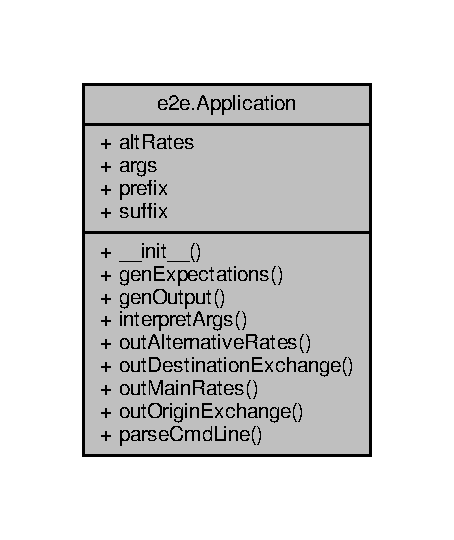
\includegraphics[width=218pt]{classe2e_1_1_application__coll__graph}
\end{center}
\end{figure}
\subsection*{Public Member Functions}
\begin{DoxyCompactItemize}
\item 
def \hyperlink{classe2e_1_1_application_a2267bd2e8d3114095e6271aed7f8c8c9}{\+\_\+\+\_\+init\+\_\+\+\_\+} (self)
\item 
def \hyperlink{classe2e_1_1_application_a72b854da6d69dbcb5031f24dccf9cc71}{gen\+Expectations} (self)
\item 
def \hyperlink{classe2e_1_1_application_a0f753699fabab3ae17407b36404d3b64}{gen\+Output} (self)
\item 
def \hyperlink{classe2e_1_1_application_ae7bc7b58f19d681635cfa8ae06d9769b}{get\+Parameters} (self)
\item 
def \hyperlink{classe2e_1_1_application_ae7b9559aa388f8178300fb4d7a9f9257}{interpret\+Args} (self)
\item 
def \hyperlink{classe2e_1_1_application_acd7798aa633d75001b6f6fde556b8a51}{out\+All\+Rates} (self)
\item 
def \hyperlink{classe2e_1_1_application_a1b099bee6f8170c4c52e7ae884d95b27}{out\+Destination\+Exchange} (self)
\item 
def \hyperlink{classe2e_1_1_application_a3e33fd00d85637393d48ea3f7dbd95c7}{out\+Main\+Rates} (self)
\item 
def \hyperlink{classe2e_1_1_application_adfad90d64cddb8d751961202264ca489}{out\+Origin\+Exchange} (self)
\item 
def \hyperlink{classe2e_1_1_application_a91b8b6df6456d27bed503849ffcdcc77}{parse\+Cmd\+Line} (self)
\end{DoxyCompactItemize}
\subsection*{Public Attributes}
\begin{DoxyCompactItemize}
\item 
\hyperlink{classe2e_1_1_application_abade6fc2e2c04ddd7e48137a2a7721bd}{args}
\item 
\hyperlink{classe2e_1_1_application_a57206c6ccc86c2659edfd8d73d2029f3}{params}
\item 
\hyperlink{classe2e_1_1_application_a027ff25e5409ae17584978a09fc2611a}{prefix}
\item 
\hyperlink{classe2e_1_1_application_a4d824ad36b051d2d629edb314385df0d}{suffix}
\end{DoxyCompactItemize}


\subsection{Detailed Description}


Definition at line \hyperlink{e2e_8py_source_l00133}{133} of file \hyperlink{e2e_8py_source}{e2e.\+py}.



\subsection{Constructor \& Destructor Documentation}
\mbox{\Hypertarget{classe2e_1_1_application_a2267bd2e8d3114095e6271aed7f8c8c9}\label{classe2e_1_1_application_a2267bd2e8d3114095e6271aed7f8c8c9}} 
\index{e2e\+::\+Application@{e2e\+::\+Application}!\+\_\+\+\_\+init\+\_\+\+\_\+@{\+\_\+\+\_\+init\+\_\+\+\_\+}}
\index{\+\_\+\+\_\+init\+\_\+\+\_\+@{\+\_\+\+\_\+init\+\_\+\+\_\+}!e2e\+::\+Application@{e2e\+::\+Application}}
\subsubsection{\texorpdfstring{\+\_\+\+\_\+init\+\_\+\+\_\+()}{\_\_init\_\_()}}
{\footnotesize\ttfamily def e2e.\+Application.\+\_\+\+\_\+init\+\_\+\+\_\+ (\begin{DoxyParamCaption}\item[{}]{self }\end{DoxyParamCaption})}



Definition at line \hyperlink{e2e_8py_source_l00134}{134} of file \hyperlink{e2e_8py_source}{e2e.\+py}.


\begin{DoxyCode}
00134     \textcolor{keyword}{def }\hyperlink{namespacestart__time_a9c9bd378729a13c96a22c8b079ea172c}{\_\_init\_\_} (self):
00135         d = start\_time.getDatetime ()
00136         self.suffix = d.strftime (\textcolor{stringliteral}{'%Y%m%d\_%H%M'})
00137         self.prefix = \textcolor{stringliteral}{'e2e'}
00138         self.params = \textcolor{keywordtype}{None}
00139     
\end{DoxyCode}


\subsection{Member Function Documentation}
\mbox{\Hypertarget{classe2e_1_1_application_a72b854da6d69dbcb5031f24dccf9cc71}\label{classe2e_1_1_application_a72b854da6d69dbcb5031f24dccf9cc71}} 
\index{e2e\+::\+Application@{e2e\+::\+Application}!gen\+Expectations@{gen\+Expectations}}
\index{gen\+Expectations@{gen\+Expectations}!e2e\+::\+Application@{e2e\+::\+Application}}
\subsubsection{\texorpdfstring{gen\+Expectations()}{genExpectations()}}
{\footnotesize\ttfamily def e2e.\+Application.\+gen\+Expectations (\begin{DoxyParamCaption}\item[{}]{self }\end{DoxyParamCaption})}



Definition at line \hyperlink{e2e_8py_source_l00487}{487} of file \hyperlink{e2e_8py_source}{e2e.\+py}.



References \hyperlink{e2e_8py_source_l00386}{e2e.\+Application.\+get\+Parameters()}.


\begin{DoxyCode}
00487     \textcolor{keyword}{def }genExpectations (self):
00488         params = self.getParameters ()
00489 
00490         \textcolor{comment}{# Create the difference}
00491         origin      = params.getOrigin ()
00492         orgTicker   = origin.mkTicker ()
00493         destination = params.getDestination ()
00494         dstTicker   = destination.mkTicker ()
00495         mainRates   = params.getMainRates ()
00496         
00497         diff = \hyperlink{classexchange_1_1_diff_tracker}{exchange.DiffTracker} (mainRates, dstTicker, orgTicker)
00498        
00499         \textcolor{comment}{# Generate the difference}
00500         diff.calc ()
00501         
00502         \textcolor{comment}{# TODO output the formatted difference report}
00503         outFile = params.getRepConclusionOutput ()
00504         line = str (diff) + \textcolor{stringliteral}{"\(\backslash\)n"}
00505         outFile.write (line)
00506         
00507         outFile.close ()
00508         
00509         \textcolor{comment}{# TODO output the JSON differene report}
00510         outFile = params.getJsonConclusionOutput ()
00511         line = diff.dumps () + \textcolor{stringliteral}{"\(\backslash\)n"}
00512         outFile.write (line)
00513         
00514         outFile.close ()
00515             
\end{DoxyCode}
Here is the call graph for this function\+:
\nopagebreak
\begin{figure}[H]
\begin{center}
\leavevmode
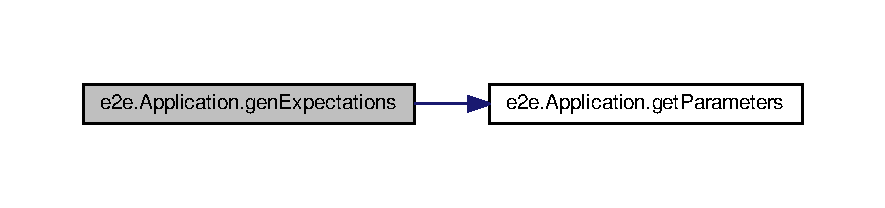
\includegraphics[width=350pt]{classe2e_1_1_application_a72b854da6d69dbcb5031f24dccf9cc71_cgraph}
\end{center}
\end{figure}
\mbox{\Hypertarget{classe2e_1_1_application_a0f753699fabab3ae17407b36404d3b64}\label{classe2e_1_1_application_a0f753699fabab3ae17407b36404d3b64}} 
\index{e2e\+::\+Application@{e2e\+::\+Application}!gen\+Output@{gen\+Output}}
\index{gen\+Output@{gen\+Output}!e2e\+::\+Application@{e2e\+::\+Application}}
\subsubsection{\texorpdfstring{gen\+Output()}{genOutput()}}
{\footnotesize\ttfamily def e2e.\+Application.\+gen\+Output (\begin{DoxyParamCaption}\item[{}]{self }\end{DoxyParamCaption})}



Definition at line \hyperlink{e2e_8py_source_l00516}{516} of file \hyperlink{e2e_8py_source}{e2e.\+py}.


\begin{DoxyCode}
00516     \textcolor{keyword}{def }genOutput (self):
00517         \textcolor{keywordflow}{pass}
00518 
\end{DoxyCode}
\mbox{\Hypertarget{classe2e_1_1_application_ae7bc7b58f19d681635cfa8ae06d9769b}\label{classe2e_1_1_application_ae7bc7b58f19d681635cfa8ae06d9769b}} 
\index{e2e\+::\+Application@{e2e\+::\+Application}!get\+Parameters@{get\+Parameters}}
\index{get\+Parameters@{get\+Parameters}!e2e\+::\+Application@{e2e\+::\+Application}}
\subsubsection{\texorpdfstring{get\+Parameters()}{getParameters()}}
{\footnotesize\ttfamily def e2e.\+Application.\+get\+Parameters (\begin{DoxyParamCaption}\item[{}]{self }\end{DoxyParamCaption})}



Definition at line \hyperlink{e2e_8py_source_l00386}{386} of file \hyperlink{e2e_8py_source}{e2e.\+py}.



References \hyperlink{e2e_8py_source_l00138}{e2e.\+Application.\+params}.



Referenced by \hyperlink{e2e_8py_source_l00487}{e2e.\+Application.\+gen\+Expectations()}, \hyperlink{e2e_8py_source_l00398}{e2e.\+Application.\+out\+All\+Rates()}, \hyperlink{e2e_8py_source_l00452}{e2e.\+Application.\+out\+Destination\+Exchange()}, \hyperlink{e2e_8py_source_l00389}{e2e.\+Application.\+out\+Main\+Rates()}, and \hyperlink{e2e_8py_source_l00417}{e2e.\+Application.\+out\+Origin\+Exchange()}.


\begin{DoxyCode}
00386     \textcolor{keyword}{def }getParameters (self): 
00387         \textcolor{keywordflow}{return} self.params
00388             
\end{DoxyCode}
Here is the caller graph for this function\+:
\nopagebreak
\begin{figure}[H]
\begin{center}
\leavevmode
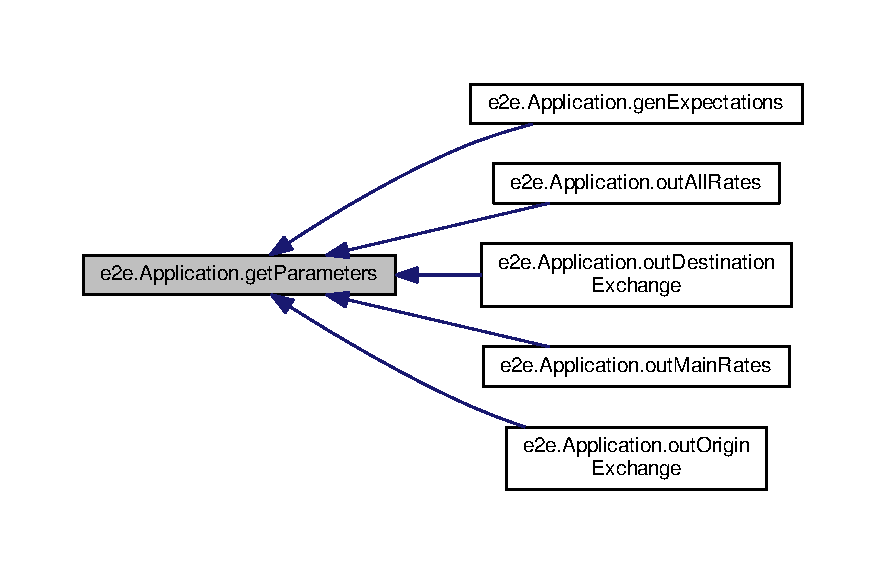
\includegraphics[width=350pt]{classe2e_1_1_application_ae7bc7b58f19d681635cfa8ae06d9769b_icgraph}
\end{center}
\end{figure}
\mbox{\Hypertarget{classe2e_1_1_application_ae7b9559aa388f8178300fb4d7a9f9257}\label{classe2e_1_1_application_ae7b9559aa388f8178300fb4d7a9f9257}} 
\index{e2e\+::\+Application@{e2e\+::\+Application}!interpret\+Args@{interpret\+Args}}
\index{interpret\+Args@{interpret\+Args}!e2e\+::\+Application@{e2e\+::\+Application}}
\subsubsection{\texorpdfstring{interpret\+Args()}{interpretArgs()}}
{\footnotesize\ttfamily def e2e.\+Application.\+interpret\+Args (\begin{DoxyParamCaption}\item[{}]{self }\end{DoxyParamCaption})}



Definition at line \hyperlink{e2e_8py_source_l00183}{183} of file \hyperlink{e2e_8py_source}{e2e.\+py}.



References \hyperlink{e2e_8py_source_l00178}{e2e.\+Application.\+args}, \hyperlink{e2e_8py_source_l00138}{e2e.\+Application.\+params}, \hyperlink{e2e_8py_source_l00137}{e2e.\+Application.\+prefix}, and \hyperlink{e2e_8py_source_l00136}{e2e.\+Application.\+suffix}.


\begin{DoxyCode}
00183     \textcolor{keyword}{def }interpretArgs (self):
00184         result = Parameters ()
00185         
00186 \textcolor{comment}{#        # Open summary file}
00187 \textcolor{comment}{#        if self.args.summary == None:}
00188 \textcolor{comment}{#            try:}
00189 \textcolor{comment}{#                sum\_nam =  self.prefix + '\_' + self.suffix + '.sum'}
00190 \textcolor{comment}{#                sum\_f = open (sum\_nam, 'w')}
00191 \textcolor{comment}{#                }
00192 \textcolor{comment}{#            except IOError:}
00193 \textcolor{comment}{#                # TODO an application specific msg here}
00194 \textcolor{comment}{#                raise}
00195 \textcolor{comment}{#        else:}
00196 \textcolor{comment}{#            sum\_f = sys.\_\_stdout\_\_}
00197 \textcolor{comment}{#            }
00198 \textcolor{comment}{#        result.setSummaryOutput (sum\_f)}
00199 \textcolor{comment}{#            }
00200 \textcolor{comment}{#        # TODO Open output files for destination exchange}
00201 \textcolor{comment}{#        try:}
00202 \textcolor{comment}{#            cnc\_nam  =  self.prefix + '\_conclusion'}
00203 \textcolor{comment}{#            cnc\_nam += '\_' + self.suffix + '.json'}
00204 \textcolor{comment}{#            cnc\_f = open (cnc\_nam, 'w')}
00205 \textcolor{comment}{#            }
00206 \textcolor{comment}{#        except IOError:}
00207 \textcolor{comment}{#            # TODO an application specific msg here}
00208 \textcolor{comment}{#            raise}
00209 \textcolor{comment}{#            }
00210 \textcolor{comment}{#        result.setConclusionOutput (cnc\_f)}
00211             
00212         \textcolor{comment}{# TODO confirm that destinatian and origin exchanges are not equal}
00213         args = self.args 
00214         \textcolor{keywordflow}{if} args.origin == args.destination:
00215             fmt = \textcolor{stringliteral}{'ERROR: Origin exchange \{0\} equal to destination \{1\}'}
00216             msg = fmt.format (args.origin, args.destination)
00217             \textcolor{keywordflow}{raise} Exception (msg)
00218 
00219         \textcolor{comment}{# TODO get exchange names }
00220         gfExchange = \hyperlink{classgen__factory_1_1_gen_factory}{gen\_factory.GenFactory} (
      \hyperlink{classexchange_1_1_exchange}{exchange.Exchange})
00221         exchNames = gfExchange.validClassNames ()
00222         
00223         \textcolor{comment}{# TODO validate destination exchange}
00224         \textcolor{keywordflow}{if} \textcolor{keywordflow}{not} gfExchange.isValidClassName (args.destination):
00225             fmt  = \textcolor{stringliteral}{'ERROR: Destination exchange \{0\} is not a valid '}
00226             fmt += \textcolor{stringliteral}{'exchange name.\(\backslash\)n'}
00227             fmt += \textcolor{stringliteral}{'\(\backslash\)tShould be one of \{1\}'}
00228             msg = fmt.format (args.destination, exchNames)
00229             \textcolor{keywordflow}{raise} Exception (msg)
00230             
00231         \textcolor{comment}{# TODO validate origin exchange}
00232         \textcolor{keywordflow}{if} \textcolor{keywordflow}{not} gfExchange.isValidClassName (args.origin):
00233             fmt  = \textcolor{stringliteral}{'ERROR: Origin exchange \{0\} is not a valid exchange name.\(\backslash\)n'}
00234             fmt += \textcolor{stringliteral}{'\(\backslash\)tShould be one of \{1\}'}
00235             msg = fmt.format (args.origin, exchNames)
00236             \textcolor{keywordflow}{raise} Exception (msg)
00237         
00238         \textcolor{comment}{# TODO open connection with destination exchange}
00239         dstExchange = gfExchange.genObject (args.destination)
00240         result.setDestination (dstExchange)
00241             
00242         \textcolor{comment}{# TODO Open output files for destination exchange}
00243         \textcolor{keywordflow}{try}:
00244             dst\_nam  =  self.prefix + \textcolor{stringliteral}{'\_'} + dstExchange.get\_exch\_prefix ()
00245             dst\_nam += \textcolor{stringliteral}{'\_'} + self.suffix + \textcolor{stringliteral}{'.json'}
00246             e2e\_dst\_f = open (dst\_nam, \textcolor{stringliteral}{'w'})
00247             
00248         \textcolor{keywordflow}{except} IOError:
00249             \textcolor{comment}{# TODO an application specific msg here}
00250             \textcolor{keywordflow}{raise}
00251             
00252         result.setDestinationOutput (e2e\_dst\_f)
00253             
00254         \textcolor{keywordflow}{try}:
00255             dst\_nam  = dstExchange.get\_exch\_prefix ()
00256             dst\_nam += \textcolor{stringliteral}{'\_'} + self.suffix + \textcolor{stringliteral}{'.json'}
00257             dst\_f = open (dst\_nam, \textcolor{stringliteral}{'w'})
00258             
00259         \textcolor{keywordflow}{except} IOError:
00260             \textcolor{comment}{# TODO an application specific msg here}
00261             \textcolor{keywordflow}{raise}
00262             
00263         result.setRawDestinationOutput (dst\_f)
00264             
00265         \textcolor{comment}{# TODO open connection with origin exchange}
00266         orgExchange = gfExchange.genObject (args.origin)
00267         result.setOrigin (orgExchange)
00268             
00269         \textcolor{comment}{# TODO Open output files for origin exchange}
00270         \textcolor{keywordflow}{try}:
00271             org\_nam  =  self.prefix + \textcolor{stringliteral}{'\_'} + orgExchange.get\_exch\_prefix ()
00272             org\_nam += \textcolor{stringliteral}{'\_'} + self.suffix + \textcolor{stringliteral}{'.json'}
00273             e2e\_org\_f = open (org\_nam, \textcolor{stringliteral}{'w'})
00274             
00275         \textcolor{keywordflow}{except} IOError:
00276             \textcolor{comment}{# TODO an application specific2 msg here}
00277             \textcolor{keywordflow}{raise}
00278 
00279         result.setOriginOutput (e2e\_org\_f)
00280             
00281         \textcolor{keywordflow}{try}:
00282             org\_nam  = orgExchange.get\_exch\_prefix ()
00283             org\_nam += \textcolor{stringliteral}{'\_'} + self.suffix + \textcolor{stringliteral}{'.json'}
00284             org\_f = open (org\_nam, \textcolor{stringliteral}{'w'})
00285             
00286         \textcolor{keywordflow}{except} IOError:
00287             \textcolor{comment}{# TODO an application specific msg here}
00288             \textcolor{keywordflow}{raise}
00289             
00290         result.setRawOriginOutput (org\_f)
00291             
00292         \textcolor{comment}{# TODO open connection with main rate service}
00293         gfRates = \hyperlink{classgen__factory_1_1_gen_factory}{gen\_factory.GenFactory} (\hyperlink{classrates_1_1_rates}{rates.Rates})
00294         rates\_names = gfRates.validClassNames ()
00295 
00296         \textcolor{comment}{# TODO validate main rate service}
00297         \textcolor{keywordflow}{if} \textcolor{keywordflow}{not} gfRates.isValidClassName (args.mainRates):
00298             fmt  = \textcolor{stringliteral}{'ERROR: Main rates service \{0\} '}
00299             fmt += \textcolor{stringliteral}{'is not a valid rates name.\(\backslash\)n'}
00300             fmt += \textcolor{stringliteral}{'\(\backslash\)tShould be one of \{1\}'}
00301             msg = fmt.format (args.mainRates, rates\_names)
00302             \textcolor{keywordflow}{raise} Exception (msg)
00303 
00304         mainRates = gfRates.genObject (args.mainRates)
00305         result.setMainRates (mainRates)
00306         
00307         \textcolor{comment}{# TODO Open output file for main rate service}
00308         \textcolor{keywordflow}{try}:
00309             rat\_nam  =  mainRates.getServicePrefix () + \textcolor{stringliteral}{'\_'}
00310             rat\_nam +=  self.suffix + \textcolor{stringliteral}{'.rat'}
00311             rat\_f = open (rat\_nam, \textcolor{stringliteral}{'w'})
00312             
00313         \textcolor{keywordflow}{except} IOError:
00314             \textcolor{comment}{# TODO an application specific msg here}
00315             \textcolor{keywordflow}{raise}        
00316 
00317         result.setMainRatesOutput (rat\_f)
00318             
00319         \textcolor{comment}{# TODO open connections with auxiliary rate services}
00320         allRatesNames = []        
00321         \textcolor{keywordflow}{for} rateName \textcolor{keywordflow}{in} rates\_names:
00322 \textcolor{comment}{#            if rateName == args.mainRates:}
00323 \textcolor{comment}{#                continue }
00324             
00325             allRatesNames.append (rateName)
00326 
00327         result.allRates = []            
00328         \textcolor{keywordflow}{for} rateName \textcolor{keywordflow}{in} allRatesNames:
00329             result.allRates.append (gfRates.genObject (rateName))
00330             
00331         \textcolor{keywordflow}{try}:
00332             allrat\_nam  =  \textcolor{stringliteral}{'all\_rates'} + \textcolor{stringliteral}{'\_'}
00333             allrat\_nam +=  self.suffix + \textcolor{stringliteral}{'.rat'}
00334             allrat\_f = open (allrat\_nam, \textcolor{stringliteral}{'w'})
00335             
00336         \textcolor{keywordflow}{except} IOError:
00337             \textcolor{comment}{# TODO an application specific msg here}
00338             \textcolor{keywordflow}{raise}        
00339 
00340         result.setAllRatesOutput (allrat\_f)
00341             
00342         \textcolor{keywordflow}{try}:
00343             conc\_nam  = \textcolor{stringliteral}{'conc\_'} + orgExchange.get\_exch\_prefix ()
00344             conc\_nam += \textcolor{stringliteral}{'\_'} + dstExchange.get\_exch\_prefix () + \textcolor{stringliteral}{'\_'} 
00345             conc\_nam += self.suffix + \textcolor{stringliteral}{'.rep'}
00346             conc\_f    = open (conc\_nam, \textcolor{stringliteral}{'w'})
00347             
00348         \textcolor{keywordflow}{except} IOError:
00349             \textcolor{comment}{# TODO an application specific msg here}
00350             \textcolor{keywordflow}{raise}        
00351 
00352         result.setRepConclusionOutput (conc\_f)
00353             
00354         \textcolor{keywordflow}{try}:
00355             conc\_nam  = \textcolor{stringliteral}{'conc\_'} + orgExchange.get\_exch\_prefix ()
00356             conc\_nam += \textcolor{stringliteral}{'\_'} + dstExchange.get\_exch\_prefix () + \textcolor{stringliteral}{'\_'} 
00357             conc\_nam += self.suffix + \textcolor{stringliteral}{'.json'}
00358             conc\_f    = open (conc\_nam, \textcolor{stringliteral}{'w'})
00359             
00360         \textcolor{keywordflow}{except} IOError:
00361             \textcolor{comment}{# TODO an application specific msg here}
00362             \textcolor{keywordflow}{raise}        
00363 
00364         result.setJsonConclusionOutput (conc\_f)
00365         
00366         self.params = result
00367         
00368         args = self.args                
00369         \textcolor{keywordflow}{if} args.verbose:
00370             repFile = result.getRepConclusionOutput ()
00371                         
00372             
00373             lines = [\textcolor{stringliteral}{''}, \textcolor{stringliteral}{''}, \textcolor{stringliteral}{''}, \textcolor{stringliteral}{''}, \textcolor{stringliteral}{''}]
00374             lines[0] = \textcolor{stringliteral}{'Verbose output enabled\(\backslash\)n'}
00375             lines[1] = \textcolor{stringliteral}{'Main rate service: \{0\}'}.format (args.mainRates)
00376             lines[2] = \textcolor{stringliteral}{'Exchanges'}
00377             lines[3] = \textcolor{stringliteral}{'Origin:            \{0\}'}.format (args.origin)
00378             lines[4] = \textcolor{stringliteral}{'Destination:       \{0\}\(\backslash\)n'}.format (args.destination)
00379 
00380             \textcolor{keywordflow}{for} line \textcolor{keywordflow}{in} lines:
00381                 repFile.write (line + \textcolor{stringliteral}{'\(\backslash\)n'})
00382             
00383         \textcolor{comment}{# Normal function termination }
00384         \textcolor{keywordflow}{return} result 
00385         
\end{DoxyCode}
\mbox{\Hypertarget{classe2e_1_1_application_acd7798aa633d75001b6f6fde556b8a51}\label{classe2e_1_1_application_acd7798aa633d75001b6f6fde556b8a51}} 
\index{e2e\+::\+Application@{e2e\+::\+Application}!out\+All\+Rates@{out\+All\+Rates}}
\index{out\+All\+Rates@{out\+All\+Rates}!e2e\+::\+Application@{e2e\+::\+Application}}
\subsubsection{\texorpdfstring{out\+All\+Rates()}{outAllRates()}}
{\footnotesize\ttfamily def e2e.\+Application.\+out\+All\+Rates (\begin{DoxyParamCaption}\item[{}]{self }\end{DoxyParamCaption})}



Definition at line \hyperlink{e2e_8py_source_l00398}{398} of file \hyperlink{e2e_8py_source}{e2e.\+py}.



References \hyperlink{e2e_8py_source_l00386}{e2e.\+Application.\+get\+Parameters()}.


\begin{DoxyCode}
00398     \textcolor{keyword}{def }outAllRates (self):
00399         \textcolor{comment}{# TODO calculate average rate and individual differences}
00400         params = self.getParameters ()
00401         allRates = params.getAllRates ()
00402         outFile = params.getAllRatesOutput ()
00403         repFile = params.getRepConclusionOutput ()
00404         
00405         repFile.write (\textcolor{stringliteral}{"\(\backslash\)nExchange services\(\backslash\)n"}) 
00406         
00407         \textcolor{keywordflow}{for} theseRates \textcolor{keywordflow}{in} allRates:
00408             line = str (theseRates) + \textcolor{stringliteral}{"\(\backslash\)n"}
00409             outFile.write (line)
00410             repFile.write (line)
00411 
00412         repFile.write (\textcolor{stringliteral}{'\(\backslash\)n'})
00413         
00414         outFile.close ()
00415         repFile.flush ()
00416     
\end{DoxyCode}
Here is the call graph for this function\+:
\nopagebreak
\begin{figure}[H]
\begin{center}
\leavevmode
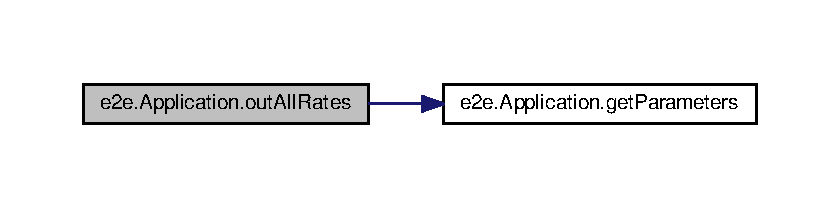
\includegraphics[width=350pt]{classe2e_1_1_application_acd7798aa633d75001b6f6fde556b8a51_cgraph}
\end{center}
\end{figure}
\mbox{\Hypertarget{classe2e_1_1_application_a1b099bee6f8170c4c52e7ae884d95b27}\label{classe2e_1_1_application_a1b099bee6f8170c4c52e7ae884d95b27}} 
\index{e2e\+::\+Application@{e2e\+::\+Application}!out\+Destination\+Exchange@{out\+Destination\+Exchange}}
\index{out\+Destination\+Exchange@{out\+Destination\+Exchange}!e2e\+::\+Application@{e2e\+::\+Application}}
\subsubsection{\texorpdfstring{out\+Destination\+Exchange()}{outDestinationExchange()}}
{\footnotesize\ttfamily def e2e.\+Application.\+out\+Destination\+Exchange (\begin{DoxyParamCaption}\item[{}]{self }\end{DoxyParamCaption})}



Definition at line \hyperlink{e2e_8py_source_l00452}{452} of file \hyperlink{e2e_8py_source}{e2e.\+py}.



References \hyperlink{e2e_8py_source_l00386}{e2e.\+Application.\+get\+Parameters()}.


\begin{DoxyCode}
00452     \textcolor{keyword}{def }outDestinationExchange (self):
00453         params = self.getParameters ()
00454         
00455         \textcolor{comment}{# Get origin exchange data}
00456         destination = params.getDestination ()
00457         destination.get\_ticker ()
00458         ticker = destination.mkTicker ()
00459 
00460         \textcolor{comment}{# Output raw exchange data}
00461         outFile = params.getRawDestinationOutput ()
00462         line = str (destination.getOriginalTicker ()) + \textcolor{stringliteral}{"\(\backslash\)n"}
00463         outFile.write (line)
00464         
00465         outFile.close ()
00466     
00467         \textcolor{comment}{# Output e2e exchange data}
00468         outFile = params.getDestinationOutput ()
00469         line = str (ticker.dumps ()) + \textcolor{stringliteral}{"\(\backslash\)n"}
00470         outFile.write (line)
00471         
00472         outFile.close ()
00473         
00474         \textcolor{comment}{# TODO output origin data as report}
00475         repFile = params.getRepConclusionOutput ()
00476         line = \textcolor{stringliteral}{"\(\backslash\)nDestination exchange"}
00477         repFile.write (line + \textcolor{stringliteral}{'\(\backslash\)n'})
00478         
00479         line = str (ticker) + \textcolor{stringliteral}{"\(\backslash\)n"}
00480         repFile.write (line)
00481         
00482         repFile.flush ()
00483     
00484         \textcolor{comment}{# Normal function termination }
00485         \textcolor{keywordflow}{return} 
00486     
\end{DoxyCode}
Here is the call graph for this function\+:
\nopagebreak
\begin{figure}[H]
\begin{center}
\leavevmode
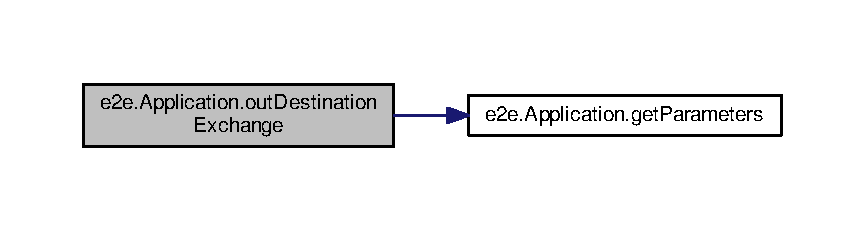
\includegraphics[width=350pt]{classe2e_1_1_application_a1b099bee6f8170c4c52e7ae884d95b27_cgraph}
\end{center}
\end{figure}
\mbox{\Hypertarget{classe2e_1_1_application_a3e33fd00d85637393d48ea3f7dbd95c7}\label{classe2e_1_1_application_a3e33fd00d85637393d48ea3f7dbd95c7}} 
\index{e2e\+::\+Application@{e2e\+::\+Application}!out\+Main\+Rates@{out\+Main\+Rates}}
\index{out\+Main\+Rates@{out\+Main\+Rates}!e2e\+::\+Application@{e2e\+::\+Application}}
\subsubsection{\texorpdfstring{out\+Main\+Rates()}{outMainRates()}}
{\footnotesize\ttfamily def e2e.\+Application.\+out\+Main\+Rates (\begin{DoxyParamCaption}\item[{}]{self }\end{DoxyParamCaption})}



Definition at line \hyperlink{e2e_8py_source_l00389}{389} of file \hyperlink{e2e_8py_source}{e2e.\+py}.



References \hyperlink{e2e_8py_source_l00386}{e2e.\+Application.\+get\+Parameters()}.


\begin{DoxyCode}
00389     \textcolor{keyword}{def }outMainRates (self):
00390         params = self.getParameters ()
00391         mainRates = params.getMainRates ()
00392         outFile = params.getMainRatesOutput ()
00393         line = str (mainRates) + \textcolor{stringliteral}{"\(\backslash\)n"}
00394         outFile.write (line)
00395         
00396         outFile.close ()
00397     
\end{DoxyCode}
Here is the call graph for this function\+:
\nopagebreak
\begin{figure}[H]
\begin{center}
\leavevmode
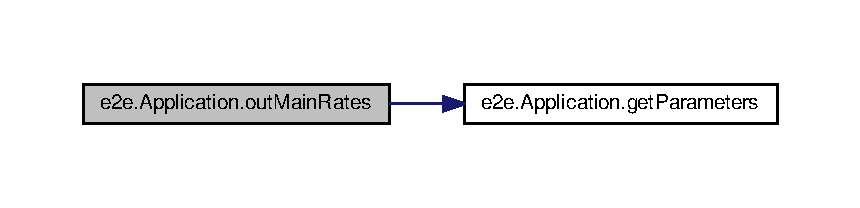
\includegraphics[width=350pt]{classe2e_1_1_application_a3e33fd00d85637393d48ea3f7dbd95c7_cgraph}
\end{center}
\end{figure}
\mbox{\Hypertarget{classe2e_1_1_application_adfad90d64cddb8d751961202264ca489}\label{classe2e_1_1_application_adfad90d64cddb8d751961202264ca489}} 
\index{e2e\+::\+Application@{e2e\+::\+Application}!out\+Origin\+Exchange@{out\+Origin\+Exchange}}
\index{out\+Origin\+Exchange@{out\+Origin\+Exchange}!e2e\+::\+Application@{e2e\+::\+Application}}
\subsubsection{\texorpdfstring{out\+Origin\+Exchange()}{outOriginExchange()}}
{\footnotesize\ttfamily def e2e.\+Application.\+out\+Origin\+Exchange (\begin{DoxyParamCaption}\item[{}]{self }\end{DoxyParamCaption})}



Definition at line \hyperlink{e2e_8py_source_l00417}{417} of file \hyperlink{e2e_8py_source}{e2e.\+py}.



References \hyperlink{e2e_8py_source_l00386}{e2e.\+Application.\+get\+Parameters()}.


\begin{DoxyCode}
00417     \textcolor{keyword}{def }outOriginExchange (self):
00418         params = self.getParameters ()
00419         
00420         \textcolor{comment}{# Get origin exchange data}
00421         origin = params.getOrigin ()
00422         origin.get\_ticker ()
00423         ticker = origin.mkTicker ()
00424 
00425         \textcolor{comment}{# Output raw origin exchange data}
00426         outFile = params.getRawOriginOutput ()
00427         line = str (origin.getOriginalTicker ()) + \textcolor{stringliteral}{"\(\backslash\)n"}
00428         outFile.write (line)
00429         
00430         outFile.close ()
00431     
00432         \textcolor{comment}{# Output e2e origin exchange data}
00433         outFile = params.getOriginOutput ()
00434         line = str (ticker.dumps ()) + \textcolor{stringliteral}{"\(\backslash\)n"}
00435         outFile.write (line)
00436         
00437         outFile.close ()
00438         
00439         \textcolor{comment}{# TODO output origin data as report}
00440         repFile = params.getRepConclusionOutput ()
00441         line = \textcolor{stringliteral}{"\(\backslash\)nOrigin exchange"}
00442         repFile.write (line + \textcolor{stringliteral}{'\(\backslash\)n'})
00443         
00444         line = str (ticker) + \textcolor{stringliteral}{"\(\backslash\)n"}
00445         repFile.write (line)
00446         
00447         repFile.flush ()
00448     
00449         \textcolor{comment}{# Normal function termination }
00450         \textcolor{keywordflow}{return} 
00451     
\end{DoxyCode}
Here is the call graph for this function\+:
\nopagebreak
\begin{figure}[H]
\begin{center}
\leavevmode
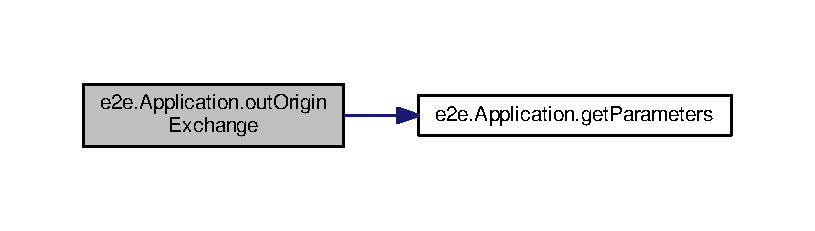
\includegraphics[width=350pt]{classe2e_1_1_application_adfad90d64cddb8d751961202264ca489_cgraph}
\end{center}
\end{figure}
\mbox{\Hypertarget{classe2e_1_1_application_a91b8b6df6456d27bed503849ffcdcc77}\label{classe2e_1_1_application_a91b8b6df6456d27bed503849ffcdcc77}} 
\index{e2e\+::\+Application@{e2e\+::\+Application}!parse\+Cmd\+Line@{parse\+Cmd\+Line}}
\index{parse\+Cmd\+Line@{parse\+Cmd\+Line}!e2e\+::\+Application@{e2e\+::\+Application}}
\subsubsection{\texorpdfstring{parse\+Cmd\+Line()}{parseCmdLine()}}
{\footnotesize\ttfamily def e2e.\+Application.\+parse\+Cmd\+Line (\begin{DoxyParamCaption}\item[{}]{self }\end{DoxyParamCaption})}



Definition at line \hyperlink{e2e_8py_source_l00140}{140} of file \hyperlink{e2e_8py_source}{e2e.\+py}.


\begin{DoxyCode}
00140     \textcolor{keyword}{def }parseCmdLine (self):
00141         desc = \textcolor{stringliteral}{'Compare two exchanges for a round operation'}
00142         parser = argparse.ArgumentParser (description = desc)
00143         
00144 \textcolor{comment}{#        desc = 'Summary report (Default is stdout)' }
00145 \textcolor{comment}{#        parser.add\_argument ('-s', '--summary', required = False,}
00146 \textcolor{comment}{#                             help = desc)}
00147 \textcolor{comment}{#        desc = 'File name for the conclusion of the arbitrage'}
00148 \textcolor{comment}{#        parser.add\_argument ('-c', '--conclusion', required = True,}
00149 \textcolor{comment}{#                             help = desc)}
00150         parser.add\_argument (\textcolor{stringliteral}{'-m'}, \textcolor{stringliteral}{'--main'}, metavar = \textcolor{stringliteral}{"RATES"}, 
00151                              default = \textcolor{stringliteral}{'Google'},
00152                              help = \textcolor{stringliteral}{'Main rate service'})
00153 \textcolor{comment}{#        parser.add\_argument ('-a', '--alternative', metavar = "RATES",}
00154 \textcolor{comment}{#                             default = 'XRates',}
00155 \textcolor{comment}{#                             help = 'Alternative rate service')}
00156         parser.add\_argument (\textcolor{stringliteral}{'-o'}, \textcolor{stringliteral}{'--origin'}, metavar = \textcolor{stringliteral}{"EXCHANGE"},
00157                              required = \textcolor{keyword}{True},
00158                              help = \textcolor{stringliteral}{'Origin exchange'})
00159         parser.add\_argument (\textcolor{stringliteral}{'-d'}, \textcolor{stringliteral}{'--destination'}, metavar = \textcolor{stringliteral}{"EXCHANGE"},
00160                              required = \textcolor{keyword}{True},
00161                              help = \textcolor{stringliteral}{'Destination exchange'})
00162         parser.add\_argument (\textcolor{stringliteral}{'-v'}, \textcolor{stringliteral}{'--verbose'}, action = \textcolor{stringliteral}{"store\_true"},
00163                              help = \textcolor{stringliteral}{'Increase output verbosity'})
00164                              
00165         args = parser.parse\_args ()
00166         
00167         \textcolor{comment}{# TODO complete the copy of cmdline parameters}
00168         
00169         result = Args ()
00170 \textcolor{comment}{#        result.summary     = args.summary }
00171 \textcolor{comment}{#        result.conclusion  = args.conclusion }
00172         result.mainRates   = args.main 
00173 \textcolor{comment}{#        result.altRates    = args.alternative }
00174         result.origin      = args.origin 
00175         result.destination = args.destination 
00176         result.verbose     = args.verbose
00177         
00178         self.args = result
00179         
00180         \textcolor{comment}{# Normal function termination}
00181         \textcolor{keywordflow}{return} result
00182         
\end{DoxyCode}


\subsection{Member Data Documentation}
\mbox{\Hypertarget{classe2e_1_1_application_abade6fc2e2c04ddd7e48137a2a7721bd}\label{classe2e_1_1_application_abade6fc2e2c04ddd7e48137a2a7721bd}} 
\index{e2e\+::\+Application@{e2e\+::\+Application}!args@{args}}
\index{args@{args}!e2e\+::\+Application@{e2e\+::\+Application}}
\subsubsection{\texorpdfstring{args}{args}}
{\footnotesize\ttfamily e2e.\+Application.\+args}



Definition at line \hyperlink{e2e_8py_source_l00178}{178} of file \hyperlink{e2e_8py_source}{e2e.\+py}.



Referenced by \hyperlink{e2e_8py_source_l00183}{e2e.\+Application.\+interpret\+Args()}.

\mbox{\Hypertarget{classe2e_1_1_application_a57206c6ccc86c2659edfd8d73d2029f3}\label{classe2e_1_1_application_a57206c6ccc86c2659edfd8d73d2029f3}} 
\index{e2e\+::\+Application@{e2e\+::\+Application}!params@{params}}
\index{params@{params}!e2e\+::\+Application@{e2e\+::\+Application}}
\subsubsection{\texorpdfstring{params}{params}}
{\footnotesize\ttfamily e2e.\+Application.\+params}



Definition at line \hyperlink{e2e_8py_source_l00138}{138} of file \hyperlink{e2e_8py_source}{e2e.\+py}.



Referenced by \hyperlink{e2e_8py_source_l00386}{e2e.\+Application.\+get\+Parameters()}, and \hyperlink{e2e_8py_source_l00183}{e2e.\+Application.\+interpret\+Args()}.

\mbox{\Hypertarget{classe2e_1_1_application_a027ff25e5409ae17584978a09fc2611a}\label{classe2e_1_1_application_a027ff25e5409ae17584978a09fc2611a}} 
\index{e2e\+::\+Application@{e2e\+::\+Application}!prefix@{prefix}}
\index{prefix@{prefix}!e2e\+::\+Application@{e2e\+::\+Application}}
\subsubsection{\texorpdfstring{prefix}{prefix}}
{\footnotesize\ttfamily e2e.\+Application.\+prefix}



Definition at line \hyperlink{e2e_8py_source_l00137}{137} of file \hyperlink{e2e_8py_source}{e2e.\+py}.



Referenced by \hyperlink{e2e_8py_source_l00183}{e2e.\+Application.\+interpret\+Args()}.

\mbox{\Hypertarget{classe2e_1_1_application_a4d824ad36b051d2d629edb314385df0d}\label{classe2e_1_1_application_a4d824ad36b051d2d629edb314385df0d}} 
\index{e2e\+::\+Application@{e2e\+::\+Application}!suffix@{suffix}}
\index{suffix@{suffix}!e2e\+::\+Application@{e2e\+::\+Application}}
\subsubsection{\texorpdfstring{suffix}{suffix}}
{\footnotesize\ttfamily e2e.\+Application.\+suffix}



Definition at line \hyperlink{e2e_8py_source_l00136}{136} of file \hyperlink{e2e_8py_source}{e2e.\+py}.



Referenced by \hyperlink{e2e_8py_source_l00183}{e2e.\+Application.\+interpret\+Args()}.



The documentation for this class was generated from the following file\+:\begin{DoxyCompactItemize}
\item 
/home/hilton/github/exch2exh/\hyperlink{e2e_8py}{e2e.\+py}\end{DoxyCompactItemize}

\hypertarget{classe2e_1_1_args}{}\section{e2e.\+Args Class Reference}
\label{classe2e_1_1_args}\index{e2e.\+Args@{e2e.\+Args}}


Collaboration diagram for e2e.\+Args\+:\nopagebreak
\begin{figure}[H]
\begin{center}
\leavevmode
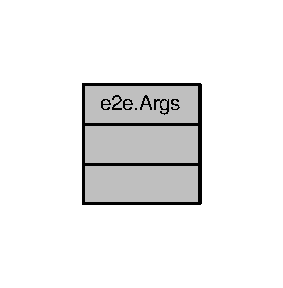
\includegraphics[width=136pt]{classe2e_1_1_args__coll__graph}
\end{center}
\end{figure}


\subsection{Detailed Description}


Definition at line \hyperlink{e2e_8py_source_l00022}{22} of file \hyperlink{e2e_8py_source}{e2e.\+py}.



The documentation for this class was generated from the following file\+:\begin{DoxyCompactItemize}
\item 
/home/hilton/github/exch2exh/\hyperlink{e2e_8py}{e2e.\+py}\end{DoxyCompactItemize}

\hypertarget{classexchange_1_1_datetime_encoder}{}\section{exchange.\+Datetime\+Encoder Class Reference}
\label{classexchange_1_1_datetime_encoder}\index{exchange.\+Datetime\+Encoder@{exchange.\+Datetime\+Encoder}}


Inheritance diagram for exchange.\+Datetime\+Encoder\+:\nopagebreak
\begin{figure}[H]
\begin{center}
\leavevmode
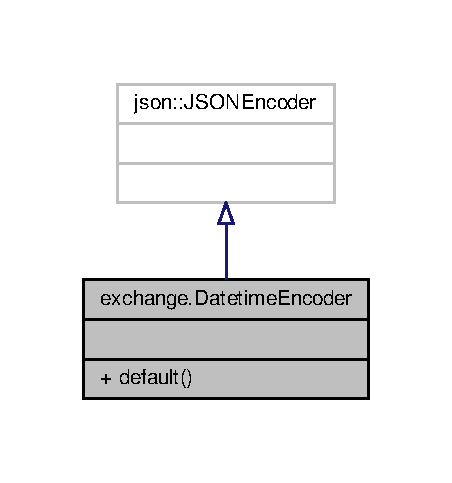
\includegraphics[width=217pt]{classexchange_1_1_datetime_encoder__inherit__graph}
\end{center}
\end{figure}


Collaboration diagram for exchange.\+Datetime\+Encoder\+:\nopagebreak
\begin{figure}[H]
\begin{center}
\leavevmode
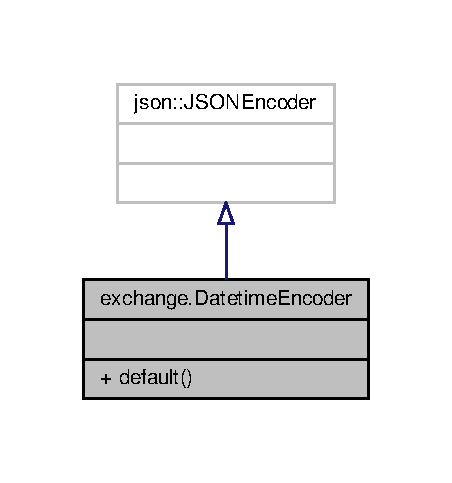
\includegraphics[width=217pt]{classexchange_1_1_datetime_encoder__coll__graph}
\end{center}
\end{figure}
\subsection*{Public Member Functions}
\begin{DoxyCompactItemize}
\item 
def \hyperlink{classexchange_1_1_datetime_encoder_a0bb4f94a13ce6c33e8d68869e282d24f}{default} (self, obj)
\end{DoxyCompactItemize}


\subsection{Detailed Description}


Definition at line \hyperlink{exchange_8py_source_l00028}{28} of file \hyperlink{exchange_8py_source}{exchange.\+py}.



\subsection{Member Function Documentation}
\index{exchange\+::\+Datetime\+Encoder@{exchange\+::\+Datetime\+Encoder}!default@{default}}
\index{default@{default}!exchange\+::\+Datetime\+Encoder@{exchange\+::\+Datetime\+Encoder}}
\subsubsection[{\texorpdfstring{default(self, obj)}{default(self, obj)}}]{\setlength{\rightskip}{0pt plus 5cm}def exchange.\+Datetime\+Encoder.\+default (
\begin{DoxyParamCaption}
\item[{}]{self, }
\item[{}]{obj}
\end{DoxyParamCaption}
)}\hypertarget{classexchange_1_1_datetime_encoder_a0bb4f94a13ce6c33e8d68869e282d24f}{}\label{classexchange_1_1_datetime_encoder_a0bb4f94a13ce6c33e8d68869e282d24f}


Definition at line \hyperlink{exchange_8py_source_l00029}{29} of file \hyperlink{exchange_8py_source}{exchange.\+py}.


\begin{DoxyCode}
\hypertarget{classexchange_1_1_datetime_encoder.tex_l00029}{}\hyperlink{classexchange_1_1_datetime_encoder_a0bb4f94a13ce6c33e8d68869e282d24f}{00029}     \textcolor{keyword}{def }\hyperlink{classexchange_1_1_datetime_encoder_a0bb4f94a13ce6c33e8d68869e282d24f}{default}(self, obj):
00030         \textcolor{keywordflow}{if} isinstance (obj, datetime.datetime):
00031             \textcolor{keywordflow}{return} obj.\_\_repr\_\_ ()
00032             
00033         \textcolor{comment}{# Let the base class default method raise the TypeError}
00034         \textcolor{keywordflow}{return} json.JSONEncoder.default(self, obj)
00035 
00036 \textcolor{comment}{# Standard way of packing oderdebook information across all exchange classes}
00037         
\end{DoxyCode}


The documentation for this class was generated from the following file\+:\begin{DoxyCompactItemize}
\item 
/home/hilton/github/exch2exh/\hyperlink{exchange_8py}{exchange.\+py}\end{DoxyCompactItemize}

\hypertarget{classexch2exch_1_1_differences}{\section{exch2exch.\-Differences Class Reference}
\label{classexch2exch_1_1_differences}\index{exch2exch.\-Differences@{exch2exch.\-Differences}}
}
\subsection*{Public Member Functions}
\begin{DoxyCompactItemize}
\item 
def \hyperlink{classexch2exch_1_1_differences_a233d3aa10e3542a0d8229b299384b2b8}{\-\_\-\-\_\-init\-\_\-\-\_\-}
\item 
def \hyperlink{classexch2exch_1_1_differences_a4dbc60a284d9679bb9682d46112ee1bf}{\-\_\-\-\_\-str\-\_\-\-\_\-}
\item 
def \hyperlink{classexch2exch_1_1_differences_a3083b0bcc349937fb7ad708bc683e3d4}{get\-Max\-Delta}
\item 
def \hyperlink{classexch2exch_1_1_differences_a83359c7999d33257746aa09f653e41fa}{get\-Max\-Gain}
\item 
def \hyperlink{classexch2exch_1_1_differences_ae6156c3361371d1688de9b334ef7dc8d}{get\-Min\-Delta}
\item 
def \hyperlink{classexch2exch_1_1_differences_a3c7fc587dedfda0e303260f244021017}{get\-Min\-Gain}
\end{DoxyCompactItemize}
\subsection*{Public Attributes}
\begin{DoxyCompactItemize}
\item 
\hyperlink{classexch2exch_1_1_differences_a261a74cc25d77b2608898fa5611f9f0b}{dmax}
\item 
\hyperlink{classexch2exch_1_1_differences_a7825bfca16b5775aa770c8810412b215}{dmin}
\item 
\hyperlink{classexch2exch_1_1_differences_a569f2a6fa0e33ad725c3c3ada259ddcc}{gmax}
\item 
\hyperlink{classexch2exch_1_1_differences_a33c9add531b5b46c49ae322657343382}{gmin}
\item 
\hyperlink{classexch2exch_1_1_differences_a81c81e9c15b5ea8a5d39bb99d85250e1}{mb}
\item 
\hyperlink{classexch2exch_1_1_differences_a6de3ee563584c83a97ba815db8ec7831}{ok}
\item 
\hyperlink{classexch2exch_1_1_differences_a64aec2fc7f20028f0bd834908cbea116}{rates}
\end{DoxyCompactItemize}


\subsection{Detailed Description}


Definition at line 100 of file exch2exch.\-py.



\subsection{Constructor \& Destructor Documentation}
\hypertarget{classexch2exch_1_1_differences_a233d3aa10e3542a0d8229b299384b2b8}{\index{exch2exch\-::\-Differences@{exch2exch\-::\-Differences}!\-\_\-\-\_\-init\-\_\-\-\_\-@{\-\_\-\-\_\-init\-\_\-\-\_\-}}
\index{\-\_\-\-\_\-init\-\_\-\-\_\-@{\-\_\-\-\_\-init\-\_\-\-\_\-}!exch2exch::Differences@{exch2exch\-::\-Differences}}
\subsubsection[{\-\_\-\-\_\-init\-\_\-\-\_\-}]{\setlength{\rightskip}{0pt plus 5cm}def exch2exch.\-Differences.\-\_\-\-\_\-init\-\_\-\-\_\- (
\begin{DoxyParamCaption}
\item[{}]{self, }
\item[{}]{rates, }
\item[{}]{mb, }
\item[{}]{ok}
\end{DoxyParamCaption}
)}}\label{classexch2exch_1_1_differences_a233d3aa10e3542a0d8229b299384b2b8}


Definition at line 101 of file exch2exch.\-py.


\begin{DoxyCode}
101 
102     \textcolor{keyword}{def }\hyperlink{classexch2exch_1_1_differences_a233d3aa10e3542a0d8229b299384b2b8}{\_\_init\_\_} (self, rates, mb, ok):
103         self.\hyperlink{classexch2exch_1_1_differences_a64aec2fc7f20028f0bd834908cbea116}{rates} = rates
104         self.\hyperlink{classexch2exch_1_1_differences_a81c81e9c15b5ea8a5d39bb99d85250e1}{mb} = mb
105         self.\hyperlink{classexch2exch_1_1_differences_a6de3ee563584c83a97ba815db8ec7831}{ok} = ok
106         
107         self.\hyperlink{classexch2exch_1_1_differences_a7825bfca16b5775aa770c8810412b215}{dmin} = mb.getLow ()  - ok.getLow ()   
108         self.\hyperlink{classexch2exch_1_1_differences_a261a74cc25d77b2608898fa5611f9f0b}{dmax} = mb.getHigh () - ok.getLow ()
109         
110         self.\hyperlink{classexch2exch_1_1_differences_a33c9add531b5b46c49ae322657343382}{gmin} = 100.0 * self.\hyperlink{classexch2exch_1_1_differences_a7825bfca16b5775aa770c8810412b215}{dmin} / ok.getHigh ()
111         self.\hyperlink{classexch2exch_1_1_differences_a569f2a6fa0e33ad725c3c3ada259ddcc}{gmax} = 100.0 * self.\hyperlink{classexch2exch_1_1_differences_a261a74cc25d77b2608898fa5611f9f0b}{dmax} / ok.getLow ()
        
\end{DoxyCode}


\subsection{Member Function Documentation}
\hypertarget{classexch2exch_1_1_differences_a4dbc60a284d9679bb9682d46112ee1bf}{\index{exch2exch\-::\-Differences@{exch2exch\-::\-Differences}!\-\_\-\-\_\-str\-\_\-\-\_\-@{\-\_\-\-\_\-str\-\_\-\-\_\-}}
\index{\-\_\-\-\_\-str\-\_\-\-\_\-@{\-\_\-\-\_\-str\-\_\-\-\_\-}!exch2exch::Differences@{exch2exch\-::\-Differences}}
\subsubsection[{\-\_\-\-\_\-str\-\_\-\-\_\-}]{\setlength{\rightskip}{0pt plus 5cm}def exch2exch.\-Differences.\-\_\-\-\_\-str\-\_\-\-\_\- (
\begin{DoxyParamCaption}
\item[{}]{self}
\end{DoxyParamCaption}
)}}\label{classexch2exch_1_1_differences_a4dbc60a284d9679bb9682d46112ee1bf}


Definition at line 124 of file exch2exch.\-py.



References exch2exch.\-Differences.\-get\-Max\-Delta(), exch2exch.\-Differences.\-get\-Max\-Gain(), exch2exch.\-Differences.\-get\-Min\-Delta(), and exch2exch.\-Differences.\-get\-Min\-Gain().


\begin{DoxyCode}
124 
125     \textcolor{keyword}{def }\hyperlink{classexch2exch_1_1_differences_a4dbc60a284d9679bb9682d46112ee1bf}{\_\_str\_\_} (self):
126         result = \textcolor{stringliteral}{""}
127         
128         oname = self.ok.getExchangeName ()
129         mname = self.ok.getExchangeName ()
130         sname = self.rates.getServiceName ()
131         
132         fmt = \textcolor{stringliteral}{"Calculation between \{0\} and \{1\} rates, with conversion from \{2\}"}
133         result = fmt.format (oname, mname, sname)
134         
135         \textcolor{comment}{# TODO create evaluation for 24h and for the most recent sell/buy}
136         
137         fmt = \textcolor{stringliteral}{"\(\backslash\)nLast: minimum \{0:.4f\}, maximum \{1:.4f\}"}
138         result += fmt.format (self.\hyperlink{classexch2exch_1_1_differences_ae6156c3361371d1688de9b334ef7dc8d}{getMinDelta} (), self.\hyperlink{classexch2exch_1_1_differences_a3083b0bcc349937fb7ad708bc683e3d4}{getMaxDelta} ())
139         
140         fmt = \textcolor{stringliteral}{"\(\backslash\)nGain: minimum \{0:.4f\} %, maximum \{1:.4f\} %"}
141         result += fmt.format (self.\hyperlink{classexch2exch_1_1_differences_a3c7fc587dedfda0e303260f244021017}{getMinGain} (), self.\hyperlink{classexch2exch_1_1_differences_a83359c7999d33257746aa09f653e41fa}{getMaxGain} ())
142         
143         \textcolor{keywordflow}{return} result
144 
145 \textcolor{comment}{#        }
146 \textcolor{comment}{# }
147 \textcolor{comment}{# Google section }
148 \textcolor{comment}{#}

\end{DoxyCode}


Here is the call graph for this function\-:
\nopagebreak
\begin{figure}[H]
\begin{center}
\leavevmode
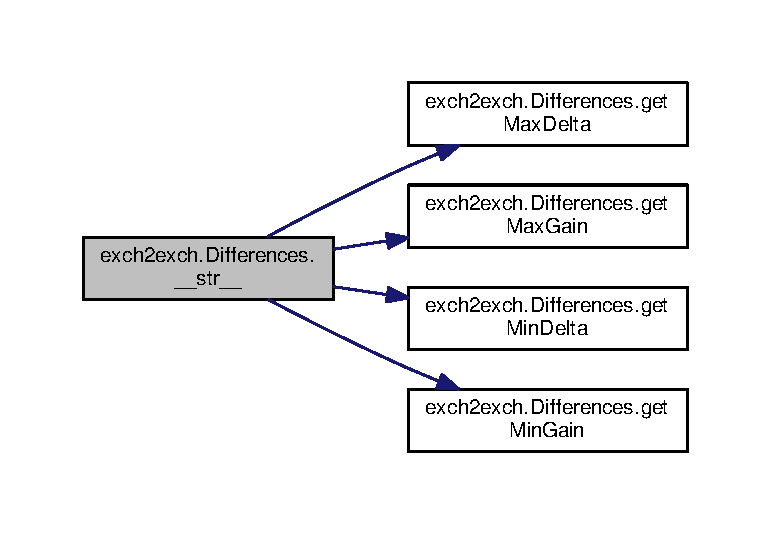
\includegraphics[width=350pt]{classexch2exch_1_1_differences_a4dbc60a284d9679bb9682d46112ee1bf_cgraph}
\end{center}
\end{figure}


\hypertarget{classexch2exch_1_1_differences_a3083b0bcc349937fb7ad708bc683e3d4}{\index{exch2exch\-::\-Differences@{exch2exch\-::\-Differences}!get\-Max\-Delta@{get\-Max\-Delta}}
\index{get\-Max\-Delta@{get\-Max\-Delta}!exch2exch::Differences@{exch2exch\-::\-Differences}}
\subsubsection[{get\-Max\-Delta}]{\setlength{\rightskip}{0pt plus 5cm}def exch2exch.\-Differences.\-get\-Max\-Delta (
\begin{DoxyParamCaption}
\item[{}]{self}
\end{DoxyParamCaption}
)}}\label{classexch2exch_1_1_differences_a3083b0bcc349937fb7ad708bc683e3d4}


Definition at line 115 of file exch2exch.\-py.



References exch2exch.\-Differences.\-dmax.



Referenced by raw\-\_\-urlparser.\-Differences.\-\_\-\-\_\-str\-\_\-\-\_\-(), and exch2exch.\-Differences.\-\_\-\-\_\-str\-\_\-\-\_\-().


\begin{DoxyCode}
115 
116     \textcolor{keyword}{def }\hyperlink{classexch2exch_1_1_differences_a3083b0bcc349937fb7ad708bc683e3d4}{getMaxDelta} (self): 
117         \textcolor{keywordflow}{return} self.\hyperlink{classexch2exch_1_1_differences_a261a74cc25d77b2608898fa5611f9f0b}{dmax}
        
\end{DoxyCode}


Here is the caller graph for this function\-:
\nopagebreak
\begin{figure}[H]
\begin{center}
\leavevmode
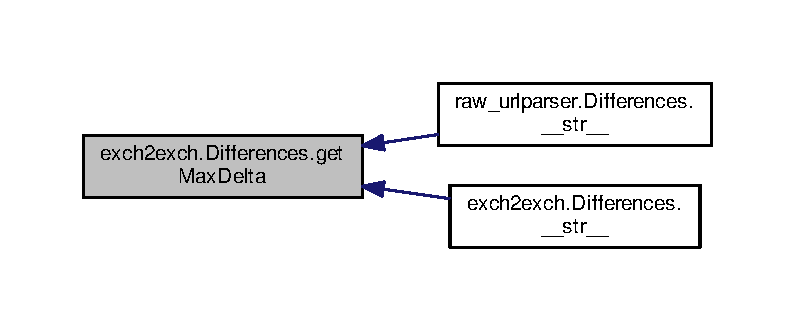
\includegraphics[width=350pt]{classexch2exch_1_1_differences_a3083b0bcc349937fb7ad708bc683e3d4_icgraph}
\end{center}
\end{figure}


\hypertarget{classexch2exch_1_1_differences_a83359c7999d33257746aa09f653e41fa}{\index{exch2exch\-::\-Differences@{exch2exch\-::\-Differences}!get\-Max\-Gain@{get\-Max\-Gain}}
\index{get\-Max\-Gain@{get\-Max\-Gain}!exch2exch::Differences@{exch2exch\-::\-Differences}}
\subsubsection[{get\-Max\-Gain}]{\setlength{\rightskip}{0pt plus 5cm}def exch2exch.\-Differences.\-get\-Max\-Gain (
\begin{DoxyParamCaption}
\item[{}]{self}
\end{DoxyParamCaption}
)}}\label{classexch2exch_1_1_differences_a83359c7999d33257746aa09f653e41fa}


Definition at line 121 of file exch2exch.\-py.



References exch2exch.\-Differences.\-gmax.



Referenced by exch2exch.\-Differences.\-\_\-\-\_\-str\-\_\-\-\_\-().


\begin{DoxyCode}
121 
122     \textcolor{keyword}{def }\hyperlink{classexch2exch_1_1_differences_a83359c7999d33257746aa09f653e41fa}{getMaxGain} (self): 
123         \textcolor{keywordflow}{return} self.\hyperlink{classexch2exch_1_1_differences_a569f2a6fa0e33ad725c3c3ada259ddcc}{gmax}
        
\end{DoxyCode}


Here is the caller graph for this function\-:
\nopagebreak
\begin{figure}[H]
\begin{center}
\leavevmode
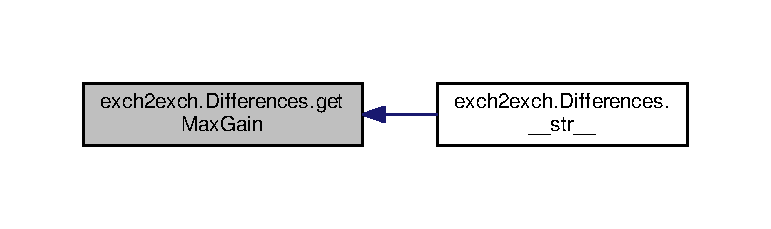
\includegraphics[width=350pt]{classexch2exch_1_1_differences_a83359c7999d33257746aa09f653e41fa_icgraph}
\end{center}
\end{figure}


\hypertarget{classexch2exch_1_1_differences_ae6156c3361371d1688de9b334ef7dc8d}{\index{exch2exch\-::\-Differences@{exch2exch\-::\-Differences}!get\-Min\-Delta@{get\-Min\-Delta}}
\index{get\-Min\-Delta@{get\-Min\-Delta}!exch2exch::Differences@{exch2exch\-::\-Differences}}
\subsubsection[{get\-Min\-Delta}]{\setlength{\rightskip}{0pt plus 5cm}def exch2exch.\-Differences.\-get\-Min\-Delta (
\begin{DoxyParamCaption}
\item[{}]{self}
\end{DoxyParamCaption}
)}}\label{classexch2exch_1_1_differences_ae6156c3361371d1688de9b334ef7dc8d}


Definition at line 112 of file exch2exch.\-py.



References exch2exch.\-Differences.\-dmin.



Referenced by raw\-\_\-urlparser.\-Differences.\-\_\-\-\_\-str\-\_\-\-\_\-(), and exch2exch.\-Differences.\-\_\-\-\_\-str\-\_\-\-\_\-().


\begin{DoxyCode}
112 
113     \textcolor{keyword}{def }\hyperlink{classexch2exch_1_1_differences_ae6156c3361371d1688de9b334ef7dc8d}{getMinDelta} (self):
114         \textcolor{keywordflow}{return} self.\hyperlink{classexch2exch_1_1_differences_a7825bfca16b5775aa770c8810412b215}{dmin}
        
\end{DoxyCode}


Here is the caller graph for this function\-:
\nopagebreak
\begin{figure}[H]
\begin{center}
\leavevmode
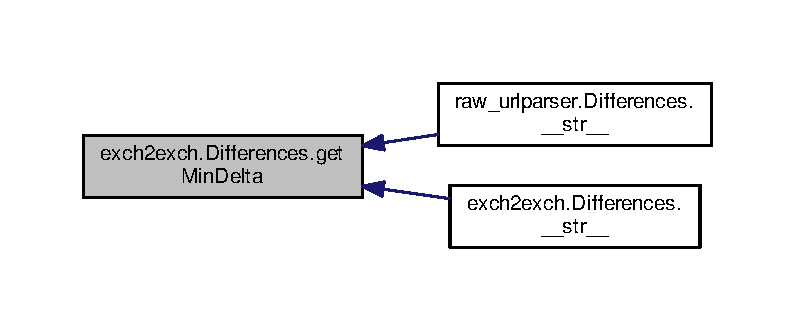
\includegraphics[width=350pt]{classexch2exch_1_1_differences_ae6156c3361371d1688de9b334ef7dc8d_icgraph}
\end{center}
\end{figure}


\hypertarget{classexch2exch_1_1_differences_a3c7fc587dedfda0e303260f244021017}{\index{exch2exch\-::\-Differences@{exch2exch\-::\-Differences}!get\-Min\-Gain@{get\-Min\-Gain}}
\index{get\-Min\-Gain@{get\-Min\-Gain}!exch2exch::Differences@{exch2exch\-::\-Differences}}
\subsubsection[{get\-Min\-Gain}]{\setlength{\rightskip}{0pt plus 5cm}def exch2exch.\-Differences.\-get\-Min\-Gain (
\begin{DoxyParamCaption}
\item[{}]{self}
\end{DoxyParamCaption}
)}}\label{classexch2exch_1_1_differences_a3c7fc587dedfda0e303260f244021017}


Definition at line 118 of file exch2exch.\-py.



References exch2exch.\-Differences.\-gmin.



Referenced by exch2exch.\-Differences.\-\_\-\-\_\-str\-\_\-\-\_\-().


\begin{DoxyCode}
118 
119     \textcolor{keyword}{def }\hyperlink{classexch2exch_1_1_differences_a3c7fc587dedfda0e303260f244021017}{getMinGain} (self):
120         \textcolor{keywordflow}{return} self.\hyperlink{classexch2exch_1_1_differences_a33c9add531b5b46c49ae322657343382}{gmin}
        
\end{DoxyCode}


Here is the caller graph for this function\-:
\nopagebreak
\begin{figure}[H]
\begin{center}
\leavevmode
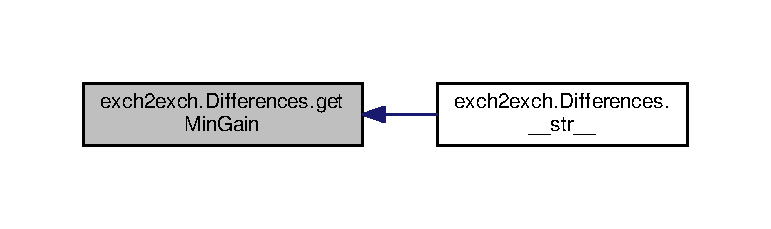
\includegraphics[width=350pt]{classexch2exch_1_1_differences_a3c7fc587dedfda0e303260f244021017_icgraph}
\end{center}
\end{figure}




\subsection{Member Data Documentation}
\hypertarget{classexch2exch_1_1_differences_a261a74cc25d77b2608898fa5611f9f0b}{\index{exch2exch\-::\-Differences@{exch2exch\-::\-Differences}!dmax@{dmax}}
\index{dmax@{dmax}!exch2exch::Differences@{exch2exch\-::\-Differences}}
\subsubsection[{dmax}]{\setlength{\rightskip}{0pt plus 5cm}exch2exch.\-Differences.\-dmax}}\label{classexch2exch_1_1_differences_a261a74cc25d77b2608898fa5611f9f0b}


Definition at line 107 of file exch2exch.\-py.



Referenced by raw\-\_\-urlparser.\-Differences.\-get\-Max\-Delta(), and exch2exch.\-Differences.\-get\-Max\-Delta().

\hypertarget{classexch2exch_1_1_differences_a7825bfca16b5775aa770c8810412b215}{\index{exch2exch\-::\-Differences@{exch2exch\-::\-Differences}!dmin@{dmin}}
\index{dmin@{dmin}!exch2exch::Differences@{exch2exch\-::\-Differences}}
\subsubsection[{dmin}]{\setlength{\rightskip}{0pt plus 5cm}exch2exch.\-Differences.\-dmin}}\label{classexch2exch_1_1_differences_a7825bfca16b5775aa770c8810412b215}


Definition at line 106 of file exch2exch.\-py.



Referenced by raw\-\_\-urlparser.\-Differences.\-get\-Min\-Delta(), and exch2exch.\-Differences.\-get\-Min\-Delta().

\hypertarget{classexch2exch_1_1_differences_a569f2a6fa0e33ad725c3c3ada259ddcc}{\index{exch2exch\-::\-Differences@{exch2exch\-::\-Differences}!gmax@{gmax}}
\index{gmax@{gmax}!exch2exch::Differences@{exch2exch\-::\-Differences}}
\subsubsection[{gmax}]{\setlength{\rightskip}{0pt plus 5cm}exch2exch.\-Differences.\-gmax}}\label{classexch2exch_1_1_differences_a569f2a6fa0e33ad725c3c3ada259ddcc}


Definition at line 110 of file exch2exch.\-py.



Referenced by exch2exch.\-Differences.\-get\-Max\-Gain().

\hypertarget{classexch2exch_1_1_differences_a33c9add531b5b46c49ae322657343382}{\index{exch2exch\-::\-Differences@{exch2exch\-::\-Differences}!gmin@{gmin}}
\index{gmin@{gmin}!exch2exch::Differences@{exch2exch\-::\-Differences}}
\subsubsection[{gmin}]{\setlength{\rightskip}{0pt plus 5cm}exch2exch.\-Differences.\-gmin}}\label{classexch2exch_1_1_differences_a33c9add531b5b46c49ae322657343382}


Definition at line 109 of file exch2exch.\-py.



Referenced by exch2exch.\-Differences.\-get\-Min\-Gain().

\hypertarget{classexch2exch_1_1_differences_a81c81e9c15b5ea8a5d39bb99d85250e1}{\index{exch2exch\-::\-Differences@{exch2exch\-::\-Differences}!mb@{mb}}
\index{mb@{mb}!exch2exch::Differences@{exch2exch\-::\-Differences}}
\subsubsection[{mb}]{\setlength{\rightskip}{0pt plus 5cm}exch2exch.\-Differences.\-mb}}\label{classexch2exch_1_1_differences_a81c81e9c15b5ea8a5d39bb99d85250e1}


Definition at line 103 of file exch2exch.\-py.

\hypertarget{classexch2exch_1_1_differences_a6de3ee563584c83a97ba815db8ec7831}{\index{exch2exch\-::\-Differences@{exch2exch\-::\-Differences}!ok@{ok}}
\index{ok@{ok}!exch2exch::Differences@{exch2exch\-::\-Differences}}
\subsubsection[{ok}]{\setlength{\rightskip}{0pt plus 5cm}exch2exch.\-Differences.\-ok}}\label{classexch2exch_1_1_differences_a6de3ee563584c83a97ba815db8ec7831}


Definition at line 104 of file exch2exch.\-py.

\hypertarget{classexch2exch_1_1_differences_a64aec2fc7f20028f0bd834908cbea116}{\index{exch2exch\-::\-Differences@{exch2exch\-::\-Differences}!rates@{rates}}
\index{rates@{rates}!exch2exch::Differences@{exch2exch\-::\-Differences}}
\subsubsection[{rates}]{\setlength{\rightskip}{0pt plus 5cm}exch2exch.\-Differences.\-rates}}\label{classexch2exch_1_1_differences_a64aec2fc7f20028f0bd834908cbea116}


Definition at line 102 of file exch2exch.\-py.



The documentation for this class was generated from the following file\-:\begin{DoxyCompactItemize}
\item 
/home/hilton/github/exch2exh/\hyperlink{exch2exch_8py}{exch2exch.\-py}\end{DoxyCompactItemize}

\hypertarget{classraw__urlparser_1_1_differences}{}\section{raw\+\_\+urlparser.\+Differences Class Reference}
\label{classraw__urlparser_1_1_differences}\index{raw\+\_\+urlparser.\+Differences@{raw\+\_\+urlparser.\+Differences}}


Collaboration diagram for raw\+\_\+urlparser.\+Differences\+:\nopagebreak
\begin{figure}[H]
\begin{center}
\leavevmode
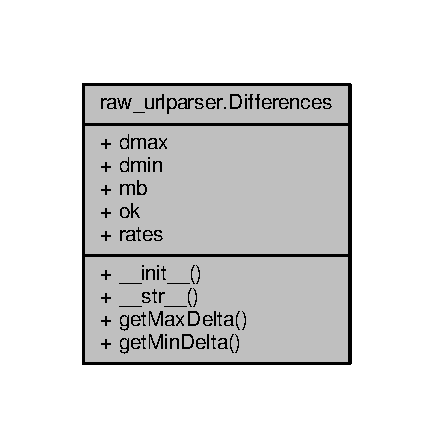
\includegraphics[width=208pt]{classraw__urlparser_1_1_differences__coll__graph}
\end{center}
\end{figure}
\subsection*{Public Member Functions}
\begin{DoxyCompactItemize}
\item 
def \hyperlink{classraw__urlparser_1_1_differences_ab96f235ba2697e17fea2e3dc83ab2ca0}{\+\_\+\+\_\+init\+\_\+\+\_\+} (self, \hyperlink{classraw__urlparser_1_1_differences_ad4e7eadb659a1cdcba90793cc52af174}{rates}, \hyperlink{classraw__urlparser_1_1_differences_ab4c3073b8c569b7791ab3b8e21e9b364}{mb}, \hyperlink{classraw__urlparser_1_1_differences_a46fe97bedb977585a0b27d7408ace118}{ok})
\item 
def \hyperlink{classraw__urlparser_1_1_differences_ae30a248dbbe9fde42b0bcbd81160f070}{\+\_\+\+\_\+str\+\_\+\+\_\+} (self)
\item 
def \hyperlink{classraw__urlparser_1_1_differences_acfa09d743c08cc813a5bc435aa6875da}{get\+Max\+Delta} (self)
\item 
def \hyperlink{classraw__urlparser_1_1_differences_af19faaea85ca8ac0d327c8443ddd99ef}{get\+Min\+Delta} (self)
\end{DoxyCompactItemize}
\subsection*{Public Attributes}
\begin{DoxyCompactItemize}
\item 
\hyperlink{classraw__urlparser_1_1_differences_ad2b06158b655136bc7743dc6ac8d1e2a}{dmax}
\item 
\hyperlink{classraw__urlparser_1_1_differences_af8457a8e542de086595e7fbbffdf713c}{dmin}
\item 
\hyperlink{classraw__urlparser_1_1_differences_ab4c3073b8c569b7791ab3b8e21e9b364}{mb}
\item 
\hyperlink{classraw__urlparser_1_1_differences_a46fe97bedb977585a0b27d7408ace118}{ok}
\item 
\hyperlink{classraw__urlparser_1_1_differences_ad4e7eadb659a1cdcba90793cc52af174}{rates}
\end{DoxyCompactItemize}


\subsection{Detailed Description}


Definition at line \hyperlink{raw__urlparser_8py_source_l00084}{84} of file \hyperlink{raw__urlparser_8py_source}{raw\+\_\+urlparser.\+py}.



\subsection{Constructor \& Destructor Documentation}
\index{raw\+\_\+urlparser\+::\+Differences@{raw\+\_\+urlparser\+::\+Differences}!\+\_\+\+\_\+init\+\_\+\+\_\+@{\+\_\+\+\_\+init\+\_\+\+\_\+}}
\index{\+\_\+\+\_\+init\+\_\+\+\_\+@{\+\_\+\+\_\+init\+\_\+\+\_\+}!raw\+\_\+urlparser\+::\+Differences@{raw\+\_\+urlparser\+::\+Differences}}
\subsubsection[{\texorpdfstring{\+\_\+\+\_\+init\+\_\+\+\_\+(self, rates, mb, ok)}{__init__(self, rates, mb, ok)}}]{\setlength{\rightskip}{0pt plus 5cm}def raw\+\_\+urlparser.\+Differences.\+\_\+\+\_\+init\+\_\+\+\_\+ (
\begin{DoxyParamCaption}
\item[{}]{self, }
\item[{}]{rates, }
\item[{}]{mb, }
\item[{}]{ok}
\end{DoxyParamCaption}
)}\hypertarget{classraw__urlparser_1_1_differences_ab96f235ba2697e17fea2e3dc83ab2ca0}{}\label{classraw__urlparser_1_1_differences_ab96f235ba2697e17fea2e3dc83ab2ca0}


Definition at line \hyperlink{raw__urlparser_8py_source_l00085}{85} of file \hyperlink{raw__urlparser_8py_source}{raw\+\_\+urlparser.\+py}.


\begin{DoxyCode}
\hypertarget{classraw__urlparser_1_1_differences.tex_l00085}{}\hyperlink{classraw__urlparser_1_1_differences_ab96f235ba2697e17fea2e3dc83ab2ca0}{00085}     \textcolor{keyword}{def }\hyperlink{classraw__urlparser_1_1_differences_ab96f235ba2697e17fea2e3dc83ab2ca0}{\_\_init\_\_} (self, rates, mb, ok):
\hypertarget{classraw__urlparser_1_1_differences.tex_l00086}{}\hyperlink{classraw__urlparser_1_1_differences_ad4e7eadb659a1cdcba90793cc52af174}{00086}         self.\hyperlink{classraw__urlparser_1_1_differences_ad4e7eadb659a1cdcba90793cc52af174}{rates} = rates
\hypertarget{classraw__urlparser_1_1_differences.tex_l00087}{}\hyperlink{classraw__urlparser_1_1_differences_ab4c3073b8c569b7791ab3b8e21e9b364}{00087}         self.\hyperlink{classraw__urlparser_1_1_differences_ab4c3073b8c569b7791ab3b8e21e9b364}{mb} = mb
\hypertarget{classraw__urlparser_1_1_differences.tex_l00088}{}\hyperlink{classraw__urlparser_1_1_differences_a46fe97bedb977585a0b27d7408ace118}{00088}         self.\hyperlink{classraw__urlparser_1_1_differences_a46fe97bedb977585a0b27d7408ace118}{ok} = ok
00089         
\hypertarget{classraw__urlparser_1_1_differences.tex_l00090}{}\hyperlink{classraw__urlparser_1_1_differences_af8457a8e542de086595e7fbbffdf713c}{00090}         self.\hyperlink{classraw__urlparser_1_1_differences_af8457a8e542de086595e7fbbffdf713c}{dmin} = mb.getSell () - ok.getSell ()
00091         
\hypertarget{classraw__urlparser_1_1_differences.tex_l00092}{}\hyperlink{classraw__urlparser_1_1_differences_ad2b06158b655136bc7743dc6ac8d1e2a}{00092}         self.\hyperlink{classraw__urlparser_1_1_differences_ad2b06158b655136bc7743dc6ac8d1e2a}{dmax} = mb.getBuy () - ok.getSell ()
00093         
\end{DoxyCode}


\subsection{Member Function Documentation}
\index{raw\+\_\+urlparser\+::\+Differences@{raw\+\_\+urlparser\+::\+Differences}!\+\_\+\+\_\+str\+\_\+\+\_\+@{\+\_\+\+\_\+str\+\_\+\+\_\+}}
\index{\+\_\+\+\_\+str\+\_\+\+\_\+@{\+\_\+\+\_\+str\+\_\+\+\_\+}!raw\+\_\+urlparser\+::\+Differences@{raw\+\_\+urlparser\+::\+Differences}}
\subsubsection[{\texorpdfstring{\+\_\+\+\_\+str\+\_\+\+\_\+(self)}{__str__(self)}}]{\setlength{\rightskip}{0pt plus 5cm}def raw\+\_\+urlparser.\+Differences.\+\_\+\+\_\+str\+\_\+\+\_\+ (
\begin{DoxyParamCaption}
\item[{}]{self}
\end{DoxyParamCaption}
)}\hypertarget{classraw__urlparser_1_1_differences_ae30a248dbbe9fde42b0bcbd81160f070}{}\label{classraw__urlparser_1_1_differences_ae30a248dbbe9fde42b0bcbd81160f070}


Definition at line \hyperlink{raw__urlparser_8py_source_l00100}{100} of file \hyperlink{raw__urlparser_8py_source}{raw\+\_\+urlparser.\+py}.



References \hyperlink{raw__urlparser_8py_source_l00097}{raw\+\_\+urlparser.\+Differences.\+get\+Max\+Delta()}, \hyperlink{exch2exch_8py_source_l00130}{exch2exch.\+Differences.\+get\+Max\+Delta()}, \hyperlink{raw__urlparser_8py_source_l00094}{raw\+\_\+urlparser.\+Differences.\+get\+Min\+Delta()}, and \hyperlink{exch2exch_8py_source_l00127}{exch2exch.\+Differences.\+get\+Min\+Delta()}.


\begin{DoxyCode}
\hypertarget{classraw__urlparser_1_1_differences.tex_l00100}{}\hyperlink{classraw__urlparser_1_1_differences_ae30a248dbbe9fde42b0bcbd81160f070}{00100}     \textcolor{keyword}{def }\hyperlink{classraw__urlparser_1_1_differences_ae30a248dbbe9fde42b0bcbd81160f070}{\_\_str\_\_} (self):
00101         result = \textcolor{stringliteral}{""}
00102         
00103         oname = self.ok.getExchangeName ()
00104         mname = self.ok.getExchangeName ()
00105         sname = self.rates.getServiceName ()
00106         
00107         fmt = \textcolor{stringliteral}{"Calculation between \{0\} and \{1\} rates, with conversion from \{1\}"}
00108         result = fmt.format (oname, mname, sname)
00109         fmt = \textcolor{stringliteral}{"\(\backslash\)nIntervals: minimum \{0:.4f\}, maximum \{1:.4f\}"}
00110         result += fmt.format (self.\hyperlink{classraw__urlparser_1_1_differences_af19faaea85ca8ac0d327c8443ddd99ef}{getMinDelta} (), self.\hyperlink{classraw__urlparser_1_1_differences_acfa09d743c08cc813a5bc435aa6875da}{getMaxDelta} ())
00111         \textcolor{keywordflow}{return} result
00112 
00113 \textcolor{comment}{#        }
00114 \textcolor{comment}{# }
00115 \textcolor{comment}{# Google section }
00116 \textcolor{comment}{#}
00117 
\end{DoxyCode}


Here is the call graph for this function\+:\nopagebreak
\begin{figure}[H]
\begin{center}
\leavevmode
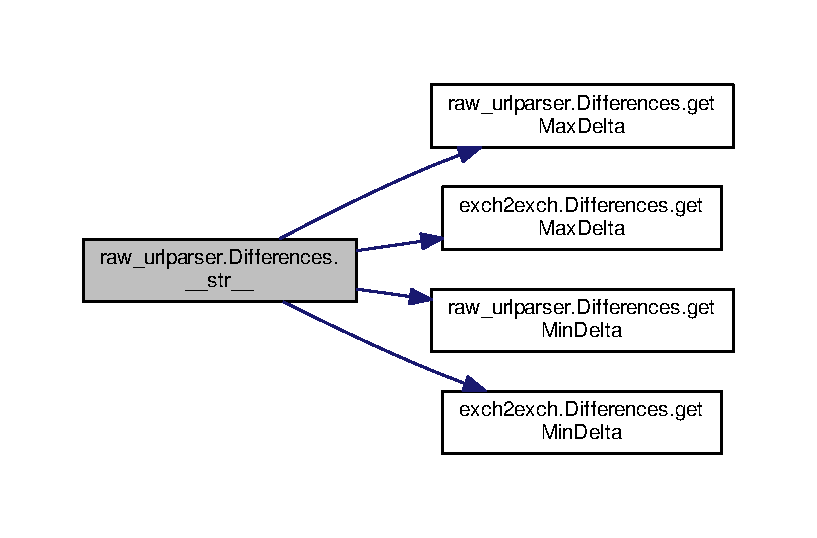
\includegraphics[width=350pt]{classraw__urlparser_1_1_differences_ae30a248dbbe9fde42b0bcbd81160f070_cgraph}
\end{center}
\end{figure}


\index{raw\+\_\+urlparser\+::\+Differences@{raw\+\_\+urlparser\+::\+Differences}!get\+Max\+Delta@{get\+Max\+Delta}}
\index{get\+Max\+Delta@{get\+Max\+Delta}!raw\+\_\+urlparser\+::\+Differences@{raw\+\_\+urlparser\+::\+Differences}}
\subsubsection[{\texorpdfstring{get\+Max\+Delta(self)}{getMaxDelta(self)}}]{\setlength{\rightskip}{0pt plus 5cm}def raw\+\_\+urlparser.\+Differences.\+get\+Max\+Delta (
\begin{DoxyParamCaption}
\item[{}]{self}
\end{DoxyParamCaption}
)}\hypertarget{classraw__urlparser_1_1_differences_acfa09d743c08cc813a5bc435aa6875da}{}\label{classraw__urlparser_1_1_differences_acfa09d743c08cc813a5bc435aa6875da}


Definition at line \hyperlink{raw__urlparser_8py_source_l00097}{97} of file \hyperlink{raw__urlparser_8py_source}{raw\+\_\+urlparser.\+py}.



References \hyperlink{raw__urlparser_8py_source_l00092}{raw\+\_\+urlparser.\+Differences.\+dmax}, \hyperlink{exch2exch_8py_source_l00115}{exch2exch.\+Differences.\+dmax}, and \hyperlink{exchange_8py_source_l00259}{exchange.\+Diff\+Tracker.\+dmax}.



Referenced by \hyperlink{raw__urlparser_8py_source_l00100}{raw\+\_\+urlparser.\+Differences.\+\_\+\+\_\+str\+\_\+\+\_\+()}.


\begin{DoxyCode}
\hypertarget{classraw__urlparser_1_1_differences.tex_l00097}{}\hyperlink{classraw__urlparser_1_1_differences_acfa09d743c08cc813a5bc435aa6875da}{00097}     \textcolor{keyword}{def }\hyperlink{classraw__urlparser_1_1_differences_acfa09d743c08cc813a5bc435aa6875da}{getMaxDelta} (self):
00098         \textcolor{keywordflow}{return} self.\hyperlink{classraw__urlparser_1_1_differences_ad2b06158b655136bc7743dc6ac8d1e2a}{dmax}
00099         
\end{DoxyCode}


Here is the caller graph for this function\+:\nopagebreak
\begin{figure}[H]
\begin{center}
\leavevmode
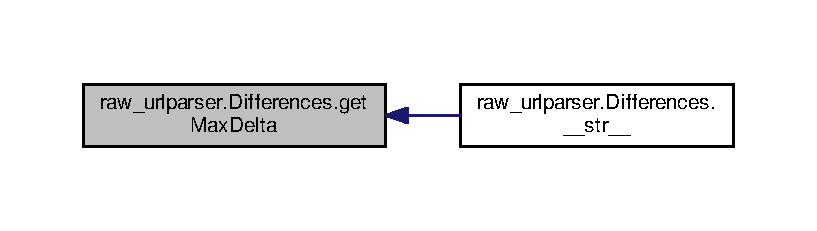
\includegraphics[width=350pt]{classraw__urlparser_1_1_differences_acfa09d743c08cc813a5bc435aa6875da_icgraph}
\end{center}
\end{figure}


\index{raw\+\_\+urlparser\+::\+Differences@{raw\+\_\+urlparser\+::\+Differences}!get\+Min\+Delta@{get\+Min\+Delta}}
\index{get\+Min\+Delta@{get\+Min\+Delta}!raw\+\_\+urlparser\+::\+Differences@{raw\+\_\+urlparser\+::\+Differences}}
\subsubsection[{\texorpdfstring{get\+Min\+Delta(self)}{getMinDelta(self)}}]{\setlength{\rightskip}{0pt plus 5cm}def raw\+\_\+urlparser.\+Differences.\+get\+Min\+Delta (
\begin{DoxyParamCaption}
\item[{}]{self}
\end{DoxyParamCaption}
)}\hypertarget{classraw__urlparser_1_1_differences_af19faaea85ca8ac0d327c8443ddd99ef}{}\label{classraw__urlparser_1_1_differences_af19faaea85ca8ac0d327c8443ddd99ef}


Definition at line \hyperlink{raw__urlparser_8py_source_l00094}{94} of file \hyperlink{raw__urlparser_8py_source}{raw\+\_\+urlparser.\+py}.



References \hyperlink{raw__urlparser_8py_source_l00090}{raw\+\_\+urlparser.\+Differences.\+dmin}, \hyperlink{exch2exch_8py_source_l00116}{exch2exch.\+Differences.\+dmin}, and \hyperlink{exchange_8py_source_l00260}{exchange.\+Diff\+Tracker.\+dmin}.



Referenced by \hyperlink{raw__urlparser_8py_source_l00100}{raw\+\_\+urlparser.\+Differences.\+\_\+\+\_\+str\+\_\+\+\_\+()}.


\begin{DoxyCode}
\hypertarget{classraw__urlparser_1_1_differences.tex_l00094}{}\hyperlink{classraw__urlparser_1_1_differences_af19faaea85ca8ac0d327c8443ddd99ef}{00094}     \textcolor{keyword}{def }\hyperlink{classraw__urlparser_1_1_differences_af19faaea85ca8ac0d327c8443ddd99ef}{getMinDelta} (self):
00095         \textcolor{keywordflow}{return} self.\hyperlink{classraw__urlparser_1_1_differences_af8457a8e542de086595e7fbbffdf713c}{dmin}
00096         
\end{DoxyCode}


Here is the caller graph for this function\+:\nopagebreak
\begin{figure}[H]
\begin{center}
\leavevmode
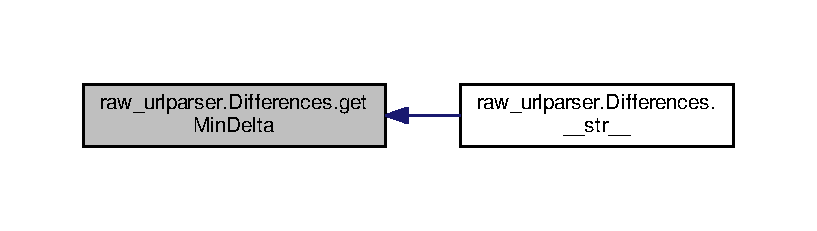
\includegraphics[width=350pt]{classraw__urlparser_1_1_differences_af19faaea85ca8ac0d327c8443ddd99ef_icgraph}
\end{center}
\end{figure}




\subsection{Member Data Documentation}
\index{raw\+\_\+urlparser\+::\+Differences@{raw\+\_\+urlparser\+::\+Differences}!dmax@{dmax}}
\index{dmax@{dmax}!raw\+\_\+urlparser\+::\+Differences@{raw\+\_\+urlparser\+::\+Differences}}
\subsubsection[{\texorpdfstring{dmax}{dmax}}]{\setlength{\rightskip}{0pt plus 5cm}raw\+\_\+urlparser.\+Differences.\+dmax}\hypertarget{classraw__urlparser_1_1_differences_ad2b06158b655136bc7743dc6ac8d1e2a}{}\label{classraw__urlparser_1_1_differences_ad2b06158b655136bc7743dc6ac8d1e2a}


Definition at line \hyperlink{raw__urlparser_8py_source_l00092}{92} of file \hyperlink{raw__urlparser_8py_source}{raw\+\_\+urlparser.\+py}.



Referenced by \hyperlink{raw__urlparser_8py_source_l00097}{raw\+\_\+urlparser.\+Differences.\+get\+Max\+Delta()}.

\index{raw\+\_\+urlparser\+::\+Differences@{raw\+\_\+urlparser\+::\+Differences}!dmin@{dmin}}
\index{dmin@{dmin}!raw\+\_\+urlparser\+::\+Differences@{raw\+\_\+urlparser\+::\+Differences}}
\subsubsection[{\texorpdfstring{dmin}{dmin}}]{\setlength{\rightskip}{0pt plus 5cm}raw\+\_\+urlparser.\+Differences.\+dmin}\hypertarget{classraw__urlparser_1_1_differences_af8457a8e542de086595e7fbbffdf713c}{}\label{classraw__urlparser_1_1_differences_af8457a8e542de086595e7fbbffdf713c}


Definition at line \hyperlink{raw__urlparser_8py_source_l00090}{90} of file \hyperlink{raw__urlparser_8py_source}{raw\+\_\+urlparser.\+py}.



Referenced by \hyperlink{raw__urlparser_8py_source_l00094}{raw\+\_\+urlparser.\+Differences.\+get\+Min\+Delta()}.

\index{raw\+\_\+urlparser\+::\+Differences@{raw\+\_\+urlparser\+::\+Differences}!mb@{mb}}
\index{mb@{mb}!raw\+\_\+urlparser\+::\+Differences@{raw\+\_\+urlparser\+::\+Differences}}
\subsubsection[{\texorpdfstring{mb}{mb}}]{\setlength{\rightskip}{0pt plus 5cm}raw\+\_\+urlparser.\+Differences.\+mb}\hypertarget{classraw__urlparser_1_1_differences_ab4c3073b8c569b7791ab3b8e21e9b364}{}\label{classraw__urlparser_1_1_differences_ab4c3073b8c569b7791ab3b8e21e9b364}


Definition at line \hyperlink{raw__urlparser_8py_source_l00087}{87} of file \hyperlink{raw__urlparser_8py_source}{raw\+\_\+urlparser.\+py}.

\index{raw\+\_\+urlparser\+::\+Differences@{raw\+\_\+urlparser\+::\+Differences}!ok@{ok}}
\index{ok@{ok}!raw\+\_\+urlparser\+::\+Differences@{raw\+\_\+urlparser\+::\+Differences}}
\subsubsection[{\texorpdfstring{ok}{ok}}]{\setlength{\rightskip}{0pt plus 5cm}raw\+\_\+urlparser.\+Differences.\+ok}\hypertarget{classraw__urlparser_1_1_differences_a46fe97bedb977585a0b27d7408ace118}{}\label{classraw__urlparser_1_1_differences_a46fe97bedb977585a0b27d7408ace118}


Definition at line \hyperlink{raw__urlparser_8py_source_l00088}{88} of file \hyperlink{raw__urlparser_8py_source}{raw\+\_\+urlparser.\+py}.

\index{raw\+\_\+urlparser\+::\+Differences@{raw\+\_\+urlparser\+::\+Differences}!rates@{rates}}
\index{rates@{rates}!raw\+\_\+urlparser\+::\+Differences@{raw\+\_\+urlparser\+::\+Differences}}
\subsubsection[{\texorpdfstring{rates}{rates}}]{\setlength{\rightskip}{0pt plus 5cm}raw\+\_\+urlparser.\+Differences.\+rates}\hypertarget{classraw__urlparser_1_1_differences_ad4e7eadb659a1cdcba90793cc52af174}{}\label{classraw__urlparser_1_1_differences_ad4e7eadb659a1cdcba90793cc52af174}


Definition at line \hyperlink{raw__urlparser_8py_source_l00086}{86} of file \hyperlink{raw__urlparser_8py_source}{raw\+\_\+urlparser.\+py}.



The documentation for this class was generated from the following file\+:\begin{DoxyCompactItemize}
\item 
/home/hilton/github/exch2exh/\hyperlink{raw__urlparser_8py}{raw\+\_\+urlparser.\+py}\end{DoxyCompactItemize}

\hypertarget{classgen__factory_1_1_dummy}{}\section{gen\+\_\+factory.\+Dummy Class Reference}
\label{classgen__factory_1_1_dummy}\index{gen\+\_\+factory.\+Dummy@{gen\+\_\+factory.\+Dummy}}


Inheritance diagram for gen\+\_\+factory.\+Dummy\+:\nopagebreak
\begin{figure}[H]
\begin{center}
\leavevmode
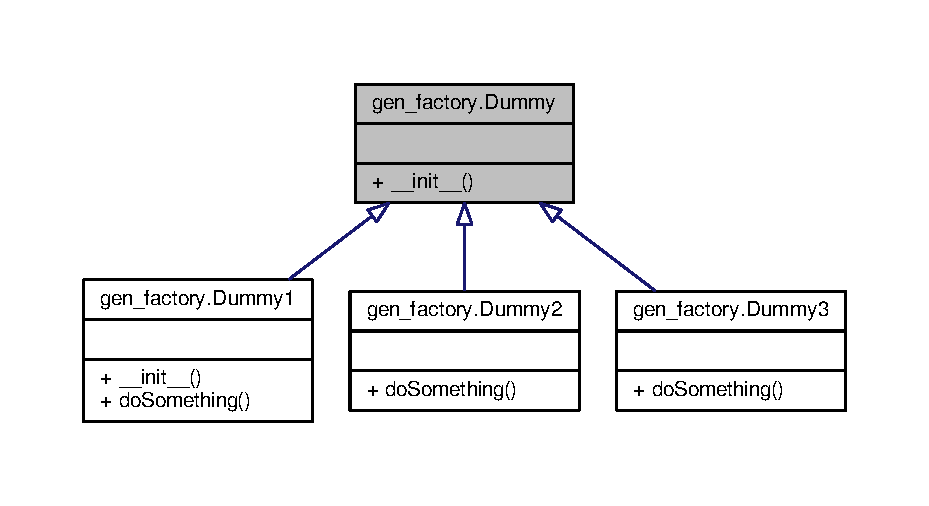
\includegraphics[width=350pt]{classgen__factory_1_1_dummy__inherit__graph}
\end{center}
\end{figure}


Collaboration diagram for gen\+\_\+factory.\+Dummy\+:\nopagebreak
\begin{figure}[H]
\begin{center}
\leavevmode
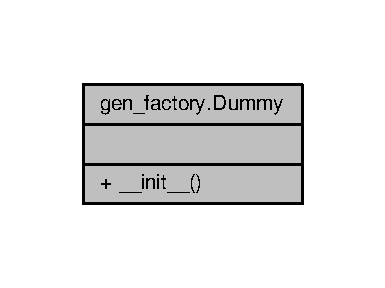
\includegraphics[width=185pt]{classgen__factory_1_1_dummy__coll__graph}
\end{center}
\end{figure}
\subsection*{Public Member Functions}
\begin{DoxyCompactItemize}
\item 
def \hyperlink{classgen__factory_1_1_dummy_aed8c66d829aedd98a5b1bed80725ffab}{\+\_\+\+\_\+init\+\_\+\+\_\+} (self)
\end{DoxyCompactItemize}


\subsection{Detailed Description}


Definition at line \hyperlink{gen__factory_8py_source_l00009}{9} of file \hyperlink{gen__factory_8py_source}{gen\+\_\+factory.\+py}.



\subsection{Constructor \& Destructor Documentation}
\index{gen\+\_\+factory\+::\+Dummy@{gen\+\_\+factory\+::\+Dummy}!\+\_\+\+\_\+init\+\_\+\+\_\+@{\+\_\+\+\_\+init\+\_\+\+\_\+}}
\index{\+\_\+\+\_\+init\+\_\+\+\_\+@{\+\_\+\+\_\+init\+\_\+\+\_\+}!gen\+\_\+factory\+::\+Dummy@{gen\+\_\+factory\+::\+Dummy}}
\subsubsection[{\texorpdfstring{\+\_\+\+\_\+init\+\_\+\+\_\+(self)}{__init__(self)}}]{\setlength{\rightskip}{0pt plus 5cm}def gen\+\_\+factory.\+Dummy.\+\_\+\+\_\+init\+\_\+\+\_\+ (
\begin{DoxyParamCaption}
\item[{}]{self}
\end{DoxyParamCaption}
)}\hypertarget{classgen__factory_1_1_dummy_aed8c66d829aedd98a5b1bed80725ffab}{}\label{classgen__factory_1_1_dummy_aed8c66d829aedd98a5b1bed80725ffab}


Definition at line \hyperlink{gen__factory_8py_source_l00010}{10} of file \hyperlink{gen__factory_8py_source}{gen\+\_\+factory.\+py}.


\begin{DoxyCode}
\hypertarget{classgen__factory_1_1_dummy.tex_l00010}{}\hyperlink{classgen__factory_1_1_dummy_aed8c66d829aedd98a5b1bed80725ffab}{00010}     \textcolor{keyword}{def }\hyperlink{classgen__factory_1_1_dummy_aed8c66d829aedd98a5b1bed80725ffab}{\_\_init\_\_} (self):
00011         \textcolor{keywordflow}{print} (\textcolor{stringliteral}{"\{0\}.\_\_init\_\_() "}.format (self.\_\_class\_\_.\_\_name\_\_))
00012 
\end{DoxyCode}


The documentation for this class was generated from the following file\+:\begin{DoxyCompactItemize}
\item 
/home/hilton/github/exch2exh/\hyperlink{gen__factory_8py}{gen\+\_\+factory.\+py}\end{DoxyCompactItemize}

\hypertarget{classgen__factory_1_1_dummy1}{}\section{gen\+\_\+factory.\+Dummy1 Class Reference}
\label{classgen__factory_1_1_dummy1}\index{gen\+\_\+factory.\+Dummy1@{gen\+\_\+factory.\+Dummy1}}


Inheritance diagram for gen\+\_\+factory.\+Dummy1\+:
\nopagebreak
\begin{figure}[H]
\begin{center}
\leavevmode
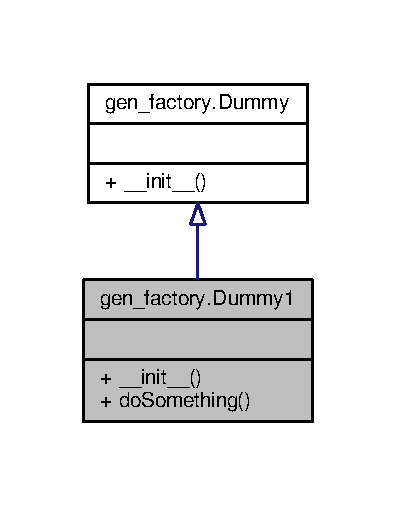
\includegraphics[width=190pt]{classgen__factory_1_1_dummy1__inherit__graph}
\end{center}
\end{figure}


Collaboration diagram for gen\+\_\+factory.\+Dummy1\+:
\nopagebreak
\begin{figure}[H]
\begin{center}
\leavevmode
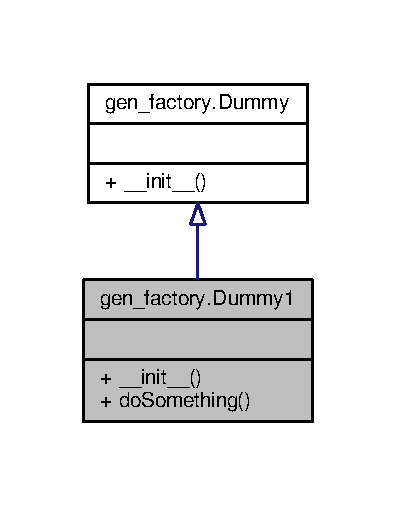
\includegraphics[width=190pt]{classgen__factory_1_1_dummy1__coll__graph}
\end{center}
\end{figure}
\subsection*{Public Member Functions}
\begin{DoxyCompactItemize}
\item 
def \hyperlink{classgen__factory_1_1_dummy1_a9bb75256a466ee77a0ae2cafb339fe62}{\+\_\+\+\_\+init\+\_\+\+\_\+} (self)
\item 
def \hyperlink{classgen__factory_1_1_dummy1_af8a40601dbd998624323da24581dfa1c}{do\+Something} (self)
\end{DoxyCompactItemize}


\subsection{Detailed Description}


Definition at line \hyperlink{gen__factory_8py_source_l00013}{13} of file \hyperlink{gen__factory_8py_source}{gen\+\_\+factory.\+py}.



\subsection{Constructor \& Destructor Documentation}
\mbox{\Hypertarget{classgen__factory_1_1_dummy1_a9bb75256a466ee77a0ae2cafb339fe62}\label{classgen__factory_1_1_dummy1_a9bb75256a466ee77a0ae2cafb339fe62}} 
\index{gen\+\_\+factory\+::\+Dummy1@{gen\+\_\+factory\+::\+Dummy1}!\+\_\+\+\_\+init\+\_\+\+\_\+@{\+\_\+\+\_\+init\+\_\+\+\_\+}}
\index{\+\_\+\+\_\+init\+\_\+\+\_\+@{\+\_\+\+\_\+init\+\_\+\+\_\+}!gen\+\_\+factory\+::\+Dummy1@{gen\+\_\+factory\+::\+Dummy1}}
\subsubsection{\texorpdfstring{\+\_\+\+\_\+init\+\_\+\+\_\+()}{\_\_init\_\_()}}
{\footnotesize\ttfamily def gen\+\_\+factory.\+Dummy1.\+\_\+\+\_\+init\+\_\+\+\_\+ (\begin{DoxyParamCaption}\item[{}]{self }\end{DoxyParamCaption})}



Definition at line \hyperlink{gen__factory_8py_source_l00014}{14} of file \hyperlink{gen__factory_8py_source}{gen\+\_\+factory.\+py}.


\begin{DoxyCode}
00014     \textcolor{keyword}{def }\hyperlink{namespacestart__time_a9c9bd378729a13c96a22c8b079ea172c}{\_\_init\_\_} (self):
00015         \textcolor{keywordflow}{print} (\textcolor{stringliteral}{"\{0\}.\_\_init\_\_() "}.format (self.\_\_class\_\_.\_\_name\_\_))
00016         
00017 \textcolor{comment}{#    def \_\_new\_\_ (self):}
00018 \textcolor{comment}{#        print ("Dummy1.\_\_new\_\_() ", self.\_\_class\_\_.\_\_name\_\_)}
00019 \textcolor{comment}{#        Dummy1.\_\_init\_\_ (self)}
00020         
\end{DoxyCode}


\subsection{Member Function Documentation}
\mbox{\Hypertarget{classgen__factory_1_1_dummy1_af8a40601dbd998624323da24581dfa1c}\label{classgen__factory_1_1_dummy1_af8a40601dbd998624323da24581dfa1c}} 
\index{gen\+\_\+factory\+::\+Dummy1@{gen\+\_\+factory\+::\+Dummy1}!do\+Something@{do\+Something}}
\index{do\+Something@{do\+Something}!gen\+\_\+factory\+::\+Dummy1@{gen\+\_\+factory\+::\+Dummy1}}
\subsubsection{\texorpdfstring{do\+Something()}{doSomething()}}
{\footnotesize\ttfamily def gen\+\_\+factory.\+Dummy1.\+do\+Something (\begin{DoxyParamCaption}\item[{}]{self }\end{DoxyParamCaption})}



Definition at line \hyperlink{gen__factory_8py_source_l00021}{21} of file \hyperlink{gen__factory_8py_source}{gen\+\_\+factory.\+py}.


\begin{DoxyCode}
00021     \textcolor{keyword}{def }doSomething (self):
00022         \textcolor{keywordflow}{print} (\textcolor{stringliteral}{"I'm an instance of class \{0\}"}. format (type (self).\_\_name\_\_))
00023 
\end{DoxyCode}


The documentation for this class was generated from the following file\+:\begin{DoxyCompactItemize}
\item 
/home/hilton/github/exch2exh/\hyperlink{gen__factory_8py}{gen\+\_\+factory.\+py}\end{DoxyCompactItemize}

\hypertarget{classgen__factory_1_1_dummy2}{}\section{gen\+\_\+factory.\+Dummy2 Class Reference}
\label{classgen__factory_1_1_dummy2}\index{gen\+\_\+factory.\+Dummy2@{gen\+\_\+factory.\+Dummy2}}


Inheritance diagram for gen\+\_\+factory.\+Dummy2\+:
\nopagebreak
\begin{figure}[H]
\begin{center}
\leavevmode
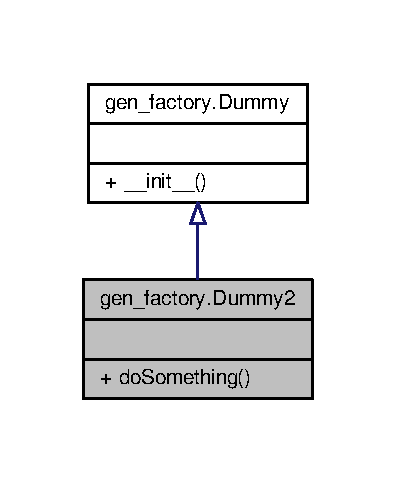
\includegraphics[width=190pt]{classgen__factory_1_1_dummy2__inherit__graph}
\end{center}
\end{figure}


Collaboration diagram for gen\+\_\+factory.\+Dummy2\+:
\nopagebreak
\begin{figure}[H]
\begin{center}
\leavevmode
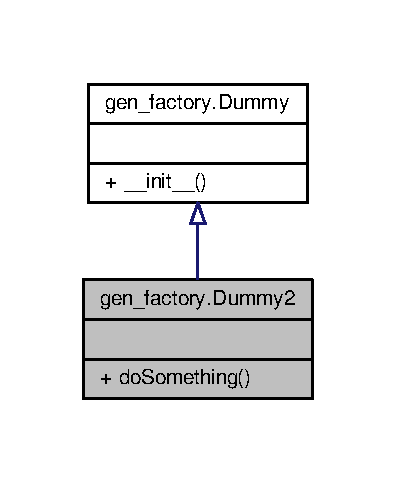
\includegraphics[width=190pt]{classgen__factory_1_1_dummy2__coll__graph}
\end{center}
\end{figure}
\subsection*{Public Member Functions}
\begin{DoxyCompactItemize}
\item 
def \hyperlink{classgen__factory_1_1_dummy2_a22fc655957f756c7967b655b83375c66}{do\+Something} (self)
\end{DoxyCompactItemize}


\subsection{Detailed Description}


Definition at line \hyperlink{gen__factory_8py_source_l00024}{24} of file \hyperlink{gen__factory_8py_source}{gen\+\_\+factory.\+py}.



\subsection{Member Function Documentation}
\mbox{\Hypertarget{classgen__factory_1_1_dummy2_a22fc655957f756c7967b655b83375c66}\label{classgen__factory_1_1_dummy2_a22fc655957f756c7967b655b83375c66}} 
\index{gen\+\_\+factory\+::\+Dummy2@{gen\+\_\+factory\+::\+Dummy2}!do\+Something@{do\+Something}}
\index{do\+Something@{do\+Something}!gen\+\_\+factory\+::\+Dummy2@{gen\+\_\+factory\+::\+Dummy2}}
\subsubsection{\texorpdfstring{do\+Something()}{doSomething()}}
{\footnotesize\ttfamily def gen\+\_\+factory.\+Dummy2.\+do\+Something (\begin{DoxyParamCaption}\item[{}]{self }\end{DoxyParamCaption})}



Definition at line \hyperlink{gen__factory_8py_source_l00025}{25} of file \hyperlink{gen__factory_8py_source}{gen\+\_\+factory.\+py}.


\begin{DoxyCode}
00025     \textcolor{keyword}{def }doSomething (self):
00026         \textcolor{keywordflow}{print} (\textcolor{stringliteral}{"I'm an instance of class \{0\}"}.format (type (self).\_\_name\_\_))
00027 
\end{DoxyCode}


The documentation for this class was generated from the following file\+:\begin{DoxyCompactItemize}
\item 
/home/hilton/github/exch2exh/\hyperlink{gen__factory_8py}{gen\+\_\+factory.\+py}\end{DoxyCompactItemize}

\hypertarget{classgen__factory_1_1_dummy3}{}\section{gen\+\_\+factory.\+Dummy3 Class Reference}
\label{classgen__factory_1_1_dummy3}\index{gen\+\_\+factory.\+Dummy3@{gen\+\_\+factory.\+Dummy3}}


Inheritance diagram for gen\+\_\+factory.\+Dummy3\+:
\nopagebreak
\begin{figure}[H]
\begin{center}
\leavevmode
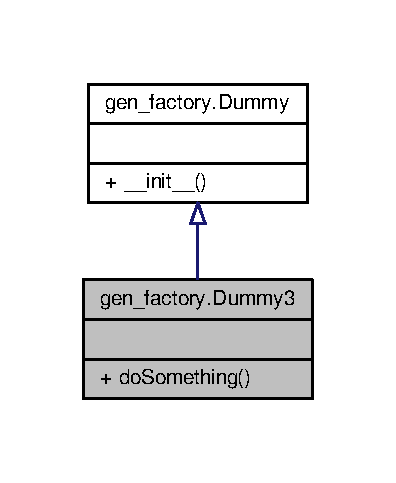
\includegraphics[width=190pt]{classgen__factory_1_1_dummy3__inherit__graph}
\end{center}
\end{figure}


Collaboration diagram for gen\+\_\+factory.\+Dummy3\+:
\nopagebreak
\begin{figure}[H]
\begin{center}
\leavevmode
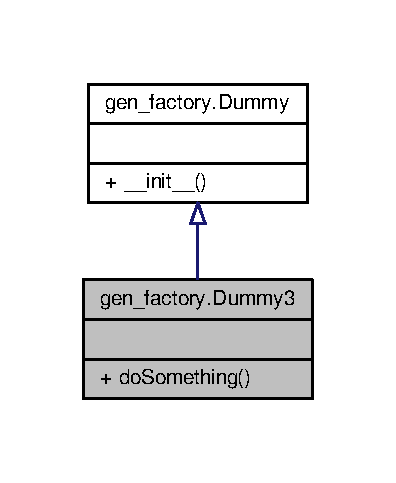
\includegraphics[width=190pt]{classgen__factory_1_1_dummy3__coll__graph}
\end{center}
\end{figure}
\subsection*{Public Member Functions}
\begin{DoxyCompactItemize}
\item 
def \hyperlink{classgen__factory_1_1_dummy3_a7cf07349b2202099fb311e45431bfff4}{do\+Something} (self)
\end{DoxyCompactItemize}


\subsection{Detailed Description}


Definition at line \hyperlink{gen__factory_8py_source_l00028}{28} of file \hyperlink{gen__factory_8py_source}{gen\+\_\+factory.\+py}.



\subsection{Member Function Documentation}
\mbox{\Hypertarget{classgen__factory_1_1_dummy3_a7cf07349b2202099fb311e45431bfff4}\label{classgen__factory_1_1_dummy3_a7cf07349b2202099fb311e45431bfff4}} 
\index{gen\+\_\+factory\+::\+Dummy3@{gen\+\_\+factory\+::\+Dummy3}!do\+Something@{do\+Something}}
\index{do\+Something@{do\+Something}!gen\+\_\+factory\+::\+Dummy3@{gen\+\_\+factory\+::\+Dummy3}}
\subsubsection{\texorpdfstring{do\+Something()}{doSomething()}}
{\footnotesize\ttfamily def gen\+\_\+factory.\+Dummy3.\+do\+Something (\begin{DoxyParamCaption}\item[{}]{self }\end{DoxyParamCaption})}



Definition at line \hyperlink{gen__factory_8py_source_l00029}{29} of file \hyperlink{gen__factory_8py_source}{gen\+\_\+factory.\+py}.


\begin{DoxyCode}
00029     \textcolor{keyword}{def }doSomething (self):
00030         \textcolor{keywordflow}{print} (\textcolor{stringliteral}{"I'm an instance of class \{0\}"}.format (type (self).\_\_name\_\_))
00031 
\end{DoxyCode}


The documentation for this class was generated from the following file\+:\begin{DoxyCompactItemize}
\item 
/home/hilton/github/exch2exh/\hyperlink{gen__factory_8py}{gen\+\_\+factory.\+py}\end{DoxyCompactItemize}

\hypertarget{classexchange_1_1_exchange}{}\section{exchange.\+Exchange Class Reference}
\label{classexchange_1_1_exchange}\index{exchange.\+Exchange@{exchange.\+Exchange}}


Inheritance diagram for exchange.\+Exchange\+:\nopagebreak
\begin{figure}[H]
\begin{center}
\leavevmode
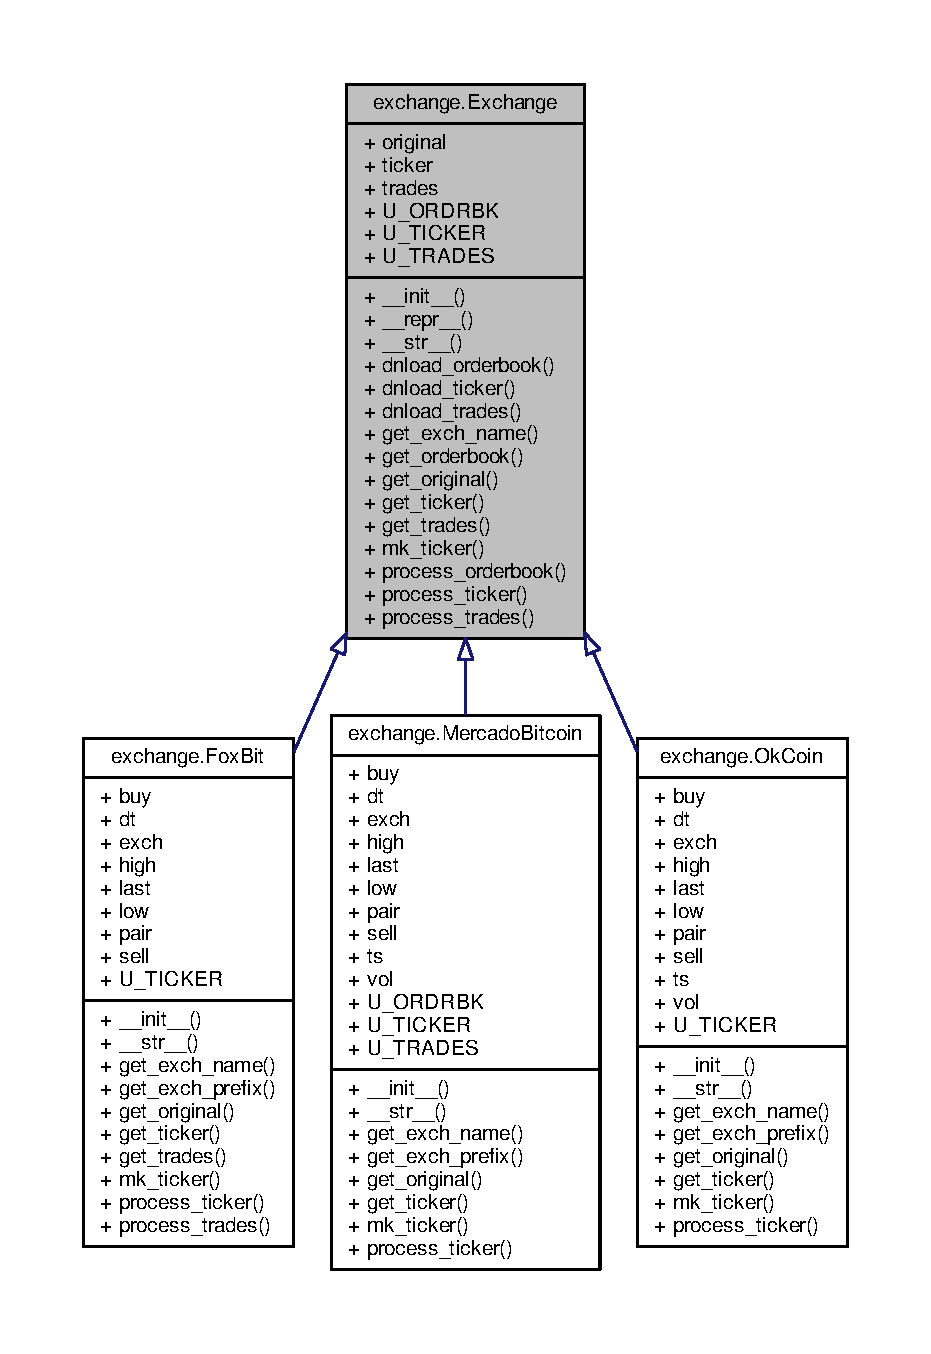
\includegraphics[width=350pt]{classexchange_1_1_exchange__inherit__graph}
\end{center}
\end{figure}


Collaboration diagram for exchange.\+Exchange\+:
\nopagebreak
\begin{figure}[H]
\begin{center}
\leavevmode
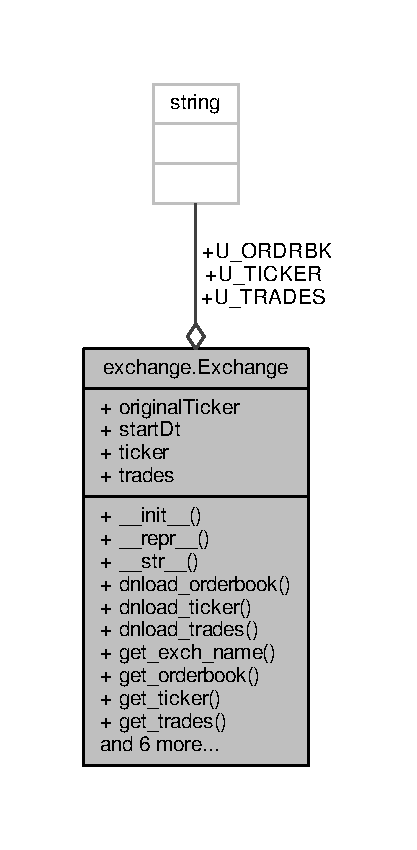
\includegraphics[width=203pt]{classexchange_1_1_exchange__coll__graph}
\end{center}
\end{figure}
\subsection*{Public Member Functions}
\begin{DoxyCompactItemize}
\item 
def \hyperlink{classexchange_1_1_exchange_adc6345bd84ea113d46f4e044dbd4d0fb}{\+\_\+\+\_\+init\+\_\+\+\_\+} (self)
\item 
def \hyperlink{classexchange_1_1_exchange_afff4d01a82947f2e3be0d4fa5e0e0fe7}{\+\_\+\+\_\+repr\+\_\+\+\_\+} (self)
\item 
def \hyperlink{classexchange_1_1_exchange_ae3fd515a25ead8667f917230b0975a98}{\+\_\+\+\_\+str\+\_\+\+\_\+} (self)
\item 
def \hyperlink{classexchange_1_1_exchange_a99f32c746467a00b455a97c7805fd710}{dnload\+\_\+orderbook} (self)
\item 
def \hyperlink{classexchange_1_1_exchange_a9e700d31fd60de495956518436b6768a}{dnload\+\_\+ticker} (self)
\item 
def \hyperlink{classexchange_1_1_exchange_a202c8b57ffa0adcb830de89d6466fd60}{dnload\+\_\+trades} (self)
\item 
def \hyperlink{classexchange_1_1_exchange_a8f095bac98d7ad212f93bfcdff458bf7}{get\+\_\+exch\+\_\+name} (self)
\item 
def \hyperlink{classexchange_1_1_exchange_a5d0c05c289d664892ade5edb03adbd6b}{get\+\_\+orderbook} (self)
\item 
def \hyperlink{classexchange_1_1_exchange_ae7690d173a46bc0f051365ab0b28f81f}{get\+\_\+original} (self)
\item 
def \hyperlink{classexchange_1_1_exchange_aabe7d5679cac0096bc54169cfceea536}{get\+\_\+ticker} (self)
\item 
def \hyperlink{classexchange_1_1_exchange_a254bac1703de55674f5ebfbb03a95e74}{get\+\_\+trades} (self)
\item 
def \hyperlink{classexchange_1_1_exchange_a31c0527e3a8a21fe74f9c24a79a86e6b}{mk\+\_\+ticker} (self)
\item 
def \hyperlink{classexchange_1_1_exchange_a93c60cd18eab808d68191fb1d2d42cf8}{process\+\_\+orderbook} (self)
\item 
def \hyperlink{classexchange_1_1_exchange_aa3f83a45154aa4a1b07010f74c2b37db}{process\+\_\+ticker} (self)
\item 
def \hyperlink{classexchange_1_1_exchange_a0e67454c7053807302be914376790484}{process\+\_\+trades} (self)
\end{DoxyCompactItemize}
\subsection*{Public Attributes}
\begin{DoxyCompactItemize}
\item 
\hyperlink{classexchange_1_1_exchange_af69daf804599e27f7431632d91b2c3b9}{original}
\item 
\hyperlink{classexchange_1_1_exchange_a7cf9e52f993627955a2e242c388daaeb}{ticker}
\item 
\hyperlink{classexchange_1_1_exchange_a30e87a377320ce05bd956fb014683641}{trades}
\end{DoxyCompactItemize}
\subsection*{Static Public Attributes}
\begin{DoxyCompactItemize}
\item 
string \hyperlink{classexchange_1_1_exchange_a83174d2fe96a1c737231d3b8b18d9807}{U\+\_\+\+O\+R\+D\+R\+BK} = \textquotesingle{}\textquotesingle{}
\item 
string \hyperlink{classexchange_1_1_exchange_ab16df02480d727c533b02b5b7afa053b}{U\+\_\+\+T\+I\+C\+K\+ER} = \textquotesingle{}\textquotesingle{}
\item 
string \hyperlink{classexchange_1_1_exchange_aafa0e023de170f51cbf9d48e1154587a}{U\+\_\+\+T\+R\+A\+D\+ES} = \textquotesingle{}\textquotesingle{}
\end{DoxyCompactItemize}


\subsection{Detailed Description}


Definition at line \hyperlink{exchange_8py_source_l00127}{127} of file \hyperlink{exchange_8py_source}{exchange.\+py}.



\subsection{Constructor \& Destructor Documentation}
\index{exchange\+::\+Exchange@{exchange\+::\+Exchange}!\+\_\+\+\_\+init\+\_\+\+\_\+@{\+\_\+\+\_\+init\+\_\+\+\_\+}}
\index{\+\_\+\+\_\+init\+\_\+\+\_\+@{\+\_\+\+\_\+init\+\_\+\+\_\+}!exchange\+::\+Exchange@{exchange\+::\+Exchange}}
\subsubsection[{\texorpdfstring{\+\_\+\+\_\+init\+\_\+\+\_\+(self)}{__init__(self)}}]{\setlength{\rightskip}{0pt plus 5cm}def exchange.\+Exchange.\+\_\+\+\_\+init\+\_\+\+\_\+ (
\begin{DoxyParamCaption}
\item[{}]{self}
\end{DoxyParamCaption}
)}\hypertarget{classexchange_1_1_exchange_adc6345bd84ea113d46f4e044dbd4d0fb}{}\label{classexchange_1_1_exchange_adc6345bd84ea113d46f4e044dbd4d0fb}


Definition at line \hyperlink{exchange_8py_source_l00134}{134} of file \hyperlink{exchange_8py_source}{exchange.\+py}.


\begin{DoxyCode}
\hypertarget{classexchange_1_1_exchange.tex_l00134}{}\hyperlink{classexchange_1_1_exchange_adc6345bd84ea113d46f4e044dbd4d0fb}{00134}     \textcolor{keyword}{def }\hyperlink{classexchange_1_1_exchange_adc6345bd84ea113d46f4e044dbd4d0fb}{\_\_init\_\_} (self):
00135 \textcolor{comment}{#        self.dnload\_ticker ()}
00136 \textcolor{comment}{#        self.process\_ticker ()}
00137         \textcolor{keywordflow}{pass}
00138     
\end{DoxyCode}


\subsection{Member Function Documentation}
\index{exchange\+::\+Exchange@{exchange\+::\+Exchange}!\+\_\+\+\_\+repr\+\_\+\+\_\+@{\+\_\+\+\_\+repr\+\_\+\+\_\+}}
\index{\+\_\+\+\_\+repr\+\_\+\+\_\+@{\+\_\+\+\_\+repr\+\_\+\+\_\+}!exchange\+::\+Exchange@{exchange\+::\+Exchange}}
\subsubsection[{\texorpdfstring{\+\_\+\+\_\+repr\+\_\+\+\_\+(self)}{__repr__(self)}}]{\setlength{\rightskip}{0pt plus 5cm}def exchange.\+Exchange.\+\_\+\+\_\+repr\+\_\+\+\_\+ (
\begin{DoxyParamCaption}
\item[{}]{self}
\end{DoxyParamCaption}
)}\hypertarget{classexchange_1_1_exchange_afff4d01a82947f2e3be0d4fa5e0e0fe7}{}\label{classexchange_1_1_exchange_afff4d01a82947f2e3be0d4fa5e0e0fe7}


Definition at line \hyperlink{exchange_8py_source_l00212}{212} of file \hyperlink{exchange_8py_source}{exchange.\+py}.


\begin{DoxyCode}
\hypertarget{classexchange_1_1_exchange.tex_l00212}{}\hyperlink{classexchange_1_1_exchange_afff4d01a82947f2e3be0d4fa5e0e0fe7}{00212}     \textcolor{keyword}{def }\hyperlink{classexchange_1_1_exchange_afff4d01a82947f2e3be0d4fa5e0e0fe7}{\_\_repr\_\_} (self):
00213         result = \textcolor{stringliteral}{"\{0\} ()"}.format (type (self).\_\_name\_\_)
00214         
00215         \textcolor{comment}{# Normal function termination}
00216         \textcolor{keywordflow}{return} result
00217         
\end{DoxyCode}
\index{exchange\+::\+Exchange@{exchange\+::\+Exchange}!\+\_\+\+\_\+str\+\_\+\+\_\+@{\+\_\+\+\_\+str\+\_\+\+\_\+}}
\index{\+\_\+\+\_\+str\+\_\+\+\_\+@{\+\_\+\+\_\+str\+\_\+\+\_\+}!exchange\+::\+Exchange@{exchange\+::\+Exchange}}
\subsubsection[{\texorpdfstring{\+\_\+\+\_\+str\+\_\+\+\_\+(self)}{__str__(self)}}]{\setlength{\rightskip}{0pt plus 5cm}def exchange.\+Exchange.\+\_\+\+\_\+str\+\_\+\+\_\+ (
\begin{DoxyParamCaption}
\item[{}]{self}
\end{DoxyParamCaption}
)}\hypertarget{classexchange_1_1_exchange_ae3fd515a25ead8667f917230b0975a98}{}\label{classexchange_1_1_exchange_ae3fd515a25ead8667f917230b0975a98}


Definition at line \hyperlink{exchange_8py_source_l00208}{208} of file \hyperlink{exchange_8py_source}{exchange.\+py}.


\begin{DoxyCode}
\hypertarget{classexchange_1_1_exchange.tex_l00208}{}\hyperlink{classexchange_1_1_exchange_ae3fd515a25ead8667f917230b0975a98}{00208}     \textcolor{keyword}{def }\hyperlink{classexchange_1_1_exchange_ae3fd515a25ead8667f917230b0975a98}{\_\_str\_\_} (self):
00209         \textcolor{comment}{# TODO raise exception}
00210         \textcolor{keywordflow}{pass}
00211         
\end{DoxyCode}
\index{exchange\+::\+Exchange@{exchange\+::\+Exchange}!dnload\+\_\+orderbook@{dnload\+\_\+orderbook}}
\index{dnload\+\_\+orderbook@{dnload\+\_\+orderbook}!exchange\+::\+Exchange@{exchange\+::\+Exchange}}
\subsubsection[{\texorpdfstring{dnload\+\_\+orderbook(self)}{dnload_orderbook(self)}}]{\setlength{\rightskip}{0pt plus 5cm}def exchange.\+Exchange.\+dnload\+\_\+orderbook (
\begin{DoxyParamCaption}
\item[{}]{self}
\end{DoxyParamCaption}
)}\hypertarget{classexchange_1_1_exchange_a99f32c746467a00b455a97c7805fd710}{}\label{classexchange_1_1_exchange_a99f32c746467a00b455a97c7805fd710}


Definition at line \hyperlink{exchange_8py_source_l00182}{182} of file \hyperlink{exchange_8py_source}{exchange.\+py}.



References \hyperlink{exchange_8py_source_l00171}{exchange.\+Exchange.\+trades}.


\begin{DoxyCode}
\hypertarget{classexchange_1_1_exchange.tex_l00182}{}\hyperlink{classexchange_1_1_exchange_a99f32c746467a00b455a97c7805fd710}{00182}     \textcolor{keyword}{def }\hyperlink{classexchange_1_1_exchange_a99f32c746467a00b455a97c7805fd710}{dnload\_orderbook} (self):
00183         url = self.\_\_class\_\_.U\_ORDRBK
00184         f = urllib.request.urlopen (url)
00185         
00186         line = f.readline ()
00187 \textcolor{comment}{#        print (line)}
00188         
00189         self.\hyperlink{classexchange_1_1_exchange_a30e87a377320ce05bd956fb014683641}{trades} = json.loads (line.decode (encoding=\textcolor{stringliteral}{'utf-8'}))
00190 \textcolor{comment}{#        print (self.ticker)}
00191         
\end{DoxyCode}
\index{exchange\+::\+Exchange@{exchange\+::\+Exchange}!dnload\+\_\+ticker@{dnload\+\_\+ticker}}
\index{dnload\+\_\+ticker@{dnload\+\_\+ticker}!exchange\+::\+Exchange@{exchange\+::\+Exchange}}
\subsubsection[{\texorpdfstring{dnload\+\_\+ticker(self)}{dnload_ticker(self)}}]{\setlength{\rightskip}{0pt plus 5cm}def exchange.\+Exchange.\+dnload\+\_\+ticker (
\begin{DoxyParamCaption}
\item[{}]{self}
\end{DoxyParamCaption}
)}\hypertarget{classexchange_1_1_exchange_a9e700d31fd60de495956518436b6768a}{}\label{classexchange_1_1_exchange_a9e700d31fd60de495956518436b6768a}


Definition at line \hyperlink{exchange_8py_source_l00139}{139} of file \hyperlink{exchange_8py_source}{exchange.\+py}.


\begin{DoxyCode}
\hypertarget{classexchange_1_1_exchange.tex_l00139}{}\hyperlink{classexchange_1_1_exchange_a9e700d31fd60de495956518436b6768a}{00139}     \textcolor{keyword}{def }\hyperlink{classexchange_1_1_exchange_a9e700d31fd60de495956518436b6768a}{dnload\_ticker} (self):
00140         url = self.\_\_class\_\_.U\_TICKER
00141 \textcolor{comment}{#        print (url)}
00142         f = urllib.request.urlopen (url)
00143         
00144         line = f.readline ()
00145 \textcolor{comment}{#        print (line)}
\hypertarget{classexchange_1_1_exchange.tex_l00146}{}\hyperlink{classexchange_1_1_exchange_af69daf804599e27f7431632d91b2c3b9}{00146}         self.\hyperlink{classexchange_1_1_exchange_af69daf804599e27f7431632d91b2c3b9}{original} = line.decode (encoding = \textcolor{stringliteral}{'utf-8'})
00147         
\hypertarget{classexchange_1_1_exchange.tex_l00148}{}\hyperlink{classexchange_1_1_exchange_a7cf9e52f993627955a2e242c388daaeb}{00148}         self.\hyperlink{classexchange_1_1_exchange_a7cf9e52f993627955a2e242c388daaeb}{ticker} = json.loads (line.decode (encoding=\textcolor{stringliteral}{'utf-8'}))
00149 \textcolor{comment}{#        print (self.ticker)}
00150         
\end{DoxyCode}
\index{exchange\+::\+Exchange@{exchange\+::\+Exchange}!dnload\+\_\+trades@{dnload\+\_\+trades}}
\index{dnload\+\_\+trades@{dnload\+\_\+trades}!exchange\+::\+Exchange@{exchange\+::\+Exchange}}
\subsubsection[{\texorpdfstring{dnload\+\_\+trades(self)}{dnload_trades(self)}}]{\setlength{\rightskip}{0pt plus 5cm}def exchange.\+Exchange.\+dnload\+\_\+trades (
\begin{DoxyParamCaption}
\item[{}]{self}
\end{DoxyParamCaption}
)}\hypertarget{classexchange_1_1_exchange_a202c8b57ffa0adcb830de89d6466fd60}{}\label{classexchange_1_1_exchange_a202c8b57ffa0adcb830de89d6466fd60}


Definition at line \hyperlink{exchange_8py_source_l00163}{163} of file \hyperlink{exchange_8py_source}{exchange.\+py}.


\begin{DoxyCode}
\hypertarget{classexchange_1_1_exchange.tex_l00163}{}\hyperlink{classexchange_1_1_exchange_a202c8b57ffa0adcb830de89d6466fd60}{00163}     \textcolor{keyword}{def }\hyperlink{classexchange_1_1_exchange_a202c8b57ffa0adcb830de89d6466fd60}{dnload\_trades} (self):
00164         url = self.\_\_class\_\_.U\_TRADES
00165 \textcolor{comment}{#        print (url)}
00166         f = urllib.request.urlopen (url)
00167         
00168         line = f.readline ()
00169 \textcolor{comment}{#        print (line)}
00170         
\hypertarget{classexchange_1_1_exchange.tex_l00171}{}\hyperlink{classexchange_1_1_exchange_a30e87a377320ce05bd956fb014683641}{00171}         self.\hyperlink{classexchange_1_1_exchange_a30e87a377320ce05bd956fb014683641}{trades} = json.loads (line.decode (encoding=\textcolor{stringliteral}{'utf-8'}))
00172 \textcolor{comment}{#        print (self.ticker)}
00173         
\end{DoxyCode}
\index{exchange\+::\+Exchange@{exchange\+::\+Exchange}!get\+\_\+exch\+\_\+name@{get\+\_\+exch\+\_\+name}}
\index{get\+\_\+exch\+\_\+name@{get\+\_\+exch\+\_\+name}!exchange\+::\+Exchange@{exchange\+::\+Exchange}}
\subsubsection[{\texorpdfstring{get\+\_\+exch\+\_\+name(self)}{get_exch_name(self)}}]{\setlength{\rightskip}{0pt plus 5cm}def exchange.\+Exchange.\+get\+\_\+exch\+\_\+name (
\begin{DoxyParamCaption}
\item[{}]{self}
\end{DoxyParamCaption}
)}\hypertarget{classexchange_1_1_exchange_a8f095bac98d7ad212f93bfcdff458bf7}{}\label{classexchange_1_1_exchange_a8f095bac98d7ad212f93bfcdff458bf7}


Definition at line \hyperlink{exchange_8py_source_l00200}{200} of file \hyperlink{exchange_8py_source}{exchange.\+py}.


\begin{DoxyCode}
\hypertarget{classexchange_1_1_exchange.tex_l00200}{}\hyperlink{classexchange_1_1_exchange_a8f095bac98d7ad212f93bfcdff458bf7}{00200}     \textcolor{keyword}{def }\hyperlink{classexchange_1_1_exchange_a8f095bac98d7ad212f93bfcdff458bf7}{get\_exch\_name} (self):
00201         \textcolor{comment}{# TODO raise exception}
00202         \textcolor{keywordflow}{pass}
00203     
\end{DoxyCode}
\index{exchange\+::\+Exchange@{exchange\+::\+Exchange}!get\+\_\+orderbook@{get\+\_\+orderbook}}
\index{get\+\_\+orderbook@{get\+\_\+orderbook}!exchange\+::\+Exchange@{exchange\+::\+Exchange}}
\subsubsection[{\texorpdfstring{get\+\_\+orderbook(self)}{get_orderbook(self)}}]{\setlength{\rightskip}{0pt plus 5cm}def exchange.\+Exchange.\+get\+\_\+orderbook (
\begin{DoxyParamCaption}
\item[{}]{self}
\end{DoxyParamCaption}
)}\hypertarget{classexchange_1_1_exchange_a5d0c05c289d664892ade5edb03adbd6b}{}\label{classexchange_1_1_exchange_a5d0c05c289d664892ade5edb03adbd6b}


Definition at line \hyperlink{exchange_8py_source_l00196}{196} of file \hyperlink{exchange_8py_source}{exchange.\+py}.


\begin{DoxyCode}
\hypertarget{classexchange_1_1_exchange.tex_l00196}{}\hyperlink{classexchange_1_1_exchange_a5d0c05c289d664892ade5edb03adbd6b}{00196}     \textcolor{keyword}{def }\hyperlink{classexchange_1_1_exchange_a5d0c05c289d664892ade5edb03adbd6b}{get\_orderbook} (self):
00197         self.\hyperlink{classexchange_1_1_exchange_a99f32c746467a00b455a97c7805fd710}{dnload\_orderbook} ()
00198         self.\hyperlink{classexchange_1_1_exchange_a93c60cd18eab808d68191fb1d2d42cf8}{process\_orderbook} () 
00199     
\end{DoxyCode}


Here is the call graph for this function\+:\nopagebreak
\begin{figure}[H]
\begin{center}
\leavevmode
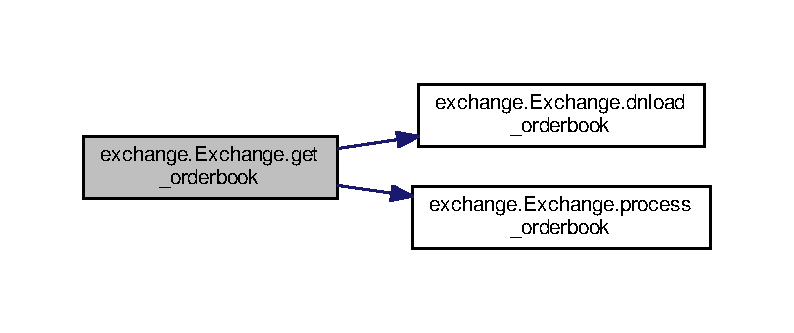
\includegraphics[width=350pt]{classexchange_1_1_exchange_a5d0c05c289d664892ade5edb03adbd6b_cgraph}
\end{center}
\end{figure}


\index{exchange\+::\+Exchange@{exchange\+::\+Exchange}!get\+\_\+original@{get\+\_\+original}}
\index{get\+\_\+original@{get\+\_\+original}!exchange\+::\+Exchange@{exchange\+::\+Exchange}}
\subsubsection[{\texorpdfstring{get\+\_\+original(self)}{get_original(self)}}]{\setlength{\rightskip}{0pt plus 5cm}def exchange.\+Exchange.\+get\+\_\+original (
\begin{DoxyParamCaption}
\item[{}]{self}
\end{DoxyParamCaption}
)}\hypertarget{classexchange_1_1_exchange_ae7690d173a46bc0f051365ab0b28f81f}{}\label{classexchange_1_1_exchange_ae7690d173a46bc0f051365ab0b28f81f}


Definition at line \hyperlink{exchange_8py_source_l00204}{204} of file \hyperlink{exchange_8py_source}{exchange.\+py}.


\begin{DoxyCode}
\hypertarget{classexchange_1_1_exchange.tex_l00204}{}\hyperlink{classexchange_1_1_exchange_ae7690d173a46bc0f051365ab0b28f81f}{00204}     \textcolor{keyword}{def }\hyperlink{classexchange_1_1_exchange_ae7690d173a46bc0f051365ab0b28f81f}{get\_original} (self):
00205         \textcolor{comment}{# TODO raise exception}
00206         \textcolor{keywordflow}{pass}
00207         
\end{DoxyCode}
\index{exchange\+::\+Exchange@{exchange\+::\+Exchange}!get\+\_\+ticker@{get\+\_\+ticker}}
\index{get\+\_\+ticker@{get\+\_\+ticker}!exchange\+::\+Exchange@{exchange\+::\+Exchange}}
\subsubsection[{\texorpdfstring{get\+\_\+ticker(self)}{get_ticker(self)}}]{\setlength{\rightskip}{0pt plus 5cm}def exchange.\+Exchange.\+get\+\_\+ticker (
\begin{DoxyParamCaption}
\item[{}]{self}
\end{DoxyParamCaption}
)}\hypertarget{classexchange_1_1_exchange_aabe7d5679cac0096bc54169cfceea536}{}\label{classexchange_1_1_exchange_aabe7d5679cac0096bc54169cfceea536}


Definition at line \hyperlink{exchange_8py_source_l00155}{155} of file \hyperlink{exchange_8py_source}{exchange.\+py}.


\begin{DoxyCode}
\hypertarget{classexchange_1_1_exchange.tex_l00155}{}\hyperlink{classexchange_1_1_exchange_aabe7d5679cac0096bc54169cfceea536}{00155}     \textcolor{keyword}{def }\hyperlink{classexchange_1_1_exchange_aabe7d5679cac0096bc54169cfceea536}{get\_ticker} (self):
00156         self.\hyperlink{classexchange_1_1_exchange_a9e700d31fd60de495956518436b6768a}{dnload\_ticker} ()
00157         self.\hyperlink{classexchange_1_1_exchange_aa3f83a45154aa4a1b07010f74c2b37db}{process\_ticker} ()
00158     
\end{DoxyCode}


Here is the call graph for this function\+:\nopagebreak
\begin{figure}[H]
\begin{center}
\leavevmode
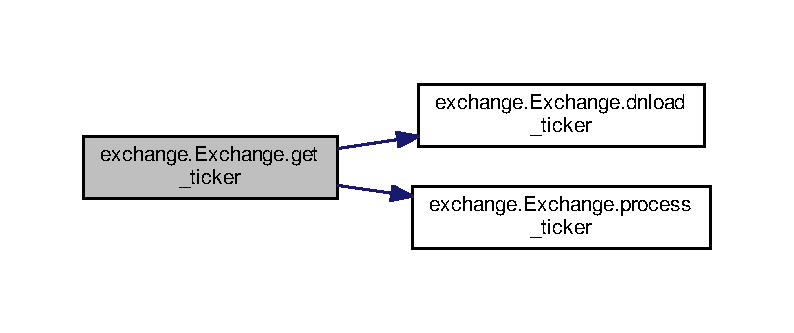
\includegraphics[width=350pt]{classexchange_1_1_exchange_aabe7d5679cac0096bc54169cfceea536_cgraph}
\end{center}
\end{figure}


\index{exchange\+::\+Exchange@{exchange\+::\+Exchange}!get\+\_\+trades@{get\+\_\+trades}}
\index{get\+\_\+trades@{get\+\_\+trades}!exchange\+::\+Exchange@{exchange\+::\+Exchange}}
\subsubsection[{\texorpdfstring{get\+\_\+trades(self)}{get_trades(self)}}]{\setlength{\rightskip}{0pt plus 5cm}def exchange.\+Exchange.\+get\+\_\+trades (
\begin{DoxyParamCaption}
\item[{}]{self}
\end{DoxyParamCaption}
)}\hypertarget{classexchange_1_1_exchange_a254bac1703de55674f5ebfbb03a95e74}{}\label{classexchange_1_1_exchange_a254bac1703de55674f5ebfbb03a95e74}


Definition at line \hyperlink{exchange_8py_source_l00178}{178} of file \hyperlink{exchange_8py_source}{exchange.\+py}.


\begin{DoxyCode}
\hypertarget{classexchange_1_1_exchange.tex_l00178}{}\hyperlink{classexchange_1_1_exchange_a254bac1703de55674f5ebfbb03a95e74}{00178}     \textcolor{keyword}{def }\hyperlink{classexchange_1_1_exchange_a254bac1703de55674f5ebfbb03a95e74}{get\_trades} (self):
00179         self.\hyperlink{classexchange_1_1_exchange_a202c8b57ffa0adcb830de89d6466fd60}{dnload\_trades} ()
00180         self.\hyperlink{classexchange_1_1_exchange_a0e67454c7053807302be914376790484}{process\_trades} ()
00181     
\end{DoxyCode}


Here is the call graph for this function\+:\nopagebreak
\begin{figure}[H]
\begin{center}
\leavevmode
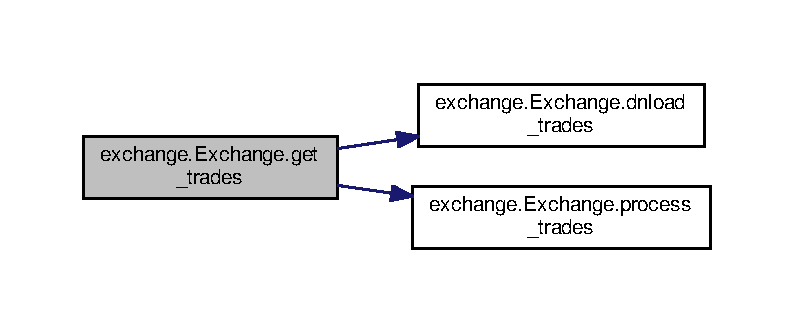
\includegraphics[width=350pt]{classexchange_1_1_exchange_a254bac1703de55674f5ebfbb03a95e74_cgraph}
\end{center}
\end{figure}


\index{exchange\+::\+Exchange@{exchange\+::\+Exchange}!mk\+\_\+ticker@{mk\+\_\+ticker}}
\index{mk\+\_\+ticker@{mk\+\_\+ticker}!exchange\+::\+Exchange@{exchange\+::\+Exchange}}
\subsubsection[{\texorpdfstring{mk\+\_\+ticker(self)}{mk_ticker(self)}}]{\setlength{\rightskip}{0pt plus 5cm}def exchange.\+Exchange.\+mk\+\_\+ticker (
\begin{DoxyParamCaption}
\item[{}]{self}
\end{DoxyParamCaption}
)}\hypertarget{classexchange_1_1_exchange_a31c0527e3a8a21fe74f9c24a79a86e6b}{}\label{classexchange_1_1_exchange_a31c0527e3a8a21fe74f9c24a79a86e6b}


Definition at line \hyperlink{exchange_8py_source_l00159}{159} of file \hyperlink{exchange_8py_source}{exchange.\+py}.


\begin{DoxyCode}
\hypertarget{classexchange_1_1_exchange.tex_l00159}{}\hyperlink{classexchange_1_1_exchange_a31c0527e3a8a21fe74f9c24a79a86e6b}{00159}     \textcolor{keyword}{def }\hyperlink{classexchange_1_1_exchange_a31c0527e3a8a21fe74f9c24a79a86e6b}{mk\_ticker} (self): 
00160         \textcolor{comment}{# TODO raise exception}
00161         \textcolor{keywordflow}{pass}
00162     
\end{DoxyCode}
\index{exchange\+::\+Exchange@{exchange\+::\+Exchange}!process\+\_\+orderbook@{process\+\_\+orderbook}}
\index{process\+\_\+orderbook@{process\+\_\+orderbook}!exchange\+::\+Exchange@{exchange\+::\+Exchange}}
\subsubsection[{\texorpdfstring{process\+\_\+orderbook(self)}{process_orderbook(self)}}]{\setlength{\rightskip}{0pt plus 5cm}def exchange.\+Exchange.\+process\+\_\+orderbook (
\begin{DoxyParamCaption}
\item[{}]{self}
\end{DoxyParamCaption}
)}\hypertarget{classexchange_1_1_exchange_a93c60cd18eab808d68191fb1d2d42cf8}{}\label{classexchange_1_1_exchange_a93c60cd18eab808d68191fb1d2d42cf8}


Definition at line \hyperlink{exchange_8py_source_l00192}{192} of file \hyperlink{exchange_8py_source}{exchange.\+py}.



Referenced by \hyperlink{exchange_8py_source_l00196}{exchange.\+Exchange.\+get\+\_\+orderbook()}.


\begin{DoxyCode}
\hypertarget{classexchange_1_1_exchange.tex_l00192}{}\hyperlink{classexchange_1_1_exchange_a93c60cd18eab808d68191fb1d2d42cf8}{00192}     \textcolor{keyword}{def }\hyperlink{classexchange_1_1_exchange_a93c60cd18eab808d68191fb1d2d42cf8}{process\_orderbook} (self):
00193         \textcolor{comment}{# TODO raise exception}
00194         \textcolor{keywordflow}{pass}
00195     
\end{DoxyCode}


Here is the caller graph for this function\+:\nopagebreak
\begin{figure}[H]
\begin{center}
\leavevmode
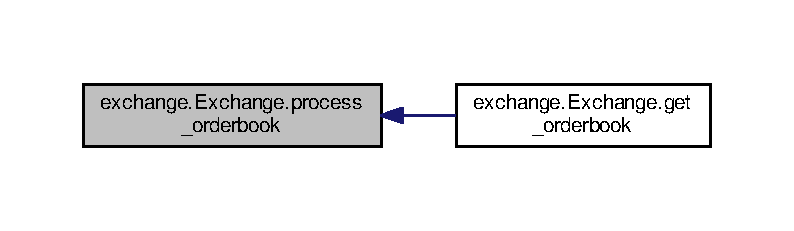
\includegraphics[width=350pt]{classexchange_1_1_exchange_a93c60cd18eab808d68191fb1d2d42cf8_icgraph}
\end{center}
\end{figure}


\index{exchange\+::\+Exchange@{exchange\+::\+Exchange}!process\+\_\+ticker@{process\+\_\+ticker}}
\index{process\+\_\+ticker@{process\+\_\+ticker}!exchange\+::\+Exchange@{exchange\+::\+Exchange}}
\subsubsection[{\texorpdfstring{process\+\_\+ticker(self)}{process_ticker(self)}}]{\setlength{\rightskip}{0pt plus 5cm}def exchange.\+Exchange.\+process\+\_\+ticker (
\begin{DoxyParamCaption}
\item[{}]{self}
\end{DoxyParamCaption}
)}\hypertarget{classexchange_1_1_exchange_aa3f83a45154aa4a1b07010f74c2b37db}{}\label{classexchange_1_1_exchange_aa3f83a45154aa4a1b07010f74c2b37db}


Definition at line \hyperlink{exchange_8py_source_l00151}{151} of file \hyperlink{exchange_8py_source}{exchange.\+py}.



Referenced by \hyperlink{exchange_8py_source_l00155}{exchange.\+Exchange.\+get\+\_\+ticker()}.


\begin{DoxyCode}
\hypertarget{classexchange_1_1_exchange.tex_l00151}{}\hyperlink{classexchange_1_1_exchange_aa3f83a45154aa4a1b07010f74c2b37db}{00151}     \textcolor{keyword}{def }\hyperlink{classexchange_1_1_exchange_aa3f83a45154aa4a1b07010f74c2b37db}{process\_ticker} (self):
00152         \textcolor{comment}{# TODO raise exception}
00153         \textcolor{keywordflow}{pass}
00154     
\end{DoxyCode}


Here is the caller graph for this function\+:\nopagebreak
\begin{figure}[H]
\begin{center}
\leavevmode
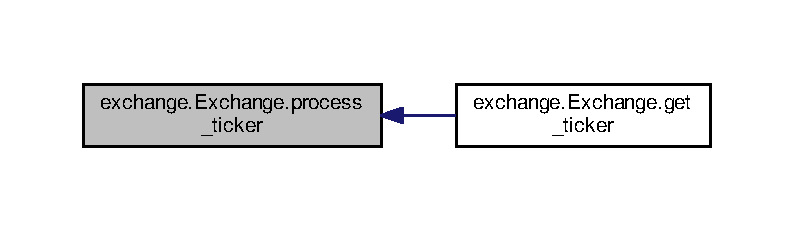
\includegraphics[width=350pt]{classexchange_1_1_exchange_aa3f83a45154aa4a1b07010f74c2b37db_icgraph}
\end{center}
\end{figure}


\index{exchange\+::\+Exchange@{exchange\+::\+Exchange}!process\+\_\+trades@{process\+\_\+trades}}
\index{process\+\_\+trades@{process\+\_\+trades}!exchange\+::\+Exchange@{exchange\+::\+Exchange}}
\subsubsection[{\texorpdfstring{process\+\_\+trades(self)}{process_trades(self)}}]{\setlength{\rightskip}{0pt plus 5cm}def exchange.\+Exchange.\+process\+\_\+trades (
\begin{DoxyParamCaption}
\item[{}]{self}
\end{DoxyParamCaption}
)}\hypertarget{classexchange_1_1_exchange_a0e67454c7053807302be914376790484}{}\label{classexchange_1_1_exchange_a0e67454c7053807302be914376790484}


Definition at line \hyperlink{exchange_8py_source_l00174}{174} of file \hyperlink{exchange_8py_source}{exchange.\+py}.



Referenced by \hyperlink{exchange_8py_source_l00178}{exchange.\+Exchange.\+get\+\_\+trades()}.


\begin{DoxyCode}
\hypertarget{classexchange_1_1_exchange.tex_l00174}{}\hyperlink{classexchange_1_1_exchange_a0e67454c7053807302be914376790484}{00174}     \textcolor{keyword}{def }\hyperlink{classexchange_1_1_exchange_a0e67454c7053807302be914376790484}{process\_trades} (self):
00175         \textcolor{comment}{# TODO raise exception}
00176         \textcolor{keywordflow}{pass}
00177     
\end{DoxyCode}


Here is the caller graph for this function\+:\nopagebreak
\begin{figure}[H]
\begin{center}
\leavevmode
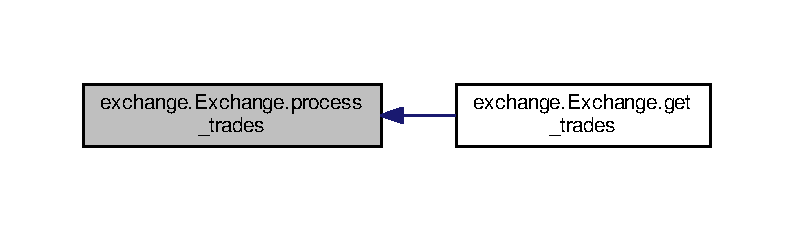
\includegraphics[width=350pt]{classexchange_1_1_exchange_a0e67454c7053807302be914376790484_icgraph}
\end{center}
\end{figure}




\subsection{Member Data Documentation}
\index{exchange\+::\+Exchange@{exchange\+::\+Exchange}!original@{original}}
\index{original@{original}!exchange\+::\+Exchange@{exchange\+::\+Exchange}}
\subsubsection[{\texorpdfstring{original}{original}}]{\setlength{\rightskip}{0pt plus 5cm}exchange.\+Exchange.\+original}\hypertarget{classexchange_1_1_exchange_af69daf804599e27f7431632d91b2c3b9}{}\label{classexchange_1_1_exchange_af69daf804599e27f7431632d91b2c3b9}


Definition at line \hyperlink{exchange_8py_source_l00146}{146} of file \hyperlink{exchange_8py_source}{exchange.\+py}.



Referenced by \hyperlink{exchange_8py_source_l00274}{exchange.\+Fox\+Bit.\+get\+\_\+original()}, \hyperlink{exchange_8py_source_l00343}{exchange.\+Mercado\+Bitcoin.\+get\+\_\+original()}, and \hyperlink{exchange_8py_source_l00402}{exchange.\+Ok\+Coin.\+get\+\_\+original()}.

\index{exchange\+::\+Exchange@{exchange\+::\+Exchange}!ticker@{ticker}}
\index{ticker@{ticker}!exchange\+::\+Exchange@{exchange\+::\+Exchange}}
\subsubsection[{\texorpdfstring{ticker}{ticker}}]{\setlength{\rightskip}{0pt plus 5cm}exchange.\+Exchange.\+ticker}\hypertarget{classexchange_1_1_exchange_a7cf9e52f993627955a2e242c388daaeb}{}\label{classexchange_1_1_exchange_a7cf9e52f993627955a2e242c388daaeb}


Definition at line \hyperlink{exchange_8py_source_l00148}{148} of file \hyperlink{exchange_8py_source}{exchange.\+py}.



Referenced by \hyperlink{exchange_8py_source_l00245}{exchange.\+Fox\+Bit.\+mk\+\_\+ticker()}, and \hyperlink{exchange_8py_source_l00224}{exchange.\+Fox\+Bit.\+process\+\_\+ticker()}.

\index{exchange\+::\+Exchange@{exchange\+::\+Exchange}!trades@{trades}}
\index{trades@{trades}!exchange\+::\+Exchange@{exchange\+::\+Exchange}}
\subsubsection[{\texorpdfstring{trades}{trades}}]{\setlength{\rightskip}{0pt plus 5cm}exchange.\+Exchange.\+trades}\hypertarget{classexchange_1_1_exchange_a30e87a377320ce05bd956fb014683641}{}\label{classexchange_1_1_exchange_a30e87a377320ce05bd956fb014683641}


Definition at line \hyperlink{exchange_8py_source_l00171}{171} of file \hyperlink{exchange_8py_source}{exchange.\+py}.



Referenced by \hyperlink{exchange_8py_source_l00182}{exchange.\+Exchange.\+dnload\+\_\+orderbook()}.

\index{exchange\+::\+Exchange@{exchange\+::\+Exchange}!U\+\_\+\+O\+R\+D\+R\+BK@{U\+\_\+\+O\+R\+D\+R\+BK}}
\index{U\+\_\+\+O\+R\+D\+R\+BK@{U\+\_\+\+O\+R\+D\+R\+BK}!exchange\+::\+Exchange@{exchange\+::\+Exchange}}
\subsubsection[{\texorpdfstring{U\+\_\+\+O\+R\+D\+R\+BK}{U_ORDRBK}}]{\setlength{\rightskip}{0pt plus 5cm}string exchange.\+Exchange.\+U\+\_\+\+O\+R\+D\+R\+BK = \textquotesingle{}\textquotesingle{}\hspace{0.3cm}{\ttfamily [static]}}\hypertarget{classexchange_1_1_exchange_a83174d2fe96a1c737231d3b8b18d9807}{}\label{classexchange_1_1_exchange_a83174d2fe96a1c737231d3b8b18d9807}


Definition at line \hyperlink{exchange_8py_source_l00130}{130} of file \hyperlink{exchange_8py_source}{exchange.\+py}.

\index{exchange\+::\+Exchange@{exchange\+::\+Exchange}!U\+\_\+\+T\+I\+C\+K\+ER@{U\+\_\+\+T\+I\+C\+K\+ER}}
\index{U\+\_\+\+T\+I\+C\+K\+ER@{U\+\_\+\+T\+I\+C\+K\+ER}!exchange\+::\+Exchange@{exchange\+::\+Exchange}}
\subsubsection[{\texorpdfstring{U\+\_\+\+T\+I\+C\+K\+ER}{U_TICKER}}]{\setlength{\rightskip}{0pt plus 5cm}string exchange.\+Exchange.\+U\+\_\+\+T\+I\+C\+K\+ER = \textquotesingle{}\textquotesingle{}\hspace{0.3cm}{\ttfamily [static]}}\hypertarget{classexchange_1_1_exchange_ab16df02480d727c533b02b5b7afa053b}{}\label{classexchange_1_1_exchange_ab16df02480d727c533b02b5b7afa053b}


Definition at line \hyperlink{exchange_8py_source_l00128}{128} of file \hyperlink{exchange_8py_source}{exchange.\+py}.

\index{exchange\+::\+Exchange@{exchange\+::\+Exchange}!U\+\_\+\+T\+R\+A\+D\+ES@{U\+\_\+\+T\+R\+A\+D\+ES}}
\index{U\+\_\+\+T\+R\+A\+D\+ES@{U\+\_\+\+T\+R\+A\+D\+ES}!exchange\+::\+Exchange@{exchange\+::\+Exchange}}
\subsubsection[{\texorpdfstring{U\+\_\+\+T\+R\+A\+D\+ES}{U_TRADES}}]{\setlength{\rightskip}{0pt plus 5cm}string exchange.\+Exchange.\+U\+\_\+\+T\+R\+A\+D\+ES = \textquotesingle{}\textquotesingle{}\hspace{0.3cm}{\ttfamily [static]}}\hypertarget{classexchange_1_1_exchange_aafa0e023de170f51cbf9d48e1154587a}{}\label{classexchange_1_1_exchange_aafa0e023de170f51cbf9d48e1154587a}


Definition at line \hyperlink{exchange_8py_source_l00129}{129} of file \hyperlink{exchange_8py_source}{exchange.\+py}.



The documentation for this class was generated from the following file\+:\begin{DoxyCompactItemize}
\item 
/home/hilton/github/exch2exh/\hyperlink{exchange_8py}{exchange.\+py}\end{DoxyCompactItemize}

\hypertarget{classexchange_1_1_fox_bit}{}\section{exchange.\+Fox\+Bit Class Reference}
\label{classexchange_1_1_fox_bit}\index{exchange.\+Fox\+Bit@{exchange.\+Fox\+Bit}}


Inheritance diagram for exchange.\+Fox\+Bit\+:\nopagebreak
\begin{figure}[H]
\begin{center}
\leavevmode
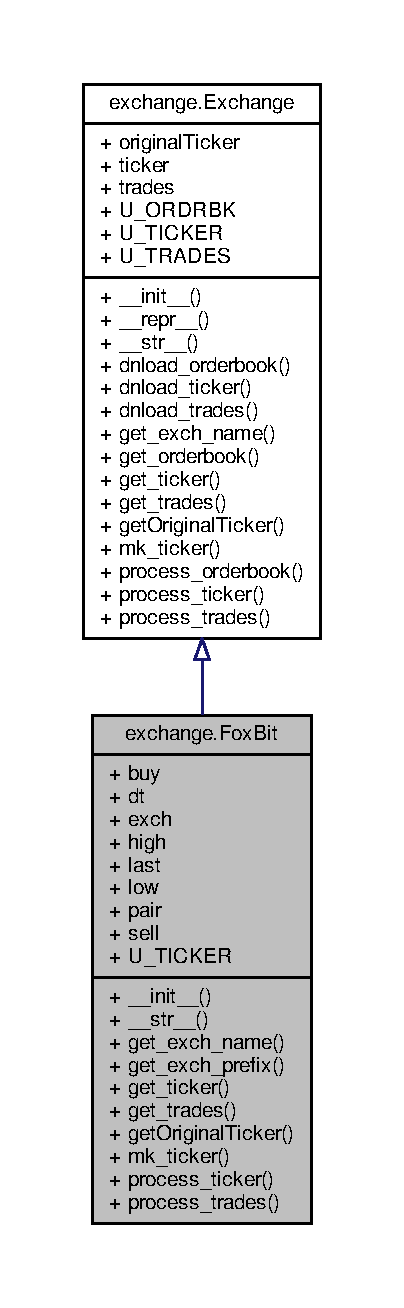
\includegraphics[height=550pt]{classexchange_1_1_fox_bit__inherit__graph}
\end{center}
\end{figure}


Collaboration diagram for exchange.\+Fox\+Bit\+:\nopagebreak
\begin{figure}[H]
\begin{center}
\leavevmode
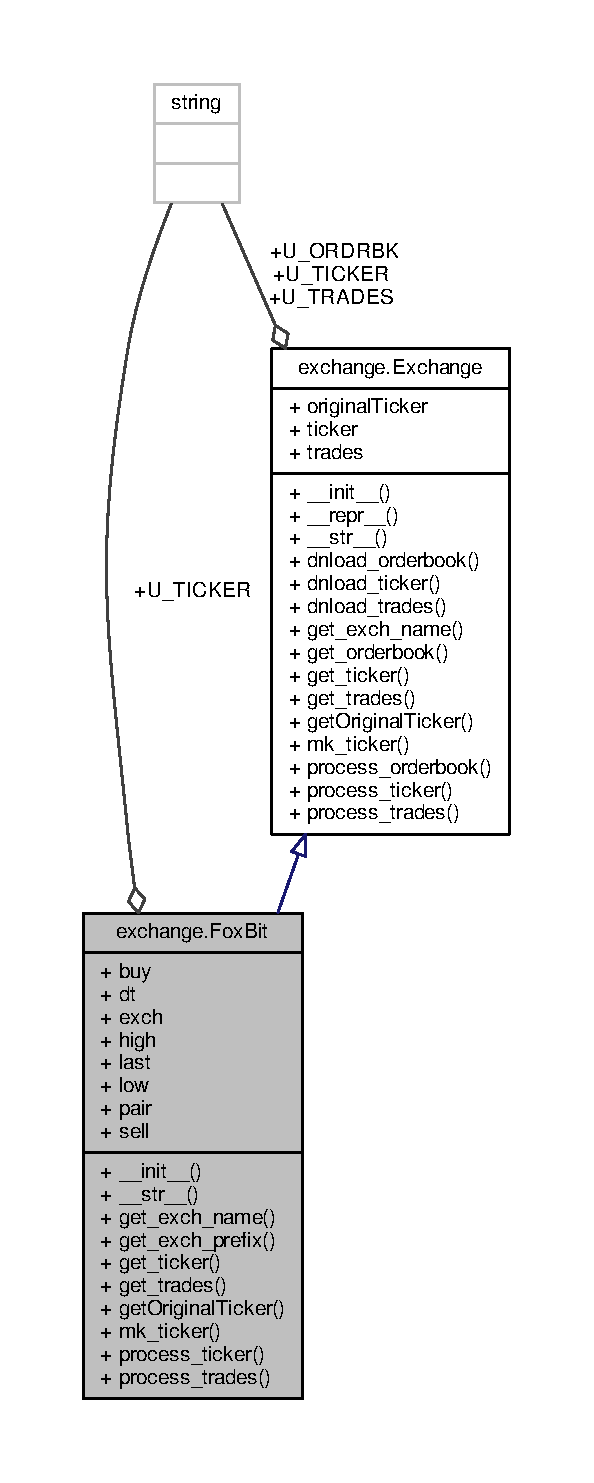
\includegraphics[height=550pt]{classexchange_1_1_fox_bit__coll__graph}
\end{center}
\end{figure}
\subsection*{Public Member Functions}
\begin{DoxyCompactItemize}
\item 
def \hyperlink{classexchange_1_1_fox_bit_a1f892137668748287116d902ef668d1a}{\+\_\+\+\_\+init\+\_\+\+\_\+} (self)
\item 
def \hyperlink{classexchange_1_1_fox_bit_ac21d1d06bf748dfd22ca35bc56a72e3b}{\+\_\+\+\_\+str\+\_\+\+\_\+} (self)
\item 
def \hyperlink{classexchange_1_1_fox_bit_a9bb3b48ee388b422f1d27c1774f0c9bf}{get\+\_\+exch\+\_\+name} (self)
\item 
def \hyperlink{classexchange_1_1_fox_bit_a091fb1b6e76b392b0a018a411f9da200}{get\+\_\+exch\+\_\+prefix} (self)
\item 
def \hyperlink{classexchange_1_1_fox_bit_aeb98818ddef05bb1beff5b55231d3760}{get\+\_\+ticker} (self)
\item 
def \hyperlink{classexchange_1_1_fox_bit_a80807753c2c595997857d097939c9283}{get\+\_\+trades} (self)
\item 
def \hyperlink{classexchange_1_1_fox_bit_adfca60ed33245c7bd9666893f6725bb9}{get\+Original\+Ticker} (self)
\item 
def \hyperlink{classexchange_1_1_fox_bit_a149b379722f351e0b890822a6220f0b0}{mk\+\_\+ticker} (self)
\item 
def \hyperlink{classexchange_1_1_fox_bit_a813481c37754cc0c6e0b1cefa0ec0889}{process\+\_\+ticker} (self)
\item 
def \hyperlink{classexchange_1_1_fox_bit_a244f81e91b04a1118d2d17f6c8497cb5}{process\+\_\+trades} (self)
\end{DoxyCompactItemize}
\subsection*{Public Attributes}
\begin{DoxyCompactItemize}
\item 
\hyperlink{classexchange_1_1_fox_bit_acb7e709cc05e8314b1bdacd32e4dfc80}{buy}
\item 
\hyperlink{classexchange_1_1_fox_bit_a363f8488eb0423f88519c085ae6f168f}{dt}
\item 
\hyperlink{classexchange_1_1_fox_bit_a3922433dcfe54e39c3c0da12fa252658}{exch}
\item 
\hyperlink{classexchange_1_1_fox_bit_a4f6dfaecbcc17ceadddf52d266d9c00d}{high}
\item 
\hyperlink{classexchange_1_1_fox_bit_a5cdbc327b005014dc3b8bb6fb54a12fd}{last}
\item 
\hyperlink{classexchange_1_1_fox_bit_acd666444cff98fe477651120ddb0f915}{low}
\item 
\hyperlink{classexchange_1_1_fox_bit_abfd6daf1cbad94eb74bba4c97fe4a574}{pair}
\item 
\hyperlink{classexchange_1_1_fox_bit_ac1fae4ef7a43254b71d7173a5cc6eeaf}{sell}
\end{DoxyCompactItemize}
\subsection*{Static Public Attributes}
\begin{DoxyCompactItemize}
\item 
string \hyperlink{classexchange_1_1_fox_bit_a7ba3f64a2b55479da2239393c6140ec8}{U\+\_\+\+T\+I\+C\+K\+ER} = \textquotesingle{}https\+://api.\+blinktrade.\+com/api/v1/B\+RL/\hyperlink{classexchange_1_1_exchange_a7cf9e52f993627955a2e242c388daaeb}{ticker}?crypto\+\_\+currency=B\+TC\textquotesingle{}
\end{DoxyCompactItemize}


\subsection{Detailed Description}


Definition at line \hyperlink{exchange_8py_source_l00447}{447} of file \hyperlink{exchange_8py_source}{exchange.\+py}.



\subsection{Constructor \& Destructor Documentation}
\index{exchange\+::\+Fox\+Bit@{exchange\+::\+Fox\+Bit}!\+\_\+\+\_\+init\+\_\+\+\_\+@{\+\_\+\+\_\+init\+\_\+\+\_\+}}
\index{\+\_\+\+\_\+init\+\_\+\+\_\+@{\+\_\+\+\_\+init\+\_\+\+\_\+}!exchange\+::\+Fox\+Bit@{exchange\+::\+Fox\+Bit}}
\subsubsection[{\texorpdfstring{\+\_\+\+\_\+init\+\_\+\+\_\+(self)}{__init__(self)}}]{\setlength{\rightskip}{0pt plus 5cm}def exchange.\+Fox\+Bit.\+\_\+\+\_\+init\+\_\+\+\_\+ (
\begin{DoxyParamCaption}
\item[{}]{self}
\end{DoxyParamCaption}
)}\hypertarget{classexchange_1_1_fox_bit_a1f892137668748287116d902ef668d1a}{}\label{classexchange_1_1_fox_bit_a1f892137668748287116d902ef668d1a}


Definition at line \hyperlink{exchange_8py_source_l00450}{450} of file \hyperlink{exchange_8py_source}{exchange.\+py}.


\begin{DoxyCode}
\hypertarget{classexchange_1_1_fox_bit.tex_l00450}{}\hyperlink{classexchange_1_1_fox_bit_a1f892137668748287116d902ef668d1a}{00450}     \textcolor{keyword}{def }\hyperlink{classexchange_1_1_fox_bit_a1f892137668748287116d902ef668d1a}{\_\_init\_\_} (self):
00451         super ().\_\_init\_\_ ()
00452         
\end{DoxyCode}


\subsection{Member Function Documentation}
\index{exchange\+::\+Fox\+Bit@{exchange\+::\+Fox\+Bit}!\+\_\+\+\_\+str\+\_\+\+\_\+@{\+\_\+\+\_\+str\+\_\+\+\_\+}}
\index{\+\_\+\+\_\+str\+\_\+\+\_\+@{\+\_\+\+\_\+str\+\_\+\+\_\+}!exchange\+::\+Fox\+Bit@{exchange\+::\+Fox\+Bit}}
\subsubsection[{\texorpdfstring{\+\_\+\+\_\+str\+\_\+\+\_\+(self)}{__str__(self)}}]{\setlength{\rightskip}{0pt plus 5cm}def exchange.\+Fox\+Bit.\+\_\+\+\_\+str\+\_\+\+\_\+ (
\begin{DoxyParamCaption}
\item[{}]{self}
\end{DoxyParamCaption}
)}\hypertarget{classexchange_1_1_fox_bit_ac21d1d06bf748dfd22ca35bc56a72e3b}{}\label{classexchange_1_1_fox_bit_ac21d1d06bf748dfd22ca35bc56a72e3b}


Definition at line \hyperlink{exchange_8py_source_l00506}{506} of file \hyperlink{exchange_8py_source}{exchange.\+py}.


\begin{DoxyCode}
\hypertarget{classexchange_1_1_fox_bit.tex_l00506}{}\hyperlink{classexchange_1_1_fox_bit_ac21d1d06bf748dfd22ca35bc56a72e3b}{00506}     \textcolor{keyword}{def }\hyperlink{classexchange_1_1_fox_bit_ac21d1d06bf748dfd22ca35bc56a72e3b}{\_\_str\_\_} (self):
00507         result = json.dumps (self.\_\_dict\_\_, cls = DatetimeEncoder)
00508         
00509         \textcolor{comment}{# Normal function termination}
00510         \textcolor{keywordflow}{return} result
00511                 
\end{DoxyCode}
\index{exchange\+::\+Fox\+Bit@{exchange\+::\+Fox\+Bit}!get\+\_\+exch\+\_\+name@{get\+\_\+exch\+\_\+name}}
\index{get\+\_\+exch\+\_\+name@{get\+\_\+exch\+\_\+name}!exchange\+::\+Fox\+Bit@{exchange\+::\+Fox\+Bit}}
\subsubsection[{\texorpdfstring{get\+\_\+exch\+\_\+name(self)}{get_exch_name(self)}}]{\setlength{\rightskip}{0pt plus 5cm}def exchange.\+Fox\+Bit.\+get\+\_\+exch\+\_\+name (
\begin{DoxyParamCaption}
\item[{}]{self}
\end{DoxyParamCaption}
)}\hypertarget{classexchange_1_1_fox_bit_a9bb3b48ee388b422f1d27c1774f0c9bf}{}\label{classexchange_1_1_fox_bit_a9bb3b48ee388b422f1d27c1774f0c9bf}


Definition at line \hyperlink{exchange_8py_source_l00497}{497} of file \hyperlink{exchange_8py_source}{exchange.\+py}.


\begin{DoxyCode}
\hypertarget{classexchange_1_1_fox_bit.tex_l00497}{}\hyperlink{classexchange_1_1_fox_bit_a9bb3b48ee388b422f1d27c1774f0c9bf}{00497}     \textcolor{keyword}{def }\hyperlink{classexchange_1_1_fox_bit_a9bb3b48ee388b422f1d27c1774f0c9bf}{get\_exch\_name} (self):
00498         \textcolor{keywordflow}{return} \textcolor{stringliteral}{"FoxBit"}
00499     
\end{DoxyCode}
\index{exchange\+::\+Fox\+Bit@{exchange\+::\+Fox\+Bit}!get\+\_\+exch\+\_\+prefix@{get\+\_\+exch\+\_\+prefix}}
\index{get\+\_\+exch\+\_\+prefix@{get\+\_\+exch\+\_\+prefix}!exchange\+::\+Fox\+Bit@{exchange\+::\+Fox\+Bit}}
\subsubsection[{\texorpdfstring{get\+\_\+exch\+\_\+prefix(self)}{get_exch_prefix(self)}}]{\setlength{\rightskip}{0pt plus 5cm}def exchange.\+Fox\+Bit.\+get\+\_\+exch\+\_\+prefix (
\begin{DoxyParamCaption}
\item[{}]{self}
\end{DoxyParamCaption}
)}\hypertarget{classexchange_1_1_fox_bit_a091fb1b6e76b392b0a018a411f9da200}{}\label{classexchange_1_1_fox_bit_a091fb1b6e76b392b0a018a411f9da200}


Definition at line \hyperlink{exchange_8py_source_l00500}{500} of file \hyperlink{exchange_8py_source}{exchange.\+py}.


\begin{DoxyCode}
\hypertarget{classexchange_1_1_fox_bit.tex_l00500}{}\hyperlink{classexchange_1_1_fox_bit_a091fb1b6e76b392b0a018a411f9da200}{00500}     \textcolor{keyword}{def }\hyperlink{classexchange_1_1_fox_bit_a091fb1b6e76b392b0a018a411f9da200}{get\_exch\_prefix} (self):
00501         \textcolor{keywordflow}{return} \textcolor{stringliteral}{"fb"}
00502         
\end{DoxyCode}
\index{exchange\+::\+Fox\+Bit@{exchange\+::\+Fox\+Bit}!get\+\_\+ticker@{get\+\_\+ticker}}
\index{get\+\_\+ticker@{get\+\_\+ticker}!exchange\+::\+Fox\+Bit@{exchange\+::\+Fox\+Bit}}
\subsubsection[{\texorpdfstring{get\+\_\+ticker(self)}{get_ticker(self)}}]{\setlength{\rightskip}{0pt plus 5cm}def exchange.\+Fox\+Bit.\+get\+\_\+ticker (
\begin{DoxyParamCaption}
\item[{}]{self}
\end{DoxyParamCaption}
)}\hypertarget{classexchange_1_1_fox_bit_aeb98818ddef05bb1beff5b55231d3760}{}\label{classexchange_1_1_fox_bit_aeb98818ddef05bb1beff5b55231d3760}


Definition at line \hyperlink{exchange_8py_source_l00460}{460} of file \hyperlink{exchange_8py_source}{exchange.\+py}.


\begin{DoxyCode}
\hypertarget{classexchange_1_1_fox_bit.tex_l00460}{}\hyperlink{classexchange_1_1_fox_bit_aeb98818ddef05bb1beff5b55231d3760}{00460}     \textcolor{keyword}{def }\hyperlink{classexchange_1_1_fox_bit_aeb98818ddef05bb1beff5b55231d3760}{get\_ticker} (self):
00461         super ().get\_ticker ()
00462         
\hypertarget{classexchange_1_1_fox_bit.tex_l00463}{}\hyperlink{classexchange_1_1_fox_bit_a363f8488eb0423f88519c085ae6f168f}{00463}         self.\hyperlink{classexchange_1_1_fox_bit_a363f8488eb0423f88519c085ae6f168f}{dt}   = self.\hyperlink{classexchange_1_1_exchange_a7cf9e52f993627955a2e242c388daaeb}{ticker}[\textcolor{stringliteral}{'date'}]
\hypertarget{classexchange_1_1_fox_bit.tex_l00464}{}\hyperlink{classexchange_1_1_fox_bit_acb7e709cc05e8314b1bdacd32e4dfc80}{00464}         self.\hyperlink{classexchange_1_1_fox_bit_acb7e709cc05e8314b1bdacd32e4dfc80}{buy}  = float (self.\hyperlink{classexchange_1_1_exchange_a7cf9e52f993627955a2e242c388daaeb}{ticker}[\textcolor{stringliteral}{'buy'}])
\hypertarget{classexchange_1_1_fox_bit.tex_l00465}{}\hyperlink{classexchange_1_1_fox_bit_ac1fae4ef7a43254b71d7173a5cc6eeaf}{00465}         self.\hyperlink{classexchange_1_1_fox_bit_ac1fae4ef7a43254b71d7173a5cc6eeaf}{sell} = float (self.\hyperlink{classexchange_1_1_exchange_a7cf9e52f993627955a2e242c388daaeb}{ticker}[\textcolor{stringliteral}{'sell'}])
\hypertarget{classexchange_1_1_fox_bit.tex_l00466}{}\hyperlink{classexchange_1_1_fox_bit_a4f6dfaecbcc17ceadddf52d266d9c00d}{00466}         self.\hyperlink{classexchange_1_1_fox_bit_a4f6dfaecbcc17ceadddf52d266d9c00d}{high} = float (self.\hyperlink{classexchange_1_1_exchange_a7cf9e52f993627955a2e242c388daaeb}{ticker}[\textcolor{stringliteral}{'high'}])
\hypertarget{classexchange_1_1_fox_bit.tex_l00467}{}\hyperlink{classexchange_1_1_fox_bit_acd666444cff98fe477651120ddb0f915}{00467}         self.\hyperlink{classexchange_1_1_fox_bit_acd666444cff98fe477651120ddb0f915}{low}  = float (self.\hyperlink{classexchange_1_1_exchange_a7cf9e52f993627955a2e242c388daaeb}{ticker}[\textcolor{stringliteral}{'low'}])
\hypertarget{classexchange_1_1_fox_bit.tex_l00468}{}\hyperlink{classexchange_1_1_fox_bit_a5cdbc327b005014dc3b8bb6fb54a12fd}{00468}         self.\hyperlink{classexchange_1_1_fox_bit_a5cdbc327b005014dc3b8bb6fb54a12fd}{last} = float (self.\hyperlink{classexchange_1_1_exchange_a7cf9e52f993627955a2e242c388daaeb}{ticker}[\textcolor{stringliteral}{'last'}])
00469         
00470         result = (self.\hyperlink{classexchange_1_1_fox_bit_a363f8488eb0423f88519c085ae6f168f}{dt}, self.\hyperlink{classexchange_1_1_fox_bit_ac1fae4ef7a43254b71d7173a5cc6eeaf}{sell}, self.\hyperlink{classexchange_1_1_fox_bit_acb7e709cc05e8314b1bdacd32e4dfc80}{buy}, self.\hyperlink{classexchange_1_1_fox_bit_a4f6dfaecbcc17ceadddf52d266d9c00d}{high}, self.\hyperlink{classexchange_1_1_fox_bit_acd666444cff98fe477651120ddb0f915}{low}, self.
      \hyperlink{classexchange_1_1_fox_bit_a5cdbc327b005014dc3b8bb6fb54a12fd}{last})
00471         
00472         \textcolor{keywordflow}{return} result
00473     
\end{DoxyCode}
\index{exchange\+::\+Fox\+Bit@{exchange\+::\+Fox\+Bit}!get\+\_\+trades@{get\+\_\+trades}}
\index{get\+\_\+trades@{get\+\_\+trades}!exchange\+::\+Fox\+Bit@{exchange\+::\+Fox\+Bit}}
\subsubsection[{\texorpdfstring{get\+\_\+trades(self)}{get_trades(self)}}]{\setlength{\rightskip}{0pt plus 5cm}def exchange.\+Fox\+Bit.\+get\+\_\+trades (
\begin{DoxyParamCaption}
\item[{}]{self}
\end{DoxyParamCaption}
)}\hypertarget{classexchange_1_1_fox_bit_a80807753c2c595997857d097939c9283}{}\label{classexchange_1_1_fox_bit_a80807753c2c595997857d097939c9283}


Definition at line \hyperlink{exchange_8py_source_l00494}{494} of file \hyperlink{exchange_8py_source}{exchange.\+py}.


\begin{DoxyCode}
\hypertarget{classexchange_1_1_fox_bit.tex_l00494}{}\hyperlink{classexchange_1_1_fox_bit_a80807753c2c595997857d097939c9283}{00494}     \textcolor{keyword}{def }\hyperlink{classexchange_1_1_fox_bit_a80807753c2c595997857d097939c9283}{get\_trades} (self):
00495         \textcolor{keywordflow}{pass}
00496     
\end{DoxyCode}
\index{exchange\+::\+Fox\+Bit@{exchange\+::\+Fox\+Bit}!get\+Original\+Ticker@{get\+Original\+Ticker}}
\index{get\+Original\+Ticker@{get\+Original\+Ticker}!exchange\+::\+Fox\+Bit@{exchange\+::\+Fox\+Bit}}
\subsubsection[{\texorpdfstring{get\+Original\+Ticker(self)}{getOriginalTicker(self)}}]{\setlength{\rightskip}{0pt plus 5cm}def exchange.\+Fox\+Bit.\+get\+Original\+Ticker (
\begin{DoxyParamCaption}
\item[{}]{self}
\end{DoxyParamCaption}
)}\hypertarget{classexchange_1_1_fox_bit_adfca60ed33245c7bd9666893f6725bb9}{}\label{classexchange_1_1_fox_bit_adfca60ed33245c7bd9666893f6725bb9}


Definition at line \hyperlink{exchange_8py_source_l00503}{503} of file \hyperlink{exchange_8py_source}{exchange.\+py}.



References \hyperlink{exchange_8py_source_l00158}{exchange.\+Exchange.\+original\+Ticker}.


\begin{DoxyCode}
\hypertarget{classexchange_1_1_fox_bit.tex_l00503}{}\hyperlink{classexchange_1_1_fox_bit_adfca60ed33245c7bd9666893f6725bb9}{00503}     \textcolor{keyword}{def }\hyperlink{classexchange_1_1_fox_bit_adfca60ed33245c7bd9666893f6725bb9}{getOriginalTicker} (self):
00504         \textcolor{keywordflow}{return} self.\hyperlink{classexchange_1_1_exchange_ae326ce8c325672f3f555af59f22fd9f6}{originalTicker}
00505         
\end{DoxyCode}
\index{exchange\+::\+Fox\+Bit@{exchange\+::\+Fox\+Bit}!mk\+\_\+ticker@{mk\+\_\+ticker}}
\index{mk\+\_\+ticker@{mk\+\_\+ticker}!exchange\+::\+Fox\+Bit@{exchange\+::\+Fox\+Bit}}
\subsubsection[{\texorpdfstring{mk\+\_\+ticker(self)}{mk_ticker(self)}}]{\setlength{\rightskip}{0pt plus 5cm}def exchange.\+Fox\+Bit.\+mk\+\_\+ticker (
\begin{DoxyParamCaption}
\item[{}]{self}
\end{DoxyParamCaption}
)}\hypertarget{classexchange_1_1_fox_bit_a149b379722f351e0b890822a6220f0b0}{}\label{classexchange_1_1_fox_bit_a149b379722f351e0b890822a6220f0b0}


Definition at line \hyperlink{exchange_8py_source_l00474}{474} of file \hyperlink{exchange_8py_source}{exchange.\+py}.



References \hyperlink{exchange_8py_source_l00055}{exchange.\+Ticker.\+exch}, \hyperlink{exch2exch_8py_source_l00064}{exch2exch.\+Xbt\+Prices.\+exch}, \hyperlink{exchange_8py_source_l00317}{exchange.\+Bitfinex.\+exch}, \hyperlink{exchange_8py_source_l00389}{exchange.\+Bitstamp.\+exch}, \hyperlink{exchange_8py_source_l00457}{exchange.\+Fox\+Bit.\+exch}, \hyperlink{exchange_8py_source_l00056}{exchange.\+Ticker.\+pair}, \hyperlink{exchange_8py_source_l00318}{exchange.\+Bitfinex.\+pair}, \hyperlink{exchange_8py_source_l00390}{exchange.\+Bitstamp.\+pair}, \hyperlink{exchange_8py_source_l00458}{exchange.\+Fox\+Bit.\+pair}, and \hyperlink{exchange_8py_source_l00160}{exchange.\+Exchange.\+ticker}.


\begin{DoxyCode}
\hypertarget{classexchange_1_1_fox_bit.tex_l00474}{}\hyperlink{classexchange_1_1_fox_bit_a149b379722f351e0b890822a6220f0b0}{00474}     \textcolor{keyword}{def }\hyperlink{classexchange_1_1_fox_bit_a149b379722f351e0b890822a6220f0b0}{mk\_ticker} (self): 
00475         super ().get\_ticker ()
00476         
00477         exch = self.\hyperlink{classexchange_1_1_fox_bit_a3922433dcfe54e39c3c0da12fa252658}{exch}
00478         pair = self.\hyperlink{classexchange_1_1_fox_bit_abfd6daf1cbad94eb74bba4c97fe4a574}{pair}
00479         ts   = self.\hyperlink{classexchange_1_1_exchange_a7cf9e52f993627955a2e242c388daaeb}{ticker}[\textcolor{stringliteral}{'ts'}]
00480         buy  = float (self.\hyperlink{classexchange_1_1_exchange_a7cf9e52f993627955a2e242c388daaeb}{ticker}[\textcolor{stringliteral}{'buy'}])
00481         sell = float (self.\hyperlink{classexchange_1_1_exchange_a7cf9e52f993627955a2e242c388daaeb}{ticker}[\textcolor{stringliteral}{'sell'}])
00482         high = float (self.\hyperlink{classexchange_1_1_exchange_a7cf9e52f993627955a2e242c388daaeb}{ticker}[\textcolor{stringliteral}{'high'}])
00483         low  = float (self.\hyperlink{classexchange_1_1_exchange_a7cf9e52f993627955a2e242c388daaeb}{ticker}[\textcolor{stringliteral}{'low'}])
00484         last = float (self.\hyperlink{classexchange_1_1_exchange_a7cf9e52f993627955a2e242c388daaeb}{ticker}[\textcolor{stringliteral}{'last'}])
00485         vol  = float (self.\hyperlink{classexchange_1_1_exchange_a7cf9e52f993627955a2e242c388daaeb}{ticker}[\textcolor{stringliteral}{'last'}])
00486         
00487         result = Ticker (exch, pair, ts, buy, sell, high, low, last, vol)
00488         
00489         \textcolor{keywordflow}{return} result
00490         
\end{DoxyCode}
\index{exchange\+::\+Fox\+Bit@{exchange\+::\+Fox\+Bit}!process\+\_\+ticker@{process\+\_\+ticker}}
\index{process\+\_\+ticker@{process\+\_\+ticker}!exchange\+::\+Fox\+Bit@{exchange\+::\+Fox\+Bit}}
\subsubsection[{\texorpdfstring{process\+\_\+ticker(self)}{process_ticker(self)}}]{\setlength{\rightskip}{0pt plus 5cm}def exchange.\+Fox\+Bit.\+process\+\_\+ticker (
\begin{DoxyParamCaption}
\item[{}]{self}
\end{DoxyParamCaption}
)}\hypertarget{classexchange_1_1_fox_bit_a813481c37754cc0c6e0b1cefa0ec0889}{}\label{classexchange_1_1_fox_bit_a813481c37754cc0c6e0b1cefa0ec0889}


Definition at line \hyperlink{exchange_8py_source_l00453}{453} of file \hyperlink{exchange_8py_source}{exchange.\+py}.



References \hyperlink{exchange_8py_source_l00160}{exchange.\+Exchange.\+ticker}.


\begin{DoxyCode}
\hypertarget{classexchange_1_1_fox_bit.tex_l00453}{}\hyperlink{classexchange_1_1_fox_bit_a813481c37754cc0c6e0b1cefa0ec0889}{00453}     \textcolor{keyword}{def }\hyperlink{classexchange_1_1_fox_bit_a813481c37754cc0c6e0b1cefa0ec0889}{process\_ticker} (self):
00454         tt = time.time ()
00455         self.\hyperlink{classexchange_1_1_exchange_a7cf9e52f993627955a2e242c388daaeb}{ticker}[\textcolor{stringliteral}{'ts'}] = tt
00456         self.\hyperlink{classexchange_1_1_exchange_a7cf9e52f993627955a2e242c388daaeb}{ticker}[\textcolor{stringliteral}{'date'}] = datetime.datetime.fromtimestamp (tt)
\hypertarget{classexchange_1_1_fox_bit.tex_l00457}{}\hyperlink{classexchange_1_1_fox_bit_a3922433dcfe54e39c3c0da12fa252658}{00457}         self.\hyperlink{classexchange_1_1_fox_bit_a3922433dcfe54e39c3c0da12fa252658}{exch} = self.\hyperlink{classexchange_1_1_exchange_a8f095bac98d7ad212f93bfcdff458bf7}{get\_exch\_name} ()
\hypertarget{classexchange_1_1_fox_bit.tex_l00458}{}\hyperlink{classexchange_1_1_fox_bit_abfd6daf1cbad94eb74bba4c97fe4a574}{00458}         self.\hyperlink{classexchange_1_1_fox_bit_abfd6daf1cbad94eb74bba4c97fe4a574}{pair} = \textcolor{stringliteral}{"BTCBRL"}
00459      
\end{DoxyCode}
\index{exchange\+::\+Fox\+Bit@{exchange\+::\+Fox\+Bit}!process\+\_\+trades@{process\+\_\+trades}}
\index{process\+\_\+trades@{process\+\_\+trades}!exchange\+::\+Fox\+Bit@{exchange\+::\+Fox\+Bit}}
\subsubsection[{\texorpdfstring{process\+\_\+trades(self)}{process_trades(self)}}]{\setlength{\rightskip}{0pt plus 5cm}def exchange.\+Fox\+Bit.\+process\+\_\+trades (
\begin{DoxyParamCaption}
\item[{}]{self}
\end{DoxyParamCaption}
)}\hypertarget{classexchange_1_1_fox_bit_a244f81e91b04a1118d2d17f6c8497cb5}{}\label{classexchange_1_1_fox_bit_a244f81e91b04a1118d2d17f6c8497cb5}


Definition at line \hyperlink{exchange_8py_source_l00491}{491} of file \hyperlink{exchange_8py_source}{exchange.\+py}.


\begin{DoxyCode}
\hypertarget{classexchange_1_1_fox_bit.tex_l00491}{}\hyperlink{classexchange_1_1_fox_bit_a244f81e91b04a1118d2d17f6c8497cb5}{00491}     \textcolor{keyword}{def }\hyperlink{classexchange_1_1_fox_bit_a244f81e91b04a1118d2d17f6c8497cb5}{process\_trades} (self):
00492         \textcolor{keywordflow}{pass}
00493      
\end{DoxyCode}


\subsection{Member Data Documentation}
\index{exchange\+::\+Fox\+Bit@{exchange\+::\+Fox\+Bit}!buy@{buy}}
\index{buy@{buy}!exchange\+::\+Fox\+Bit@{exchange\+::\+Fox\+Bit}}
\subsubsection[{\texorpdfstring{buy}{buy}}]{\setlength{\rightskip}{0pt plus 5cm}exchange.\+Fox\+Bit.\+buy}\hypertarget{classexchange_1_1_fox_bit_acb7e709cc05e8314b1bdacd32e4dfc80}{}\label{classexchange_1_1_fox_bit_acb7e709cc05e8314b1bdacd32e4dfc80}


Definition at line \hyperlink{exchange_8py_source_l00464}{464} of file \hyperlink{exchange_8py_source}{exchange.\+py}.



Referenced by \hyperlink{raw__urlparser_8py_source_l00074}{raw\+\_\+urlparser.\+Xbt\+Prices.\+\_\+\+\_\+str\+\_\+\+\_\+()}, \hyperlink{exchange_8py_source_l00535}{exchange.\+Mercado\+Bitcoin.\+get\+\_\+ticker()}, \hyperlink{exchange_8py_source_l00600}{exchange.\+Ok\+Coin.\+get\+\_\+ticker()}, \hyperlink{raw__urlparser_8py_source_l00062}{raw\+\_\+urlparser.\+Xbt\+Prices.\+get\+Buy()}, \hyperlink{exchange_8py_source_l00549}{exchange.\+Mercado\+Bitcoin.\+mk\+\_\+ticker()}, and \hyperlink{exchange_8py_source_l00614}{exchange.\+Ok\+Coin.\+mk\+\_\+ticker()}.

\index{exchange\+::\+Fox\+Bit@{exchange\+::\+Fox\+Bit}!dt@{dt}}
\index{dt@{dt}!exchange\+::\+Fox\+Bit@{exchange\+::\+Fox\+Bit}}
\subsubsection[{\texorpdfstring{dt}{dt}}]{\setlength{\rightskip}{0pt plus 5cm}exchange.\+Fox\+Bit.\+dt}\hypertarget{classexchange_1_1_fox_bit_a363f8488eb0423f88519c085ae6f168f}{}\label{classexchange_1_1_fox_bit_a363f8488eb0423f88519c085ae6f168f}


Definition at line \hyperlink{exchange_8py_source_l00463}{463} of file \hyperlink{exchange_8py_source}{exchange.\+py}.



Referenced by \hyperlink{raw__urlparser_8py_source_l00038}{raw\+\_\+urlparser.\+Rates.\+\_\+\+\_\+str\+\_\+\+\_\+()}, \hyperlink{raw__urlparser_8py_source_l00074}{raw\+\_\+urlparser.\+Xbt\+Prices.\+\_\+\+\_\+str\+\_\+\+\_\+()}, \hyperlink{exchange_8py_source_l00535}{exchange.\+Mercado\+Bitcoin.\+get\+\_\+ticker()}, \hyperlink{exchange_8py_source_l00600}{exchange.\+Ok\+Coin.\+get\+\_\+ticker()}, and \hyperlink{raw__urlparser_8py_source_l00059}{raw\+\_\+urlparser.\+Xbt\+Prices.\+get\+Date\+Time()}.

\index{exchange\+::\+Fox\+Bit@{exchange\+::\+Fox\+Bit}!exch@{exch}}
\index{exch@{exch}!exchange\+::\+Fox\+Bit@{exchange\+::\+Fox\+Bit}}
\subsubsection[{\texorpdfstring{exch}{exch}}]{\setlength{\rightskip}{0pt plus 5cm}exchange.\+Fox\+Bit.\+exch}\hypertarget{classexchange_1_1_fox_bit_a3922433dcfe54e39c3c0da12fa252658}{}\label{classexchange_1_1_fox_bit_a3922433dcfe54e39c3c0da12fa252658}


Definition at line \hyperlink{exchange_8py_source_l00457}{457} of file \hyperlink{exchange_8py_source}{exchange.\+py}.



Referenced by \hyperlink{raw__urlparser_8py_source_l00074}{raw\+\_\+urlparser.\+Xbt\+Prices.\+\_\+\+\_\+str\+\_\+\+\_\+()}, \hyperlink{raw__urlparser_8py_source_l00068}{raw\+\_\+urlparser.\+Xbt\+Prices.\+get\+Exchange\+Name()}, \hyperlink{exchange_8py_source_l00474}{exchange.\+Fox\+Bit.\+mk\+\_\+ticker()}, \hyperlink{exchange_8py_source_l00549}{exchange.\+Mercado\+Bitcoin.\+mk\+\_\+ticker()}, and \hyperlink{exchange_8py_source_l00614}{exchange.\+Ok\+Coin.\+mk\+\_\+ticker()}.

\index{exchange\+::\+Fox\+Bit@{exchange\+::\+Fox\+Bit}!high@{high}}
\index{high@{high}!exchange\+::\+Fox\+Bit@{exchange\+::\+Fox\+Bit}}
\subsubsection[{\texorpdfstring{high}{high}}]{\setlength{\rightskip}{0pt plus 5cm}exchange.\+Fox\+Bit.\+high}\hypertarget{classexchange_1_1_fox_bit_a4f6dfaecbcc17ceadddf52d266d9c00d}{}\label{classexchange_1_1_fox_bit_a4f6dfaecbcc17ceadddf52d266d9c00d}


Definition at line \hyperlink{exchange_8py_source_l00466}{466} of file \hyperlink{exchange_8py_source}{exchange.\+py}.



Referenced by \hyperlink{exchange_8py_source_l00535}{exchange.\+Mercado\+Bitcoin.\+get\+\_\+ticker()}, \hyperlink{exchange_8py_source_l00600}{exchange.\+Ok\+Coin.\+get\+\_\+ticker()}, \hyperlink{exchange_8py_source_l00549}{exchange.\+Mercado\+Bitcoin.\+mk\+\_\+ticker()}, and \hyperlink{exchange_8py_source_l00614}{exchange.\+Ok\+Coin.\+mk\+\_\+ticker()}.

\index{exchange\+::\+Fox\+Bit@{exchange\+::\+Fox\+Bit}!last@{last}}
\index{last@{last}!exchange\+::\+Fox\+Bit@{exchange\+::\+Fox\+Bit}}
\subsubsection[{\texorpdfstring{last}{last}}]{\setlength{\rightskip}{0pt plus 5cm}exchange.\+Fox\+Bit.\+last}\hypertarget{classexchange_1_1_fox_bit_a5cdbc327b005014dc3b8bb6fb54a12fd}{}\label{classexchange_1_1_fox_bit_a5cdbc327b005014dc3b8bb6fb54a12fd}


Definition at line \hyperlink{exchange_8py_source_l00468}{468} of file \hyperlink{exchange_8py_source}{exchange.\+py}.



Referenced by \hyperlink{exchange_8py_source_l00535}{exchange.\+Mercado\+Bitcoin.\+get\+\_\+ticker()}, \hyperlink{exchange_8py_source_l00600}{exchange.\+Ok\+Coin.\+get\+\_\+ticker()}, \hyperlink{exchange_8py_source_l00549}{exchange.\+Mercado\+Bitcoin.\+mk\+\_\+ticker()}, and \hyperlink{exchange_8py_source_l00614}{exchange.\+Ok\+Coin.\+mk\+\_\+ticker()}.

\index{exchange\+::\+Fox\+Bit@{exchange\+::\+Fox\+Bit}!low@{low}}
\index{low@{low}!exchange\+::\+Fox\+Bit@{exchange\+::\+Fox\+Bit}}
\subsubsection[{\texorpdfstring{low}{low}}]{\setlength{\rightskip}{0pt plus 5cm}exchange.\+Fox\+Bit.\+low}\hypertarget{classexchange_1_1_fox_bit_acd666444cff98fe477651120ddb0f915}{}\label{classexchange_1_1_fox_bit_acd666444cff98fe477651120ddb0f915}


Definition at line \hyperlink{exchange_8py_source_l00467}{467} of file \hyperlink{exchange_8py_source}{exchange.\+py}.



Referenced by \hyperlink{exchange_8py_source_l00535}{exchange.\+Mercado\+Bitcoin.\+get\+\_\+ticker()}, \hyperlink{exchange_8py_source_l00600}{exchange.\+Ok\+Coin.\+get\+\_\+ticker()}, \hyperlink{exchange_8py_source_l00549}{exchange.\+Mercado\+Bitcoin.\+mk\+\_\+ticker()}, and \hyperlink{exchange_8py_source_l00614}{exchange.\+Ok\+Coin.\+mk\+\_\+ticker()}.

\index{exchange\+::\+Fox\+Bit@{exchange\+::\+Fox\+Bit}!pair@{pair}}
\index{pair@{pair}!exchange\+::\+Fox\+Bit@{exchange\+::\+Fox\+Bit}}
\subsubsection[{\texorpdfstring{pair}{pair}}]{\setlength{\rightskip}{0pt plus 5cm}exchange.\+Fox\+Bit.\+pair}\hypertarget{classexchange_1_1_fox_bit_abfd6daf1cbad94eb74bba4c97fe4a574}{}\label{classexchange_1_1_fox_bit_abfd6daf1cbad94eb74bba4c97fe4a574}


Definition at line \hyperlink{exchange_8py_source_l00458}{458} of file \hyperlink{exchange_8py_source}{exchange.\+py}.



Referenced by \hyperlink{exchange_8py_source_l00474}{exchange.\+Fox\+Bit.\+mk\+\_\+ticker()}, \hyperlink{exchange_8py_source_l00549}{exchange.\+Mercado\+Bitcoin.\+mk\+\_\+ticker()}, and \hyperlink{exchange_8py_source_l00614}{exchange.\+Ok\+Coin.\+mk\+\_\+ticker()}.

\index{exchange\+::\+Fox\+Bit@{exchange\+::\+Fox\+Bit}!sell@{sell}}
\index{sell@{sell}!exchange\+::\+Fox\+Bit@{exchange\+::\+Fox\+Bit}}
\subsubsection[{\texorpdfstring{sell}{sell}}]{\setlength{\rightskip}{0pt plus 5cm}exchange.\+Fox\+Bit.\+sell}\hypertarget{classexchange_1_1_fox_bit_ac1fae4ef7a43254b71d7173a5cc6eeaf}{}\label{classexchange_1_1_fox_bit_ac1fae4ef7a43254b71d7173a5cc6eeaf}


Definition at line \hyperlink{exchange_8py_source_l00465}{465} of file \hyperlink{exchange_8py_source}{exchange.\+py}.



Referenced by \hyperlink{raw__urlparser_8py_source_l00074}{raw\+\_\+urlparser.\+Xbt\+Prices.\+\_\+\+\_\+str\+\_\+\+\_\+()}, \hyperlink{exchange_8py_source_l00535}{exchange.\+Mercado\+Bitcoin.\+get\+\_\+ticker()}, \hyperlink{exchange_8py_source_l00600}{exchange.\+Ok\+Coin.\+get\+\_\+ticker()}, \hyperlink{raw__urlparser_8py_source_l00065}{raw\+\_\+urlparser.\+Xbt\+Prices.\+get\+Sell()}, \hyperlink{exchange_8py_source_l00549}{exchange.\+Mercado\+Bitcoin.\+mk\+\_\+ticker()}, and \hyperlink{exchange_8py_source_l00614}{exchange.\+Ok\+Coin.\+mk\+\_\+ticker()}.

\index{exchange\+::\+Fox\+Bit@{exchange\+::\+Fox\+Bit}!U\+\_\+\+T\+I\+C\+K\+ER@{U\+\_\+\+T\+I\+C\+K\+ER}}
\index{U\+\_\+\+T\+I\+C\+K\+ER@{U\+\_\+\+T\+I\+C\+K\+ER}!exchange\+::\+Fox\+Bit@{exchange\+::\+Fox\+Bit}}
\subsubsection[{\texorpdfstring{U\+\_\+\+T\+I\+C\+K\+ER}{U_TICKER}}]{\setlength{\rightskip}{0pt plus 5cm}string exchange.\+Fox\+Bit.\+U\+\_\+\+T\+I\+C\+K\+ER = \textquotesingle{}https\+://api.\+blinktrade.\+com/api/v1/B\+RL/{\bf ticker}?crypto\+\_\+currency=B\+TC\textquotesingle{}\hspace{0.3cm}{\ttfamily [static]}}\hypertarget{classexchange_1_1_fox_bit_a7ba3f64a2b55479da2239393c6140ec8}{}\label{classexchange_1_1_fox_bit_a7ba3f64a2b55479da2239393c6140ec8}


Definition at line \hyperlink{exchange_8py_source_l00448}{448} of file \hyperlink{exchange_8py_source}{exchange.\+py}.



The documentation for this class was generated from the following file\+:\begin{DoxyCompactItemize}
\item 
/home/hilton/github/exch2exh/\hyperlink{exchange_8py}{exchange.\+py}\end{DoxyCompactItemize}

\hypertarget{classgen__factory_1_1_gen_factory}{}\section{gen\+\_\+factory.\+Gen\+Factory Class Reference}
\label{classgen__factory_1_1_gen_factory}\index{gen\+\_\+factory.\+Gen\+Factory@{gen\+\_\+factory.\+Gen\+Factory}}


Collaboration diagram for gen\+\_\+factory.\+Gen\+Factory\+:
\nopagebreak
\begin{figure}[H]
\begin{center}
\leavevmode
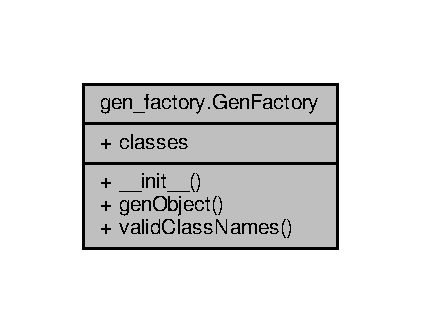
\includegraphics[width=202pt]{classgen__factory_1_1_gen_factory__coll__graph}
\end{center}
\end{figure}
\subsection*{Public Member Functions}
\begin{DoxyCompactItemize}
\item 
def \hyperlink{classgen__factory_1_1_gen_factory_a519ddaf62a8d97e9ee0624e91ac39368}{\+\_\+\+\_\+init\+\_\+\+\_\+} (self, cls)
\item 
def \hyperlink{classgen__factory_1_1_gen_factory_aeb00856af2fa15d7973be43678779561}{gen\+Object} (self, name)
\item 
def \hyperlink{classgen__factory_1_1_gen_factory_ae778039c093668c28d6ea32c92ff082c}{is\+Valid\+Class\+Name} (self, class\+Name)
\item 
def \hyperlink{classgen__factory_1_1_gen_factory_aafa5db7ad22687c37e6b6a73da52fb2f}{valid\+Class\+Names} (self)
\end{DoxyCompactItemize}
\subsection*{Public Attributes}
\begin{DoxyCompactItemize}
\item 
\hyperlink{classgen__factory_1_1_gen_factory_a7a23dc95968c745a9570a42e8e331232}{case\+Significant}
\item 
\hyperlink{classgen__factory_1_1_gen_factory_a28f3142219cbe573169e5f90508908b3}{classes}
\item 
\hyperlink{classgen__factory_1_1_gen_factory_ad263a87721215cc90b4b36e06a258a41}{class\+Names}
\end{DoxyCompactItemize}


\subsection{Detailed Description}


Definition at line \hyperlink{gen__factory_8py_source_l00032}{32} of file \hyperlink{gen__factory_8py_source}{gen\+\_\+factory.\+py}.



\subsection{Constructor \& Destructor Documentation}
\mbox{\Hypertarget{classgen__factory_1_1_gen_factory_a519ddaf62a8d97e9ee0624e91ac39368}\label{classgen__factory_1_1_gen_factory_a519ddaf62a8d97e9ee0624e91ac39368}} 
\index{gen\+\_\+factory\+::\+Gen\+Factory@{gen\+\_\+factory\+::\+Gen\+Factory}!\+\_\+\+\_\+init\+\_\+\+\_\+@{\+\_\+\+\_\+init\+\_\+\+\_\+}}
\index{\+\_\+\+\_\+init\+\_\+\+\_\+@{\+\_\+\+\_\+init\+\_\+\+\_\+}!gen\+\_\+factory\+::\+Gen\+Factory@{gen\+\_\+factory\+::\+Gen\+Factory}}
\subsubsection{\texorpdfstring{\+\_\+\+\_\+init\+\_\+\+\_\+()}{\_\_init\_\_()}}
{\footnotesize\ttfamily def gen\+\_\+factory.\+Gen\+Factory.\+\_\+\+\_\+init\+\_\+\+\_\+ (\begin{DoxyParamCaption}\item[{}]{self,  }\item[{}]{cls }\end{DoxyParamCaption})}



Definition at line \hyperlink{gen__factory_8py_source_l00033}{33} of file \hyperlink{gen__factory_8py_source}{gen\+\_\+factory.\+py}.


\begin{DoxyCode}
00033     \textcolor{keyword}{def }\hyperlink{namespacestart__time_a9c9bd378729a13c96a22c8b079ea172c}{\_\_init\_\_} (self, cls):
00034         types = cls.\_\_subclasses\_\_ ()
00035         
00036 \textcolor{comment}{#        print (self.types)}
00037         
00038         self.classes = \{\}
00039         classNames = []
00040         \textcolor{keywordflow}{for} cls \textcolor{keywordflow}{in} types:
00041             name = cls.\_\_name\_\_
00042             self.classes[name] = cls
00043             classNames.append (name.lower ())
00044             
00045         self.caseSignificant = \textcolor{keyword}{False}
00046         
00047         hasDuplicates = \textcolor{keyword}{False}
00048         classNames.sort ()
00049         \textcolor{keywordflow}{for} ind \textcolor{keywordflow}{in} range (len (classNames) - 1):
00050             \textcolor{keywordflow}{if} classNames[ind] == classNames[ind]:
00051                 hasDuplicates = \textcolor{keyword}{True}
00052                 \textcolor{keywordflow}{break}
00053         
00054         \textcolor{keywordflow}{if} hasDuplicates:
00055             self.caseSignificant = \textcolor{keyword}{True}
00056             self.classNames = self.classes.keys ()
00057             
00058         \textcolor{keywordflow}{else}:
00059             self.classNames = classNames
00060             
00061             
\end{DoxyCode}


\subsection{Member Function Documentation}
\mbox{\Hypertarget{classgen__factory_1_1_gen_factory_aeb00856af2fa15d7973be43678779561}\label{classgen__factory_1_1_gen_factory_aeb00856af2fa15d7973be43678779561}} 
\index{gen\+\_\+factory\+::\+Gen\+Factory@{gen\+\_\+factory\+::\+Gen\+Factory}!gen\+Object@{gen\+Object}}
\index{gen\+Object@{gen\+Object}!gen\+\_\+factory\+::\+Gen\+Factory@{gen\+\_\+factory\+::\+Gen\+Factory}}
\subsubsection{\texorpdfstring{gen\+Object()}{genObject()}}
{\footnotesize\ttfamily def gen\+\_\+factory.\+Gen\+Factory.\+gen\+Object (\begin{DoxyParamCaption}\item[{}]{self,  }\item[{}]{name }\end{DoxyParamCaption})}



Definition at line \hyperlink{gen__factory_8py_source_l00072}{72} of file \hyperlink{gen__factory_8py_source}{gen\+\_\+factory.\+py}.



References \hyperlink{gen__factory_8py_source_l00038}{gen\+\_\+factory.\+Gen\+Factory.\+classes}.


\begin{DoxyCode}
00072     \textcolor{keyword}{def }genObject (self, name):
00073         result = \textcolor{keywordtype}{None} 
00074         
00075         \textcolor{keywordflow}{if} name \textcolor{keywordflow}{in} self.classes:
00076                 cls = self.classes[name]
00077                 result = cls.\_\_new\_\_ (cls)
00078                 
00079                 result.\_\_init\_\_ ()
00080                 
00081         \textcolor{keywordflow}{return} result
00082     
00083         
\end{DoxyCode}
\mbox{\Hypertarget{classgen__factory_1_1_gen_factory_ae778039c093668c28d6ea32c92ff082c}\label{classgen__factory_1_1_gen_factory_ae778039c093668c28d6ea32c92ff082c}} 
\index{gen\+\_\+factory\+::\+Gen\+Factory@{gen\+\_\+factory\+::\+Gen\+Factory}!is\+Valid\+Class\+Name@{is\+Valid\+Class\+Name}}
\index{is\+Valid\+Class\+Name@{is\+Valid\+Class\+Name}!gen\+\_\+factory\+::\+Gen\+Factory@{gen\+\_\+factory\+::\+Gen\+Factory}}
\subsubsection{\texorpdfstring{is\+Valid\+Class\+Name()}{isValidClassName()}}
{\footnotesize\ttfamily def gen\+\_\+factory.\+Gen\+Factory.\+is\+Valid\+Class\+Name (\begin{DoxyParamCaption}\item[{}]{self,  }\item[{}]{class\+Name }\end{DoxyParamCaption})}



Definition at line \hyperlink{gen__factory_8py_source_l00065}{65} of file \hyperlink{gen__factory_8py_source}{gen\+\_\+factory.\+py}.



References \hyperlink{gen__factory_8py_source_l00045}{gen\+\_\+factory.\+Gen\+Factory.\+case\+Significant}, and \hyperlink{gen__factory_8py_source_l00056}{gen\+\_\+factory.\+Gen\+Factory.\+class\+Names}.


\begin{DoxyCode}
00065     \textcolor{keyword}{def }isValidClassName (self, className):
00066         \textcolor{keywordflow}{if} \textcolor{keywordflow}{not} self.caseSignificant:
00067             className = className.lower ()
00068         
00069         \textcolor{comment}{# Normal function termination}
00070         \textcolor{keywordflow}{return} (className \textcolor{keywordflow}{in} self.classNames)
00071     
\end{DoxyCode}
\mbox{\Hypertarget{classgen__factory_1_1_gen_factory_aafa5db7ad22687c37e6b6a73da52fb2f}\label{classgen__factory_1_1_gen_factory_aafa5db7ad22687c37e6b6a73da52fb2f}} 
\index{gen\+\_\+factory\+::\+Gen\+Factory@{gen\+\_\+factory\+::\+Gen\+Factory}!valid\+Class\+Names@{valid\+Class\+Names}}
\index{valid\+Class\+Names@{valid\+Class\+Names}!gen\+\_\+factory\+::\+Gen\+Factory@{gen\+\_\+factory\+::\+Gen\+Factory}}
\subsubsection{\texorpdfstring{valid\+Class\+Names()}{validClassNames()}}
{\footnotesize\ttfamily def gen\+\_\+factory.\+Gen\+Factory.\+valid\+Class\+Names (\begin{DoxyParamCaption}\item[{}]{self }\end{DoxyParamCaption})}



Definition at line \hyperlink{gen__factory_8py_source_l00062}{62} of file \hyperlink{gen__factory_8py_source}{gen\+\_\+factory.\+py}.



References \hyperlink{gen__factory_8py_source_l00038}{gen\+\_\+factory.\+Gen\+Factory.\+classes}.


\begin{DoxyCode}
00062     \textcolor{keyword}{def }validClassNames (self):
00063         \textcolor{keywordflow}{return} self.classes.keys ()
00064     
\end{DoxyCode}


\subsection{Member Data Documentation}
\mbox{\Hypertarget{classgen__factory_1_1_gen_factory_a7a23dc95968c745a9570a42e8e331232}\label{classgen__factory_1_1_gen_factory_a7a23dc95968c745a9570a42e8e331232}} 
\index{gen\+\_\+factory\+::\+Gen\+Factory@{gen\+\_\+factory\+::\+Gen\+Factory}!case\+Significant@{case\+Significant}}
\index{case\+Significant@{case\+Significant}!gen\+\_\+factory\+::\+Gen\+Factory@{gen\+\_\+factory\+::\+Gen\+Factory}}
\subsubsection{\texorpdfstring{case\+Significant}{caseSignificant}}
{\footnotesize\ttfamily gen\+\_\+factory.\+Gen\+Factory.\+case\+Significant}



Definition at line \hyperlink{gen__factory_8py_source_l00045}{45} of file \hyperlink{gen__factory_8py_source}{gen\+\_\+factory.\+py}.



Referenced by \hyperlink{gen__factory_8py_source_l00065}{gen\+\_\+factory.\+Gen\+Factory.\+is\+Valid\+Class\+Name()}.

\mbox{\Hypertarget{classgen__factory_1_1_gen_factory_a28f3142219cbe573169e5f90508908b3}\label{classgen__factory_1_1_gen_factory_a28f3142219cbe573169e5f90508908b3}} 
\index{gen\+\_\+factory\+::\+Gen\+Factory@{gen\+\_\+factory\+::\+Gen\+Factory}!classes@{classes}}
\index{classes@{classes}!gen\+\_\+factory\+::\+Gen\+Factory@{gen\+\_\+factory\+::\+Gen\+Factory}}
\subsubsection{\texorpdfstring{classes}{classes}}
{\footnotesize\ttfamily gen\+\_\+factory.\+Gen\+Factory.\+classes}



Definition at line \hyperlink{gen__factory_8py_source_l00038}{38} of file \hyperlink{gen__factory_8py_source}{gen\+\_\+factory.\+py}.



Referenced by \hyperlink{gen__factory_8py_source_l00072}{gen\+\_\+factory.\+Gen\+Factory.\+gen\+Object()}, and \hyperlink{gen__factory_8py_source_l00062}{gen\+\_\+factory.\+Gen\+Factory.\+valid\+Class\+Names()}.

\mbox{\Hypertarget{classgen__factory_1_1_gen_factory_ad263a87721215cc90b4b36e06a258a41}\label{classgen__factory_1_1_gen_factory_ad263a87721215cc90b4b36e06a258a41}} 
\index{gen\+\_\+factory\+::\+Gen\+Factory@{gen\+\_\+factory\+::\+Gen\+Factory}!class\+Names@{class\+Names}}
\index{class\+Names@{class\+Names}!gen\+\_\+factory\+::\+Gen\+Factory@{gen\+\_\+factory\+::\+Gen\+Factory}}
\subsubsection{\texorpdfstring{class\+Names}{classNames}}
{\footnotesize\ttfamily gen\+\_\+factory.\+Gen\+Factory.\+class\+Names}



Definition at line \hyperlink{gen__factory_8py_source_l00056}{56} of file \hyperlink{gen__factory_8py_source}{gen\+\_\+factory.\+py}.



Referenced by \hyperlink{gen__factory_8py_source_l00065}{gen\+\_\+factory.\+Gen\+Factory.\+is\+Valid\+Class\+Name()}.



The documentation for this class was generated from the following file\+:\begin{DoxyCompactItemize}
\item 
/home/hilton/github/exch2exh/\hyperlink{gen__factory_8py}{gen\+\_\+factory.\+py}\end{DoxyCompactItemize}

\hypertarget{classrates_1_1_google}{}\section{rates.\+Google Class Reference}
\label{classrates_1_1_google}\index{rates.\+Google@{rates.\+Google}}


Inheritance diagram for rates.\+Google\+:\nopagebreak
\begin{figure}[H]
\begin{center}
\leavevmode
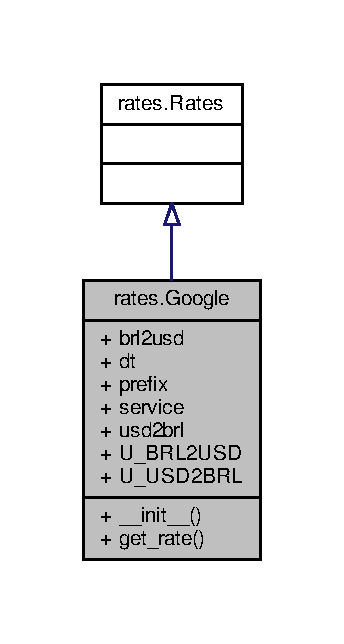
\includegraphics[width=165pt]{classrates_1_1_google__inherit__graph}
\end{center}
\end{figure}


Collaboration diagram for rates.\+Google\+:\nopagebreak
\begin{figure}[H]
\begin{center}
\leavevmode
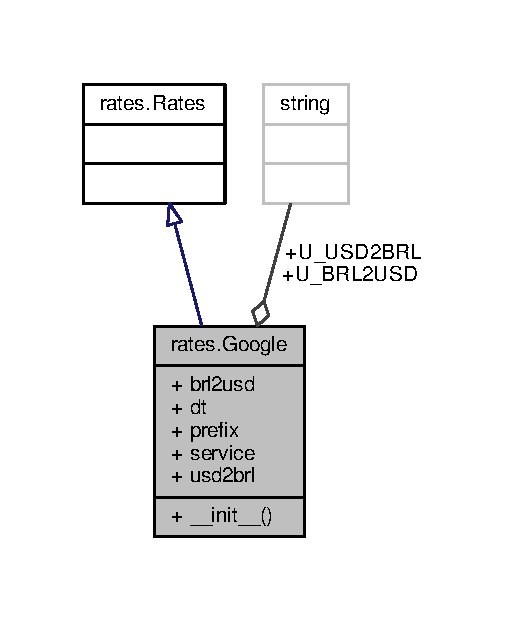
\includegraphics[width=243pt]{classrates_1_1_google__coll__graph}
\end{center}
\end{figure}
\subsection*{Public Member Functions}
\begin{DoxyCompactItemize}
\item 
def \hyperlink{classrates_1_1_google_a6d9d023db3b4f6f2b585397e3469c396}{\+\_\+\+\_\+init\+\_\+\+\_\+} (self)
\item 
def \hyperlink{classrates_1_1_google_afa49252959b89741449dca773f2141b8}{get\+\_\+rate} (url)
\end{DoxyCompactItemize}
\subsection*{Public Attributes}
\begin{DoxyCompactItemize}
\item 
\hyperlink{classrates_1_1_google_a0979ffcb18b8bf3156cc5735c67ca6df}{brl2usd}
\item 
\hyperlink{classrates_1_1_google_a76574be36237f78780f76bed53e69ab2}{dt}
\item 
\hyperlink{classrates_1_1_google_ada5de8700ad571d0ab819fa0163d6bbe}{prefix}
\item 
\hyperlink{classrates_1_1_google_a1da08e36d5007aa5293d048b625a35e9}{service}
\item 
\hyperlink{classrates_1_1_google_a94c28f6d60d5d6afc075416d7378471c}{usd2brl}
\end{DoxyCompactItemize}
\subsection*{Static Public Attributes}
\begin{DoxyCompactItemize}
\item 
string \hyperlink{classrates_1_1_google_a46dbc3fa0a110bf5b66808c29642cfa1}{U\+\_\+\+B\+R\+L2\+U\+SD} = \textquotesingle{}https\+://finance.\+google.\+com/finance/converter?a=1\&from=B\+RL\&to=U\+SD\&meta=ei\%3\+D\+Yqi6\+Wej-\/\+Aoy\+Eeo\+Lbh9g\+F\textquotesingle{}
\item 
string \hyperlink{classrates_1_1_google_a77ef7f5932c48b002697fb187a234d4a}{U\+\_\+\+U\+S\+D2\+B\+RL} = \textquotesingle{}https\+://finance.\+google.\+com/finance/converter?a=1\&from=U\+SD\&to=B\+RL\&meta=ei\%3\+Do\+Ki6\+Wfn\+P\+As\+S\+Teo\+K\+No\+J\+A\+B\textquotesingle{}
\end{DoxyCompactItemize}


\subsection{Detailed Description}


Definition at line \hyperlink{rates_8py_source_l00051}{51} of file \hyperlink{rates_8py_source}{rates.\+py}.



\subsection{Constructor \& Destructor Documentation}
\index{rates\+::\+Google@{rates\+::\+Google}!\+\_\+\+\_\+init\+\_\+\+\_\+@{\+\_\+\+\_\+init\+\_\+\+\_\+}}
\index{\+\_\+\+\_\+init\+\_\+\+\_\+@{\+\_\+\+\_\+init\+\_\+\+\_\+}!rates\+::\+Google@{rates\+::\+Google}}
\subsubsection[{\texorpdfstring{\+\_\+\+\_\+init\+\_\+\+\_\+(self)}{__init__(self)}}]{\setlength{\rightskip}{0pt plus 5cm}def rates.\+Google.\+\_\+\+\_\+init\+\_\+\+\_\+ (
\begin{DoxyParamCaption}
\item[{}]{self}
\end{DoxyParamCaption}
)}\hypertarget{classrates_1_1_google_a6d9d023db3b4f6f2b585397e3469c396}{}\label{classrates_1_1_google_a6d9d023db3b4f6f2b585397e3469c396}


Definition at line \hyperlink{rates_8py_source_l00087}{87} of file \hyperlink{rates_8py_source}{rates.\+py}.


\begin{DoxyCode}
\hypertarget{classrates_1_1_google.tex_l00087}{}\hyperlink{classrates_1_1_google_a6d9d023db3b4f6f2b585397e3469c396}{00087}     \textcolor{keyword}{def }\hyperlink{classrates_1_1_google_a6d9d023db3b4f6f2b585397e3469c396}{\_\_init\_\_} (self):
00088         ts = math.trunc (time.time () + 0.5)
\hypertarget{classrates_1_1_google.tex_l00089}{}\hyperlink{classrates_1_1_google_a76574be36237f78780f76bed53e69ab2}{00089}         self.\hyperlink{classrates_1_1_google_a76574be36237f78780f76bed53e69ab2}{dt} = datetime.datetime.fromtimestamp (ts)
00090                 
\hypertarget{classrates_1_1_google.tex_l00091}{}\hyperlink{classrates_1_1_google_a94c28f6d60d5d6afc075416d7378471c}{00091}         self.\hyperlink{classrates_1_1_google_a94c28f6d60d5d6afc075416d7378471c}{usd2brl} = Google.get\_rate (Google.U\_USD2BRL)
\hypertarget{classrates_1_1_google.tex_l00092}{}\hyperlink{classrates_1_1_google_a0979ffcb18b8bf3156cc5735c67ca6df}{00092}         self.\hyperlink{classrates_1_1_google_a0979ffcb18b8bf3156cc5735c67ca6df}{brl2usd} = Google.get\_rate (Google.U\_BRL2USD)
00093                 
\hypertarget{classrates_1_1_google.tex_l00094}{}\hyperlink{classrates_1_1_google_a1da08e36d5007aa5293d048b625a35e9}{00094}         self.\hyperlink{classrates_1_1_google_a1da08e36d5007aa5293d048b625a35e9}{service} = \textcolor{stringliteral}{"Google"}
\hypertarget{classrates_1_1_google.tex_l00095}{}\hyperlink{classrates_1_1_google_ada5de8700ad571d0ab819fa0163d6bbe}{00095}         self.\hyperlink{classrates_1_1_google_ada5de8700ad571d0ab819fa0163d6bbe}{prefix} = \textcolor{stringliteral}{"ggl"}
00096                 
00097         \textcolor{comment}{# Normal function termination}
00098         \textcolor{keywordflow}{return}
00099             
\end{DoxyCode}


\subsection{Member Function Documentation}
\index{rates\+::\+Google@{rates\+::\+Google}!get\+\_\+rate@{get\+\_\+rate}}
\index{get\+\_\+rate@{get\+\_\+rate}!rates\+::\+Google@{rates\+::\+Google}}
\subsubsection[{\texorpdfstring{get\+\_\+rate(url)}{get_rate(url)}}]{\setlength{\rightskip}{0pt plus 5cm}def rates.\+Google.\+get\+\_\+rate (
\begin{DoxyParamCaption}
\item[{}]{url}
\end{DoxyParamCaption}
)}\hypertarget{classrates_1_1_google_afa49252959b89741449dca773f2141b8}{}\label{classrates_1_1_google_afa49252959b89741449dca773f2141b8}


Definition at line \hyperlink{rates_8py_source_l00057}{57} of file \hyperlink{rates_8py_source}{rates.\+py}.


\begin{DoxyCode}
\hypertarget{classrates_1_1_google.tex_l00057}{}\hyperlink{classrates_1_1_google_afa49252959b89741449dca773f2141b8}{00057}     \textcolor{keyword}{def }\hyperlink{classrates_1_1_google_afa49252959b89741449dca773f2141b8}{get\_rate} (url):
00058         result = 0
00059     
00060         f = urllib.request.urlopen (url)
00061         
00062         \textcolor{keywordflow}{try}:
00063             line = f.readline ()
00064             \textcolor{keywordflow}{while} line != b\textcolor{stringliteral}{''}:
00065                 ind = line.find (b\textcolor{stringliteral}{'currency\_converter'})
00066                 \textcolor{keywordflow}{if} ind != -1:
00067                     
00068                     fields = line.split ()
00069                     rate = fields[5].split (b\textcolor{stringliteral}{'>'})[1]
00070                     
00071                     \textcolor{keywordflow}{break}
00072                     
00073                 line = f.readline ()
00074             
00075             result = float (rate)
00076         \textcolor{keywordflow}{except} IndexError \textcolor{keyword}{as} err:
00077             result = 0.0
00078             
00079             fmt = \textcolor{stringliteral}{"Google.get\_rate(): \{0\}"}
00080             \textcolor{keywordflow}{print} (fmt.format (err))
00081             
00082             \textcolor{keywordflow}{raise}
00083         
00084         \textcolor{comment}{# Normal function termination}
00085         \textcolor{keywordflow}{return} result
00086 
\end{DoxyCode}


\subsection{Member Data Documentation}
\index{rates\+::\+Google@{rates\+::\+Google}!brl2usd@{brl2usd}}
\index{brl2usd@{brl2usd}!rates\+::\+Google@{rates\+::\+Google}}
\subsubsection[{\texorpdfstring{brl2usd}{brl2usd}}]{\setlength{\rightskip}{0pt plus 5cm}rates.\+Google.\+brl2usd}\hypertarget{classrates_1_1_google_a0979ffcb18b8bf3156cc5735c67ca6df}{}\label{classrates_1_1_google_a0979ffcb18b8bf3156cc5735c67ca6df}


Definition at line \hyperlink{rates_8py_source_l00092}{92} of file \hyperlink{rates_8py_source}{rates.\+py}.



Referenced by \hyperlink{raw__urlparser_8py_source_l00038}{raw\+\_\+urlparser.\+Rates.\+\_\+\+\_\+str\+\_\+\+\_\+()}, and \hyperlink{raw__urlparser_8py_source_l00029}{raw\+\_\+urlparser.\+Rates.\+get\+Brl2\+Usd()}.

\index{rates\+::\+Google@{rates\+::\+Google}!dt@{dt}}
\index{dt@{dt}!rates\+::\+Google@{rates\+::\+Google}}
\subsubsection[{\texorpdfstring{dt}{dt}}]{\setlength{\rightskip}{0pt plus 5cm}rates.\+Google.\+dt}\hypertarget{classrates_1_1_google_a76574be36237f78780f76bed53e69ab2}{}\label{classrates_1_1_google_a76574be36237f78780f76bed53e69ab2}


Definition at line \hyperlink{rates_8py_source_l00089}{89} of file \hyperlink{rates_8py_source}{rates.\+py}.



Referenced by \hyperlink{raw__urlparser_8py_source_l00038}{raw\+\_\+urlparser.\+Rates.\+\_\+\+\_\+str\+\_\+\+\_\+()}, \hyperlink{raw__urlparser_8py_source_l00074}{raw\+\_\+urlparser.\+Xbt\+Prices.\+\_\+\+\_\+str\+\_\+\+\_\+()}, and \hyperlink{raw__urlparser_8py_source_l00059}{raw\+\_\+urlparser.\+Xbt\+Prices.\+get\+Date\+Time()}.

\index{rates\+::\+Google@{rates\+::\+Google}!prefix@{prefix}}
\index{prefix@{prefix}!rates\+::\+Google@{rates\+::\+Google}}
\subsubsection[{\texorpdfstring{prefix}{prefix}}]{\setlength{\rightskip}{0pt plus 5cm}rates.\+Google.\+prefix}\hypertarget{classrates_1_1_google_ada5de8700ad571d0ab819fa0163d6bbe}{}\label{classrates_1_1_google_ada5de8700ad571d0ab819fa0163d6bbe}


Definition at line \hyperlink{rates_8py_source_l00095}{95} of file \hyperlink{rates_8py_source}{rates.\+py}.

\index{rates\+::\+Google@{rates\+::\+Google}!service@{service}}
\index{service@{service}!rates\+::\+Google@{rates\+::\+Google}}
\subsubsection[{\texorpdfstring{service}{service}}]{\setlength{\rightskip}{0pt plus 5cm}rates.\+Google.\+service}\hypertarget{classrates_1_1_google_a1da08e36d5007aa5293d048b625a35e9}{}\label{classrates_1_1_google_a1da08e36d5007aa5293d048b625a35e9}


Definition at line \hyperlink{rates_8py_source_l00094}{94} of file \hyperlink{rates_8py_source}{rates.\+py}.



Referenced by \hyperlink{raw__urlparser_8py_source_l00038}{raw\+\_\+urlparser.\+Rates.\+\_\+\+\_\+str\+\_\+\+\_\+()}, and \hyperlink{raw__urlparser_8py_source_l00035}{raw\+\_\+urlparser.\+Rates.\+get\+Service\+Name()}.

\index{rates\+::\+Google@{rates\+::\+Google}!U\+\_\+\+B\+R\+L2\+U\+SD@{U\+\_\+\+B\+R\+L2\+U\+SD}}
\index{U\+\_\+\+B\+R\+L2\+U\+SD@{U\+\_\+\+B\+R\+L2\+U\+SD}!rates\+::\+Google@{rates\+::\+Google}}
\subsubsection[{\texorpdfstring{U\+\_\+\+B\+R\+L2\+U\+SD}{U_BRL2USD}}]{\setlength{\rightskip}{0pt plus 5cm}string rates.\+Google.\+U\+\_\+\+B\+R\+L2\+U\+SD = \textquotesingle{}https\+://finance.\+google.\+com/finance/converter?a=1\&from=B\+RL\&to=U\+SD\&meta=ei\%3\+D\+Yqi6\+Wej-\/\+Aoy\+Eeo\+Lbh9g\+F\textquotesingle{}\hspace{0.3cm}{\ttfamily [static]}}\hypertarget{classrates_1_1_google_a46dbc3fa0a110bf5b66808c29642cfa1}{}\label{classrates_1_1_google_a46dbc3fa0a110bf5b66808c29642cfa1}


Definition at line \hyperlink{rates_8py_source_l00055}{55} of file \hyperlink{rates_8py_source}{rates.\+py}.

\index{rates\+::\+Google@{rates\+::\+Google}!U\+\_\+\+U\+S\+D2\+B\+RL@{U\+\_\+\+U\+S\+D2\+B\+RL}}
\index{U\+\_\+\+U\+S\+D2\+B\+RL@{U\+\_\+\+U\+S\+D2\+B\+RL}!rates\+::\+Google@{rates\+::\+Google}}
\subsubsection[{\texorpdfstring{U\+\_\+\+U\+S\+D2\+B\+RL}{U_USD2BRL}}]{\setlength{\rightskip}{0pt plus 5cm}string rates.\+Google.\+U\+\_\+\+U\+S\+D2\+B\+RL = \textquotesingle{}https\+://finance.\+google.\+com/finance/converter?a=1\&from=U\+SD\&to=B\+RL\&meta=ei\%3\+Do\+Ki6\+Wfn\+P\+As\+S\+Teo\+K\+No\+J\+A\+B\textquotesingle{}\hspace{0.3cm}{\ttfamily [static]}}\hypertarget{classrates_1_1_google_a77ef7f5932c48b002697fb187a234d4a}{}\label{classrates_1_1_google_a77ef7f5932c48b002697fb187a234d4a}


Definition at line \hyperlink{rates_8py_source_l00053}{53} of file \hyperlink{rates_8py_source}{rates.\+py}.

\index{rates\+::\+Google@{rates\+::\+Google}!usd2brl@{usd2brl}}
\index{usd2brl@{usd2brl}!rates\+::\+Google@{rates\+::\+Google}}
\subsubsection[{\texorpdfstring{usd2brl}{usd2brl}}]{\setlength{\rightskip}{0pt plus 5cm}rates.\+Google.\+usd2brl}\hypertarget{classrates_1_1_google_a94c28f6d60d5d6afc075416d7378471c}{}\label{classrates_1_1_google_a94c28f6d60d5d6afc075416d7378471c}


Definition at line \hyperlink{rates_8py_source_l00091}{91} of file \hyperlink{rates_8py_source}{rates.\+py}.



Referenced by \hyperlink{raw__urlparser_8py_source_l00038}{raw\+\_\+urlparser.\+Rates.\+\_\+\+\_\+str\+\_\+\+\_\+()}, and \hyperlink{raw__urlparser_8py_source_l00032}{raw\+\_\+urlparser.\+Rates.\+get\+Usd2\+Brl()}.



The documentation for this class was generated from the following file\+:\begin{DoxyCompactItemize}
\item 
/home/hilton/github/exch2exh/\hyperlink{rates_8py}{rates.\+py}\end{DoxyCompactItemize}

\hypertarget{classexchange_1_1_mercado_bitcoin}{}\section{exchange.\+Mercado\+Bitcoin Class Reference}
\label{classexchange_1_1_mercado_bitcoin}\index{exchange.\+Mercado\+Bitcoin@{exchange.\+Mercado\+Bitcoin}}


Inheritance diagram for exchange.\+Mercado\+Bitcoin\+:\nopagebreak
\begin{figure}[H]
\begin{center}
\leavevmode
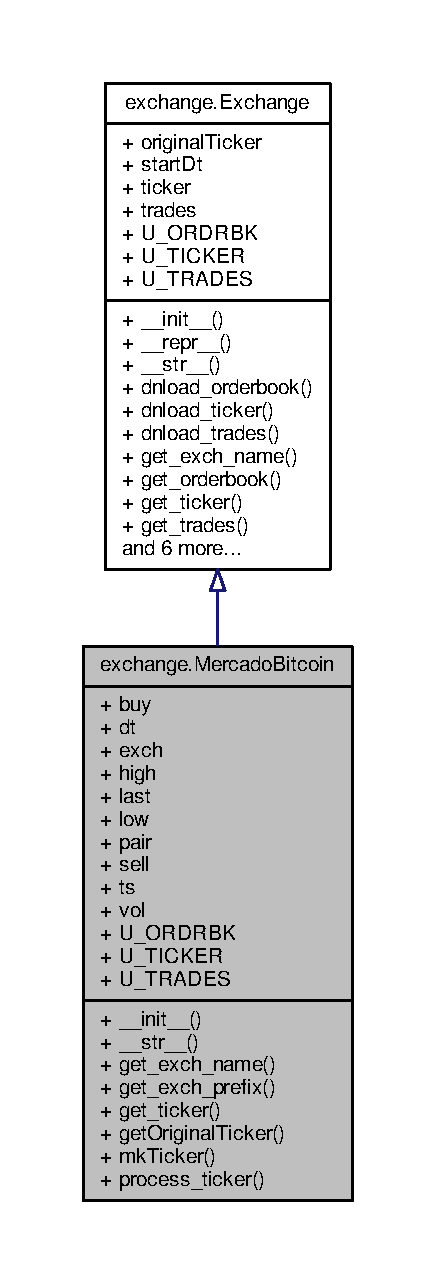
\includegraphics[height=550pt]{classexchange_1_1_mercado_bitcoin__inherit__graph}
\end{center}
\end{figure}


Collaboration diagram for exchange.\+Mercado\+Bitcoin\+:\nopagebreak
\begin{figure}[H]
\begin{center}
\leavevmode
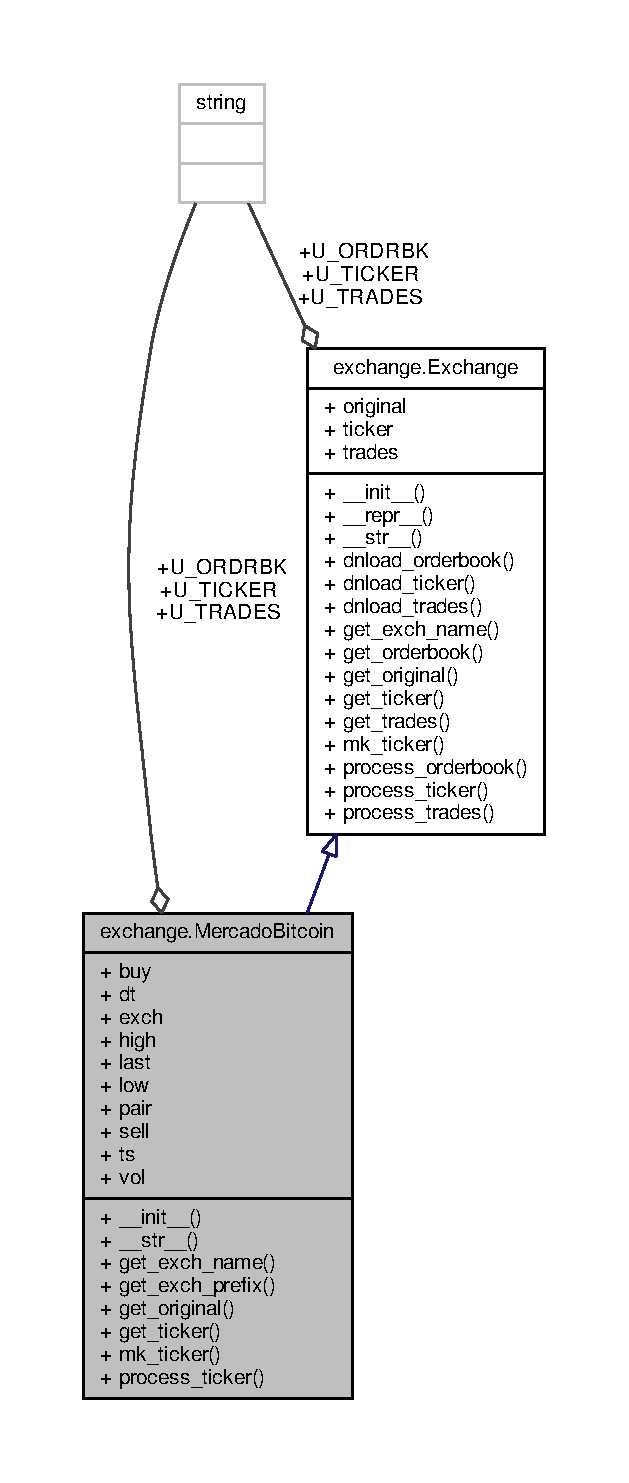
\includegraphics[height=550pt]{classexchange_1_1_mercado_bitcoin__coll__graph}
\end{center}
\end{figure}
\subsection*{Public Member Functions}
\begin{DoxyCompactItemize}
\item 
def \hyperlink{classexchange_1_1_mercado_bitcoin_a7ae88346e48e6e1fa70ebe3281ba7357}{\+\_\+\+\_\+init\+\_\+\+\_\+} (self)
\item 
def \hyperlink{classexchange_1_1_mercado_bitcoin_a42dd78e0cca02c3ab3c185545a879b26}{\+\_\+\+\_\+str\+\_\+\+\_\+} (self)
\item 
def \hyperlink{classexchange_1_1_mercado_bitcoin_a0d7b9201247f88f3013e83fd8e8012d0}{get\+\_\+exch\+\_\+name} (self)
\item 
def \hyperlink{classexchange_1_1_mercado_bitcoin_a61500a3a404e9dc0279717d1d2de85f4}{get\+\_\+exch\+\_\+prefix} (self)
\item 
def \hyperlink{classexchange_1_1_mercado_bitcoin_a2e6fe3e59daf6791688af7ed15772452}{get\+\_\+ticker} (self)
\item 
def \hyperlink{classexchange_1_1_mercado_bitcoin_a1f65e187370684cf17076eb8d0e126d2}{get\+Original\+Ticker} (self)
\item 
def \hyperlink{classexchange_1_1_mercado_bitcoin_a5c2280e8efc3dd148d724e9b73bd9243}{mk\+\_\+ticker} (self)
\item 
def \hyperlink{classexchange_1_1_mercado_bitcoin_a2acc4c0710269e72bc9547508be97117}{process\+\_\+ticker} (self)
\end{DoxyCompactItemize}
\subsection*{Public Attributes}
\begin{DoxyCompactItemize}
\item 
\hyperlink{classexchange_1_1_mercado_bitcoin_ada27b62a35286b9f5dbb54590c5bacd2}{buy}
\item 
\hyperlink{classexchange_1_1_mercado_bitcoin_aeee983ba4f72223a11fb914d22902c56}{dt}
\item 
\hyperlink{classexchange_1_1_mercado_bitcoin_a68701550b43374441e52ea2082d88400}{exch}
\item 
\hyperlink{classexchange_1_1_mercado_bitcoin_a0b9c2d465601a48e3b8838354e931c39}{high}
\item 
\hyperlink{classexchange_1_1_mercado_bitcoin_a5f2759cd17d5dd36bc813c815543f3cc}{last}
\item 
\hyperlink{classexchange_1_1_mercado_bitcoin_aaa3aae824bfc5ba3b7dc5252e9554713}{low}
\item 
\hyperlink{classexchange_1_1_mercado_bitcoin_a879f8ca352d313230d72e6e8785985a1}{pair}
\item 
\hyperlink{classexchange_1_1_mercado_bitcoin_a9982c7a3f6103c88c64160a5854c35cd}{sell}
\item 
\hyperlink{classexchange_1_1_mercado_bitcoin_ac4630b08e08f9eeb9dad838dc9dc0cda}{ts}
\item 
\hyperlink{classexchange_1_1_mercado_bitcoin_a1c163489086ba85b960db821117cd433}{vol}
\end{DoxyCompactItemize}
\subsection*{Static Public Attributes}
\begin{DoxyCompactItemize}
\item 
string \hyperlink{classexchange_1_1_mercado_bitcoin_a7dd22c2c0261557a694678d8057d2547}{U\+\_\+\+O\+R\+D\+R\+BK} = \textquotesingle{}https\+://www.\+mercadobitcoin.\+net/api/B\+TC/orderbook/\textquotesingle{}
\item 
string \hyperlink{classexchange_1_1_mercado_bitcoin_a310b7df5ae9e8a46bad918428c67d4e8}{U\+\_\+\+T\+I\+C\+K\+ER} = \textquotesingle{}https\+://www.\+mercadobitcoin.\+net/api/\hyperlink{classexchange_1_1_exchange_a7cf9e52f993627955a2e242c388daaeb}{ticker}/\textquotesingle{}
\item 
string \hyperlink{classexchange_1_1_mercado_bitcoin_a20ad6407ef07ab8a55d3c022d1512a5d}{U\+\_\+\+T\+R\+A\+D\+ES} = \textquotesingle{}https\+://www.\+mercadobitcoin.\+net/api/B\+TC/\hyperlink{classexchange_1_1_exchange_a30e87a377320ce05bd956fb014683641}{trades}/\textquotesingle{}
\end{DoxyCompactItemize}


\subsection{Detailed Description}


Definition at line \hyperlink{exchange_8py_source_l00520}{520} of file \hyperlink{exchange_8py_source}{exchange.\+py}.



\subsection{Constructor \& Destructor Documentation}
\index{exchange\+::\+Mercado\+Bitcoin@{exchange\+::\+Mercado\+Bitcoin}!\+\_\+\+\_\+init\+\_\+\+\_\+@{\+\_\+\+\_\+init\+\_\+\+\_\+}}
\index{\+\_\+\+\_\+init\+\_\+\+\_\+@{\+\_\+\+\_\+init\+\_\+\+\_\+}!exchange\+::\+Mercado\+Bitcoin@{exchange\+::\+Mercado\+Bitcoin}}
\subsubsection[{\texorpdfstring{\+\_\+\+\_\+init\+\_\+\+\_\+(self)}{__init__(self)}}]{\setlength{\rightskip}{0pt plus 5cm}def exchange.\+Mercado\+Bitcoin.\+\_\+\+\_\+init\+\_\+\+\_\+ (
\begin{DoxyParamCaption}
\item[{}]{self}
\end{DoxyParamCaption}
)}\hypertarget{classexchange_1_1_mercado_bitcoin_a7ae88346e48e6e1fa70ebe3281ba7357}{}\label{classexchange_1_1_mercado_bitcoin_a7ae88346e48e6e1fa70ebe3281ba7357}


Definition at line \hyperlink{exchange_8py_source_l00525}{525} of file \hyperlink{exchange_8py_source}{exchange.\+py}.


\begin{DoxyCode}
\hypertarget{classexchange_1_1_mercado_bitcoin.tex_l00525}{}\hyperlink{classexchange_1_1_mercado_bitcoin_a7ae88346e48e6e1fa70ebe3281ba7357}{00525}     \textcolor{keyword}{def }\hyperlink{classexchange_1_1_mercado_bitcoin_a7ae88346e48e6e1fa70ebe3281ba7357}{\_\_init\_\_} (self):
00526         super ().\_\_init\_\_ ()
00527         
\end{DoxyCode}


\subsection{Member Function Documentation}
\index{exchange\+::\+Mercado\+Bitcoin@{exchange\+::\+Mercado\+Bitcoin}!\+\_\+\+\_\+str\+\_\+\+\_\+@{\+\_\+\+\_\+str\+\_\+\+\_\+}}
\index{\+\_\+\+\_\+str\+\_\+\+\_\+@{\+\_\+\+\_\+str\+\_\+\+\_\+}!exchange\+::\+Mercado\+Bitcoin@{exchange\+::\+Mercado\+Bitcoin}}
\subsubsection[{\texorpdfstring{\+\_\+\+\_\+str\+\_\+\+\_\+(self)}{__str__(self)}}]{\setlength{\rightskip}{0pt plus 5cm}def exchange.\+Mercado\+Bitcoin.\+\_\+\+\_\+str\+\_\+\+\_\+ (
\begin{DoxyParamCaption}
\item[{}]{self}
\end{DoxyParamCaption}
)}\hypertarget{classexchange_1_1_mercado_bitcoin_a42dd78e0cca02c3ab3c185545a879b26}{}\label{classexchange_1_1_mercado_bitcoin_a42dd78e0cca02c3ab3c185545a879b26}


Definition at line \hyperlink{exchange_8py_source_l00583}{583} of file \hyperlink{exchange_8py_source}{exchange.\+py}.


\begin{DoxyCode}
\hypertarget{classexchange_1_1_mercado_bitcoin.tex_l00583}{}\hyperlink{classexchange_1_1_mercado_bitcoin_a42dd78e0cca02c3ab3c185545a879b26}{00583}     \textcolor{keyword}{def }\hyperlink{classexchange_1_1_mercado_bitcoin_a42dd78e0cca02c3ab3c185545a879b26}{\_\_str\_\_} (self):
00584         result = json.dumps (self.\_\_dict\_\_, cls = DatetimeEncoder)
00585         
00586         \textcolor{comment}{# Normal function termination}
00587         \textcolor{keywordflow}{return} result
00588         
\end{DoxyCode}
\index{exchange\+::\+Mercado\+Bitcoin@{exchange\+::\+Mercado\+Bitcoin}!get\+\_\+exch\+\_\+name@{get\+\_\+exch\+\_\+name}}
\index{get\+\_\+exch\+\_\+name@{get\+\_\+exch\+\_\+name}!exchange\+::\+Mercado\+Bitcoin@{exchange\+::\+Mercado\+Bitcoin}}
\subsubsection[{\texorpdfstring{get\+\_\+exch\+\_\+name(self)}{get_exch_name(self)}}]{\setlength{\rightskip}{0pt plus 5cm}def exchange.\+Mercado\+Bitcoin.\+get\+\_\+exch\+\_\+name (
\begin{DoxyParamCaption}
\item[{}]{self}
\end{DoxyParamCaption}
)}\hypertarget{classexchange_1_1_mercado_bitcoin_a0d7b9201247f88f3013e83fd8e8012d0}{}\label{classexchange_1_1_mercado_bitcoin_a0d7b9201247f88f3013e83fd8e8012d0}


Definition at line \hyperlink{exchange_8py_source_l00574}{574} of file \hyperlink{exchange_8py_source}{exchange.\+py}.


\begin{DoxyCode}
\hypertarget{classexchange_1_1_mercado_bitcoin.tex_l00574}{}\hyperlink{classexchange_1_1_mercado_bitcoin_a0d7b9201247f88f3013e83fd8e8012d0}{00574}     \textcolor{keyword}{def }\hyperlink{classexchange_1_1_mercado_bitcoin_a0d7b9201247f88f3013e83fd8e8012d0}{get\_exch\_name} (self):
00575         \textcolor{keywordflow}{return} \textcolor{stringliteral}{"Mercado Bitcoin"}
00576     
\end{DoxyCode}
\index{exchange\+::\+Mercado\+Bitcoin@{exchange\+::\+Mercado\+Bitcoin}!get\+\_\+exch\+\_\+prefix@{get\+\_\+exch\+\_\+prefix}}
\index{get\+\_\+exch\+\_\+prefix@{get\+\_\+exch\+\_\+prefix}!exchange\+::\+Mercado\+Bitcoin@{exchange\+::\+Mercado\+Bitcoin}}
\subsubsection[{\texorpdfstring{get\+\_\+exch\+\_\+prefix(self)}{get_exch_prefix(self)}}]{\setlength{\rightskip}{0pt plus 5cm}def exchange.\+Mercado\+Bitcoin.\+get\+\_\+exch\+\_\+prefix (
\begin{DoxyParamCaption}
\item[{}]{self}
\end{DoxyParamCaption}
)}\hypertarget{classexchange_1_1_mercado_bitcoin_a61500a3a404e9dc0279717d1d2de85f4}{}\label{classexchange_1_1_mercado_bitcoin_a61500a3a404e9dc0279717d1d2de85f4}


Definition at line \hyperlink{exchange_8py_source_l00577}{577} of file \hyperlink{exchange_8py_source}{exchange.\+py}.


\begin{DoxyCode}
\hypertarget{classexchange_1_1_mercado_bitcoin.tex_l00577}{}\hyperlink{classexchange_1_1_mercado_bitcoin_a61500a3a404e9dc0279717d1d2de85f4}{00577}     \textcolor{keyword}{def }\hyperlink{classexchange_1_1_mercado_bitcoin_a61500a3a404e9dc0279717d1d2de85f4}{get\_exch\_prefix} (self):
00578         \textcolor{keywordflow}{return} \textcolor{stringliteral}{"mbt"}
00579         
\end{DoxyCode}
\index{exchange\+::\+Mercado\+Bitcoin@{exchange\+::\+Mercado\+Bitcoin}!get\+\_\+ticker@{get\+\_\+ticker}}
\index{get\+\_\+ticker@{get\+\_\+ticker}!exchange\+::\+Mercado\+Bitcoin@{exchange\+::\+Mercado\+Bitcoin}}
\subsubsection[{\texorpdfstring{get\+\_\+ticker(self)}{get_ticker(self)}}]{\setlength{\rightskip}{0pt plus 5cm}def exchange.\+Mercado\+Bitcoin.\+get\+\_\+ticker (
\begin{DoxyParamCaption}
\item[{}]{self}
\end{DoxyParamCaption}
)}\hypertarget{classexchange_1_1_mercado_bitcoin_a2e6fe3e59daf6791688af7ed15772452}{}\label{classexchange_1_1_mercado_bitcoin_a2e6fe3e59daf6791688af7ed15772452}


Definition at line \hyperlink{exchange_8py_source_l00543}{543} of file \hyperlink{exchange_8py_source}{exchange.\+py}.



References \hyperlink{exchange_8py_source_l00058}{exchange.\+Ticker.\+buy}, \hyperlink{exch2exch_8py_source_l00059}{exch2exch.\+Xbt\+Prices.\+buy}, \hyperlink{exchange_8py_source_l00331}{exchange.\+Bitfinex.\+buy}, \hyperlink{exchange_8py_source_l00400}{exchange.\+Bitstamp.\+buy}, \hyperlink{exchange_8py_source_l00472}{exchange.\+Fox\+Bit.\+buy}, \hyperlink{exchange_8py_source_l00534}{exchange.\+Mercado\+Bitcoin.\+buy}, \hyperlink{exch2exch_8py_source_l00028}{exch2exch.\+Rates.\+dt}, \hyperlink{exch2exch_8py_source_l00057}{exch2exch.\+Xbt\+Prices.\+dt}, \hyperlink{exchange_8py_source_l00057}{exchange.\+Ticker.\+dt}, \hyperlink{exchange_8py_source_l00338}{exchange.\+Bitfinex.\+dt}, \hyperlink{exchange_8py_source_l00407}{exchange.\+Bitstamp.\+dt}, \hyperlink{exchange_8py_source_l00471}{exchange.\+Fox\+Bit.\+dt}, \hyperlink{exchange_8py_source_l00541}{exchange.\+Mercado\+Bitcoin.\+dt}, \hyperlink{exchange_8py_source_l00060}{exchange.\+Ticker.\+high}, \hyperlink{exch2exch_8py_source_l00061}{exch2exch.\+Xbt\+Prices.\+high}, \hyperlink{exchange_8py_source_l00333}{exchange.\+Bitfinex.\+high}, \hyperlink{exchange_8py_source_l00402}{exchange.\+Bitstamp.\+high}, \hyperlink{exchange_8py_source_l00474}{exchange.\+Fox\+Bit.\+high}, \hyperlink{exchange_8py_source_l00536}{exchange.\+Mercado\+Bitcoin.\+high}, \hyperlink{exchange_8py_source_l00062}{exchange.\+Ticker.\+last}, \hyperlink{exch2exch_8py_source_l00063}{exch2exch.\+Xbt\+Prices.\+last}, \hyperlink{exchange_8py_source_l00335}{exchange.\+Bitfinex.\+last}, \hyperlink{exchange_8py_source_l00404}{exchange.\+Bitstamp.\+last}, \hyperlink{exchange_8py_source_l00476}{exchange.\+Fox\+Bit.\+last}, \hyperlink{exchange_8py_source_l00538}{exchange.\+Mercado\+Bitcoin.\+last}, \hyperlink{exchange_8py_source_l00061}{exchange.\+Ticker.\+low}, \hyperlink{exch2exch_8py_source_l00062}{exch2exch.\+Xbt\+Prices.\+low}, \hyperlink{exchange_8py_source_l00334}{exchange.\+Bitfinex.\+low}, \hyperlink{exchange_8py_source_l00403}{exchange.\+Bitstamp.\+low}, \hyperlink{exchange_8py_source_l00475}{exchange.\+Fox\+Bit.\+low}, \hyperlink{exchange_8py_source_l00537}{exchange.\+Mercado\+Bitcoin.\+low}, \hyperlink{exch2exch_8py_source_l00058}{exch2exch.\+Xbt\+Prices.\+sell}, \hyperlink{exchange_8py_source_l00059}{exchange.\+Ticker.\+sell}, \hyperlink{exchange_8py_source_l00332}{exchange.\+Bitfinex.\+sell}, \hyperlink{exchange_8py_source_l00401}{exchange.\+Bitstamp.\+sell}, \hyperlink{exchange_8py_source_l00473}{exchange.\+Fox\+Bit.\+sell}, and \hyperlink{exchange_8py_source_l00535}{exchange.\+Mercado\+Bitcoin.\+sell}.


\begin{DoxyCode}
\hypertarget{classexchange_1_1_mercado_bitcoin.tex_l00543}{}\hyperlink{classexchange_1_1_mercado_bitcoin_a2e6fe3e59daf6791688af7ed15772452}{00543}     \textcolor{keyword}{def }\hyperlink{classexchange_1_1_mercado_bitcoin_a2e6fe3e59daf6791688af7ed15772452}{get\_ticker} (self):
00544         super ().get\_ticker ()
00545         
00546         dt   = self.\hyperlink{classexchange_1_1_mercado_bitcoin_aeee983ba4f72223a11fb914d22902c56}{dt}
00547         buy  = self.\hyperlink{classexchange_1_1_mercado_bitcoin_ada27b62a35286b9f5dbb54590c5bacd2}{buy}
00548         sell = self.\hyperlink{classexchange_1_1_mercado_bitcoin_a9982c7a3f6103c88c64160a5854c35cd}{sell}
00549         high = self.\hyperlink{classexchange_1_1_mercado_bitcoin_a0b9c2d465601a48e3b8838354e931c39}{high}
00550         low  = self.\hyperlink{classexchange_1_1_mercado_bitcoin_aaa3aae824bfc5ba3b7dc5252e9554713}{low}
00551         last = self.\hyperlink{classexchange_1_1_mercado_bitcoin_a5f2759cd17d5dd36bc813c815543f3cc}{last}
00552         
00553         result = (dt, sell, buy, high, low, last)
00554         
00555         \textcolor{keywordflow}{return} result
00556     
\end{DoxyCode}
\index{exchange\+::\+Mercado\+Bitcoin@{exchange\+::\+Mercado\+Bitcoin}!get\+Original\+Ticker@{get\+Original\+Ticker}}
\index{get\+Original\+Ticker@{get\+Original\+Ticker}!exchange\+::\+Mercado\+Bitcoin@{exchange\+::\+Mercado\+Bitcoin}}
\subsubsection[{\texorpdfstring{get\+Original\+Ticker(self)}{getOriginalTicker(self)}}]{\setlength{\rightskip}{0pt plus 5cm}def exchange.\+Mercado\+Bitcoin.\+get\+Original\+Ticker (
\begin{DoxyParamCaption}
\item[{}]{self}
\end{DoxyParamCaption}
)}\hypertarget{classexchange_1_1_mercado_bitcoin_a1f65e187370684cf17076eb8d0e126d2}{}\label{classexchange_1_1_mercado_bitcoin_a1f65e187370684cf17076eb8d0e126d2}


Definition at line \hyperlink{exchange_8py_source_l00580}{580} of file \hyperlink{exchange_8py_source}{exchange.\+py}.



References \hyperlink{exchange_8py_source_l00158}{exchange.\+Exchange.\+original\+Ticker}.


\begin{DoxyCode}
\hypertarget{classexchange_1_1_mercado_bitcoin.tex_l00580}{}\hyperlink{classexchange_1_1_mercado_bitcoin_a1f65e187370684cf17076eb8d0e126d2}{00580}     \textcolor{keyword}{def }\hyperlink{classexchange_1_1_mercado_bitcoin_a1f65e187370684cf17076eb8d0e126d2}{getOriginalTicker} (self):
00581         \textcolor{keywordflow}{return} self.\hyperlink{classexchange_1_1_exchange_ae326ce8c325672f3f555af59f22fd9f6}{originalTicker}
00582         
\end{DoxyCode}
\index{exchange\+::\+Mercado\+Bitcoin@{exchange\+::\+Mercado\+Bitcoin}!mk\+\_\+ticker@{mk\+\_\+ticker}}
\index{mk\+\_\+ticker@{mk\+\_\+ticker}!exchange\+::\+Mercado\+Bitcoin@{exchange\+::\+Mercado\+Bitcoin}}
\subsubsection[{\texorpdfstring{mk\+\_\+ticker(self)}{mk_ticker(self)}}]{\setlength{\rightskip}{0pt plus 5cm}def exchange.\+Mercado\+Bitcoin.\+mk\+\_\+ticker (
\begin{DoxyParamCaption}
\item[{}]{self}
\end{DoxyParamCaption}
)}\hypertarget{classexchange_1_1_mercado_bitcoin_a5c2280e8efc3dd148d724e9b73bd9243}{}\label{classexchange_1_1_mercado_bitcoin_a5c2280e8efc3dd148d724e9b73bd9243}


Definition at line \hyperlink{exchange_8py_source_l00557}{557} of file \hyperlink{exchange_8py_source}{exchange.\+py}.



References \hyperlink{exchange_8py_source_l00058}{exchange.\+Ticker.\+buy}, \hyperlink{exch2exch_8py_source_l00059}{exch2exch.\+Xbt\+Prices.\+buy}, \hyperlink{exchange_8py_source_l00331}{exchange.\+Bitfinex.\+buy}, \hyperlink{exchange_8py_source_l00400}{exchange.\+Bitstamp.\+buy}, \hyperlink{exchange_8py_source_l00472}{exchange.\+Fox\+Bit.\+buy}, \hyperlink{exchange_8py_source_l00534}{exchange.\+Mercado\+Bitcoin.\+buy}, \hyperlink{exchange_8py_source_l00055}{exchange.\+Ticker.\+exch}, \hyperlink{exch2exch_8py_source_l00064}{exch2exch.\+Xbt\+Prices.\+exch}, \hyperlink{exchange_8py_source_l00325}{exchange.\+Bitfinex.\+exch}, \hyperlink{exchange_8py_source_l00397}{exchange.\+Bitstamp.\+exch}, \hyperlink{exchange_8py_source_l00465}{exchange.\+Fox\+Bit.\+exch}, \hyperlink{exchange_8py_source_l00531}{exchange.\+Mercado\+Bitcoin.\+exch}, \hyperlink{exchange_8py_source_l00060}{exchange.\+Ticker.\+high}, \hyperlink{exch2exch_8py_source_l00061}{exch2exch.\+Xbt\+Prices.\+high}, \hyperlink{exchange_8py_source_l00333}{exchange.\+Bitfinex.\+high}, \hyperlink{exchange_8py_source_l00402}{exchange.\+Bitstamp.\+high}, \hyperlink{exchange_8py_source_l00474}{exchange.\+Fox\+Bit.\+high}, \hyperlink{exchange_8py_source_l00536}{exchange.\+Mercado\+Bitcoin.\+high}, \hyperlink{exchange_8py_source_l00062}{exchange.\+Ticker.\+last}, \hyperlink{exch2exch_8py_source_l00063}{exch2exch.\+Xbt\+Prices.\+last}, \hyperlink{exchange_8py_source_l00335}{exchange.\+Bitfinex.\+last}, \hyperlink{exchange_8py_source_l00404}{exchange.\+Bitstamp.\+last}, \hyperlink{exchange_8py_source_l00476}{exchange.\+Fox\+Bit.\+last}, \hyperlink{exchange_8py_source_l00538}{exchange.\+Mercado\+Bitcoin.\+last}, \hyperlink{exchange_8py_source_l00061}{exchange.\+Ticker.\+low}, \hyperlink{exch2exch_8py_source_l00062}{exch2exch.\+Xbt\+Prices.\+low}, \hyperlink{exchange_8py_source_l00334}{exchange.\+Bitfinex.\+low}, \hyperlink{exchange_8py_source_l00403}{exchange.\+Bitstamp.\+low}, \hyperlink{exchange_8py_source_l00475}{exchange.\+Fox\+Bit.\+low}, \hyperlink{exchange_8py_source_l00537}{exchange.\+Mercado\+Bitcoin.\+low}, \hyperlink{exchange_8py_source_l00056}{exchange.\+Ticker.\+pair}, \hyperlink{exchange_8py_source_l00326}{exchange.\+Bitfinex.\+pair}, \hyperlink{exchange_8py_source_l00398}{exchange.\+Bitstamp.\+pair}, \hyperlink{exchange_8py_source_l00466}{exchange.\+Fox\+Bit.\+pair}, \hyperlink{exchange_8py_source_l00532}{exchange.\+Mercado\+Bitcoin.\+pair}, \hyperlink{exch2exch_8py_source_l00058}{exch2exch.\+Xbt\+Prices.\+sell}, \hyperlink{exchange_8py_source_l00059}{exchange.\+Ticker.\+sell}, \hyperlink{exchange_8py_source_l00332}{exchange.\+Bitfinex.\+sell}, \hyperlink{exchange_8py_source_l00401}{exchange.\+Bitstamp.\+sell}, \hyperlink{exchange_8py_source_l00473}{exchange.\+Fox\+Bit.\+sell}, \hyperlink{exchange_8py_source_l00535}{exchange.\+Mercado\+Bitcoin.\+sell}, \hyperlink{exchange_8py_source_l00329}{exchange.\+Bitfinex.\+ts}, \hyperlink{exchange_8py_source_l00399}{exchange.\+Bitstamp.\+ts}, \hyperlink{exchange_8py_source_l00533}{exchange.\+Mercado\+Bitcoin.\+ts}, \hyperlink{exchange_8py_source_l00063}{exchange.\+Ticker.\+vol}, \hyperlink{exchange_8py_source_l00336}{exchange.\+Bitfinex.\+vol}, \hyperlink{exchange_8py_source_l00405}{exchange.\+Bitstamp.\+vol}, and \hyperlink{exchange_8py_source_l00539}{exchange.\+Mercado\+Bitcoin.\+vol}.


\begin{DoxyCode}
\hypertarget{classexchange_1_1_mercado_bitcoin.tex_l00557}{}\hyperlink{classexchange_1_1_mercado_bitcoin_a5c2280e8efc3dd148d724e9b73bd9243}{00557}     \textcolor{keyword}{def }\hyperlink{classexchange_1_1_mercado_bitcoin_a5c2280e8efc3dd148d724e9b73bd9243}{mk\_ticker} (self):
00558         super ().get\_ticker ()
00559         
00560         exch = self.\hyperlink{classexchange_1_1_mercado_bitcoin_a68701550b43374441e52ea2082d88400}{exch}
00561         pair = self.\hyperlink{classexchange_1_1_mercado_bitcoin_a879f8ca352d313230d72e6e8785985a1}{pair}
00562         dt   = self.\hyperlink{classexchange_1_1_mercado_bitcoin_ac4630b08e08f9eeb9dad838dc9dc0cda}{ts}
00563         buy  = self.\hyperlink{classexchange_1_1_mercado_bitcoin_ada27b62a35286b9f5dbb54590c5bacd2}{buy}
00564         sell = self.\hyperlink{classexchange_1_1_mercado_bitcoin_a9982c7a3f6103c88c64160a5854c35cd}{sell}
00565         high = self.\hyperlink{classexchange_1_1_mercado_bitcoin_a0b9c2d465601a48e3b8838354e931c39}{high}
00566         low  = self.\hyperlink{classexchange_1_1_mercado_bitcoin_aaa3aae824bfc5ba3b7dc5252e9554713}{low}
00567         last = self.\hyperlink{classexchange_1_1_mercado_bitcoin_a5f2759cd17d5dd36bc813c815543f3cc}{last}
00568         vol  = self.\hyperlink{classexchange_1_1_mercado_bitcoin_a1c163489086ba85b960db821117cd433}{vol}
00569         
00570         result = Ticker (exch, pair, dt, buy, sell, high, low, last, vol)
00571         
00572         \textcolor{keywordflow}{return} result
00573     
\end{DoxyCode}
\index{exchange\+::\+Mercado\+Bitcoin@{exchange\+::\+Mercado\+Bitcoin}!process\+\_\+ticker@{process\+\_\+ticker}}
\index{process\+\_\+ticker@{process\+\_\+ticker}!exchange\+::\+Mercado\+Bitcoin@{exchange\+::\+Mercado\+Bitcoin}}
\subsubsection[{\texorpdfstring{process\+\_\+ticker(self)}{process_ticker(self)}}]{\setlength{\rightskip}{0pt plus 5cm}def exchange.\+Mercado\+Bitcoin.\+process\+\_\+ticker (
\begin{DoxyParamCaption}
\item[{}]{self}
\end{DoxyParamCaption}
)}\hypertarget{classexchange_1_1_mercado_bitcoin_a2acc4c0710269e72bc9547508be97117}{}\label{classexchange_1_1_mercado_bitcoin_a2acc4c0710269e72bc9547508be97117}


Definition at line \hyperlink{exchange_8py_source_l00528}{528} of file \hyperlink{exchange_8py_source}{exchange.\+py}.


\begin{DoxyCode}
\hypertarget{classexchange_1_1_mercado_bitcoin.tex_l00528}{}\hyperlink{classexchange_1_1_mercado_bitcoin_a2acc4c0710269e72bc9547508be97117}{00528}     \textcolor{keyword}{def }\hyperlink{classexchange_1_1_mercado_bitcoin_a2acc4c0710269e72bc9547508be97117}{process\_ticker} (self):
00529 \textcolor{comment}{#        myClass = type (self).\_\_name\_\_}
00530 \textcolor{comment}{#        print ("\{0\}.process\_ticker ()".format (myClass))}
\hypertarget{classexchange_1_1_mercado_bitcoin.tex_l00531}{}\hyperlink{classexchange_1_1_mercado_bitcoin_a68701550b43374441e52ea2082d88400}{00531}         self.\hyperlink{classexchange_1_1_mercado_bitcoin_a68701550b43374441e52ea2082d88400}{exch} = self.\hyperlink{classexchange_1_1_exchange_a8f095bac98d7ad212f93bfcdff458bf7}{get\_exch\_name} ()
\hypertarget{classexchange_1_1_mercado_bitcoin.tex_l00532}{}\hyperlink{classexchange_1_1_mercado_bitcoin_a879f8ca352d313230d72e6e8785985a1}{00532}         self.\hyperlink{classexchange_1_1_mercado_bitcoin_a879f8ca352d313230d72e6e8785985a1}{pair} = \textcolor{stringliteral}{'BTCBRL'}
\hypertarget{classexchange_1_1_mercado_bitcoin.tex_l00533}{}\hyperlink{classexchange_1_1_mercado_bitcoin_ac4630b08e08f9eeb9dad838dc9dc0cda}{00533}         self.\hyperlink{classexchange_1_1_mercado_bitcoin_ac4630b08e08f9eeb9dad838dc9dc0cda}{ts}   = int   (self.\hyperlink{classexchange_1_1_exchange_a7cf9e52f993627955a2e242c388daaeb}{ticker}[\textcolor{stringliteral}{'ticker'}][\textcolor{stringliteral}{'date'}])
\hypertarget{classexchange_1_1_mercado_bitcoin.tex_l00534}{}\hyperlink{classexchange_1_1_mercado_bitcoin_ada27b62a35286b9f5dbb54590c5bacd2}{00534}         self.\hyperlink{classexchange_1_1_mercado_bitcoin_ada27b62a35286b9f5dbb54590c5bacd2}{buy}  = float (self.\hyperlink{classexchange_1_1_exchange_a7cf9e52f993627955a2e242c388daaeb}{ticker}[\textcolor{stringliteral}{'ticker'}][\textcolor{stringliteral}{'buy'}])
\hypertarget{classexchange_1_1_mercado_bitcoin.tex_l00535}{}\hyperlink{classexchange_1_1_mercado_bitcoin_a9982c7a3f6103c88c64160a5854c35cd}{00535}         self.\hyperlink{classexchange_1_1_mercado_bitcoin_a9982c7a3f6103c88c64160a5854c35cd}{sell} = float (self.\hyperlink{classexchange_1_1_exchange_a7cf9e52f993627955a2e242c388daaeb}{ticker}[\textcolor{stringliteral}{'ticker'}][\textcolor{stringliteral}{'sell'}])
\hypertarget{classexchange_1_1_mercado_bitcoin.tex_l00536}{}\hyperlink{classexchange_1_1_mercado_bitcoin_a0b9c2d465601a48e3b8838354e931c39}{00536}         self.\hyperlink{classexchange_1_1_mercado_bitcoin_a0b9c2d465601a48e3b8838354e931c39}{high} = float (self.\hyperlink{classexchange_1_1_exchange_a7cf9e52f993627955a2e242c388daaeb}{ticker}[\textcolor{stringliteral}{'ticker'}][\textcolor{stringliteral}{'high'}])
\hypertarget{classexchange_1_1_mercado_bitcoin.tex_l00537}{}\hyperlink{classexchange_1_1_mercado_bitcoin_aaa3aae824bfc5ba3b7dc5252e9554713}{00537}         self.\hyperlink{classexchange_1_1_mercado_bitcoin_aaa3aae824bfc5ba3b7dc5252e9554713}{low}  = float (self.\hyperlink{classexchange_1_1_exchange_a7cf9e52f993627955a2e242c388daaeb}{ticker}[\textcolor{stringliteral}{'ticker'}][\textcolor{stringliteral}{'low'}])
\hypertarget{classexchange_1_1_mercado_bitcoin.tex_l00538}{}\hyperlink{classexchange_1_1_mercado_bitcoin_a5f2759cd17d5dd36bc813c815543f3cc}{00538}         self.\hyperlink{classexchange_1_1_mercado_bitcoin_a5f2759cd17d5dd36bc813c815543f3cc}{last} = float (self.\hyperlink{classexchange_1_1_exchange_a7cf9e52f993627955a2e242c388daaeb}{ticker}[\textcolor{stringliteral}{'ticker'}][\textcolor{stringliteral}{'last'}])
\hypertarget{classexchange_1_1_mercado_bitcoin.tex_l00539}{}\hyperlink{classexchange_1_1_mercado_bitcoin_a1c163489086ba85b960db821117cd433}{00539}         self.\hyperlink{classexchange_1_1_mercado_bitcoin_a1c163489086ba85b960db821117cd433}{vol}  = float (self.\hyperlink{classexchange_1_1_exchange_a7cf9e52f993627955a2e242c388daaeb}{ticker}[\textcolor{stringliteral}{'ticker'}][\textcolor{stringliteral}{'vol'}])
00540     
\hypertarget{classexchange_1_1_mercado_bitcoin.tex_l00541}{}\hyperlink{classexchange_1_1_mercado_bitcoin_aeee983ba4f72223a11fb914d22902c56}{00541}         self.\hyperlink{classexchange_1_1_mercado_bitcoin_aeee983ba4f72223a11fb914d22902c56}{dt} = datetime.datetime.fromtimestamp (float (self.\hyperlink{classexchange_1_1_mercado_bitcoin_ac4630b08e08f9eeb9dad838dc9dc0cda}{ts}))
00542     
\end{DoxyCode}


\subsection{Member Data Documentation}
\index{exchange\+::\+Mercado\+Bitcoin@{exchange\+::\+Mercado\+Bitcoin}!buy@{buy}}
\index{buy@{buy}!exchange\+::\+Mercado\+Bitcoin@{exchange\+::\+Mercado\+Bitcoin}}
\subsubsection[{\texorpdfstring{buy}{buy}}]{\setlength{\rightskip}{0pt plus 5cm}exchange.\+Mercado\+Bitcoin.\+buy}\hypertarget{classexchange_1_1_mercado_bitcoin_ada27b62a35286b9f5dbb54590c5bacd2}{}\label{classexchange_1_1_mercado_bitcoin_ada27b62a35286b9f5dbb54590c5bacd2}


Definition at line \hyperlink{exchange_8py_source_l00534}{534} of file \hyperlink{exchange_8py_source}{exchange.\+py}.



Referenced by \hyperlink{raw__urlparser_8py_source_l00074}{raw\+\_\+urlparser.\+Xbt\+Prices.\+\_\+\+\_\+str\+\_\+\+\_\+()}, \hyperlink{exchange_8py_source_l00543}{exchange.\+Mercado\+Bitcoin.\+get\+\_\+ticker()}, \hyperlink{exchange_8py_source_l00608}{exchange.\+Ok\+Coin.\+get\+\_\+ticker()}, \hyperlink{raw__urlparser_8py_source_l00062}{raw\+\_\+urlparser.\+Xbt\+Prices.\+get\+Buy()}, \hyperlink{exchange_8py_source_l00557}{exchange.\+Mercado\+Bitcoin.\+mk\+\_\+ticker()}, and \hyperlink{exchange_8py_source_l00622}{exchange.\+Ok\+Coin.\+mk\+\_\+ticker()}.

\index{exchange\+::\+Mercado\+Bitcoin@{exchange\+::\+Mercado\+Bitcoin}!dt@{dt}}
\index{dt@{dt}!exchange\+::\+Mercado\+Bitcoin@{exchange\+::\+Mercado\+Bitcoin}}
\subsubsection[{\texorpdfstring{dt}{dt}}]{\setlength{\rightskip}{0pt plus 5cm}exchange.\+Mercado\+Bitcoin.\+dt}\hypertarget{classexchange_1_1_mercado_bitcoin_aeee983ba4f72223a11fb914d22902c56}{}\label{classexchange_1_1_mercado_bitcoin_aeee983ba4f72223a11fb914d22902c56}


Definition at line \hyperlink{exchange_8py_source_l00541}{541} of file \hyperlink{exchange_8py_source}{exchange.\+py}.



Referenced by \hyperlink{raw__urlparser_8py_source_l00038}{raw\+\_\+urlparser.\+Rates.\+\_\+\+\_\+str\+\_\+\+\_\+()}, \hyperlink{raw__urlparser_8py_source_l00074}{raw\+\_\+urlparser.\+Xbt\+Prices.\+\_\+\+\_\+str\+\_\+\+\_\+()}, \hyperlink{exchange_8py_source_l00543}{exchange.\+Mercado\+Bitcoin.\+get\+\_\+ticker()}, \hyperlink{exchange_8py_source_l00608}{exchange.\+Ok\+Coin.\+get\+\_\+ticker()}, and \hyperlink{raw__urlparser_8py_source_l00059}{raw\+\_\+urlparser.\+Xbt\+Prices.\+get\+Date\+Time()}.

\index{exchange\+::\+Mercado\+Bitcoin@{exchange\+::\+Mercado\+Bitcoin}!exch@{exch}}
\index{exch@{exch}!exchange\+::\+Mercado\+Bitcoin@{exchange\+::\+Mercado\+Bitcoin}}
\subsubsection[{\texorpdfstring{exch}{exch}}]{\setlength{\rightskip}{0pt plus 5cm}exchange.\+Mercado\+Bitcoin.\+exch}\hypertarget{classexchange_1_1_mercado_bitcoin_a68701550b43374441e52ea2082d88400}{}\label{classexchange_1_1_mercado_bitcoin_a68701550b43374441e52ea2082d88400}


Definition at line \hyperlink{exchange_8py_source_l00531}{531} of file \hyperlink{exchange_8py_source}{exchange.\+py}.



Referenced by \hyperlink{raw__urlparser_8py_source_l00074}{raw\+\_\+urlparser.\+Xbt\+Prices.\+\_\+\+\_\+str\+\_\+\+\_\+()}, \hyperlink{raw__urlparser_8py_source_l00068}{raw\+\_\+urlparser.\+Xbt\+Prices.\+get\+Exchange\+Name()}, \hyperlink{exchange_8py_source_l00557}{exchange.\+Mercado\+Bitcoin.\+mk\+\_\+ticker()}, and \hyperlink{exchange_8py_source_l00622}{exchange.\+Ok\+Coin.\+mk\+\_\+ticker()}.

\index{exchange\+::\+Mercado\+Bitcoin@{exchange\+::\+Mercado\+Bitcoin}!high@{high}}
\index{high@{high}!exchange\+::\+Mercado\+Bitcoin@{exchange\+::\+Mercado\+Bitcoin}}
\subsubsection[{\texorpdfstring{high}{high}}]{\setlength{\rightskip}{0pt plus 5cm}exchange.\+Mercado\+Bitcoin.\+high}\hypertarget{classexchange_1_1_mercado_bitcoin_a0b9c2d465601a48e3b8838354e931c39}{}\label{classexchange_1_1_mercado_bitcoin_a0b9c2d465601a48e3b8838354e931c39}


Definition at line \hyperlink{exchange_8py_source_l00536}{536} of file \hyperlink{exchange_8py_source}{exchange.\+py}.



Referenced by \hyperlink{exchange_8py_source_l00543}{exchange.\+Mercado\+Bitcoin.\+get\+\_\+ticker()}, \hyperlink{exchange_8py_source_l00608}{exchange.\+Ok\+Coin.\+get\+\_\+ticker()}, \hyperlink{exchange_8py_source_l00557}{exchange.\+Mercado\+Bitcoin.\+mk\+\_\+ticker()}, and \hyperlink{exchange_8py_source_l00622}{exchange.\+Ok\+Coin.\+mk\+\_\+ticker()}.

\index{exchange\+::\+Mercado\+Bitcoin@{exchange\+::\+Mercado\+Bitcoin}!last@{last}}
\index{last@{last}!exchange\+::\+Mercado\+Bitcoin@{exchange\+::\+Mercado\+Bitcoin}}
\subsubsection[{\texorpdfstring{last}{last}}]{\setlength{\rightskip}{0pt plus 5cm}exchange.\+Mercado\+Bitcoin.\+last}\hypertarget{classexchange_1_1_mercado_bitcoin_a5f2759cd17d5dd36bc813c815543f3cc}{}\label{classexchange_1_1_mercado_bitcoin_a5f2759cd17d5dd36bc813c815543f3cc}


Definition at line \hyperlink{exchange_8py_source_l00538}{538} of file \hyperlink{exchange_8py_source}{exchange.\+py}.



Referenced by \hyperlink{exchange_8py_source_l00543}{exchange.\+Mercado\+Bitcoin.\+get\+\_\+ticker()}, \hyperlink{exchange_8py_source_l00608}{exchange.\+Ok\+Coin.\+get\+\_\+ticker()}, \hyperlink{exchange_8py_source_l00557}{exchange.\+Mercado\+Bitcoin.\+mk\+\_\+ticker()}, and \hyperlink{exchange_8py_source_l00622}{exchange.\+Ok\+Coin.\+mk\+\_\+ticker()}.

\index{exchange\+::\+Mercado\+Bitcoin@{exchange\+::\+Mercado\+Bitcoin}!low@{low}}
\index{low@{low}!exchange\+::\+Mercado\+Bitcoin@{exchange\+::\+Mercado\+Bitcoin}}
\subsubsection[{\texorpdfstring{low}{low}}]{\setlength{\rightskip}{0pt plus 5cm}exchange.\+Mercado\+Bitcoin.\+low}\hypertarget{classexchange_1_1_mercado_bitcoin_aaa3aae824bfc5ba3b7dc5252e9554713}{}\label{classexchange_1_1_mercado_bitcoin_aaa3aae824bfc5ba3b7dc5252e9554713}


Definition at line \hyperlink{exchange_8py_source_l00537}{537} of file \hyperlink{exchange_8py_source}{exchange.\+py}.



Referenced by \hyperlink{exchange_8py_source_l00543}{exchange.\+Mercado\+Bitcoin.\+get\+\_\+ticker()}, \hyperlink{exchange_8py_source_l00608}{exchange.\+Ok\+Coin.\+get\+\_\+ticker()}, \hyperlink{exchange_8py_source_l00557}{exchange.\+Mercado\+Bitcoin.\+mk\+\_\+ticker()}, and \hyperlink{exchange_8py_source_l00622}{exchange.\+Ok\+Coin.\+mk\+\_\+ticker()}.

\index{exchange\+::\+Mercado\+Bitcoin@{exchange\+::\+Mercado\+Bitcoin}!pair@{pair}}
\index{pair@{pair}!exchange\+::\+Mercado\+Bitcoin@{exchange\+::\+Mercado\+Bitcoin}}
\subsubsection[{\texorpdfstring{pair}{pair}}]{\setlength{\rightskip}{0pt plus 5cm}exchange.\+Mercado\+Bitcoin.\+pair}\hypertarget{classexchange_1_1_mercado_bitcoin_a879f8ca352d313230d72e6e8785985a1}{}\label{classexchange_1_1_mercado_bitcoin_a879f8ca352d313230d72e6e8785985a1}


Definition at line \hyperlink{exchange_8py_source_l00532}{532} of file \hyperlink{exchange_8py_source}{exchange.\+py}.



Referenced by \hyperlink{exchange_8py_source_l00557}{exchange.\+Mercado\+Bitcoin.\+mk\+\_\+ticker()}, and \hyperlink{exchange_8py_source_l00622}{exchange.\+Ok\+Coin.\+mk\+\_\+ticker()}.

\index{exchange\+::\+Mercado\+Bitcoin@{exchange\+::\+Mercado\+Bitcoin}!sell@{sell}}
\index{sell@{sell}!exchange\+::\+Mercado\+Bitcoin@{exchange\+::\+Mercado\+Bitcoin}}
\subsubsection[{\texorpdfstring{sell}{sell}}]{\setlength{\rightskip}{0pt plus 5cm}exchange.\+Mercado\+Bitcoin.\+sell}\hypertarget{classexchange_1_1_mercado_bitcoin_a9982c7a3f6103c88c64160a5854c35cd}{}\label{classexchange_1_1_mercado_bitcoin_a9982c7a3f6103c88c64160a5854c35cd}


Definition at line \hyperlink{exchange_8py_source_l00535}{535} of file \hyperlink{exchange_8py_source}{exchange.\+py}.



Referenced by \hyperlink{raw__urlparser_8py_source_l00074}{raw\+\_\+urlparser.\+Xbt\+Prices.\+\_\+\+\_\+str\+\_\+\+\_\+()}, \hyperlink{exchange_8py_source_l00543}{exchange.\+Mercado\+Bitcoin.\+get\+\_\+ticker()}, \hyperlink{exchange_8py_source_l00608}{exchange.\+Ok\+Coin.\+get\+\_\+ticker()}, \hyperlink{raw__urlparser_8py_source_l00065}{raw\+\_\+urlparser.\+Xbt\+Prices.\+get\+Sell()}, \hyperlink{exchange_8py_source_l00557}{exchange.\+Mercado\+Bitcoin.\+mk\+\_\+ticker()}, and \hyperlink{exchange_8py_source_l00622}{exchange.\+Ok\+Coin.\+mk\+\_\+ticker()}.

\index{exchange\+::\+Mercado\+Bitcoin@{exchange\+::\+Mercado\+Bitcoin}!ts@{ts}}
\index{ts@{ts}!exchange\+::\+Mercado\+Bitcoin@{exchange\+::\+Mercado\+Bitcoin}}
\subsubsection[{\texorpdfstring{ts}{ts}}]{\setlength{\rightskip}{0pt plus 5cm}exchange.\+Mercado\+Bitcoin.\+ts}\hypertarget{classexchange_1_1_mercado_bitcoin_ac4630b08e08f9eeb9dad838dc9dc0cda}{}\label{classexchange_1_1_mercado_bitcoin_ac4630b08e08f9eeb9dad838dc9dc0cda}


Definition at line \hyperlink{exchange_8py_source_l00533}{533} of file \hyperlink{exchange_8py_source}{exchange.\+py}.



Referenced by \hyperlink{exchange_8py_source_l00557}{exchange.\+Mercado\+Bitcoin.\+mk\+\_\+ticker()}, and \hyperlink{exchange_8py_source_l00622}{exchange.\+Ok\+Coin.\+mk\+\_\+ticker()}.

\index{exchange\+::\+Mercado\+Bitcoin@{exchange\+::\+Mercado\+Bitcoin}!U\+\_\+\+O\+R\+D\+R\+BK@{U\+\_\+\+O\+R\+D\+R\+BK}}
\index{U\+\_\+\+O\+R\+D\+R\+BK@{U\+\_\+\+O\+R\+D\+R\+BK}!exchange\+::\+Mercado\+Bitcoin@{exchange\+::\+Mercado\+Bitcoin}}
\subsubsection[{\texorpdfstring{U\+\_\+\+O\+R\+D\+R\+BK}{U_ORDRBK}}]{\setlength{\rightskip}{0pt plus 5cm}string exchange.\+Mercado\+Bitcoin.\+U\+\_\+\+O\+R\+D\+R\+BK = \textquotesingle{}https\+://www.\+mercadobitcoin.\+net/api/B\+TC/orderbook/\textquotesingle{}\hspace{0.3cm}{\ttfamily [static]}}\hypertarget{classexchange_1_1_mercado_bitcoin_a7dd22c2c0261557a694678d8057d2547}{}\label{classexchange_1_1_mercado_bitcoin_a7dd22c2c0261557a694678d8057d2547}


Definition at line \hyperlink{exchange_8py_source_l00522}{522} of file \hyperlink{exchange_8py_source}{exchange.\+py}.

\index{exchange\+::\+Mercado\+Bitcoin@{exchange\+::\+Mercado\+Bitcoin}!U\+\_\+\+T\+I\+C\+K\+ER@{U\+\_\+\+T\+I\+C\+K\+ER}}
\index{U\+\_\+\+T\+I\+C\+K\+ER@{U\+\_\+\+T\+I\+C\+K\+ER}!exchange\+::\+Mercado\+Bitcoin@{exchange\+::\+Mercado\+Bitcoin}}
\subsubsection[{\texorpdfstring{U\+\_\+\+T\+I\+C\+K\+ER}{U_TICKER}}]{\setlength{\rightskip}{0pt plus 5cm}string exchange.\+Mercado\+Bitcoin.\+U\+\_\+\+T\+I\+C\+K\+ER = \textquotesingle{}https\+://www.\+mercadobitcoin.\+net/api/{\bf ticker}/\textquotesingle{}\hspace{0.3cm}{\ttfamily [static]}}\hypertarget{classexchange_1_1_mercado_bitcoin_a310b7df5ae9e8a46bad918428c67d4e8}{}\label{classexchange_1_1_mercado_bitcoin_a310b7df5ae9e8a46bad918428c67d4e8}


Definition at line \hyperlink{exchange_8py_source_l00521}{521} of file \hyperlink{exchange_8py_source}{exchange.\+py}.

\index{exchange\+::\+Mercado\+Bitcoin@{exchange\+::\+Mercado\+Bitcoin}!U\+\_\+\+T\+R\+A\+D\+ES@{U\+\_\+\+T\+R\+A\+D\+ES}}
\index{U\+\_\+\+T\+R\+A\+D\+ES@{U\+\_\+\+T\+R\+A\+D\+ES}!exchange\+::\+Mercado\+Bitcoin@{exchange\+::\+Mercado\+Bitcoin}}
\subsubsection[{\texorpdfstring{U\+\_\+\+T\+R\+A\+D\+ES}{U_TRADES}}]{\setlength{\rightskip}{0pt plus 5cm}string exchange.\+Mercado\+Bitcoin.\+U\+\_\+\+T\+R\+A\+D\+ES = \textquotesingle{}https\+://www.\+mercadobitcoin.\+net/api/B\+TC/{\bf trades}/\textquotesingle{}\hspace{0.3cm}{\ttfamily [static]}}\hypertarget{classexchange_1_1_mercado_bitcoin_a20ad6407ef07ab8a55d3c022d1512a5d}{}\label{classexchange_1_1_mercado_bitcoin_a20ad6407ef07ab8a55d3c022d1512a5d}


Definition at line \hyperlink{exchange_8py_source_l00523}{523} of file \hyperlink{exchange_8py_source}{exchange.\+py}.

\index{exchange\+::\+Mercado\+Bitcoin@{exchange\+::\+Mercado\+Bitcoin}!vol@{vol}}
\index{vol@{vol}!exchange\+::\+Mercado\+Bitcoin@{exchange\+::\+Mercado\+Bitcoin}}
\subsubsection[{\texorpdfstring{vol}{vol}}]{\setlength{\rightskip}{0pt plus 5cm}exchange.\+Mercado\+Bitcoin.\+vol}\hypertarget{classexchange_1_1_mercado_bitcoin_a1c163489086ba85b960db821117cd433}{}\label{classexchange_1_1_mercado_bitcoin_a1c163489086ba85b960db821117cd433}


Definition at line \hyperlink{exchange_8py_source_l00539}{539} of file \hyperlink{exchange_8py_source}{exchange.\+py}.



Referenced by \hyperlink{exchange_8py_source_l00557}{exchange.\+Mercado\+Bitcoin.\+mk\+\_\+ticker()}, and \hyperlink{exchange_8py_source_l00622}{exchange.\+Ok\+Coin.\+mk\+\_\+ticker()}.



The documentation for this class was generated from the following file\+:\begin{DoxyCompactItemize}
\item 
/home/hilton/github/exch2exh/\hyperlink{exchange_8py}{exchange.\+py}\end{DoxyCompactItemize}

\hypertarget{classexchange_1_1_ok_coin}{}\section{exchange.\+Ok\+Coin Class Reference}
\label{classexchange_1_1_ok_coin}\index{exchange.\+Ok\+Coin@{exchange.\+Ok\+Coin}}


Inheritance diagram for exchange.\+Ok\+Coin\+:
\nopagebreak
\begin{figure}[H]
\begin{center}
\leavevmode
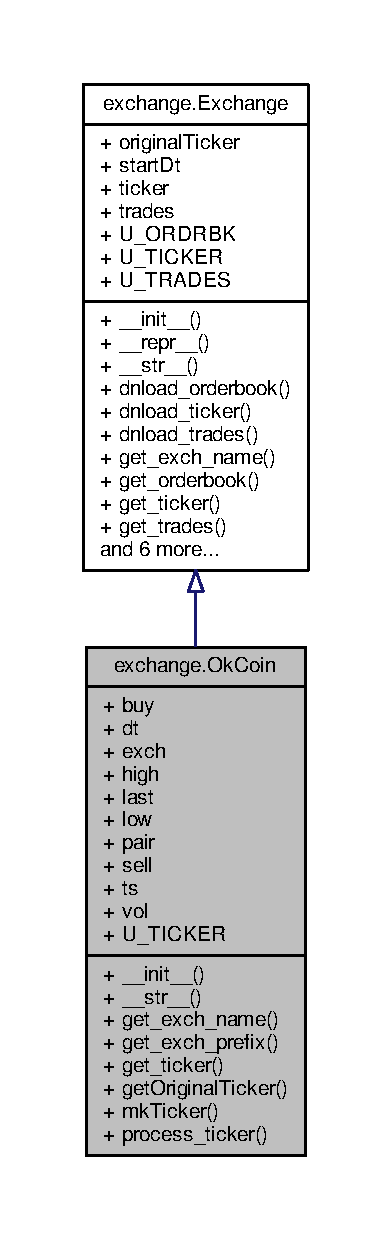
\includegraphics[height=550pt]{classexchange_1_1_ok_coin__inherit__graph}
\end{center}
\end{figure}


Collaboration diagram for exchange.\+Ok\+Coin\+:
\nopagebreak
\begin{figure}[H]
\begin{center}
\leavevmode
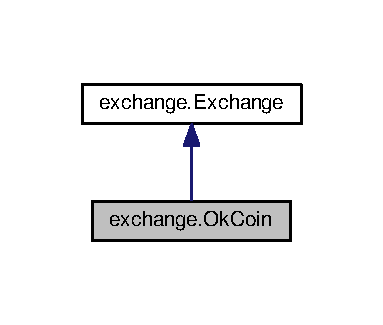
\includegraphics[height=550pt]{classexchange_1_1_ok_coin__coll__graph}
\end{center}
\end{figure}
\subsection*{Public Member Functions}
\begin{DoxyCompactItemize}
\item 
def \hyperlink{classexchange_1_1_ok_coin_ad3023a05231b37239fc5e2b220e2ae4c}{\+\_\+\+\_\+init\+\_\+\+\_\+} (self)
\item 
def \hyperlink{classexchange_1_1_ok_coin_af726894627f12bc46d199de5f454f2f4}{\+\_\+\+\_\+str\+\_\+\+\_\+} (self)
\item 
def \hyperlink{classexchange_1_1_ok_coin_a4bf45f3a1e9711ae38fd2eb01965e1d0}{get\+\_\+exch\+\_\+name} (self)
\item 
def \hyperlink{classexchange_1_1_ok_coin_a0ea57ae94a5e07e9387f830c67ceeed1}{get\+\_\+exch\+\_\+prefix} (self)
\item 
def \hyperlink{classexchange_1_1_ok_coin_a35425d16f4e0eb64677e32443fb4d91c}{get\+\_\+ticker} (self)
\item 
def \hyperlink{classexchange_1_1_ok_coin_aa3fa76e1280f612c3d0f7903d8847684}{get\+Original\+Ticker} (self)
\item 
def \hyperlink{classexchange_1_1_ok_coin_a7d835eb9a0e9603c5b540035c9caaa6a}{mk\+Ticker} (self)
\item 
def \hyperlink{classexchange_1_1_ok_coin_ac3ae7a770ea55b1b52ff0d909182d387}{process\+\_\+ticker} (self)
\end{DoxyCompactItemize}
\subsection*{Public Attributes}
\begin{DoxyCompactItemize}
\item 
\hyperlink{classexchange_1_1_ok_coin_aaf828e37142a83cbfb12d193313f6d43}{buy}
\item 
\hyperlink{classexchange_1_1_ok_coin_ade9d7cddcfa54f2b1ba5452854bfd48b}{dt}
\item 
\hyperlink{classexchange_1_1_ok_coin_a22678c192b53ddf34e8a636e0cdaf4d4}{exch}
\item 
\hyperlink{classexchange_1_1_ok_coin_af9d9dbcfc86404510e7f9a5704e8eecd}{high}
\item 
\hyperlink{classexchange_1_1_ok_coin_a726afbe3a75835fdcbe523aed8d6763c}{last}
\item 
\hyperlink{classexchange_1_1_ok_coin_a1afa53e0ad63830d0585288abea42094}{low}
\item 
\hyperlink{classexchange_1_1_ok_coin_a52f3b919f86565518d46c49c5b8f66a6}{pair}
\item 
\hyperlink{classexchange_1_1_ok_coin_aadb487d2e2f277374a747e1bcb0bd40b}{sell}
\item 
\hyperlink{classexchange_1_1_ok_coin_a0fe6263a7f58a6fa8a688929976b7e4a}{ts}
\item 
\hyperlink{classexchange_1_1_ok_coin_ad0e78d6b3c0a24504be72a0216fc6549}{vol}
\end{DoxyCompactItemize}
\subsection*{Static Public Attributes}
\begin{DoxyCompactItemize}
\item 
string \hyperlink{classexchange_1_1_ok_coin_a81305ced2eb23b94feb7195d1d42afc2}{U\+\_\+\+T\+I\+C\+K\+ER} = \textquotesingle{}https\+://www.\+okcoin.\+com/api/v1/ticker.\+do?symbol=btc\+\_\+usd\textquotesingle{}
\end{DoxyCompactItemize}


\subsection{Detailed Description}


Definition at line \hyperlink{exchange_8py_source_l00697}{697} of file \hyperlink{exchange_8py_source}{exchange.\+py}.



\subsection{Constructor \& Destructor Documentation}
\mbox{\Hypertarget{classexchange_1_1_ok_coin_ad3023a05231b37239fc5e2b220e2ae4c}\label{classexchange_1_1_ok_coin_ad3023a05231b37239fc5e2b220e2ae4c}} 
\index{exchange\+::\+Ok\+Coin@{exchange\+::\+Ok\+Coin}!\+\_\+\+\_\+init\+\_\+\+\_\+@{\+\_\+\+\_\+init\+\_\+\+\_\+}}
\index{\+\_\+\+\_\+init\+\_\+\+\_\+@{\+\_\+\+\_\+init\+\_\+\+\_\+}!exchange\+::\+Ok\+Coin@{exchange\+::\+Ok\+Coin}}
\subsubsection{\texorpdfstring{\+\_\+\+\_\+init\+\_\+\+\_\+()}{\_\_init\_\_()}}
{\footnotesize\ttfamily def exchange.\+Ok\+Coin.\+\_\+\+\_\+init\+\_\+\+\_\+ (\begin{DoxyParamCaption}\item[{}]{self }\end{DoxyParamCaption})}



Definition at line \hyperlink{exchange_8py_source_l00700}{700} of file \hyperlink{exchange_8py_source}{exchange.\+py}.


\begin{DoxyCode}
00700     \textcolor{keyword}{def }\hyperlink{namespacestart__time_a9c9bd378729a13c96a22c8b079ea172c}{\_\_init\_\_} (self):
00701         super ().\_\_init\_\_ ()
00702         
\end{DoxyCode}


\subsection{Member Function Documentation}
\mbox{\Hypertarget{classexchange_1_1_ok_coin_af726894627f12bc46d199de5f454f2f4}\label{classexchange_1_1_ok_coin_af726894627f12bc46d199de5f454f2f4}} 
\index{exchange\+::\+Ok\+Coin@{exchange\+::\+Ok\+Coin}!\+\_\+\+\_\+str\+\_\+\+\_\+@{\+\_\+\+\_\+str\+\_\+\+\_\+}}
\index{\+\_\+\+\_\+str\+\_\+\+\_\+@{\+\_\+\+\_\+str\+\_\+\+\_\+}!exchange\+::\+Ok\+Coin@{exchange\+::\+Ok\+Coin}}
\subsubsection{\texorpdfstring{\+\_\+\+\_\+str\+\_\+\+\_\+()}{\_\_str\_\_()}}
{\footnotesize\ttfamily def exchange.\+Ok\+Coin.\+\_\+\+\_\+str\+\_\+\+\_\+ (\begin{DoxyParamCaption}\item[{}]{self }\end{DoxyParamCaption})}



Definition at line \hyperlink{exchange_8py_source_l00756}{756} of file \hyperlink{exchange_8py_source}{exchange.\+py}.


\begin{DoxyCode}
00756     \textcolor{keyword}{def }\hyperlink{namespacerates_a2f1a70c33ee9e255938e4c19fd207264}{\_\_str\_\_} (self):
00757         result = json.dumps (self.\_\_dict\_\_, cls = DatetimeEncoder)
00758         
00759         \textcolor{comment}{# Normal function termination}
00760         \textcolor{keywordflow}{return} result
00761 
\end{DoxyCode}
\mbox{\Hypertarget{classexchange_1_1_ok_coin_a4bf45f3a1e9711ae38fd2eb01965e1d0}\label{classexchange_1_1_ok_coin_a4bf45f3a1e9711ae38fd2eb01965e1d0}} 
\index{exchange\+::\+Ok\+Coin@{exchange\+::\+Ok\+Coin}!get\+\_\+exch\+\_\+name@{get\+\_\+exch\+\_\+name}}
\index{get\+\_\+exch\+\_\+name@{get\+\_\+exch\+\_\+name}!exchange\+::\+Ok\+Coin@{exchange\+::\+Ok\+Coin}}
\subsubsection{\texorpdfstring{get\+\_\+exch\+\_\+name()}{get\_exch\_name()}}
{\footnotesize\ttfamily def exchange.\+Ok\+Coin.\+get\+\_\+exch\+\_\+name (\begin{DoxyParamCaption}\item[{}]{self }\end{DoxyParamCaption})}



Definition at line \hyperlink{exchange_8py_source_l00750}{750} of file \hyperlink{exchange_8py_source}{exchange.\+py}.


\begin{DoxyCode}
00750     \textcolor{keyword}{def }get\_exch\_name (self):
00751         \textcolor{keywordflow}{return} \textcolor{stringliteral}{"OkCoin"}
00752     
\end{DoxyCode}
\mbox{\Hypertarget{classexchange_1_1_ok_coin_a0ea57ae94a5e07e9387f830c67ceeed1}\label{classexchange_1_1_ok_coin_a0ea57ae94a5e07e9387f830c67ceeed1}} 
\index{exchange\+::\+Ok\+Coin@{exchange\+::\+Ok\+Coin}!get\+\_\+exch\+\_\+prefix@{get\+\_\+exch\+\_\+prefix}}
\index{get\+\_\+exch\+\_\+prefix@{get\+\_\+exch\+\_\+prefix}!exchange\+::\+Ok\+Coin@{exchange\+::\+Ok\+Coin}}
\subsubsection{\texorpdfstring{get\+\_\+exch\+\_\+prefix()}{get\_exch\_prefix()}}
{\footnotesize\ttfamily def exchange.\+Ok\+Coin.\+get\+\_\+exch\+\_\+prefix (\begin{DoxyParamCaption}\item[{}]{self }\end{DoxyParamCaption})}



Definition at line \hyperlink{exchange_8py_source_l00753}{753} of file \hyperlink{exchange_8py_source}{exchange.\+py}.


\begin{DoxyCode}
00753     \textcolor{keyword}{def }get\_exch\_prefix (self):
00754         \textcolor{keywordflow}{return} \textcolor{stringliteral}{"okc"}
00755         
\end{DoxyCode}
\mbox{\Hypertarget{classexchange_1_1_ok_coin_a35425d16f4e0eb64677e32443fb4d91c}\label{classexchange_1_1_ok_coin_a35425d16f4e0eb64677e32443fb4d91c}} 
\index{exchange\+::\+Ok\+Coin@{exchange\+::\+Ok\+Coin}!get\+\_\+ticker@{get\+\_\+ticker}}
\index{get\+\_\+ticker@{get\+\_\+ticker}!exchange\+::\+Ok\+Coin@{exchange\+::\+Ok\+Coin}}
\subsubsection{\texorpdfstring{get\+\_\+ticker()}{get\_ticker()}}
{\footnotesize\ttfamily def exchange.\+Ok\+Coin.\+get\+\_\+ticker (\begin{DoxyParamCaption}\item[{}]{self }\end{DoxyParamCaption})}



Definition at line \hyperlink{exchange_8py_source_l00716}{716} of file \hyperlink{exchange_8py_source}{exchange.\+py}.



References \hyperlink{exch2exch_8py_source_l00059}{exch2exch.\+Xbt\+Prices.\+buy}, \hyperlink{exchange_8py_source_l00060}{exchange.\+Ticker.\+buy}, \hyperlink{exchange_8py_source_l00430}{exchange.\+Bitfinex.\+buy}, \hyperlink{exchange_8py_source_l00502}{exchange.\+Bitstamp.\+buy}, \hyperlink{exchange_8py_source_l00574}{exchange.\+Fox\+Bit.\+buy}, \hyperlink{exchange_8py_source_l00642}{exchange.\+Mercado\+Bitcoin.\+buy}, \hyperlink{exchange_8py_source_l00707}{exchange.\+Ok\+Coin.\+buy}, \hyperlink{exch2exch_8py_source_l00028}{exch2exch.\+Rates.\+dt}, \hyperlink{exch2exch_8py_source_l00057}{exch2exch.\+Xbt\+Prices.\+dt}, \hyperlink{exchange_8py_source_l00059}{exchange.\+Ticker.\+dt}, \hyperlink{exchange_8py_source_l00437}{exchange.\+Bitfinex.\+dt}, \hyperlink{exchange_8py_source_l00509}{exchange.\+Bitstamp.\+dt}, \hyperlink{exchange_8py_source_l00573}{exchange.\+Fox\+Bit.\+dt}, \hyperlink{exchange_8py_source_l00649}{exchange.\+Mercado\+Bitcoin.\+dt}, \hyperlink{exchange_8py_source_l00714}{exchange.\+Ok\+Coin.\+dt}, \hyperlink{exch2exch_8py_source_l00061}{exch2exch.\+Xbt\+Prices.\+high}, \hyperlink{exchange_8py_source_l00062}{exchange.\+Ticker.\+high}, \hyperlink{exchange_8py_source_l00432}{exchange.\+Bitfinex.\+high}, \hyperlink{exchange_8py_source_l00504}{exchange.\+Bitstamp.\+high}, \hyperlink{exchange_8py_source_l00576}{exchange.\+Fox\+Bit.\+high}, \hyperlink{exchange_8py_source_l00644}{exchange.\+Mercado\+Bitcoin.\+high}, \hyperlink{exchange_8py_source_l00709}{exchange.\+Ok\+Coin.\+high}, \hyperlink{exch2exch_8py_source_l00063}{exch2exch.\+Xbt\+Prices.\+last}, \hyperlink{exchange_8py_source_l00064}{exchange.\+Ticker.\+last}, \hyperlink{exchange_8py_source_l00434}{exchange.\+Bitfinex.\+last}, \hyperlink{exchange_8py_source_l00506}{exchange.\+Bitstamp.\+last}, \hyperlink{exchange_8py_source_l00578}{exchange.\+Fox\+Bit.\+last}, \hyperlink{exchange_8py_source_l00646}{exchange.\+Mercado\+Bitcoin.\+last}, \hyperlink{exchange_8py_source_l00711}{exchange.\+Ok\+Coin.\+last}, \hyperlink{exch2exch_8py_source_l00062}{exch2exch.\+Xbt\+Prices.\+low}, \hyperlink{exchange_8py_source_l00063}{exchange.\+Ticker.\+low}, \hyperlink{exchange_8py_source_l00433}{exchange.\+Bitfinex.\+low}, \hyperlink{exchange_8py_source_l00505}{exchange.\+Bitstamp.\+low}, \hyperlink{exchange_8py_source_l00577}{exchange.\+Fox\+Bit.\+low}, \hyperlink{exchange_8py_source_l00645}{exchange.\+Mercado\+Bitcoin.\+low}, \hyperlink{exchange_8py_source_l00710}{exchange.\+Ok\+Coin.\+low}, \hyperlink{exch2exch_8py_source_l00058}{exch2exch.\+Xbt\+Prices.\+sell}, \hyperlink{exchange_8py_source_l00061}{exchange.\+Ticker.\+sell}, \hyperlink{exchange_8py_source_l00431}{exchange.\+Bitfinex.\+sell}, \hyperlink{exchange_8py_source_l00503}{exchange.\+Bitstamp.\+sell}, \hyperlink{exchange_8py_source_l00575}{exchange.\+Fox\+Bit.\+sell}, \hyperlink{exchange_8py_source_l00643}{exchange.\+Mercado\+Bitcoin.\+sell}, and \hyperlink{exchange_8py_source_l00708}{exchange.\+Ok\+Coin.\+sell}.


\begin{DoxyCode}
00716     \textcolor{keyword}{def }get\_ticker (self):
00717         super ().get\_ticker ()
00718         
00719         dt   = self.dt
00720         buy  = self.buy
00721         sell = self.sell
00722         high = self.high
00723         low  = self.low
00724         last = self.last
00725         
00726         result = (dt, sell, buy, high, low, last)
00727         
00728         \textcolor{keywordflow}{return} result
00729     
\end{DoxyCode}
\mbox{\Hypertarget{classexchange_1_1_ok_coin_aa3fa76e1280f612c3d0f7903d8847684}\label{classexchange_1_1_ok_coin_aa3fa76e1280f612c3d0f7903d8847684}} 
\index{exchange\+::\+Ok\+Coin@{exchange\+::\+Ok\+Coin}!get\+Original\+Ticker@{get\+Original\+Ticker}}
\index{get\+Original\+Ticker@{get\+Original\+Ticker}!exchange\+::\+Ok\+Coin@{exchange\+::\+Ok\+Coin}}
\subsubsection{\texorpdfstring{get\+Original\+Ticker()}{getOriginalTicker()}}
{\footnotesize\ttfamily def exchange.\+Ok\+Coin.\+get\+Original\+Ticker (\begin{DoxyParamCaption}\item[{}]{self }\end{DoxyParamCaption})}



Definition at line \hyperlink{exchange_8py_source_l00747}{747} of file \hyperlink{exchange_8py_source}{exchange.\+py}.



References \hyperlink{exchange_8py_source_l00186}{exchange.\+Exchange.\+original\+Ticker}.


\begin{DoxyCode}
00747     \textcolor{keyword}{def }getOriginalTicker (self):
00748         \textcolor{keywordflow}{return} self.originalTicker
00749     
\end{DoxyCode}
\mbox{\Hypertarget{classexchange_1_1_ok_coin_a7d835eb9a0e9603c5b540035c9caaa6a}\label{classexchange_1_1_ok_coin_a7d835eb9a0e9603c5b540035c9caaa6a}} 
\index{exchange\+::\+Ok\+Coin@{exchange\+::\+Ok\+Coin}!mk\+Ticker@{mk\+Ticker}}
\index{mk\+Ticker@{mk\+Ticker}!exchange\+::\+Ok\+Coin@{exchange\+::\+Ok\+Coin}}
\subsubsection{\texorpdfstring{mk\+Ticker()}{mkTicker()}}
{\footnotesize\ttfamily def exchange.\+Ok\+Coin.\+mk\+Ticker (\begin{DoxyParamCaption}\item[{}]{self }\end{DoxyParamCaption})}



Definition at line \hyperlink{exchange_8py_source_l00730}{730} of file \hyperlink{exchange_8py_source}{exchange.\+py}.



References \hyperlink{exch2exch_8py_source_l00059}{exch2exch.\+Xbt\+Prices.\+buy}, \hyperlink{exchange_8py_source_l00060}{exchange.\+Ticker.\+buy}, \hyperlink{exchange_8py_source_l00430}{exchange.\+Bitfinex.\+buy}, \hyperlink{exchange_8py_source_l00502}{exchange.\+Bitstamp.\+buy}, \hyperlink{exchange_8py_source_l00574}{exchange.\+Fox\+Bit.\+buy}, \hyperlink{exchange_8py_source_l00642}{exchange.\+Mercado\+Bitcoin.\+buy}, \hyperlink{exchange_8py_source_l00707}{exchange.\+Ok\+Coin.\+buy}, \hyperlink{exchange_8py_source_l00057}{exchange.\+Ticker.\+exch}, \hyperlink{exch2exch_8py_source_l00064}{exch2exch.\+Xbt\+Prices.\+exch}, \hyperlink{exchange_8py_source_l00424}{exchange.\+Bitfinex.\+exch}, \hyperlink{exchange_8py_source_l00499}{exchange.\+Bitstamp.\+exch}, \hyperlink{exchange_8py_source_l00567}{exchange.\+Fox\+Bit.\+exch}, \hyperlink{exchange_8py_source_l00639}{exchange.\+Mercado\+Bitcoin.\+exch}, \hyperlink{exchange_8py_source_l00704}{exchange.\+Ok\+Coin.\+exch}, \hyperlink{exch2exch_8py_source_l00061}{exch2exch.\+Xbt\+Prices.\+high}, \hyperlink{exchange_8py_source_l00062}{exchange.\+Ticker.\+high}, \hyperlink{exchange_8py_source_l00432}{exchange.\+Bitfinex.\+high}, \hyperlink{exchange_8py_source_l00504}{exchange.\+Bitstamp.\+high}, \hyperlink{exchange_8py_source_l00576}{exchange.\+Fox\+Bit.\+high}, \hyperlink{exchange_8py_source_l00644}{exchange.\+Mercado\+Bitcoin.\+high}, \hyperlink{exchange_8py_source_l00709}{exchange.\+Ok\+Coin.\+high}, \hyperlink{exch2exch_8py_source_l00063}{exch2exch.\+Xbt\+Prices.\+last}, \hyperlink{exchange_8py_source_l00064}{exchange.\+Ticker.\+last}, \hyperlink{exchange_8py_source_l00434}{exchange.\+Bitfinex.\+last}, \hyperlink{exchange_8py_source_l00506}{exchange.\+Bitstamp.\+last}, \hyperlink{exchange_8py_source_l00578}{exchange.\+Fox\+Bit.\+last}, \hyperlink{exchange_8py_source_l00646}{exchange.\+Mercado\+Bitcoin.\+last}, \hyperlink{exchange_8py_source_l00711}{exchange.\+Ok\+Coin.\+last}, \hyperlink{exch2exch_8py_source_l00062}{exch2exch.\+Xbt\+Prices.\+low}, \hyperlink{exchange_8py_source_l00063}{exchange.\+Ticker.\+low}, \hyperlink{exchange_8py_source_l00433}{exchange.\+Bitfinex.\+low}, \hyperlink{exchange_8py_source_l00505}{exchange.\+Bitstamp.\+low}, \hyperlink{exchange_8py_source_l00577}{exchange.\+Fox\+Bit.\+low}, \hyperlink{exchange_8py_source_l00645}{exchange.\+Mercado\+Bitcoin.\+low}, \hyperlink{exchange_8py_source_l00710}{exchange.\+Ok\+Coin.\+low}, \hyperlink{exchange_8py_source_l00058}{exchange.\+Ticker.\+pair}, \hyperlink{exchange_8py_source_l00425}{exchange.\+Bitfinex.\+pair}, \hyperlink{exchange_8py_source_l00500}{exchange.\+Bitstamp.\+pair}, \hyperlink{exchange_8py_source_l00568}{exchange.\+Fox\+Bit.\+pair}, \hyperlink{exchange_8py_source_l00640}{exchange.\+Mercado\+Bitcoin.\+pair}, \hyperlink{exchange_8py_source_l00705}{exchange.\+Ok\+Coin.\+pair}, \hyperlink{exch2exch_8py_source_l00058}{exch2exch.\+Xbt\+Prices.\+sell}, \hyperlink{exchange_8py_source_l00061}{exchange.\+Ticker.\+sell}, \hyperlink{exchange_8py_source_l00431}{exchange.\+Bitfinex.\+sell}, \hyperlink{exchange_8py_source_l00503}{exchange.\+Bitstamp.\+sell}, \hyperlink{exchange_8py_source_l00575}{exchange.\+Fox\+Bit.\+sell}, \hyperlink{exchange_8py_source_l00643}{exchange.\+Mercado\+Bitcoin.\+sell}, \hyperlink{exchange_8py_source_l00708}{exchange.\+Ok\+Coin.\+sell}, \hyperlink{exchange_8py_source_l00428}{exchange.\+Bitfinex.\+ts}, \hyperlink{exchange_8py_source_l00501}{exchange.\+Bitstamp.\+ts}, \hyperlink{exchange_8py_source_l00641}{exchange.\+Mercado\+Bitcoin.\+ts}, \hyperlink{exchange_8py_source_l00706}{exchange.\+Ok\+Coin.\+ts}, \hyperlink{exchange_8py_source_l00065}{exchange.\+Ticker.\+vol}, \hyperlink{exchange_8py_source_l00435}{exchange.\+Bitfinex.\+vol}, \hyperlink{exchange_8py_source_l00507}{exchange.\+Bitstamp.\+vol}, \hyperlink{exchange_8py_source_l00647}{exchange.\+Mercado\+Bitcoin.\+vol}, and \hyperlink{exchange_8py_source_l00712}{exchange.\+Ok\+Coin.\+vol}.


\begin{DoxyCode}
00730     \textcolor{keyword}{def }mkTicker (self):
00731         super ().get\_ticker ()
00732         
00733         exch = self.exch
00734         pair = self.pair
00735         dt   = self.ts
00736         buy  = self.buy
00737         sell = self.sell
00738         high = self.high
00739         low  = self.low
00740         last = self.last
00741         vol  = self.vol
00742         
00743         result = Ticker (exch, pair, dt, buy, sell, high, low, last, vol)
00744         
00745         \textcolor{keywordflow}{return} result
00746         
\end{DoxyCode}
\mbox{\Hypertarget{classexchange_1_1_ok_coin_ac3ae7a770ea55b1b52ff0d909182d387}\label{classexchange_1_1_ok_coin_ac3ae7a770ea55b1b52ff0d909182d387}} 
\index{exchange\+::\+Ok\+Coin@{exchange\+::\+Ok\+Coin}!process\+\_\+ticker@{process\+\_\+ticker}}
\index{process\+\_\+ticker@{process\+\_\+ticker}!exchange\+::\+Ok\+Coin@{exchange\+::\+Ok\+Coin}}
\subsubsection{\texorpdfstring{process\+\_\+ticker()}{process\_ticker()}}
{\footnotesize\ttfamily def exchange.\+Ok\+Coin.\+process\+\_\+ticker (\begin{DoxyParamCaption}\item[{}]{self }\end{DoxyParamCaption})}



Definition at line \hyperlink{exchange_8py_source_l00703}{703} of file \hyperlink{exchange_8py_source}{exchange.\+py}.


\begin{DoxyCode}
00703     \textcolor{keyword}{def }process\_ticker (self):
00704         self.exch = self.get\_exch\_name ()
00705         self.pair = \textcolor{stringliteral}{'BTCUSD'}
00706         self.ts   = int   (self.ticker[\textcolor{stringliteral}{'date'}])
00707         self.buy  = float (self.ticker[\textcolor{stringliteral}{'ticker'}][\textcolor{stringliteral}{'buy'}])
00708         self.sell = float (self.ticker[\textcolor{stringliteral}{'ticker'}][\textcolor{stringliteral}{'sell'}])
00709         self.high = float (self.ticker[\textcolor{stringliteral}{'ticker'}][\textcolor{stringliteral}{'high'}])
00710         self.low  = float (self.ticker[\textcolor{stringliteral}{'ticker'}][\textcolor{stringliteral}{'low'}])
00711         self.last = float (self.ticker[\textcolor{stringliteral}{'ticker'}][\textcolor{stringliteral}{'last'}])
00712         self.vol  = float (self.ticker[\textcolor{stringliteral}{'ticker'}][\textcolor{stringliteral}{'vol'}])
00713     
00714         self.dt = datetime.datetime.fromtimestamp (float (self.ts))
00715     
\end{DoxyCode}


\subsection{Member Data Documentation}
\mbox{\Hypertarget{classexchange_1_1_ok_coin_aaf828e37142a83cbfb12d193313f6d43}\label{classexchange_1_1_ok_coin_aaf828e37142a83cbfb12d193313f6d43}} 
\index{exchange\+::\+Ok\+Coin@{exchange\+::\+Ok\+Coin}!buy@{buy}}
\index{buy@{buy}!exchange\+::\+Ok\+Coin@{exchange\+::\+Ok\+Coin}}
\subsubsection{\texorpdfstring{buy}{buy}}
{\footnotesize\ttfamily exchange.\+Ok\+Coin.\+buy}



Definition at line \hyperlink{exchange_8py_source_l00707}{707} of file \hyperlink{exchange_8py_source}{exchange.\+py}.



Referenced by \hyperlink{raw__urlparser_8py_source_l00074}{raw\+\_\+urlparser.\+Xbt\+Prices.\+\_\+\+\_\+str\+\_\+\+\_\+()}, \hyperlink{exchange_8py_source_l00716}{exchange.\+Ok\+Coin.\+get\+\_\+ticker()}, \hyperlink{raw__urlparser_8py_source_l00062}{raw\+\_\+urlparser.\+Xbt\+Prices.\+get\+Buy()}, and \hyperlink{exchange_8py_source_l00730}{exchange.\+Ok\+Coin.\+mk\+Ticker()}.

\mbox{\Hypertarget{classexchange_1_1_ok_coin_ade9d7cddcfa54f2b1ba5452854bfd48b}\label{classexchange_1_1_ok_coin_ade9d7cddcfa54f2b1ba5452854bfd48b}} 
\index{exchange\+::\+Ok\+Coin@{exchange\+::\+Ok\+Coin}!dt@{dt}}
\index{dt@{dt}!exchange\+::\+Ok\+Coin@{exchange\+::\+Ok\+Coin}}
\subsubsection{\texorpdfstring{dt}{dt}}
{\footnotesize\ttfamily exchange.\+Ok\+Coin.\+dt}



Definition at line \hyperlink{exchange_8py_source_l00714}{714} of file \hyperlink{exchange_8py_source}{exchange.\+py}.



Referenced by \hyperlink{start__time_2____init_____8py_source_l00034}{start\+\_\+time.\+Date\+Time.\+\_\+\+\_\+str\+\_\+\+\_\+()}, \hyperlink{raw__urlparser_8py_source_l00038}{raw\+\_\+urlparser.\+Rates.\+\_\+\+\_\+str\+\_\+\+\_\+()}, \hyperlink{raw__urlparser_8py_source_l00074}{raw\+\_\+urlparser.\+Xbt\+Prices.\+\_\+\+\_\+str\+\_\+\+\_\+()}, \hyperlink{exchange_8py_source_l00716}{exchange.\+Ok\+Coin.\+get\+\_\+ticker()}, \hyperlink{start__time_2____init_____8py_source_l00031}{start\+\_\+time.\+Date\+Time.\+get\+Datetime()}, and \hyperlink{raw__urlparser_8py_source_l00059}{raw\+\_\+urlparser.\+Xbt\+Prices.\+get\+Date\+Time()}.

\mbox{\Hypertarget{classexchange_1_1_ok_coin_a22678c192b53ddf34e8a636e0cdaf4d4}\label{classexchange_1_1_ok_coin_a22678c192b53ddf34e8a636e0cdaf4d4}} 
\index{exchange\+::\+Ok\+Coin@{exchange\+::\+Ok\+Coin}!exch@{exch}}
\index{exch@{exch}!exchange\+::\+Ok\+Coin@{exchange\+::\+Ok\+Coin}}
\subsubsection{\texorpdfstring{exch}{exch}}
{\footnotesize\ttfamily exchange.\+Ok\+Coin.\+exch}



Definition at line \hyperlink{exchange_8py_source_l00704}{704} of file \hyperlink{exchange_8py_source}{exchange.\+py}.



Referenced by \hyperlink{raw__urlparser_8py_source_l00074}{raw\+\_\+urlparser.\+Xbt\+Prices.\+\_\+\+\_\+str\+\_\+\+\_\+()}, \hyperlink{raw__urlparser_8py_source_l00068}{raw\+\_\+urlparser.\+Xbt\+Prices.\+get\+Exchange\+Name()}, and \hyperlink{exchange_8py_source_l00730}{exchange.\+Ok\+Coin.\+mk\+Ticker()}.

\mbox{\Hypertarget{classexchange_1_1_ok_coin_af9d9dbcfc86404510e7f9a5704e8eecd}\label{classexchange_1_1_ok_coin_af9d9dbcfc86404510e7f9a5704e8eecd}} 
\index{exchange\+::\+Ok\+Coin@{exchange\+::\+Ok\+Coin}!high@{high}}
\index{high@{high}!exchange\+::\+Ok\+Coin@{exchange\+::\+Ok\+Coin}}
\subsubsection{\texorpdfstring{high}{high}}
{\footnotesize\ttfamily exchange.\+Ok\+Coin.\+high}



Definition at line \hyperlink{exchange_8py_source_l00709}{709} of file \hyperlink{exchange_8py_source}{exchange.\+py}.



Referenced by \hyperlink{exchange_8py_source_l00716}{exchange.\+Ok\+Coin.\+get\+\_\+ticker()}, and \hyperlink{exchange_8py_source_l00730}{exchange.\+Ok\+Coin.\+mk\+Ticker()}.

\mbox{\Hypertarget{classexchange_1_1_ok_coin_a726afbe3a75835fdcbe523aed8d6763c}\label{classexchange_1_1_ok_coin_a726afbe3a75835fdcbe523aed8d6763c}} 
\index{exchange\+::\+Ok\+Coin@{exchange\+::\+Ok\+Coin}!last@{last}}
\index{last@{last}!exchange\+::\+Ok\+Coin@{exchange\+::\+Ok\+Coin}}
\subsubsection{\texorpdfstring{last}{last}}
{\footnotesize\ttfamily exchange.\+Ok\+Coin.\+last}



Definition at line \hyperlink{exchange_8py_source_l00711}{711} of file \hyperlink{exchange_8py_source}{exchange.\+py}.



Referenced by \hyperlink{exchange_8py_source_l00716}{exchange.\+Ok\+Coin.\+get\+\_\+ticker()}, and \hyperlink{exchange_8py_source_l00730}{exchange.\+Ok\+Coin.\+mk\+Ticker()}.

\mbox{\Hypertarget{classexchange_1_1_ok_coin_a1afa53e0ad63830d0585288abea42094}\label{classexchange_1_1_ok_coin_a1afa53e0ad63830d0585288abea42094}} 
\index{exchange\+::\+Ok\+Coin@{exchange\+::\+Ok\+Coin}!low@{low}}
\index{low@{low}!exchange\+::\+Ok\+Coin@{exchange\+::\+Ok\+Coin}}
\subsubsection{\texorpdfstring{low}{low}}
{\footnotesize\ttfamily exchange.\+Ok\+Coin.\+low}



Definition at line \hyperlink{exchange_8py_source_l00710}{710} of file \hyperlink{exchange_8py_source}{exchange.\+py}.



Referenced by \hyperlink{exchange_8py_source_l00716}{exchange.\+Ok\+Coin.\+get\+\_\+ticker()}, and \hyperlink{exchange_8py_source_l00730}{exchange.\+Ok\+Coin.\+mk\+Ticker()}.

\mbox{\Hypertarget{classexchange_1_1_ok_coin_a52f3b919f86565518d46c49c5b8f66a6}\label{classexchange_1_1_ok_coin_a52f3b919f86565518d46c49c5b8f66a6}} 
\index{exchange\+::\+Ok\+Coin@{exchange\+::\+Ok\+Coin}!pair@{pair}}
\index{pair@{pair}!exchange\+::\+Ok\+Coin@{exchange\+::\+Ok\+Coin}}
\subsubsection{\texorpdfstring{pair}{pair}}
{\footnotesize\ttfamily exchange.\+Ok\+Coin.\+pair}



Definition at line \hyperlink{exchange_8py_source_l00705}{705} of file \hyperlink{exchange_8py_source}{exchange.\+py}.



Referenced by \hyperlink{exchange_8py_source_l00730}{exchange.\+Ok\+Coin.\+mk\+Ticker()}.

\mbox{\Hypertarget{classexchange_1_1_ok_coin_aadb487d2e2f277374a747e1bcb0bd40b}\label{classexchange_1_1_ok_coin_aadb487d2e2f277374a747e1bcb0bd40b}} 
\index{exchange\+::\+Ok\+Coin@{exchange\+::\+Ok\+Coin}!sell@{sell}}
\index{sell@{sell}!exchange\+::\+Ok\+Coin@{exchange\+::\+Ok\+Coin}}
\subsubsection{\texorpdfstring{sell}{sell}}
{\footnotesize\ttfamily exchange.\+Ok\+Coin.\+sell}



Definition at line \hyperlink{exchange_8py_source_l00708}{708} of file \hyperlink{exchange_8py_source}{exchange.\+py}.



Referenced by \hyperlink{raw__urlparser_8py_source_l00074}{raw\+\_\+urlparser.\+Xbt\+Prices.\+\_\+\+\_\+str\+\_\+\+\_\+()}, \hyperlink{exchange_8py_source_l00716}{exchange.\+Ok\+Coin.\+get\+\_\+ticker()}, \hyperlink{raw__urlparser_8py_source_l00065}{raw\+\_\+urlparser.\+Xbt\+Prices.\+get\+Sell()}, and \hyperlink{exchange_8py_source_l00730}{exchange.\+Ok\+Coin.\+mk\+Ticker()}.

\mbox{\Hypertarget{classexchange_1_1_ok_coin_a0fe6263a7f58a6fa8a688929976b7e4a}\label{classexchange_1_1_ok_coin_a0fe6263a7f58a6fa8a688929976b7e4a}} 
\index{exchange\+::\+Ok\+Coin@{exchange\+::\+Ok\+Coin}!ts@{ts}}
\index{ts@{ts}!exchange\+::\+Ok\+Coin@{exchange\+::\+Ok\+Coin}}
\subsubsection{\texorpdfstring{ts}{ts}}
{\footnotesize\ttfamily exchange.\+Ok\+Coin.\+ts}



Definition at line \hyperlink{exchange_8py_source_l00706}{706} of file \hyperlink{exchange_8py_source}{exchange.\+py}.



Referenced by \hyperlink{exchange_8py_source_l00730}{exchange.\+Ok\+Coin.\+mk\+Ticker()}.

\mbox{\Hypertarget{classexchange_1_1_ok_coin_a81305ced2eb23b94feb7195d1d42afc2}\label{classexchange_1_1_ok_coin_a81305ced2eb23b94feb7195d1d42afc2}} 
\index{exchange\+::\+Ok\+Coin@{exchange\+::\+Ok\+Coin}!U\+\_\+\+T\+I\+C\+K\+ER@{U\+\_\+\+T\+I\+C\+K\+ER}}
\index{U\+\_\+\+T\+I\+C\+K\+ER@{U\+\_\+\+T\+I\+C\+K\+ER}!exchange\+::\+Ok\+Coin@{exchange\+::\+Ok\+Coin}}
\subsubsection{\texorpdfstring{U\+\_\+\+T\+I\+C\+K\+ER}{U\_TICKER}}
{\footnotesize\ttfamily string exchange.\+Ok\+Coin.\+U\+\_\+\+T\+I\+C\+K\+ER = \textquotesingle{}https\+://www.\+okcoin.\+com/api/v1/ticker.\+do?symbol=btc\+\_\+usd\textquotesingle{}\hspace{0.3cm}{\ttfamily [static]}}



Definition at line \hyperlink{exchange_8py_source_l00698}{698} of file \hyperlink{exchange_8py_source}{exchange.\+py}.

\mbox{\Hypertarget{classexchange_1_1_ok_coin_ad0e78d6b3c0a24504be72a0216fc6549}\label{classexchange_1_1_ok_coin_ad0e78d6b3c0a24504be72a0216fc6549}} 
\index{exchange\+::\+Ok\+Coin@{exchange\+::\+Ok\+Coin}!vol@{vol}}
\index{vol@{vol}!exchange\+::\+Ok\+Coin@{exchange\+::\+Ok\+Coin}}
\subsubsection{\texorpdfstring{vol}{vol}}
{\footnotesize\ttfamily exchange.\+Ok\+Coin.\+vol}



Definition at line \hyperlink{exchange_8py_source_l00712}{712} of file \hyperlink{exchange_8py_source}{exchange.\+py}.



Referenced by \hyperlink{exchange_8py_source_l00730}{exchange.\+Ok\+Coin.\+mk\+Ticker()}.



The documentation for this class was generated from the following file\+:\begin{DoxyCompactItemize}
\item 
/home/hilton/github/exch2exh/\hyperlink{exchange_8py}{exchange.\+py}\end{DoxyCompactItemize}

\hypertarget{classexchange_1_1_order_book}{}\section{exchange.\+Order\+Book Class Reference}
\label{classexchange_1_1_order_book}\index{exchange.\+Order\+Book@{exchange.\+Order\+Book}}


Collaboration diagram for exchange.\+Order\+Book\+:\nopagebreak
\begin{figure}[H]
\begin{center}
\leavevmode
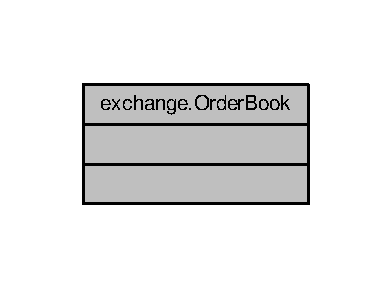
\includegraphics[width=188pt]{classexchange_1_1_order_book__coll__graph}
\end{center}
\end{figure}


\subsection{Detailed Description}


Definition at line \hyperlink{exchange_8py_source_l00038}{38} of file \hyperlink{exchange_8py_source}{exchange.\+py}.



The documentation for this class was generated from the following file\+:\begin{DoxyCompactItemize}
\item 
/home/hilton/github/exch2exh/\hyperlink{exchange_8py}{exchange.\+py}\end{DoxyCompactItemize}

\hypertarget{classe2e_1_1_parameters}{}\section{e2e.\+Parameters Class Reference}
\label{classe2e_1_1_parameters}\index{e2e.\+Parameters@{e2e.\+Parameters}}


Collaboration diagram for e2e.\+Parameters\+:\nopagebreak
\begin{figure}[H]
\begin{center}
\leavevmode
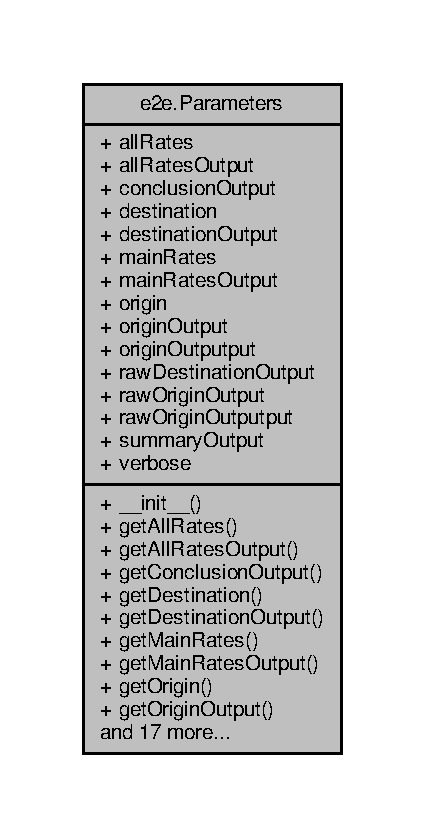
\includegraphics[width=204pt]{classe2e_1_1_parameters__coll__graph}
\end{center}
\end{figure}
\subsection*{Public Member Functions}
\begin{DoxyCompactItemize}
\item 
def \hyperlink{classe2e_1_1_parameters_a335faddfa9af3ed8ac441e92faec0946}{\+\_\+\+\_\+init\+\_\+\+\_\+} (self)
\item 
def \hyperlink{classe2e_1_1_parameters_a2eb01ddbfa9f2b75f8d901196e260a52}{get\+Alt\+Rate} (self)
\item 
def \hyperlink{classe2e_1_1_parameters_acc3f1ce2de05c433834b52689c50cef6}{get\+Alt\+Rate\+Output} (self)
\item 
def \hyperlink{classe2e_1_1_parameters_ac4ff6b23493a25723cfe99fb7becf328}{get\+Conclusion\+Output} (self)
\item 
def \hyperlink{classe2e_1_1_parameters_ad984826a5973fff569b554b44245b714}{get\+Destination} (self)
\item 
def \hyperlink{classe2e_1_1_parameters_a4451a6d8224c2216fdef8e53e55fadaf}{get\+Destination\+Output} (self)
\item 
def \hyperlink{classe2e_1_1_parameters_a152d1d8c15164a06b54c3339bc9d15bf}{get\+Main\+Rate} (self)
\item 
def \hyperlink{classe2e_1_1_parameters_ae4d5b651e4e6434f0779f4661c163166}{get\+Main\+Rate\+Output} (self)
\item 
def \hyperlink{classe2e_1_1_parameters_ac570cc2f199bcb82a4634be79110a013}{get\+Origin} (self)
\item 
def \hyperlink{classe2e_1_1_parameters_af0cdd8e6726ccc72387e466c2abe04c2}{get\+Origin\+Output} (self)
\item 
def \hyperlink{classe2e_1_1_parameters_a0536c6870c6371025927f435e47704ed}{get\+Raw\+Destination\+Output} (self)
\item 
def \hyperlink{classe2e_1_1_parameters_a4ed96c7861e649d101984ff5c8056691}{get\+Raw\+Origin\+Output} (self)
\item 
def \hyperlink{classe2e_1_1_parameters_a46f3f35e99d7ce8a22fa34d66a348586}{get\+Summary\+Output} (self)
\item 
def \hyperlink{classe2e_1_1_parameters_a1e5e7e1986b641b01d4c24690a6d48eb}{get\+Verbose} (self)
\item 
def \hyperlink{classe2e_1_1_parameters_a1e73f515a94469c6b9c75a595d8ae426}{set\+Alt\+Rate} (self, \hyperlink{classe2e_1_1_parameters_a9d12e65d35b0807822c8774101ff613d}{alt\+Rate})
\item 
def \hyperlink{classe2e_1_1_parameters_a47d3280dcce660c7227ca8c817859d84}{set\+Alt\+Rate\+Output} (self, \hyperlink{classe2e_1_1_parameters_ab0fc4de0f4d6d135eea22cae77536807}{alt\+Rate\+Output})
\item 
def \hyperlink{classe2e_1_1_parameters_a4ec249739947f4643b6d2dc811ef2639}{set\+Conclusion\+Output} (self, \hyperlink{classe2e_1_1_parameters_ad5967b78ebf5c8778e423413053015a7}{conclusion\+Output})
\item 
def \hyperlink{classe2e_1_1_parameters_ac63ae6d2b5f45ae78ee855953a038f14}{set\+Destination} (self, \hyperlink{classe2e_1_1_parameters_ad2cdf746b8890c53a9cab6fd7df7043b}{destination})
\item 
def \hyperlink{classe2e_1_1_parameters_a96083de53012ca50d2a345a1673802de}{set\+Destination\+Output} (self, \hyperlink{classe2e_1_1_parameters_a3b4ae5aa9b73466e51018b6f37792577}{destination\+Output})
\item 
def \hyperlink{classe2e_1_1_parameters_a8cea2f8656650dfbc2f4b9c13bce46a4}{set\+Main\+Rate} (self, \hyperlink{classe2e_1_1_parameters_a3d473f94dbb62a1488945cf6abc9f108}{main\+Rate})
\item 
def \hyperlink{classe2e_1_1_parameters_a930e9e6cafab4096286754a473617232}{set\+Main\+Rate\+Output} (self, \hyperlink{classe2e_1_1_parameters_acff858a94aecf1e5a553273e8acd9eca}{main\+Rate\+Output})
\item 
def \hyperlink{classe2e_1_1_parameters_a421e56e53ff0aaf5222229d8a81c456b}{set\+Origin} (self, \hyperlink{classe2e_1_1_parameters_aff4d7aaa35295f7f71e546fe5554c4d9}{origin})
\item 
def \hyperlink{classe2e_1_1_parameters_a2b87a3357a16d35b7606a97e924a4904}{set\+Origin\+Output} (self, \hyperlink{classe2e_1_1_parameters_ab1ac2fc0ab2f3ef169b776c776cdb225}{origin\+Output})
\item 
def \hyperlink{classe2e_1_1_parameters_a2a4420c79bef43533fe2d9562d0faedb}{set\+Raw\+Destination\+Output} (self, \hyperlink{classe2e_1_1_parameters_a84b319098084ed505e089a600e154f6e}{raw\+Destination\+Output})
\item 
def \hyperlink{classe2e_1_1_parameters_a6a69b8936b79b34f612b3dda7bedc67f}{set\+Raw\+Origin\+Output} (self, \hyperlink{classe2e_1_1_parameters_a62b586d9863422872833e34814ac51e6}{raw\+Origin\+Output})
\item 
def \hyperlink{classe2e_1_1_parameters_af904cdd913f0ffd64f28c9f7b1137389}{set\+Summary\+Output} (self, \hyperlink{classe2e_1_1_parameters_a1f4bab2e746d2c598e20ccba0154d795}{summary\+Output})
\item 
def \hyperlink{classe2e_1_1_parameters_a9d1ef6cf9aaac08105966db43687423f}{set\+Verbose} (self, \hyperlink{classe2e_1_1_parameters_a84d862bf507bb0325f5daf3b7e5d9ab3}{verbose})
\end{DoxyCompactItemize}
\subsection*{Public Attributes}
\begin{DoxyCompactItemize}
\item 
\hyperlink{classe2e_1_1_parameters_a9d12e65d35b0807822c8774101ff613d}{alt\+Rate}
\item 
\hyperlink{classe2e_1_1_parameters_ab0fc4de0f4d6d135eea22cae77536807}{alt\+Rate\+Output}
\item 
\hyperlink{classe2e_1_1_parameters_a7f2806bfda6a689e9140610da6812dce}{alt\+Rates}
\item 
\hyperlink{classe2e_1_1_parameters_a30566bb6c78f0f438e993696b9fa9f20}{alt\+Rates\+Output}
\item 
\hyperlink{classe2e_1_1_parameters_ad5967b78ebf5c8778e423413053015a7}{conclusion\+Output}
\item 
\hyperlink{classe2e_1_1_parameters_ad2cdf746b8890c53a9cab6fd7df7043b}{destination}
\item 
\hyperlink{classe2e_1_1_parameters_a3b4ae5aa9b73466e51018b6f37792577}{destination\+Output}
\item 
\hyperlink{classe2e_1_1_parameters_a3d473f94dbb62a1488945cf6abc9f108}{main\+Rate}
\item 
\hyperlink{classe2e_1_1_parameters_acff858a94aecf1e5a553273e8acd9eca}{main\+Rate\+Output}
\item 
\hyperlink{classe2e_1_1_parameters_aaa2b41d7017ab4893bbe27fa8edb7180}{main\+Rates}
\item 
\hyperlink{classe2e_1_1_parameters_a552470d8541b7caf2bb8940e32a6fe0e}{main\+Rates\+Output}
\item 
\hyperlink{classe2e_1_1_parameters_aff4d7aaa35295f7f71e546fe5554c4d9}{origin}
\item 
\hyperlink{classe2e_1_1_parameters_ab1ac2fc0ab2f3ef169b776c776cdb225}{origin\+Output}
\item 
\hyperlink{classe2e_1_1_parameters_acece0ee5caaa6322c3a337c3b7f00599}{origin\+Outputput}
\item 
\hyperlink{classe2e_1_1_parameters_a84b319098084ed505e089a600e154f6e}{raw\+Destination\+Output}
\item 
\hyperlink{classe2e_1_1_parameters_a62b586d9863422872833e34814ac51e6}{raw\+Origin\+Output}
\item 
\hyperlink{classe2e_1_1_parameters_a363d9432d8f2bdcf645fa39b81e007f3}{raw\+Origin\+Outputput}
\item 
\hyperlink{classe2e_1_1_parameters_a1f4bab2e746d2c598e20ccba0154d795}{summary\+Output}
\item 
\hyperlink{classe2e_1_1_parameters_a84d862bf507bb0325f5daf3b7e5d9ab3}{verbose}
\end{DoxyCompactItemize}


\subsection{Detailed Description}


Definition at line \hyperlink{e2e_8py_source_l00023}{23} of file \hyperlink{e2e_8py_source}{e2e.\+py}.



\subsection{Constructor \& Destructor Documentation}
\index{e2e\+::\+Parameters@{e2e\+::\+Parameters}!\+\_\+\+\_\+init\+\_\+\+\_\+@{\+\_\+\+\_\+init\+\_\+\+\_\+}}
\index{\+\_\+\+\_\+init\+\_\+\+\_\+@{\+\_\+\+\_\+init\+\_\+\+\_\+}!e2e\+::\+Parameters@{e2e\+::\+Parameters}}
\subsubsection[{\texorpdfstring{\+\_\+\+\_\+init\+\_\+\+\_\+(self)}{__init__(self)}}]{\setlength{\rightskip}{0pt plus 5cm}def e2e.\+Parameters.\+\_\+\+\_\+init\+\_\+\+\_\+ (
\begin{DoxyParamCaption}
\item[{}]{self}
\end{DoxyParamCaption}
)}\hypertarget{classe2e_1_1_parameters_a335faddfa9af3ed8ac441e92faec0946}{}\label{classe2e_1_1_parameters_a335faddfa9af3ed8ac441e92faec0946}


Definition at line \hyperlink{e2e_8py_source_l00024}{24} of file \hyperlink{e2e_8py_source}{e2e.\+py}.


\begin{DoxyCode}
\hypertarget{classe2e_1_1_parameters.tex_l00024}{}\hyperlink{classe2e_1_1_parameters_a335faddfa9af3ed8ac441e92faec0946}{00024}     \textcolor{keyword}{def }\hyperlink{classe2e_1_1_parameters_a335faddfa9af3ed8ac441e92faec0946}{\_\_init\_\_} (self):
\hypertarget{classe2e_1_1_parameters.tex_l00025}{}\hyperlink{classe2e_1_1_parameters_a1f4bab2e746d2c598e20ccba0154d795}{00025}         self.\hyperlink{classe2e_1_1_parameters_a1f4bab2e746d2c598e20ccba0154d795}{summaryOutput}        = \textcolor{keywordtype}{None}
\hypertarget{classe2e_1_1_parameters.tex_l00026}{}\hyperlink{classe2e_1_1_parameters_ad5967b78ebf5c8778e423413053015a7}{00026}         self.\hyperlink{classe2e_1_1_parameters_ad5967b78ebf5c8778e423413053015a7}{conclusionOutput}     = \textcolor{keywordtype}{None}
\hypertarget{classe2e_1_1_parameters.tex_l00027}{}\hyperlink{classe2e_1_1_parameters_aaa2b41d7017ab4893bbe27fa8edb7180}{00027}         self.\hyperlink{classe2e_1_1_parameters_aaa2b41d7017ab4893bbe27fa8edb7180}{mainRates}            = \textcolor{keywordtype}{None}
\hypertarget{classe2e_1_1_parameters.tex_l00028}{}\hyperlink{classe2e_1_1_parameters_a7f2806bfda6a689e9140610da6812dce}{00028}         self.\hyperlink{classe2e_1_1_parameters_a7f2806bfda6a689e9140610da6812dce}{altRates}             = \textcolor{keywordtype}{None}
\hypertarget{classe2e_1_1_parameters.tex_l00029}{}\hyperlink{classe2e_1_1_parameters_a552470d8541b7caf2bb8940e32a6fe0e}{00029}         self.\hyperlink{classe2e_1_1_parameters_a552470d8541b7caf2bb8940e32a6fe0e}{mainRatesOutput}      = \textcolor{keywordtype}{None}
\hypertarget{classe2e_1_1_parameters.tex_l00030}{}\hyperlink{classe2e_1_1_parameters_a30566bb6c78f0f438e993696b9fa9f20}{00030}         self.\hyperlink{classe2e_1_1_parameters_a30566bb6c78f0f438e993696b9fa9f20}{altRatesOutput}       = \textcolor{keywordtype}{None}
\hypertarget{classe2e_1_1_parameters.tex_l00031}{}\hyperlink{classe2e_1_1_parameters_aff4d7aaa35295f7f71e546fe5554c4d9}{00031}         self.\hyperlink{classe2e_1_1_parameters_aff4d7aaa35295f7f71e546fe5554c4d9}{origin}               = \textcolor{keywordtype}{None}
\hypertarget{classe2e_1_1_parameters.tex_l00032}{}\hyperlink{classe2e_1_1_parameters_ad2cdf746b8890c53a9cab6fd7df7043b}{00032}         self.\hyperlink{classe2e_1_1_parameters_ad2cdf746b8890c53a9cab6fd7df7043b}{destination}          = \textcolor{keywordtype}{None}
\hypertarget{classe2e_1_1_parameters.tex_l00033}{}\hyperlink{classe2e_1_1_parameters_acece0ee5caaa6322c3a337c3b7f00599}{00033}         self.\hyperlink{classe2e_1_1_parameters_acece0ee5caaa6322c3a337c3b7f00599}{originOutputput}      = \textcolor{keywordtype}{None}
\hypertarget{classe2e_1_1_parameters.tex_l00034}{}\hyperlink{classe2e_1_1_parameters_a3b4ae5aa9b73466e51018b6f37792577}{00034}         self.\hyperlink{classe2e_1_1_parameters_a3b4ae5aa9b73466e51018b6f37792577}{destinationOutput}    = \textcolor{keywordtype}{None}
\hypertarget{classe2e_1_1_parameters.tex_l00035}{}\hyperlink{classe2e_1_1_parameters_a363d9432d8f2bdcf645fa39b81e007f3}{00035}         self.\hyperlink{classe2e_1_1_parameters_a363d9432d8f2bdcf645fa39b81e007f3}{rawOriginOutputput}   = \textcolor{keywordtype}{None}
\hypertarget{classe2e_1_1_parameters.tex_l00036}{}\hyperlink{classe2e_1_1_parameters_a84b319098084ed505e089a600e154f6e}{00036}         self.\hyperlink{classe2e_1_1_parameters_a84b319098084ed505e089a600e154f6e}{rawDestinationOutput} = \textcolor{keywordtype}{None}
\hypertarget{classe2e_1_1_parameters.tex_l00037}{}\hyperlink{classe2e_1_1_parameters_a84d862bf507bb0325f5daf3b7e5d9ab3}{00037}         self.\hyperlink{classe2e_1_1_parameters_a84d862bf507bb0325f5daf3b7e5d9ab3}{verbose}              = \textcolor{keyword}{False}
00038 
\end{DoxyCode}


\subsection{Member Function Documentation}
\index{e2e\+::\+Parameters@{e2e\+::\+Parameters}!get\+Alt\+Rate@{get\+Alt\+Rate}}
\index{get\+Alt\+Rate@{get\+Alt\+Rate}!e2e\+::\+Parameters@{e2e\+::\+Parameters}}
\subsubsection[{\texorpdfstring{get\+Alt\+Rate(self)}{getAltRate(self)}}]{\setlength{\rightskip}{0pt plus 5cm}def e2e.\+Parameters.\+get\+Alt\+Rate (
\begin{DoxyParamCaption}
\item[{}]{self}
\end{DoxyParamCaption}
)}\hypertarget{classe2e_1_1_parameters_a2eb01ddbfa9f2b75f8d901196e260a52}{}\label{classe2e_1_1_parameters_a2eb01ddbfa9f2b75f8d901196e260a52}


Definition at line \hyperlink{e2e_8py_source_l00060}{60} of file \hyperlink{e2e_8py_source}{e2e.\+py}.



References \hyperlink{e2e_8py_source_l00058}{e2e.\+Parameters.\+alt\+Rate}.


\begin{DoxyCode}
\hypertarget{classe2e_1_1_parameters.tex_l00060}{}\hyperlink{classe2e_1_1_parameters_a2eb01ddbfa9f2b75f8d901196e260a52}{00060}     \textcolor{keyword}{def }\hyperlink{classe2e_1_1_parameters_a2eb01ddbfa9f2b75f8d901196e260a52}{getAltRate} (self):
00061         \textcolor{keywordflow}{return} self.\hyperlink{classe2e_1_1_parameters_a9d12e65d35b0807822c8774101ff613d}{altRate}
00062 
\end{DoxyCode}
\index{e2e\+::\+Parameters@{e2e\+::\+Parameters}!get\+Alt\+Rate\+Output@{get\+Alt\+Rate\+Output}}
\index{get\+Alt\+Rate\+Output@{get\+Alt\+Rate\+Output}!e2e\+::\+Parameters@{e2e\+::\+Parameters}}
\subsubsection[{\texorpdfstring{get\+Alt\+Rate\+Output(self)}{getAltRateOutput(self)}}]{\setlength{\rightskip}{0pt plus 5cm}def e2e.\+Parameters.\+get\+Alt\+Rate\+Output (
\begin{DoxyParamCaption}
\item[{}]{self}
\end{DoxyParamCaption}
)}\hypertarget{classe2e_1_1_parameters_acc3f1ce2de05c433834b52689c50cef6}{}\label{classe2e_1_1_parameters_acc3f1ce2de05c433834b52689c50cef6}


Definition at line \hyperlink{e2e_8py_source_l00072}{72} of file \hyperlink{e2e_8py_source}{e2e.\+py}.



References \hyperlink{e2e_8py_source_l00070}{e2e.\+Parameters.\+alt\+Rate\+Output}.


\begin{DoxyCode}
\hypertarget{classe2e_1_1_parameters.tex_l00072}{}\hyperlink{classe2e_1_1_parameters_acc3f1ce2de05c433834b52689c50cef6}{00072}     \textcolor{keyword}{def }\hyperlink{classe2e_1_1_parameters_acc3f1ce2de05c433834b52689c50cef6}{getAltRateOutput} (self):
00073         \textcolor{keywordflow}{return} self.\hyperlink{classe2e_1_1_parameters_ab0fc4de0f4d6d135eea22cae77536807}{altRateOutput}
00074 
\end{DoxyCode}
\index{e2e\+::\+Parameters@{e2e\+::\+Parameters}!get\+Conclusion\+Output@{get\+Conclusion\+Output}}
\index{get\+Conclusion\+Output@{get\+Conclusion\+Output}!e2e\+::\+Parameters@{e2e\+::\+Parameters}}
\subsubsection[{\texorpdfstring{get\+Conclusion\+Output(self)}{getConclusionOutput(self)}}]{\setlength{\rightskip}{0pt plus 5cm}def e2e.\+Parameters.\+get\+Conclusion\+Output (
\begin{DoxyParamCaption}
\item[{}]{self}
\end{DoxyParamCaption}
)}\hypertarget{classe2e_1_1_parameters_ac4ff6b23493a25723cfe99fb7becf328}{}\label{classe2e_1_1_parameters_ac4ff6b23493a25723cfe99fb7becf328}


Definition at line \hyperlink{e2e_8py_source_l00048}{48} of file \hyperlink{e2e_8py_source}{e2e.\+py}.



References \hyperlink{e2e_8py_source_l00026}{e2e.\+Parameters.\+conclusion\+Output}.


\begin{DoxyCode}
\hypertarget{classe2e_1_1_parameters.tex_l00048}{}\hyperlink{classe2e_1_1_parameters_ac4ff6b23493a25723cfe99fb7becf328}{00048}     \textcolor{keyword}{def }\hyperlink{classe2e_1_1_parameters_ac4ff6b23493a25723cfe99fb7becf328}{getConclusionOutput} (self):
00049         \textcolor{keywordflow}{return} self.\hyperlink{classe2e_1_1_parameters_ad5967b78ebf5c8778e423413053015a7}{conclusionOutput}
00050 
\end{DoxyCode}
\index{e2e\+::\+Parameters@{e2e\+::\+Parameters}!get\+Destination@{get\+Destination}}
\index{get\+Destination@{get\+Destination}!e2e\+::\+Parameters@{e2e\+::\+Parameters}}
\subsubsection[{\texorpdfstring{get\+Destination(self)}{getDestination(self)}}]{\setlength{\rightskip}{0pt plus 5cm}def e2e.\+Parameters.\+get\+Destination (
\begin{DoxyParamCaption}
\item[{}]{self}
\end{DoxyParamCaption}
)}\hypertarget{classe2e_1_1_parameters_ad984826a5973fff569b554b44245b714}{}\label{classe2e_1_1_parameters_ad984826a5973fff569b554b44245b714}


Definition at line \hyperlink{e2e_8py_source_l00084}{84} of file \hyperlink{e2e_8py_source}{e2e.\+py}.



References \hyperlink{e2e_8py_source_l00032}{e2e.\+Parameters.\+destination}.


\begin{DoxyCode}
\hypertarget{classe2e_1_1_parameters.tex_l00084}{}\hyperlink{classe2e_1_1_parameters_ad984826a5973fff569b554b44245b714}{00084}     \textcolor{keyword}{def }\hyperlink{classe2e_1_1_parameters_ad984826a5973fff569b554b44245b714}{getDestination} (self):
00085         \textcolor{keywordflow}{return} self.\hyperlink{classe2e_1_1_parameters_ad2cdf746b8890c53a9cab6fd7df7043b}{destination}
00086 
\end{DoxyCode}
\index{e2e\+::\+Parameters@{e2e\+::\+Parameters}!get\+Destination\+Output@{get\+Destination\+Output}}
\index{get\+Destination\+Output@{get\+Destination\+Output}!e2e\+::\+Parameters@{e2e\+::\+Parameters}}
\subsubsection[{\texorpdfstring{get\+Destination\+Output(self)}{getDestinationOutput(self)}}]{\setlength{\rightskip}{0pt plus 5cm}def e2e.\+Parameters.\+get\+Destination\+Output (
\begin{DoxyParamCaption}
\item[{}]{self}
\end{DoxyParamCaption}
)}\hypertarget{classe2e_1_1_parameters_a4451a6d8224c2216fdef8e53e55fadaf}{}\label{classe2e_1_1_parameters_a4451a6d8224c2216fdef8e53e55fadaf}


Definition at line \hyperlink{e2e_8py_source_l00096}{96} of file \hyperlink{e2e_8py_source}{e2e.\+py}.



References \hyperlink{e2e_8py_source_l00034}{e2e.\+Parameters.\+destination\+Output}.


\begin{DoxyCode}
\hypertarget{classe2e_1_1_parameters.tex_l00096}{}\hyperlink{classe2e_1_1_parameters_a4451a6d8224c2216fdef8e53e55fadaf}{00096}     \textcolor{keyword}{def }\hyperlink{classe2e_1_1_parameters_a4451a6d8224c2216fdef8e53e55fadaf}{getDestinationOutput} (self):
00097         \textcolor{keywordflow}{return} self.\hyperlink{classe2e_1_1_parameters_a3b4ae5aa9b73466e51018b6f37792577}{destinationOutput}
00098         
\end{DoxyCode}
\index{e2e\+::\+Parameters@{e2e\+::\+Parameters}!get\+Main\+Rate@{get\+Main\+Rate}}
\index{get\+Main\+Rate@{get\+Main\+Rate}!e2e\+::\+Parameters@{e2e\+::\+Parameters}}
\subsubsection[{\texorpdfstring{get\+Main\+Rate(self)}{getMainRate(self)}}]{\setlength{\rightskip}{0pt plus 5cm}def e2e.\+Parameters.\+get\+Main\+Rate (
\begin{DoxyParamCaption}
\item[{}]{self}
\end{DoxyParamCaption}
)}\hypertarget{classe2e_1_1_parameters_a152d1d8c15164a06b54c3339bc9d15bf}{}\label{classe2e_1_1_parameters_a152d1d8c15164a06b54c3339bc9d15bf}


Definition at line \hyperlink{e2e_8py_source_l00054}{54} of file \hyperlink{e2e_8py_source}{e2e.\+py}.



References \hyperlink{e2e_8py_source_l00052}{e2e.\+Parameters.\+main\+Rate}.


\begin{DoxyCode}
\hypertarget{classe2e_1_1_parameters.tex_l00054}{}\hyperlink{classe2e_1_1_parameters_a152d1d8c15164a06b54c3339bc9d15bf}{00054}     \textcolor{keyword}{def }\hyperlink{classe2e_1_1_parameters_a152d1d8c15164a06b54c3339bc9d15bf}{getMainRate} (self):
00055         \textcolor{keywordflow}{return} self.\hyperlink{classe2e_1_1_parameters_a3d473f94dbb62a1488945cf6abc9f108}{mainRate}
00056 
\end{DoxyCode}
\index{e2e\+::\+Parameters@{e2e\+::\+Parameters}!get\+Main\+Rate\+Output@{get\+Main\+Rate\+Output}}
\index{get\+Main\+Rate\+Output@{get\+Main\+Rate\+Output}!e2e\+::\+Parameters@{e2e\+::\+Parameters}}
\subsubsection[{\texorpdfstring{get\+Main\+Rate\+Output(self)}{getMainRateOutput(self)}}]{\setlength{\rightskip}{0pt plus 5cm}def e2e.\+Parameters.\+get\+Main\+Rate\+Output (
\begin{DoxyParamCaption}
\item[{}]{self}
\end{DoxyParamCaption}
)}\hypertarget{classe2e_1_1_parameters_ae4d5b651e4e6434f0779f4661c163166}{}\label{classe2e_1_1_parameters_ae4d5b651e4e6434f0779f4661c163166}


Definition at line \hyperlink{e2e_8py_source_l00066}{66} of file \hyperlink{e2e_8py_source}{e2e.\+py}.



References \hyperlink{e2e_8py_source_l00064}{e2e.\+Parameters.\+main\+Rate\+Output}.


\begin{DoxyCode}
\hypertarget{classe2e_1_1_parameters.tex_l00066}{}\hyperlink{classe2e_1_1_parameters_ae4d5b651e4e6434f0779f4661c163166}{00066}     \textcolor{keyword}{def }\hyperlink{classe2e_1_1_parameters_ae4d5b651e4e6434f0779f4661c163166}{getMainRateOutput} (self):
00067         \textcolor{keywordflow}{return} self.\hyperlink{classe2e_1_1_parameters_acff858a94aecf1e5a553273e8acd9eca}{mainRateOutput}
00068 
\end{DoxyCode}
\index{e2e\+::\+Parameters@{e2e\+::\+Parameters}!get\+Origin@{get\+Origin}}
\index{get\+Origin@{get\+Origin}!e2e\+::\+Parameters@{e2e\+::\+Parameters}}
\subsubsection[{\texorpdfstring{get\+Origin(self)}{getOrigin(self)}}]{\setlength{\rightskip}{0pt plus 5cm}def e2e.\+Parameters.\+get\+Origin (
\begin{DoxyParamCaption}
\item[{}]{self}
\end{DoxyParamCaption}
)}\hypertarget{classe2e_1_1_parameters_ac570cc2f199bcb82a4634be79110a013}{}\label{classe2e_1_1_parameters_ac570cc2f199bcb82a4634be79110a013}


Definition at line \hyperlink{e2e_8py_source_l00078}{78} of file \hyperlink{e2e_8py_source}{e2e.\+py}.



References \hyperlink{e2e_8py_source_l00031}{e2e.\+Parameters.\+origin}.


\begin{DoxyCode}
\hypertarget{classe2e_1_1_parameters.tex_l00078}{}\hyperlink{classe2e_1_1_parameters_ac570cc2f199bcb82a4634be79110a013}{00078}     \textcolor{keyword}{def }\hyperlink{classe2e_1_1_parameters_ac570cc2f199bcb82a4634be79110a013}{getOrigin} (self):
00079         \textcolor{keywordflow}{return} self.\hyperlink{classe2e_1_1_parameters_aff4d7aaa35295f7f71e546fe5554c4d9}{origin}
00080 
\end{DoxyCode}
\index{e2e\+::\+Parameters@{e2e\+::\+Parameters}!get\+Origin\+Output@{get\+Origin\+Output}}
\index{get\+Origin\+Output@{get\+Origin\+Output}!e2e\+::\+Parameters@{e2e\+::\+Parameters}}
\subsubsection[{\texorpdfstring{get\+Origin\+Output(self)}{getOriginOutput(self)}}]{\setlength{\rightskip}{0pt plus 5cm}def e2e.\+Parameters.\+get\+Origin\+Output (
\begin{DoxyParamCaption}
\item[{}]{self}
\end{DoxyParamCaption}
)}\hypertarget{classe2e_1_1_parameters_af0cdd8e6726ccc72387e466c2abe04c2}{}\label{classe2e_1_1_parameters_af0cdd8e6726ccc72387e466c2abe04c2}


Definition at line \hyperlink{e2e_8py_source_l00090}{90} of file \hyperlink{e2e_8py_source}{e2e.\+py}.



References \hyperlink{e2e_8py_source_l00088}{e2e.\+Parameters.\+origin\+Output}.


\begin{DoxyCode}
\hypertarget{classe2e_1_1_parameters.tex_l00090}{}\hyperlink{classe2e_1_1_parameters_af0cdd8e6726ccc72387e466c2abe04c2}{00090}     \textcolor{keyword}{def }\hyperlink{classe2e_1_1_parameters_af0cdd8e6726ccc72387e466c2abe04c2}{getOriginOutput} (self):
00091         \textcolor{keywordflow}{return} self.\hyperlink{classe2e_1_1_parameters_ab1ac2fc0ab2f3ef169b776c776cdb225}{originOutput} 
00092 
\end{DoxyCode}
\index{e2e\+::\+Parameters@{e2e\+::\+Parameters}!get\+Raw\+Destination\+Output@{get\+Raw\+Destination\+Output}}
\index{get\+Raw\+Destination\+Output@{get\+Raw\+Destination\+Output}!e2e\+::\+Parameters@{e2e\+::\+Parameters}}
\subsubsection[{\texorpdfstring{get\+Raw\+Destination\+Output(self)}{getRawDestinationOutput(self)}}]{\setlength{\rightskip}{0pt plus 5cm}def e2e.\+Parameters.\+get\+Raw\+Destination\+Output (
\begin{DoxyParamCaption}
\item[{}]{self}
\end{DoxyParamCaption}
)}\hypertarget{classe2e_1_1_parameters_a0536c6870c6371025927f435e47704ed}{}\label{classe2e_1_1_parameters_a0536c6870c6371025927f435e47704ed}


Definition at line \hyperlink{e2e_8py_source_l00108}{108} of file \hyperlink{e2e_8py_source}{e2e.\+py}.



References \hyperlink{e2e_8py_source_l00036}{e2e.\+Parameters.\+raw\+Destination\+Output}.


\begin{DoxyCode}
\hypertarget{classe2e_1_1_parameters.tex_l00108}{}\hyperlink{classe2e_1_1_parameters_a0536c6870c6371025927f435e47704ed}{00108}     \textcolor{keyword}{def }\hyperlink{classe2e_1_1_parameters_a0536c6870c6371025927f435e47704ed}{getRawDestinationOutput} (self):
00109         \textcolor{keywordflow}{return} self.\hyperlink{classe2e_1_1_parameters_a84b319098084ed505e089a600e154f6e}{rawDestinationOutput} 
00110 
\end{DoxyCode}
\index{e2e\+::\+Parameters@{e2e\+::\+Parameters}!get\+Raw\+Origin\+Output@{get\+Raw\+Origin\+Output}}
\index{get\+Raw\+Origin\+Output@{get\+Raw\+Origin\+Output}!e2e\+::\+Parameters@{e2e\+::\+Parameters}}
\subsubsection[{\texorpdfstring{get\+Raw\+Origin\+Output(self)}{getRawOriginOutput(self)}}]{\setlength{\rightskip}{0pt plus 5cm}def e2e.\+Parameters.\+get\+Raw\+Origin\+Output (
\begin{DoxyParamCaption}
\item[{}]{self}
\end{DoxyParamCaption}
)}\hypertarget{classe2e_1_1_parameters_a4ed96c7861e649d101984ff5c8056691}{}\label{classe2e_1_1_parameters_a4ed96c7861e649d101984ff5c8056691}


Definition at line \hyperlink{e2e_8py_source_l00102}{102} of file \hyperlink{e2e_8py_source}{e2e.\+py}.



References \hyperlink{e2e_8py_source_l00100}{e2e.\+Parameters.\+raw\+Origin\+Output}.


\begin{DoxyCode}
\hypertarget{classe2e_1_1_parameters.tex_l00102}{}\hyperlink{classe2e_1_1_parameters_a4ed96c7861e649d101984ff5c8056691}{00102}     \textcolor{keyword}{def }\hyperlink{classe2e_1_1_parameters_a4ed96c7861e649d101984ff5c8056691}{getRawOriginOutput} (self):
00103         \textcolor{keywordflow}{return} self.\hyperlink{classe2e_1_1_parameters_a62b586d9863422872833e34814ac51e6}{rawOriginOutput} 
00104 
\end{DoxyCode}
\index{e2e\+::\+Parameters@{e2e\+::\+Parameters}!get\+Summary\+Output@{get\+Summary\+Output}}
\index{get\+Summary\+Output@{get\+Summary\+Output}!e2e\+::\+Parameters@{e2e\+::\+Parameters}}
\subsubsection[{\texorpdfstring{get\+Summary\+Output(self)}{getSummaryOutput(self)}}]{\setlength{\rightskip}{0pt plus 5cm}def e2e.\+Parameters.\+get\+Summary\+Output (
\begin{DoxyParamCaption}
\item[{}]{self}
\end{DoxyParamCaption}
)}\hypertarget{classe2e_1_1_parameters_a46f3f35e99d7ce8a22fa34d66a348586}{}\label{classe2e_1_1_parameters_a46f3f35e99d7ce8a22fa34d66a348586}


Definition at line \hyperlink{e2e_8py_source_l00042}{42} of file \hyperlink{e2e_8py_source}{e2e.\+py}.



References \hyperlink{e2e_8py_source_l00025}{e2e.\+Parameters.\+summary\+Output}.


\begin{DoxyCode}
\hypertarget{classe2e_1_1_parameters.tex_l00042}{}\hyperlink{classe2e_1_1_parameters_a46f3f35e99d7ce8a22fa34d66a348586}{00042}     \textcolor{keyword}{def }\hyperlink{classe2e_1_1_parameters_a46f3f35e99d7ce8a22fa34d66a348586}{getSummaryOutput} (self):
00043         \textcolor{keywordflow}{return} self.\hyperlink{classe2e_1_1_parameters_a1f4bab2e746d2c598e20ccba0154d795}{summaryOutput}
00044 
\end{DoxyCode}
\index{e2e\+::\+Parameters@{e2e\+::\+Parameters}!get\+Verbose@{get\+Verbose}}
\index{get\+Verbose@{get\+Verbose}!e2e\+::\+Parameters@{e2e\+::\+Parameters}}
\subsubsection[{\texorpdfstring{get\+Verbose(self)}{getVerbose(self)}}]{\setlength{\rightskip}{0pt plus 5cm}def e2e.\+Parameters.\+get\+Verbose (
\begin{DoxyParamCaption}
\item[{}]{self}
\end{DoxyParamCaption}
)}\hypertarget{classe2e_1_1_parameters_a1e5e7e1986b641b01d4c24690a6d48eb}{}\label{classe2e_1_1_parameters_a1e5e7e1986b641b01d4c24690a6d48eb}


Definition at line \hyperlink{e2e_8py_source_l00114}{114} of file \hyperlink{e2e_8py_source}{e2e.\+py}.



References \hyperlink{e2e_8py_source_l00037}{e2e.\+Parameters.\+verbose}.


\begin{DoxyCode}
\hypertarget{classe2e_1_1_parameters.tex_l00114}{}\hyperlink{classe2e_1_1_parameters_a1e5e7e1986b641b01d4c24690a6d48eb}{00114}     \textcolor{keyword}{def }\hyperlink{classe2e_1_1_parameters_a1e5e7e1986b641b01d4c24690a6d48eb}{getVerbose} (self):
00115         \textcolor{keywordflow}{return} self.\hyperlink{classe2e_1_1_parameters_a84d862bf507bb0325f5daf3b7e5d9ab3}{verbose}
00116         
\end{DoxyCode}
\index{e2e\+::\+Parameters@{e2e\+::\+Parameters}!set\+Alt\+Rate@{set\+Alt\+Rate}}
\index{set\+Alt\+Rate@{set\+Alt\+Rate}!e2e\+::\+Parameters@{e2e\+::\+Parameters}}
\subsubsection[{\texorpdfstring{set\+Alt\+Rate(self, alt\+Rate)}{setAltRate(self, altRate)}}]{\setlength{\rightskip}{0pt plus 5cm}def e2e.\+Parameters.\+set\+Alt\+Rate (
\begin{DoxyParamCaption}
\item[{}]{self, }
\item[{}]{alt\+Rate}
\end{DoxyParamCaption}
)}\hypertarget{classe2e_1_1_parameters_a1e73f515a94469c6b9c75a595d8ae426}{}\label{classe2e_1_1_parameters_a1e73f515a94469c6b9c75a595d8ae426}


Definition at line \hyperlink{e2e_8py_source_l00057}{57} of file \hyperlink{e2e_8py_source}{e2e.\+py}.


\begin{DoxyCode}
\hypertarget{classe2e_1_1_parameters.tex_l00057}{}\hyperlink{classe2e_1_1_parameters_a1e73f515a94469c6b9c75a595d8ae426}{00057}     \textcolor{keyword}{def }\hyperlink{classe2e_1_1_parameters_a1e73f515a94469c6b9c75a595d8ae426}{setAltRate} (self, altRate):
\hypertarget{classe2e_1_1_parameters.tex_l00058}{}\hyperlink{classe2e_1_1_parameters_a9d12e65d35b0807822c8774101ff613d}{00058}         self.\hyperlink{classe2e_1_1_parameters_a9d12e65d35b0807822c8774101ff613d}{altRate} = altRate
00059 
\end{DoxyCode}
\index{e2e\+::\+Parameters@{e2e\+::\+Parameters}!set\+Alt\+Rate\+Output@{set\+Alt\+Rate\+Output}}
\index{set\+Alt\+Rate\+Output@{set\+Alt\+Rate\+Output}!e2e\+::\+Parameters@{e2e\+::\+Parameters}}
\subsubsection[{\texorpdfstring{set\+Alt\+Rate\+Output(self, alt\+Rate\+Output)}{setAltRateOutput(self, altRateOutput)}}]{\setlength{\rightskip}{0pt plus 5cm}def e2e.\+Parameters.\+set\+Alt\+Rate\+Output (
\begin{DoxyParamCaption}
\item[{}]{self, }
\item[{}]{alt\+Rate\+Output}
\end{DoxyParamCaption}
)}\hypertarget{classe2e_1_1_parameters_a47d3280dcce660c7227ca8c817859d84}{}\label{classe2e_1_1_parameters_a47d3280dcce660c7227ca8c817859d84}


Definition at line \hyperlink{e2e_8py_source_l00069}{69} of file \hyperlink{e2e_8py_source}{e2e.\+py}.


\begin{DoxyCode}
\hypertarget{classe2e_1_1_parameters.tex_l00069}{}\hyperlink{classe2e_1_1_parameters_a47d3280dcce660c7227ca8c817859d84}{00069}     \textcolor{keyword}{def }\hyperlink{classe2e_1_1_parameters_a47d3280dcce660c7227ca8c817859d84}{setAltRateOutput} (self, altRateOutput):
\hypertarget{classe2e_1_1_parameters.tex_l00070}{}\hyperlink{classe2e_1_1_parameters_ab0fc4de0f4d6d135eea22cae77536807}{00070}         self.\hyperlink{classe2e_1_1_parameters_ab0fc4de0f4d6d135eea22cae77536807}{altRateOutput} = altRateOutput
00071 
\end{DoxyCode}
\index{e2e\+::\+Parameters@{e2e\+::\+Parameters}!set\+Conclusion\+Output@{set\+Conclusion\+Output}}
\index{set\+Conclusion\+Output@{set\+Conclusion\+Output}!e2e\+::\+Parameters@{e2e\+::\+Parameters}}
\subsubsection[{\texorpdfstring{set\+Conclusion\+Output(self, conclusion\+Output)}{setConclusionOutput(self, conclusionOutput)}}]{\setlength{\rightskip}{0pt plus 5cm}def e2e.\+Parameters.\+set\+Conclusion\+Output (
\begin{DoxyParamCaption}
\item[{}]{self, }
\item[{}]{conclusion\+Output}
\end{DoxyParamCaption}
)}\hypertarget{classe2e_1_1_parameters_a4ec249739947f4643b6d2dc811ef2639}{}\label{classe2e_1_1_parameters_a4ec249739947f4643b6d2dc811ef2639}


Definition at line \hyperlink{e2e_8py_source_l00045}{45} of file \hyperlink{e2e_8py_source}{e2e.\+py}.



References \hyperlink{e2e_8py_source_l00026}{e2e.\+Parameters.\+conclusion\+Output}.


\begin{DoxyCode}
\hypertarget{classe2e_1_1_parameters.tex_l00045}{}\hyperlink{classe2e_1_1_parameters_a4ec249739947f4643b6d2dc811ef2639}{00045}     \textcolor{keyword}{def }\hyperlink{classe2e_1_1_parameters_a4ec249739947f4643b6d2dc811ef2639}{setConclusionOutput} (self, conclusionOutput):
00046         self.\hyperlink{classe2e_1_1_parameters_ad5967b78ebf5c8778e423413053015a7}{conclusionOutput} = conclusionOutput
00047 
\end{DoxyCode}
\index{e2e\+::\+Parameters@{e2e\+::\+Parameters}!set\+Destination@{set\+Destination}}
\index{set\+Destination@{set\+Destination}!e2e\+::\+Parameters@{e2e\+::\+Parameters}}
\subsubsection[{\texorpdfstring{set\+Destination(self, destination)}{setDestination(self, destination)}}]{\setlength{\rightskip}{0pt plus 5cm}def e2e.\+Parameters.\+set\+Destination (
\begin{DoxyParamCaption}
\item[{}]{self, }
\item[{}]{destination}
\end{DoxyParamCaption}
)}\hypertarget{classe2e_1_1_parameters_ac63ae6d2b5f45ae78ee855953a038f14}{}\label{classe2e_1_1_parameters_ac63ae6d2b5f45ae78ee855953a038f14}


Definition at line \hyperlink{e2e_8py_source_l00081}{81} of file \hyperlink{e2e_8py_source}{e2e.\+py}.



References \hyperlink{e2e_8py_source_l00032}{e2e.\+Parameters.\+destination}.


\begin{DoxyCode}
\hypertarget{classe2e_1_1_parameters.tex_l00081}{}\hyperlink{classe2e_1_1_parameters_ac63ae6d2b5f45ae78ee855953a038f14}{00081}     \textcolor{keyword}{def }\hyperlink{classe2e_1_1_parameters_ac63ae6d2b5f45ae78ee855953a038f14}{setDestination} (self, destination):
00082         self.\hyperlink{classe2e_1_1_parameters_ad2cdf746b8890c53a9cab6fd7df7043b}{destination} = destination
00083 
\end{DoxyCode}
\index{e2e\+::\+Parameters@{e2e\+::\+Parameters}!set\+Destination\+Output@{set\+Destination\+Output}}
\index{set\+Destination\+Output@{set\+Destination\+Output}!e2e\+::\+Parameters@{e2e\+::\+Parameters}}
\subsubsection[{\texorpdfstring{set\+Destination\+Output(self, destination\+Output)}{setDestinationOutput(self, destinationOutput)}}]{\setlength{\rightskip}{0pt plus 5cm}def e2e.\+Parameters.\+set\+Destination\+Output (
\begin{DoxyParamCaption}
\item[{}]{self, }
\item[{}]{destination\+Output}
\end{DoxyParamCaption}
)}\hypertarget{classe2e_1_1_parameters_a96083de53012ca50d2a345a1673802de}{}\label{classe2e_1_1_parameters_a96083de53012ca50d2a345a1673802de}


Definition at line \hyperlink{e2e_8py_source_l00093}{93} of file \hyperlink{e2e_8py_source}{e2e.\+py}.



References \hyperlink{e2e_8py_source_l00034}{e2e.\+Parameters.\+destination\+Output}.


\begin{DoxyCode}
\hypertarget{classe2e_1_1_parameters.tex_l00093}{}\hyperlink{classe2e_1_1_parameters_a96083de53012ca50d2a345a1673802de}{00093}     \textcolor{keyword}{def }\hyperlink{classe2e_1_1_parameters_a96083de53012ca50d2a345a1673802de}{setDestinationOutput} (self, destinationOutput):
00094         self.\hyperlink{classe2e_1_1_parameters_a3b4ae5aa9b73466e51018b6f37792577}{destinationOutput} = destinationOutput 
00095 
\end{DoxyCode}
\index{e2e\+::\+Parameters@{e2e\+::\+Parameters}!set\+Main\+Rate@{set\+Main\+Rate}}
\index{set\+Main\+Rate@{set\+Main\+Rate}!e2e\+::\+Parameters@{e2e\+::\+Parameters}}
\subsubsection[{\texorpdfstring{set\+Main\+Rate(self, main\+Rate)}{setMainRate(self, mainRate)}}]{\setlength{\rightskip}{0pt plus 5cm}def e2e.\+Parameters.\+set\+Main\+Rate (
\begin{DoxyParamCaption}
\item[{}]{self, }
\item[{}]{main\+Rate}
\end{DoxyParamCaption}
)}\hypertarget{classe2e_1_1_parameters_a8cea2f8656650dfbc2f4b9c13bce46a4}{}\label{classe2e_1_1_parameters_a8cea2f8656650dfbc2f4b9c13bce46a4}


Definition at line \hyperlink{e2e_8py_source_l00051}{51} of file \hyperlink{e2e_8py_source}{e2e.\+py}.


\begin{DoxyCode}
\hypertarget{classe2e_1_1_parameters.tex_l00051}{}\hyperlink{classe2e_1_1_parameters_a8cea2f8656650dfbc2f4b9c13bce46a4}{00051}     \textcolor{keyword}{def }\hyperlink{classe2e_1_1_parameters_a8cea2f8656650dfbc2f4b9c13bce46a4}{setMainRate} (self, mainRate):
\hypertarget{classe2e_1_1_parameters.tex_l00052}{}\hyperlink{classe2e_1_1_parameters_a3d473f94dbb62a1488945cf6abc9f108}{00052}         self.\hyperlink{classe2e_1_1_parameters_a3d473f94dbb62a1488945cf6abc9f108}{mainRate} = mainRate
00053 
\end{DoxyCode}
\index{e2e\+::\+Parameters@{e2e\+::\+Parameters}!set\+Main\+Rate\+Output@{set\+Main\+Rate\+Output}}
\index{set\+Main\+Rate\+Output@{set\+Main\+Rate\+Output}!e2e\+::\+Parameters@{e2e\+::\+Parameters}}
\subsubsection[{\texorpdfstring{set\+Main\+Rate\+Output(self, main\+Rate\+Output)}{setMainRateOutput(self, mainRateOutput)}}]{\setlength{\rightskip}{0pt plus 5cm}def e2e.\+Parameters.\+set\+Main\+Rate\+Output (
\begin{DoxyParamCaption}
\item[{}]{self, }
\item[{}]{main\+Rate\+Output}
\end{DoxyParamCaption}
)}\hypertarget{classe2e_1_1_parameters_a930e9e6cafab4096286754a473617232}{}\label{classe2e_1_1_parameters_a930e9e6cafab4096286754a473617232}


Definition at line \hyperlink{e2e_8py_source_l00063}{63} of file \hyperlink{e2e_8py_source}{e2e.\+py}.


\begin{DoxyCode}
\hypertarget{classe2e_1_1_parameters.tex_l00063}{}\hyperlink{classe2e_1_1_parameters_a930e9e6cafab4096286754a473617232}{00063}     \textcolor{keyword}{def }\hyperlink{classe2e_1_1_parameters_a930e9e6cafab4096286754a473617232}{setMainRateOutput} (self, mainRateOutput):
\hypertarget{classe2e_1_1_parameters.tex_l00064}{}\hyperlink{classe2e_1_1_parameters_acff858a94aecf1e5a553273e8acd9eca}{00064}         self.\hyperlink{classe2e_1_1_parameters_acff858a94aecf1e5a553273e8acd9eca}{mainRateOutput} = mainRateOutput
00065 
\end{DoxyCode}
\index{e2e\+::\+Parameters@{e2e\+::\+Parameters}!set\+Origin@{set\+Origin}}
\index{set\+Origin@{set\+Origin}!e2e\+::\+Parameters@{e2e\+::\+Parameters}}
\subsubsection[{\texorpdfstring{set\+Origin(self, origin)}{setOrigin(self, origin)}}]{\setlength{\rightskip}{0pt plus 5cm}def e2e.\+Parameters.\+set\+Origin (
\begin{DoxyParamCaption}
\item[{}]{self, }
\item[{}]{origin}
\end{DoxyParamCaption}
)}\hypertarget{classe2e_1_1_parameters_a421e56e53ff0aaf5222229d8a81c456b}{}\label{classe2e_1_1_parameters_a421e56e53ff0aaf5222229d8a81c456b}


Definition at line \hyperlink{e2e_8py_source_l00075}{75} of file \hyperlink{e2e_8py_source}{e2e.\+py}.



References \hyperlink{e2e_8py_source_l00031}{e2e.\+Parameters.\+origin}.


\begin{DoxyCode}
\hypertarget{classe2e_1_1_parameters.tex_l00075}{}\hyperlink{classe2e_1_1_parameters_a421e56e53ff0aaf5222229d8a81c456b}{00075}     \textcolor{keyword}{def }\hyperlink{classe2e_1_1_parameters_a421e56e53ff0aaf5222229d8a81c456b}{setOrigin} (self, origin):
00076         self.\hyperlink{classe2e_1_1_parameters_aff4d7aaa35295f7f71e546fe5554c4d9}{origin} = origin
00077 
\end{DoxyCode}
\index{e2e\+::\+Parameters@{e2e\+::\+Parameters}!set\+Origin\+Output@{set\+Origin\+Output}}
\index{set\+Origin\+Output@{set\+Origin\+Output}!e2e\+::\+Parameters@{e2e\+::\+Parameters}}
\subsubsection[{\texorpdfstring{set\+Origin\+Output(self, origin\+Output)}{setOriginOutput(self, originOutput)}}]{\setlength{\rightskip}{0pt plus 5cm}def e2e.\+Parameters.\+set\+Origin\+Output (
\begin{DoxyParamCaption}
\item[{}]{self, }
\item[{}]{origin\+Output}
\end{DoxyParamCaption}
)}\hypertarget{classe2e_1_1_parameters_a2b87a3357a16d35b7606a97e924a4904}{}\label{classe2e_1_1_parameters_a2b87a3357a16d35b7606a97e924a4904}


Definition at line \hyperlink{e2e_8py_source_l00087}{87} of file \hyperlink{e2e_8py_source}{e2e.\+py}.


\begin{DoxyCode}
\hypertarget{classe2e_1_1_parameters.tex_l00087}{}\hyperlink{classe2e_1_1_parameters_a2b87a3357a16d35b7606a97e924a4904}{00087}     \textcolor{keyword}{def }\hyperlink{classe2e_1_1_parameters_a2b87a3357a16d35b7606a97e924a4904}{setOriginOutput} (self, originOutput ):
\hypertarget{classe2e_1_1_parameters.tex_l00088}{}\hyperlink{classe2e_1_1_parameters_ab1ac2fc0ab2f3ef169b776c776cdb225}{00088}         self.\hyperlink{classe2e_1_1_parameters_ab1ac2fc0ab2f3ef169b776c776cdb225}{originOutput}  = originOutput 
00089 
\end{DoxyCode}
\index{e2e\+::\+Parameters@{e2e\+::\+Parameters}!set\+Raw\+Destination\+Output@{set\+Raw\+Destination\+Output}}
\index{set\+Raw\+Destination\+Output@{set\+Raw\+Destination\+Output}!e2e\+::\+Parameters@{e2e\+::\+Parameters}}
\subsubsection[{\texorpdfstring{set\+Raw\+Destination\+Output(self, raw\+Destination\+Output)}{setRawDestinationOutput(self, rawDestinationOutput)}}]{\setlength{\rightskip}{0pt plus 5cm}def e2e.\+Parameters.\+set\+Raw\+Destination\+Output (
\begin{DoxyParamCaption}
\item[{}]{self, }
\item[{}]{raw\+Destination\+Output}
\end{DoxyParamCaption}
)}\hypertarget{classe2e_1_1_parameters_a2a4420c79bef43533fe2d9562d0faedb}{}\label{classe2e_1_1_parameters_a2a4420c79bef43533fe2d9562d0faedb}


Definition at line \hyperlink{e2e_8py_source_l00105}{105} of file \hyperlink{e2e_8py_source}{e2e.\+py}.



References \hyperlink{e2e_8py_source_l00036}{e2e.\+Parameters.\+raw\+Destination\+Output}.


\begin{DoxyCode}
\hypertarget{classe2e_1_1_parameters.tex_l00105}{}\hyperlink{classe2e_1_1_parameters_a2a4420c79bef43533fe2d9562d0faedb}{00105}     \textcolor{keyword}{def }\hyperlink{classe2e_1_1_parameters_a2a4420c79bef43533fe2d9562d0faedb}{setRawDestinationOutput} (self, rawDestinationOutput):
00106         self.\hyperlink{classe2e_1_1_parameters_a84b319098084ed505e089a600e154f6e}{rawDestinationOutput} = rawDestinationOutput 
00107 
\end{DoxyCode}
\index{e2e\+::\+Parameters@{e2e\+::\+Parameters}!set\+Raw\+Origin\+Output@{set\+Raw\+Origin\+Output}}
\index{set\+Raw\+Origin\+Output@{set\+Raw\+Origin\+Output}!e2e\+::\+Parameters@{e2e\+::\+Parameters}}
\subsubsection[{\texorpdfstring{set\+Raw\+Origin\+Output(self, raw\+Origin\+Output)}{setRawOriginOutput(self, rawOriginOutput)}}]{\setlength{\rightskip}{0pt plus 5cm}def e2e.\+Parameters.\+set\+Raw\+Origin\+Output (
\begin{DoxyParamCaption}
\item[{}]{self, }
\item[{}]{raw\+Origin\+Output}
\end{DoxyParamCaption}
)}\hypertarget{classe2e_1_1_parameters_a6a69b8936b79b34f612b3dda7bedc67f}{}\label{classe2e_1_1_parameters_a6a69b8936b79b34f612b3dda7bedc67f}


Definition at line \hyperlink{e2e_8py_source_l00099}{99} of file \hyperlink{e2e_8py_source}{e2e.\+py}.


\begin{DoxyCode}
\hypertarget{classe2e_1_1_parameters.tex_l00099}{}\hyperlink{classe2e_1_1_parameters_a6a69b8936b79b34f612b3dda7bedc67f}{00099}     \textcolor{keyword}{def }\hyperlink{classe2e_1_1_parameters_a6a69b8936b79b34f612b3dda7bedc67f}{setRawOriginOutput} (self, rawOriginOutput):
\hypertarget{classe2e_1_1_parameters.tex_l00100}{}\hyperlink{classe2e_1_1_parameters_a62b586d9863422872833e34814ac51e6}{00100}         self.\hyperlink{classe2e_1_1_parameters_a62b586d9863422872833e34814ac51e6}{rawOriginOutput} = rawOriginOutput
00101 
\end{DoxyCode}
\index{e2e\+::\+Parameters@{e2e\+::\+Parameters}!set\+Summary\+Output@{set\+Summary\+Output}}
\index{set\+Summary\+Output@{set\+Summary\+Output}!e2e\+::\+Parameters@{e2e\+::\+Parameters}}
\subsubsection[{\texorpdfstring{set\+Summary\+Output(self, summary\+Output)}{setSummaryOutput(self, summaryOutput)}}]{\setlength{\rightskip}{0pt plus 5cm}def e2e.\+Parameters.\+set\+Summary\+Output (
\begin{DoxyParamCaption}
\item[{}]{self, }
\item[{}]{summary\+Output}
\end{DoxyParamCaption}
)}\hypertarget{classe2e_1_1_parameters_af904cdd913f0ffd64f28c9f7b1137389}{}\label{classe2e_1_1_parameters_af904cdd913f0ffd64f28c9f7b1137389}


Definition at line \hyperlink{e2e_8py_source_l00039}{39} of file \hyperlink{e2e_8py_source}{e2e.\+py}.



References \hyperlink{e2e_8py_source_l00025}{e2e.\+Parameters.\+summary\+Output}.


\begin{DoxyCode}
\hypertarget{classe2e_1_1_parameters.tex_l00039}{}\hyperlink{classe2e_1_1_parameters_af904cdd913f0ffd64f28c9f7b1137389}{00039}     \textcolor{keyword}{def }\hyperlink{classe2e_1_1_parameters_af904cdd913f0ffd64f28c9f7b1137389}{setSummaryOutput} (self, summaryOutput):
00040         self.\hyperlink{classe2e_1_1_parameters_a1f4bab2e746d2c598e20ccba0154d795}{summaryOutput} = summaryOutput
00041 
\end{DoxyCode}
\index{e2e\+::\+Parameters@{e2e\+::\+Parameters}!set\+Verbose@{set\+Verbose}}
\index{set\+Verbose@{set\+Verbose}!e2e\+::\+Parameters@{e2e\+::\+Parameters}}
\subsubsection[{\texorpdfstring{set\+Verbose(self, verbose)}{setVerbose(self, verbose)}}]{\setlength{\rightskip}{0pt plus 5cm}def e2e.\+Parameters.\+set\+Verbose (
\begin{DoxyParamCaption}
\item[{}]{self, }
\item[{}]{verbose}
\end{DoxyParamCaption}
)}\hypertarget{classe2e_1_1_parameters_a9d1ef6cf9aaac08105966db43687423f}{}\label{classe2e_1_1_parameters_a9d1ef6cf9aaac08105966db43687423f}


Definition at line \hyperlink{e2e_8py_source_l00111}{111} of file \hyperlink{e2e_8py_source}{e2e.\+py}.



References \hyperlink{e2e_8py_source_l00037}{e2e.\+Parameters.\+verbose}.


\begin{DoxyCode}
\hypertarget{classe2e_1_1_parameters.tex_l00111}{}\hyperlink{classe2e_1_1_parameters_a9d1ef6cf9aaac08105966db43687423f}{00111}     \textcolor{keyword}{def }\hyperlink{classe2e_1_1_parameters_a9d1ef6cf9aaac08105966db43687423f}{setVerbose} (self, verbose):
00112         self.\hyperlink{classe2e_1_1_parameters_a84d862bf507bb0325f5daf3b7e5d9ab3}{verbose} = verbose
00113 
\end{DoxyCode}


\subsection{Member Data Documentation}
\index{e2e\+::\+Parameters@{e2e\+::\+Parameters}!alt\+Rate@{alt\+Rate}}
\index{alt\+Rate@{alt\+Rate}!e2e\+::\+Parameters@{e2e\+::\+Parameters}}
\subsubsection[{\texorpdfstring{alt\+Rate}{altRate}}]{\setlength{\rightskip}{0pt plus 5cm}e2e.\+Parameters.\+alt\+Rate}\hypertarget{classe2e_1_1_parameters_a9d12e65d35b0807822c8774101ff613d}{}\label{classe2e_1_1_parameters_a9d12e65d35b0807822c8774101ff613d}


Definition at line \hyperlink{e2e_8py_source_l00058}{58} of file \hyperlink{e2e_8py_source}{e2e.\+py}.



Referenced by \hyperlink{e2e_8py_source_l00060}{e2e.\+Parameters.\+get\+Alt\+Rate()}.

\index{e2e\+::\+Parameters@{e2e\+::\+Parameters}!alt\+Rate\+Output@{alt\+Rate\+Output}}
\index{alt\+Rate\+Output@{alt\+Rate\+Output}!e2e\+::\+Parameters@{e2e\+::\+Parameters}}
\subsubsection[{\texorpdfstring{alt\+Rate\+Output}{altRateOutput}}]{\setlength{\rightskip}{0pt plus 5cm}e2e.\+Parameters.\+alt\+Rate\+Output}\hypertarget{classe2e_1_1_parameters_ab0fc4de0f4d6d135eea22cae77536807}{}\label{classe2e_1_1_parameters_ab0fc4de0f4d6d135eea22cae77536807}


Definition at line \hyperlink{e2e_8py_source_l00070}{70} of file \hyperlink{e2e_8py_source}{e2e.\+py}.



Referenced by \hyperlink{e2e_8py_source_l00072}{e2e.\+Parameters.\+get\+Alt\+Rate\+Output()}.

\index{e2e\+::\+Parameters@{e2e\+::\+Parameters}!alt\+Rates@{alt\+Rates}}
\index{alt\+Rates@{alt\+Rates}!e2e\+::\+Parameters@{e2e\+::\+Parameters}}
\subsubsection[{\texorpdfstring{alt\+Rates}{altRates}}]{\setlength{\rightskip}{0pt plus 5cm}e2e.\+Parameters.\+alt\+Rates}\hypertarget{classe2e_1_1_parameters_a7f2806bfda6a689e9140610da6812dce}{}\label{classe2e_1_1_parameters_a7f2806bfda6a689e9140610da6812dce}


Definition at line \hyperlink{e2e_8py_source_l00028}{28} of file \hyperlink{e2e_8py_source}{e2e.\+py}.

\index{e2e\+::\+Parameters@{e2e\+::\+Parameters}!alt\+Rates\+Output@{alt\+Rates\+Output}}
\index{alt\+Rates\+Output@{alt\+Rates\+Output}!e2e\+::\+Parameters@{e2e\+::\+Parameters}}
\subsubsection[{\texorpdfstring{alt\+Rates\+Output}{altRatesOutput}}]{\setlength{\rightskip}{0pt plus 5cm}e2e.\+Parameters.\+alt\+Rates\+Output}\hypertarget{classe2e_1_1_parameters_a30566bb6c78f0f438e993696b9fa9f20}{}\label{classe2e_1_1_parameters_a30566bb6c78f0f438e993696b9fa9f20}


Definition at line \hyperlink{e2e_8py_source_l00030}{30} of file \hyperlink{e2e_8py_source}{e2e.\+py}.

\index{e2e\+::\+Parameters@{e2e\+::\+Parameters}!conclusion\+Output@{conclusion\+Output}}
\index{conclusion\+Output@{conclusion\+Output}!e2e\+::\+Parameters@{e2e\+::\+Parameters}}
\subsubsection[{\texorpdfstring{conclusion\+Output}{conclusionOutput}}]{\setlength{\rightskip}{0pt plus 5cm}e2e.\+Parameters.\+conclusion\+Output}\hypertarget{classe2e_1_1_parameters_ad5967b78ebf5c8778e423413053015a7}{}\label{classe2e_1_1_parameters_ad5967b78ebf5c8778e423413053015a7}


Definition at line \hyperlink{e2e_8py_source_l00026}{26} of file \hyperlink{e2e_8py_source}{e2e.\+py}.



Referenced by \hyperlink{e2e_8py_source_l00048}{e2e.\+Parameters.\+get\+Conclusion\+Output()}, and \hyperlink{e2e_8py_source_l00045}{e2e.\+Parameters.\+set\+Conclusion\+Output()}.

\index{e2e\+::\+Parameters@{e2e\+::\+Parameters}!destination@{destination}}
\index{destination@{destination}!e2e\+::\+Parameters@{e2e\+::\+Parameters}}
\subsubsection[{\texorpdfstring{destination}{destination}}]{\setlength{\rightskip}{0pt plus 5cm}e2e.\+Parameters.\+destination}\hypertarget{classe2e_1_1_parameters_ad2cdf746b8890c53a9cab6fd7df7043b}{}\label{classe2e_1_1_parameters_ad2cdf746b8890c53a9cab6fd7df7043b}


Definition at line \hyperlink{e2e_8py_source_l00032}{32} of file \hyperlink{e2e_8py_source}{e2e.\+py}.



Referenced by \hyperlink{e2e_8py_source_l00084}{e2e.\+Parameters.\+get\+Destination()}, and \hyperlink{e2e_8py_source_l00081}{e2e.\+Parameters.\+set\+Destination()}.

\index{e2e\+::\+Parameters@{e2e\+::\+Parameters}!destination\+Output@{destination\+Output}}
\index{destination\+Output@{destination\+Output}!e2e\+::\+Parameters@{e2e\+::\+Parameters}}
\subsubsection[{\texorpdfstring{destination\+Output}{destinationOutput}}]{\setlength{\rightskip}{0pt plus 5cm}e2e.\+Parameters.\+destination\+Output}\hypertarget{classe2e_1_1_parameters_a3b4ae5aa9b73466e51018b6f37792577}{}\label{classe2e_1_1_parameters_a3b4ae5aa9b73466e51018b6f37792577}


Definition at line \hyperlink{e2e_8py_source_l00034}{34} of file \hyperlink{e2e_8py_source}{e2e.\+py}.



Referenced by \hyperlink{e2e_8py_source_l00096}{e2e.\+Parameters.\+get\+Destination\+Output()}, and \hyperlink{e2e_8py_source_l00093}{e2e.\+Parameters.\+set\+Destination\+Output()}.

\index{e2e\+::\+Parameters@{e2e\+::\+Parameters}!main\+Rate@{main\+Rate}}
\index{main\+Rate@{main\+Rate}!e2e\+::\+Parameters@{e2e\+::\+Parameters}}
\subsubsection[{\texorpdfstring{main\+Rate}{mainRate}}]{\setlength{\rightskip}{0pt plus 5cm}e2e.\+Parameters.\+main\+Rate}\hypertarget{classe2e_1_1_parameters_a3d473f94dbb62a1488945cf6abc9f108}{}\label{classe2e_1_1_parameters_a3d473f94dbb62a1488945cf6abc9f108}


Definition at line \hyperlink{e2e_8py_source_l00052}{52} of file \hyperlink{e2e_8py_source}{e2e.\+py}.



Referenced by \hyperlink{e2e_8py_source_l00054}{e2e.\+Parameters.\+get\+Main\+Rate()}.

\index{e2e\+::\+Parameters@{e2e\+::\+Parameters}!main\+Rate\+Output@{main\+Rate\+Output}}
\index{main\+Rate\+Output@{main\+Rate\+Output}!e2e\+::\+Parameters@{e2e\+::\+Parameters}}
\subsubsection[{\texorpdfstring{main\+Rate\+Output}{mainRateOutput}}]{\setlength{\rightskip}{0pt plus 5cm}e2e.\+Parameters.\+main\+Rate\+Output}\hypertarget{classe2e_1_1_parameters_acff858a94aecf1e5a553273e8acd9eca}{}\label{classe2e_1_1_parameters_acff858a94aecf1e5a553273e8acd9eca}


Definition at line \hyperlink{e2e_8py_source_l00064}{64} of file \hyperlink{e2e_8py_source}{e2e.\+py}.



Referenced by \hyperlink{e2e_8py_source_l00066}{e2e.\+Parameters.\+get\+Main\+Rate\+Output()}.

\index{e2e\+::\+Parameters@{e2e\+::\+Parameters}!main\+Rates@{main\+Rates}}
\index{main\+Rates@{main\+Rates}!e2e\+::\+Parameters@{e2e\+::\+Parameters}}
\subsubsection[{\texorpdfstring{main\+Rates}{mainRates}}]{\setlength{\rightskip}{0pt plus 5cm}e2e.\+Parameters.\+main\+Rates}\hypertarget{classe2e_1_1_parameters_aaa2b41d7017ab4893bbe27fa8edb7180}{}\label{classe2e_1_1_parameters_aaa2b41d7017ab4893bbe27fa8edb7180}


Definition at line \hyperlink{e2e_8py_source_l00027}{27} of file \hyperlink{e2e_8py_source}{e2e.\+py}.

\index{e2e\+::\+Parameters@{e2e\+::\+Parameters}!main\+Rates\+Output@{main\+Rates\+Output}}
\index{main\+Rates\+Output@{main\+Rates\+Output}!e2e\+::\+Parameters@{e2e\+::\+Parameters}}
\subsubsection[{\texorpdfstring{main\+Rates\+Output}{mainRatesOutput}}]{\setlength{\rightskip}{0pt plus 5cm}e2e.\+Parameters.\+main\+Rates\+Output}\hypertarget{classe2e_1_1_parameters_a552470d8541b7caf2bb8940e32a6fe0e}{}\label{classe2e_1_1_parameters_a552470d8541b7caf2bb8940e32a6fe0e}


Definition at line \hyperlink{e2e_8py_source_l00029}{29} of file \hyperlink{e2e_8py_source}{e2e.\+py}.

\index{e2e\+::\+Parameters@{e2e\+::\+Parameters}!origin@{origin}}
\index{origin@{origin}!e2e\+::\+Parameters@{e2e\+::\+Parameters}}
\subsubsection[{\texorpdfstring{origin}{origin}}]{\setlength{\rightskip}{0pt plus 5cm}e2e.\+Parameters.\+origin}\hypertarget{classe2e_1_1_parameters_aff4d7aaa35295f7f71e546fe5554c4d9}{}\label{classe2e_1_1_parameters_aff4d7aaa35295f7f71e546fe5554c4d9}


Definition at line \hyperlink{e2e_8py_source_l00031}{31} of file \hyperlink{e2e_8py_source}{e2e.\+py}.



Referenced by \hyperlink{e2e_8py_source_l00078}{e2e.\+Parameters.\+get\+Origin()}, and \hyperlink{e2e_8py_source_l00075}{e2e.\+Parameters.\+set\+Origin()}.

\index{e2e\+::\+Parameters@{e2e\+::\+Parameters}!origin\+Output@{origin\+Output}}
\index{origin\+Output@{origin\+Output}!e2e\+::\+Parameters@{e2e\+::\+Parameters}}
\subsubsection[{\texorpdfstring{origin\+Output}{originOutput}}]{\setlength{\rightskip}{0pt plus 5cm}e2e.\+Parameters.\+origin\+Output}\hypertarget{classe2e_1_1_parameters_ab1ac2fc0ab2f3ef169b776c776cdb225}{}\label{classe2e_1_1_parameters_ab1ac2fc0ab2f3ef169b776c776cdb225}


Definition at line \hyperlink{e2e_8py_source_l00088}{88} of file \hyperlink{e2e_8py_source}{e2e.\+py}.



Referenced by \hyperlink{e2e_8py_source_l00090}{e2e.\+Parameters.\+get\+Origin\+Output()}.

\index{e2e\+::\+Parameters@{e2e\+::\+Parameters}!origin\+Outputput@{origin\+Outputput}}
\index{origin\+Outputput@{origin\+Outputput}!e2e\+::\+Parameters@{e2e\+::\+Parameters}}
\subsubsection[{\texorpdfstring{origin\+Outputput}{originOutputput}}]{\setlength{\rightskip}{0pt plus 5cm}e2e.\+Parameters.\+origin\+Outputput}\hypertarget{classe2e_1_1_parameters_acece0ee5caaa6322c3a337c3b7f00599}{}\label{classe2e_1_1_parameters_acece0ee5caaa6322c3a337c3b7f00599}


Definition at line \hyperlink{e2e_8py_source_l00033}{33} of file \hyperlink{e2e_8py_source}{e2e.\+py}.

\index{e2e\+::\+Parameters@{e2e\+::\+Parameters}!raw\+Destination\+Output@{raw\+Destination\+Output}}
\index{raw\+Destination\+Output@{raw\+Destination\+Output}!e2e\+::\+Parameters@{e2e\+::\+Parameters}}
\subsubsection[{\texorpdfstring{raw\+Destination\+Output}{rawDestinationOutput}}]{\setlength{\rightskip}{0pt plus 5cm}e2e.\+Parameters.\+raw\+Destination\+Output}\hypertarget{classe2e_1_1_parameters_a84b319098084ed505e089a600e154f6e}{}\label{classe2e_1_1_parameters_a84b319098084ed505e089a600e154f6e}


Definition at line \hyperlink{e2e_8py_source_l00036}{36} of file \hyperlink{e2e_8py_source}{e2e.\+py}.



Referenced by \hyperlink{e2e_8py_source_l00108}{e2e.\+Parameters.\+get\+Raw\+Destination\+Output()}, and \hyperlink{e2e_8py_source_l00105}{e2e.\+Parameters.\+set\+Raw\+Destination\+Output()}.

\index{e2e\+::\+Parameters@{e2e\+::\+Parameters}!raw\+Origin\+Output@{raw\+Origin\+Output}}
\index{raw\+Origin\+Output@{raw\+Origin\+Output}!e2e\+::\+Parameters@{e2e\+::\+Parameters}}
\subsubsection[{\texorpdfstring{raw\+Origin\+Output}{rawOriginOutput}}]{\setlength{\rightskip}{0pt plus 5cm}e2e.\+Parameters.\+raw\+Origin\+Output}\hypertarget{classe2e_1_1_parameters_a62b586d9863422872833e34814ac51e6}{}\label{classe2e_1_1_parameters_a62b586d9863422872833e34814ac51e6}


Definition at line \hyperlink{e2e_8py_source_l00100}{100} of file \hyperlink{e2e_8py_source}{e2e.\+py}.



Referenced by \hyperlink{e2e_8py_source_l00102}{e2e.\+Parameters.\+get\+Raw\+Origin\+Output()}.

\index{e2e\+::\+Parameters@{e2e\+::\+Parameters}!raw\+Origin\+Outputput@{raw\+Origin\+Outputput}}
\index{raw\+Origin\+Outputput@{raw\+Origin\+Outputput}!e2e\+::\+Parameters@{e2e\+::\+Parameters}}
\subsubsection[{\texorpdfstring{raw\+Origin\+Outputput}{rawOriginOutputput}}]{\setlength{\rightskip}{0pt plus 5cm}e2e.\+Parameters.\+raw\+Origin\+Outputput}\hypertarget{classe2e_1_1_parameters_a363d9432d8f2bdcf645fa39b81e007f3}{}\label{classe2e_1_1_parameters_a363d9432d8f2bdcf645fa39b81e007f3}


Definition at line \hyperlink{e2e_8py_source_l00035}{35} of file \hyperlink{e2e_8py_source}{e2e.\+py}.

\index{e2e\+::\+Parameters@{e2e\+::\+Parameters}!summary\+Output@{summary\+Output}}
\index{summary\+Output@{summary\+Output}!e2e\+::\+Parameters@{e2e\+::\+Parameters}}
\subsubsection[{\texorpdfstring{summary\+Output}{summaryOutput}}]{\setlength{\rightskip}{0pt plus 5cm}e2e.\+Parameters.\+summary\+Output}\hypertarget{classe2e_1_1_parameters_a1f4bab2e746d2c598e20ccba0154d795}{}\label{classe2e_1_1_parameters_a1f4bab2e746d2c598e20ccba0154d795}


Definition at line \hyperlink{e2e_8py_source_l00025}{25} of file \hyperlink{e2e_8py_source}{e2e.\+py}.



Referenced by \hyperlink{e2e_8py_source_l00042}{e2e.\+Parameters.\+get\+Summary\+Output()}, and \hyperlink{e2e_8py_source_l00039}{e2e.\+Parameters.\+set\+Summary\+Output()}.

\index{e2e\+::\+Parameters@{e2e\+::\+Parameters}!verbose@{verbose}}
\index{verbose@{verbose}!e2e\+::\+Parameters@{e2e\+::\+Parameters}}
\subsubsection[{\texorpdfstring{verbose}{verbose}}]{\setlength{\rightskip}{0pt plus 5cm}e2e.\+Parameters.\+verbose}\hypertarget{classe2e_1_1_parameters_a84d862bf507bb0325f5daf3b7e5d9ab3}{}\label{classe2e_1_1_parameters_a84d862bf507bb0325f5daf3b7e5d9ab3}


Definition at line \hyperlink{e2e_8py_source_l00037}{37} of file \hyperlink{e2e_8py_source}{e2e.\+py}.



Referenced by \hyperlink{e2e_8py_source_l00114}{e2e.\+Parameters.\+get\+Verbose()}, and \hyperlink{e2e_8py_source_l00111}{e2e.\+Parameters.\+set\+Verbose()}.



The documentation for this class was generated from the following file\+:\begin{DoxyCompactItemize}
\item 
/home/hilton/github/exch2exh/\hyperlink{e2e_8py}{e2e.\+py}\end{DoxyCompactItemize}

\hypertarget{classrates_1_1_rate}{}\section{rates.\+Rate Class Reference}
\label{classrates_1_1_rate}\index{rates.\+Rate@{rates.\+Rate}}


Collaboration diagram for rates.\+Rate\+:\nopagebreak
\begin{figure}[H]
\begin{center}
\leavevmode
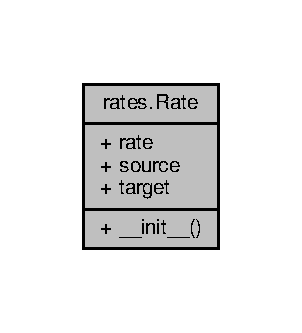
\includegraphics[width=145pt]{classrates_1_1_rate__coll__graph}
\end{center}
\end{figure}
\subsection*{Public Member Functions}
\begin{DoxyCompactItemize}
\item 
def \hyperlink{classrates_1_1_rate_a935221ad61f9c683e6da812ac7f53cc3}{\+\_\+\+\_\+init\+\_\+\+\_\+} (self, \hyperlink{classrates_1_1_rate_a82a6abb7536f2a4393f43456cfb1dc5e}{source}, \hyperlink{classrates_1_1_rate_adb1bbb0977c838106cb181a5941612c8}{target}, \hyperlink{classrates_1_1_rate_a5a660cfdfaa515a6e5809492525d61a7}{rate})
\end{DoxyCompactItemize}
\subsection*{Public Attributes}
\begin{DoxyCompactItemize}
\item 
\hyperlink{classrates_1_1_rate_a5a660cfdfaa515a6e5809492525d61a7}{rate}
\item 
\hyperlink{classrates_1_1_rate_a82a6abb7536f2a4393f43456cfb1dc5e}{source}
\item 
\hyperlink{classrates_1_1_rate_adb1bbb0977c838106cb181a5941612c8}{target}
\end{DoxyCompactItemize}


\subsection{Detailed Description}


Definition at line \hyperlink{rates_8py_source_l00012}{12} of file \hyperlink{rates_8py_source}{rates.\+py}.



\subsection{Constructor \& Destructor Documentation}
\index{rates\+::\+Rate@{rates\+::\+Rate}!\+\_\+\+\_\+init\+\_\+\+\_\+@{\+\_\+\+\_\+init\+\_\+\+\_\+}}
\index{\+\_\+\+\_\+init\+\_\+\+\_\+@{\+\_\+\+\_\+init\+\_\+\+\_\+}!rates\+::\+Rate@{rates\+::\+Rate}}
\subsubsection[{\texorpdfstring{\+\_\+\+\_\+init\+\_\+\+\_\+(self, source, target, rate)}{__init__(self, source, target, rate)}}]{\setlength{\rightskip}{0pt plus 5cm}def rates.\+Rate.\+\_\+\+\_\+init\+\_\+\+\_\+ (
\begin{DoxyParamCaption}
\item[{}]{self, }
\item[{}]{source, }
\item[{}]{target, }
\item[{}]{rate}
\end{DoxyParamCaption}
)}\hypertarget{classrates_1_1_rate_a935221ad61f9c683e6da812ac7f53cc3}{}\label{classrates_1_1_rate_a935221ad61f9c683e6da812ac7f53cc3}


Definition at line \hyperlink{rates_8py_source_l00013}{13} of file \hyperlink{rates_8py_source}{rates.\+py}.


\begin{DoxyCode}
\hypertarget{classrates_1_1_rate.tex_l00013}{}\hyperlink{classrates_1_1_rate_a935221ad61f9c683e6da812ac7f53cc3}{00013}     \textcolor{keyword}{def }\hyperlink{classrates_1_1_rate_a935221ad61f9c683e6da812ac7f53cc3}{\_\_init\_\_} (self, source, target, rate): 
\hypertarget{classrates_1_1_rate.tex_l00014}{}\hyperlink{classrates_1_1_rate_a82a6abb7536f2a4393f43456cfb1dc5e}{00014}         self.\hyperlink{classrates_1_1_rate_a82a6abb7536f2a4393f43456cfb1dc5e}{source} = source
\hypertarget{classrates_1_1_rate.tex_l00015}{}\hyperlink{classrates_1_1_rate_adb1bbb0977c838106cb181a5941612c8}{00015}         self.\hyperlink{classrates_1_1_rate_adb1bbb0977c838106cb181a5941612c8}{target} = target
\hypertarget{classrates_1_1_rate.tex_l00016}{}\hyperlink{classrates_1_1_rate_a5a660cfdfaa515a6e5809492525d61a7}{00016}         self.\hyperlink{classrates_1_1_rate_a5a660cfdfaa515a6e5809492525d61a7}{rate}   = rate        
00017         
\end{DoxyCode}


\subsection{Member Data Documentation}
\index{rates\+::\+Rate@{rates\+::\+Rate}!rate@{rate}}
\index{rate@{rate}!rates\+::\+Rate@{rates\+::\+Rate}}
\subsubsection[{\texorpdfstring{rate}{rate}}]{\setlength{\rightskip}{0pt plus 5cm}rates.\+Rate.\+rate}\hypertarget{classrates_1_1_rate_a5a660cfdfaa515a6e5809492525d61a7}{}\label{classrates_1_1_rate_a5a660cfdfaa515a6e5809492525d61a7}


Definition at line \hyperlink{rates_8py_source_l00016}{16} of file \hyperlink{rates_8py_source}{rates.\+py}.

\index{rates\+::\+Rate@{rates\+::\+Rate}!source@{source}}
\index{source@{source}!rates\+::\+Rate@{rates\+::\+Rate}}
\subsubsection[{\texorpdfstring{source}{source}}]{\setlength{\rightskip}{0pt plus 5cm}rates.\+Rate.\+source}\hypertarget{classrates_1_1_rate_a82a6abb7536f2a4393f43456cfb1dc5e}{}\label{classrates_1_1_rate_a82a6abb7536f2a4393f43456cfb1dc5e}


Definition at line \hyperlink{rates_8py_source_l00014}{14} of file \hyperlink{rates_8py_source}{rates.\+py}.

\index{rates\+::\+Rate@{rates\+::\+Rate}!target@{target}}
\index{target@{target}!rates\+::\+Rate@{rates\+::\+Rate}}
\subsubsection[{\texorpdfstring{target}{target}}]{\setlength{\rightskip}{0pt plus 5cm}rates.\+Rate.\+target}\hypertarget{classrates_1_1_rate_adb1bbb0977c838106cb181a5941612c8}{}\label{classrates_1_1_rate_adb1bbb0977c838106cb181a5941612c8}


Definition at line \hyperlink{rates_8py_source_l00015}{15} of file \hyperlink{rates_8py_source}{rates.\+py}.



The documentation for this class was generated from the following file\+:\begin{DoxyCompactItemize}
\item 
/home/hilton/github/exch2exh/\hyperlink{rates_8py}{rates.\+py}\end{DoxyCompactItemize}

\hypertarget{classexch2exch_1_1_rates}{\section{exch2exch.\-Rates Class Reference}
\label{classexch2exch_1_1_rates}\index{exch2exch.\-Rates@{exch2exch.\-Rates}}
}
\subsection*{Public Member Functions}
\begin{DoxyCompactItemize}
\item 
def \hyperlink{classexch2exch_1_1_rates_adf2f5038d3b15e4b434ae3d32527ebe2}{\-\_\-\-\_\-init\-\_\-\-\_\-}
\item 
def \hyperlink{classexch2exch_1_1_rates_ae5e570daf9d176e3455bc98fc19e2b2c}{get\-Brl2\-Usd}
\item 
def \hyperlink{classexch2exch_1_1_rates_a1b3705806d2321660c4c2753474f403d}{get\-Usd2\-Brl}
\item 
def \hyperlink{classexch2exch_1_1_rates_a8ec48a9ebb71f923056205ad79679eeb}{get\-Service\-Name}
\item 
def \hyperlink{classexch2exch_1_1_rates_ac50b5d57f05657995ea0152bc4f195e9}{\-\_\-\-\_\-str\-\_\-\-\_\-}
\end{DoxyCompactItemize}
\subsection*{Public Attributes}
\begin{DoxyCompactItemize}
\item 
\hyperlink{classexch2exch_1_1_rates_acb12f83bce4393714ec30351a1d636c2}{dt}
\item 
\hyperlink{classexch2exch_1_1_rates_ab79ad6e4a42ca358e6b39c825a4b8a0b}{usd2brl}
\item 
\hyperlink{classexch2exch_1_1_rates_acc018dea09e825e18e91c73c5c63ab78}{brl2usd}
\item 
\hyperlink{classexch2exch_1_1_rates_a94c1394b9259d6a7c8f3c12bbd20e685}{service}
\end{DoxyCompactItemize}


\subsection{Detailed Description}


Definition at line 26 of file exch2exch.\-py.



\subsection{Constructor \& Destructor Documentation}
\hypertarget{classexch2exch_1_1_rates_adf2f5038d3b15e4b434ae3d32527ebe2}{\index{exch2exch\-::\-Rates@{exch2exch\-::\-Rates}!\-\_\-\-\_\-init\-\_\-\-\_\-@{\-\_\-\-\_\-init\-\_\-\-\_\-}}
\index{\-\_\-\-\_\-init\-\_\-\-\_\-@{\-\_\-\-\_\-init\-\_\-\-\_\-}!exch2exch::Rates@{exch2exch\-::\-Rates}}
\subsubsection[{\-\_\-\-\_\-init\-\_\-\-\_\-}]{\setlength{\rightskip}{0pt plus 5cm}def exch2exch.\-Rates.\-\_\-\-\_\-init\-\_\-\-\_\- (
\begin{DoxyParamCaption}
\item[{}]{self, }
\item[{}]{dt, }
\item[{}]{usd2brl, }
\item[{}]{brl2usd, }
\item[{}]{service}
\end{DoxyParamCaption}
)}}\label{classexch2exch_1_1_rates_adf2f5038d3b15e4b434ae3d32527ebe2}


Definition at line 27 of file exch2exch.\-py.


\begin{DoxyCode}
27 
28     \textcolor{keyword}{def }\hyperlink{classexch2exch_1_1_rates_adf2f5038d3b15e4b434ae3d32527ebe2}{\_\_init\_\_} (self, dt, usd2brl, brl2usd, service):
29         self.\hyperlink{classexch2exch_1_1_rates_acb12f83bce4393714ec30351a1d636c2}{dt}  = dt
30         self.\hyperlink{classexch2exch_1_1_rates_ab79ad6e4a42ca358e6b39c825a4b8a0b}{usd2brl} = usd2brl
31         self.\hyperlink{classexch2exch_1_1_rates_acc018dea09e825e18e91c73c5c63ab78}{brl2usd} = brl2usd
32         self.\hyperlink{classexch2exch_1_1_rates_a94c1394b9259d6a7c8f3c12bbd20e685}{service} = service
    
\end{DoxyCode}


\subsection{Member Function Documentation}
\hypertarget{classexch2exch_1_1_rates_ac50b5d57f05657995ea0152bc4f195e9}{\index{exch2exch\-::\-Rates@{exch2exch\-::\-Rates}!\-\_\-\-\_\-str\-\_\-\-\_\-@{\-\_\-\-\_\-str\-\_\-\-\_\-}}
\index{\-\_\-\-\_\-str\-\_\-\-\_\-@{\-\_\-\-\_\-str\-\_\-\-\_\-}!exch2exch::Rates@{exch2exch\-::\-Rates}}
\subsubsection[{\-\_\-\-\_\-str\-\_\-\-\_\-}]{\setlength{\rightskip}{0pt plus 5cm}def exch2exch.\-Rates.\-\_\-\-\_\-str\-\_\-\-\_\- (
\begin{DoxyParamCaption}
\item[{}]{self}
\end{DoxyParamCaption}
)}}\label{classexch2exch_1_1_rates_ac50b5d57f05657995ea0152bc4f195e9}


Definition at line 42 of file exch2exch.\-py.



References exch2exch.\-Rates.\-brl2usd, exch2exch.\-Rates.\-dt, exch2exch.\-Rates.\-service, and exch2exch.\-Rates.\-usd2brl.


\begin{DoxyCode}
42 
43     \textcolor{keyword}{def }\hyperlink{classexch2exch_1_1_rates_ac50b5d57f05657995ea0152bc4f195e9}{\_\_str\_\_} (self):
44         result = \textcolor{stringliteral}{''}
45 
46         service = self.\hyperlink{classexch2exch_1_1_rates_a94c1394b9259d6a7c8f3c12bbd20e685}{service}
47         dt      = self.\hyperlink{classexch2exch_1_1_rates_acb12f83bce4393714ec30351a1d636c2}{dt}
48         usd2brl = self.\hyperlink{classexch2exch_1_1_rates_ab79ad6e4a42ca358e6b39c825a4b8a0b}{usd2brl}
49         brl2usd = self.\hyperlink{classexch2exch_1_1_rates_acc018dea09e825e18e91c73c5c63ab78}{brl2usd}
50         ftupl = (service, dt, usd2brl, brl2usd)
51         
52         result = \textcolor{stringliteral}{"\{0\}: \{1\}: USD2BRL \{2:.4f\}, BRL2USD \{3:.4f\}"}.format (*ftupl)
53 
54         \textcolor{keywordflow}{return} result        
        
\end{DoxyCode}
\hypertarget{classexch2exch_1_1_rates_ae5e570daf9d176e3455bc98fc19e2b2c}{\index{exch2exch\-::\-Rates@{exch2exch\-::\-Rates}!get\-Brl2\-Usd@{get\-Brl2\-Usd}}
\index{get\-Brl2\-Usd@{get\-Brl2\-Usd}!exch2exch::Rates@{exch2exch\-::\-Rates}}
\subsubsection[{get\-Brl2\-Usd}]{\setlength{\rightskip}{0pt plus 5cm}def exch2exch.\-Rates.\-get\-Brl2\-Usd (
\begin{DoxyParamCaption}
\item[{}]{self}
\end{DoxyParamCaption}
)}}\label{classexch2exch_1_1_rates_ae5e570daf9d176e3455bc98fc19e2b2c}


Definition at line 33 of file exch2exch.\-py.



References exch2exch.\-Rates.\-brl2usd.


\begin{DoxyCode}
33 
34     \textcolor{keyword}{def }\hyperlink{classexch2exch_1_1_rates_ae5e570daf9d176e3455bc98fc19e2b2c}{getBrl2Usd} (self):
35         \textcolor{keywordflow}{return} self.\hyperlink{classexch2exch_1_1_rates_acc018dea09e825e18e91c73c5c63ab78}{brl2usd}
    
\end{DoxyCode}
\hypertarget{classexch2exch_1_1_rates_a8ec48a9ebb71f923056205ad79679eeb}{\index{exch2exch\-::\-Rates@{exch2exch\-::\-Rates}!get\-Service\-Name@{get\-Service\-Name}}
\index{get\-Service\-Name@{get\-Service\-Name}!exch2exch::Rates@{exch2exch\-::\-Rates}}
\subsubsection[{get\-Service\-Name}]{\setlength{\rightskip}{0pt plus 5cm}def exch2exch.\-Rates.\-get\-Service\-Name (
\begin{DoxyParamCaption}
\item[{}]{self}
\end{DoxyParamCaption}
)}}\label{classexch2exch_1_1_rates_a8ec48a9ebb71f923056205ad79679eeb}


Definition at line 39 of file exch2exch.\-py.



References exch2exch.\-Rates.\-service.


\begin{DoxyCode}
39 
40     \textcolor{keyword}{def }\hyperlink{classexch2exch_1_1_rates_a8ec48a9ebb71f923056205ad79679eeb}{getServiceName} (self):
41         \textcolor{keywordflow}{return} self.\hyperlink{classexch2exch_1_1_rates_a94c1394b9259d6a7c8f3c12bbd20e685}{service}
        
\end{DoxyCode}
\hypertarget{classexch2exch_1_1_rates_a1b3705806d2321660c4c2753474f403d}{\index{exch2exch\-::\-Rates@{exch2exch\-::\-Rates}!get\-Usd2\-Brl@{get\-Usd2\-Brl}}
\index{get\-Usd2\-Brl@{get\-Usd2\-Brl}!exch2exch::Rates@{exch2exch\-::\-Rates}}
\subsubsection[{get\-Usd2\-Brl}]{\setlength{\rightskip}{0pt plus 5cm}def exch2exch.\-Rates.\-get\-Usd2\-Brl (
\begin{DoxyParamCaption}
\item[{}]{self}
\end{DoxyParamCaption}
)}}\label{classexch2exch_1_1_rates_a1b3705806d2321660c4c2753474f403d}


Definition at line 36 of file exch2exch.\-py.



References exch2exch.\-Rates.\-usd2brl.


\begin{DoxyCode}
36 
37     \textcolor{keyword}{def }\hyperlink{classexch2exch_1_1_rates_a1b3705806d2321660c4c2753474f403d}{getUsd2Brl} (self):
38         \textcolor{keywordflow}{return} self.\hyperlink{classexch2exch_1_1_rates_ab79ad6e4a42ca358e6b39c825a4b8a0b}{usd2brl}
    
\end{DoxyCode}


\subsection{Member Data Documentation}
\hypertarget{classexch2exch_1_1_rates_acc018dea09e825e18e91c73c5c63ab78}{\index{exch2exch\-::\-Rates@{exch2exch\-::\-Rates}!brl2usd@{brl2usd}}
\index{brl2usd@{brl2usd}!exch2exch::Rates@{exch2exch\-::\-Rates}}
\subsubsection[{brl2usd}]{\setlength{\rightskip}{0pt plus 5cm}exch2exch.\-Rates.\-brl2usd}}\label{classexch2exch_1_1_rates_acc018dea09e825e18e91c73c5c63ab78}


Definition at line 30 of file exch2exch.\-py.



Referenced by raw\-\_\-urlparser.\-Rates.\-\_\-\-\_\-str\-\_\-\-\_\-(), exch2exch.\-Rates.\-\_\-\-\_\-str\-\_\-\-\_\-(), raw\-\_\-urlparser.\-Rates.\-get\-Brl2\-Usd(), and exch2exch.\-Rates.\-get\-Brl2\-Usd().

\hypertarget{classexch2exch_1_1_rates_acb12f83bce4393714ec30351a1d636c2}{\index{exch2exch\-::\-Rates@{exch2exch\-::\-Rates}!dt@{dt}}
\index{dt@{dt}!exch2exch::Rates@{exch2exch\-::\-Rates}}
\subsubsection[{dt}]{\setlength{\rightskip}{0pt plus 5cm}exch2exch.\-Rates.\-dt}}\label{classexch2exch_1_1_rates_acb12f83bce4393714ec30351a1d636c2}


Definition at line 28 of file exch2exch.\-py.



Referenced by raw\-\_\-urlparser.\-Rates.\-\_\-\-\_\-str\-\_\-\-\_\-(), exch2exch.\-Rates.\-\_\-\-\_\-str\-\_\-\-\_\-(), raw\-\_\-urlparser.\-Xbt\-Prices.\-\_\-\-\_\-str\-\_\-\-\_\-(), exch2exch.\-Xbt\-Prices.\-\_\-\-\_\-str\-\_\-\-\_\-(), exchange.\-Fox\-Bit.\-get\-\_\-ticker(), exchange.\-Mercado\-Bitcoin.\-get\-\_\-ticker(), exchange.\-Ok\-Coin.\-get\-\_\-ticker(), raw\-\_\-urlparser.\-Xbt\-Prices.\-get\-Date\-Time(), and exch2exch.\-Xbt\-Prices.\-get\-Date\-Time().

\hypertarget{classexch2exch_1_1_rates_a94c1394b9259d6a7c8f3c12bbd20e685}{\index{exch2exch\-::\-Rates@{exch2exch\-::\-Rates}!service@{service}}
\index{service@{service}!exch2exch::Rates@{exch2exch\-::\-Rates}}
\subsubsection[{service}]{\setlength{\rightskip}{0pt plus 5cm}exch2exch.\-Rates.\-service}}\label{classexch2exch_1_1_rates_a94c1394b9259d6a7c8f3c12bbd20e685}


Definition at line 31 of file exch2exch.\-py.



Referenced by raw\-\_\-urlparser.\-Rates.\-\_\-\-\_\-str\-\_\-\-\_\-(), exch2exch.\-Rates.\-\_\-\-\_\-str\-\_\-\-\_\-(), raw\-\_\-urlparser.\-Rates.\-get\-Service\-Name(), and exch2exch.\-Rates.\-get\-Service\-Name().

\hypertarget{classexch2exch_1_1_rates_ab79ad6e4a42ca358e6b39c825a4b8a0b}{\index{exch2exch\-::\-Rates@{exch2exch\-::\-Rates}!usd2brl@{usd2brl}}
\index{usd2brl@{usd2brl}!exch2exch::Rates@{exch2exch\-::\-Rates}}
\subsubsection[{usd2brl}]{\setlength{\rightskip}{0pt plus 5cm}exch2exch.\-Rates.\-usd2brl}}\label{classexch2exch_1_1_rates_ab79ad6e4a42ca358e6b39c825a4b8a0b}


Definition at line 29 of file exch2exch.\-py.



Referenced by raw\-\_\-urlparser.\-Rates.\-\_\-\-\_\-str\-\_\-\-\_\-(), exch2exch.\-Rates.\-\_\-\-\_\-str\-\_\-\-\_\-(), raw\-\_\-urlparser.\-Rates.\-get\-Usd2\-Brl(), and exch2exch.\-Rates.\-get\-Usd2\-Brl().



The documentation for this class was generated from the following file\-:\begin{DoxyCompactItemize}
\item 
/home/hilton/github/exch2exh/\hyperlink{exch2exch_8py}{exch2exch.\-py}\end{DoxyCompactItemize}

\hypertarget{classrates_1_1_rates}{}\section{rates.\+Rates Class Reference}
\label{classrates_1_1_rates}\index{rates.\+Rates@{rates.\+Rates}}


Inheritance diagram for rates.\+Rates\+:
\nopagebreak
\begin{figure}[H]
\begin{center}
\leavevmode
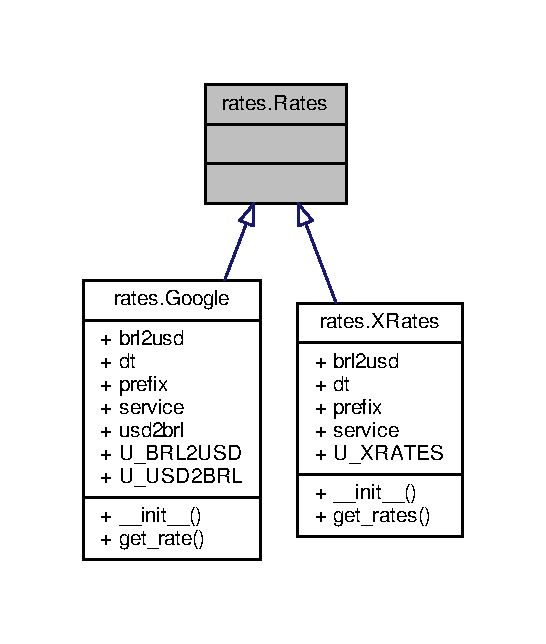
\includegraphics[width=262pt]{classrates_1_1_rates__inherit__graph}
\end{center}
\end{figure}


Collaboration diagram for rates.\+Rates\+:
\nopagebreak
\begin{figure}[H]
\begin{center}
\leavevmode
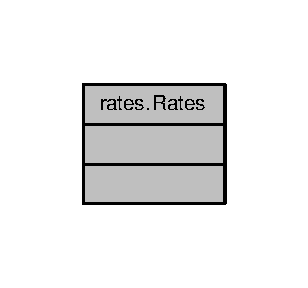
\includegraphics[width=148pt]{classrates_1_1_rates__coll__graph}
\end{center}
\end{figure}


\subsection{Detailed Description}


Definition at line \hyperlink{rates_8py_source_l00018}{18} of file \hyperlink{rates_8py_source}{rates.\+py}.



The documentation for this class was generated from the following file\+:\begin{DoxyCompactItemize}
\item 
/home/hilton/github/exch2exh/\hyperlink{rates_8py}{rates.\+py}\end{DoxyCompactItemize}

\hypertarget{classraw__urlparser_1_1_rates}{\section{raw\-\_\-urlparser.\-Rates Class Reference}
\label{classraw__urlparser_1_1_rates}\index{raw\-\_\-urlparser.\-Rates@{raw\-\_\-urlparser.\-Rates}}
}
\subsection*{Public Member Functions}
\begin{DoxyCompactItemize}
\item 
def \hyperlink{classraw__urlparser_1_1_rates_a2de6334a686a8a81c619d99de46e43df}{\-\_\-\-\_\-init\-\_\-\-\_\-}
\item 
def \hyperlink{classraw__urlparser_1_1_rates_a166ead3ebf1546ec2ea3eb299d524a30}{\-\_\-\-\_\-str\-\_\-\-\_\-}
\item 
def \hyperlink{classraw__urlparser_1_1_rates_a435ff5562321da275bb95823a346bc5c}{get\-Brl2\-Usd}
\item 
def \hyperlink{classraw__urlparser_1_1_rates_a4579624e853a4d83c5b7df9c390de5b5}{get\-Service\-Name}
\item 
def \hyperlink{classraw__urlparser_1_1_rates_aaf3f32369f17da5fc903a7a51feca25f}{get\-Usd2\-Brl}
\end{DoxyCompactItemize}
\subsection*{Public Attributes}
\begin{DoxyCompactItemize}
\item 
\hyperlink{classraw__urlparser_1_1_rates_adc9df007bec75344f9f89cb631d1aeb3}{brl2usd}
\item 
\hyperlink{classraw__urlparser_1_1_rates_a09b3c7cb595f3135c3eda648b1bb4c3f}{dt}
\item 
\hyperlink{classraw__urlparser_1_1_rates_acb05316e95a39bc42590a882712f854b}{service}
\item 
\hyperlink{classraw__urlparser_1_1_rates_a52d9b688be8385a87783b27839749b4a}{usd2brl}
\end{DoxyCompactItemize}


\subsection{Detailed Description}


Definition at line 22 of file raw\-\_\-urlparser.\-py.



\subsection{Constructor \& Destructor Documentation}
\hypertarget{classraw__urlparser_1_1_rates_a2de6334a686a8a81c619d99de46e43df}{\index{raw\-\_\-urlparser\-::\-Rates@{raw\-\_\-urlparser\-::\-Rates}!\-\_\-\-\_\-init\-\_\-\-\_\-@{\-\_\-\-\_\-init\-\_\-\-\_\-}}
\index{\-\_\-\-\_\-init\-\_\-\-\_\-@{\-\_\-\-\_\-init\-\_\-\-\_\-}!raw_urlparser::Rates@{raw\-\_\-urlparser\-::\-Rates}}
\subsubsection[{\-\_\-\-\_\-init\-\_\-\-\_\-}]{\setlength{\rightskip}{0pt plus 5cm}def raw\-\_\-urlparser.\-Rates.\-\_\-\-\_\-init\-\_\-\-\_\- (
\begin{DoxyParamCaption}
\item[{}]{self, }
\item[{}]{dt, }
\item[{}]{usd2brl, }
\item[{}]{brl2usd, }
\item[{}]{service}
\end{DoxyParamCaption}
)}}\label{classraw__urlparser_1_1_rates_a2de6334a686a8a81c619d99de46e43df}


Definition at line 23 of file raw\-\_\-urlparser.\-py.


\begin{DoxyCode}
23 
24     \textcolor{keyword}{def }\hyperlink{classraw__urlparser_1_1_rates_a2de6334a686a8a81c619d99de46e43df}{\_\_init\_\_} (self, dt, usd2brl, brl2usd, service):
25         self.\hyperlink{classraw__urlparser_1_1_rates_a09b3c7cb595f3135c3eda648b1bb4c3f}{dt}  = dt
26         self.\hyperlink{classraw__urlparser_1_1_rates_a52d9b688be8385a87783b27839749b4a}{usd2brl} = usd2brl
27         self.\hyperlink{classraw__urlparser_1_1_rates_adc9df007bec75344f9f89cb631d1aeb3}{brl2usd} = brl2usd
28         self.\hyperlink{classraw__urlparser_1_1_rates_acb05316e95a39bc42590a882712f854b}{service} = service
    
\end{DoxyCode}


\subsection{Member Function Documentation}
\hypertarget{classraw__urlparser_1_1_rates_a166ead3ebf1546ec2ea3eb299d524a30}{\index{raw\-\_\-urlparser\-::\-Rates@{raw\-\_\-urlparser\-::\-Rates}!\-\_\-\-\_\-str\-\_\-\-\_\-@{\-\_\-\-\_\-str\-\_\-\-\_\-}}
\index{\-\_\-\-\_\-str\-\_\-\-\_\-@{\-\_\-\-\_\-str\-\_\-\-\_\-}!raw_urlparser::Rates@{raw\-\_\-urlparser\-::\-Rates}}
\subsubsection[{\-\_\-\-\_\-str\-\_\-\-\_\-}]{\setlength{\rightskip}{0pt plus 5cm}def raw\-\_\-urlparser.\-Rates.\-\_\-\-\_\-str\-\_\-\-\_\- (
\begin{DoxyParamCaption}
\item[{}]{self}
\end{DoxyParamCaption}
)}}\label{classraw__urlparser_1_1_rates_a166ead3ebf1546ec2ea3eb299d524a30}


Definition at line 38 of file raw\-\_\-urlparser.\-py.



References raw\-\_\-urlparser.\-Rates.\-brl2usd, exch2exch.\-Rates.\-brl2usd, raw\-\_\-urlparser.\-Rates.\-dt, exch2exch.\-Rates.\-dt, exch2exch.\-Xbt\-Prices.\-dt, exchange.\-Fox\-Bit.\-dt, exchange.\-Mercado\-Bitcoin.\-dt, exchange.\-Ok\-Coin.\-dt, raw\-\_\-urlparser.\-Rates.\-service, exch2exch.\-Rates.\-service, raw\-\_\-urlparser.\-Rates.\-usd2brl, and exch2exch.\-Rates.\-usd2brl.


\begin{DoxyCode}
38 
39     \textcolor{keyword}{def }\hyperlink{classraw__urlparser_1_1_rates_a166ead3ebf1546ec2ea3eb299d524a30}{\_\_str\_\_} (self):
40         result = \textcolor{stringliteral}{''}
41 
42         service = self.\hyperlink{classraw__urlparser_1_1_rates_acb05316e95a39bc42590a882712f854b}{service}
43         dt      = self.\hyperlink{classraw__urlparser_1_1_rates_a09b3c7cb595f3135c3eda648b1bb4c3f}{dt}
44         usd2brl = self.\hyperlink{classraw__urlparser_1_1_rates_a52d9b688be8385a87783b27839749b4a}{usd2brl}
45         brl2usd = self.\hyperlink{classraw__urlparser_1_1_rates_adc9df007bec75344f9f89cb631d1aeb3}{brl2usd}
46         ftupl = (service, dt, usd2brl, brl2usd)
47         
48         result = \textcolor{stringliteral}{"\{0\}: \{1\}: USD2BRL \{2:.4f\}, BRL2USD \{3:.4f\}"}.format (*ftupl)
49 
50         \textcolor{keywordflow}{return} result        
        
\end{DoxyCode}
\hypertarget{classraw__urlparser_1_1_rates_a435ff5562321da275bb95823a346bc5c}{\index{raw\-\_\-urlparser\-::\-Rates@{raw\-\_\-urlparser\-::\-Rates}!get\-Brl2\-Usd@{get\-Brl2\-Usd}}
\index{get\-Brl2\-Usd@{get\-Brl2\-Usd}!raw_urlparser::Rates@{raw\-\_\-urlparser\-::\-Rates}}
\subsubsection[{get\-Brl2\-Usd}]{\setlength{\rightskip}{0pt plus 5cm}def raw\-\_\-urlparser.\-Rates.\-get\-Brl2\-Usd (
\begin{DoxyParamCaption}
\item[{}]{self}
\end{DoxyParamCaption}
)}}\label{classraw__urlparser_1_1_rates_a435ff5562321da275bb95823a346bc5c}


Definition at line 29 of file raw\-\_\-urlparser.\-py.



References raw\-\_\-urlparser.\-Rates.\-brl2usd, and exch2exch.\-Rates.\-brl2usd.


\begin{DoxyCode}
29 
30     \textcolor{keyword}{def }\hyperlink{classraw__urlparser_1_1_rates_a435ff5562321da275bb95823a346bc5c}{getBrl2Usd} (self):
31         \textcolor{keywordflow}{return} self.\hyperlink{classraw__urlparser_1_1_rates_adc9df007bec75344f9f89cb631d1aeb3}{brl2usd}
    
\end{DoxyCode}
\hypertarget{classraw__urlparser_1_1_rates_a4579624e853a4d83c5b7df9c390de5b5}{\index{raw\-\_\-urlparser\-::\-Rates@{raw\-\_\-urlparser\-::\-Rates}!get\-Service\-Name@{get\-Service\-Name}}
\index{get\-Service\-Name@{get\-Service\-Name}!raw_urlparser::Rates@{raw\-\_\-urlparser\-::\-Rates}}
\subsubsection[{get\-Service\-Name}]{\setlength{\rightskip}{0pt plus 5cm}def raw\-\_\-urlparser.\-Rates.\-get\-Service\-Name (
\begin{DoxyParamCaption}
\item[{}]{self}
\end{DoxyParamCaption}
)}}\label{classraw__urlparser_1_1_rates_a4579624e853a4d83c5b7df9c390de5b5}


Definition at line 35 of file raw\-\_\-urlparser.\-py.



References raw\-\_\-urlparser.\-Rates.\-service, and exch2exch.\-Rates.\-service.


\begin{DoxyCode}
35 
36     \textcolor{keyword}{def }\hyperlink{classraw__urlparser_1_1_rates_a4579624e853a4d83c5b7df9c390de5b5}{getServiceName} (self):
37         \textcolor{keywordflow}{return} self.\hyperlink{classraw__urlparser_1_1_rates_acb05316e95a39bc42590a882712f854b}{service}
        
\end{DoxyCode}
\hypertarget{classraw__urlparser_1_1_rates_aaf3f32369f17da5fc903a7a51feca25f}{\index{raw\-\_\-urlparser\-::\-Rates@{raw\-\_\-urlparser\-::\-Rates}!get\-Usd2\-Brl@{get\-Usd2\-Brl}}
\index{get\-Usd2\-Brl@{get\-Usd2\-Brl}!raw_urlparser::Rates@{raw\-\_\-urlparser\-::\-Rates}}
\subsubsection[{get\-Usd2\-Brl}]{\setlength{\rightskip}{0pt plus 5cm}def raw\-\_\-urlparser.\-Rates.\-get\-Usd2\-Brl (
\begin{DoxyParamCaption}
\item[{}]{self}
\end{DoxyParamCaption}
)}}\label{classraw__urlparser_1_1_rates_aaf3f32369f17da5fc903a7a51feca25f}


Definition at line 32 of file raw\-\_\-urlparser.\-py.



References raw\-\_\-urlparser.\-Rates.\-usd2brl, and exch2exch.\-Rates.\-usd2brl.


\begin{DoxyCode}
32 
33     \textcolor{keyword}{def }\hyperlink{classraw__urlparser_1_1_rates_aaf3f32369f17da5fc903a7a51feca25f}{getUsd2Brl} (self):
34         \textcolor{keywordflow}{return} self.\hyperlink{classraw__urlparser_1_1_rates_a52d9b688be8385a87783b27839749b4a}{usd2brl}
    
\end{DoxyCode}


\subsection{Member Data Documentation}
\hypertarget{classraw__urlparser_1_1_rates_adc9df007bec75344f9f89cb631d1aeb3}{\index{raw\-\_\-urlparser\-::\-Rates@{raw\-\_\-urlparser\-::\-Rates}!brl2usd@{brl2usd}}
\index{brl2usd@{brl2usd}!raw_urlparser::Rates@{raw\-\_\-urlparser\-::\-Rates}}
\subsubsection[{brl2usd}]{\setlength{\rightskip}{0pt plus 5cm}raw\-\_\-urlparser.\-Rates.\-brl2usd}}\label{classraw__urlparser_1_1_rates_adc9df007bec75344f9f89cb631d1aeb3}


Definition at line 26 of file raw\-\_\-urlparser.\-py.



Referenced by raw\-\_\-urlparser.\-Rates.\-\_\-\-\_\-str\-\_\-\-\_\-(), and raw\-\_\-urlparser.\-Rates.\-get\-Brl2\-Usd().

\hypertarget{classraw__urlparser_1_1_rates_a09b3c7cb595f3135c3eda648b1bb4c3f}{\index{raw\-\_\-urlparser\-::\-Rates@{raw\-\_\-urlparser\-::\-Rates}!dt@{dt}}
\index{dt@{dt}!raw_urlparser::Rates@{raw\-\_\-urlparser\-::\-Rates}}
\subsubsection[{dt}]{\setlength{\rightskip}{0pt plus 5cm}raw\-\_\-urlparser.\-Rates.\-dt}}\label{classraw__urlparser_1_1_rates_a09b3c7cb595f3135c3eda648b1bb4c3f}


Definition at line 24 of file raw\-\_\-urlparser.\-py.



Referenced by raw\-\_\-urlparser.\-Rates.\-\_\-\-\_\-str\-\_\-\-\_\-(), raw\-\_\-urlparser.\-Xbt\-Prices.\-\_\-\-\_\-str\-\_\-\-\_\-(), and raw\-\_\-urlparser.\-Xbt\-Prices.\-get\-Date\-Time().

\hypertarget{classraw__urlparser_1_1_rates_acb05316e95a39bc42590a882712f854b}{\index{raw\-\_\-urlparser\-::\-Rates@{raw\-\_\-urlparser\-::\-Rates}!service@{service}}
\index{service@{service}!raw_urlparser::Rates@{raw\-\_\-urlparser\-::\-Rates}}
\subsubsection[{service}]{\setlength{\rightskip}{0pt plus 5cm}raw\-\_\-urlparser.\-Rates.\-service}}\label{classraw__urlparser_1_1_rates_acb05316e95a39bc42590a882712f854b}


Definition at line 27 of file raw\-\_\-urlparser.\-py.



Referenced by raw\-\_\-urlparser.\-Rates.\-\_\-\-\_\-str\-\_\-\-\_\-(), and raw\-\_\-urlparser.\-Rates.\-get\-Service\-Name().

\hypertarget{classraw__urlparser_1_1_rates_a52d9b688be8385a87783b27839749b4a}{\index{raw\-\_\-urlparser\-::\-Rates@{raw\-\_\-urlparser\-::\-Rates}!usd2brl@{usd2brl}}
\index{usd2brl@{usd2brl}!raw_urlparser::Rates@{raw\-\_\-urlparser\-::\-Rates}}
\subsubsection[{usd2brl}]{\setlength{\rightskip}{0pt plus 5cm}raw\-\_\-urlparser.\-Rates.\-usd2brl}}\label{classraw__urlparser_1_1_rates_a52d9b688be8385a87783b27839749b4a}


Definition at line 25 of file raw\-\_\-urlparser.\-py.



Referenced by raw\-\_\-urlparser.\-Rates.\-\_\-\-\_\-str\-\_\-\-\_\-(), and raw\-\_\-urlparser.\-Rates.\-get\-Usd2\-Brl().



The documentation for this class was generated from the following file\-:\begin{DoxyCompactItemize}
\item 
/home/hilton/github/exch2exh/\hyperlink{raw__urlparser_8py}{raw\-\_\-urlparser.\-py}\end{DoxyCompactItemize}

\hypertarget{classexchange_1_1_ticker}{}\section{exchange.\+Ticker Class Reference}
\label{classexchange_1_1_ticker}\index{exchange.\+Ticker@{exchange.\+Ticker}}


Collaboration diagram for exchange.\+Ticker\+:\nopagebreak
\begin{figure}[H]
\begin{center}
\leavevmode
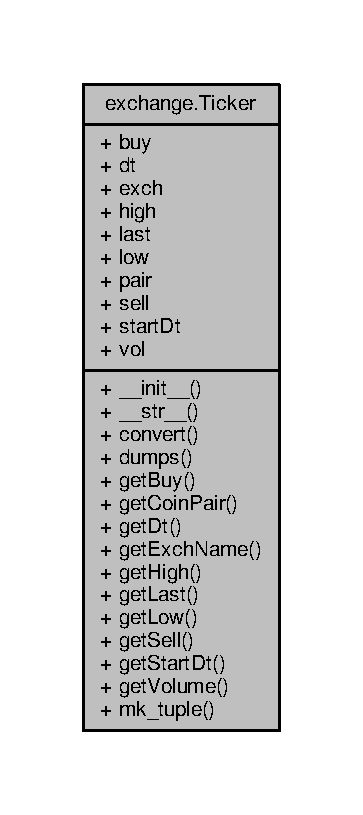
\includegraphics[width=169pt]{classexchange_1_1_ticker__coll__graph}
\end{center}
\end{figure}
\subsection*{Public Member Functions}
\begin{DoxyCompactItemize}
\item 
def \hyperlink{classexchange_1_1_ticker_a4a8c99ada461a4aeb960c14020a47736}{\+\_\+\+\_\+init\+\_\+\+\_\+} (self, \hyperlink{classexchange_1_1_ticker_a33f33fe9a12da3ce52938afdc577c061}{exch}, \hyperlink{classexchange_1_1_ticker_a382f9199d13a7b5929a26065fad4e491}{pair}, \hyperlink{classexchange_1_1_ticker_a45e3162d9956cee797f21d93c44c6baf}{dt}, \hyperlink{classexchange_1_1_ticker_a2ca48c3fa9aba92241392a05bef39324}{buy}, \hyperlink{classexchange_1_1_ticker_a5ba9e257d2ed28f02528a37d9ebd793e}{sell}, \hyperlink{classexchange_1_1_ticker_aace381ca15468df6a40e8d86b7710a7f}{high}, \hyperlink{classexchange_1_1_ticker_a1c1f26a47a82fc799fcebf158e104405}{low}, \hyperlink{classexchange_1_1_ticker_add7c2d95fa790dcdffddae2e584ce5f5}{last}, \hyperlink{classexchange_1_1_ticker_a24c0dd396aebc54c06e429a68c964ea3}{vol})
\begin{DoxyCompactList}\small\item\em Constructor. \end{DoxyCompactList}\item 
def \hyperlink{classexchange_1_1_ticker_af91836a1c408f54dda95d9865cefba45}{\+\_\+\+\_\+str\+\_\+\+\_\+} (self)
\item 
def \hyperlink{classexchange_1_1_ticker_a2aa851437f953462f8e8bce7ca05c3ec}{convert} (self, rate, destination)
\item 
def \hyperlink{classexchange_1_1_ticker_a53148d54a0b9b577870db785fb4e381e}{dumps} (self)
\item 
def \hyperlink{classexchange_1_1_ticker_aaa2f7d66782b9405c286e98bfb281d45}{get\+Dt} (self)
\item 
def \hyperlink{classexchange_1_1_ticker_ab31537c5a057f9a47839e2d28411c1cf}{get\+Exch} (self)
\item 
def \hyperlink{classexchange_1_1_ticker_a3600faedb720e664d6fdc89415c01678}{get\+Pair} (self)
\item 
def \hyperlink{classexchange_1_1_ticker_aba1398da3113a7ff17b2496ce92c7238}{mk\+\_\+tuple} (self)
\end{DoxyCompactItemize}
\subsection*{Public Attributes}
\begin{DoxyCompactItemize}
\item 
\hyperlink{classexchange_1_1_ticker_a2ca48c3fa9aba92241392a05bef39324}{buy}
\item 
\hyperlink{classexchange_1_1_ticker_a45e3162d9956cee797f21d93c44c6baf}{dt}
\item 
\hyperlink{classexchange_1_1_ticker_a33f33fe9a12da3ce52938afdc577c061}{exch}
\item 
\hyperlink{classexchange_1_1_ticker_aace381ca15468df6a40e8d86b7710a7f}{high}
\item 
\hyperlink{classexchange_1_1_ticker_add7c2d95fa790dcdffddae2e584ce5f5}{last}
\item 
\hyperlink{classexchange_1_1_ticker_a1c1f26a47a82fc799fcebf158e104405}{low}
\item 
\hyperlink{classexchange_1_1_ticker_a382f9199d13a7b5929a26065fad4e491}{pair}
\item 
\hyperlink{classexchange_1_1_ticker_a5ba9e257d2ed28f02528a37d9ebd793e}{sell}
\item 
\hyperlink{classexchange_1_1_ticker_a24c0dd396aebc54c06e429a68c964ea3}{vol}
\end{DoxyCompactItemize}


\subsection{Detailed Description}


Definition at line \hyperlink{exchange_8py_source_l00043}{43} of file \hyperlink{exchange_8py_source}{exchange.\+py}.



\subsection{Constructor \& Destructor Documentation}
\index{exchange\+::\+Ticker@{exchange\+::\+Ticker}!\+\_\+\+\_\+init\+\_\+\+\_\+@{\+\_\+\+\_\+init\+\_\+\+\_\+}}
\index{\+\_\+\+\_\+init\+\_\+\+\_\+@{\+\_\+\+\_\+init\+\_\+\+\_\+}!exchange\+::\+Ticker@{exchange\+::\+Ticker}}
\subsubsection[{\texorpdfstring{\+\_\+\+\_\+init\+\_\+\+\_\+(self, exch, pair, dt, buy, sell, high, low, last, vol)}{__init__(self, exch, pair, dt, buy, sell, high, low, last, vol)}}]{\setlength{\rightskip}{0pt plus 5cm}def exchange.\+Ticker.\+\_\+\+\_\+init\+\_\+\+\_\+ (
\begin{DoxyParamCaption}
\item[{}]{self, }
\item[{}]{exch, }
\item[{}]{pair, }
\item[{}]{dt, }
\item[{}]{buy, }
\item[{}]{sell, }
\item[{}]{high, }
\item[{}]{low, }
\item[{}]{last, }
\item[{}]{vol}
\end{DoxyParamCaption}
)}\hypertarget{classexchange_1_1_ticker_a4a8c99ada461a4aeb960c14020a47736}{}\label{classexchange_1_1_ticker_a4a8c99ada461a4aeb960c14020a47736}


Constructor. 


\begin{DoxyParams}{Parameters}
{\em exch} & Name of the exchange, a string not the object \\
\hline
{\em pair} & Pair of coins -- 1st target coin, 2nd source coin \\
\hline
{\em dt} & Date and time as seconds since 1970/01/01 at zero hours \\
\hline
{\em buy} & Bid price \\
\hline
{\em sell} & Ask price \\
\hline
{\em high} & Highest price traded \\
\hline
{\em low} & Lowest price traded \\
\hline
{\em last} & Price of last trade \\
\hline
{\em vol} & Volume traded \\
\hline
\end{DoxyParams}


Definition at line \hyperlink{exchange_8py_source_l00054}{54} of file \hyperlink{exchange_8py_source}{exchange.\+py}.


\begin{DoxyCode}
\hypertarget{classexchange_1_1_ticker.tex_l00054}{}\hyperlink{classexchange_1_1_ticker_a4a8c99ada461a4aeb960c14020a47736}{00054}     \textcolor{keyword}{def }\hyperlink{classexchange_1_1_ticker_a4a8c99ada461a4aeb960c14020a47736}{\_\_init\_\_} (self, exch, pair, dt, buy, sell, high, low, last, vol):
\hypertarget{classexchange_1_1_ticker.tex_l00055}{}\hyperlink{classexchange_1_1_ticker_a33f33fe9a12da3ce52938afdc577c061}{00055}         self.\hyperlink{classexchange_1_1_ticker_a33f33fe9a12da3ce52938afdc577c061}{exch} = exch
\hypertarget{classexchange_1_1_ticker.tex_l00056}{}\hyperlink{classexchange_1_1_ticker_a382f9199d13a7b5929a26065fad4e491}{00056}         self.\hyperlink{classexchange_1_1_ticker_a382f9199d13a7b5929a26065fad4e491}{pair} = pair
\hypertarget{classexchange_1_1_ticker.tex_l00057}{}\hyperlink{classexchange_1_1_ticker_a45e3162d9956cee797f21d93c44c6baf}{00057}         self.\hyperlink{classexchange_1_1_ticker_a45e3162d9956cee797f21d93c44c6baf}{dt}   = dt
\hypertarget{classexchange_1_1_ticker.tex_l00058}{}\hyperlink{classexchange_1_1_ticker_a2ca48c3fa9aba92241392a05bef39324}{00058}         self.\hyperlink{classexchange_1_1_ticker_a2ca48c3fa9aba92241392a05bef39324}{buy}  = buy 
\hypertarget{classexchange_1_1_ticker.tex_l00059}{}\hyperlink{classexchange_1_1_ticker_a5ba9e257d2ed28f02528a37d9ebd793e}{00059}         self.\hyperlink{classexchange_1_1_ticker_a5ba9e257d2ed28f02528a37d9ebd793e}{sell} = sell 
\hypertarget{classexchange_1_1_ticker.tex_l00060}{}\hyperlink{classexchange_1_1_ticker_aace381ca15468df6a40e8d86b7710a7f}{00060}         self.\hyperlink{classexchange_1_1_ticker_aace381ca15468df6a40e8d86b7710a7f}{high} = high 
\hypertarget{classexchange_1_1_ticker.tex_l00061}{}\hyperlink{classexchange_1_1_ticker_a1c1f26a47a82fc799fcebf158e104405}{00061}         self.\hyperlink{classexchange_1_1_ticker_a1c1f26a47a82fc799fcebf158e104405}{low}  = low 
\hypertarget{classexchange_1_1_ticker.tex_l00062}{}\hyperlink{classexchange_1_1_ticker_add7c2d95fa790dcdffddae2e584ce5f5}{00062}         self.\hyperlink{classexchange_1_1_ticker_add7c2d95fa790dcdffddae2e584ce5f5}{last} = last 
\hypertarget{classexchange_1_1_ticker.tex_l00063}{}\hyperlink{classexchange_1_1_ticker_a24c0dd396aebc54c06e429a68c964ea3}{00063}         self.\hyperlink{classexchange_1_1_ticker_a24c0dd396aebc54c06e429a68c964ea3}{vol}  = vol 
00064         
\end{DoxyCode}


\subsection{Member Function Documentation}
\index{exchange\+::\+Ticker@{exchange\+::\+Ticker}!\+\_\+\+\_\+str\+\_\+\+\_\+@{\+\_\+\+\_\+str\+\_\+\+\_\+}}
\index{\+\_\+\+\_\+str\+\_\+\+\_\+@{\+\_\+\+\_\+str\+\_\+\+\_\+}!exchange\+::\+Ticker@{exchange\+::\+Ticker}}
\subsubsection[{\texorpdfstring{\+\_\+\+\_\+str\+\_\+\+\_\+(self)}{__str__(self)}}]{\setlength{\rightskip}{0pt plus 5cm}def exchange.\+Ticker.\+\_\+\+\_\+str\+\_\+\+\_\+ (
\begin{DoxyParamCaption}
\item[{}]{self}
\end{DoxyParamCaption}
)}\hypertarget{classexchange_1_1_ticker_af91836a1c408f54dda95d9865cefba45}{}\label{classexchange_1_1_ticker_af91836a1c408f54dda95d9865cefba45}


Definition at line \hyperlink{exchange_8py_source_l00111}{111} of file \hyperlink{exchange_8py_source}{exchange.\+py}.



References \hyperlink{exchange_8py_source_l00058}{exchange.\+Ticker.\+buy}, \hyperlink{exch2exch_8py_source_l00059}{exch2exch.\+Xbt\+Prices.\+buy}, \hyperlink{exch2exch_8py_source_l00028}{exch2exch.\+Rates.\+dt}, \hyperlink{exch2exch_8py_source_l00057}{exch2exch.\+Xbt\+Prices.\+dt}, \hyperlink{exchange_8py_source_l00057}{exchange.\+Ticker.\+dt}, \hyperlink{exchange_8py_source_l00055}{exchange.\+Ticker.\+exch}, \hyperlink{exch2exch_8py_source_l00064}{exch2exch.\+Xbt\+Prices.\+exch}, \hyperlink{exchange_8py_source_l00060}{exchange.\+Ticker.\+high}, \hyperlink{exch2exch_8py_source_l00061}{exch2exch.\+Xbt\+Prices.\+high}, \hyperlink{exchange_8py_source_l00062}{exchange.\+Ticker.\+last}, \hyperlink{exch2exch_8py_source_l00063}{exch2exch.\+Xbt\+Prices.\+last}, \hyperlink{exchange_8py_source_l00061}{exchange.\+Ticker.\+low}, \hyperlink{exch2exch_8py_source_l00062}{exch2exch.\+Xbt\+Prices.\+low}, \hyperlink{exchange_8py_source_l00056}{exchange.\+Ticker.\+pair}, \hyperlink{exch2exch_8py_source_l00058}{exch2exch.\+Xbt\+Prices.\+sell}, \hyperlink{exchange_8py_source_l00059}{exchange.\+Ticker.\+sell}, and \hyperlink{exchange_8py_source_l00063}{exchange.\+Ticker.\+vol}.


\begin{DoxyCode}
\hypertarget{classexchange_1_1_ticker.tex_l00111}{}\hyperlink{classexchange_1_1_ticker_af91836a1c408f54dda95d9865cefba45}{00111}     \textcolor{keyword}{def }\hyperlink{classexchange_1_1_ticker_af91836a1c408f54dda95d9865cefba45}{\_\_str\_\_} (self):
00112         result = \textcolor{stringliteral}{''}
00113         
00114         fmt    = \textcolor{stringliteral}{'Exchange: \{0\}, coin pair \{1\}, '} 
00115         result = fmt.format (self.\hyperlink{classexchange_1_1_ticker_a33f33fe9a12da3ce52938afdc577c061}{exch}, self.\hyperlink{classexchange_1_1_ticker_a382f9199d13a7b5929a26065fad4e491}{pair})
00116         
00117         gm = time.gmtime (self.\hyperlink{classexchange_1_1_ticker_a45e3162d9956cee797f21d93c44c6baf}{dt})
00118         result += \textcolor{stringliteral}{'timestamp: '} + time.strftime (\textcolor{stringliteral}{'%Y-%m-%d %H:%M:%S'}, gm) 
00119         result += \textcolor{stringliteral}{", "}
00120         
00121         fmt     = \textcolor{stringliteral}{'buy/sell: \{0:.8f\}/\{1:.8f\}, '}
00122         result += fmt.format (self.\hyperlink{classexchange_1_1_ticker_a2ca48c3fa9aba92241392a05bef39324}{buy}, self.\hyperlink{classexchange_1_1_ticker_a5ba9e257d2ed28f02528a37d9ebd793e}{sell})
00123         
00124         fmt     = \textcolor{stringliteral}{'high/low: \{0:.8f\}/\{1:.8f\}, '}
00125         result += fmt.format (self.\hyperlink{classexchange_1_1_ticker_aace381ca15468df6a40e8d86b7710a7f}{high}, self.\hyperlink{classexchange_1_1_ticker_a1c1f26a47a82fc799fcebf158e104405}{low})
00126         
00127         fmt     = \textcolor{stringliteral}{'last: \{0:.8f\}, volume: \{1:.8f\}'}
00128         result += fmt.format (self.\hyperlink{classexchange_1_1_ticker_add7c2d95fa790dcdffddae2e584ce5f5}{last}, self.\hyperlink{classexchange_1_1_ticker_a24c0dd396aebc54c06e429a68c964ea3}{vol})
00129         
00130         \textcolor{comment}{# Normal function termination}
00131         \textcolor{keywordflow}{return} result
00132 
00133 \textcolor{comment}{# Standard way of packing trades information across all exchange classes}
00134         
00135         
\end{DoxyCode}
\index{exchange\+::\+Ticker@{exchange\+::\+Ticker}!convert@{convert}}
\index{convert@{convert}!exchange\+::\+Ticker@{exchange\+::\+Ticker}}
\subsubsection[{\texorpdfstring{convert(self, rate, destination)}{convert(self, rate, destination)}}]{\setlength{\rightskip}{0pt plus 5cm}def exchange.\+Ticker.\+convert (
\begin{DoxyParamCaption}
\item[{}]{self, }
\item[{}]{rate, }
\item[{}]{destination}
\end{DoxyParamCaption}
)}\hypertarget{classexchange_1_1_ticker_a2aa851437f953462f8e8bce7ca05c3ec}{}\label{classexchange_1_1_ticker_a2aa851437f953462f8e8bce7ca05c3ec}


Definition at line \hyperlink{exchange_8py_source_l00065}{65} of file \hyperlink{exchange_8py_source}{exchange.\+py}.



References \hyperlink{exchange_8py_source_l00058}{exchange.\+Ticker.\+buy}, \hyperlink{exch2exch_8py_source_l00059}{exch2exch.\+Xbt\+Prices.\+buy}, \hyperlink{exch2exch_8py_source_l00028}{exch2exch.\+Rates.\+dt}, \hyperlink{exch2exch_8py_source_l00057}{exch2exch.\+Xbt\+Prices.\+dt}, \hyperlink{exchange_8py_source_l00057}{exchange.\+Ticker.\+dt}, \hyperlink{exchange_8py_source_l00055}{exchange.\+Ticker.\+exch}, \hyperlink{exch2exch_8py_source_l00064}{exch2exch.\+Xbt\+Prices.\+exch}, \hyperlink{exchange_8py_source_l00060}{exchange.\+Ticker.\+high}, \hyperlink{exch2exch_8py_source_l00061}{exch2exch.\+Xbt\+Prices.\+high}, \hyperlink{exchange_8py_source_l00062}{exchange.\+Ticker.\+last}, \hyperlink{exch2exch_8py_source_l00063}{exch2exch.\+Xbt\+Prices.\+last}, \hyperlink{exchange_8py_source_l00061}{exchange.\+Ticker.\+low}, \hyperlink{exch2exch_8py_source_l00062}{exch2exch.\+Xbt\+Prices.\+low}, \hyperlink{exch2exch_8py_source_l00058}{exch2exch.\+Xbt\+Prices.\+sell}, \hyperlink{exchange_8py_source_l00059}{exchange.\+Ticker.\+sell}, and \hyperlink{exchange_8py_source_l00063}{exchange.\+Ticker.\+vol}.


\begin{DoxyCode}
\hypertarget{classexchange_1_1_ticker.tex_l00065}{}\hyperlink{classexchange_1_1_ticker_a2aa851437f953462f8e8bce7ca05c3ec}{00065}     \textcolor{keyword}{def }\hyperlink{classexchange_1_1_ticker_a2aa851437f953462f8e8bce7ca05c3ec}{convert} (self, rate, destination):
00066         \textcolor{comment}{# TODO create a truly generic way of convert currencies}
00067     
00068         exch = self.\hyperlink{classexchange_1_1_ticker_a33f33fe9a12da3ce52938afdc577c061}{exch}
00069         dt   = self.\hyperlink{classexchange_1_1_ticker_a45e3162d9956cee797f21d93c44c6baf}{dt}   * rate
00070         buy  = self.\hyperlink{classexchange_1_1_ticker_a2ca48c3fa9aba92241392a05bef39324}{buy}  * rate
00071         sell = self.\hyperlink{classexchange_1_1_ticker_a5ba9e257d2ed28f02528a37d9ebd793e}{sell} * rate
00072         high = self.\hyperlink{classexchange_1_1_ticker_aace381ca15468df6a40e8d86b7710a7f}{high} * rate
00073         low  = self.\hyperlink{classexchange_1_1_ticker_a1c1f26a47a82fc799fcebf158e104405}{low}  * rate
00074         last = self.\hyperlink{classexchange_1_1_ticker_add7c2d95fa790dcdffddae2e584ce5f5}{last} * rate
00075         vol  = self.\hyperlink{classexchange_1_1_ticker_a24c0dd396aebc54c06e429a68c964ea3}{vol}  * rate
00076 
00077         \textcolor{comment}{# TODO compare source and target}
00078         pair = destination
00079         
00080         \textcolor{comment}{# TODO otherwise throw exception }
00081         
00082         result = Ticker (exch, pair, dt, buy, sell, high, low, last, vol)
00083         
00084         \textcolor{comment}{# Normal function termination}
00085         \textcolor{keywordflow}{return} result 
00086         
\end{DoxyCode}
\index{exchange\+::\+Ticker@{exchange\+::\+Ticker}!dumps@{dumps}}
\index{dumps@{dumps}!exchange\+::\+Ticker@{exchange\+::\+Ticker}}
\subsubsection[{\texorpdfstring{dumps(self)}{dumps(self)}}]{\setlength{\rightskip}{0pt plus 5cm}def exchange.\+Ticker.\+dumps (
\begin{DoxyParamCaption}
\item[{}]{self}
\end{DoxyParamCaption}
)}\hypertarget{classexchange_1_1_ticker_a53148d54a0b9b577870db785fb4e381e}{}\label{classexchange_1_1_ticker_a53148d54a0b9b577870db785fb4e381e}


Definition at line \hyperlink{exchange_8py_source_l00103}{103} of file \hyperlink{exchange_8py_source}{exchange.\+py}.


\begin{DoxyCode}
\hypertarget{classexchange_1_1_ticker.tex_l00103}{}\hyperlink{classexchange_1_1_ticker_a53148d54a0b9b577870db785fb4e381e}{00103}     \textcolor{keyword}{def }\hyperlink{classexchange_1_1_ticker_a53148d54a0b9b577870db785fb4e381e}{dumps} (self):
00104         result = \textcolor{stringliteral}{''}
00105         
00106         result = json.dumps (self.\_\_dict\_\_)       
00107         
00108         \textcolor{comment}{# Normal function termination}
00109         \textcolor{keywordflow}{return} result
00110     
\end{DoxyCode}
\index{exchange\+::\+Ticker@{exchange\+::\+Ticker}!get\+Dt@{get\+Dt}}
\index{get\+Dt@{get\+Dt}!exchange\+::\+Ticker@{exchange\+::\+Ticker}}
\subsubsection[{\texorpdfstring{get\+Dt(self)}{getDt(self)}}]{\setlength{\rightskip}{0pt plus 5cm}def exchange.\+Ticker.\+get\+Dt (
\begin{DoxyParamCaption}
\item[{}]{self}
\end{DoxyParamCaption}
)}\hypertarget{classexchange_1_1_ticker_aaa2f7d66782b9405c286e98bfb281d45}{}\label{classexchange_1_1_ticker_aaa2f7d66782b9405c286e98bfb281d45}


Definition at line \hyperlink{exchange_8py_source_l00093}{93} of file \hyperlink{exchange_8py_source}{exchange.\+py}.



References \hyperlink{exch2exch_8py_source_l00028}{exch2exch.\+Rates.\+dt}, \hyperlink{exchange_8py_source_l00057}{exchange.\+Ticker.\+dt}, and \hyperlink{exch2exch_8py_source_l00057}{exch2exch.\+Xbt\+Prices.\+dt}.


\begin{DoxyCode}
\hypertarget{classexchange_1_1_ticker.tex_l00093}{}\hyperlink{classexchange_1_1_ticker_aaa2f7d66782b9405c286e98bfb281d45}{00093}     \textcolor{keyword}{def }\hyperlink{classexchange_1_1_ticker_aaa2f7d66782b9405c286e98bfb281d45}{getDt} (self):
00094         \textcolor{keywordflow}{return} self.\hyperlink{classexchange_1_1_ticker_a45e3162d9956cee797f21d93c44c6baf}{dt}
00095 
\end{DoxyCode}
\index{exchange\+::\+Ticker@{exchange\+::\+Ticker}!get\+Exch@{get\+Exch}}
\index{get\+Exch@{get\+Exch}!exchange\+::\+Ticker@{exchange\+::\+Ticker}}
\subsubsection[{\texorpdfstring{get\+Exch(self)}{getExch(self)}}]{\setlength{\rightskip}{0pt plus 5cm}def exchange.\+Ticker.\+get\+Exch (
\begin{DoxyParamCaption}
\item[{}]{self}
\end{DoxyParamCaption}
)}\hypertarget{classexchange_1_1_ticker_ab31537c5a057f9a47839e2d28411c1cf}{}\label{classexchange_1_1_ticker_ab31537c5a057f9a47839e2d28411c1cf}


Definition at line \hyperlink{exchange_8py_source_l00087}{87} of file \hyperlink{exchange_8py_source}{exchange.\+py}.



References \hyperlink{exchange_8py_source_l00055}{exchange.\+Ticker.\+exch}, and \hyperlink{exch2exch_8py_source_l00064}{exch2exch.\+Xbt\+Prices.\+exch}.


\begin{DoxyCode}
\hypertarget{classexchange_1_1_ticker.tex_l00087}{}\hyperlink{classexchange_1_1_ticker_ab31537c5a057f9a47839e2d28411c1cf}{00087}     \textcolor{keyword}{def }\hyperlink{classexchange_1_1_ticker_ab31537c5a057f9a47839e2d28411c1cf}{getExch} (self):
00088         \textcolor{keywordflow}{return} self.\hyperlink{classexchange_1_1_ticker_a33f33fe9a12da3ce52938afdc577c061}{exch}
00089         
\end{DoxyCode}
\index{exchange\+::\+Ticker@{exchange\+::\+Ticker}!get\+Pair@{get\+Pair}}
\index{get\+Pair@{get\+Pair}!exchange\+::\+Ticker@{exchange\+::\+Ticker}}
\subsubsection[{\texorpdfstring{get\+Pair(self)}{getPair(self)}}]{\setlength{\rightskip}{0pt plus 5cm}def exchange.\+Ticker.\+get\+Pair (
\begin{DoxyParamCaption}
\item[{}]{self}
\end{DoxyParamCaption}
)}\hypertarget{classexchange_1_1_ticker_a3600faedb720e664d6fdc89415c01678}{}\label{classexchange_1_1_ticker_a3600faedb720e664d6fdc89415c01678}


Definition at line \hyperlink{exchange_8py_source_l00090}{90} of file \hyperlink{exchange_8py_source}{exchange.\+py}.



References \hyperlink{exchange_8py_source_l00056}{exchange.\+Ticker.\+pair}.


\begin{DoxyCode}
\hypertarget{classexchange_1_1_ticker.tex_l00090}{}\hyperlink{classexchange_1_1_ticker_a3600faedb720e664d6fdc89415c01678}{00090}     \textcolor{keyword}{def }\hyperlink{classexchange_1_1_ticker_a3600faedb720e664d6fdc89415c01678}{getPair} (self):
00091         \textcolor{keywordflow}{return} self.\hyperlink{classexchange_1_1_ticker_a382f9199d13a7b5929a26065fad4e491}{pair}
00092         
\end{DoxyCode}
\index{exchange\+::\+Ticker@{exchange\+::\+Ticker}!mk\+\_\+tuple@{mk\+\_\+tuple}}
\index{mk\+\_\+tuple@{mk\+\_\+tuple}!exchange\+::\+Ticker@{exchange\+::\+Ticker}}
\subsubsection[{\texorpdfstring{mk\+\_\+tuple(self)}{mk_tuple(self)}}]{\setlength{\rightskip}{0pt plus 5cm}def exchange.\+Ticker.\+mk\+\_\+tuple (
\begin{DoxyParamCaption}
\item[{}]{self}
\end{DoxyParamCaption}
)}\hypertarget{classexchange_1_1_ticker_aba1398da3113a7ff17b2496ce92c7238}{}\label{classexchange_1_1_ticker_aba1398da3113a7ff17b2496ce92c7238}


Definition at line \hyperlink{exchange_8py_source_l00096}{96} of file \hyperlink{exchange_8py_source}{exchange.\+py}.



References \hyperlink{exchange_8py_source_l00058}{exchange.\+Ticker.\+buy}, \hyperlink{exch2exch_8py_source_l00059}{exch2exch.\+Xbt\+Prices.\+buy}, \hyperlink{exch2exch_8py_source_l00028}{exch2exch.\+Rates.\+dt}, \hyperlink{exch2exch_8py_source_l00057}{exch2exch.\+Xbt\+Prices.\+dt}, \hyperlink{exchange_8py_source_l00057}{exchange.\+Ticker.\+dt}, \hyperlink{exchange_8py_source_l00055}{exchange.\+Ticker.\+exch}, \hyperlink{exch2exch_8py_source_l00064}{exch2exch.\+Xbt\+Prices.\+exch}, \hyperlink{exchange_8py_source_l00060}{exchange.\+Ticker.\+high}, \hyperlink{exch2exch_8py_source_l00061}{exch2exch.\+Xbt\+Prices.\+high}, \hyperlink{exchange_8py_source_l00062}{exchange.\+Ticker.\+last}, \hyperlink{exch2exch_8py_source_l00063}{exch2exch.\+Xbt\+Prices.\+last}, \hyperlink{exchange_8py_source_l00061}{exchange.\+Ticker.\+low}, \hyperlink{exch2exch_8py_source_l00062}{exch2exch.\+Xbt\+Prices.\+low}, \hyperlink{exchange_8py_source_l00056}{exchange.\+Ticker.\+pair}, \hyperlink{exch2exch_8py_source_l00058}{exch2exch.\+Xbt\+Prices.\+sell}, \hyperlink{exchange_8py_source_l00059}{exchange.\+Ticker.\+sell}, and \hyperlink{exchange_8py_source_l00063}{exchange.\+Ticker.\+vol}.


\begin{DoxyCode}
\hypertarget{classexchange_1_1_ticker.tex_l00096}{}\hyperlink{classexchange_1_1_ticker_aba1398da3113a7ff17b2496ce92c7238}{00096}     \textcolor{keyword}{def }\hyperlink{classexchange_1_1_ticker_aba1398da3113a7ff17b2496ce92c7238}{mk\_tuple} (self): 
00097         result = (self.\hyperlink{classexchange_1_1_ticker_a33f33fe9a12da3ce52938afdc577c061}{exch}, self.\hyperlink{classexchange_1_1_ticker_a382f9199d13a7b5929a26065fad4e491}{pair}, self.\hyperlink{classexchange_1_1_ticker_a45e3162d9956cee797f21d93c44c6baf}{dt}, self.\hyperlink{classexchange_1_1_ticker_a2ca48c3fa9aba92241392a05bef39324}{buy}, self.
      \hyperlink{classexchange_1_1_ticker_a5ba9e257d2ed28f02528a37d9ebd793e}{sell}, \(\backslash\)
00098             self.\hyperlink{classexchange_1_1_ticker_aace381ca15468df6a40e8d86b7710a7f}{high}, self.\hyperlink{classexchange_1_1_ticker_a1c1f26a47a82fc799fcebf158e104405}{low}, self.\hyperlink{classexchange_1_1_ticker_add7c2d95fa790dcdffddae2e584ce5f5}{last}, self.\hyperlink{classexchange_1_1_ticker_a24c0dd396aebc54c06e429a68c964ea3}{vol})
00099             
00100         \textcolor{comment}{# Normal function termination }
00101         \textcolor{keywordflow}{return} result
00102         
\end{DoxyCode}


\subsection{Member Data Documentation}
\index{exchange\+::\+Ticker@{exchange\+::\+Ticker}!buy@{buy}}
\index{buy@{buy}!exchange\+::\+Ticker@{exchange\+::\+Ticker}}
\subsubsection[{\texorpdfstring{buy}{buy}}]{\setlength{\rightskip}{0pt plus 5cm}exchange.\+Ticker.\+buy}\hypertarget{classexchange_1_1_ticker_a2ca48c3fa9aba92241392a05bef39324}{}\label{classexchange_1_1_ticker_a2ca48c3fa9aba92241392a05bef39324}


Definition at line \hyperlink{exchange_8py_source_l00058}{58} of file \hyperlink{exchange_8py_source}{exchange.\+py}.



Referenced by \hyperlink{raw__urlparser_8py_source_l00074}{raw\+\_\+urlparser.\+Xbt\+Prices.\+\_\+\+\_\+str\+\_\+\+\_\+()}, \hyperlink{exchange_8py_source_l00111}{exchange.\+Ticker.\+\_\+\+\_\+str\+\_\+\+\_\+()}, \hyperlink{exchange_8py_source_l00065}{exchange.\+Ticker.\+convert()}, \hyperlink{exchange_8py_source_l00340}{exchange.\+Bitfinex.\+get\+\_\+ticker()}, \hyperlink{exchange_8py_source_l00409}{exchange.\+Bitstamp.\+get\+\_\+ticker()}, \hyperlink{exchange_8py_source_l00543}{exchange.\+Mercado\+Bitcoin.\+get\+\_\+ticker()}, \hyperlink{exchange_8py_source_l00608}{exchange.\+Ok\+Coin.\+get\+\_\+ticker()}, \hyperlink{raw__urlparser_8py_source_l00062}{raw\+\_\+urlparser.\+Xbt\+Prices.\+get\+Buy()}, \hyperlink{exchange_8py_source_l00354}{exchange.\+Bitfinex.\+mk\+\_\+ticker()}, \hyperlink{exchange_8py_source_l00423}{exchange.\+Bitstamp.\+mk\+\_\+ticker()}, \hyperlink{exchange_8py_source_l00557}{exchange.\+Mercado\+Bitcoin.\+mk\+\_\+ticker()}, \hyperlink{exchange_8py_source_l00622}{exchange.\+Ok\+Coin.\+mk\+\_\+ticker()}, and \hyperlink{exchange_8py_source_l00096}{exchange.\+Ticker.\+mk\+\_\+tuple()}.

\index{exchange\+::\+Ticker@{exchange\+::\+Ticker}!dt@{dt}}
\index{dt@{dt}!exchange\+::\+Ticker@{exchange\+::\+Ticker}}
\subsubsection[{\texorpdfstring{dt}{dt}}]{\setlength{\rightskip}{0pt plus 5cm}exchange.\+Ticker.\+dt}\hypertarget{classexchange_1_1_ticker_a45e3162d9956cee797f21d93c44c6baf}{}\label{classexchange_1_1_ticker_a45e3162d9956cee797f21d93c44c6baf}


Definition at line \hyperlink{exchange_8py_source_l00057}{57} of file \hyperlink{exchange_8py_source}{exchange.\+py}.



Referenced by \hyperlink{raw__urlparser_8py_source_l00038}{raw\+\_\+urlparser.\+Rates.\+\_\+\+\_\+str\+\_\+\+\_\+()}, \hyperlink{raw__urlparser_8py_source_l00074}{raw\+\_\+urlparser.\+Xbt\+Prices.\+\_\+\+\_\+str\+\_\+\+\_\+()}, \hyperlink{exchange_8py_source_l00111}{exchange.\+Ticker.\+\_\+\+\_\+str\+\_\+\+\_\+()}, \hyperlink{exchange_8py_source_l00065}{exchange.\+Ticker.\+convert()}, \hyperlink{exchange_8py_source_l00340}{exchange.\+Bitfinex.\+get\+\_\+ticker()}, \hyperlink{exchange_8py_source_l00409}{exchange.\+Bitstamp.\+get\+\_\+ticker()}, \hyperlink{exchange_8py_source_l00543}{exchange.\+Mercado\+Bitcoin.\+get\+\_\+ticker()}, \hyperlink{exchange_8py_source_l00608}{exchange.\+Ok\+Coin.\+get\+\_\+ticker()}, \hyperlink{raw__urlparser_8py_source_l00059}{raw\+\_\+urlparser.\+Xbt\+Prices.\+get\+Date\+Time()}, \hyperlink{exchange_8py_source_l00093}{exchange.\+Ticker.\+get\+Dt()}, and \hyperlink{exchange_8py_source_l00096}{exchange.\+Ticker.\+mk\+\_\+tuple()}.

\index{exchange\+::\+Ticker@{exchange\+::\+Ticker}!exch@{exch}}
\index{exch@{exch}!exchange\+::\+Ticker@{exchange\+::\+Ticker}}
\subsubsection[{\texorpdfstring{exch}{exch}}]{\setlength{\rightskip}{0pt plus 5cm}exchange.\+Ticker.\+exch}\hypertarget{classexchange_1_1_ticker_a33f33fe9a12da3ce52938afdc577c061}{}\label{classexchange_1_1_ticker_a33f33fe9a12da3ce52938afdc577c061}


Definition at line \hyperlink{exchange_8py_source_l00055}{55} of file \hyperlink{exchange_8py_source}{exchange.\+py}.



Referenced by \hyperlink{raw__urlparser_8py_source_l00074}{raw\+\_\+urlparser.\+Xbt\+Prices.\+\_\+\+\_\+str\+\_\+\+\_\+()}, \hyperlink{exchange_8py_source_l00111}{exchange.\+Ticker.\+\_\+\+\_\+str\+\_\+\+\_\+()}, \hyperlink{exchange_8py_source_l00065}{exchange.\+Ticker.\+convert()}, \hyperlink{exchange_8py_source_l00087}{exchange.\+Ticker.\+get\+Exch()}, \hyperlink{raw__urlparser_8py_source_l00068}{raw\+\_\+urlparser.\+Xbt\+Prices.\+get\+Exchange\+Name()}, \hyperlink{exchange_8py_source_l00354}{exchange.\+Bitfinex.\+mk\+\_\+ticker()}, \hyperlink{exchange_8py_source_l00423}{exchange.\+Bitstamp.\+mk\+\_\+ticker()}, \hyperlink{exchange_8py_source_l00482}{exchange.\+Fox\+Bit.\+mk\+\_\+ticker()}, \hyperlink{exchange_8py_source_l00557}{exchange.\+Mercado\+Bitcoin.\+mk\+\_\+ticker()}, \hyperlink{exchange_8py_source_l00622}{exchange.\+Ok\+Coin.\+mk\+\_\+ticker()}, and \hyperlink{exchange_8py_source_l00096}{exchange.\+Ticker.\+mk\+\_\+tuple()}.

\index{exchange\+::\+Ticker@{exchange\+::\+Ticker}!high@{high}}
\index{high@{high}!exchange\+::\+Ticker@{exchange\+::\+Ticker}}
\subsubsection[{\texorpdfstring{high}{high}}]{\setlength{\rightskip}{0pt plus 5cm}exchange.\+Ticker.\+high}\hypertarget{classexchange_1_1_ticker_aace381ca15468df6a40e8d86b7710a7f}{}\label{classexchange_1_1_ticker_aace381ca15468df6a40e8d86b7710a7f}


Definition at line \hyperlink{exchange_8py_source_l00060}{60} of file \hyperlink{exchange_8py_source}{exchange.\+py}.



Referenced by \hyperlink{exchange_8py_source_l00111}{exchange.\+Ticker.\+\_\+\+\_\+str\+\_\+\+\_\+()}, \hyperlink{exchange_8py_source_l00065}{exchange.\+Ticker.\+convert()}, \hyperlink{exchange_8py_source_l00340}{exchange.\+Bitfinex.\+get\+\_\+ticker()}, \hyperlink{exchange_8py_source_l00409}{exchange.\+Bitstamp.\+get\+\_\+ticker()}, \hyperlink{exchange_8py_source_l00543}{exchange.\+Mercado\+Bitcoin.\+get\+\_\+ticker()}, \hyperlink{exchange_8py_source_l00608}{exchange.\+Ok\+Coin.\+get\+\_\+ticker()}, \hyperlink{exchange_8py_source_l00354}{exchange.\+Bitfinex.\+mk\+\_\+ticker()}, \hyperlink{exchange_8py_source_l00423}{exchange.\+Bitstamp.\+mk\+\_\+ticker()}, \hyperlink{exchange_8py_source_l00557}{exchange.\+Mercado\+Bitcoin.\+mk\+\_\+ticker()}, \hyperlink{exchange_8py_source_l00622}{exchange.\+Ok\+Coin.\+mk\+\_\+ticker()}, and \hyperlink{exchange_8py_source_l00096}{exchange.\+Ticker.\+mk\+\_\+tuple()}.

\index{exchange\+::\+Ticker@{exchange\+::\+Ticker}!last@{last}}
\index{last@{last}!exchange\+::\+Ticker@{exchange\+::\+Ticker}}
\subsubsection[{\texorpdfstring{last}{last}}]{\setlength{\rightskip}{0pt plus 5cm}exchange.\+Ticker.\+last}\hypertarget{classexchange_1_1_ticker_add7c2d95fa790dcdffddae2e584ce5f5}{}\label{classexchange_1_1_ticker_add7c2d95fa790dcdffddae2e584ce5f5}


Definition at line \hyperlink{exchange_8py_source_l00062}{62} of file \hyperlink{exchange_8py_source}{exchange.\+py}.



Referenced by \hyperlink{exchange_8py_source_l00111}{exchange.\+Ticker.\+\_\+\+\_\+str\+\_\+\+\_\+()}, \hyperlink{exchange_8py_source_l00065}{exchange.\+Ticker.\+convert()}, \hyperlink{exchange_8py_source_l00340}{exchange.\+Bitfinex.\+get\+\_\+ticker()}, \hyperlink{exchange_8py_source_l00409}{exchange.\+Bitstamp.\+get\+\_\+ticker()}, \hyperlink{exchange_8py_source_l00543}{exchange.\+Mercado\+Bitcoin.\+get\+\_\+ticker()}, \hyperlink{exchange_8py_source_l00608}{exchange.\+Ok\+Coin.\+get\+\_\+ticker()}, \hyperlink{exchange_8py_source_l00354}{exchange.\+Bitfinex.\+mk\+\_\+ticker()}, \hyperlink{exchange_8py_source_l00423}{exchange.\+Bitstamp.\+mk\+\_\+ticker()}, \hyperlink{exchange_8py_source_l00557}{exchange.\+Mercado\+Bitcoin.\+mk\+\_\+ticker()}, \hyperlink{exchange_8py_source_l00622}{exchange.\+Ok\+Coin.\+mk\+\_\+ticker()}, and \hyperlink{exchange_8py_source_l00096}{exchange.\+Ticker.\+mk\+\_\+tuple()}.

\index{exchange\+::\+Ticker@{exchange\+::\+Ticker}!low@{low}}
\index{low@{low}!exchange\+::\+Ticker@{exchange\+::\+Ticker}}
\subsubsection[{\texorpdfstring{low}{low}}]{\setlength{\rightskip}{0pt plus 5cm}exchange.\+Ticker.\+low}\hypertarget{classexchange_1_1_ticker_a1c1f26a47a82fc799fcebf158e104405}{}\label{classexchange_1_1_ticker_a1c1f26a47a82fc799fcebf158e104405}


Definition at line \hyperlink{exchange_8py_source_l00061}{61} of file \hyperlink{exchange_8py_source}{exchange.\+py}.



Referenced by \hyperlink{exchange_8py_source_l00111}{exchange.\+Ticker.\+\_\+\+\_\+str\+\_\+\+\_\+()}, \hyperlink{exchange_8py_source_l00065}{exchange.\+Ticker.\+convert()}, \hyperlink{exchange_8py_source_l00340}{exchange.\+Bitfinex.\+get\+\_\+ticker()}, \hyperlink{exchange_8py_source_l00409}{exchange.\+Bitstamp.\+get\+\_\+ticker()}, \hyperlink{exchange_8py_source_l00543}{exchange.\+Mercado\+Bitcoin.\+get\+\_\+ticker()}, \hyperlink{exchange_8py_source_l00608}{exchange.\+Ok\+Coin.\+get\+\_\+ticker()}, \hyperlink{exchange_8py_source_l00354}{exchange.\+Bitfinex.\+mk\+\_\+ticker()}, \hyperlink{exchange_8py_source_l00423}{exchange.\+Bitstamp.\+mk\+\_\+ticker()}, \hyperlink{exchange_8py_source_l00557}{exchange.\+Mercado\+Bitcoin.\+mk\+\_\+ticker()}, \hyperlink{exchange_8py_source_l00622}{exchange.\+Ok\+Coin.\+mk\+\_\+ticker()}, and \hyperlink{exchange_8py_source_l00096}{exchange.\+Ticker.\+mk\+\_\+tuple()}.

\index{exchange\+::\+Ticker@{exchange\+::\+Ticker}!pair@{pair}}
\index{pair@{pair}!exchange\+::\+Ticker@{exchange\+::\+Ticker}}
\subsubsection[{\texorpdfstring{pair}{pair}}]{\setlength{\rightskip}{0pt plus 5cm}exchange.\+Ticker.\+pair}\hypertarget{classexchange_1_1_ticker_a382f9199d13a7b5929a26065fad4e491}{}\label{classexchange_1_1_ticker_a382f9199d13a7b5929a26065fad4e491}


Definition at line \hyperlink{exchange_8py_source_l00056}{56} of file \hyperlink{exchange_8py_source}{exchange.\+py}.



Referenced by \hyperlink{exchange_8py_source_l00111}{exchange.\+Ticker.\+\_\+\+\_\+str\+\_\+\+\_\+()}, \hyperlink{exchange_8py_source_l00090}{exchange.\+Ticker.\+get\+Pair()}, \hyperlink{exchange_8py_source_l00354}{exchange.\+Bitfinex.\+mk\+\_\+ticker()}, \hyperlink{exchange_8py_source_l00423}{exchange.\+Bitstamp.\+mk\+\_\+ticker()}, \hyperlink{exchange_8py_source_l00482}{exchange.\+Fox\+Bit.\+mk\+\_\+ticker()}, \hyperlink{exchange_8py_source_l00557}{exchange.\+Mercado\+Bitcoin.\+mk\+\_\+ticker()}, \hyperlink{exchange_8py_source_l00622}{exchange.\+Ok\+Coin.\+mk\+\_\+ticker()}, and \hyperlink{exchange_8py_source_l00096}{exchange.\+Ticker.\+mk\+\_\+tuple()}.

\index{exchange\+::\+Ticker@{exchange\+::\+Ticker}!sell@{sell}}
\index{sell@{sell}!exchange\+::\+Ticker@{exchange\+::\+Ticker}}
\subsubsection[{\texorpdfstring{sell}{sell}}]{\setlength{\rightskip}{0pt plus 5cm}exchange.\+Ticker.\+sell}\hypertarget{classexchange_1_1_ticker_a5ba9e257d2ed28f02528a37d9ebd793e}{}\label{classexchange_1_1_ticker_a5ba9e257d2ed28f02528a37d9ebd793e}


Definition at line \hyperlink{exchange_8py_source_l00059}{59} of file \hyperlink{exchange_8py_source}{exchange.\+py}.



Referenced by \hyperlink{raw__urlparser_8py_source_l00074}{raw\+\_\+urlparser.\+Xbt\+Prices.\+\_\+\+\_\+str\+\_\+\+\_\+()}, \hyperlink{exchange_8py_source_l00111}{exchange.\+Ticker.\+\_\+\+\_\+str\+\_\+\+\_\+()}, \hyperlink{exchange_8py_source_l00065}{exchange.\+Ticker.\+convert()}, \hyperlink{exchange_8py_source_l00340}{exchange.\+Bitfinex.\+get\+\_\+ticker()}, \hyperlink{exchange_8py_source_l00409}{exchange.\+Bitstamp.\+get\+\_\+ticker()}, \hyperlink{exchange_8py_source_l00543}{exchange.\+Mercado\+Bitcoin.\+get\+\_\+ticker()}, \hyperlink{exchange_8py_source_l00608}{exchange.\+Ok\+Coin.\+get\+\_\+ticker()}, \hyperlink{raw__urlparser_8py_source_l00065}{raw\+\_\+urlparser.\+Xbt\+Prices.\+get\+Sell()}, \hyperlink{exchange_8py_source_l00354}{exchange.\+Bitfinex.\+mk\+\_\+ticker()}, \hyperlink{exchange_8py_source_l00423}{exchange.\+Bitstamp.\+mk\+\_\+ticker()}, \hyperlink{exchange_8py_source_l00557}{exchange.\+Mercado\+Bitcoin.\+mk\+\_\+ticker()}, \hyperlink{exchange_8py_source_l00622}{exchange.\+Ok\+Coin.\+mk\+\_\+ticker()}, and \hyperlink{exchange_8py_source_l00096}{exchange.\+Ticker.\+mk\+\_\+tuple()}.

\index{exchange\+::\+Ticker@{exchange\+::\+Ticker}!vol@{vol}}
\index{vol@{vol}!exchange\+::\+Ticker@{exchange\+::\+Ticker}}
\subsubsection[{\texorpdfstring{vol}{vol}}]{\setlength{\rightskip}{0pt plus 5cm}exchange.\+Ticker.\+vol}\hypertarget{classexchange_1_1_ticker_a24c0dd396aebc54c06e429a68c964ea3}{}\label{classexchange_1_1_ticker_a24c0dd396aebc54c06e429a68c964ea3}


Definition at line \hyperlink{exchange_8py_source_l00063}{63} of file \hyperlink{exchange_8py_source}{exchange.\+py}.



Referenced by \hyperlink{exchange_8py_source_l00111}{exchange.\+Ticker.\+\_\+\+\_\+str\+\_\+\+\_\+()}, \hyperlink{exchange_8py_source_l00065}{exchange.\+Ticker.\+convert()}, \hyperlink{exchange_8py_source_l00354}{exchange.\+Bitfinex.\+mk\+\_\+ticker()}, \hyperlink{exchange_8py_source_l00423}{exchange.\+Bitstamp.\+mk\+\_\+ticker()}, \hyperlink{exchange_8py_source_l00557}{exchange.\+Mercado\+Bitcoin.\+mk\+\_\+ticker()}, \hyperlink{exchange_8py_source_l00622}{exchange.\+Ok\+Coin.\+mk\+\_\+ticker()}, and \hyperlink{exchange_8py_source_l00096}{exchange.\+Ticker.\+mk\+\_\+tuple()}.



The documentation for this class was generated from the following file\+:\begin{DoxyCompactItemize}
\item 
/home/hilton/github/exch2exh/\hyperlink{exchange_8py}{exchange.\+py}\end{DoxyCompactItemize}

\hypertarget{classexchange_1_1_trades}{}\section{exchange.\+Trades Class Reference}
\label{classexchange_1_1_trades}\index{exchange.\+Trades@{exchange.\+Trades}}


Collaboration diagram for exchange.\+Trades\+:\nopagebreak
\begin{figure}[H]
\begin{center}
\leavevmode
\includegraphics[width=172pt]{classexchange_1_1_trades__coll__graph}
\end{center}
\end{figure}


\subsection{Detailed Description}


Definition at line \hyperlink{exchange_8py_source_l00136}{136} of file \hyperlink{exchange_8py_source}{exchange.\+py}.



The documentation for this class was generated from the following file\+:\begin{DoxyCompactItemize}
\item 
/home/hilton/github/exch2exh/\hyperlink{exchange_8py}{exchange.\+py}\end{DoxyCompactItemize}

\hypertarget{classraw__urlparser_1_1_xbt_prices}{}\section{raw\+\_\+urlparser.\+Xbt\+Prices Class Reference}
\label{classraw__urlparser_1_1_xbt_prices}\index{raw\+\_\+urlparser.\+Xbt\+Prices@{raw\+\_\+urlparser.\+Xbt\+Prices}}


Collaboration diagram for raw\+\_\+urlparser.\+Xbt\+Prices\+:\nopagebreak
\begin{figure}[H]
\begin{center}
\leavevmode
\includegraphics[width=201pt]{classraw__urlparser_1_1_xbt_prices__coll__graph}
\end{center}
\end{figure}
\subsection*{Public Member Functions}
\begin{DoxyCompactItemize}
\item 
def \hyperlink{classraw__urlparser_1_1_xbt_prices_ae5bf5349c30bd61107bcd3259fc1f455}{\+\_\+\+\_\+init\+\_\+\+\_\+} (self, \hyperlink{classraw__urlparser_1_1_xbt_prices_ae094aa3e73d21d0be219a085f09bcf13}{dt}, \hyperlink{classraw__urlparser_1_1_xbt_prices_a22b483cac27a5b17f9e7b265c219bb99}{sell}, \hyperlink{classraw__urlparser_1_1_xbt_prices_a87eba659d6598ffd66c694535e1b7a7a}{buy}, \hyperlink{classraw__urlparser_1_1_xbt_prices_a016bbd95465aaa14b5c434047df7b7fb}{exch}, \hyperlink{classraw__urlparser_1_1_xbt_prices_a8d253ccd987bce28e3aaba7a9c486e5f}{coin})
\item 
def \hyperlink{classraw__urlparser_1_1_xbt_prices_a8613d27cac39cc195364ea8de17b9660}{\+\_\+\+\_\+str\+\_\+\+\_\+} (self)
\item 
def \hyperlink{classraw__urlparser_1_1_xbt_prices_a263e29ed8476de0cdce0017695f7baaa}{get\+Buy} (self)
\item 
def \hyperlink{classraw__urlparser_1_1_xbt_prices_abb420398e97de1582f8be154c6a66133}{get\+Coin\+Name} (self)
\item 
def \hyperlink{classraw__urlparser_1_1_xbt_prices_a0e29f458ee5bd80b2dfff3b0f08277f5}{get\+Date\+Time} (self)
\item 
def \hyperlink{classraw__urlparser_1_1_xbt_prices_a63b0b449b67f9d1c05d5a3c45f52135a}{get\+Exchange\+Name} (self)
\item 
def \hyperlink{classraw__urlparser_1_1_xbt_prices_a1a1d7e7b76f611ae334b0950b334dda1}{get\+Sell} (self)
\end{DoxyCompactItemize}
\subsection*{Public Attributes}
\begin{DoxyCompactItemize}
\item 
\hyperlink{classraw__urlparser_1_1_xbt_prices_a87eba659d6598ffd66c694535e1b7a7a}{buy}
\item 
\hyperlink{classraw__urlparser_1_1_xbt_prices_a8d253ccd987bce28e3aaba7a9c486e5f}{coin}
\item 
\hyperlink{classraw__urlparser_1_1_xbt_prices_ae094aa3e73d21d0be219a085f09bcf13}{dt}
\item 
\hyperlink{classraw__urlparser_1_1_xbt_prices_a016bbd95465aaa14b5c434047df7b7fb}{exch}
\item 
\hyperlink{classraw__urlparser_1_1_xbt_prices_a22b483cac27a5b17f9e7b265c219bb99}{sell}
\end{DoxyCompactItemize}


\subsection{Detailed Description}


Definition at line \hyperlink{raw__urlparser_8py_source_l00051}{51} of file \hyperlink{raw__urlparser_8py_source}{raw\+\_\+urlparser.\+py}.



\subsection{Constructor \& Destructor Documentation}
\index{raw\+\_\+urlparser\+::\+Xbt\+Prices@{raw\+\_\+urlparser\+::\+Xbt\+Prices}!\+\_\+\+\_\+init\+\_\+\+\_\+@{\+\_\+\+\_\+init\+\_\+\+\_\+}}
\index{\+\_\+\+\_\+init\+\_\+\+\_\+@{\+\_\+\+\_\+init\+\_\+\+\_\+}!raw\+\_\+urlparser\+::\+Xbt\+Prices@{raw\+\_\+urlparser\+::\+Xbt\+Prices}}
\subsubsection[{\texorpdfstring{\+\_\+\+\_\+init\+\_\+\+\_\+(self, dt, sell, buy, exch, coin)}{__init__(self, dt, sell, buy, exch, coin)}}]{\setlength{\rightskip}{0pt plus 5cm}def raw\+\_\+urlparser.\+Xbt\+Prices.\+\_\+\+\_\+init\+\_\+\+\_\+ (
\begin{DoxyParamCaption}
\item[{}]{self, }
\item[{}]{dt, }
\item[{}]{sell, }
\item[{}]{buy, }
\item[{}]{exch, }
\item[{}]{coin}
\end{DoxyParamCaption}
)}\hypertarget{classraw__urlparser_1_1_xbt_prices_ae5bf5349c30bd61107bcd3259fc1f455}{}\label{classraw__urlparser_1_1_xbt_prices_ae5bf5349c30bd61107bcd3259fc1f455}


Definition at line \hyperlink{raw__urlparser_8py_source_l00052}{52} of file \hyperlink{raw__urlparser_8py_source}{raw\+\_\+urlparser.\+py}.


\begin{DoxyCode}
\hypertarget{classraw__urlparser_1_1_xbt_prices.tex_l00052}{}\hyperlink{classraw__urlparser_1_1_xbt_prices_ae5bf5349c30bd61107bcd3259fc1f455}{00052}     \textcolor{keyword}{def }\hyperlink{classraw__urlparser_1_1_xbt_prices_ae5bf5349c30bd61107bcd3259fc1f455}{\_\_init\_\_} (self, dt, sell, buy, exch, coin):
\hypertarget{classraw__urlparser_1_1_xbt_prices.tex_l00053}{}\hyperlink{classraw__urlparser_1_1_xbt_prices_ae094aa3e73d21d0be219a085f09bcf13}{00053}         self.\hyperlink{classraw__urlparser_1_1_xbt_prices_ae094aa3e73d21d0be219a085f09bcf13}{dt}   = dt
\hypertarget{classraw__urlparser_1_1_xbt_prices.tex_l00054}{}\hyperlink{classraw__urlparser_1_1_xbt_prices_a22b483cac27a5b17f9e7b265c219bb99}{00054}         self.\hyperlink{classraw__urlparser_1_1_xbt_prices_a22b483cac27a5b17f9e7b265c219bb99}{sell} = sell
\hypertarget{classraw__urlparser_1_1_xbt_prices.tex_l00055}{}\hyperlink{classraw__urlparser_1_1_xbt_prices_a87eba659d6598ffd66c694535e1b7a7a}{00055}         self.\hyperlink{classraw__urlparser_1_1_xbt_prices_a87eba659d6598ffd66c694535e1b7a7a}{buy}  = buy
\hypertarget{classraw__urlparser_1_1_xbt_prices.tex_l00056}{}\hyperlink{classraw__urlparser_1_1_xbt_prices_a016bbd95465aaa14b5c434047df7b7fb}{00056}         self.\hyperlink{classraw__urlparser_1_1_xbt_prices_a016bbd95465aaa14b5c434047df7b7fb}{exch} = exch
\hypertarget{classraw__urlparser_1_1_xbt_prices.tex_l00057}{}\hyperlink{classraw__urlparser_1_1_xbt_prices_a8d253ccd987bce28e3aaba7a9c486e5f}{00057}         self.\hyperlink{classraw__urlparser_1_1_xbt_prices_a8d253ccd987bce28e3aaba7a9c486e5f}{coin} = coin
00058         
\end{DoxyCode}


\subsection{Member Function Documentation}
\index{raw\+\_\+urlparser\+::\+Xbt\+Prices@{raw\+\_\+urlparser\+::\+Xbt\+Prices}!\+\_\+\+\_\+str\+\_\+\+\_\+@{\+\_\+\+\_\+str\+\_\+\+\_\+}}
\index{\+\_\+\+\_\+str\+\_\+\+\_\+@{\+\_\+\+\_\+str\+\_\+\+\_\+}!raw\+\_\+urlparser\+::\+Xbt\+Prices@{raw\+\_\+urlparser\+::\+Xbt\+Prices}}
\subsubsection[{\texorpdfstring{\+\_\+\+\_\+str\+\_\+\+\_\+(self)}{__str__(self)}}]{\setlength{\rightskip}{0pt plus 5cm}def raw\+\_\+urlparser.\+Xbt\+Prices.\+\_\+\+\_\+str\+\_\+\+\_\+ (
\begin{DoxyParamCaption}
\item[{}]{self}
\end{DoxyParamCaption}
)}\hypertarget{classraw__urlparser_1_1_xbt_prices_a8613d27cac39cc195364ea8de17b9660}{}\label{classraw__urlparser_1_1_xbt_prices_a8613d27cac39cc195364ea8de17b9660}


Definition at line \hyperlink{raw__urlparser_8py_source_l00074}{74} of file \hyperlink{raw__urlparser_8py_source}{raw\+\_\+urlparser.\+py}.



References \hyperlink{raw__urlparser_8py_source_l00055}{raw\+\_\+urlparser.\+Xbt\+Prices.\+buy}, \hyperlink{exchange_8py_source_l00058}{exchange.\+Ticker.\+buy}, \hyperlink{exch2exch_8py_source_l00059}{exch2exch.\+Xbt\+Prices.\+buy}, \hyperlink{exchange_8py_source_l00323}{exchange.\+Bitfinex.\+buy}, \hyperlink{exchange_8py_source_l00392}{exchange.\+Bitstamp.\+buy}, \hyperlink{exchange_8py_source_l00464}{exchange.\+Fox\+Bit.\+buy}, \hyperlink{exchange_8py_source_l00526}{exchange.\+Mercado\+Bitcoin.\+buy}, \hyperlink{exchange_8py_source_l00591}{exchange.\+Ok\+Coin.\+buy}, \hyperlink{raw__urlparser_8py_source_l00057}{raw\+\_\+urlparser.\+Xbt\+Prices.\+coin}, \hyperlink{exch2exch_8py_source_l00065}{exch2exch.\+Xbt\+Prices.\+coin}, \hyperlink{raw__urlparser_8py_source_l00024}{raw\+\_\+urlparser.\+Rates.\+dt}, \hyperlink{exch2exch_8py_source_l00028}{exch2exch.\+Rates.\+dt}, \hyperlink{raw__urlparser_8py_source_l00053}{raw\+\_\+urlparser.\+Xbt\+Prices.\+dt}, \hyperlink{exch2exch_8py_source_l00057}{exch2exch.\+Xbt\+Prices.\+dt}, \hyperlink{exchange_8py_source_l00057}{exchange.\+Ticker.\+dt}, \hyperlink{rates_8py_source_l00087}{rates.\+Google.\+dt}, \hyperlink{rates_8py_source_l00143}{rates.\+X\+Rates.\+dt}, \hyperlink{exchange_8py_source_l00330}{exchange.\+Bitfinex.\+dt}, \hyperlink{exchange_8py_source_l00399}{exchange.\+Bitstamp.\+dt}, \hyperlink{exchange_8py_source_l00463}{exchange.\+Fox\+Bit.\+dt}, \hyperlink{exchange_8py_source_l00533}{exchange.\+Mercado\+Bitcoin.\+dt}, \hyperlink{exchange_8py_source_l00598}{exchange.\+Ok\+Coin.\+dt}, \hyperlink{exchange_8py_source_l00055}{exchange.\+Ticker.\+exch}, \hyperlink{raw__urlparser_8py_source_l00056}{raw\+\_\+urlparser.\+Xbt\+Prices.\+exch}, \hyperlink{exch2exch_8py_source_l00064}{exch2exch.\+Xbt\+Prices.\+exch}, \hyperlink{exchange_8py_source_l00317}{exchange.\+Bitfinex.\+exch}, \hyperlink{exchange_8py_source_l00389}{exchange.\+Bitstamp.\+exch}, \hyperlink{exchange_8py_source_l00457}{exchange.\+Fox\+Bit.\+exch}, \hyperlink{exchange_8py_source_l00523}{exchange.\+Mercado\+Bitcoin.\+exch}, \hyperlink{exchange_8py_source_l00588}{exchange.\+Ok\+Coin.\+exch}, \hyperlink{raw__urlparser_8py_source_l00054}{raw\+\_\+urlparser.\+Xbt\+Prices.\+sell}, \hyperlink{exch2exch_8py_source_l00058}{exch2exch.\+Xbt\+Prices.\+sell}, \hyperlink{exchange_8py_source_l00059}{exchange.\+Ticker.\+sell}, \hyperlink{exchange_8py_source_l00324}{exchange.\+Bitfinex.\+sell}, \hyperlink{exchange_8py_source_l00393}{exchange.\+Bitstamp.\+sell}, \hyperlink{exchange_8py_source_l00465}{exchange.\+Fox\+Bit.\+sell}, \hyperlink{exchange_8py_source_l00527}{exchange.\+Mercado\+Bitcoin.\+sell}, and \hyperlink{exchange_8py_source_l00592}{exchange.\+Ok\+Coin.\+sell}.


\begin{DoxyCode}
\hypertarget{classraw__urlparser_1_1_xbt_prices.tex_l00074}{}\hyperlink{classraw__urlparser_1_1_xbt_prices_a8613d27cac39cc195364ea8de17b9660}{00074}     \textcolor{keyword}{def }\hyperlink{classraw__urlparser_1_1_xbt_prices_a8613d27cac39cc195364ea8de17b9660}{\_\_str\_\_} (self):
00075         result = \textcolor{stringliteral}{''}
00076         
00077         dt, sell, buy = self.\hyperlink{classraw__urlparser_1_1_xbt_prices_ae094aa3e73d21d0be219a085f09bcf13}{dt}, self.\hyperlink{classraw__urlparser_1_1_xbt_prices_a22b483cac27a5b17f9e7b265c219bb99}{sell}, self.\hyperlink{classraw__urlparser_1_1_xbt_prices_a87eba659d6598ffd66c694535e1b7a7a}{buy}
00078         exch, coin   = self.\hyperlink{classraw__urlparser_1_1_xbt_prices_a016bbd95465aaa14b5c434047df7b7fb}{exch}, self.\hyperlink{classraw__urlparser_1_1_xbt_prices_a8d253ccd987bce28e3aaba7a9c486e5f}{coin}
00079         ftpl = exch, dt, sell, coin, buy
00080         result = \textcolor{stringliteral}{"\{0\}: \{1\}: Sell \{2:.4f\} \{3\}, Buy \{4:.4f\} \{3\}"}.format (*ftpl)
00081         
00082         \textcolor{keywordflow}{return} result
00083         
\end{DoxyCode}
\index{raw\+\_\+urlparser\+::\+Xbt\+Prices@{raw\+\_\+urlparser\+::\+Xbt\+Prices}!get\+Buy@{get\+Buy}}
\index{get\+Buy@{get\+Buy}!raw\+\_\+urlparser\+::\+Xbt\+Prices@{raw\+\_\+urlparser\+::\+Xbt\+Prices}}
\subsubsection[{\texorpdfstring{get\+Buy(self)}{getBuy(self)}}]{\setlength{\rightskip}{0pt plus 5cm}def raw\+\_\+urlparser.\+Xbt\+Prices.\+get\+Buy (
\begin{DoxyParamCaption}
\item[{}]{self}
\end{DoxyParamCaption}
)}\hypertarget{classraw__urlparser_1_1_xbt_prices_a263e29ed8476de0cdce0017695f7baaa}{}\label{classraw__urlparser_1_1_xbt_prices_a263e29ed8476de0cdce0017695f7baaa}


Definition at line \hyperlink{raw__urlparser_8py_source_l00062}{62} of file \hyperlink{raw__urlparser_8py_source}{raw\+\_\+urlparser.\+py}.



References \hyperlink{raw__urlparser_8py_source_l00055}{raw\+\_\+urlparser.\+Xbt\+Prices.\+buy}, \hyperlink{exchange_8py_source_l00058}{exchange.\+Ticker.\+buy}, \hyperlink{exch2exch_8py_source_l00059}{exch2exch.\+Xbt\+Prices.\+buy}, \hyperlink{exchange_8py_source_l00323}{exchange.\+Bitfinex.\+buy}, \hyperlink{exchange_8py_source_l00392}{exchange.\+Bitstamp.\+buy}, \hyperlink{exchange_8py_source_l00464}{exchange.\+Fox\+Bit.\+buy}, \hyperlink{exchange_8py_source_l00526}{exchange.\+Mercado\+Bitcoin.\+buy}, and \hyperlink{exchange_8py_source_l00591}{exchange.\+Ok\+Coin.\+buy}.


\begin{DoxyCode}
\hypertarget{classraw__urlparser_1_1_xbt_prices.tex_l00062}{}\hyperlink{classraw__urlparser_1_1_xbt_prices_a263e29ed8476de0cdce0017695f7baaa}{00062}     \textcolor{keyword}{def }\hyperlink{classraw__urlparser_1_1_xbt_prices_a263e29ed8476de0cdce0017695f7baaa}{getBuy} (self):
00063         \textcolor{keywordflow}{return} self.\hyperlink{classraw__urlparser_1_1_xbt_prices_a87eba659d6598ffd66c694535e1b7a7a}{buy}
00064         
\end{DoxyCode}
\index{raw\+\_\+urlparser\+::\+Xbt\+Prices@{raw\+\_\+urlparser\+::\+Xbt\+Prices}!get\+Coin\+Name@{get\+Coin\+Name}}
\index{get\+Coin\+Name@{get\+Coin\+Name}!raw\+\_\+urlparser\+::\+Xbt\+Prices@{raw\+\_\+urlparser\+::\+Xbt\+Prices}}
\subsubsection[{\texorpdfstring{get\+Coin\+Name(self)}{getCoinName(self)}}]{\setlength{\rightskip}{0pt plus 5cm}def raw\+\_\+urlparser.\+Xbt\+Prices.\+get\+Coin\+Name (
\begin{DoxyParamCaption}
\item[{}]{self}
\end{DoxyParamCaption}
)}\hypertarget{classraw__urlparser_1_1_xbt_prices_abb420398e97de1582f8be154c6a66133}{}\label{classraw__urlparser_1_1_xbt_prices_abb420398e97de1582f8be154c6a66133}


Definition at line \hyperlink{raw__urlparser_8py_source_l00071}{71} of file \hyperlink{raw__urlparser_8py_source}{raw\+\_\+urlparser.\+py}.



References \hyperlink{raw__urlparser_8py_source_l00057}{raw\+\_\+urlparser.\+Xbt\+Prices.\+coin}, and \hyperlink{exch2exch_8py_source_l00065}{exch2exch.\+Xbt\+Prices.\+coin}.


\begin{DoxyCode}
\hypertarget{classraw__urlparser_1_1_xbt_prices.tex_l00071}{}\hyperlink{classraw__urlparser_1_1_xbt_prices_abb420398e97de1582f8be154c6a66133}{00071}     \textcolor{keyword}{def }\hyperlink{classraw__urlparser_1_1_xbt_prices_abb420398e97de1582f8be154c6a66133}{getCoinName} (self):
00072         \textcolor{keywordflow}{return} self.\hyperlink{classraw__urlparser_1_1_xbt_prices_a8d253ccd987bce28e3aaba7a9c486e5f}{coin}
00073 
\end{DoxyCode}
\index{raw\+\_\+urlparser\+::\+Xbt\+Prices@{raw\+\_\+urlparser\+::\+Xbt\+Prices}!get\+Date\+Time@{get\+Date\+Time}}
\index{get\+Date\+Time@{get\+Date\+Time}!raw\+\_\+urlparser\+::\+Xbt\+Prices@{raw\+\_\+urlparser\+::\+Xbt\+Prices}}
\subsubsection[{\texorpdfstring{get\+Date\+Time(self)}{getDateTime(self)}}]{\setlength{\rightskip}{0pt plus 5cm}def raw\+\_\+urlparser.\+Xbt\+Prices.\+get\+Date\+Time (
\begin{DoxyParamCaption}
\item[{}]{self}
\end{DoxyParamCaption}
)}\hypertarget{classraw__urlparser_1_1_xbt_prices_a0e29f458ee5bd80b2dfff3b0f08277f5}{}\label{classraw__urlparser_1_1_xbt_prices_a0e29f458ee5bd80b2dfff3b0f08277f5}


Definition at line \hyperlink{raw__urlparser_8py_source_l00059}{59} of file \hyperlink{raw__urlparser_8py_source}{raw\+\_\+urlparser.\+py}.



References \hyperlink{raw__urlparser_8py_source_l00024}{raw\+\_\+urlparser.\+Rates.\+dt}, \hyperlink{exch2exch_8py_source_l00028}{exch2exch.\+Rates.\+dt}, \hyperlink{raw__urlparser_8py_source_l00053}{raw\+\_\+urlparser.\+Xbt\+Prices.\+dt}, \hyperlink{exch2exch_8py_source_l00057}{exch2exch.\+Xbt\+Prices.\+dt}, \hyperlink{exchange_8py_source_l00057}{exchange.\+Ticker.\+dt}, \hyperlink{rates_8py_source_l00087}{rates.\+Google.\+dt}, \hyperlink{rates_8py_source_l00143}{rates.\+X\+Rates.\+dt}, \hyperlink{exchange_8py_source_l00330}{exchange.\+Bitfinex.\+dt}, \hyperlink{exchange_8py_source_l00399}{exchange.\+Bitstamp.\+dt}, \hyperlink{exchange_8py_source_l00463}{exchange.\+Fox\+Bit.\+dt}, \hyperlink{exchange_8py_source_l00533}{exchange.\+Mercado\+Bitcoin.\+dt}, and \hyperlink{exchange_8py_source_l00598}{exchange.\+Ok\+Coin.\+dt}.


\begin{DoxyCode}
\hypertarget{classraw__urlparser_1_1_xbt_prices.tex_l00059}{}\hyperlink{classraw__urlparser_1_1_xbt_prices_a0e29f458ee5bd80b2dfff3b0f08277f5}{00059}     \textcolor{keyword}{def }\hyperlink{classraw__urlparser_1_1_xbt_prices_a0e29f458ee5bd80b2dfff3b0f08277f5}{getDateTime} (self):
00060         \textcolor{keywordflow}{return} self.\hyperlink{classraw__urlparser_1_1_xbt_prices_ae094aa3e73d21d0be219a085f09bcf13}{dt}
00061         
\end{DoxyCode}
\index{raw\+\_\+urlparser\+::\+Xbt\+Prices@{raw\+\_\+urlparser\+::\+Xbt\+Prices}!get\+Exchange\+Name@{get\+Exchange\+Name}}
\index{get\+Exchange\+Name@{get\+Exchange\+Name}!raw\+\_\+urlparser\+::\+Xbt\+Prices@{raw\+\_\+urlparser\+::\+Xbt\+Prices}}
\subsubsection[{\texorpdfstring{get\+Exchange\+Name(self)}{getExchangeName(self)}}]{\setlength{\rightskip}{0pt plus 5cm}def raw\+\_\+urlparser.\+Xbt\+Prices.\+get\+Exchange\+Name (
\begin{DoxyParamCaption}
\item[{}]{self}
\end{DoxyParamCaption}
)}\hypertarget{classraw__urlparser_1_1_xbt_prices_a63b0b449b67f9d1c05d5a3c45f52135a}{}\label{classraw__urlparser_1_1_xbt_prices_a63b0b449b67f9d1c05d5a3c45f52135a}


Definition at line \hyperlink{raw__urlparser_8py_source_l00068}{68} of file \hyperlink{raw__urlparser_8py_source}{raw\+\_\+urlparser.\+py}.



References \hyperlink{exchange_8py_source_l00055}{exchange.\+Ticker.\+exch}, \hyperlink{raw__urlparser_8py_source_l00056}{raw\+\_\+urlparser.\+Xbt\+Prices.\+exch}, \hyperlink{exch2exch_8py_source_l00064}{exch2exch.\+Xbt\+Prices.\+exch}, \hyperlink{exchange_8py_source_l00317}{exchange.\+Bitfinex.\+exch}, \hyperlink{exchange_8py_source_l00389}{exchange.\+Bitstamp.\+exch}, \hyperlink{exchange_8py_source_l00457}{exchange.\+Fox\+Bit.\+exch}, \hyperlink{exchange_8py_source_l00523}{exchange.\+Mercado\+Bitcoin.\+exch}, and \hyperlink{exchange_8py_source_l00588}{exchange.\+Ok\+Coin.\+exch}.


\begin{DoxyCode}
\hypertarget{classraw__urlparser_1_1_xbt_prices.tex_l00068}{}\hyperlink{classraw__urlparser_1_1_xbt_prices_a63b0b449b67f9d1c05d5a3c45f52135a}{00068}     \textcolor{keyword}{def }\hyperlink{classraw__urlparser_1_1_xbt_prices_a63b0b449b67f9d1c05d5a3c45f52135a}{getExchangeName} (self):
00069         \textcolor{keywordflow}{return} self.\hyperlink{classraw__urlparser_1_1_xbt_prices_a016bbd95465aaa14b5c434047df7b7fb}{exch}
00070         
\end{DoxyCode}
\index{raw\+\_\+urlparser\+::\+Xbt\+Prices@{raw\+\_\+urlparser\+::\+Xbt\+Prices}!get\+Sell@{get\+Sell}}
\index{get\+Sell@{get\+Sell}!raw\+\_\+urlparser\+::\+Xbt\+Prices@{raw\+\_\+urlparser\+::\+Xbt\+Prices}}
\subsubsection[{\texorpdfstring{get\+Sell(self)}{getSell(self)}}]{\setlength{\rightskip}{0pt plus 5cm}def raw\+\_\+urlparser.\+Xbt\+Prices.\+get\+Sell (
\begin{DoxyParamCaption}
\item[{}]{self}
\end{DoxyParamCaption}
)}\hypertarget{classraw__urlparser_1_1_xbt_prices_a1a1d7e7b76f611ae334b0950b334dda1}{}\label{classraw__urlparser_1_1_xbt_prices_a1a1d7e7b76f611ae334b0950b334dda1}


Definition at line \hyperlink{raw__urlparser_8py_source_l00065}{65} of file \hyperlink{raw__urlparser_8py_source}{raw\+\_\+urlparser.\+py}.



References \hyperlink{raw__urlparser_8py_source_l00054}{raw\+\_\+urlparser.\+Xbt\+Prices.\+sell}, \hyperlink{exch2exch_8py_source_l00058}{exch2exch.\+Xbt\+Prices.\+sell}, \hyperlink{exchange_8py_source_l00059}{exchange.\+Ticker.\+sell}, \hyperlink{exchange_8py_source_l00324}{exchange.\+Bitfinex.\+sell}, \hyperlink{exchange_8py_source_l00393}{exchange.\+Bitstamp.\+sell}, \hyperlink{exchange_8py_source_l00465}{exchange.\+Fox\+Bit.\+sell}, \hyperlink{exchange_8py_source_l00527}{exchange.\+Mercado\+Bitcoin.\+sell}, and \hyperlink{exchange_8py_source_l00592}{exchange.\+Ok\+Coin.\+sell}.


\begin{DoxyCode}
\hypertarget{classraw__urlparser_1_1_xbt_prices.tex_l00065}{}\hyperlink{classraw__urlparser_1_1_xbt_prices_a1a1d7e7b76f611ae334b0950b334dda1}{00065}     \textcolor{keyword}{def }\hyperlink{classraw__urlparser_1_1_xbt_prices_a1a1d7e7b76f611ae334b0950b334dda1}{getSell} (self):
00066         \textcolor{keywordflow}{return} self.\hyperlink{classraw__urlparser_1_1_xbt_prices_a22b483cac27a5b17f9e7b265c219bb99}{sell}
00067         
\end{DoxyCode}


\subsection{Member Data Documentation}
\index{raw\+\_\+urlparser\+::\+Xbt\+Prices@{raw\+\_\+urlparser\+::\+Xbt\+Prices}!buy@{buy}}
\index{buy@{buy}!raw\+\_\+urlparser\+::\+Xbt\+Prices@{raw\+\_\+urlparser\+::\+Xbt\+Prices}}
\subsubsection[{\texorpdfstring{buy}{buy}}]{\setlength{\rightskip}{0pt plus 5cm}raw\+\_\+urlparser.\+Xbt\+Prices.\+buy}\hypertarget{classraw__urlparser_1_1_xbt_prices_a87eba659d6598ffd66c694535e1b7a7a}{}\label{classraw__urlparser_1_1_xbt_prices_a87eba659d6598ffd66c694535e1b7a7a}


Definition at line \hyperlink{raw__urlparser_8py_source_l00055}{55} of file \hyperlink{raw__urlparser_8py_source}{raw\+\_\+urlparser.\+py}.



Referenced by \hyperlink{raw__urlparser_8py_source_l00074}{raw\+\_\+urlparser.\+Xbt\+Prices.\+\_\+\+\_\+str\+\_\+\+\_\+()}, and \hyperlink{raw__urlparser_8py_source_l00062}{raw\+\_\+urlparser.\+Xbt\+Prices.\+get\+Buy()}.

\index{raw\+\_\+urlparser\+::\+Xbt\+Prices@{raw\+\_\+urlparser\+::\+Xbt\+Prices}!coin@{coin}}
\index{coin@{coin}!raw\+\_\+urlparser\+::\+Xbt\+Prices@{raw\+\_\+urlparser\+::\+Xbt\+Prices}}
\subsubsection[{\texorpdfstring{coin}{coin}}]{\setlength{\rightskip}{0pt plus 5cm}raw\+\_\+urlparser.\+Xbt\+Prices.\+coin}\hypertarget{classraw__urlparser_1_1_xbt_prices_a8d253ccd987bce28e3aaba7a9c486e5f}{}\label{classraw__urlparser_1_1_xbt_prices_a8d253ccd987bce28e3aaba7a9c486e5f}


Definition at line \hyperlink{raw__urlparser_8py_source_l00057}{57} of file \hyperlink{raw__urlparser_8py_source}{raw\+\_\+urlparser.\+py}.



Referenced by \hyperlink{raw__urlparser_8py_source_l00074}{raw\+\_\+urlparser.\+Xbt\+Prices.\+\_\+\+\_\+str\+\_\+\+\_\+()}, and \hyperlink{raw__urlparser_8py_source_l00071}{raw\+\_\+urlparser.\+Xbt\+Prices.\+get\+Coin\+Name()}.

\index{raw\+\_\+urlparser\+::\+Xbt\+Prices@{raw\+\_\+urlparser\+::\+Xbt\+Prices}!dt@{dt}}
\index{dt@{dt}!raw\+\_\+urlparser\+::\+Xbt\+Prices@{raw\+\_\+urlparser\+::\+Xbt\+Prices}}
\subsubsection[{\texorpdfstring{dt}{dt}}]{\setlength{\rightskip}{0pt plus 5cm}raw\+\_\+urlparser.\+Xbt\+Prices.\+dt}\hypertarget{classraw__urlparser_1_1_xbt_prices_ae094aa3e73d21d0be219a085f09bcf13}{}\label{classraw__urlparser_1_1_xbt_prices_ae094aa3e73d21d0be219a085f09bcf13}


Definition at line \hyperlink{raw__urlparser_8py_source_l00053}{53} of file \hyperlink{raw__urlparser_8py_source}{raw\+\_\+urlparser.\+py}.



Referenced by \hyperlink{raw__urlparser_8py_source_l00074}{raw\+\_\+urlparser.\+Xbt\+Prices.\+\_\+\+\_\+str\+\_\+\+\_\+()}, and \hyperlink{raw__urlparser_8py_source_l00059}{raw\+\_\+urlparser.\+Xbt\+Prices.\+get\+Date\+Time()}.

\index{raw\+\_\+urlparser\+::\+Xbt\+Prices@{raw\+\_\+urlparser\+::\+Xbt\+Prices}!exch@{exch}}
\index{exch@{exch}!raw\+\_\+urlparser\+::\+Xbt\+Prices@{raw\+\_\+urlparser\+::\+Xbt\+Prices}}
\subsubsection[{\texorpdfstring{exch}{exch}}]{\setlength{\rightskip}{0pt plus 5cm}raw\+\_\+urlparser.\+Xbt\+Prices.\+exch}\hypertarget{classraw__urlparser_1_1_xbt_prices_a016bbd95465aaa14b5c434047df7b7fb}{}\label{classraw__urlparser_1_1_xbt_prices_a016bbd95465aaa14b5c434047df7b7fb}


Definition at line \hyperlink{raw__urlparser_8py_source_l00056}{56} of file \hyperlink{raw__urlparser_8py_source}{raw\+\_\+urlparser.\+py}.



Referenced by \hyperlink{raw__urlparser_8py_source_l00074}{raw\+\_\+urlparser.\+Xbt\+Prices.\+\_\+\+\_\+str\+\_\+\+\_\+()}, and \hyperlink{raw__urlparser_8py_source_l00068}{raw\+\_\+urlparser.\+Xbt\+Prices.\+get\+Exchange\+Name()}.

\index{raw\+\_\+urlparser\+::\+Xbt\+Prices@{raw\+\_\+urlparser\+::\+Xbt\+Prices}!sell@{sell}}
\index{sell@{sell}!raw\+\_\+urlparser\+::\+Xbt\+Prices@{raw\+\_\+urlparser\+::\+Xbt\+Prices}}
\subsubsection[{\texorpdfstring{sell}{sell}}]{\setlength{\rightskip}{0pt plus 5cm}raw\+\_\+urlparser.\+Xbt\+Prices.\+sell}\hypertarget{classraw__urlparser_1_1_xbt_prices_a22b483cac27a5b17f9e7b265c219bb99}{}\label{classraw__urlparser_1_1_xbt_prices_a22b483cac27a5b17f9e7b265c219bb99}


Definition at line \hyperlink{raw__urlparser_8py_source_l00054}{54} of file \hyperlink{raw__urlparser_8py_source}{raw\+\_\+urlparser.\+py}.



Referenced by \hyperlink{raw__urlparser_8py_source_l00074}{raw\+\_\+urlparser.\+Xbt\+Prices.\+\_\+\+\_\+str\+\_\+\+\_\+()}, and \hyperlink{raw__urlparser_8py_source_l00065}{raw\+\_\+urlparser.\+Xbt\+Prices.\+get\+Sell()}.



The documentation for this class was generated from the following file\+:\begin{DoxyCompactItemize}
\item 
/home/hilton/github/exch2exh/\hyperlink{raw__urlparser_8py}{raw\+\_\+urlparser.\+py}\end{DoxyCompactItemize}

\hypertarget{classexch2exch_1_1_xbt_prices}{}\section{exch2exch.\+Xbt\+Prices Class Reference}
\label{classexch2exch_1_1_xbt_prices}\index{exch2exch.\+Xbt\+Prices@{exch2exch.\+Xbt\+Prices}}


Collaboration diagram for exch2exch.\+Xbt\+Prices\+:\nopagebreak
\begin{figure}[H]
\begin{center}
\leavevmode
\includegraphics[width=195pt]{classexch2exch_1_1_xbt_prices__coll__graph}
\end{center}
\end{figure}
\subsection*{Public Member Functions}
\begin{DoxyCompactItemize}
\item 
def \hyperlink{classexch2exch_1_1_xbt_prices_a1ac4bfa8ff644bc22a369397a5e01caa}{\+\_\+\+\_\+init\+\_\+\+\_\+} (self, \hyperlink{classexch2exch_1_1_xbt_prices_af9f916c683c48631c97f1c5d91447751}{dt}, \hyperlink{classexch2exch_1_1_xbt_prices_a06fd0cfb03d485af3364a0d86fbe5385}{sell}, \hyperlink{classexch2exch_1_1_xbt_prices_a8f1d8ac0ef114ea3645314578697b7ac}{buy}, \hyperlink{classexch2exch_1_1_xbt_prices_aeae6235417d65d9e9c768a51c38d5388}{high}, \hyperlink{classexch2exch_1_1_xbt_prices_a8cef13f833a894d4fc5b8296bb4906fa}{low}, \hyperlink{classexch2exch_1_1_xbt_prices_a1da8993986574b27edcaf7259e78c899}{last}, \hyperlink{classexch2exch_1_1_xbt_prices_a72caf3a29017a1ceaf4367240a46b360}{exch}, \hyperlink{classexch2exch_1_1_xbt_prices_a1191c8825e8f1333b4100b89fa2be053}{coin})
\item 
def \hyperlink{classexch2exch_1_1_xbt_prices_a1cf49c525e93b6615debba631e5801d7}{\+\_\+\+\_\+str\+\_\+\+\_\+} (self)
\item 
def \hyperlink{classexch2exch_1_1_xbt_prices_aa7cda2f119828f77250dcafc3a0e1dfc}{get\+Buy} (self)
\item 
def \hyperlink{classexch2exch_1_1_xbt_prices_acc3d7366d6093186bc7afe3d9364d7a9}{get\+Coin\+Name} (self)
\item 
def \hyperlink{classexch2exch_1_1_xbt_prices_af683e90a9db529a99eef04c5141770ea}{get\+Date\+Time} (self)
\item 
def \hyperlink{classexch2exch_1_1_xbt_prices_ac6e393f1a446218dcb31d00dd8858912}{get\+Exchange\+Name} (self)
\item 
def \hyperlink{classexch2exch_1_1_xbt_prices_a3cf0b53b06d0e83a15bb682b7b47a073}{get\+High} (self)
\item 
def \hyperlink{classexch2exch_1_1_xbt_prices_a2b28c55545cb3bc56cd64e05f0e5b30b}{get\+Last} (self)
\item 
def \hyperlink{classexch2exch_1_1_xbt_prices_ae9b94f4f95f7ba5369416fde77308e7e}{get\+Low} (self)
\item 
def \hyperlink{classexch2exch_1_1_xbt_prices_af9dde8f1bc61fbff30bc4cfa4d8d1f50}{get\+Sell} (self)
\end{DoxyCompactItemize}
\subsection*{Public Attributes}
\begin{DoxyCompactItemize}
\item 
\hyperlink{classexch2exch_1_1_xbt_prices_a8f1d8ac0ef114ea3645314578697b7ac}{buy}
\item 
\hyperlink{classexch2exch_1_1_xbt_prices_a1191c8825e8f1333b4100b89fa2be053}{coin}
\item 
\hyperlink{classexch2exch_1_1_xbt_prices_af9f916c683c48631c97f1c5d91447751}{dt}
\item 
\hyperlink{classexch2exch_1_1_xbt_prices_a72caf3a29017a1ceaf4367240a46b360}{exch}
\item 
\hyperlink{classexch2exch_1_1_xbt_prices_aeae6235417d65d9e9c768a51c38d5388}{high}
\item 
\hyperlink{classexch2exch_1_1_xbt_prices_a1da8993986574b27edcaf7259e78c899}{last}
\item 
\hyperlink{classexch2exch_1_1_xbt_prices_a8cef13f833a894d4fc5b8296bb4906fa}{low}
\item 
\hyperlink{classexch2exch_1_1_xbt_prices_a06fd0cfb03d485af3364a0d86fbe5385}{sell}
\end{DoxyCompactItemize}


\subsection{Detailed Description}


Definition at line \hyperlink{exch2exch_8py_source_l00055}{55} of file \hyperlink{exch2exch_8py_source}{exch2exch.\+py}.



\subsection{Constructor \& Destructor Documentation}
\index{exch2exch\+::\+Xbt\+Prices@{exch2exch\+::\+Xbt\+Prices}!\+\_\+\+\_\+init\+\_\+\+\_\+@{\+\_\+\+\_\+init\+\_\+\+\_\+}}
\index{\+\_\+\+\_\+init\+\_\+\+\_\+@{\+\_\+\+\_\+init\+\_\+\+\_\+}!exch2exch\+::\+Xbt\+Prices@{exch2exch\+::\+Xbt\+Prices}}
\subsubsection[{\texorpdfstring{\+\_\+\+\_\+init\+\_\+\+\_\+(self, dt, sell, buy, high, low, last, exch, coin)}{__init__(self, dt, sell, buy, high, low, last, exch, coin)}}]{\setlength{\rightskip}{0pt plus 5cm}def exch2exch.\+Xbt\+Prices.\+\_\+\+\_\+init\+\_\+\+\_\+ (
\begin{DoxyParamCaption}
\item[{}]{self, }
\item[{}]{dt, }
\item[{}]{sell, }
\item[{}]{buy, }
\item[{}]{high, }
\item[{}]{low, }
\item[{}]{last, }
\item[{}]{exch, }
\item[{}]{coin}
\end{DoxyParamCaption}
)}\hypertarget{classexch2exch_1_1_xbt_prices_a1ac4bfa8ff644bc22a369397a5e01caa}{}\label{classexch2exch_1_1_xbt_prices_a1ac4bfa8ff644bc22a369397a5e01caa}


Definition at line \hyperlink{exch2exch_8py_source_l00056}{56} of file \hyperlink{exch2exch_8py_source}{exch2exch.\+py}.


\begin{DoxyCode}
\hypertarget{classexch2exch_1_1_xbt_prices.tex_l00056}{}\hyperlink{classexch2exch_1_1_xbt_prices_a1ac4bfa8ff644bc22a369397a5e01caa}{00056}     \textcolor{keyword}{def }\hyperlink{classexch2exch_1_1_xbt_prices_a1ac4bfa8ff644bc22a369397a5e01caa}{\_\_init\_\_} (self, dt, sell, buy, high, low, last, exch, coin):
\hypertarget{classexch2exch_1_1_xbt_prices.tex_l00057}{}\hyperlink{classexch2exch_1_1_xbt_prices_af9f916c683c48631c97f1c5d91447751}{00057}         self.\hyperlink{classexch2exch_1_1_xbt_prices_af9f916c683c48631c97f1c5d91447751}{dt}   = dt
\hypertarget{classexch2exch_1_1_xbt_prices.tex_l00058}{}\hyperlink{classexch2exch_1_1_xbt_prices_a06fd0cfb03d485af3364a0d86fbe5385}{00058}         self.\hyperlink{classexch2exch_1_1_xbt_prices_a06fd0cfb03d485af3364a0d86fbe5385}{sell} = sell
\hypertarget{classexch2exch_1_1_xbt_prices.tex_l00059}{}\hyperlink{classexch2exch_1_1_xbt_prices_a8f1d8ac0ef114ea3645314578697b7ac}{00059}         self.\hyperlink{classexch2exch_1_1_xbt_prices_a8f1d8ac0ef114ea3645314578697b7ac}{buy}  = buy
00060         self.\hyperlink{classexch2exch_1_1_xbt_prices_a06fd0cfb03d485af3364a0d86fbe5385}{sell} = sell
\hypertarget{classexch2exch_1_1_xbt_prices.tex_l00061}{}\hyperlink{classexch2exch_1_1_xbt_prices_aeae6235417d65d9e9c768a51c38d5388}{00061}         self.\hyperlink{classexch2exch_1_1_xbt_prices_aeae6235417d65d9e9c768a51c38d5388}{high} = high
\hypertarget{classexch2exch_1_1_xbt_prices.tex_l00062}{}\hyperlink{classexch2exch_1_1_xbt_prices_a8cef13f833a894d4fc5b8296bb4906fa}{00062}         self.\hyperlink{classexch2exch_1_1_xbt_prices_a8cef13f833a894d4fc5b8296bb4906fa}{low}  = low
\hypertarget{classexch2exch_1_1_xbt_prices.tex_l00063}{}\hyperlink{classexch2exch_1_1_xbt_prices_a1da8993986574b27edcaf7259e78c899}{00063}         self.\hyperlink{classexch2exch_1_1_xbt_prices_a1da8993986574b27edcaf7259e78c899}{last} = last
\hypertarget{classexch2exch_1_1_xbt_prices.tex_l00064}{}\hyperlink{classexch2exch_1_1_xbt_prices_a72caf3a29017a1ceaf4367240a46b360}{00064}         self.\hyperlink{classexch2exch_1_1_xbt_prices_a72caf3a29017a1ceaf4367240a46b360}{exch} = exch
\hypertarget{classexch2exch_1_1_xbt_prices.tex_l00065}{}\hyperlink{classexch2exch_1_1_xbt_prices_a1191c8825e8f1333b4100b89fa2be053}{00065}         self.\hyperlink{classexch2exch_1_1_xbt_prices_a1191c8825e8f1333b4100b89fa2be053}{coin} = coin
00066         
\end{DoxyCode}


\subsection{Member Function Documentation}
\index{exch2exch\+::\+Xbt\+Prices@{exch2exch\+::\+Xbt\+Prices}!\+\_\+\+\_\+str\+\_\+\+\_\+@{\+\_\+\+\_\+str\+\_\+\+\_\+}}
\index{\+\_\+\+\_\+str\+\_\+\+\_\+@{\+\_\+\+\_\+str\+\_\+\+\_\+}!exch2exch\+::\+Xbt\+Prices@{exch2exch\+::\+Xbt\+Prices}}
\subsubsection[{\texorpdfstring{\+\_\+\+\_\+str\+\_\+\+\_\+(self)}{__str__(self)}}]{\setlength{\rightskip}{0pt plus 5cm}def exch2exch.\+Xbt\+Prices.\+\_\+\+\_\+str\+\_\+\+\_\+ (
\begin{DoxyParamCaption}
\item[{}]{self}
\end{DoxyParamCaption}
)}\hypertarget{classexch2exch_1_1_xbt_prices_a1cf49c525e93b6615debba631e5801d7}{}\label{classexch2exch_1_1_xbt_prices_a1cf49c525e93b6615debba631e5801d7}


Definition at line \hyperlink{exch2exch_8py_source_l00091}{91} of file \hyperlink{exch2exch_8py_source}{exch2exch.\+py}.



References \hyperlink{exch2exch_8py_source_l00059}{exch2exch.\+Xbt\+Prices.\+buy}, \hyperlink{exch2exch_8py_source_l00065}{exch2exch.\+Xbt\+Prices.\+coin}, \hyperlink{exch2exch_8py_source_l00028}{exch2exch.\+Rates.\+dt}, \hyperlink{exch2exch_8py_source_l00057}{exch2exch.\+Xbt\+Prices.\+dt}, \hyperlink{exch2exch_8py_source_l00064}{exch2exch.\+Xbt\+Prices.\+exch}, \hyperlink{exch2exch_8py_source_l00061}{exch2exch.\+Xbt\+Prices.\+high}, \hyperlink{exch2exch_8py_source_l00063}{exch2exch.\+Xbt\+Prices.\+last}, \hyperlink{exch2exch_8py_source_l00062}{exch2exch.\+Xbt\+Prices.\+low}, and \hyperlink{exch2exch_8py_source_l00058}{exch2exch.\+Xbt\+Prices.\+sell}.


\begin{DoxyCode}
\hypertarget{classexch2exch_1_1_xbt_prices.tex_l00091}{}\hyperlink{classexch2exch_1_1_xbt_prices_a1cf49c525e93b6615debba631e5801d7}{00091}     \textcolor{keyword}{def }\hyperlink{classexch2exch_1_1_xbt_prices_a1cf49c525e93b6615debba631e5801d7}{\_\_str\_\_} (self):
00092         result = \textcolor{stringliteral}{''}
00093         
00094         dt, sell, buy   = self.\hyperlink{classexch2exch_1_1_xbt_prices_af9f916c683c48631c97f1c5d91447751}{dt}, self.\hyperlink{classexch2exch_1_1_xbt_prices_a06fd0cfb03d485af3364a0d86fbe5385}{sell}, self.\hyperlink{classexch2exch_1_1_xbt_prices_a8f1d8ac0ef114ea3645314578697b7ac}{buy}
00095         high, low, last = self.\hyperlink{classexch2exch_1_1_xbt_prices_aeae6235417d65d9e9c768a51c38d5388}{high}, self.\hyperlink{classexch2exch_1_1_xbt_prices_a8cef13f833a894d4fc5b8296bb4906fa}{low}, self.\hyperlink{classexch2exch_1_1_xbt_prices_a1da8993986574b27edcaf7259e78c899}{last}
00096         exch, coin      = self.\hyperlink{classexch2exch_1_1_xbt_prices_a72caf3a29017a1ceaf4367240a46b360}{exch}, self.\hyperlink{classexch2exch_1_1_xbt_prices_a1191c8825e8f1333b4100b89fa2be053}{coin}
00097         ftpl = (exch, dt, sell, coin, buy)
00098         result  = \textcolor{stringliteral}{"\{0\}: \{1\}: Sell \{2:.4f\} \{3\}, Buy \{4:.4f\} \{3\}"}.format (*ftpl)
00099         ftpl    = (high, coin, low, last)
00100         fmt     = \textcolor{stringliteral}{"\(\backslash\)n\(\backslash\)tHigh \{0:.4f\} \{1\}, Low \{2:.4f\} \{1\}, Last \{3:.4f\} \{1\}"}
00101         result += fmt.format (*ftpl)
00102         
00103         \textcolor{keywordflow}{return} result
00104         
\end{DoxyCode}
\index{exch2exch\+::\+Xbt\+Prices@{exch2exch\+::\+Xbt\+Prices}!get\+Buy@{get\+Buy}}
\index{get\+Buy@{get\+Buy}!exch2exch\+::\+Xbt\+Prices@{exch2exch\+::\+Xbt\+Prices}}
\subsubsection[{\texorpdfstring{get\+Buy(self)}{getBuy(self)}}]{\setlength{\rightskip}{0pt plus 5cm}def exch2exch.\+Xbt\+Prices.\+get\+Buy (
\begin{DoxyParamCaption}
\item[{}]{self}
\end{DoxyParamCaption}
)}\hypertarget{classexch2exch_1_1_xbt_prices_aa7cda2f119828f77250dcafc3a0e1dfc}{}\label{classexch2exch_1_1_xbt_prices_aa7cda2f119828f77250dcafc3a0e1dfc}


Definition at line \hyperlink{exch2exch_8py_source_l00070}{70} of file \hyperlink{exch2exch_8py_source}{exch2exch.\+py}.



References \hyperlink{exch2exch_8py_source_l00059}{exch2exch.\+Xbt\+Prices.\+buy}.


\begin{DoxyCode}
\hypertarget{classexch2exch_1_1_xbt_prices.tex_l00070}{}\hyperlink{classexch2exch_1_1_xbt_prices_aa7cda2f119828f77250dcafc3a0e1dfc}{00070}     \textcolor{keyword}{def }\hyperlink{classexch2exch_1_1_xbt_prices_aa7cda2f119828f77250dcafc3a0e1dfc}{getBuy} (self):
00071         \textcolor{keywordflow}{return} self.\hyperlink{classexch2exch_1_1_xbt_prices_a8f1d8ac0ef114ea3645314578697b7ac}{buy}
00072         
\end{DoxyCode}
\index{exch2exch\+::\+Xbt\+Prices@{exch2exch\+::\+Xbt\+Prices}!get\+Coin\+Name@{get\+Coin\+Name}}
\index{get\+Coin\+Name@{get\+Coin\+Name}!exch2exch\+::\+Xbt\+Prices@{exch2exch\+::\+Xbt\+Prices}}
\subsubsection[{\texorpdfstring{get\+Coin\+Name(self)}{getCoinName(self)}}]{\setlength{\rightskip}{0pt plus 5cm}def exch2exch.\+Xbt\+Prices.\+get\+Coin\+Name (
\begin{DoxyParamCaption}
\item[{}]{self}
\end{DoxyParamCaption}
)}\hypertarget{classexch2exch_1_1_xbt_prices_acc3d7366d6093186bc7afe3d9364d7a9}{}\label{classexch2exch_1_1_xbt_prices_acc3d7366d6093186bc7afe3d9364d7a9}


Definition at line \hyperlink{exch2exch_8py_source_l00088}{88} of file \hyperlink{exch2exch_8py_source}{exch2exch.\+py}.



References \hyperlink{exch2exch_8py_source_l00065}{exch2exch.\+Xbt\+Prices.\+coin}.



Referenced by \hyperlink{exch2exch_8py_source_l00154}{exch2exch.\+Differences.\+\_\+\+\_\+str\+\_\+\+\_\+()}.


\begin{DoxyCode}
\hypertarget{classexch2exch_1_1_xbt_prices.tex_l00088}{}\hyperlink{classexch2exch_1_1_xbt_prices_acc3d7366d6093186bc7afe3d9364d7a9}{00088}     \textcolor{keyword}{def }\hyperlink{classexch2exch_1_1_xbt_prices_acc3d7366d6093186bc7afe3d9364d7a9}{getCoinName} (self):
00089         \textcolor{keywordflow}{return} self.\hyperlink{classexch2exch_1_1_xbt_prices_a1191c8825e8f1333b4100b89fa2be053}{coin}
00090 
\end{DoxyCode}


Here is the caller graph for this function\+:\nopagebreak
\begin{figure}[H]
\begin{center}
\leavevmode
\includegraphics[width=350pt]{classexch2exch_1_1_xbt_prices_acc3d7366d6093186bc7afe3d9364d7a9_icgraph}
\end{center}
\end{figure}


\index{exch2exch\+::\+Xbt\+Prices@{exch2exch\+::\+Xbt\+Prices}!get\+Date\+Time@{get\+Date\+Time}}
\index{get\+Date\+Time@{get\+Date\+Time}!exch2exch\+::\+Xbt\+Prices@{exch2exch\+::\+Xbt\+Prices}}
\subsubsection[{\texorpdfstring{get\+Date\+Time(self)}{getDateTime(self)}}]{\setlength{\rightskip}{0pt plus 5cm}def exch2exch.\+Xbt\+Prices.\+get\+Date\+Time (
\begin{DoxyParamCaption}
\item[{}]{self}
\end{DoxyParamCaption}
)}\hypertarget{classexch2exch_1_1_xbt_prices_af683e90a9db529a99eef04c5141770ea}{}\label{classexch2exch_1_1_xbt_prices_af683e90a9db529a99eef04c5141770ea}


Definition at line \hyperlink{exch2exch_8py_source_l00067}{67} of file \hyperlink{exch2exch_8py_source}{exch2exch.\+py}.



References \hyperlink{exch2exch_8py_source_l00028}{exch2exch.\+Rates.\+dt}, and \hyperlink{exch2exch_8py_source_l00057}{exch2exch.\+Xbt\+Prices.\+dt}.


\begin{DoxyCode}
\hypertarget{classexch2exch_1_1_xbt_prices.tex_l00067}{}\hyperlink{classexch2exch_1_1_xbt_prices_af683e90a9db529a99eef04c5141770ea}{00067}     \textcolor{keyword}{def }\hyperlink{classexch2exch_1_1_xbt_prices_af683e90a9db529a99eef04c5141770ea}{getDateTime} (self):
00068         \textcolor{keywordflow}{return} self.\hyperlink{classexch2exch_1_1_xbt_prices_af9f916c683c48631c97f1c5d91447751}{dt}
00069         
\end{DoxyCode}
\index{exch2exch\+::\+Xbt\+Prices@{exch2exch\+::\+Xbt\+Prices}!get\+Exchange\+Name@{get\+Exchange\+Name}}
\index{get\+Exchange\+Name@{get\+Exchange\+Name}!exch2exch\+::\+Xbt\+Prices@{exch2exch\+::\+Xbt\+Prices}}
\subsubsection[{\texorpdfstring{get\+Exchange\+Name(self)}{getExchangeName(self)}}]{\setlength{\rightskip}{0pt plus 5cm}def exch2exch.\+Xbt\+Prices.\+get\+Exchange\+Name (
\begin{DoxyParamCaption}
\item[{}]{self}
\end{DoxyParamCaption}
)}\hypertarget{classexch2exch_1_1_xbt_prices_ac6e393f1a446218dcb31d00dd8858912}{}\label{classexch2exch_1_1_xbt_prices_ac6e393f1a446218dcb31d00dd8858912}


Definition at line \hyperlink{exch2exch_8py_source_l00085}{85} of file \hyperlink{exch2exch_8py_source}{exch2exch.\+py}.



References \hyperlink{exch2exch_8py_source_l00064}{exch2exch.\+Xbt\+Prices.\+exch}.


\begin{DoxyCode}
\hypertarget{classexch2exch_1_1_xbt_prices.tex_l00085}{}\hyperlink{classexch2exch_1_1_xbt_prices_ac6e393f1a446218dcb31d00dd8858912}{00085}     \textcolor{keyword}{def }\hyperlink{classexch2exch_1_1_xbt_prices_ac6e393f1a446218dcb31d00dd8858912}{getExchangeName} (self):
00086         \textcolor{keywordflow}{return} self.\hyperlink{classexch2exch_1_1_xbt_prices_a72caf3a29017a1ceaf4367240a46b360}{exch}
00087         
\end{DoxyCode}
\index{exch2exch\+::\+Xbt\+Prices@{exch2exch\+::\+Xbt\+Prices}!get\+High@{get\+High}}
\index{get\+High@{get\+High}!exch2exch\+::\+Xbt\+Prices@{exch2exch\+::\+Xbt\+Prices}}
\subsubsection[{\texorpdfstring{get\+High(self)}{getHigh(self)}}]{\setlength{\rightskip}{0pt plus 5cm}def exch2exch.\+Xbt\+Prices.\+get\+High (
\begin{DoxyParamCaption}
\item[{}]{self}
\end{DoxyParamCaption}
)}\hypertarget{classexch2exch_1_1_xbt_prices_a3cf0b53b06d0e83a15bb682b7b47a073}{}\label{classexch2exch_1_1_xbt_prices_a3cf0b53b06d0e83a15bb682b7b47a073}


Definition at line \hyperlink{exch2exch_8py_source_l00076}{76} of file \hyperlink{exch2exch_8py_source}{exch2exch.\+py}.



References \hyperlink{exch2exch_8py_source_l00061}{exch2exch.\+Xbt\+Prices.\+high}.


\begin{DoxyCode}
\hypertarget{classexch2exch_1_1_xbt_prices.tex_l00076}{}\hyperlink{classexch2exch_1_1_xbt_prices_a3cf0b53b06d0e83a15bb682b7b47a073}{00076}     \textcolor{keyword}{def }\hyperlink{classexch2exch_1_1_xbt_prices_a3cf0b53b06d0e83a15bb682b7b47a073}{getHigh} (self):
00077         \textcolor{keywordflow}{return} self.\hyperlink{classexch2exch_1_1_xbt_prices_aeae6235417d65d9e9c768a51c38d5388}{high}
00078         
\end{DoxyCode}
\index{exch2exch\+::\+Xbt\+Prices@{exch2exch\+::\+Xbt\+Prices}!get\+Last@{get\+Last}}
\index{get\+Last@{get\+Last}!exch2exch\+::\+Xbt\+Prices@{exch2exch\+::\+Xbt\+Prices}}
\subsubsection[{\texorpdfstring{get\+Last(self)}{getLast(self)}}]{\setlength{\rightskip}{0pt plus 5cm}def exch2exch.\+Xbt\+Prices.\+get\+Last (
\begin{DoxyParamCaption}
\item[{}]{self}
\end{DoxyParamCaption}
)}\hypertarget{classexch2exch_1_1_xbt_prices_a2b28c55545cb3bc56cd64e05f0e5b30b}{}\label{classexch2exch_1_1_xbt_prices_a2b28c55545cb3bc56cd64e05f0e5b30b}


Definition at line \hyperlink{exch2exch_8py_source_l00082}{82} of file \hyperlink{exch2exch_8py_source}{exch2exch.\+py}.



References \hyperlink{exch2exch_8py_source_l00063}{exch2exch.\+Xbt\+Prices.\+last}.


\begin{DoxyCode}
\hypertarget{classexch2exch_1_1_xbt_prices.tex_l00082}{}\hyperlink{classexch2exch_1_1_xbt_prices_a2b28c55545cb3bc56cd64e05f0e5b30b}{00082}     \textcolor{keyword}{def }\hyperlink{classexch2exch_1_1_xbt_prices_a2b28c55545cb3bc56cd64e05f0e5b30b}{getLast} (self):
00083         \textcolor{keywordflow}{return} self.\hyperlink{classexch2exch_1_1_xbt_prices_a1da8993986574b27edcaf7259e78c899}{last}
00084         
\end{DoxyCode}
\index{exch2exch\+::\+Xbt\+Prices@{exch2exch\+::\+Xbt\+Prices}!get\+Low@{get\+Low}}
\index{get\+Low@{get\+Low}!exch2exch\+::\+Xbt\+Prices@{exch2exch\+::\+Xbt\+Prices}}
\subsubsection[{\texorpdfstring{get\+Low(self)}{getLow(self)}}]{\setlength{\rightskip}{0pt plus 5cm}def exch2exch.\+Xbt\+Prices.\+get\+Low (
\begin{DoxyParamCaption}
\item[{}]{self}
\end{DoxyParamCaption}
)}\hypertarget{classexch2exch_1_1_xbt_prices_ae9b94f4f95f7ba5369416fde77308e7e}{}\label{classexch2exch_1_1_xbt_prices_ae9b94f4f95f7ba5369416fde77308e7e}


Definition at line \hyperlink{exch2exch_8py_source_l00079}{79} of file \hyperlink{exch2exch_8py_source}{exch2exch.\+py}.



References \hyperlink{exch2exch_8py_source_l00062}{exch2exch.\+Xbt\+Prices.\+low}.


\begin{DoxyCode}
\hypertarget{classexch2exch_1_1_xbt_prices.tex_l00079}{}\hyperlink{classexch2exch_1_1_xbt_prices_ae9b94f4f95f7ba5369416fde77308e7e}{00079}     \textcolor{keyword}{def }\hyperlink{classexch2exch_1_1_xbt_prices_ae9b94f4f95f7ba5369416fde77308e7e}{getLow} (self):
00080         \textcolor{keywordflow}{return} self.\hyperlink{classexch2exch_1_1_xbt_prices_a8cef13f833a894d4fc5b8296bb4906fa}{low}
00081         
\end{DoxyCode}
\index{exch2exch\+::\+Xbt\+Prices@{exch2exch\+::\+Xbt\+Prices}!get\+Sell@{get\+Sell}}
\index{get\+Sell@{get\+Sell}!exch2exch\+::\+Xbt\+Prices@{exch2exch\+::\+Xbt\+Prices}}
\subsubsection[{\texorpdfstring{get\+Sell(self)}{getSell(self)}}]{\setlength{\rightskip}{0pt plus 5cm}def exch2exch.\+Xbt\+Prices.\+get\+Sell (
\begin{DoxyParamCaption}
\item[{}]{self}
\end{DoxyParamCaption}
)}\hypertarget{classexch2exch_1_1_xbt_prices_af9dde8f1bc61fbff30bc4cfa4d8d1f50}{}\label{classexch2exch_1_1_xbt_prices_af9dde8f1bc61fbff30bc4cfa4d8d1f50}


Definition at line \hyperlink{exch2exch_8py_source_l00073}{73} of file \hyperlink{exch2exch_8py_source}{exch2exch.\+py}.



References \hyperlink{exch2exch_8py_source_l00058}{exch2exch.\+Xbt\+Prices.\+sell}.


\begin{DoxyCode}
\hypertarget{classexch2exch_1_1_xbt_prices.tex_l00073}{}\hyperlink{classexch2exch_1_1_xbt_prices_af9dde8f1bc61fbff30bc4cfa4d8d1f50}{00073}     \textcolor{keyword}{def }\hyperlink{classexch2exch_1_1_xbt_prices_af9dde8f1bc61fbff30bc4cfa4d8d1f50}{getSell} (self):
00074         \textcolor{keywordflow}{return} self.\hyperlink{classexch2exch_1_1_xbt_prices_a06fd0cfb03d485af3364a0d86fbe5385}{sell}
00075         
\end{DoxyCode}


\subsection{Member Data Documentation}
\index{exch2exch\+::\+Xbt\+Prices@{exch2exch\+::\+Xbt\+Prices}!buy@{buy}}
\index{buy@{buy}!exch2exch\+::\+Xbt\+Prices@{exch2exch\+::\+Xbt\+Prices}}
\subsubsection[{\texorpdfstring{buy}{buy}}]{\setlength{\rightskip}{0pt plus 5cm}exch2exch.\+Xbt\+Prices.\+buy}\hypertarget{classexch2exch_1_1_xbt_prices_a8f1d8ac0ef114ea3645314578697b7ac}{}\label{classexch2exch_1_1_xbt_prices_a8f1d8ac0ef114ea3645314578697b7ac}


Definition at line \hyperlink{exch2exch_8py_source_l00059}{59} of file \hyperlink{exch2exch_8py_source}{exch2exch.\+py}.



Referenced by \hyperlink{raw__urlparser_8py_source_l00074}{raw\+\_\+urlparser.\+Xbt\+Prices.\+\_\+\+\_\+str\+\_\+\+\_\+()}, \hyperlink{exch2exch_8py_source_l00091}{exch2exch.\+Xbt\+Prices.\+\_\+\+\_\+str\+\_\+\+\_\+()}, \hyperlink{exchange_8py_source_l00111}{exchange.\+Ticker.\+\_\+\+\_\+str\+\_\+\+\_\+()}, \hyperlink{exchange_8py_source_l00065}{exchange.\+Ticker.\+convert()}, \hyperlink{exchange_8py_source_l00340}{exchange.\+Bitfinex.\+get\+\_\+ticker()}, \hyperlink{exchange_8py_source_l00409}{exchange.\+Bitstamp.\+get\+\_\+ticker()}, \hyperlink{exchange_8py_source_l00543}{exchange.\+Mercado\+Bitcoin.\+get\+\_\+ticker()}, \hyperlink{exchange_8py_source_l00608}{exchange.\+Ok\+Coin.\+get\+\_\+ticker()}, \hyperlink{raw__urlparser_8py_source_l00062}{raw\+\_\+urlparser.\+Xbt\+Prices.\+get\+Buy()}, \hyperlink{exch2exch_8py_source_l00070}{exch2exch.\+Xbt\+Prices.\+get\+Buy()}, \hyperlink{exchange_8py_source_l00354}{exchange.\+Bitfinex.\+mk\+\_\+ticker()}, \hyperlink{exchange_8py_source_l00423}{exchange.\+Bitstamp.\+mk\+\_\+ticker()}, \hyperlink{exchange_8py_source_l00557}{exchange.\+Mercado\+Bitcoin.\+mk\+\_\+ticker()}, \hyperlink{exchange_8py_source_l00622}{exchange.\+Ok\+Coin.\+mk\+\_\+ticker()}, and \hyperlink{exchange_8py_source_l00096}{exchange.\+Ticker.\+mk\+\_\+tuple()}.

\index{exch2exch\+::\+Xbt\+Prices@{exch2exch\+::\+Xbt\+Prices}!coin@{coin}}
\index{coin@{coin}!exch2exch\+::\+Xbt\+Prices@{exch2exch\+::\+Xbt\+Prices}}
\subsubsection[{\texorpdfstring{coin}{coin}}]{\setlength{\rightskip}{0pt plus 5cm}exch2exch.\+Xbt\+Prices.\+coin}\hypertarget{classexch2exch_1_1_xbt_prices_a1191c8825e8f1333b4100b89fa2be053}{}\label{classexch2exch_1_1_xbt_prices_a1191c8825e8f1333b4100b89fa2be053}


Definition at line \hyperlink{exch2exch_8py_source_l00065}{65} of file \hyperlink{exch2exch_8py_source}{exch2exch.\+py}.



Referenced by \hyperlink{raw__urlparser_8py_source_l00074}{raw\+\_\+urlparser.\+Xbt\+Prices.\+\_\+\+\_\+str\+\_\+\+\_\+()}, \hyperlink{exch2exch_8py_source_l00091}{exch2exch.\+Xbt\+Prices.\+\_\+\+\_\+str\+\_\+\+\_\+()}, \hyperlink{raw__urlparser_8py_source_l00071}{raw\+\_\+urlparser.\+Xbt\+Prices.\+get\+Coin\+Name()}, and \hyperlink{exch2exch_8py_source_l00088}{exch2exch.\+Xbt\+Prices.\+get\+Coin\+Name()}.

\index{exch2exch\+::\+Xbt\+Prices@{exch2exch\+::\+Xbt\+Prices}!dt@{dt}}
\index{dt@{dt}!exch2exch\+::\+Xbt\+Prices@{exch2exch\+::\+Xbt\+Prices}}
\subsubsection[{\texorpdfstring{dt}{dt}}]{\setlength{\rightskip}{0pt plus 5cm}exch2exch.\+Xbt\+Prices.\+dt}\hypertarget{classexch2exch_1_1_xbt_prices_af9f916c683c48631c97f1c5d91447751}{}\label{classexch2exch_1_1_xbt_prices_af9f916c683c48631c97f1c5d91447751}


Definition at line \hyperlink{exch2exch_8py_source_l00057}{57} of file \hyperlink{exch2exch_8py_source}{exch2exch.\+py}.



Referenced by \hyperlink{raw__urlparser_8py_source_l00038}{raw\+\_\+urlparser.\+Rates.\+\_\+\+\_\+str\+\_\+\+\_\+()}, \hyperlink{raw__urlparser_8py_source_l00074}{raw\+\_\+urlparser.\+Xbt\+Prices.\+\_\+\+\_\+str\+\_\+\+\_\+()}, \hyperlink{exch2exch_8py_source_l00091}{exch2exch.\+Xbt\+Prices.\+\_\+\+\_\+str\+\_\+\+\_\+()}, \hyperlink{exchange_8py_source_l00111}{exchange.\+Ticker.\+\_\+\+\_\+str\+\_\+\+\_\+()}, \hyperlink{exchange_8py_source_l00065}{exchange.\+Ticker.\+convert()}, \hyperlink{exchange_8py_source_l00340}{exchange.\+Bitfinex.\+get\+\_\+ticker()}, \hyperlink{exchange_8py_source_l00409}{exchange.\+Bitstamp.\+get\+\_\+ticker()}, \hyperlink{exchange_8py_source_l00543}{exchange.\+Mercado\+Bitcoin.\+get\+\_\+ticker()}, \hyperlink{exchange_8py_source_l00608}{exchange.\+Ok\+Coin.\+get\+\_\+ticker()}, \hyperlink{raw__urlparser_8py_source_l00059}{raw\+\_\+urlparser.\+Xbt\+Prices.\+get\+Date\+Time()}, \hyperlink{exch2exch_8py_source_l00067}{exch2exch.\+Xbt\+Prices.\+get\+Date\+Time()}, \hyperlink{exchange_8py_source_l00093}{exchange.\+Ticker.\+get\+Dt()}, and \hyperlink{exchange_8py_source_l00096}{exchange.\+Ticker.\+mk\+\_\+tuple()}.

\index{exch2exch\+::\+Xbt\+Prices@{exch2exch\+::\+Xbt\+Prices}!exch@{exch}}
\index{exch@{exch}!exch2exch\+::\+Xbt\+Prices@{exch2exch\+::\+Xbt\+Prices}}
\subsubsection[{\texorpdfstring{exch}{exch}}]{\setlength{\rightskip}{0pt plus 5cm}exch2exch.\+Xbt\+Prices.\+exch}\hypertarget{classexch2exch_1_1_xbt_prices_a72caf3a29017a1ceaf4367240a46b360}{}\label{classexch2exch_1_1_xbt_prices_a72caf3a29017a1ceaf4367240a46b360}


Definition at line \hyperlink{exch2exch_8py_source_l00064}{64} of file \hyperlink{exch2exch_8py_source}{exch2exch.\+py}.



Referenced by \hyperlink{raw__urlparser_8py_source_l00074}{raw\+\_\+urlparser.\+Xbt\+Prices.\+\_\+\+\_\+str\+\_\+\+\_\+()}, \hyperlink{exch2exch_8py_source_l00091}{exch2exch.\+Xbt\+Prices.\+\_\+\+\_\+str\+\_\+\+\_\+()}, \hyperlink{exchange_8py_source_l00111}{exchange.\+Ticker.\+\_\+\+\_\+str\+\_\+\+\_\+()}, \hyperlink{exchange_8py_source_l00065}{exchange.\+Ticker.\+convert()}, \hyperlink{exchange_8py_source_l00087}{exchange.\+Ticker.\+get\+Exch()}, \hyperlink{raw__urlparser_8py_source_l00068}{raw\+\_\+urlparser.\+Xbt\+Prices.\+get\+Exchange\+Name()}, \hyperlink{exch2exch_8py_source_l00085}{exch2exch.\+Xbt\+Prices.\+get\+Exchange\+Name()}, \hyperlink{exchange_8py_source_l00354}{exchange.\+Bitfinex.\+mk\+\_\+ticker()}, \hyperlink{exchange_8py_source_l00423}{exchange.\+Bitstamp.\+mk\+\_\+ticker()}, \hyperlink{exchange_8py_source_l00482}{exchange.\+Fox\+Bit.\+mk\+\_\+ticker()}, \hyperlink{exchange_8py_source_l00557}{exchange.\+Mercado\+Bitcoin.\+mk\+\_\+ticker()}, \hyperlink{exchange_8py_source_l00622}{exchange.\+Ok\+Coin.\+mk\+\_\+ticker()}, and \hyperlink{exchange_8py_source_l00096}{exchange.\+Ticker.\+mk\+\_\+tuple()}.

\index{exch2exch\+::\+Xbt\+Prices@{exch2exch\+::\+Xbt\+Prices}!high@{high}}
\index{high@{high}!exch2exch\+::\+Xbt\+Prices@{exch2exch\+::\+Xbt\+Prices}}
\subsubsection[{\texorpdfstring{high}{high}}]{\setlength{\rightskip}{0pt plus 5cm}exch2exch.\+Xbt\+Prices.\+high}\hypertarget{classexch2exch_1_1_xbt_prices_aeae6235417d65d9e9c768a51c38d5388}{}\label{classexch2exch_1_1_xbt_prices_aeae6235417d65d9e9c768a51c38d5388}


Definition at line \hyperlink{exch2exch_8py_source_l00061}{61} of file \hyperlink{exch2exch_8py_source}{exch2exch.\+py}.



Referenced by \hyperlink{exch2exch_8py_source_l00091}{exch2exch.\+Xbt\+Prices.\+\_\+\+\_\+str\+\_\+\+\_\+()}, \hyperlink{exchange_8py_source_l00111}{exchange.\+Ticker.\+\_\+\+\_\+str\+\_\+\+\_\+()}, \hyperlink{exchange_8py_source_l00065}{exchange.\+Ticker.\+convert()}, \hyperlink{exchange_8py_source_l00340}{exchange.\+Bitfinex.\+get\+\_\+ticker()}, \hyperlink{exchange_8py_source_l00409}{exchange.\+Bitstamp.\+get\+\_\+ticker()}, \hyperlink{exchange_8py_source_l00543}{exchange.\+Mercado\+Bitcoin.\+get\+\_\+ticker()}, \hyperlink{exchange_8py_source_l00608}{exchange.\+Ok\+Coin.\+get\+\_\+ticker()}, \hyperlink{exch2exch_8py_source_l00076}{exch2exch.\+Xbt\+Prices.\+get\+High()}, \hyperlink{exchange_8py_source_l00354}{exchange.\+Bitfinex.\+mk\+\_\+ticker()}, \hyperlink{exchange_8py_source_l00423}{exchange.\+Bitstamp.\+mk\+\_\+ticker()}, \hyperlink{exchange_8py_source_l00557}{exchange.\+Mercado\+Bitcoin.\+mk\+\_\+ticker()}, \hyperlink{exchange_8py_source_l00622}{exchange.\+Ok\+Coin.\+mk\+\_\+ticker()}, and \hyperlink{exchange_8py_source_l00096}{exchange.\+Ticker.\+mk\+\_\+tuple()}.

\index{exch2exch\+::\+Xbt\+Prices@{exch2exch\+::\+Xbt\+Prices}!last@{last}}
\index{last@{last}!exch2exch\+::\+Xbt\+Prices@{exch2exch\+::\+Xbt\+Prices}}
\subsubsection[{\texorpdfstring{last}{last}}]{\setlength{\rightskip}{0pt plus 5cm}exch2exch.\+Xbt\+Prices.\+last}\hypertarget{classexch2exch_1_1_xbt_prices_a1da8993986574b27edcaf7259e78c899}{}\label{classexch2exch_1_1_xbt_prices_a1da8993986574b27edcaf7259e78c899}


Definition at line \hyperlink{exch2exch_8py_source_l00063}{63} of file \hyperlink{exch2exch_8py_source}{exch2exch.\+py}.



Referenced by \hyperlink{exch2exch_8py_source_l00091}{exch2exch.\+Xbt\+Prices.\+\_\+\+\_\+str\+\_\+\+\_\+()}, \hyperlink{exchange_8py_source_l00111}{exchange.\+Ticker.\+\_\+\+\_\+str\+\_\+\+\_\+()}, \hyperlink{exchange_8py_source_l00065}{exchange.\+Ticker.\+convert()}, \hyperlink{exchange_8py_source_l00340}{exchange.\+Bitfinex.\+get\+\_\+ticker()}, \hyperlink{exchange_8py_source_l00409}{exchange.\+Bitstamp.\+get\+\_\+ticker()}, \hyperlink{exchange_8py_source_l00543}{exchange.\+Mercado\+Bitcoin.\+get\+\_\+ticker()}, \hyperlink{exchange_8py_source_l00608}{exchange.\+Ok\+Coin.\+get\+\_\+ticker()}, \hyperlink{exch2exch_8py_source_l00082}{exch2exch.\+Xbt\+Prices.\+get\+Last()}, \hyperlink{exchange_8py_source_l00354}{exchange.\+Bitfinex.\+mk\+\_\+ticker()}, \hyperlink{exchange_8py_source_l00423}{exchange.\+Bitstamp.\+mk\+\_\+ticker()}, \hyperlink{exchange_8py_source_l00557}{exchange.\+Mercado\+Bitcoin.\+mk\+\_\+ticker()}, \hyperlink{exchange_8py_source_l00622}{exchange.\+Ok\+Coin.\+mk\+\_\+ticker()}, and \hyperlink{exchange_8py_source_l00096}{exchange.\+Ticker.\+mk\+\_\+tuple()}.

\index{exch2exch\+::\+Xbt\+Prices@{exch2exch\+::\+Xbt\+Prices}!low@{low}}
\index{low@{low}!exch2exch\+::\+Xbt\+Prices@{exch2exch\+::\+Xbt\+Prices}}
\subsubsection[{\texorpdfstring{low}{low}}]{\setlength{\rightskip}{0pt plus 5cm}exch2exch.\+Xbt\+Prices.\+low}\hypertarget{classexch2exch_1_1_xbt_prices_a8cef13f833a894d4fc5b8296bb4906fa}{}\label{classexch2exch_1_1_xbt_prices_a8cef13f833a894d4fc5b8296bb4906fa}


Definition at line \hyperlink{exch2exch_8py_source_l00062}{62} of file \hyperlink{exch2exch_8py_source}{exch2exch.\+py}.



Referenced by \hyperlink{exch2exch_8py_source_l00091}{exch2exch.\+Xbt\+Prices.\+\_\+\+\_\+str\+\_\+\+\_\+()}, \hyperlink{exchange_8py_source_l00111}{exchange.\+Ticker.\+\_\+\+\_\+str\+\_\+\+\_\+()}, \hyperlink{exchange_8py_source_l00065}{exchange.\+Ticker.\+convert()}, \hyperlink{exchange_8py_source_l00340}{exchange.\+Bitfinex.\+get\+\_\+ticker()}, \hyperlink{exchange_8py_source_l00409}{exchange.\+Bitstamp.\+get\+\_\+ticker()}, \hyperlink{exchange_8py_source_l00543}{exchange.\+Mercado\+Bitcoin.\+get\+\_\+ticker()}, \hyperlink{exchange_8py_source_l00608}{exchange.\+Ok\+Coin.\+get\+\_\+ticker()}, \hyperlink{exch2exch_8py_source_l00079}{exch2exch.\+Xbt\+Prices.\+get\+Low()}, \hyperlink{exchange_8py_source_l00354}{exchange.\+Bitfinex.\+mk\+\_\+ticker()}, \hyperlink{exchange_8py_source_l00423}{exchange.\+Bitstamp.\+mk\+\_\+ticker()}, \hyperlink{exchange_8py_source_l00557}{exchange.\+Mercado\+Bitcoin.\+mk\+\_\+ticker()}, \hyperlink{exchange_8py_source_l00622}{exchange.\+Ok\+Coin.\+mk\+\_\+ticker()}, and \hyperlink{exchange_8py_source_l00096}{exchange.\+Ticker.\+mk\+\_\+tuple()}.

\index{exch2exch\+::\+Xbt\+Prices@{exch2exch\+::\+Xbt\+Prices}!sell@{sell}}
\index{sell@{sell}!exch2exch\+::\+Xbt\+Prices@{exch2exch\+::\+Xbt\+Prices}}
\subsubsection[{\texorpdfstring{sell}{sell}}]{\setlength{\rightskip}{0pt plus 5cm}exch2exch.\+Xbt\+Prices.\+sell}\hypertarget{classexch2exch_1_1_xbt_prices_a06fd0cfb03d485af3364a0d86fbe5385}{}\label{classexch2exch_1_1_xbt_prices_a06fd0cfb03d485af3364a0d86fbe5385}


Definition at line \hyperlink{exch2exch_8py_source_l00058}{58} of file \hyperlink{exch2exch_8py_source}{exch2exch.\+py}.



Referenced by \hyperlink{raw__urlparser_8py_source_l00074}{raw\+\_\+urlparser.\+Xbt\+Prices.\+\_\+\+\_\+str\+\_\+\+\_\+()}, \hyperlink{exch2exch_8py_source_l00091}{exch2exch.\+Xbt\+Prices.\+\_\+\+\_\+str\+\_\+\+\_\+()}, \hyperlink{exchange_8py_source_l00111}{exchange.\+Ticker.\+\_\+\+\_\+str\+\_\+\+\_\+()}, \hyperlink{exchange_8py_source_l00065}{exchange.\+Ticker.\+convert()}, \hyperlink{exchange_8py_source_l00340}{exchange.\+Bitfinex.\+get\+\_\+ticker()}, \hyperlink{exchange_8py_source_l00409}{exchange.\+Bitstamp.\+get\+\_\+ticker()}, \hyperlink{exchange_8py_source_l00543}{exchange.\+Mercado\+Bitcoin.\+get\+\_\+ticker()}, \hyperlink{exchange_8py_source_l00608}{exchange.\+Ok\+Coin.\+get\+\_\+ticker()}, \hyperlink{raw__urlparser_8py_source_l00065}{raw\+\_\+urlparser.\+Xbt\+Prices.\+get\+Sell()}, \hyperlink{exch2exch_8py_source_l00073}{exch2exch.\+Xbt\+Prices.\+get\+Sell()}, \hyperlink{exchange_8py_source_l00354}{exchange.\+Bitfinex.\+mk\+\_\+ticker()}, \hyperlink{exchange_8py_source_l00423}{exchange.\+Bitstamp.\+mk\+\_\+ticker()}, \hyperlink{exchange_8py_source_l00557}{exchange.\+Mercado\+Bitcoin.\+mk\+\_\+ticker()}, \hyperlink{exchange_8py_source_l00622}{exchange.\+Ok\+Coin.\+mk\+\_\+ticker()}, and \hyperlink{exchange_8py_source_l00096}{exchange.\+Ticker.\+mk\+\_\+tuple()}.



The documentation for this class was generated from the following file\+:\begin{DoxyCompactItemize}
\item 
/home/hilton/github/exch2exh/\hyperlink{exch2exch_8py}{exch2exch.\+py}\end{DoxyCompactItemize}

\hypertarget{classrates_1_1_x_rates}{}\section{rates.\+X\+Rates Class Reference}
\label{classrates_1_1_x_rates}\index{rates.\+X\+Rates@{rates.\+X\+Rates}}


Inheritance diagram for rates.\+X\+Rates\+:
\nopagebreak
\begin{figure}[H]
\begin{center}
\leavevmode
\includegraphics[width=159pt]{classrates_1_1_x_rates__inherit__graph}
\end{center}
\end{figure}


Collaboration diagram for rates.\+X\+Rates\+:
\nopagebreak
\begin{figure}[H]
\begin{center}
\leavevmode
\includegraphics[width=236pt]{classrates_1_1_x_rates__coll__graph}
\end{center}
\end{figure}
\subsection*{Public Member Functions}
\begin{DoxyCompactItemize}
\item 
def \hyperlink{classrates_1_1_x_rates_a86fb4ba66a218c5f25b5b2c1f2a8345b}{\+\_\+\+\_\+init\+\_\+\+\_\+} (self)
\item 
def \hyperlink{classrates_1_1_x_rates_a034e274f1bf0a2509af2621eb27c7cce}{get\+\_\+rates} ()
\end{DoxyCompactItemize}
\subsection*{Public Attributes}
\begin{DoxyCompactItemize}
\item 
\hyperlink{classrates_1_1_x_rates_acb0a8b6ec059b823c8a46eb115341251}{brl2usd}
\item 
\hyperlink{classrates_1_1_x_rates_aa7835a0ac1d41af607d6d5885b49c131}{dt}
\item 
\hyperlink{classrates_1_1_x_rates_a3b92b41b0fbd77b44d01f094ff83dd9d}{prefix}
\item 
\hyperlink{classrates_1_1_x_rates_ad80e3c0295deaa15fac085324716747f}{service}
\end{DoxyCompactItemize}
\subsection*{Static Public Attributes}
\begin{DoxyCompactItemize}
\item 
string \hyperlink{classrates_1_1_x_rates_ab3bd64c08e6503f0d76c9f73dc38fa25}{U\+\_\+\+X\+R\+A\+T\+ES} = \textquotesingle{}http\+://www.\+x-\/rates.\+com/table/?from=U\+SD\&amount=1\textquotesingle{}
\end{DoxyCompactItemize}


\subsection{Detailed Description}


Definition at line \hyperlink{rates_8py_source_l00100}{100} of file \hyperlink{rates_8py_source}{rates.\+py}.



\subsection{Constructor \& Destructor Documentation}
\mbox{\Hypertarget{classrates_1_1_x_rates_a86fb4ba66a218c5f25b5b2c1f2a8345b}\label{classrates_1_1_x_rates_a86fb4ba66a218c5f25b5b2c1f2a8345b}} 
\index{rates\+::\+X\+Rates@{rates\+::\+X\+Rates}!\+\_\+\+\_\+init\+\_\+\+\_\+@{\+\_\+\+\_\+init\+\_\+\+\_\+}}
\index{\+\_\+\+\_\+init\+\_\+\+\_\+@{\+\_\+\+\_\+init\+\_\+\+\_\+}!rates\+::\+X\+Rates@{rates\+::\+X\+Rates}}
\subsubsection{\texorpdfstring{\+\_\+\+\_\+init\+\_\+\+\_\+()}{\_\_init\_\_()}}
{\footnotesize\ttfamily def rates.\+X\+Rates.\+\_\+\+\_\+init\+\_\+\+\_\+ (\begin{DoxyParamCaption}\item[{}]{self }\end{DoxyParamCaption})}



Definition at line \hyperlink{rates_8py_source_l00141}{141} of file \hyperlink{rates_8py_source}{rates.\+py}.


\begin{DoxyCode}
00141     \textcolor{keyword}{def }\hyperlink{namespacestart__time_a9c9bd378729a13c96a22c8b079ea172c}{\_\_init\_\_} (self):
00142 \textcolor{comment}{#        print (self.\_\_class\_\_.\_\_name\_\_)}
00143 
00144         ts = math.trunc (time.time () + 0.5)
00145         self.dt = datetime.datetime.fromtimestamp (ts)
00146 
00147         self.usd2brl, self.brl2usd = XRates.get\_rates () 
00148                 
00149         self.service = \textcolor{stringliteral}{"XRates"}
00150         self.prefix = \textcolor{stringliteral}{"xr"}
00151 
00152 \textcolor{comment}{# class Yahoo (Rates):}
00153 \textcolor{comment}{#    pass}
00154 
00155 \end{DoxyCode}


\subsection{Member Function Documentation}
\mbox{\Hypertarget{classrates_1_1_x_rates_a034e274f1bf0a2509af2621eb27c7cce}\label{classrates_1_1_x_rates_a034e274f1bf0a2509af2621eb27c7cce}} 
\index{rates\+::\+X\+Rates@{rates\+::\+X\+Rates}!get\+\_\+rates@{get\+\_\+rates}}
\index{get\+\_\+rates@{get\+\_\+rates}!rates\+::\+X\+Rates@{rates\+::\+X\+Rates}}
\subsubsection{\texorpdfstring{get\+\_\+rates()}{get\_rates()}}
{\footnotesize\ttfamily def rates.\+X\+Rates.\+get\+\_\+rates (\begin{DoxyParamCaption}{ }\end{DoxyParamCaption})}



Definition at line \hyperlink{rates_8py_source_l00103}{103} of file \hyperlink{rates_8py_source}{rates.\+py}.


\begin{DoxyCode}
00103     \textcolor{keyword}{def }get\_rates ():        
00104         \textcolor{comment}{# Adding a fake browser User-Agent to make site x-rates.com happy}
00105         headers = \{\textcolor{stringliteral}{'User-Agent'} : \textcolor{stringliteral}{'Mozilla 5.10'}\}
00106             
00107         \textcolor{comment}{# Create the Request, joining URL and User-Agent}
00108         request = urllib.request.Request (XRates.U\_XRATES, headers = headers)
00109     
00110         \textcolor{comment}{# Open the URL as file}
00111         f = urllib.request.urlopen (request)
00112         
00113         \textcolor{comment}{# Input over the file to get the rates}
00114         line = \textcolor{keywordtype}{None}
00115         \textcolor{keywordflow}{while} line != b\textcolor{stringliteral}{''}:
00116             line = f.readline ()
00117             ind = line.find (b\textcolor{stringliteral}{'BRL'})
00118             \textcolor{keywordflow}{if} ind == -1:
00119                 \textcolor{keywordflow}{continue} 
00120             
00121             ind = line.find (b\textcolor{stringliteral}{'rtRates'})
00122             \textcolor{keywordflow}{if} ind == -1:
00123                 \textcolor{keywordflow}{continue} 
00124                     
00125             \textcolor{keywordflow}{if} line.find (b\textcolor{stringliteral}{'from=USD'}) != -1:
00126                 fields = line.split (b\textcolor{stringliteral}{'>'})
00127                 
00128                 susd = fields[2].split (b\textcolor{stringliteral}{'<'})[0]
00129                 usd2brl = float (susd)
00130             
00131             \textcolor{keywordflow}{elif} line.find (b\textcolor{stringliteral}{'from=BRL'}) != -1:
00132                 fields = line.split (b\textcolor{stringliteral}{'>'})
00133                 
00134                 sbrl = fields[2].split (b\textcolor{stringliteral}{'<'})[0]
00135                 brl2usd = float (sbrl)
00136                 
00137         result = (usd2brl, brl2usd)
00138         
00139         \textcolor{keywordflow}{return} result
00140 
\end{DoxyCode}


\subsection{Member Data Documentation}
\mbox{\Hypertarget{classrates_1_1_x_rates_acb0a8b6ec059b823c8a46eb115341251}\label{classrates_1_1_x_rates_acb0a8b6ec059b823c8a46eb115341251}} 
\index{rates\+::\+X\+Rates@{rates\+::\+X\+Rates}!brl2usd@{brl2usd}}
\index{brl2usd@{brl2usd}!rates\+::\+X\+Rates@{rates\+::\+X\+Rates}}
\subsubsection{\texorpdfstring{brl2usd}{brl2usd}}
{\footnotesize\ttfamily rates.\+X\+Rates.\+brl2usd}



Definition at line \hyperlink{rates_8py_source_l00147}{147} of file \hyperlink{rates_8py_source}{rates.\+py}.



Referenced by \hyperlink{raw__urlparser_8py_source_l00038}{raw\+\_\+urlparser.\+Rates.\+\_\+\+\_\+str\+\_\+\+\_\+()}, and \hyperlink{raw__urlparser_8py_source_l00029}{raw\+\_\+urlparser.\+Rates.\+get\+Brl2\+Usd()}.

\mbox{\Hypertarget{classrates_1_1_x_rates_aa7835a0ac1d41af607d6d5885b49c131}\label{classrates_1_1_x_rates_aa7835a0ac1d41af607d6d5885b49c131}} 
\index{rates\+::\+X\+Rates@{rates\+::\+X\+Rates}!dt@{dt}}
\index{dt@{dt}!rates\+::\+X\+Rates@{rates\+::\+X\+Rates}}
\subsubsection{\texorpdfstring{dt}{dt}}
{\footnotesize\ttfamily rates.\+X\+Rates.\+dt}



Definition at line \hyperlink{rates_8py_source_l00145}{145} of file \hyperlink{rates_8py_source}{rates.\+py}.



Referenced by \hyperlink{start__time_2____init_____8py_source_l00034}{start\+\_\+time.\+Date\+Time.\+\_\+\+\_\+str\+\_\+\+\_\+()}, \hyperlink{raw__urlparser_8py_source_l00038}{raw\+\_\+urlparser.\+Rates.\+\_\+\+\_\+str\+\_\+\+\_\+()}, \hyperlink{raw__urlparser_8py_source_l00074}{raw\+\_\+urlparser.\+Xbt\+Prices.\+\_\+\+\_\+str\+\_\+\+\_\+()}, \hyperlink{start__time_2____init_____8py_source_l00031}{start\+\_\+time.\+Date\+Time.\+get\+Datetime()}, and \hyperlink{raw__urlparser_8py_source_l00059}{raw\+\_\+urlparser.\+Xbt\+Prices.\+get\+Date\+Time()}.

\mbox{\Hypertarget{classrates_1_1_x_rates_a3b92b41b0fbd77b44d01f094ff83dd9d}\label{classrates_1_1_x_rates_a3b92b41b0fbd77b44d01f094ff83dd9d}} 
\index{rates\+::\+X\+Rates@{rates\+::\+X\+Rates}!prefix@{prefix}}
\index{prefix@{prefix}!rates\+::\+X\+Rates@{rates\+::\+X\+Rates}}
\subsubsection{\texorpdfstring{prefix}{prefix}}
{\footnotesize\ttfamily rates.\+X\+Rates.\+prefix}



Definition at line \hyperlink{rates_8py_source_l00150}{150} of file \hyperlink{rates_8py_source}{rates.\+py}.

\mbox{\Hypertarget{classrates_1_1_x_rates_ad80e3c0295deaa15fac085324716747f}\label{classrates_1_1_x_rates_ad80e3c0295deaa15fac085324716747f}} 
\index{rates\+::\+X\+Rates@{rates\+::\+X\+Rates}!service@{service}}
\index{service@{service}!rates\+::\+X\+Rates@{rates\+::\+X\+Rates}}
\subsubsection{\texorpdfstring{service}{service}}
{\footnotesize\ttfamily rates.\+X\+Rates.\+service}



Definition at line \hyperlink{rates_8py_source_l00149}{149} of file \hyperlink{rates_8py_source}{rates.\+py}.



Referenced by \hyperlink{raw__urlparser_8py_source_l00038}{raw\+\_\+urlparser.\+Rates.\+\_\+\+\_\+str\+\_\+\+\_\+()}, and \hyperlink{raw__urlparser_8py_source_l00035}{raw\+\_\+urlparser.\+Rates.\+get\+Service\+Name()}.

\mbox{\Hypertarget{classrates_1_1_x_rates_ab3bd64c08e6503f0d76c9f73dc38fa25}\label{classrates_1_1_x_rates_ab3bd64c08e6503f0d76c9f73dc38fa25}} 
\index{rates\+::\+X\+Rates@{rates\+::\+X\+Rates}!U\+\_\+\+X\+R\+A\+T\+ES@{U\+\_\+\+X\+R\+A\+T\+ES}}
\index{U\+\_\+\+X\+R\+A\+T\+ES@{U\+\_\+\+X\+R\+A\+T\+ES}!rates\+::\+X\+Rates@{rates\+::\+X\+Rates}}
\subsubsection{\texorpdfstring{U\+\_\+\+X\+R\+A\+T\+ES}{U\_XRATES}}
{\footnotesize\ttfamily string rates.\+X\+Rates.\+U\+\_\+\+X\+R\+A\+T\+ES = \textquotesingle{}http\+://www.\+x-\/rates.\+com/table/?from=U\+SD\&amount=1\textquotesingle{}\hspace{0.3cm}{\ttfamily [static]}}



Definition at line \hyperlink{rates_8py_source_l00101}{101} of file \hyperlink{rates_8py_source}{rates.\+py}.



The documentation for this class was generated from the following file\+:\begin{DoxyCompactItemize}
\item 
/home/hilton/github/exch2exh/\hyperlink{rates_8py}{rates.\+py}\end{DoxyCompactItemize}

\chapter{File Documentation}
\hypertarget{e2e_8py}{}\section{/home/hilton/github/exch2exh/e2e.py File Reference}
\label{e2e_8py}\index{/home/hilton/github/exch2exh/e2e.\+py@{/home/hilton/github/exch2exh/e2e.\+py}}
\subsection*{Classes}
\begin{DoxyCompactItemize}
\item 
class \hyperlink{classe2e_1_1_application}{e2e.\+Application}
\item 
class \hyperlink{classe2e_1_1_args}{e2e.\+Args}
\item 
class \hyperlink{classe2e_1_1_parameters}{e2e.\+Parameters}
\end{DoxyCompactItemize}
\subsection*{Namespaces}
\begin{DoxyCompactItemize}
\item 
 \hyperlink{namespacee2e}{e2e}
\end{DoxyCompactItemize}
\subsection*{Functions}
\begin{DoxyCompactItemize}
\item 
def \hyperlink{namespacee2e_afb3e7d384688a07b72e1df5201192375}{e2e.\+main} (argv)
\end{DoxyCompactItemize}

\hypertarget{e2e_8py_source}{}\section{/home/hilton/github/exch2exh/e2e.py}

\begin{DoxyCode}
\hypertarget{e2e_8py_source.tex_l00001}{}\hyperlink{namespacee2e}{00001} \textcolor{comment}{#! /usr/bin/env python3}
00002 \textcolor{comment}{# -*- coding: utf-8 -*-}
00003 \textcolor{stringliteral}{"""}
00004 \textcolor{stringliteral}{Created on Thu Aug 17 12:30:41 2017}
00005 \textcolor{stringliteral}{}
00006 \textcolor{stringliteral}{@author: hilton}
00007 \textcolor{stringliteral}{From:}
00008 \textcolor{stringliteral}{* Argparse Tutorial}
00009 \textcolor{stringliteral}{  https://docs.python.org/3.5/howto/argparse.html}
00010 \textcolor{stringliteral}{"""}
00011 
00012 \textcolor{keyword}{import} sys      \textcolor{comment}{# argv, exit()}
00013 \textcolor{keyword}{import} rates    \textcolor{comment}{# Google, XRates}
00014 \textcolor{keyword}{import} argparse \textcolor{comment}{# ArgumentParser, }
00015 \textcolor{keyword}{import} datetime \textcolor{comment}{# datetime}
00016 
00017 \textcolor{keyword}{import} gen\_factory \textcolor{comment}{# GenFactory}
00018 \textcolor{keyword}{import} exchange    \textcolor{comment}{# Exchange}
00019 
\hypertarget{e2e_8py_source.tex_l00020}{}\hyperlink{classe2e_1_1_args}{00020} \textcolor{keyword}{class }\hyperlink{classe2e_1_1_args}{Args}: 
00021     \textcolor{keywordflow}{pass}
00022 
\hypertarget{e2e_8py_source.tex_l00023}{}\hyperlink{classe2e_1_1_parameters}{00023} \textcolor{keyword}{class }\hyperlink{classe2e_1_1_parameters}{Parameters}:
\hypertarget{e2e_8py_source.tex_l00024}{}\hyperlink{classe2e_1_1_parameters_a335faddfa9af3ed8ac441e92faec0946}{00024}     \textcolor{keyword}{def }\hyperlink{classe2e_1_1_parameters_a335faddfa9af3ed8ac441e92faec0946}{\_\_init\_\_} (self):
\hypertarget{e2e_8py_source.tex_l00025}{}\hyperlink{classe2e_1_1_parameters_a1f4bab2e746d2c598e20ccba0154d795}{00025}         self.\hyperlink{classe2e_1_1_parameters_a1f4bab2e746d2c598e20ccba0154d795}{summaryOutput}        = \textcolor{keywordtype}{None}
\hypertarget{e2e_8py_source.tex_l00026}{}\hyperlink{classe2e_1_1_parameters_ad5967b78ebf5c8778e423413053015a7}{00026}         self.\hyperlink{classe2e_1_1_parameters_ad5967b78ebf5c8778e423413053015a7}{conclusionOutput}     = \textcolor{keywordtype}{None}
\hypertarget{e2e_8py_source.tex_l00027}{}\hyperlink{classe2e_1_1_parameters_aaa2b41d7017ab4893bbe27fa8edb7180}{00027}         self.\hyperlink{classe2e_1_1_parameters_aaa2b41d7017ab4893bbe27fa8edb7180}{mainRates}            = \textcolor{keywordtype}{None}
\hypertarget{e2e_8py_source.tex_l00028}{}\hyperlink{classe2e_1_1_parameters_a7f2806bfda6a689e9140610da6812dce}{00028}         self.\hyperlink{classe2e_1_1_parameters_a7f2806bfda6a689e9140610da6812dce}{altRates}             = \textcolor{keywordtype}{None}
\hypertarget{e2e_8py_source.tex_l00029}{}\hyperlink{classe2e_1_1_parameters_a552470d8541b7caf2bb8940e32a6fe0e}{00029}         self.\hyperlink{classe2e_1_1_parameters_a552470d8541b7caf2bb8940e32a6fe0e}{mainRatesOutput}      = \textcolor{keywordtype}{None}
\hypertarget{e2e_8py_source.tex_l00030}{}\hyperlink{classe2e_1_1_parameters_a30566bb6c78f0f438e993696b9fa9f20}{00030}         self.\hyperlink{classe2e_1_1_parameters_a30566bb6c78f0f438e993696b9fa9f20}{altRatesOutput}       = \textcolor{keywordtype}{None}
\hypertarget{e2e_8py_source.tex_l00031}{}\hyperlink{classe2e_1_1_parameters_aff4d7aaa35295f7f71e546fe5554c4d9}{00031}         self.\hyperlink{classe2e_1_1_parameters_aff4d7aaa35295f7f71e546fe5554c4d9}{origin}               = \textcolor{keywordtype}{None}
\hypertarget{e2e_8py_source.tex_l00032}{}\hyperlink{classe2e_1_1_parameters_ad2cdf746b8890c53a9cab6fd7df7043b}{00032}         self.\hyperlink{classe2e_1_1_parameters_ad2cdf746b8890c53a9cab6fd7df7043b}{destination}          = \textcolor{keywordtype}{None}
\hypertarget{e2e_8py_source.tex_l00033}{}\hyperlink{classe2e_1_1_parameters_acece0ee5caaa6322c3a337c3b7f00599}{00033}         self.\hyperlink{classe2e_1_1_parameters_acece0ee5caaa6322c3a337c3b7f00599}{originOutputput}      = \textcolor{keywordtype}{None}
\hypertarget{e2e_8py_source.tex_l00034}{}\hyperlink{classe2e_1_1_parameters_a3b4ae5aa9b73466e51018b6f37792577}{00034}         self.\hyperlink{classe2e_1_1_parameters_a3b4ae5aa9b73466e51018b6f37792577}{destinationOutput}    = \textcolor{keywordtype}{None}
\hypertarget{e2e_8py_source.tex_l00035}{}\hyperlink{classe2e_1_1_parameters_a363d9432d8f2bdcf645fa39b81e007f3}{00035}         self.\hyperlink{classe2e_1_1_parameters_a363d9432d8f2bdcf645fa39b81e007f3}{rawOriginOutputput}   = \textcolor{keywordtype}{None}
\hypertarget{e2e_8py_source.tex_l00036}{}\hyperlink{classe2e_1_1_parameters_a84b319098084ed505e089a600e154f6e}{00036}         self.\hyperlink{classe2e_1_1_parameters_a84b319098084ed505e089a600e154f6e}{rawDestinationOutput} = \textcolor{keywordtype}{None}
\hypertarget{e2e_8py_source.tex_l00037}{}\hyperlink{classe2e_1_1_parameters_a84d862bf507bb0325f5daf3b7e5d9ab3}{00037}         self.\hyperlink{classe2e_1_1_parameters_a84d862bf507bb0325f5daf3b7e5d9ab3}{verbose}              = \textcolor{keyword}{False}
00038 
\hypertarget{e2e_8py_source.tex_l00039}{}\hyperlink{classe2e_1_1_parameters_af904cdd913f0ffd64f28c9f7b1137389}{00039}     \textcolor{keyword}{def }\hyperlink{classe2e_1_1_parameters_af904cdd913f0ffd64f28c9f7b1137389}{setSummaryOutput} (self, summaryOutput):
00040         self.\hyperlink{classe2e_1_1_parameters_a1f4bab2e746d2c598e20ccba0154d795}{summaryOutput} = summaryOutput
00041 
\hypertarget{e2e_8py_source.tex_l00042}{}\hyperlink{classe2e_1_1_parameters_a46f3f35e99d7ce8a22fa34d66a348586}{00042}     \textcolor{keyword}{def }\hyperlink{classe2e_1_1_parameters_a46f3f35e99d7ce8a22fa34d66a348586}{getSummaryOutput} (self):
00043         \textcolor{keywordflow}{return} self.\hyperlink{classe2e_1_1_parameters_a1f4bab2e746d2c598e20ccba0154d795}{summaryOutput}
00044 
\hypertarget{e2e_8py_source.tex_l00045}{}\hyperlink{classe2e_1_1_parameters_a4ec249739947f4643b6d2dc811ef2639}{00045}     \textcolor{keyword}{def }\hyperlink{classe2e_1_1_parameters_a4ec249739947f4643b6d2dc811ef2639}{setConclusionOutput} (self, conclusionOutput):
00046         self.\hyperlink{classe2e_1_1_parameters_ad5967b78ebf5c8778e423413053015a7}{conclusionOutput} = conclusionOutput
00047 
\hypertarget{e2e_8py_source.tex_l00048}{}\hyperlink{classe2e_1_1_parameters_ac4ff6b23493a25723cfe99fb7becf328}{00048}     \textcolor{keyword}{def }\hyperlink{classe2e_1_1_parameters_ac4ff6b23493a25723cfe99fb7becf328}{getConclusionOutput} (self):
00049         \textcolor{keywordflow}{return} self.\hyperlink{classe2e_1_1_parameters_ad5967b78ebf5c8778e423413053015a7}{conclusionOutput}
00050 
\hypertarget{e2e_8py_source.tex_l00051}{}\hyperlink{classe2e_1_1_parameters_a8cea2f8656650dfbc2f4b9c13bce46a4}{00051}     \textcolor{keyword}{def }\hyperlink{classe2e_1_1_parameters_a8cea2f8656650dfbc2f4b9c13bce46a4}{setMainRate} (self, mainRate):
\hypertarget{e2e_8py_source.tex_l00052}{}\hyperlink{classe2e_1_1_parameters_a3d473f94dbb62a1488945cf6abc9f108}{00052}         self.\hyperlink{classe2e_1_1_parameters_a3d473f94dbb62a1488945cf6abc9f108}{mainRate} = mainRate
00053 
\hypertarget{e2e_8py_source.tex_l00054}{}\hyperlink{classe2e_1_1_parameters_a152d1d8c15164a06b54c3339bc9d15bf}{00054}     \textcolor{keyword}{def }\hyperlink{classe2e_1_1_parameters_a152d1d8c15164a06b54c3339bc9d15bf}{getMainRate} (self):
00055         \textcolor{keywordflow}{return} self.\hyperlink{classe2e_1_1_parameters_a3d473f94dbb62a1488945cf6abc9f108}{mainRate}
00056 
\hypertarget{e2e_8py_source.tex_l00057}{}\hyperlink{classe2e_1_1_parameters_a1e73f515a94469c6b9c75a595d8ae426}{00057}     \textcolor{keyword}{def }\hyperlink{classe2e_1_1_parameters_a1e73f515a94469c6b9c75a595d8ae426}{setAltRate} (self, altRate):
\hypertarget{e2e_8py_source.tex_l00058}{}\hyperlink{classe2e_1_1_parameters_a9d12e65d35b0807822c8774101ff613d}{00058}         self.\hyperlink{classe2e_1_1_parameters_a9d12e65d35b0807822c8774101ff613d}{altRate} = altRate
00059 
\hypertarget{e2e_8py_source.tex_l00060}{}\hyperlink{classe2e_1_1_parameters_a2eb01ddbfa9f2b75f8d901196e260a52}{00060}     \textcolor{keyword}{def }\hyperlink{classe2e_1_1_parameters_a2eb01ddbfa9f2b75f8d901196e260a52}{getAltRate} (self):
00061         \textcolor{keywordflow}{return} self.\hyperlink{classe2e_1_1_parameters_a9d12e65d35b0807822c8774101ff613d}{altRate}
00062 
\hypertarget{e2e_8py_source.tex_l00063}{}\hyperlink{classe2e_1_1_parameters_a930e9e6cafab4096286754a473617232}{00063}     \textcolor{keyword}{def }\hyperlink{classe2e_1_1_parameters_a930e9e6cafab4096286754a473617232}{setMainRateOutput} (self, mainRateOutput):
\hypertarget{e2e_8py_source.tex_l00064}{}\hyperlink{classe2e_1_1_parameters_acff858a94aecf1e5a553273e8acd9eca}{00064}         self.\hyperlink{classe2e_1_1_parameters_acff858a94aecf1e5a553273e8acd9eca}{mainRateOutput} = mainRateOutput
00065 
\hypertarget{e2e_8py_source.tex_l00066}{}\hyperlink{classe2e_1_1_parameters_ae4d5b651e4e6434f0779f4661c163166}{00066}     \textcolor{keyword}{def }\hyperlink{classe2e_1_1_parameters_ae4d5b651e4e6434f0779f4661c163166}{getMainRateOutput} (self):
00067         \textcolor{keywordflow}{return} self.\hyperlink{classe2e_1_1_parameters_acff858a94aecf1e5a553273e8acd9eca}{mainRateOutput}
00068 
\hypertarget{e2e_8py_source.tex_l00069}{}\hyperlink{classe2e_1_1_parameters_a47d3280dcce660c7227ca8c817859d84}{00069}     \textcolor{keyword}{def }\hyperlink{classe2e_1_1_parameters_a47d3280dcce660c7227ca8c817859d84}{setAltRateOutput} (self, altRateOutput):
\hypertarget{e2e_8py_source.tex_l00070}{}\hyperlink{classe2e_1_1_parameters_ab0fc4de0f4d6d135eea22cae77536807}{00070}         self.\hyperlink{classe2e_1_1_parameters_ab0fc4de0f4d6d135eea22cae77536807}{altRateOutput} = altRateOutput
00071 
\hypertarget{e2e_8py_source.tex_l00072}{}\hyperlink{classe2e_1_1_parameters_acc3f1ce2de05c433834b52689c50cef6}{00072}     \textcolor{keyword}{def }\hyperlink{classe2e_1_1_parameters_acc3f1ce2de05c433834b52689c50cef6}{getAltRateOutput} (self):
00073         \textcolor{keywordflow}{return} self.\hyperlink{classe2e_1_1_parameters_ab0fc4de0f4d6d135eea22cae77536807}{altRateOutput}
00074 
\hypertarget{e2e_8py_source.tex_l00075}{}\hyperlink{classe2e_1_1_parameters_a421e56e53ff0aaf5222229d8a81c456b}{00075}     \textcolor{keyword}{def }\hyperlink{classe2e_1_1_parameters_a421e56e53ff0aaf5222229d8a81c456b}{setOrigin} (self, origin):
00076         self.\hyperlink{classe2e_1_1_parameters_aff4d7aaa35295f7f71e546fe5554c4d9}{origin} = origin
00077 
\hypertarget{e2e_8py_source.tex_l00078}{}\hyperlink{classe2e_1_1_parameters_ac570cc2f199bcb82a4634be79110a013}{00078}     \textcolor{keyword}{def }\hyperlink{classe2e_1_1_parameters_ac570cc2f199bcb82a4634be79110a013}{getOrigin} (self):
00079         \textcolor{keywordflow}{return} self.\hyperlink{classe2e_1_1_parameters_aff4d7aaa35295f7f71e546fe5554c4d9}{origin}
00080 
\hypertarget{e2e_8py_source.tex_l00081}{}\hyperlink{classe2e_1_1_parameters_ac63ae6d2b5f45ae78ee855953a038f14}{00081}     \textcolor{keyword}{def }\hyperlink{classe2e_1_1_parameters_ac63ae6d2b5f45ae78ee855953a038f14}{setDestination} (self, destination):
00082         self.\hyperlink{classe2e_1_1_parameters_ad2cdf746b8890c53a9cab6fd7df7043b}{destination} = destination
00083 
\hypertarget{e2e_8py_source.tex_l00084}{}\hyperlink{classe2e_1_1_parameters_ad984826a5973fff569b554b44245b714}{00084}     \textcolor{keyword}{def }\hyperlink{classe2e_1_1_parameters_ad984826a5973fff569b554b44245b714}{getDestination} (self):
00085         \textcolor{keywordflow}{return} self.\hyperlink{classe2e_1_1_parameters_ad2cdf746b8890c53a9cab6fd7df7043b}{destination}
00086 
\hypertarget{e2e_8py_source.tex_l00087}{}\hyperlink{classe2e_1_1_parameters_a2b87a3357a16d35b7606a97e924a4904}{00087}     \textcolor{keyword}{def }\hyperlink{classe2e_1_1_parameters_a2b87a3357a16d35b7606a97e924a4904}{setOriginOutput} (self, originOutput ):
\hypertarget{e2e_8py_source.tex_l00088}{}\hyperlink{classe2e_1_1_parameters_ab1ac2fc0ab2f3ef169b776c776cdb225}{00088}         self.\hyperlink{classe2e_1_1_parameters_ab1ac2fc0ab2f3ef169b776c776cdb225}{originOutput}  = originOutput 
00089 
\hypertarget{e2e_8py_source.tex_l00090}{}\hyperlink{classe2e_1_1_parameters_af0cdd8e6726ccc72387e466c2abe04c2}{00090}     \textcolor{keyword}{def }\hyperlink{classe2e_1_1_parameters_af0cdd8e6726ccc72387e466c2abe04c2}{getOriginOutput} (self):
00091         \textcolor{keywordflow}{return} self.\hyperlink{classe2e_1_1_parameters_ab1ac2fc0ab2f3ef169b776c776cdb225}{originOutput} 
00092 
\hypertarget{e2e_8py_source.tex_l00093}{}\hyperlink{classe2e_1_1_parameters_a96083de53012ca50d2a345a1673802de}{00093}     \textcolor{keyword}{def }\hyperlink{classe2e_1_1_parameters_a96083de53012ca50d2a345a1673802de}{setDestinationOutput} (self, destinationOutput):
00094         self.\hyperlink{classe2e_1_1_parameters_a3b4ae5aa9b73466e51018b6f37792577}{destinationOutput} = destinationOutput 
00095 
\hypertarget{e2e_8py_source.tex_l00096}{}\hyperlink{classe2e_1_1_parameters_a4451a6d8224c2216fdef8e53e55fadaf}{00096}     \textcolor{keyword}{def }\hyperlink{classe2e_1_1_parameters_a4451a6d8224c2216fdef8e53e55fadaf}{getDestinationOutput} (self):
00097         \textcolor{keywordflow}{return} self.\hyperlink{classe2e_1_1_parameters_a3b4ae5aa9b73466e51018b6f37792577}{destinationOutput}
00098         
\hypertarget{e2e_8py_source.tex_l00099}{}\hyperlink{classe2e_1_1_parameters_a6a69b8936b79b34f612b3dda7bedc67f}{00099}     \textcolor{keyword}{def }\hyperlink{classe2e_1_1_parameters_a6a69b8936b79b34f612b3dda7bedc67f}{setRawOriginOutput} (self, rawOriginOutput):
\hypertarget{e2e_8py_source.tex_l00100}{}\hyperlink{classe2e_1_1_parameters_a62b586d9863422872833e34814ac51e6}{00100}         self.\hyperlink{classe2e_1_1_parameters_a62b586d9863422872833e34814ac51e6}{rawOriginOutput} = rawOriginOutput
00101 
\hypertarget{e2e_8py_source.tex_l00102}{}\hyperlink{classe2e_1_1_parameters_a4ed96c7861e649d101984ff5c8056691}{00102}     \textcolor{keyword}{def }\hyperlink{classe2e_1_1_parameters_a4ed96c7861e649d101984ff5c8056691}{getRawOriginOutput} (self):
00103         \textcolor{keywordflow}{return} self.\hyperlink{classe2e_1_1_parameters_a62b586d9863422872833e34814ac51e6}{rawOriginOutput} 
00104 
\hypertarget{e2e_8py_source.tex_l00105}{}\hyperlink{classe2e_1_1_parameters_a2a4420c79bef43533fe2d9562d0faedb}{00105}     \textcolor{keyword}{def }\hyperlink{classe2e_1_1_parameters_a2a4420c79bef43533fe2d9562d0faedb}{setRawDestinationOutput} (self, rawDestinationOutput):
00106         self.\hyperlink{classe2e_1_1_parameters_a84b319098084ed505e089a600e154f6e}{rawDestinationOutput} = rawDestinationOutput 
00107 
\hypertarget{e2e_8py_source.tex_l00108}{}\hyperlink{classe2e_1_1_parameters_a0536c6870c6371025927f435e47704ed}{00108}     \textcolor{keyword}{def }\hyperlink{classe2e_1_1_parameters_a0536c6870c6371025927f435e47704ed}{getRawDestinationOutput} (self):
00109         \textcolor{keywordflow}{return} self.\hyperlink{classe2e_1_1_parameters_a84b319098084ed505e089a600e154f6e}{rawDestinationOutput} 
00110 
\hypertarget{e2e_8py_source.tex_l00111}{}\hyperlink{classe2e_1_1_parameters_a9d1ef6cf9aaac08105966db43687423f}{00111}     \textcolor{keyword}{def }\hyperlink{classe2e_1_1_parameters_a9d1ef6cf9aaac08105966db43687423f}{setVerbose} (self, verbose):
00112         self.\hyperlink{classe2e_1_1_parameters_a84d862bf507bb0325f5daf3b7e5d9ab3}{verbose} = verbose
00113 
\hypertarget{e2e_8py_source.tex_l00114}{}\hyperlink{classe2e_1_1_parameters_a1e5e7e1986b641b01d4c24690a6d48eb}{00114}     \textcolor{keyword}{def }\hyperlink{classe2e_1_1_parameters_a1e5e7e1986b641b01d4c24690a6d48eb}{getVerbose} (self):
00115         \textcolor{keywordflow}{return} self.\hyperlink{classe2e_1_1_parameters_a84d862bf507bb0325f5daf3b7e5d9ab3}{verbose}
00116         
\hypertarget{e2e_8py_source.tex_l00117}{}\hyperlink{classe2e_1_1_application}{00117} \textcolor{keyword}{class }\hyperlink{classe2e_1_1_application}{Application}:
\hypertarget{e2e_8py_source.tex_l00118}{}\hyperlink{classe2e_1_1_application_a2267bd2e8d3114095e6271aed7f8c8c9}{00118}     \textcolor{keyword}{def }\hyperlink{classe2e_1_1_application_a2267bd2e8d3114095e6271aed7f8c8c9}{\_\_init\_\_} (self):
00119         d = datetime.datetime.now ()
\hypertarget{e2e_8py_source.tex_l00120}{}\hyperlink{classe2e_1_1_application_a4d824ad36b051d2d629edb314385df0d}{00120}         self.\hyperlink{classe2e_1_1_application_a4d824ad36b051d2d629edb314385df0d}{suffix} = d.strftime (\textcolor{stringliteral}{'%Y%m%d\_%H%M'})
\hypertarget{e2e_8py_source.tex_l00121}{}\hyperlink{classe2e_1_1_application_a027ff25e5409ae17584978a09fc2611a}{00121}         self.\hyperlink{classe2e_1_1_application_a027ff25e5409ae17584978a09fc2611a}{prefix} = \textcolor{stringliteral}{'e2e'}
00122     
\hypertarget{e2e_8py_source.tex_l00123}{}\hyperlink{classe2e_1_1_application_a91b8b6df6456d27bed503849ffcdcc77}{00123}     \textcolor{keyword}{def }\hyperlink{classe2e_1_1_application_a91b8b6df6456d27bed503849ffcdcc77}{parseCmdLine} (self):
00124         desc = \textcolor{stringliteral}{'Compare two exchanges for a round operation'}
00125         parser = argparse.ArgumentParser (description = desc)
00126         
00127         desc = \textcolor{stringliteral}{'Summary report (Default is stdout)'} 
00128         parser.add\_argument (\textcolor{stringliteral}{'-s'}, \textcolor{stringliteral}{'--summary'}, required = \textcolor{keyword}{False},
00129                              help = desc)
00130         desc = \textcolor{stringliteral}{'File name for the conclusion of the arbitrage'}
00131         parser.add\_argument (\textcolor{stringliteral}{'-c'}, \textcolor{stringliteral}{'--conclusion'}, required = \textcolor{keyword}{True},
00132                              help = desc)
00133         parser.add\_argument (\textcolor{stringliteral}{'-m'}, \textcolor{stringliteral}{'--main'}, metavar = \textcolor{stringliteral}{"RATES"}, 
00134                              default = \textcolor{stringliteral}{'Google'},
00135                              help = \textcolor{stringliteral}{'Main rate service'})
00136         parser.add\_argument (\textcolor{stringliteral}{'-a'}, \textcolor{stringliteral}{'--alternative'}, metavar = \textcolor{stringliteral}{"RATES"},
00137                              default = \textcolor{stringliteral}{'XRates'},
00138                              help = \textcolor{stringliteral}{'Alternative rate service'})
00139         parser.add\_argument (\textcolor{stringliteral}{'--origin'}, \textcolor{stringliteral}{'-o'}, metavar = \textcolor{stringliteral}{"EXCHANGE"},
00140                              required = \textcolor{keyword}{True},
00141                              help = \textcolor{stringliteral}{'Origin exchange'})
00142         parser.add\_argument (\textcolor{stringliteral}{'-d'}, \textcolor{stringliteral}{'--destination'}, metavar = \textcolor{stringliteral}{"EXCHANGE"},
00143                              required = \textcolor{keyword}{True},
00144                              help = \textcolor{stringliteral}{'Destination exchange'})
00145         parser.add\_argument (\textcolor{stringliteral}{'-v'}, \textcolor{stringliteral}{'--verbose'}, action = \textcolor{stringliteral}{"store\_true"},
00146                              help = \textcolor{stringliteral}{'Increase output verbosity'})
00147                              
00148         args = parser.parse\_args ()
00149         
00150         \textcolor{comment}{# TODO complete the copy of cmdline parameters}
00151         
00152         result = Args ()
00153         result.summary     = args.summary 
00154         result.conclusion  = args.conclusion 
00155         result.rates       = args.rates 
00156         result.alternative = args.alternative 
00157         result.origin      = args.origin 
00158         result.destination = args.destination 
00159         result.verbose     = args.verbose
00160         
\hypertarget{e2e_8py_source.tex_l00161}{}\hyperlink{classe2e_1_1_application_abade6fc2e2c04ddd7e48137a2a7721bd}{00161}         self.\hyperlink{classe2e_1_1_application_abade6fc2e2c04ddd7e48137a2a7721bd}{args} = result
00162         
00163         \textcolor{comment}{# Normal function termination}
00164         \textcolor{keywordflow}{return} result
00165         
\hypertarget{e2e_8py_source.tex_l00166}{}\hyperlink{classe2e_1_1_application_ae7b9559aa388f8178300fb4d7a9f9257}{00166}     \textcolor{keyword}{def }\hyperlink{classe2e_1_1_application_ae7b9559aa388f8178300fb4d7a9f9257}{interpretArgs} (self):
00167         result = Parameters ()
00168         
00169         \textcolor{comment}{# Open summary file}
00170         \textcolor{keywordflow}{if} self.args.summary == \textcolor{keywordtype}{None}:
00171             \textcolor{keywordflow}{try}:
00172                 sum\_nam =  self.\hyperlink{classe2e_1_1_application_a027ff25e5409ae17584978a09fc2611a}{prefix} + \textcolor{stringliteral}{'\_'} + self.\hyperlink{classe2e_1_1_application_a4d824ad36b051d2d629edb314385df0d}{suffix} + \textcolor{stringliteral}{'.sum'}
00173                 sum\_f = open (sum\_nam, \textcolor{stringliteral}{'w'})
00174                 
00175             \textcolor{keywordflow}{except} IOError:
00176                 \textcolor{comment}{# TODO an application specific msg here}
00177                 \textcolor{keywordflow}{raise}
00178         \textcolor{keywordflow}{else}:
00179             sum\_f = sys.\_\_stdout\_\_
00180             
00181         result.setSummary (sum\_f)
00182             
00183         \textcolor{comment}{# TODO Open output files for destination exchange}
00184         \textcolor{keywordflow}{try}:
00185             cnc\_nam  =  self.\hyperlink{classe2e_1_1_application_a027ff25e5409ae17584978a09fc2611a}{prefix} + \textcolor{stringliteral}{'\_conclusion'}
00186             cnc\_nam += \textcolor{stringliteral}{'\_'} + self.\hyperlink{classe2e_1_1_application_a4d824ad36b051d2d629edb314385df0d}{suffix} + \textcolor{stringliteral}{'.json'}
00187             cnc\_f = open (cnc\_nam, \textcolor{stringliteral}{'w'})
00188             
00189         \textcolor{keywordflow}{except} IOError:
00190             \textcolor{comment}{# TODO an application specific msg here}
00191             \textcolor{keywordflow}{raise}
00192             
00193         result.setConclusion (cnc\_f)
00194             
00195         \textcolor{comment}{# TODO confirm that destinatian and origin exchanges are not equal}
00196         args = self.\hyperlink{classe2e_1_1_application_abade6fc2e2c04ddd7e48137a2a7721bd}{args} 
00197         \textcolor{keywordflow}{if} args.origin == args.destination:
00198             fmt = \textcolor{stringliteral}{'ERROR: Origin exchange \{0\} equal to destination \{1\}'}
00199             msg = fmt.format (args.origin, args.destination)
00200             \textcolor{keywordflow}{raise} Exception (msg)
00201 
00202         \textcolor{comment}{# TODO get exchange names }
00203         gfExchange = \hyperlink{classgen__factory_1_1_gen_factory}{gen\_factory.GenFactory} (
      \hyperlink{classexchange_1_1_exchange}{exchange.Exchange})
00204         exch\_names = gfExchange.validClassNames ()
00205             
00206         \textcolor{comment}{# TODO validate destination exchange}
00207         \textcolor{keywordflow}{if} args.destination \textcolor{keywordflow}{not} \textcolor{keywordflow}{in} exch\_names:
00208             fmt  = \textcolor{stringliteral}{'ERROR: Destination exchange \{0\} is not a valid '}
00209             fmt += \textcolor{stringliteral}{'exchange name.\(\backslash\)n'}
00210             fmt += \textcolor{stringliteral}{'\(\backslash\)tShould be one of \{1\}'}
00211             msg = fmt.format (args.destination, exch\_names)
00212             \textcolor{keywordflow}{raise} Exception (msg)
00213             
00214         \textcolor{comment}{# TODO validate origin exchange}
00215         \textcolor{keywordflow}{if} args.origin \textcolor{keywordflow}{not} \textcolor{keywordflow}{in} exch\_names:
00216             fmt  = \textcolor{stringliteral}{'ERROR: Origin exchange \{0\} is not a valid exchange name.\(\backslash\)n'}
00217             fmt += \textcolor{stringliteral}{'\(\backslash\)tShould be one of \{1\}'}
00218             msg = fmt.format (args.origin, exch\_names)
00219             \textcolor{keywordflow}{raise} Exception (msg)
00220         
00221         \textcolor{comment}{# TODO open connection with destination exchange}
00222         dstExchange = gfExchange.genObject (args.destination)
00223         result.setDestination (dstExchange)
00224             
00225         \textcolor{comment}{# TODO Open output files for destination exchange}
00226         \textcolor{keywordflow}{try}:
00227             dst\_nam  =  self.\hyperlink{classe2e_1_1_application_a027ff25e5409ae17584978a09fc2611a}{prefix} + \textcolor{stringliteral}{'\_'} + dstExchange.get\_exch\_prefix ()
00228             dst\_nam += \textcolor{stringliteral}{'\_'} + self.\hyperlink{classe2e_1_1_application_a4d824ad36b051d2d629edb314385df0d}{suffix} + \textcolor{stringliteral}{'.json'}
00229             e2e\_dst\_f = open (dst\_nam, \textcolor{stringliteral}{'w'})
00230             
00231         \textcolor{keywordflow}{except} IOError:
00232             \textcolor{comment}{# TODO an application specific msg here}
00233             \textcolor{keywordflow}{raise}
00234             
00235         result.setDestinationOutput (e2e\_dst\_f)
00236             
00237         \textcolor{keywordflow}{try}:
00238             dst\_nam  = dstExchange.get\_exch\_prefix ()
00239             dst\_nam += \textcolor{stringliteral}{'\_'} + self.\hyperlink{classe2e_1_1_application_a4d824ad36b051d2d629edb314385df0d}{suffix} + \textcolor{stringliteral}{'.json'}
00240             dst\_f = open (dst\_nam, \textcolor{stringliteral}{'w'})
00241             
00242         \textcolor{keywordflow}{except} IOError:
00243             \textcolor{comment}{# TODO an application specific msg here}
00244             \textcolor{keywordflow}{raise}
00245             
00246         result.setRawDestinationOutput (dst\_f)
00247             
00248         \textcolor{comment}{# TODO open connection with origin exchange}
00249         orgExchange = gfExchange.genObject (args.origin)
00250         result.setOrigin (orgExchange)
00251             
00252         \textcolor{comment}{# TODO Open output files for origin exchange}
00253         \textcolor{keywordflow}{try}:
00254             org\_nam  =  self.\hyperlink{classe2e_1_1_application_a027ff25e5409ae17584978a09fc2611a}{prefix} + \textcolor{stringliteral}{'\_'} + orgExchange.get\_exch\_prefix ()
00255             org\_nam += \textcolor{stringliteral}{'\_'} + self.\hyperlink{classe2e_1_1_application_a4d824ad36b051d2d629edb314385df0d}{suffix} + \textcolor{stringliteral}{'.json'}
00256             e2e\_org\_f = open (org\_nam, \textcolor{stringliteral}{'w'})
00257             
00258         \textcolor{keywordflow}{except} IOError:
00259             \textcolor{comment}{# TODO an application specific2 msg here}
00260             \textcolor{keywordflow}{raise}
00261 
00262         result.setOriginOutput (e2e\_org\_f)
00263             
00264         \textcolor{keywordflow}{try}:
00265             org\_nam  = orgExchange.get\_exch\_prefix ()
00266             org\_nam += \textcolor{stringliteral}{'\_'} + self.\hyperlink{classe2e_1_1_application_a4d824ad36b051d2d629edb314385df0d}{suffix} + \textcolor{stringliteral}{'.json'}
00267             org\_f = open (org\_nam, \textcolor{stringliteral}{'w'})
00268             
00269         \textcolor{keywordflow}{except} IOError:
00270             \textcolor{comment}{# TODO an application specific msg here}
00271             \textcolor{keywordflow}{raise}
00272             
00273         result.setRawOriginOutput (org\_f)
00274             
00275         \textcolor{comment}{# TODO open connection with main rate service}
00276         gfRates = \hyperlink{classgen__factory_1_1_gen_factory}{gen\_factory.GenFactory} (\hyperlink{classrates_1_1_rates}{rates.Rates})
00277         rates\_names = gfRates.validClassNames ()
00278 
00279         \textcolor{comment}{# TODO validate main rate service}
00280         \textcolor{keywordflow}{if} args.rates \textcolor{keywordflow}{not} \textcolor{keywordflow}{in} rates\_names:
00281             fmt  = \textcolor{stringliteral}{'ERROR: Main rates service \{0\} is not a valid rates name.\(\backslash\)n'}
00282             fmt += \textcolor{stringliteral}{'\(\backslash\)tShould be one of \{1\}'}
00283             msg = fmt.format (args.rate, rates\_names)
00284             \textcolor{keywordflow}{raise} Exception (msg)
00285 
00286         mainRates = gfRates.genObject (args.rates)
00287         result.setMainRates (mainRates)
00288         
00289         \textcolor{comment}{# TODO Open output file for main rate service}
00290         \textcolor{keywordflow}{try}:
00291             rat\_nam  =  mainRates.getServicePrefix () + \textcolor{stringliteral}{'\_'}
00292             rat\_nam +=  self.\hyperlink{classe2e_1_1_application_a4d824ad36b051d2d629edb314385df0d}{suffix} + \textcolor{stringliteral}{'.rat'}
00293             rat\_f = open (rat\_nam, \textcolor{stringliteral}{'w'})
00294             
00295         \textcolor{keywordflow}{except} IOError:
00296             \textcolor{comment}{# TODO an application specific msg here}
00297             \textcolor{keywordflow}{raise}        
00298 
00299         result.setMainRatesOutput (rat\_f)
00300             
00301         \textcolor{comment}{# TODO open connections with auxiliary rate services}
00302         altRatesNames = []        
00303         \textcolor{keywordflow}{for} rateName \textcolor{keywordflow}{in} rates\_names:
00304             \textcolor{keywordflow}{if} rateName == args.rates:
00305                 \textcolor{keywordflow}{continue} 
00306             
00307             altRatesNames.append (rateName)
00308 
\hypertarget{e2e_8py_source.tex_l00309}{}\hyperlink{classe2e_1_1_application_a92626ca2a674ccbba7f743b13c77fd7b}{00309}         self.\hyperlink{classe2e_1_1_application_a92626ca2a674ccbba7f743b13c77fd7b}{altRates} = []            
00310         \textcolor{keywordflow}{for} rateName \textcolor{keywordflow}{in} altRatesNames:
00311             self.altRates.append (gfRates.genObject (rateName))
00312             
00313         \textcolor{keywordflow}{try}:
00314             altrat\_nam  =  \textcolor{stringliteral}{'all\_rates'} + \textcolor{stringliteral}{'\_'}
00315             altrat\_nam +=  self.\hyperlink{classe2e_1_1_application_a4d824ad36b051d2d629edb314385df0d}{suffix} + \textcolor{stringliteral}{'.rat'}
00316             altrat\_f = open (altrat\_nam, \textcolor{stringliteral}{'w'})
00317             
00318         \textcolor{keywordflow}{except} IOError:
00319             \textcolor{comment}{# TODO an application specific msg here}
00320             \textcolor{keywordflow}{raise}        
00321 
00322         result.setMainRatesOutput (altrat\_f)
00323         
00324         args = self.\hyperlink{classe2e_1_1_application_abade6fc2e2c04ddd7e48137a2a7721bd}{args} 
00325                
00326         \textcolor{keywordflow}{if} args.verbose:            
00327             \textcolor{keywordflow}{print} (\textcolor{stringliteral}{'Verbose output enabled'})
00328             
00329             \textcolor{keywordflow}{print} (\textcolor{stringliteral}{'Main rate service: \{0\}'}.format (args.rates))
00330             \textcolor{keywordflow}{print} (\textcolor{stringliteral}{'Exchanges'})
00331             \textcolor{keywordflow}{print} (\textcolor{stringliteral}{'Origin:            \{0\}'}.format (args.origin))
00332             \textcolor{keywordflow}{print} (\textcolor{stringliteral}{'Destination:       \{0\}'}.format (args.destination))
00333             
\hypertarget{e2e_8py_source.tex_l00334}{}\hyperlink{classe2e_1_1_application_a3e33fd00d85637393d48ea3f7dbd95c7}{00334}     \textcolor{keyword}{def }\hyperlink{classe2e_1_1_application_a3e33fd00d85637393d48ea3f7dbd95c7}{outMainRates} (self):
00335         \textcolor{keywordflow}{pass}
00336     
\hypertarget{e2e_8py_source.tex_l00337}{}\hyperlink{classe2e_1_1_application_a95da0cb34726f10409806c6d052494fc}{00337}     \textcolor{keyword}{def }\hyperlink{classe2e_1_1_application_a95da0cb34726f10409806c6d052494fc}{outAlternativeRates} (self):
00338         \textcolor{keywordflow}{pass}
00339     
\hypertarget{e2e_8py_source.tex_l00340}{}\hyperlink{classe2e_1_1_application_adfad90d64cddb8d751961202264ca489}{00340}     \textcolor{keyword}{def }\hyperlink{classe2e_1_1_application_adfad90d64cddb8d751961202264ca489}{outOriginExchange} (self):
00341         \textcolor{keywordflow}{pass}
00342     
\hypertarget{e2e_8py_source.tex_l00343}{}\hyperlink{classe2e_1_1_application_a1b099bee6f8170c4c52e7ae884d95b27}{00343}     \textcolor{keyword}{def }\hyperlink{classe2e_1_1_application_a1b099bee6f8170c4c52e7ae884d95b27}{outDestinationExchange} (self):
00344         \textcolor{keywordflow}{pass}
00345     
\hypertarget{e2e_8py_source.tex_l00346}{}\hyperlink{classe2e_1_1_application_a72b854da6d69dbcb5031f24dccf9cc71}{00346}     \textcolor{keyword}{def }\hyperlink{classe2e_1_1_application_a72b854da6d69dbcb5031f24dccf9cc71}{genExpectations} (self):
00347         \textcolor{keywordflow}{pass}
00348     
\hypertarget{e2e_8py_source.tex_l00349}{}\hyperlink{classe2e_1_1_application_a0f753699fabab3ae17407b36404d3b64}{00349}     \textcolor{keyword}{def }\hyperlink{classe2e_1_1_application_a0f753699fabab3ae17407b36404d3b64}{genOutput} (self):
00350         \textcolor{keywordflow}{pass}
00351 
\hypertarget{e2e_8py_source.tex_l00352}{}\hyperlink{namespacee2e_afb3e7d384688a07b72e1df5201192375}{00352} \textcolor{keyword}{def }\hyperlink{namespacee2e_afb3e7d384688a07b72e1df5201192375}{main} (argv):
00353     app = Application ()
00354     
00355     \textcolor{comment}{# TODO parse command line }
00356     \textcolor{comment}{# TODO catch exception}
00357     \textcolor{comment}{# TODO return according to error}
00358     app.parseCmdLine ()
00359     
00360     \textcolor{comment}{# TODO interpret command line }
00361     \textcolor{comment}{# TODO catch exception}
00362     \textcolor{comment}{# TODO return according to error}
00363     app.interpretArgs ()
00364     
00365     \textcolor{comment}{# TODO consult main rate service}
00366     \textcolor{comment}{# TODO consult auxiliary rate services}
00367     \textcolor{comment}{# TODO consult origin exchange }
00368     \textcolor{comment}{# TODO consult destination exchange}
00369     \textcolor{comment}{# TODO generate expectations}
00370     \textcolor{comment}{# TODO generate output report and JSON files}
00371 
00372     \textcolor{comment}{# Normal function termination}
00373     \textcolor{keywordflow}{return} 0
00374 
00375 \textcolor{keywordflow}{if} \_\_name\_\_ == \textcolor{stringliteral}{'\_\_main\_\_'}:
00376     sys.exit (main (sys.argv))
\end{DoxyCode}

\hypertarget{exch2exch_8py}{\section{/home/hilton/github/exch2exh/exch2exch.py File Reference}
\label{exch2exch_8py}\index{/home/hilton/github/exch2exh/exch2exch.\-py@{/home/hilton/github/exch2exh/exch2exch.\-py}}
}
\subsection*{Classes}
\begin{DoxyCompactItemize}
\item 
class \hyperlink{classexch2exch_1_1_differences}{exch2exch.\-Differences}
\item 
class \hyperlink{classexch2exch_1_1_rates}{exch2exch.\-Rates}
\item 
class \hyperlink{classexch2exch_1_1_xbt_prices}{exch2exch.\-Xbt\-Prices}
\end{DoxyCompactItemize}
\subsection*{Namespaces}
\begin{DoxyCompactItemize}
\item 
\hyperlink{namespaceexch2exch}{exch2exch}
\end{DoxyCompactItemize}
\subsection*{Functions}
\begin{DoxyCompactItemize}
\item 
def \hyperlink{namespaceexch2exch_ab44bbb7377e2ea808af430246d925cd2}{exch2exch.\-get\-\_\-google\-\_\-rate}
\item 
def \hyperlink{namespaceexch2exch_a72e4d9fae01812560db07229c05efbc6}{exch2exch.\-get\-\_\-google\-\_\-rates}
\item 
def \hyperlink{namespaceexch2exch_a69c86b486350c524c85fca367aad82f2}{exch2exch.\-get\-\_\-mb\-\_\-rates}
\item 
def \hyperlink{namespaceexch2exch_a7e83d805e732ce4344cb3a6edc5d98be}{exch2exch.\-get\-\_\-ok\-\_\-rates}
\item 
def \hyperlink{namespaceexch2exch_a0fe4c93bea8fee4212c19f045c72b43b}{exch2exch.\-get\-\_\-x\-\_\-rates}
\item 
def \hyperlink{namespaceexch2exch_a559f55b08d308a647cc4afa3620e2da8}{exch2exch.\-main}
\end{DoxyCompactItemize}

\hypertarget{exch2exch_8py_source}{}\section{/home/hilton/github/exch2exh/exch2exch.py}

\begin{DoxyCode}
\Hypertarget{exch2exch_8py_source_l00001}\hyperlink{namespaceexch2exch}{00001} \textcolor{comment}{#! /usr/bin/env python3 }
00002 
00003 \textcolor{comment}{# -*- coding: utf-8 -*-}
00004 \textcolor{stringliteral}{"""}
00005 \textcolor{stringliteral}{A tool to compare the prices of two Bitcoin exchanges. }
00006 \textcolor{stringliteral}{}
00007 \textcolor{stringliteral}{Created on Thu Jun  8 08:18:45 2017}
00008 \textcolor{stringliteral}{}
00009 \textcolor{stringliteral}{@author: hilton}
00010 \textcolor{stringliteral}{From }
00011 \textcolor{stringliteral}{* https://docs.python.org/3.4/library/urllib.request.html#module-urllib.request}
00012 \textcolor{stringliteral}{* http://www.pythonforbeginners.com/python-on-the-web/how-to-use-urllib2-in-python/}
00013 \textcolor{stringliteral}{* https://www.mercadobitcoin.com.br/api-doc/}
00014 \textcolor{stringliteral}{* https://blinktrade.com/docs/}
00015 \textcolor{stringliteral}{"""}
00016 
00017 \textcolor{keyword}{import} sys            \textcolor{comment}{# exit()}
00018 \textcolor{keyword}{import} math           \textcolor{comment}{# trunc()  }
00019 \textcolor{keyword}{import} time           \textcolor{comment}{# time()  }
00020 \textcolor{keyword}{import} json           \textcolor{comment}{# loads()  }
00021 \textcolor{keyword}{import} datetime       \textcolor{comment}{# class Datetime  }
00022 \textcolor{keyword}{import} urllib.request \textcolor{comment}{# class Request, urlopen()}
00023 
00024 \textcolor{keyword}{import} exchange       \textcolor{comment}{# classes MercadoBitcoin, OkCoin}
00025 
\Hypertarget{exch2exch_8py_source_l00026}\hyperlink{classexch2exch_1_1_rates}{00026} \textcolor{keyword}{class }\hyperlink{classexch2exch_1_1_rates}{Rates}:
\Hypertarget{exch2exch_8py_source_l00027}\hyperlink{classexch2exch_1_1_rates_a2868d5631b08e767680f1d0cd0a6420a}{00027}     \textcolor{keyword}{def }\hyperlink{classexch2exch_1_1_rates_a2868d5631b08e767680f1d0cd0a6420a}{\_\_init\_\_} (self, dt, usd2brl, brl2usd, service):
\Hypertarget{exch2exch_8py_source_l00028}\hyperlink{classexch2exch_1_1_rates_acb12f83bce4393714ec30351a1d636c2}{00028}         self.\hyperlink{classexch2exch_1_1_rates_acb12f83bce4393714ec30351a1d636c2}{dt}  = dt
\Hypertarget{exch2exch_8py_source_l00029}\hyperlink{classexch2exch_1_1_rates_ab79ad6e4a42ca358e6b39c825a4b8a0b}{00029}         self.\hyperlink{classexch2exch_1_1_rates_ab79ad6e4a42ca358e6b39c825a4b8a0b}{usd2brl} = usd2brl
\Hypertarget{exch2exch_8py_source_l00030}\hyperlink{classexch2exch_1_1_rates_acc018dea09e825e18e91c73c5c63ab78}{00030}         self.\hyperlink{classexch2exch_1_1_rates_acc018dea09e825e18e91c73c5c63ab78}{brl2usd} = brl2usd
\Hypertarget{exch2exch_8py_source_l00031}\hyperlink{classexch2exch_1_1_rates_a94c1394b9259d6a7c8f3c12bbd20e685}{00031}         self.\hyperlink{classexch2exch_1_1_rates_a94c1394b9259d6a7c8f3c12bbd20e685}{service} = service
00032     
\Hypertarget{exch2exch_8py_source_l00033}\hyperlink{classexch2exch_1_1_rates_a2ff10f54055363d36aef301f29068dad}{00033}     \textcolor{keyword}{def }\hyperlink{classexch2exch_1_1_rates_a2ff10f54055363d36aef301f29068dad}{getBrl2Usd} (self):
00034         \textcolor{keywordflow}{return} self.\hyperlink{classexch2exch_1_1_rates_acc018dea09e825e18e91c73c5c63ab78}{brl2usd}
00035     
\Hypertarget{exch2exch_8py_source_l00036}\hyperlink{classexch2exch_1_1_rates_af5f9e36738bb2288ac39a8bca48b4282}{00036}     \textcolor{keyword}{def }\hyperlink{classexch2exch_1_1_rates_af5f9e36738bb2288ac39a8bca48b4282}{getUsd2Brl} (self):
00037         \textcolor{keywordflow}{return} self.\hyperlink{classexch2exch_1_1_rates_ab79ad6e4a42ca358e6b39c825a4b8a0b}{usd2brl}
00038     
\Hypertarget{exch2exch_8py_source_l00039}\hyperlink{classexch2exch_1_1_rates_a41aec7438ab7b0c8ba17bc3502ee335e}{00039}     \textcolor{keyword}{def }\hyperlink{classexch2exch_1_1_rates_a41aec7438ab7b0c8ba17bc3502ee335e}{getServiceName} (self):
00040         \textcolor{keywordflow}{return} self.\hyperlink{classexch2exch_1_1_rates_a94c1394b9259d6a7c8f3c12bbd20e685}{service}
00041         
\Hypertarget{exch2exch_8py_source_l00042}\hyperlink{classexch2exch_1_1_rates_aa1f9446c881b72b6229b05a65b84474c}{00042}     \textcolor{keyword}{def }\hyperlink{classexch2exch_1_1_rates_aa1f9446c881b72b6229b05a65b84474c}{\_\_str\_\_} (self):
00043         result = \textcolor{stringliteral}{''}
00044 
00045         service = self.\hyperlink{classexch2exch_1_1_rates_a94c1394b9259d6a7c8f3c12bbd20e685}{service}
00046         dt      = self.\hyperlink{classexch2exch_1_1_rates_acb12f83bce4393714ec30351a1d636c2}{dt}
00047         usd2brl = self.\hyperlink{classexch2exch_1_1_rates_ab79ad6e4a42ca358e6b39c825a4b8a0b}{usd2brl}
00048         brl2usd = self.\hyperlink{classexch2exch_1_1_rates_acc018dea09e825e18e91c73c5c63ab78}{brl2usd}
00049         ftupl = (service, dt, usd2brl, brl2usd)
00050         
00051         result = \textcolor{stringliteral}{"\{0\}: \{1\}: USD2BRL \{2:.4f\}, BRL2USD \{3:.4f\}"}.format (*ftupl)
00052 
00053         \textcolor{keywordflow}{return} result        
00054         
\Hypertarget{exch2exch_8py_source_l00055}\hyperlink{classexch2exch_1_1_xbt_prices}{00055} \textcolor{keyword}{class }\hyperlink{classexch2exch_1_1_xbt_prices}{XbtPrices}:
\Hypertarget{exch2exch_8py_source_l00056}\hyperlink{classexch2exch_1_1_xbt_prices_a1ac4bfa8ff644bc22a369397a5e01caa}{00056}     \textcolor{keyword}{def }\hyperlink{classexch2exch_1_1_xbt_prices_a1ac4bfa8ff644bc22a369397a5e01caa}{\_\_init\_\_} (self, dt, sell, buy, high, low, last, exch, coin):
\Hypertarget{exch2exch_8py_source_l00057}\hyperlink{classexch2exch_1_1_xbt_prices_af9f916c683c48631c97f1c5d91447751}{00057}         self.\hyperlink{classexch2exch_1_1_xbt_prices_af9f916c683c48631c97f1c5d91447751}{dt}   = dt
\Hypertarget{exch2exch_8py_source_l00058}\hyperlink{classexch2exch_1_1_xbt_prices_a06fd0cfb03d485af3364a0d86fbe5385}{00058}         self.\hyperlink{classexch2exch_1_1_xbt_prices_a06fd0cfb03d485af3364a0d86fbe5385}{sell} = sell
\Hypertarget{exch2exch_8py_source_l00059}\hyperlink{classexch2exch_1_1_xbt_prices_a8f1d8ac0ef114ea3645314578697b7ac}{00059}         self.\hyperlink{classexch2exch_1_1_xbt_prices_a8f1d8ac0ef114ea3645314578697b7ac}{buy}  = buy
00060         self.\hyperlink{classexch2exch_1_1_xbt_prices_a06fd0cfb03d485af3364a0d86fbe5385}{sell} = sell
\Hypertarget{exch2exch_8py_source_l00061}\hyperlink{classexch2exch_1_1_xbt_prices_aeae6235417d65d9e9c768a51c38d5388}{00061}         self.\hyperlink{classexch2exch_1_1_xbt_prices_aeae6235417d65d9e9c768a51c38d5388}{high} = high
\Hypertarget{exch2exch_8py_source_l00062}\hyperlink{classexch2exch_1_1_xbt_prices_a8cef13f833a894d4fc5b8296bb4906fa}{00062}         self.\hyperlink{classexch2exch_1_1_xbt_prices_a8cef13f833a894d4fc5b8296bb4906fa}{low}  = low
\Hypertarget{exch2exch_8py_source_l00063}\hyperlink{classexch2exch_1_1_xbt_prices_a1da8993986574b27edcaf7259e78c899}{00063}         self.\hyperlink{classexch2exch_1_1_xbt_prices_a1da8993986574b27edcaf7259e78c899}{last} = last
\Hypertarget{exch2exch_8py_source_l00064}\hyperlink{classexch2exch_1_1_xbt_prices_a72caf3a29017a1ceaf4367240a46b360}{00064}         self.\hyperlink{classexch2exch_1_1_xbt_prices_a72caf3a29017a1ceaf4367240a46b360}{exch} = exch
\Hypertarget{exch2exch_8py_source_l00065}\hyperlink{classexch2exch_1_1_xbt_prices_a1191c8825e8f1333b4100b89fa2be053}{00065}         self.\hyperlink{classexch2exch_1_1_xbt_prices_a1191c8825e8f1333b4100b89fa2be053}{coin} = coin
00066         
\Hypertarget{exch2exch_8py_source_l00067}\hyperlink{classexch2exch_1_1_xbt_prices_af683e90a9db529a99eef04c5141770ea}{00067}     \textcolor{keyword}{def }\hyperlink{classexch2exch_1_1_xbt_prices_af683e90a9db529a99eef04c5141770ea}{getDateTime} (self):
00068         \textcolor{keywordflow}{return} self.\hyperlink{classexch2exch_1_1_xbt_prices_af9f916c683c48631c97f1c5d91447751}{dt}
00069         
\Hypertarget{exch2exch_8py_source_l00070}\hyperlink{classexch2exch_1_1_xbt_prices_aa7cda2f119828f77250dcafc3a0e1dfc}{00070}     \textcolor{keyword}{def }\hyperlink{classexch2exch_1_1_xbt_prices_aa7cda2f119828f77250dcafc3a0e1dfc}{getBuy} (self):
00071         \textcolor{keywordflow}{return} self.\hyperlink{classexch2exch_1_1_xbt_prices_a8f1d8ac0ef114ea3645314578697b7ac}{buy}
00072         
\Hypertarget{exch2exch_8py_source_l00073}\hyperlink{classexch2exch_1_1_xbt_prices_af9dde8f1bc61fbff30bc4cfa4d8d1f50}{00073}     \textcolor{keyword}{def }\hyperlink{classexch2exch_1_1_xbt_prices_af9dde8f1bc61fbff30bc4cfa4d8d1f50}{getSell} (self):
00074         \textcolor{keywordflow}{return} self.\hyperlink{classexch2exch_1_1_xbt_prices_a06fd0cfb03d485af3364a0d86fbe5385}{sell}
00075         
\Hypertarget{exch2exch_8py_source_l00076}\hyperlink{classexch2exch_1_1_xbt_prices_a3cf0b53b06d0e83a15bb682b7b47a073}{00076}     \textcolor{keyword}{def }\hyperlink{classexch2exch_1_1_xbt_prices_a3cf0b53b06d0e83a15bb682b7b47a073}{getHigh} (self):
00077         \textcolor{keywordflow}{return} self.\hyperlink{classexch2exch_1_1_xbt_prices_aeae6235417d65d9e9c768a51c38d5388}{high}
00078         
\Hypertarget{exch2exch_8py_source_l00079}\hyperlink{classexch2exch_1_1_xbt_prices_ae9b94f4f95f7ba5369416fde77308e7e}{00079}     \textcolor{keyword}{def }\hyperlink{classexch2exch_1_1_xbt_prices_ae9b94f4f95f7ba5369416fde77308e7e}{getLow} (self):
00080         \textcolor{keywordflow}{return} self.\hyperlink{classexch2exch_1_1_xbt_prices_a8cef13f833a894d4fc5b8296bb4906fa}{low}
00081         
\Hypertarget{exch2exch_8py_source_l00082}\hyperlink{classexch2exch_1_1_xbt_prices_a2b28c55545cb3bc56cd64e05f0e5b30b}{00082}     \textcolor{keyword}{def }\hyperlink{classexch2exch_1_1_xbt_prices_a2b28c55545cb3bc56cd64e05f0e5b30b}{getLast} (self):
00083         \textcolor{keywordflow}{return} self.\hyperlink{classexch2exch_1_1_xbt_prices_a1da8993986574b27edcaf7259e78c899}{last}
00084         
\Hypertarget{exch2exch_8py_source_l00085}\hyperlink{classexch2exch_1_1_xbt_prices_ac6e393f1a446218dcb31d00dd8858912}{00085}     \textcolor{keyword}{def }\hyperlink{classexch2exch_1_1_xbt_prices_ac6e393f1a446218dcb31d00dd8858912}{getExchangeName} (self):
00086         \textcolor{keywordflow}{return} self.\hyperlink{classexch2exch_1_1_xbt_prices_a72caf3a29017a1ceaf4367240a46b360}{exch}
00087         
\Hypertarget{exch2exch_8py_source_l00088}\hyperlink{classexch2exch_1_1_xbt_prices_acc3d7366d6093186bc7afe3d9364d7a9}{00088}     \textcolor{keyword}{def }\hyperlink{classexch2exch_1_1_xbt_prices_acc3d7366d6093186bc7afe3d9364d7a9}{getCoinName} (self):
00089         \textcolor{keywordflow}{return} self.\hyperlink{classexch2exch_1_1_xbt_prices_a1191c8825e8f1333b4100b89fa2be053}{coin}
00090 
\Hypertarget{exch2exch_8py_source_l00091}\hyperlink{classexch2exch_1_1_xbt_prices_a1cf49c525e93b6615debba631e5801d7}{00091}     \textcolor{keyword}{def }\hyperlink{classexch2exch_1_1_xbt_prices_a1cf49c525e93b6615debba631e5801d7}{\_\_str\_\_} (self):
00092         result = \textcolor{stringliteral}{''}
00093         
00094         dt, sell, buy   = self.\hyperlink{classexch2exch_1_1_xbt_prices_af9f916c683c48631c97f1c5d91447751}{dt}, self.\hyperlink{classexch2exch_1_1_xbt_prices_a06fd0cfb03d485af3364a0d86fbe5385}{sell}, self.\hyperlink{classexch2exch_1_1_xbt_prices_a8f1d8ac0ef114ea3645314578697b7ac}{buy}
00095         high, low, last = self.\hyperlink{classexch2exch_1_1_xbt_prices_aeae6235417d65d9e9c768a51c38d5388}{high}, self.\hyperlink{classexch2exch_1_1_xbt_prices_a8cef13f833a894d4fc5b8296bb4906fa}{low}, self.\hyperlink{classexch2exch_1_1_xbt_prices_a1da8993986574b27edcaf7259e78c899}{last}
00096         exch, coin      = self.\hyperlink{classexch2exch_1_1_xbt_prices_a72caf3a29017a1ceaf4367240a46b360}{exch}, self.\hyperlink{classexch2exch_1_1_xbt_prices_a1191c8825e8f1333b4100b89fa2be053}{coin}
00097         ftpl = (exch, dt, sell, coin, buy)
00098         result  = \textcolor{stringliteral}{"\{0\}: \{1\}: Sell \{2:.4f\} \{3\}, Buy \{4:.4f\} \{3\}"}.format (*ftpl)
00099         ftpl    = (high, coin, low, last)
00100         fmt     = \textcolor{stringliteral}{"\(\backslash\)n\(\backslash\)tHigh \{0:.4f\} \{1\}, Low \{2:.4f\} \{1\}, Last \{3:.4f\} \{1\}"}
00101         result += fmt.format (*ftpl)
00102         
00103         \textcolor{keywordflow}{return} result
00104         
\Hypertarget{exch2exch_8py_source_l00105}\hyperlink{classexch2exch_1_1_differences}{00105} \textcolor{keyword}{class }\hyperlink{classexch2exch_1_1_differences}{Differences}:
\Hypertarget{exch2exch_8py_source_l00106}\hyperlink{classexch2exch_1_1_differences_a8fd6c2cfe882605393c297053b73326e}{00106}     \textcolor{keyword}{def }\hyperlink{classexch2exch_1_1_differences_a8fd6c2cfe882605393c297053b73326e}{\_\_init\_\_} (self, rates, mb, ok):
\Hypertarget{exch2exch_8py_source_l00107}\hyperlink{classexch2exch_1_1_differences_a64aec2fc7f20028f0bd834908cbea116}{00107}         self.\hyperlink{classexch2exch_1_1_differences_a64aec2fc7f20028f0bd834908cbea116}{rates} = rates
\Hypertarget{exch2exch_8py_source_l00108}\hyperlink{classexch2exch_1_1_differences_a81c81e9c15b5ea8a5d39bb99d85250e1}{00108}         self.\hyperlink{classexch2exch_1_1_differences_a81c81e9c15b5ea8a5d39bb99d85250e1}{mb} = mb
\Hypertarget{exch2exch_8py_source_l00109}\hyperlink{classexch2exch_1_1_differences_a6de3ee563584c83a97ba815db8ec7831}{00109}         self.\hyperlink{classexch2exch_1_1_differences_a6de3ee563584c83a97ba815db8ec7831}{ok} = ok
00110         
00111         \textcolor{comment}{# TODO check the two coins}
\Hypertarget{exch2exch_8py_source_l00112}\hyperlink{classexch2exch_1_1_differences_a0fb17548553b86b0ae62c2ef1a30981b}{00112}         self.\hyperlink{classexch2exch_1_1_differences_a0fb17548553b86b0ae62c2ef1a30981b}{coinName} = mb.getCoinName ()
00113         
00114 \textcolor{comment}{#        self.dmin = mb.getLow ()  - ok.getLow ()   }
\Hypertarget{exch2exch_8py_source_l00115}\hyperlink{classexch2exch_1_1_differences_a261a74cc25d77b2608898fa5611f9f0b}{00115}         self.\hyperlink{classexch2exch_1_1_differences_a261a74cc25d77b2608898fa5611f9f0b}{dmax} = mb.getHigh () - ok.getLow ()
\Hypertarget{exch2exch_8py_source_l00116}\hyperlink{classexch2exch_1_1_differences_a7825bfca16b5775aa770c8810412b215}{00116}         self.\hyperlink{classexch2exch_1_1_differences_a7825bfca16b5775aa770c8810412b215}{dmin} = mb.getLow () - ok.getHigh ()
00117         
\Hypertarget{exch2exch_8py_source_l00118}\hyperlink{classexch2exch_1_1_differences_a33c9add531b5b46c49ae322657343382}{00118}         self.\hyperlink{classexch2exch_1_1_differences_a33c9add531b5b46c49ae322657343382}{gmin} = 100.0 * self.\hyperlink{classexch2exch_1_1_differences_a7825bfca16b5775aa770c8810412b215}{dmin} / ok.getHigh ()
\Hypertarget{exch2exch_8py_source_l00119}\hyperlink{classexch2exch_1_1_differences_a569f2a6fa0e33ad725c3c3ada259ddcc}{00119}         self.\hyperlink{classexch2exch_1_1_differences_a569f2a6fa0e33ad725c3c3ada259ddcc}{gmax} = 100.0 * self.\hyperlink{classexch2exch_1_1_differences_a261a74cc25d77b2608898fa5611f9f0b}{dmax} / ok.getLow ()
00120         
\Hypertarget{exch2exch_8py_source_l00121}\hyperlink{classexch2exch_1_1_differences_aac9b76364eb6e0ee83417c0128aaa001}{00121}         self.\hyperlink{classexch2exch_1_1_differences_aac9b76364eb6e0ee83417c0128aaa001}{aBuySell}  = mb.getBuy () - ok.getSell ()
\Hypertarget{exch2exch_8py_source_l00122}\hyperlink{classexch2exch_1_1_differences_a3cbdf344e8e0b804c611e6b9e3a3d1bd}{00122}         self.\hyperlink{classexch2exch_1_1_differences_a3cbdf344e8e0b804c611e6b9e3a3d1bd}{rBuySell} = 100.0 * self.\hyperlink{classexch2exch_1_1_differences_aac9b76364eb6e0ee83417c0128aaa001}{aBuySell} / ok.getBuy ()
00123         
\Hypertarget{exch2exch_8py_source_l00124}\hyperlink{classexch2exch_1_1_differences_abd4dd96bd69025147d0bdb33d9c69345}{00124}         self.\hyperlink{classexch2exch_1_1_differences_abd4dd96bd69025147d0bdb33d9c69345}{aLast} = mb.getLast () - ok.getLast ()
\Hypertarget{exch2exch_8py_source_l00125}\hyperlink{classexch2exch_1_1_differences_a3c26c51929ce75e055f8a606aaeb849d}{00125}         self.\hyperlink{classexch2exch_1_1_differences_a3c26c51929ce75e055f8a606aaeb849d}{rLast} = 100.0 * self.\hyperlink{classexch2exch_1_1_differences_abd4dd96bd69025147d0bdb33d9c69345}{aLast} / ok.getLast ()
00126         
\Hypertarget{exch2exch_8py_source_l00127}\hyperlink{classexch2exch_1_1_differences_ad2c60e37e0a390dd89be5d9388e552a4}{00127}     \textcolor{keyword}{def }\hyperlink{classexch2exch_1_1_differences_ad2c60e37e0a390dd89be5d9388e552a4}{getMinDelta} (self):
00128         \textcolor{keywordflow}{return} self.\hyperlink{classexch2exch_1_1_differences_a7825bfca16b5775aa770c8810412b215}{dmin}
00129         
\Hypertarget{exch2exch_8py_source_l00130}\hyperlink{classexch2exch_1_1_differences_a577c9c2cbc470643f7bff8fc50295816}{00130}     \textcolor{keyword}{def }\hyperlink{classexch2exch_1_1_differences_a577c9c2cbc470643f7bff8fc50295816}{getMaxDelta} (self): 
00131         \textcolor{keywordflow}{return} self.\hyperlink{classexch2exch_1_1_differences_a261a74cc25d77b2608898fa5611f9f0b}{dmax}
00132         
\Hypertarget{exch2exch_8py_source_l00133}\hyperlink{classexch2exch_1_1_differences_a110cb3a79f744b6d3911b6669b8a0a89}{00133}     \textcolor{keyword}{def }\hyperlink{classexch2exch_1_1_differences_a110cb3a79f744b6d3911b6669b8a0a89}{getMinGain} (self):
00134         \textcolor{keywordflow}{return} self.\hyperlink{classexch2exch_1_1_differences_a33c9add531b5b46c49ae322657343382}{gmin}
00135         
\Hypertarget{exch2exch_8py_source_l00136}\hyperlink{classexch2exch_1_1_differences_a3b557469ba68c3041d6ef04dc847c77b}{00136}     \textcolor{keyword}{def }\hyperlink{classexch2exch_1_1_differences_a3b557469ba68c3041d6ef04dc847c77b}{getMaxGain} (self): 
00137         \textcolor{keywordflow}{return} self.\hyperlink{classexch2exch_1_1_differences_a569f2a6fa0e33ad725c3c3ada259ddcc}{gmax}
00138         
\Hypertarget{exch2exch_8py_source_l00139}\hyperlink{classexch2exch_1_1_differences_a5b1000fb221e0726fb36a8e9a0655d84}{00139}     \textcolor{keyword}{def }\hyperlink{classexch2exch_1_1_differences_a5b1000fb221e0726fb36a8e9a0655d84}{getABuySell} (self):
00140         \textcolor{keywordflow}{return} self.\hyperlink{classexch2exch_1_1_differences_aac9b76364eb6e0ee83417c0128aaa001}{aBuySell}
00141         
\Hypertarget{exch2exch_8py_source_l00142}\hyperlink{classexch2exch_1_1_differences_ae360dc9692075e21d0aafa2ff1dc23d4}{00142}     \textcolor{keyword}{def }\hyperlink{classexch2exch_1_1_differences_ae360dc9692075e21d0aafa2ff1dc23d4}{getRBuySell} (self):
00143         \textcolor{keywordflow}{return} self.\hyperlink{classexch2exch_1_1_differences_a3cbdf344e8e0b804c611e6b9e3a3d1bd}{rBuySell}
00144         
\Hypertarget{exch2exch_8py_source_l00145}\hyperlink{classexch2exch_1_1_differences_ae65d1f91ffad5d587a564d7160263b83}{00145}     \textcolor{keyword}{def }\hyperlink{classexch2exch_1_1_differences_ae65d1f91ffad5d587a564d7160263b83}{getALast} (self):
00146         \textcolor{keywordflow}{return} self.\hyperlink{classexch2exch_1_1_differences_abd4dd96bd69025147d0bdb33d9c69345}{aLast}
00147         
\Hypertarget{exch2exch_8py_source_l00148}\hyperlink{classexch2exch_1_1_differences_ac4f1f695ff394d65cfb51ea55dc67fa5}{00148}     \textcolor{keyword}{def }\hyperlink{classexch2exch_1_1_differences_ac4f1f695ff394d65cfb51ea55dc67fa5}{getRLast} (self):
00149         \textcolor{keywordflow}{return} self.\hyperlink{classexch2exch_1_1_differences_a3c26c51929ce75e055f8a606aaeb849d}{rLast}
00150         
\Hypertarget{exch2exch_8py_source_l00151}\hyperlink{classexch2exch_1_1_differences_a27c3904cedfe6f58d750591c1f7c7879}{00151}     \textcolor{keyword}{def }\hyperlink{classexch2exch_1_1_differences_a27c3904cedfe6f58d750591c1f7c7879}{getCoinName} (self):
00152         \textcolor{keywordflow}{return} self.\hyperlink{classexch2exch_1_1_differences_a0fb17548553b86b0ae62c2ef1a30981b}{coinName}
00153         
\Hypertarget{exch2exch_8py_source_l00154}\hyperlink{classexch2exch_1_1_differences_af2d3dc1abc5bfb7f84192e03af199c5f}{00154}     \textcolor{keyword}{def }\hyperlink{classexch2exch_1_1_differences_af2d3dc1abc5bfb7f84192e03af199c5f}{\_\_str\_\_} (self):
00155         result = \textcolor{stringliteral}{""}
00156         
00157         oname = self.\hyperlink{classexch2exch_1_1_differences_a6de3ee563584c83a97ba815db8ec7831}{ok}.getExchangeName ()
00158         mname = self.\hyperlink{classexch2exch_1_1_differences_a81c81e9c15b5ea8a5d39bb99d85250e1}{mb}.getExchangeName ()
00159         sname = self.\hyperlink{classexch2exch_1_1_differences_a64aec2fc7f20028f0bd834908cbea116}{rates}.getServiceName ()
00160         
00161         fmt = \textcolor{stringliteral}{"Calculation between \{0\} and \{1\} rates, with conversion from \{2\}"}
00162         result = fmt.format (oname, mname, sname)
00163         
00164         \textcolor{comment}{# TODO create evaluation for 24h and for the most recent sell/buy}
00165         
00166         fmt = \textcolor{stringliteral}{"\(\backslash\)nExtrema:\(\backslash\)n\(\backslash\)tAbsolute: Minimum \{0:.4f\}, maximum \{1:.4f\}"}
00167         result += fmt.format (self.\hyperlink{classexch2exch_1_1_differences_ad2c60e37e0a390dd89be5d9388e552a4}{getMinDelta} (), self.\hyperlink{classexch2exch_1_1_differences_a577c9c2cbc470643f7bff8fc50295816}{getMaxDelta} ())
00168         
00169         fmt = \textcolor{stringliteral}{"\(\backslash\)n\(\backslash\)tRelative: minimum \{0:.4f\} %, maximum \{1:.4f\} %"}
00170         result += fmt.format (self.\hyperlink{classexch2exch_1_1_differences_a110cb3a79f744b6d3911b6669b8a0a89}{getMinGain} (), self.\hyperlink{classexch2exch_1_1_differences_a3b557469ba68c3041d6ef04dc847c77b}{getMaxGain} ())
00171         
00172         fmt = \textcolor{stringliteral}{"\(\backslash\)nBuy \{0\}, sell \{1\}:"}
00173         result += fmt.format (oname, mname)
00174         fmt = \textcolor{stringliteral}{"\(\backslash\)n\(\backslash\)tAbsolute: \{0:.4f\} \{1\}"}
00175         result += fmt.format (self.\hyperlink{classexch2exch_1_1_differences_a5b1000fb221e0726fb36a8e9a0655d84}{getABuySell} (), self.\hyperlink{classexch2exch_1_1_differences_a27c3904cedfe6f58d750591c1f7c7879}{getCoinName} ())
00176         fmt = \textcolor{stringliteral}{"\(\backslash\)n\(\backslash\)tRelative: \{0:.4f\} %"}
00177         result += fmt.format (self.\hyperlink{classexch2exch_1_1_differences_ae360dc9692075e21d0aafa2ff1dc23d4}{getRBuySell} ())
00178         
00179         fmt = \textcolor{stringliteral}{"\(\backslash\)nLast transactions at \{0\} and \{1\}:"}
00180         result += fmt.format (oname, mname)
00181         fmt = \textcolor{stringliteral}{"\(\backslash\)n\(\backslash\)tAbsolute: \{0:.4f\} \{1\}"}
00182         result += fmt.format (self.\hyperlink{classexch2exch_1_1_differences_ae65d1f91ffad5d587a564d7160263b83}{getALast} (), self.\hyperlink{classexch2exch_1_1_differences_a27c3904cedfe6f58d750591c1f7c7879}{getCoinName} ())
00183         fmt = \textcolor{stringliteral}{"\(\backslash\)n\(\backslash\)tRelative: \{0:.4f\} %"}
00184         result += fmt.format (self.\hyperlink{classexch2exch_1_1_differences_ac4f1f695ff394d65cfb51ea55dc67fa5}{getRLast} ())
00185         
00186         \textcolor{comment}{# Normal function termination}
00187         \textcolor{keywordflow}{return} result
00188 
00189 \textcolor{comment}{#        }
00190 \textcolor{comment}{# }
00191 \textcolor{comment}{# Google section }
00192 \textcolor{comment}{#}
00193 
\Hypertarget{exch2exch_8py_source_l00194}\hyperlink{namespaceexch2exch_a20ad08d045d52bdcb3977eaa8f951622}{00194} \textcolor{keyword}{def }\hyperlink{namespaceexch2exch_a20ad08d045d52bdcb3977eaa8f951622}{get\_google\_rate} (url):
00195     result = 0
00196 
00197     f = urllib.request.urlopen (url)
00198     
00199     line = f.readline ()
00200     \textcolor{keywordflow}{while} line != b\textcolor{stringliteral}{''}:
00201         ind = line.find (b\textcolor{stringliteral}{'currency\_converter'})
00202         \textcolor{keywordflow}{if} ind != -1:
00203             
00204             fields = line.split ()
00205             \textcolor{keywordflow}{try}:
00206                 rate = fields[5].split (b\textcolor{stringliteral}{'>'})[1]
00207                 
00208             \textcolor{keywordflow}{except} IndexError \textcolor{keyword}{as} err:
00209                 \textcolor{keywordflow}{print} (\textcolor{stringliteral}{'Unexpected problem: \{0\}'}.format (err))
00210                 line = line.decode (encoding = \textcolor{stringliteral}{'utf-8'}).strip (\textcolor{stringliteral}{'\(\backslash\)n'})
00211                 \textcolor{keywordflow}{print} (\textcolor{stringliteral}{"The line read was:\(\backslash\)n'\{0\}'"}.format (line))
00212                 
00213                 rate = 0.0
00214             
00215             \textcolor{keywordflow}{break}
00216             
00217         line = f.readline ()
00218     
00219     result = float (rate)
00220     
00221     \textcolor{keywordflow}{return} result
00222     
\Hypertarget{exch2exch_8py_source_l00223}\hyperlink{namespaceexch2exch_ae0891a93a4a9cfe932011afddd41808d}{00223} \textcolor{keyword}{def }\hyperlink{namespaceexch2exch_ae0891a93a4a9cfe932011afddd41808d}{get\_google\_rates} (urls):
00224     ts = math.trunc (time.time () + 0.5)
00225     dt = datetime.datetime.fromtimestamp (ts)
00226     
00227     \textcolor{comment}{# TODO round the seconds fraction}
00228     
00229     usd2brl = urls[0]
00230     brl2usd = urls[1]
00231     
00232     usd = 0
00233     brl = 0
00234     success = \textcolor{keyword}{True}
00235     
00236     usd = get\_google\_rate (usd2brl)
00237     brl = get\_google\_rate (brl2usd)
00238     
00239     \textcolor{keywordflow}{if} (usd == 0.0) \textcolor{keywordflow}{or} (brl == 0.0):
00240         success = \textcolor{keyword}{False} 
00241         
00242     result = (success, dt, usd, brl)
00243     
00244     \textcolor{keywordflow}{return} result
00245         
\Hypertarget{exch2exch_8py_source_l00246}\hyperlink{namespaceexch2exch_a928a1249a810cfd0ec5fca3ec8f764fb}{00246} \textcolor{keyword}{def }\hyperlink{namespaceexch2exch_a928a1249a810cfd0ec5fca3ec8f764fb}{get\_x\_rates} (url):
00247     ts = math.trunc (time.time () + 0.5)
00248     dt = datetime.datetime.fromtimestamp (ts)
00249     
00250     \textcolor{comment}{# TODO round the seconds fraction}
00251     
00252     \textcolor{keywordflow}{try}:
00253         \textcolor{comment}{# Adding a fake browser User-Agent to make site x-rates.com happy}
00254         headers = \{\textcolor{stringliteral}{'User-Agent'} : \textcolor{stringliteral}{'Mozilla 5.10'}\}
00255             
00256         \textcolor{comment}{# Create the Request, joining URL and User-Agent}
00257         request = urllib.request.Request (url, headers = headers)
00258         
00259     \textcolor{keywordflow}{except} urllib.error.URLError \textcolor{keyword}{as} err:
00260         \textcolor{keywordflow}{print} (\textcolor{stringliteral}{"URL error: \{0\}"}.format (err))
00261         
00262         dt = usd= brl = 0
00263         result = (\textcolor{keyword}{True}, dt, usd, brl)
00264         
00265         \textcolor{comment}{# Return to indicate failure}
00266         \textcolor{keywordflow}{return} result
00267 
00268         
00269     \textcolor{comment}{# Open the URL as file}
00270     f = urllib.request.urlopen (request)
00271     
00272     \textcolor{comment}{# Input over the file to get the rates}
00273     line = \textcolor{keywordtype}{None}
00274     \textcolor{keywordflow}{while} line != b\textcolor{stringliteral}{''}:
00275         line = f.readline ()
00276         ind = line.find (b\textcolor{stringliteral}{'BRL'})
00277         \textcolor{keywordflow}{if} ind == -1:
00278             \textcolor{keywordflow}{continue} 
00279         
00280         ind = line.find (b\textcolor{stringliteral}{'rtRates'})
00281         \textcolor{keywordflow}{if} ind == -1:
00282             \textcolor{keywordflow}{continue} 
00283                 
00284         \textcolor{keywordflow}{if} line.find (b\textcolor{stringliteral}{'from=USD'}) != -1:
00285             fields = line.split (b\textcolor{stringliteral}{'>'})
00286             
00287             susd = fields[2].split (b\textcolor{stringliteral}{'<'})[0]
00288             usd = float (susd)
00289         
00290         \textcolor{keywordflow}{elif} line.find (b\textcolor{stringliteral}{'from=BRL'}) != -1:
00291             fields = line.split (b\textcolor{stringliteral}{'>'})
00292             
00293             sbrl = fields[2].split (b\textcolor{stringliteral}{'<'})[0]
00294             brl = float (sbrl)
00295             
00296     result = (\textcolor{keyword}{True}, dt, usd, brl)
00297     
00298     \textcolor{comment}{# Normal function termination}
00299     \textcolor{keywordflow}{return} result
00300     
\Hypertarget{exch2exch_8py_source_l00301}\hyperlink{namespaceexch2exch_a2f3337121882596d0644f2d48ffb870c}{00301} \textcolor{keyword}{def }\hyperlink{namespaceexch2exch_a2f3337121882596d0644f2d48ffb870c}{calc\_fiat\_rates} (gRates, xRates):
00302     gSuccess, gDt, gUsd, gBrl = gRates 
00303     
00304     xSuccess, xDt, xUsd, xBrl = xRates
00305     
00306     \textcolor{keywordflow}{if} \textcolor{keywordflow}{not} gSuccess:
00307         result = xRates, \textcolor{stringliteral}{"XRates"}
00308         
00309     \textcolor{keywordflow}{elif} \textcolor{keywordflow}{not} xSuccess:
00310         result = gRates, \textcolor{stringliteral}{"Google"}
00311         
00312     \textcolor{keywordflow}{else}: 
00313         success = \textcolor{keyword}{True}
00314         dt  = (gDt.timestamp () + xDt.timestamp ()) // 2
00315         dt = datetime.datetime.fromtimestamp (dt)
00316         usd = (gUsd + xUsd) / 2.0
00317         brl = (gBrl + xBrl) / 2.0
00318         
00319         result = (success, dt, usd, brl, \textcolor{stringliteral}{"Google + XRates"})
00320         
00321     \textcolor{comment}{# Normal function termination}
00322     \textcolor{keywordflow}{return} result        
00323 
\Hypertarget{exch2exch_8py_source_l00324}\hyperlink{namespaceexch2exch_a4226f3cef9fff15993d8b230a5cb92e4}{00324} \textcolor{keyword}{def }\hyperlink{namespaceexch2exch_a4226f3cef9fff15993d8b230a5cb92e4}{get\_mb\_rates} (url):
00325     f = urllib.request.urlopen (url)
00326     
00327     line = f.readline ()
00328     
00329     rv = json.loads (line.decode (encoding=\textcolor{stringliteral}{'utf-8'}))
00330     
00331     ts   = int   (rv[\textcolor{stringliteral}{'ticker'}][\textcolor{stringliteral}{'date'}])
00332     buy  = float (rv[\textcolor{stringliteral}{'ticker'}][\textcolor{stringliteral}{'buy'}])
00333     sell = float (rv[\textcolor{stringliteral}{'ticker'}][\textcolor{stringliteral}{'sell'}])
00334     high = float (rv[\textcolor{stringliteral}{'ticker'}][\textcolor{stringliteral}{'high'}])
00335     low  = float (rv[\textcolor{stringliteral}{'ticker'}][\textcolor{stringliteral}{'low'}])
00336     
00337     dt = datetime.datetime.fromtimestamp (float (ts))
00338     
00339     result = (dt, sell, buy, high, low)
00340     
00341     \textcolor{keywordflow}{return} result
00342 
\Hypertarget{exch2exch_8py_source_l00343}\hyperlink{namespaceexch2exch_a157dc1519ab4a24783fab8bf7db9c17e}{00343} \textcolor{keyword}{def }\hyperlink{namespaceexch2exch_a157dc1519ab4a24783fab8bf7db9c17e}{get\_ok\_rates} (url):
00344     f = urllib.request.urlopen (url)
00345     
00346     line = f.readline ()
00347     
00348     rv = json.loads (line.decode (encoding=\textcolor{stringliteral}{'utf-8'}))
00349     
00350     ts   = int   (rv[\textcolor{stringliteral}{'date'}])
00351     buy  = float (rv[\textcolor{stringliteral}{'ticker'}][\textcolor{stringliteral}{'buy'}])
00352     sell = float (rv[\textcolor{stringliteral}{'ticker'}][\textcolor{stringliteral}{'sell'}])
00353     high = float (rv[\textcolor{stringliteral}{'ticker'}][\textcolor{stringliteral}{'high'}])
00354     low  = float (rv[\textcolor{stringliteral}{'ticker'}][\textcolor{stringliteral}{'low'}])
00355     
00356     dt = datetime.datetime.fromtimestamp (float (ts))
00357     
00358     result = (dt, sell, buy, high, low)
00359     
00360     \textcolor{keywordflow}{return} result
00361 
\Hypertarget{exch2exch_8py_source_l00362}\hyperlink{namespaceexch2exch_a4a7d6bc2c47add0970ca3e0c28a5cb63}{00362} \textcolor{keyword}{def }\hyperlink{namespaceexch2exch_a4a7d6bc2c47add0970ca3e0c28a5cb63}{main} ():
00363     \textcolor{comment}{# TODO parse command line }
00364 
00365     \textcolor{comment}{# u\_usd2brl = 'https://www.google.com/finance/converter?a=1&from=USD&to=BRL'}
00366     u\_usd2brl= \textcolor{stringliteral}{'
      https://finance.google.com/finance/converter?a=1&from=USD&to=BRL&meta=ei%3DoKi6WfnPAsSTeoKNoJAB'}
00367 \textcolor{comment}{#    u\_brl2usd = 'https://www.google.com/finance/converter?a=1&from=BRL&to=USD'}
00368     u\_brl2usd = \textcolor{stringliteral}{'
      https://finance.google.com/finance/converter?a=1&from=BRL&to=USD&meta=ei%3DYqi6Wej-AoyEeoLbh9gF'}
00369 \textcolor{comment}{#    u\_mb      = 'https://www.mercadobitcoin.net/api/ticker/'}
00370     u\_xrates  = \textcolor{stringliteral}{'http://www.x-rates.com/table/?from=USD&amount=1'}
00371 \textcolor{comment}{#    u\_ok      = 'https://www.okcoin.com/api/v1/ticker.do?symbol=btc\_usd'}
00372     
00373     urls = (u\_usd2brl, u\_brl2usd)
00374     
00375     gRates = get\_google\_rates (urls)
00376     
00377     success, dt, usd2brl, brl2usd = gRates
00378     \textcolor{keywordflow}{if} success:   
00379         google = Rates (dt, usd2brl, brl2usd, \textcolor{stringliteral}{"Google"})
00380     
00381         \textcolor{keywordflow}{print} (\textcolor{stringliteral}{"\{0\}\(\backslash\)n"}.format (google))
00382     
00383     \textcolor{comment}{#}
00384     \textcolor{comment}{#}
00385     \textcolor{comment}{# X-rates section }
00386     \textcolor{comment}{# }
00387     
00388     \textcolor{comment}{# TODO handle Internet error }
00389 
00390     xRates = get\_x\_rates (u\_xrates)
00391     success, dt, brl2usd, usd2brl = xRates
00392     
00393     \textcolor{keywordflow}{if} success:
00394         x\_rates = Rates (dt, brl2usd, usd2brl, \textcolor{stringliteral}{"X-Rates"})
00395     
00396         \textcolor{keywordflow}{print} (\textcolor{stringliteral}{"\{0\}\(\backslash\)n"}.format (x\_rates))
00397     
00398     \textcolor{comment}{# TODO calculate avg USD2BRL rate}
00399     finalRates = calc\_fiat\_rates (gRates, xRates)
00400     success, dt, usd, br, name = finalRates
00401     final = Rates (dt, usd2brl, brl2usd, name)
00402     
00403     \textcolor{comment}{#}
00404     \textcolor{comment}{#}
00405     \textcolor{comment}{# MercadoBitcoin section }
00406     \textcolor{comment}{# }
00407     
00408     mb = \hyperlink{classexchange_1_1_mercado_bitcoin}{exchange.MercadoBitcoin} ()    
00409 \textcolor{comment}{#    mb\_tupl = get\_mb\_rates (u\_mb)}
00410     mb\_tupl = mb.get\_ticker ()
00411     
00412     dt, sell, buy, high, low, last = mb\_tupl
00413     
00414     mb = XbtPrices (dt, sell, buy, high, low, last, \textcolor{stringliteral}{"MercadoBitcoin"}, \textcolor{stringliteral}{"BRL"})
00415     
00416     \textcolor{comment}{# print ("MercadoBitcoin: \{0\}: Sell \{1\} BRL, Buy \{2\} BRL".format (mb))}
00417     \textcolor{keywordflow}{print} (mb)
00418      
00419 \textcolor{comment}{#    brl2usd = google.getUsd2Brl ()}
00420     brl2usd = final.getUsd2Brl ()
00421     
00422     sell *= brl2usd
00423     buy  *= brl2usd 
00424     high *= brl2usd
00425     low  *= brl2usd 
00426     last *= brl2usd
00427     mb\_usd = XbtPrices (dt, sell, buy, high, low, last, \textcolor{stringliteral}{"MercadoBitcoin"}, \textcolor{stringliteral}{"USD"})
00428     \textcolor{keywordflow}{print} (\textcolor{stringliteral}{"\{0\}\(\backslash\)n"}.format (mb\_usd))
00429 \textcolor{comment}{#    }
00430 \textcolor{comment}{#    #}
00431 \textcolor{comment}{#    #}
00432 \textcolor{comment}{#    # OkCoin section }
00433 \textcolor{comment}{#    # }
00434 \textcolor{comment}{#    }
00435 \textcolor{comment}{#}
00436 \textcolor{comment}{#    ok = exchange.OkCoin ()        }
00437 
00450 
00451     
00452     \textcolor{comment}{#}
00453     \textcolor{comment}{#}
00454     \textcolor{comment}{# Bitstamp section }
00455     \textcolor{comment}{# }
00456     
00457 
\Hypertarget{exch2exch_8py_source_l00458}\hyperlink{namespaceexch2exch_a9cd4f02f37c459c12546f4552a54f5fc}{00458}     bs = \hyperlink{classexchange_1_1_bitstamp}{exchange.Bitstamp} ()        
00459 \textcolor{comment}{#    ok\_tupl = get\_ok\_rates (u\_ok)}
\Hypertarget{exch2exch_8py_source_l00460}\hyperlink{namespaceexch2exch_a6e4164ccd0ea412356d0b9e4bbe35847}{00460}     bs\_tupl = bs.get\_ticker ()
00461     
\Hypertarget{exch2exch_8py_source_l00462}\hyperlink{namespaceexch2exch_a66d338f409060f7cbcb49da894f5c3e4}{00462}     dt, sell, buy, high, low, last = bs\_tupl
00463     
00464     bs = XbtPrices (dt, sell, buy, high, low, last, \textcolor{stringliteral}{"Bitstamp"}, \textcolor{stringliteral}{"USD"})
00465     
00466     \textcolor{comment}{# print ("MercadoBitcoin: \{0\}: Sell \{1\} BRL, Buy \{2\} BRL".format (mb))}
00467     \textcolor{keywordflow}{print} (\textcolor{stringliteral}{"\{0\}\(\backslash\)n"}.format (bs))
00468      
00469     
00470 \textcolor{comment}{#    diff = Differences (google, mb\_usd, ok)}
\Hypertarget{exch2exch_8py_source_l00471}\hyperlink{namespaceexch2exch_a588ff4447b7d1ff41ea1d80c3d59005a}{00471}     diff = Differences (final, mb\_usd, bs)
00472     
00473     \textcolor{keywordflow}{print} (diff)
00474     
00475     \textcolor{keywordflow}{return} 0
00476     
00477 \textcolor{keywordflow}{if} \_\_name\_\_ == \textcolor{stringliteral}{'\_\_main\_\_'}:
00478     sys.exit (main ())
\end{DoxyCode}

\hypertarget{exchange_8py}{}\section{/home/hilton/github/exch2exh/exchange.py File Reference}
\label{exchange_8py}\index{/home/hilton/github/exch2exh/exchange.\+py@{/home/hilton/github/exch2exh/exchange.\+py}}
\subsection*{Classes}
\begin{DoxyCompactItemize}
\item 
class \hyperlink{classexchange_1_1_datetime_encoder}{exchange.\+Datetime\+Encoder}
\item 
class \hyperlink{classexchange_1_1_exchange}{exchange.\+Exchange}
\item 
class \hyperlink{classexchange_1_1_fox_bit}{exchange.\+Fox\+Bit}
\item 
class \hyperlink{classexchange_1_1_mercado_bitcoin}{exchange.\+Mercado\+Bitcoin}
\item 
class \hyperlink{classexchange_1_1_ok_coin}{exchange.\+Ok\+Coin}
\item 
class \hyperlink{classexchange_1_1_order_book}{exchange.\+Order\+Book}
\item 
class \hyperlink{classexchange_1_1_ticker}{exchange.\+Ticker}
\item 
class \hyperlink{classexchange_1_1_trades}{exchange.\+Trades}
\end{DoxyCompactItemize}
\subsection*{Namespaces}
\begin{DoxyCompactItemize}
\item 
 \hyperlink{namespaceexchange}{exchange}
\end{DoxyCompactItemize}
\subsection*{Functions}
\begin{DoxyCompactItemize}
\item 
def \hyperlink{namespaceexchange_aa5b6297f878f52d360f5c42066aa097b}{exchange.\+main} ()
\end{DoxyCompactItemize}

\hypertarget{exchange_8py_source}{}\section{/home/hilton/github/exch2exh/exchange.py}

\begin{DoxyCode}
\hypertarget{exchange_8py_source.tex_l00001}{}\hyperlink{namespaceexchange}{00001} \textcolor{comment}{#! /usr/bin/env python3 }
00002 \textcolor{comment}{# -*- coding: utf-8 -*-}
00003 
00004 \textcolor{stringliteral}{"""}
00005 \textcolor{stringliteral}{Classes to get data from selected Bitcoin exchanges.}
00006 \textcolor{stringliteral}{}
00007 \textcolor{stringliteral}{Created on Sat Jun 17 13:01:13 2017}
00008 \textcolor{stringliteral}{}
00009 \textcolor{stringliteral}{@author: hilton}
00010 \textcolor{stringliteral}{From }
00011 \textcolor{stringliteral}{* https://docs.python.org/3.4/library/urllib.request.html#module-urllib.request}
00012 \textcolor{stringliteral}{* http://www.pythonforbeginners.com/python-on-the-web/how-to-use-urllib2-in-python/}
00013 \textcolor{stringliteral}{* https://www.mercadobitcoin.com.br/api-doc/}
00014 \textcolor{stringliteral}{* https://blinktrade.com/docs/}
00015 \textcolor{stringliteral}{* https://docs.python.org/3.4/library/json.html}
00016 \textcolor{stringliteral}{"""}
00017 
00018 \textcolor{keyword}{import} sys            \textcolor{comment}{# exit()}
00019 \textcolor{keyword}{import} time           \textcolor{comment}{# time(), gmtime()}
00020 \textcolor{keyword}{import} json           \textcolor{comment}{# load()}
00021 \textcolor{keyword}{import} datetime       \textcolor{comment}{# class datetime}
00022 \textcolor{keyword}{import} urllib.request \textcolor{comment}{# urlopen()}
00023 
00024 \textcolor{comment}{# TODO refactor classes so they are lazy -- work only when necessary}
00025 
00026 \textcolor{comment}{# TODO A class ExchangeData can encapsulate the returns of exchanges}
00027 
\hypertarget{exchange_8py_source.tex_l00028}{}\hyperlink{classexchange_1_1_datetime_encoder}{00028} \textcolor{keyword}{class }\hyperlink{classexchange_1_1_datetime_encoder}{DatetimeEncoder} (json.JSONEncoder):
\hypertarget{exchange_8py_source.tex_l00029}{}\hyperlink{classexchange_1_1_datetime_encoder_a0bb4f94a13ce6c33e8d68869e282d24f}{00029}     \textcolor{keyword}{def }\hyperlink{classexchange_1_1_datetime_encoder_a0bb4f94a13ce6c33e8d68869e282d24f}{default}(self, obj):
00030         \textcolor{keywordflow}{if} isinstance (obj, datetime.datetime):
00031             \textcolor{keywordflow}{return} obj.\_\_repr\_\_ ()
00032             
00033         \textcolor{comment}{# Let the base class default method raise the TypeError}
00034         \textcolor{keywordflow}{return} json.JSONEncoder.default(self, obj)
00035 
00036 \textcolor{comment}{# Standard way of packing oderdebook information across all exchange classes}
00037         
\hypertarget{exchange_8py_source.tex_l00038}{}\hyperlink{classexchange_1_1_order_book}{00038} \textcolor{keyword}{class }\hyperlink{classexchange_1_1_order_book}{OrderBook}:
00039     \textcolor{keywordflow}{pass}
00040 
00041 \textcolor{comment}{# Standard way of packing ticker information across all exchange classes}
00042         
\hypertarget{exchange_8py_source.tex_l00043}{}\hyperlink{classexchange_1_1_ticker}{00043} \textcolor{keyword}{class }Ticker:
\hypertarget{exchange_8py_source.tex_l00044}{}\hyperlink{classexchange_1_1_ticker_a4a8c99ada461a4aeb960c14020a47736}{00044}     \textcolor{keyword}{def }\hyperlink{classexchange_1_1_ticker_a4a8c99ada461a4aeb960c14020a47736}{\_\_init\_\_} (self, exch, pair, dt, buy, sell, high, low, last, vol):
\hypertarget{exchange_8py_source.tex_l00045}{}\hyperlink{classexchange_1_1_ticker_a33f33fe9a12da3ce52938afdc577c061}{00045}         self.\hyperlink{classexchange_1_1_ticker_a33f33fe9a12da3ce52938afdc577c061}{exch} = exch
\hypertarget{exchange_8py_source.tex_l00046}{}\hyperlink{classexchange_1_1_ticker_a382f9199d13a7b5929a26065fad4e491}{00046}         self.\hyperlink{classexchange_1_1_ticker_a382f9199d13a7b5929a26065fad4e491}{pair} = pair
\hypertarget{exchange_8py_source.tex_l00047}{}\hyperlink{classexchange_1_1_ticker_a45e3162d9956cee797f21d93c44c6baf}{00047}         self.\hyperlink{classexchange_1_1_ticker_a45e3162d9956cee797f21d93c44c6baf}{dt}   = dt
\hypertarget{exchange_8py_source.tex_l00048}{}\hyperlink{classexchange_1_1_ticker_a2ca48c3fa9aba92241392a05bef39324}{00048}         self.\hyperlink{classexchange_1_1_ticker_a2ca48c3fa9aba92241392a05bef39324}{buy}  = buy 
\hypertarget{exchange_8py_source.tex_l00049}{}\hyperlink{classexchange_1_1_ticker_a5ba9e257d2ed28f02528a37d9ebd793e}{00049}         self.\hyperlink{classexchange_1_1_ticker_a5ba9e257d2ed28f02528a37d9ebd793e}{sell} = sell 
\hypertarget{exchange_8py_source.tex_l00050}{}\hyperlink{classexchange_1_1_ticker_aace381ca15468df6a40e8d86b7710a7f}{00050}         self.\hyperlink{classexchange_1_1_ticker_aace381ca15468df6a40e8d86b7710a7f}{high} = high 
\hypertarget{exchange_8py_source.tex_l00051}{}\hyperlink{classexchange_1_1_ticker_a1c1f26a47a82fc799fcebf158e104405}{00051}         self.\hyperlink{classexchange_1_1_ticker_a1c1f26a47a82fc799fcebf158e104405}{low}  = low 
\hypertarget{exchange_8py_source.tex_l00052}{}\hyperlink{classexchange_1_1_ticker_add7c2d95fa790dcdffddae2e584ce5f5}{00052}         self.\hyperlink{classexchange_1_1_ticker_add7c2d95fa790dcdffddae2e584ce5f5}{last} = last 
\hypertarget{exchange_8py_source.tex_l00053}{}\hyperlink{classexchange_1_1_ticker_a24c0dd396aebc54c06e429a68c964ea3}{00053}         self.\hyperlink{classexchange_1_1_ticker_a24c0dd396aebc54c06e429a68c964ea3}{vol}  = vol 
00054         
\hypertarget{exchange_8py_source.tex_l00055}{}\hyperlink{classexchange_1_1_ticker_afa66aae0fb37d76d4e19bd9d7af79ff9}{00055}     \textcolor{keyword}{def }\hyperlink{classexchange_1_1_ticker_afa66aae0fb37d76d4e19bd9d7af79ff9}{convert} (self, rate, source, target):
00056         exch = self.\hyperlink{classexchange_1_1_ticker_a33f33fe9a12da3ce52938afdc577c061}{exch}
00057         dt   = self.\hyperlink{classexchange_1_1_ticker_a45e3162d9956cee797f21d93c44c6baf}{dt}   / rate
00058         buy  = self.\hyperlink{classexchange_1_1_ticker_a2ca48c3fa9aba92241392a05bef39324}{buy}  / rate
00059         sell = self.\hyperlink{classexchange_1_1_ticker_a5ba9e257d2ed28f02528a37d9ebd793e}{sell} / rate
00060         high = self.\hyperlink{classexchange_1_1_ticker_aace381ca15468df6a40e8d86b7710a7f}{high} / rate
00061         low  = self.\hyperlink{classexchange_1_1_ticker_a1c1f26a47a82fc799fcebf158e104405}{low}  / rate
00062         last = self.\hyperlink{classexchange_1_1_ticker_add7c2d95fa790dcdffddae2e584ce5f5}{last} / rate
00063         vol  = self.\hyperlink{classexchange_1_1_ticker_a24c0dd396aebc54c06e429a68c964ea3}{vol}  / rate
00064 
00065         \textcolor{keywordflow}{if} source \textcolor{keywordflow}{in} self.\hyperlink{classexchange_1_1_ticker_a382f9199d13a7b5929a26065fad4e491}{pair}:
00066             pair = self.pair.replace (source, target)
00067         
00068         \textcolor{comment}{# TODO otherwise throw exception }
00069         
00070         result = Ticker (exch, pair, dt, buy, sell, high, low, last, vol)
00071         
00072         \textcolor{comment}{# Normal function termination}
00073         \textcolor{keywordflow}{return} result 
00074         
\hypertarget{exchange_8py_source.tex_l00075}{}\hyperlink{classexchange_1_1_ticker_ab31537c5a057f9a47839e2d28411c1cf}{00075}     \textcolor{keyword}{def }\hyperlink{classexchange_1_1_ticker_ab31537c5a057f9a47839e2d28411c1cf}{getExch} (self):
00076         \textcolor{keywordflow}{return} self.\hyperlink{classexchange_1_1_ticker_a33f33fe9a12da3ce52938afdc577c061}{exch}
00077         
\hypertarget{exchange_8py_source.tex_l00078}{}\hyperlink{classexchange_1_1_ticker_a3600faedb720e664d6fdc89415c01678}{00078}     \textcolor{keyword}{def }\hyperlink{classexchange_1_1_ticker_a3600faedb720e664d6fdc89415c01678}{getPair} (self):
00079         \textcolor{keywordflow}{return} self.\hyperlink{classexchange_1_1_ticker_a382f9199d13a7b5929a26065fad4e491}{pair}
00080         
\hypertarget{exchange_8py_source.tex_l00081}{}\hyperlink{classexchange_1_1_ticker_aaa2f7d66782b9405c286e98bfb281d45}{00081}     \textcolor{keyword}{def }\hyperlink{classexchange_1_1_ticker_aaa2f7d66782b9405c286e98bfb281d45}{getDt} (self):
00082         \textcolor{keywordflow}{return} self.\hyperlink{classexchange_1_1_ticker_a45e3162d9956cee797f21d93c44c6baf}{dt}
00083 
\hypertarget{exchange_8py_source.tex_l00084}{}\hyperlink{classexchange_1_1_ticker_aba1398da3113a7ff17b2496ce92c7238}{00084}     \textcolor{keyword}{def }\hyperlink{classexchange_1_1_ticker_aba1398da3113a7ff17b2496ce92c7238}{mk\_tuple} (self): 
00085         result = (self.\hyperlink{classexchange_1_1_ticker_a33f33fe9a12da3ce52938afdc577c061}{exch}, self.\hyperlink{classexchange_1_1_ticker_a382f9199d13a7b5929a26065fad4e491}{pair}, self.\hyperlink{classexchange_1_1_ticker_a45e3162d9956cee797f21d93c44c6baf}{dt}, self.\hyperlink{classexchange_1_1_ticker_a2ca48c3fa9aba92241392a05bef39324}{buy}, self.
      \hyperlink{classexchange_1_1_ticker_a5ba9e257d2ed28f02528a37d9ebd793e}{sell}, \(\backslash\)
00086             self.\hyperlink{classexchange_1_1_ticker_aace381ca15468df6a40e8d86b7710a7f}{high}, self.\hyperlink{classexchange_1_1_ticker_a1c1f26a47a82fc799fcebf158e104405}{low}, self.\hyperlink{classexchange_1_1_ticker_add7c2d95fa790dcdffddae2e584ce5f5}{last}, self.\hyperlink{classexchange_1_1_ticker_a24c0dd396aebc54c06e429a68c964ea3}{vol})
00087             
00088         \textcolor{comment}{# Normal function termination }
00089         \textcolor{keywordflow}{return} result
00090         
\hypertarget{exchange_8py_source.tex_l00091}{}\hyperlink{classexchange_1_1_ticker_a53148d54a0b9b577870db785fb4e381e}{00091}     \textcolor{keyword}{def }\hyperlink{classexchange_1_1_ticker_a53148d54a0b9b577870db785fb4e381e}{dumps} (self):
00092         result = \textcolor{stringliteral}{''}
00093         
00094         result = json.dumps (self.\_\_dict\_\_)       
00095         
00096         \textcolor{comment}{# Normal function termination}
00097         \textcolor{keywordflow}{return} result
00098     
\hypertarget{exchange_8py_source.tex_l00099}{}\hyperlink{classexchange_1_1_ticker_af91836a1c408f54dda95d9865cefba45}{00099}     \textcolor{keyword}{def }\hyperlink{classexchange_1_1_ticker_af91836a1c408f54dda95d9865cefba45}{\_\_str\_\_} (self):
00100         result = \textcolor{stringliteral}{''}
00101         
00102         fmt    = \textcolor{stringliteral}{'Exchange: \{0\}, coin pair \{1\}, '} 
00103         result = fmt.format (self.\hyperlink{classexchange_1_1_ticker_a33f33fe9a12da3ce52938afdc577c061}{exch}, self.\hyperlink{classexchange_1_1_ticker_a382f9199d13a7b5929a26065fad4e491}{pair})
00104         
00105         gm = time.gmtime (self.\hyperlink{classexchange_1_1_ticker_a45e3162d9956cee797f21d93c44c6baf}{dt})
00106         result += \textcolor{stringliteral}{'timestamp: '} + time.strftime (\textcolor{stringliteral}{'%Y-%m-%d %H:%M:%S'}, gm) 
00107         result += \textcolor{stringliteral}{", "}
00108         
00109         fmt     = \textcolor{stringliteral}{'buy/sell: \{0:.8f\}/\{1:.8f\}, '}
00110         result += fmt.format (self.\hyperlink{classexchange_1_1_ticker_a2ca48c3fa9aba92241392a05bef39324}{buy}, self.\hyperlink{classexchange_1_1_ticker_a5ba9e257d2ed28f02528a37d9ebd793e}{sell})
00111         
00112         fmt     = \textcolor{stringliteral}{'high/low: \{0:.8f\}/\{1:.8f\}, '}
00113         result += fmt.format (self.\hyperlink{classexchange_1_1_ticker_aace381ca15468df6a40e8d86b7710a7f}{high}, self.\hyperlink{classexchange_1_1_ticker_a1c1f26a47a82fc799fcebf158e104405}{low})
00114         
00115         fmt     = \textcolor{stringliteral}{'last: \{0:.8f\}, volume: \{1:.8f\}'}
00116         result += fmt.format (self.\hyperlink{classexchange_1_1_ticker_add7c2d95fa790dcdffddae2e584ce5f5}{last}, self.\hyperlink{classexchange_1_1_ticker_a24c0dd396aebc54c06e429a68c964ea3}{vol})
00117         
00118         \textcolor{comment}{# Normal function termination}
00119         \textcolor{keywordflow}{return} result
00120 
00121 \textcolor{comment}{# Standard way of packing trades information across all exchange classes}
00122         
00123         
\hypertarget{exchange_8py_source.tex_l00124}{}\hyperlink{classexchange_1_1_trades}{00124} \textcolor{keyword}{class }\hyperlink{classexchange_1_1_trades}{Trades}:
00125     \textcolor{keywordflow}{pass}
00126 
\hypertarget{exchange_8py_source.tex_l00127}{}\hyperlink{classexchange_1_1_exchange}{00127} \textcolor{keyword}{class }Exchange:
\hypertarget{exchange_8py_source.tex_l00128}{}\hyperlink{classexchange_1_1_exchange_ab16df02480d727c533b02b5b7afa053b}{00128}     U\_TICKER = \textcolor{stringliteral}{''}
\hypertarget{exchange_8py_source.tex_l00129}{}\hyperlink{classexchange_1_1_exchange_aafa0e023de170f51cbf9d48e1154587a}{00129}     U\_TRADES = \textcolor{stringliteral}{''}
\hypertarget{exchange_8py_source.tex_l00130}{}\hyperlink{classexchange_1_1_exchange_a83174d2fe96a1c737231d3b8b18d9807}{00130}     U\_ORDRBK = \textcolor{stringliteral}{''}
00131 
00132 \textcolor{comment}{# TODO implement}
00133     
\hypertarget{exchange_8py_source.tex_l00134}{}\hyperlink{classexchange_1_1_exchange_adc6345bd84ea113d46f4e044dbd4d0fb}{00134}     \textcolor{keyword}{def }\hyperlink{classexchange_1_1_exchange_adc6345bd84ea113d46f4e044dbd4d0fb}{\_\_init\_\_} (self):
00135 \textcolor{comment}{#        self.dnload\_ticker ()}
00136 \textcolor{comment}{#        self.process\_ticker ()}
00137         \textcolor{keywordflow}{pass}
00138     
\hypertarget{exchange_8py_source.tex_l00139}{}\hyperlink{classexchange_1_1_exchange_a9e700d31fd60de495956518436b6768a}{00139}     \textcolor{keyword}{def }\hyperlink{classexchange_1_1_exchange_a9e700d31fd60de495956518436b6768a}{dnload\_ticker} (self):
00140         url = self.\_\_class\_\_.U\_TICKER
00141 \textcolor{comment}{#        print (url)}
00142         f = urllib.request.urlopen (url)
00143         
00144         line = f.readline ()
00145 \textcolor{comment}{#        print (line)}
\hypertarget{exchange_8py_source.tex_l00146}{}\hyperlink{classexchange_1_1_exchange_af69daf804599e27f7431632d91b2c3b9}{00146}         self.\hyperlink{classexchange_1_1_exchange_af69daf804599e27f7431632d91b2c3b9}{original} = line.decode (encoding = \textcolor{stringliteral}{'utf-8'})
00147         
\hypertarget{exchange_8py_source.tex_l00148}{}\hyperlink{classexchange_1_1_exchange_a7cf9e52f993627955a2e242c388daaeb}{00148}         self.\hyperlink{classexchange_1_1_exchange_a7cf9e52f993627955a2e242c388daaeb}{ticker} = json.loads (line.decode (encoding=\textcolor{stringliteral}{'utf-8'}))
00149 \textcolor{comment}{#        print (self.ticker)}
00150         
\hypertarget{exchange_8py_source.tex_l00151}{}\hyperlink{classexchange_1_1_exchange_aa3f83a45154aa4a1b07010f74c2b37db}{00151}     \textcolor{keyword}{def }\hyperlink{classexchange_1_1_exchange_aa3f83a45154aa4a1b07010f74c2b37db}{process\_ticker} (self):
00152         \textcolor{comment}{# TODO raise exception}
00153         \textcolor{keywordflow}{pass}
00154     
\hypertarget{exchange_8py_source.tex_l00155}{}\hyperlink{classexchange_1_1_exchange_aabe7d5679cac0096bc54169cfceea536}{00155}     \textcolor{keyword}{def }\hyperlink{classexchange_1_1_exchange_aabe7d5679cac0096bc54169cfceea536}{get\_ticker} (self):
00156         self.dnload\_ticker ()
00157         self.process\_ticker ()
00158     
\hypertarget{exchange_8py_source.tex_l00159}{}\hyperlink{classexchange_1_1_exchange_a31c0527e3a8a21fe74f9c24a79a86e6b}{00159}     \textcolor{keyword}{def }\hyperlink{classexchange_1_1_exchange_a31c0527e3a8a21fe74f9c24a79a86e6b}{mk\_ticker} (self): 
00160         \textcolor{comment}{# TODO raise exception}
00161         \textcolor{keywordflow}{pass}
00162     
\hypertarget{exchange_8py_source.tex_l00163}{}\hyperlink{classexchange_1_1_exchange_a202c8b57ffa0adcb830de89d6466fd60}{00163}     \textcolor{keyword}{def }\hyperlink{classexchange_1_1_exchange_a202c8b57ffa0adcb830de89d6466fd60}{dnload\_trades} (self):
00164         url = self.\_\_class\_\_.U\_TRADES
00165 \textcolor{comment}{#        print (url)}
00166         f = urllib.request.urlopen (url)
00167         
00168         line = f.readline ()
00169 \textcolor{comment}{#        print (line)}
00170         
\hypertarget{exchange_8py_source.tex_l00171}{}\hyperlink{classexchange_1_1_exchange_a30e87a377320ce05bd956fb014683641}{00171}         self.\hyperlink{classexchange_1_1_exchange_a30e87a377320ce05bd956fb014683641}{trades} = json.loads (line.decode (encoding=\textcolor{stringliteral}{'utf-8'}))
00172 \textcolor{comment}{#        print (self.ticker)}
00173         
\hypertarget{exchange_8py_source.tex_l00174}{}\hyperlink{classexchange_1_1_exchange_a0e67454c7053807302be914376790484}{00174}     \textcolor{keyword}{def }\hyperlink{classexchange_1_1_exchange_a0e67454c7053807302be914376790484}{process\_trades} (self):
00175         \textcolor{comment}{# TODO raise exception}
00176         \textcolor{keywordflow}{pass}
00177     
\hypertarget{exchange_8py_source.tex_l00178}{}\hyperlink{classexchange_1_1_exchange_a254bac1703de55674f5ebfbb03a95e74}{00178}     \textcolor{keyword}{def }\hyperlink{classexchange_1_1_exchange_a254bac1703de55674f5ebfbb03a95e74}{get\_trades} (self):
00179         self.dnload\_trades ()
00180         self.process\_trades ()
00181     
\hypertarget{exchange_8py_source.tex_l00182}{}\hyperlink{classexchange_1_1_exchange_a99f32c746467a00b455a97c7805fd710}{00182}     \textcolor{keyword}{def }\hyperlink{classexchange_1_1_exchange_a99f32c746467a00b455a97c7805fd710}{dnload\_orderbook} (self):
00183         url = self.\_\_class\_\_.U\_ORDRBK
00184         f = urllib.request.urlopen (url)
00185         
00186         line = f.readline ()
00187 \textcolor{comment}{#        print (line)}
00188         
00189         self.\hyperlink{classexchange_1_1_exchange_a30e87a377320ce05bd956fb014683641}{trades} = json.loads (line.decode (encoding=\textcolor{stringliteral}{'utf-8'}))
00190 \textcolor{comment}{#        print (self.ticker)}
00191         
\hypertarget{exchange_8py_source.tex_l00192}{}\hyperlink{classexchange_1_1_exchange_a93c60cd18eab808d68191fb1d2d42cf8}{00192}     \textcolor{keyword}{def }\hyperlink{classexchange_1_1_exchange_a93c60cd18eab808d68191fb1d2d42cf8}{process\_orderbook} (self):
00193         \textcolor{comment}{# TODO raise exception}
00194         \textcolor{keywordflow}{pass}
00195     
\hypertarget{exchange_8py_source.tex_l00196}{}\hyperlink{classexchange_1_1_exchange_a5d0c05c289d664892ade5edb03adbd6b}{00196}     \textcolor{keyword}{def }\hyperlink{classexchange_1_1_exchange_a5d0c05c289d664892ade5edb03adbd6b}{get\_orderbook} (self):
00197         self.dnload\_orderbook ()
00198         self.process\_orderbook () 
00199     
\hypertarget{exchange_8py_source.tex_l00200}{}\hyperlink{classexchange_1_1_exchange_a8f095bac98d7ad212f93bfcdff458bf7}{00200}     \textcolor{keyword}{def }\hyperlink{classexchange_1_1_exchange_a8f095bac98d7ad212f93bfcdff458bf7}{get\_exch\_name} (self):
00201         \textcolor{comment}{# TODO raise exception}
00202         \textcolor{keywordflow}{pass}
00203     
\hypertarget{exchange_8py_source.tex_l00204}{}\hyperlink{classexchange_1_1_exchange_ae7690d173a46bc0f051365ab0b28f81f}{00204}     \textcolor{keyword}{def }\hyperlink{classexchange_1_1_exchange_ae7690d173a46bc0f051365ab0b28f81f}{get\_original} (self):
00205         \textcolor{comment}{# TODO raise exception}
00206         \textcolor{keywordflow}{pass}
00207         
\hypertarget{exchange_8py_source.tex_l00208}{}\hyperlink{classexchange_1_1_exchange_ae3fd515a25ead8667f917230b0975a98}{00208}     \textcolor{keyword}{def }\hyperlink{classexchange_1_1_exchange_ae3fd515a25ead8667f917230b0975a98}{\_\_str\_\_} (self):
00209         \textcolor{comment}{# TODO raise exception}
00210         \textcolor{keywordflow}{pass}
00211         
\hypertarget{exchange_8py_source.tex_l00212}{}\hyperlink{classexchange_1_1_exchange_afff4d01a82947f2e3be0d4fa5e0e0fe7}{00212}     \textcolor{keyword}{def }\hyperlink{classexchange_1_1_exchange_afff4d01a82947f2e3be0d4fa5e0e0fe7}{\_\_repr\_\_} (self):
00213         result = \textcolor{stringliteral}{"\{0\} ()"}.format (type (self).\_\_name\_\_)
00214         
00215         \textcolor{comment}{# Normal function termination}
00216         \textcolor{keywordflow}{return} result
00217         
\hypertarget{exchange_8py_source.tex_l00218}{}\hyperlink{classexchange_1_1_fox_bit}{00218} \textcolor{keyword}{class }\hyperlink{classexchange_1_1_fox_bit}{FoxBit} (\hyperlink{classexchange_1_1_exchange}{Exchange}):
\hypertarget{exchange_8py_source.tex_l00219}{}\hyperlink{classexchange_1_1_fox_bit_a7ba3f64a2b55479da2239393c6140ec8}{00219}     U\_TICKER = \textcolor{stringliteral}{'https://api.blinktrade.com/api/v1/BRL/ticker?crypto\_currency=BTC'}
00220     
\hypertarget{exchange_8py_source.tex_l00221}{}\hyperlink{classexchange_1_1_fox_bit_a1f892137668748287116d902ef668d1a}{00221}     \textcolor{keyword}{def }\hyperlink{classexchange_1_1_fox_bit_a1f892137668748287116d902ef668d1a}{\_\_init\_\_} (self):
00222         super ().\_\_init\_\_ ()
00223         
\hypertarget{exchange_8py_source.tex_l00224}{}\hyperlink{classexchange_1_1_fox_bit_a813481c37754cc0c6e0b1cefa0ec0889}{00224}     \textcolor{keyword}{def }\hyperlink{classexchange_1_1_fox_bit_a813481c37754cc0c6e0b1cefa0ec0889}{process\_ticker} (self):
00225         tt = time.time ()
00226         self.\hyperlink{classexchange_1_1_exchange_a7cf9e52f993627955a2e242c388daaeb}{ticker}[\textcolor{stringliteral}{'ts'}] = tt
00227         self.\hyperlink{classexchange_1_1_exchange_a7cf9e52f993627955a2e242c388daaeb}{ticker}[\textcolor{stringliteral}{'date'}] = datetime.datetime.fromtimestamp (tt)
\hypertarget{exchange_8py_source.tex_l00228}{}\hyperlink{classexchange_1_1_fox_bit_a3922433dcfe54e39c3c0da12fa252658}{00228}         self.\hyperlink{classexchange_1_1_fox_bit_a3922433dcfe54e39c3c0da12fa252658}{exch} = self.\hyperlink{classexchange_1_1_exchange_a8f095bac98d7ad212f93bfcdff458bf7}{get\_exch\_name} ()
\hypertarget{exchange_8py_source.tex_l00229}{}\hyperlink{classexchange_1_1_fox_bit_abfd6daf1cbad94eb74bba4c97fe4a574}{00229}         self.\hyperlink{classexchange_1_1_fox_bit_abfd6daf1cbad94eb74bba4c97fe4a574}{pair} = \textcolor{stringliteral}{"BRLBTC"}
00230      
\hypertarget{exchange_8py_source.tex_l00231}{}\hyperlink{classexchange_1_1_fox_bit_aeb98818ddef05bb1beff5b55231d3760}{00231}     \textcolor{keyword}{def }\hyperlink{classexchange_1_1_fox_bit_aeb98818ddef05bb1beff5b55231d3760}{get\_ticker} (self):
00232         super ().get\_ticker ()
00233         
\hypertarget{exchange_8py_source.tex_l00234}{}\hyperlink{classexchange_1_1_fox_bit_a363f8488eb0423f88519c085ae6f168f}{00234}         self.\hyperlink{classexchange_1_1_fox_bit_a363f8488eb0423f88519c085ae6f168f}{dt}   = self.\hyperlink{classexchange_1_1_exchange_a7cf9e52f993627955a2e242c388daaeb}{ticker}[\textcolor{stringliteral}{'date'}]
\hypertarget{exchange_8py_source.tex_l00235}{}\hyperlink{classexchange_1_1_fox_bit_acb7e709cc05e8314b1bdacd32e4dfc80}{00235}         self.\hyperlink{classexchange_1_1_fox_bit_acb7e709cc05e8314b1bdacd32e4dfc80}{buy}  = float (self.\hyperlink{classexchange_1_1_exchange_a7cf9e52f993627955a2e242c388daaeb}{ticker}[\textcolor{stringliteral}{'buy'}])
\hypertarget{exchange_8py_source.tex_l00236}{}\hyperlink{classexchange_1_1_fox_bit_ac1fae4ef7a43254b71d7173a5cc6eeaf}{00236}         self.\hyperlink{classexchange_1_1_fox_bit_ac1fae4ef7a43254b71d7173a5cc6eeaf}{sell} = float (self.\hyperlink{classexchange_1_1_exchange_a7cf9e52f993627955a2e242c388daaeb}{ticker}[\textcolor{stringliteral}{'sell'}])
\hypertarget{exchange_8py_source.tex_l00237}{}\hyperlink{classexchange_1_1_fox_bit_a4f6dfaecbcc17ceadddf52d266d9c00d}{00237}         self.\hyperlink{classexchange_1_1_fox_bit_a4f6dfaecbcc17ceadddf52d266d9c00d}{high} = float (self.\hyperlink{classexchange_1_1_exchange_a7cf9e52f993627955a2e242c388daaeb}{ticker}[\textcolor{stringliteral}{'high'}])
\hypertarget{exchange_8py_source.tex_l00238}{}\hyperlink{classexchange_1_1_fox_bit_acd666444cff98fe477651120ddb0f915}{00238}         self.\hyperlink{classexchange_1_1_fox_bit_acd666444cff98fe477651120ddb0f915}{low}  = float (self.\hyperlink{classexchange_1_1_exchange_a7cf9e52f993627955a2e242c388daaeb}{ticker}[\textcolor{stringliteral}{'low'}])
\hypertarget{exchange_8py_source.tex_l00239}{}\hyperlink{classexchange_1_1_fox_bit_a5cdbc327b005014dc3b8bb6fb54a12fd}{00239}         self.\hyperlink{classexchange_1_1_fox_bit_a5cdbc327b005014dc3b8bb6fb54a12fd}{last} = float (self.\hyperlink{classexchange_1_1_exchange_a7cf9e52f993627955a2e242c388daaeb}{ticker}[\textcolor{stringliteral}{'last'}])
00240         
00241         result = (self.\hyperlink{classexchange_1_1_fox_bit_a363f8488eb0423f88519c085ae6f168f}{dt}, self.\hyperlink{classexchange_1_1_fox_bit_ac1fae4ef7a43254b71d7173a5cc6eeaf}{sell}, self.\hyperlink{classexchange_1_1_fox_bit_acb7e709cc05e8314b1bdacd32e4dfc80}{buy}, self.\hyperlink{classexchange_1_1_fox_bit_a4f6dfaecbcc17ceadddf52d266d9c00d}{high}, self.\hyperlink{classexchange_1_1_fox_bit_acd666444cff98fe477651120ddb0f915}{low}, self.
      \hyperlink{classexchange_1_1_fox_bit_a5cdbc327b005014dc3b8bb6fb54a12fd}{last})
00242         
00243         \textcolor{keywordflow}{return} result
00244     
\hypertarget{exchange_8py_source.tex_l00245}{}\hyperlink{classexchange_1_1_fox_bit_a149b379722f351e0b890822a6220f0b0}{00245}     \textcolor{keyword}{def }\hyperlink{classexchange_1_1_fox_bit_a149b379722f351e0b890822a6220f0b0}{mk\_ticker} (self): 
00246         super ().get\_ticker ()
00247         
00248         exch = self.\hyperlink{classexchange_1_1_fox_bit_a3922433dcfe54e39c3c0da12fa252658}{exch}
00249         pair = self.\hyperlink{classexchange_1_1_fox_bit_abfd6daf1cbad94eb74bba4c97fe4a574}{pair}
00250         ts   = self.\hyperlink{classexchange_1_1_exchange_a7cf9e52f993627955a2e242c388daaeb}{ticker}[\textcolor{stringliteral}{'ts'}]
00251         buy  = float (self.\hyperlink{classexchange_1_1_exchange_a7cf9e52f993627955a2e242c388daaeb}{ticker}[\textcolor{stringliteral}{'buy'}])
00252         sell = float (self.\hyperlink{classexchange_1_1_exchange_a7cf9e52f993627955a2e242c388daaeb}{ticker}[\textcolor{stringliteral}{'sell'}])
00253         high = float (self.\hyperlink{classexchange_1_1_exchange_a7cf9e52f993627955a2e242c388daaeb}{ticker}[\textcolor{stringliteral}{'high'}])
00254         low  = float (self.\hyperlink{classexchange_1_1_exchange_a7cf9e52f993627955a2e242c388daaeb}{ticker}[\textcolor{stringliteral}{'low'}])
00255         last = float (self.\hyperlink{classexchange_1_1_exchange_a7cf9e52f993627955a2e242c388daaeb}{ticker}[\textcolor{stringliteral}{'last'}])
00256         vol  = float (self.\hyperlink{classexchange_1_1_exchange_a7cf9e52f993627955a2e242c388daaeb}{ticker}[\textcolor{stringliteral}{'last'}])
00257         
00258         result = Ticker (exch, pair, ts, buy, sell, high, low, last, vol)
00259         
00260         \textcolor{keywordflow}{return} result
00261         
\hypertarget{exchange_8py_source.tex_l00262}{}\hyperlink{classexchange_1_1_fox_bit_a244f81e91b04a1118d2d17f6c8497cb5}{00262}     \textcolor{keyword}{def }\hyperlink{classexchange_1_1_fox_bit_a244f81e91b04a1118d2d17f6c8497cb5}{process\_trades} (self):
00263         \textcolor{keywordflow}{pass}
00264      
\hypertarget{exchange_8py_source.tex_l00265}{}\hyperlink{classexchange_1_1_fox_bit_a80807753c2c595997857d097939c9283}{00265}     \textcolor{keyword}{def }\hyperlink{classexchange_1_1_fox_bit_a80807753c2c595997857d097939c9283}{get\_trades} (self):
00266         \textcolor{keywordflow}{pass}
00267     
\hypertarget{exchange_8py_source.tex_l00268}{}\hyperlink{classexchange_1_1_fox_bit_a9bb3b48ee388b422f1d27c1774f0c9bf}{00268}     \textcolor{keyword}{def }\hyperlink{classexchange_1_1_fox_bit_a9bb3b48ee388b422f1d27c1774f0c9bf}{get\_exch\_name} (self):
00269         \textcolor{keywordflow}{return} \textcolor{stringliteral}{"FoxBit"}
00270     
\hypertarget{exchange_8py_source.tex_l00271}{}\hyperlink{classexchange_1_1_fox_bit_a091fb1b6e76b392b0a018a411f9da200}{00271}     \textcolor{keyword}{def }\hyperlink{classexchange_1_1_fox_bit_a091fb1b6e76b392b0a018a411f9da200}{get\_exch\_prefix} (self):
00272         \textcolor{keywordflow}{return} \textcolor{stringliteral}{"fbt"}
00273         
\hypertarget{exchange_8py_source.tex_l00274}{}\hyperlink{classexchange_1_1_fox_bit_a52bd09c5581ea3a18a4857432953533e}{00274}     \textcolor{keyword}{def }\hyperlink{classexchange_1_1_fox_bit_a52bd09c5581ea3a18a4857432953533e}{get\_original} (self):
00275         \textcolor{keywordflow}{return} self.\hyperlink{classexchange_1_1_exchange_af69daf804599e27f7431632d91b2c3b9}{original} 
00276         
\hypertarget{exchange_8py_source.tex_l00277}{}\hyperlink{classexchange_1_1_fox_bit_ac21d1d06bf748dfd22ca35bc56a72e3b}{00277}     \textcolor{keyword}{def }\hyperlink{classexchange_1_1_fox_bit_ac21d1d06bf748dfd22ca35bc56a72e3b}{\_\_str\_\_} (self):
00278         result = json.dumps (self.\_\_dict\_\_, cls = DatetimeEncoder)
00279         
00280         \textcolor{comment}{# Normal function termination}
00281         \textcolor{keywordflow}{return} result
00282                 
\hypertarget{exchange_8py_source.tex_l00283}{}\hyperlink{classexchange_1_1_mercado_bitcoin}{00283} \textcolor{keyword}{class }\hyperlink{classexchange_1_1_mercado_bitcoin}{MercadoBitcoin} (\hyperlink{classexchange_1_1_exchange}{Exchange}):
\hypertarget{exchange_8py_source.tex_l00284}{}\hyperlink{classexchange_1_1_mercado_bitcoin_a310b7df5ae9e8a46bad918428c67d4e8}{00284}     U\_TICKER = \textcolor{stringliteral}{'https://www.mercadobitcoin.net/api/ticker/'}
\hypertarget{exchange_8py_source.tex_l00285}{}\hyperlink{classexchange_1_1_mercado_bitcoin_a7dd22c2c0261557a694678d8057d2547}{00285}     U\_ORDRBK = \textcolor{stringliteral}{'https://www.okcoin.com/api/v1/depth.do?symbol=btc\_usd'}
\hypertarget{exchange_8py_source.tex_l00286}{}\hyperlink{classexchange_1_1_mercado_bitcoin_a20ad6407ef07ab8a55d3c022d1512a5d}{00286}     U\_TRADES = \textcolor{stringliteral}{'https://www.okcoin.com/api/v1/trades.do?symbol=btc\_usd'}
00287     
\hypertarget{exchange_8py_source.tex_l00288}{}\hyperlink{classexchange_1_1_mercado_bitcoin_a7ae88346e48e6e1fa70ebe3281ba7357}{00288}     \textcolor{keyword}{def }\hyperlink{classexchange_1_1_mercado_bitcoin_a7ae88346e48e6e1fa70ebe3281ba7357}{\_\_init\_\_} (self):
00289         super ().\_\_init\_\_ ()
00290         
\hypertarget{exchange_8py_source.tex_l00291}{}\hyperlink{classexchange_1_1_mercado_bitcoin_a2acc4c0710269e72bc9547508be97117}{00291}     \textcolor{keyword}{def }\hyperlink{classexchange_1_1_mercado_bitcoin_a2acc4c0710269e72bc9547508be97117}{process\_ticker} (self):
00292 \textcolor{comment}{#        myClass = type (self).\_\_name\_\_}
00293 \textcolor{comment}{#        print ("\{0\}.process\_ticker ()".format (myClass))}
\hypertarget{exchange_8py_source.tex_l00294}{}\hyperlink{classexchange_1_1_mercado_bitcoin_a68701550b43374441e52ea2082d88400}{00294}         self.\hyperlink{classexchange_1_1_mercado_bitcoin_a68701550b43374441e52ea2082d88400}{exch} = self.\hyperlink{classexchange_1_1_exchange_a8f095bac98d7ad212f93bfcdff458bf7}{get\_exch\_name} ()
\hypertarget{exchange_8py_source.tex_l00295}{}\hyperlink{classexchange_1_1_mercado_bitcoin_a879f8ca352d313230d72e6e8785985a1}{00295}         self.\hyperlink{classexchange_1_1_mercado_bitcoin_a879f8ca352d313230d72e6e8785985a1}{pair} = \textcolor{stringliteral}{'BTCBRL'}
\hypertarget{exchange_8py_source.tex_l00296}{}\hyperlink{classexchange_1_1_mercado_bitcoin_ac4630b08e08f9eeb9dad838dc9dc0cda}{00296}         self.\hyperlink{classexchange_1_1_mercado_bitcoin_ac4630b08e08f9eeb9dad838dc9dc0cda}{ts}   = int   (self.\hyperlink{classexchange_1_1_exchange_a7cf9e52f993627955a2e242c388daaeb}{ticker}[\textcolor{stringliteral}{'ticker'}][\textcolor{stringliteral}{'date'}])
\hypertarget{exchange_8py_source.tex_l00297}{}\hyperlink{classexchange_1_1_mercado_bitcoin_ada27b62a35286b9f5dbb54590c5bacd2}{00297}         self.\hyperlink{classexchange_1_1_mercado_bitcoin_ada27b62a35286b9f5dbb54590c5bacd2}{buy}  = float (self.\hyperlink{classexchange_1_1_exchange_a7cf9e52f993627955a2e242c388daaeb}{ticker}[\textcolor{stringliteral}{'ticker'}][\textcolor{stringliteral}{'buy'}])
\hypertarget{exchange_8py_source.tex_l00298}{}\hyperlink{classexchange_1_1_mercado_bitcoin_a9982c7a3f6103c88c64160a5854c35cd}{00298}         self.\hyperlink{classexchange_1_1_mercado_bitcoin_a9982c7a3f6103c88c64160a5854c35cd}{sell} = float (self.\hyperlink{classexchange_1_1_exchange_a7cf9e52f993627955a2e242c388daaeb}{ticker}[\textcolor{stringliteral}{'ticker'}][\textcolor{stringliteral}{'sell'}])
\hypertarget{exchange_8py_source.tex_l00299}{}\hyperlink{classexchange_1_1_mercado_bitcoin_a0b9c2d465601a48e3b8838354e931c39}{00299}         self.\hyperlink{classexchange_1_1_mercado_bitcoin_a0b9c2d465601a48e3b8838354e931c39}{high} = float (self.\hyperlink{classexchange_1_1_exchange_a7cf9e52f993627955a2e242c388daaeb}{ticker}[\textcolor{stringliteral}{'ticker'}][\textcolor{stringliteral}{'high'}])
\hypertarget{exchange_8py_source.tex_l00300}{}\hyperlink{classexchange_1_1_mercado_bitcoin_aaa3aae824bfc5ba3b7dc5252e9554713}{00300}         self.\hyperlink{classexchange_1_1_mercado_bitcoin_aaa3aae824bfc5ba3b7dc5252e9554713}{low}  = float (self.\hyperlink{classexchange_1_1_exchange_a7cf9e52f993627955a2e242c388daaeb}{ticker}[\textcolor{stringliteral}{'ticker'}][\textcolor{stringliteral}{'low'}])
\hypertarget{exchange_8py_source.tex_l00301}{}\hyperlink{classexchange_1_1_mercado_bitcoin_a5f2759cd17d5dd36bc813c815543f3cc}{00301}         self.\hyperlink{classexchange_1_1_mercado_bitcoin_a5f2759cd17d5dd36bc813c815543f3cc}{last} = float (self.\hyperlink{classexchange_1_1_exchange_a7cf9e52f993627955a2e242c388daaeb}{ticker}[\textcolor{stringliteral}{'ticker'}][\textcolor{stringliteral}{'last'}])
\hypertarget{exchange_8py_source.tex_l00302}{}\hyperlink{classexchange_1_1_mercado_bitcoin_a1c163489086ba85b960db821117cd433}{00302}         self.\hyperlink{classexchange_1_1_mercado_bitcoin_a1c163489086ba85b960db821117cd433}{vol}  = float (self.\hyperlink{classexchange_1_1_exchange_a7cf9e52f993627955a2e242c388daaeb}{ticker}[\textcolor{stringliteral}{'ticker'}][\textcolor{stringliteral}{'vol'}])
00303     
\hypertarget{exchange_8py_source.tex_l00304}{}\hyperlink{classexchange_1_1_mercado_bitcoin_aeee983ba4f72223a11fb914d22902c56}{00304}         self.\hyperlink{classexchange_1_1_mercado_bitcoin_aeee983ba4f72223a11fb914d22902c56}{dt} = datetime.datetime.fromtimestamp (float (self.\hyperlink{classexchange_1_1_mercado_bitcoin_ac4630b08e08f9eeb9dad838dc9dc0cda}{ts}))
00305     
\hypertarget{exchange_8py_source.tex_l00306}{}\hyperlink{classexchange_1_1_mercado_bitcoin_a2e6fe3e59daf6791688af7ed15772452}{00306}     \textcolor{keyword}{def }\hyperlink{classexchange_1_1_mercado_bitcoin_a2e6fe3e59daf6791688af7ed15772452}{get\_ticker} (self):
00307         super ().get\_ticker ()
00308         
00309         dt   = self.\hyperlink{classexchange_1_1_mercado_bitcoin_aeee983ba4f72223a11fb914d22902c56}{dt}
00310         buy  = self.\hyperlink{classexchange_1_1_mercado_bitcoin_ada27b62a35286b9f5dbb54590c5bacd2}{buy}
00311         sell = self.\hyperlink{classexchange_1_1_mercado_bitcoin_a9982c7a3f6103c88c64160a5854c35cd}{sell}
00312         high = self.\hyperlink{classexchange_1_1_mercado_bitcoin_a0b9c2d465601a48e3b8838354e931c39}{high}
00313         low  = self.\hyperlink{classexchange_1_1_mercado_bitcoin_aaa3aae824bfc5ba3b7dc5252e9554713}{low}
00314         last = self.\hyperlink{classexchange_1_1_mercado_bitcoin_a5f2759cd17d5dd36bc813c815543f3cc}{last}
00315         
00316         result = (dt, sell, buy, high, low, last)
00317         
00318         \textcolor{keywordflow}{return} result
00319     
\hypertarget{exchange_8py_source.tex_l00320}{}\hyperlink{classexchange_1_1_mercado_bitcoin_a5c2280e8efc3dd148d724e9b73bd9243}{00320}     \textcolor{keyword}{def }\hyperlink{classexchange_1_1_mercado_bitcoin_a5c2280e8efc3dd148d724e9b73bd9243}{mk\_ticker} (self):
00321         super ().get\_ticker ()
00322         
00323         exch = self.\hyperlink{classexchange_1_1_mercado_bitcoin_a68701550b43374441e52ea2082d88400}{exch}
00324         pair = self.\hyperlink{classexchange_1_1_mercado_bitcoin_a879f8ca352d313230d72e6e8785985a1}{pair}
00325         dt   = self.\hyperlink{classexchange_1_1_mercado_bitcoin_ac4630b08e08f9eeb9dad838dc9dc0cda}{ts}
00326         buy  = self.\hyperlink{classexchange_1_1_mercado_bitcoin_ada27b62a35286b9f5dbb54590c5bacd2}{buy}
00327         sell = self.\hyperlink{classexchange_1_1_mercado_bitcoin_a9982c7a3f6103c88c64160a5854c35cd}{sell}
00328         high = self.\hyperlink{classexchange_1_1_mercado_bitcoin_a0b9c2d465601a48e3b8838354e931c39}{high}
00329         low  = self.\hyperlink{classexchange_1_1_mercado_bitcoin_aaa3aae824bfc5ba3b7dc5252e9554713}{low}
00330         last = self.\hyperlink{classexchange_1_1_mercado_bitcoin_a5f2759cd17d5dd36bc813c815543f3cc}{last}
00331         vol  = self.\hyperlink{classexchange_1_1_mercado_bitcoin_a1c163489086ba85b960db821117cd433}{vol}
00332         
00333         result = Ticker (exch, pair, dt, buy, sell, high, low, last, vol)
00334         
00335         \textcolor{keywordflow}{return} result
00336     
\hypertarget{exchange_8py_source.tex_l00337}{}\hyperlink{classexchange_1_1_mercado_bitcoin_a0d7b9201247f88f3013e83fd8e8012d0}{00337}     \textcolor{keyword}{def }\hyperlink{classexchange_1_1_mercado_bitcoin_a0d7b9201247f88f3013e83fd8e8012d0}{get\_exch\_name} (self):
00338         \textcolor{keywordflow}{return} \textcolor{stringliteral}{"Mercado Bitcoin"}
00339     
\hypertarget{exchange_8py_source.tex_l00340}{}\hyperlink{classexchange_1_1_mercado_bitcoin_a61500a3a404e9dc0279717d1d2de85f4}{00340}     \textcolor{keyword}{def }\hyperlink{classexchange_1_1_mercado_bitcoin_a61500a3a404e9dc0279717d1d2de85f4}{get\_exch\_prefix} (self):
00341         \textcolor{keywordflow}{return} \textcolor{stringliteral}{"mbt"}
00342         
\hypertarget{exchange_8py_source.tex_l00343}{}\hyperlink{classexchange_1_1_mercado_bitcoin_a821c555e2d39fb9993d0c1c381837aa8}{00343}     \textcolor{keyword}{def }\hyperlink{classexchange_1_1_mercado_bitcoin_a821c555e2d39fb9993d0c1c381837aa8}{get\_original} (self):
00344         \textcolor{keywordflow}{return} self.\hyperlink{classexchange_1_1_exchange_af69daf804599e27f7431632d91b2c3b9}{original} 
00345         
\hypertarget{exchange_8py_source.tex_l00346}{}\hyperlink{classexchange_1_1_mercado_bitcoin_a42dd78e0cca02c3ab3c185545a879b26}{00346}     \textcolor{keyword}{def }\hyperlink{classexchange_1_1_mercado_bitcoin_a42dd78e0cca02c3ab3c185545a879b26}{\_\_str\_\_} (self):
00347         result = json.dumps (self.\_\_dict\_\_, cls = DatetimeEncoder)
00348         
00349         \textcolor{comment}{# Normal function termination}
00350         \textcolor{keywordflow}{return} result
00351         
\hypertarget{exchange_8py_source.tex_l00352}{}\hyperlink{classexchange_1_1_ok_coin}{00352} \textcolor{keyword}{class }\hyperlink{classexchange_1_1_ok_coin}{OkCoin} (\hyperlink{classexchange_1_1_exchange}{Exchange}):
\hypertarget{exchange_8py_source.tex_l00353}{}\hyperlink{classexchange_1_1_ok_coin_a81305ced2eb23b94feb7195d1d42afc2}{00353}     U\_TICKER = \textcolor{stringliteral}{'https://www.okcoin.com/api/v1/ticker.do?symbol=btc\_usd'}
00354     
\hypertarget{exchange_8py_source.tex_l00355}{}\hyperlink{classexchange_1_1_ok_coin_ad3023a05231b37239fc5e2b220e2ae4c}{00355}     \textcolor{keyword}{def }\hyperlink{classexchange_1_1_ok_coin_ad3023a05231b37239fc5e2b220e2ae4c}{\_\_init\_\_} (self):
00356         super ().\_\_init\_\_ ()
00357         
\hypertarget{exchange_8py_source.tex_l00358}{}\hyperlink{classexchange_1_1_ok_coin_ac3ae7a770ea55b1b52ff0d909182d387}{00358}     \textcolor{keyword}{def }\hyperlink{classexchange_1_1_ok_coin_ac3ae7a770ea55b1b52ff0d909182d387}{process\_ticker} (self):
\hypertarget{exchange_8py_source.tex_l00359}{}\hyperlink{classexchange_1_1_ok_coin_a22678c192b53ddf34e8a636e0cdaf4d4}{00359}         self.\hyperlink{classexchange_1_1_ok_coin_a22678c192b53ddf34e8a636e0cdaf4d4}{exch} = self.\hyperlink{classexchange_1_1_exchange_a8f095bac98d7ad212f93bfcdff458bf7}{get\_exch\_name} ()
\hypertarget{exchange_8py_source.tex_l00360}{}\hyperlink{classexchange_1_1_ok_coin_a52f3b919f86565518d46c49c5b8f66a6}{00360}         self.\hyperlink{classexchange_1_1_ok_coin_a52f3b919f86565518d46c49c5b8f66a6}{pair} = \textcolor{stringliteral}{'BTCUSD'}
\hypertarget{exchange_8py_source.tex_l00361}{}\hyperlink{classexchange_1_1_ok_coin_a0fe6263a7f58a6fa8a688929976b7e4a}{00361}         self.\hyperlink{classexchange_1_1_ok_coin_a0fe6263a7f58a6fa8a688929976b7e4a}{ts}   = int   (self.\hyperlink{classexchange_1_1_exchange_a7cf9e52f993627955a2e242c388daaeb}{ticker}[\textcolor{stringliteral}{'date'}])
\hypertarget{exchange_8py_source.tex_l00362}{}\hyperlink{classexchange_1_1_ok_coin_aaf828e37142a83cbfb12d193313f6d43}{00362}         self.\hyperlink{classexchange_1_1_ok_coin_aaf828e37142a83cbfb12d193313f6d43}{buy}  = float (self.\hyperlink{classexchange_1_1_exchange_a7cf9e52f993627955a2e242c388daaeb}{ticker}[\textcolor{stringliteral}{'ticker'}][\textcolor{stringliteral}{'buy'}])
\hypertarget{exchange_8py_source.tex_l00363}{}\hyperlink{classexchange_1_1_ok_coin_aadb487d2e2f277374a747e1bcb0bd40b}{00363}         self.\hyperlink{classexchange_1_1_ok_coin_aadb487d2e2f277374a747e1bcb0bd40b}{sell} = float (self.\hyperlink{classexchange_1_1_exchange_a7cf9e52f993627955a2e242c388daaeb}{ticker}[\textcolor{stringliteral}{'ticker'}][\textcolor{stringliteral}{'sell'}])
\hypertarget{exchange_8py_source.tex_l00364}{}\hyperlink{classexchange_1_1_ok_coin_af9d9dbcfc86404510e7f9a5704e8eecd}{00364}         self.\hyperlink{classexchange_1_1_ok_coin_af9d9dbcfc86404510e7f9a5704e8eecd}{high} = float (self.\hyperlink{classexchange_1_1_exchange_a7cf9e52f993627955a2e242c388daaeb}{ticker}[\textcolor{stringliteral}{'ticker'}][\textcolor{stringliteral}{'high'}])
\hypertarget{exchange_8py_source.tex_l00365}{}\hyperlink{classexchange_1_1_ok_coin_a1afa53e0ad63830d0585288abea42094}{00365}         self.\hyperlink{classexchange_1_1_ok_coin_a1afa53e0ad63830d0585288abea42094}{low}  = float (self.\hyperlink{classexchange_1_1_exchange_a7cf9e52f993627955a2e242c388daaeb}{ticker}[\textcolor{stringliteral}{'ticker'}][\textcolor{stringliteral}{'low'}])
\hypertarget{exchange_8py_source.tex_l00366}{}\hyperlink{classexchange_1_1_ok_coin_a726afbe3a75835fdcbe523aed8d6763c}{00366}         self.\hyperlink{classexchange_1_1_ok_coin_a726afbe3a75835fdcbe523aed8d6763c}{last} = float (self.\hyperlink{classexchange_1_1_exchange_a7cf9e52f993627955a2e242c388daaeb}{ticker}[\textcolor{stringliteral}{'ticker'}][\textcolor{stringliteral}{'last'}])
\hypertarget{exchange_8py_source.tex_l00367}{}\hyperlink{classexchange_1_1_ok_coin_ad0e78d6b3c0a24504be72a0216fc6549}{00367}         self.\hyperlink{classexchange_1_1_ok_coin_ad0e78d6b3c0a24504be72a0216fc6549}{vol}  = float (self.\hyperlink{classexchange_1_1_exchange_a7cf9e52f993627955a2e242c388daaeb}{ticker}[\textcolor{stringliteral}{'ticker'}][\textcolor{stringliteral}{'vol'}])
00368     
\hypertarget{exchange_8py_source.tex_l00369}{}\hyperlink{classexchange_1_1_ok_coin_ade9d7cddcfa54f2b1ba5452854bfd48b}{00369}         self.\hyperlink{classexchange_1_1_ok_coin_ade9d7cddcfa54f2b1ba5452854bfd48b}{dt} = datetime.datetime.fromtimestamp (float (self.\hyperlink{classexchange_1_1_ok_coin_a0fe6263a7f58a6fa8a688929976b7e4a}{ts}))
00370     
\hypertarget{exchange_8py_source.tex_l00371}{}\hyperlink{classexchange_1_1_ok_coin_a35425d16f4e0eb64677e32443fb4d91c}{00371}     \textcolor{keyword}{def }\hyperlink{classexchange_1_1_ok_coin_a35425d16f4e0eb64677e32443fb4d91c}{get\_ticker} (self):
00372         super ().get\_ticker ()
00373         
00374         dt   = self.\hyperlink{classexchange_1_1_ok_coin_ade9d7cddcfa54f2b1ba5452854bfd48b}{dt}
00375         buy  = self.\hyperlink{classexchange_1_1_ok_coin_aaf828e37142a83cbfb12d193313f6d43}{buy}
00376         sell = self.\hyperlink{classexchange_1_1_ok_coin_aadb487d2e2f277374a747e1bcb0bd40b}{sell}
00377         high = self.\hyperlink{classexchange_1_1_ok_coin_af9d9dbcfc86404510e7f9a5704e8eecd}{high}
00378         low  = self.\hyperlink{classexchange_1_1_ok_coin_a1afa53e0ad63830d0585288abea42094}{low}
00379         last = self.\hyperlink{classexchange_1_1_ok_coin_a726afbe3a75835fdcbe523aed8d6763c}{last}
00380         
00381         result = (dt, sell, buy, high, low, last)
00382         
00383         \textcolor{keywordflow}{return} result
00384     
\hypertarget{exchange_8py_source.tex_l00385}{}\hyperlink{classexchange_1_1_ok_coin_a5a24006154b66792398302f2e6509578}{00385}     \textcolor{keyword}{def }\hyperlink{classexchange_1_1_ok_coin_a5a24006154b66792398302f2e6509578}{mk\_ticker} (self):
00386         super ().get\_ticker ()
00387         
00388         exch = self.\hyperlink{classexchange_1_1_ok_coin_a22678c192b53ddf34e8a636e0cdaf4d4}{exch}
00389         pair = self.\hyperlink{classexchange_1_1_ok_coin_a52f3b919f86565518d46c49c5b8f66a6}{pair}
00390         dt   = self.\hyperlink{classexchange_1_1_ok_coin_a0fe6263a7f58a6fa8a688929976b7e4a}{ts}
00391         buy  = self.\hyperlink{classexchange_1_1_ok_coin_aaf828e37142a83cbfb12d193313f6d43}{buy}
00392         sell = self.\hyperlink{classexchange_1_1_ok_coin_aadb487d2e2f277374a747e1bcb0bd40b}{sell}
00393         high = self.\hyperlink{classexchange_1_1_ok_coin_af9d9dbcfc86404510e7f9a5704e8eecd}{high}
00394         low  = self.\hyperlink{classexchange_1_1_ok_coin_a1afa53e0ad63830d0585288abea42094}{low}
00395         last = self.\hyperlink{classexchange_1_1_ok_coin_a726afbe3a75835fdcbe523aed8d6763c}{last}
00396         vol  = self.\hyperlink{classexchange_1_1_ok_coin_ad0e78d6b3c0a24504be72a0216fc6549}{vol}
00397         
00398         result = Ticker (exch, pair, dt, buy, sell, high, low, last, vol)
00399         
00400         \textcolor{keywordflow}{return} result
00401         
\hypertarget{exchange_8py_source.tex_l00402}{}\hyperlink{classexchange_1_1_ok_coin_aa1c262dbfc2f3e2c0339fadd68ece144}{00402}     \textcolor{keyword}{def }\hyperlink{classexchange_1_1_ok_coin_aa1c262dbfc2f3e2c0339fadd68ece144}{get\_original} (self):
00403         \textcolor{keywordflow}{return} self.\hyperlink{classexchange_1_1_exchange_af69daf804599e27f7431632d91b2c3b9}{original} 
00404     
\hypertarget{exchange_8py_source.tex_l00405}{}\hyperlink{classexchange_1_1_ok_coin_a4bf45f3a1e9711ae38fd2eb01965e1d0}{00405}     \textcolor{keyword}{def }\hyperlink{classexchange_1_1_ok_coin_a4bf45f3a1e9711ae38fd2eb01965e1d0}{get\_exch\_name} (self):
00406         \textcolor{keywordflow}{return} \textcolor{stringliteral}{"OkCoin"}
00407     
\hypertarget{exchange_8py_source.tex_l00408}{}\hyperlink{classexchange_1_1_ok_coin_a0ea57ae94a5e07e9387f830c67ceeed1}{00408}     \textcolor{keyword}{def }\hyperlink{classexchange_1_1_ok_coin_a0ea57ae94a5e07e9387f830c67ceeed1}{get\_exch\_prefix} (self):
00409         \textcolor{keywordflow}{return} \textcolor{stringliteral}{"okc"}
00410         
\hypertarget{exchange_8py_source.tex_l00411}{}\hyperlink{classexchange_1_1_ok_coin_af726894627f12bc46d199de5f454f2f4}{00411}     \textcolor{keyword}{def }\hyperlink{classexchange_1_1_ok_coin_af726894627f12bc46d199de5f454f2f4}{\_\_str\_\_} (self):
00412         result = json.dumps (self.\_\_dict\_\_, cls = DatetimeEncoder)
00413         
00414         \textcolor{comment}{# Normal function termination}
00415         \textcolor{keywordflow}{return} result
00416 
\hypertarget{exchange_8py_source.tex_l00417}{}\hyperlink{namespaceexchange_aa5b6297f878f52d360f5c42066aa097b}{00417} \textcolor{keyword}{def }\hyperlink{namespaceexchange_aa5b6297f878f52d360f5c42066aa097b}{main} ():
00418     exchanges = []
00419     exchanges.append (FoxBit ())
00420     exchanges.append (MercadoBitcoin ())
00421     exchanges.append (OkCoin ())
00422     
00423     \textcolor{keywordflow}{for} exch \textcolor{keywordflow}{in} exchanges:
00424         exch.get\_ticker ()
00425         
00426         \textcolor{keywordflow}{print} ( \textcolor{stringliteral}{"\{0\}:"}.format (exch.get\_exch\_name ()) )
00427         \textcolor{keywordflow}{print} ( \textcolor{stringliteral}{"\(\backslash\)t\{0\}"}.format (exch) )
00428         
00429         ticker = exch.mk\_ticker ()
00430         \textcolor{keywordflow}{print} ( \textcolor{stringliteral}{"\(\backslash\)t\{0\}"}.format (ticker) )
00431         \textcolor{keywordflow}{print} ( \textcolor{stringliteral}{"\(\backslash\)tJSON: \{0\}"}.format (ticker.dumps ()) )
00432         
00433         \textcolor{keywordflow}{print} ( \textcolor{stringliteral}{'Original:\(\backslash\)n\(\backslash\)t\{0\}\(\backslash\)n'}.format (exch.get\_original ()) )
00434     
00435     \textcolor{keywordflow}{return} 0
00436     
00437 \textcolor{keywordflow}{if} \_\_name\_\_ == \textcolor{stringliteral}{'\_\_main\_\_'}:
00438     sys.exit (main ())
\end{DoxyCode}

\hypertarget{exchange__server_8py}{}\section{/home/hilton/github/exch2exh/exchange\+\_\+server.py File Reference}
\label{exchange__server_8py}\index{/home/hilton/github/exch2exh/exchange\+\_\+server.\+py@{/home/hilton/github/exch2exh/exchange\+\_\+server.\+py}}
\subsection*{Namespaces}
\begin{DoxyCompactItemize}
\item 
 \hyperlink{namespaceexchange__server}{exchange\+\_\+server}
\end{DoxyCompactItemize}

\hypertarget{exchange__server_8py_source}{}\section{/home/hilton/github/exch2exh/exchange\+\_\+server.py}

\begin{DoxyCode}
\hypertarget{exchange__server_8py_source.tex_l00001}{}\hyperlink{namespaceexchange__server}{00001} \textcolor{comment}{# -*- coding: utf-8 -*-}
00002 \textcolor{stringliteral}{"""}
00003 \textcolor{stringliteral}{Exchange server will contact the different exchanges and return the information}
00004 \textcolor{stringliteral}{to the rate comparing software.}
00005 \textcolor{stringliteral}{.}
00006 \textcolor{stringliteral}{Created on Sat Jun 24 23:28:25 2017}
00007 \textcolor{stringliteral}{}
00008 \textcolor{stringliteral}{@author: hilton}
00009 \textcolor{stringliteral}{"""}
00010 
00011 
00012 \textcolor{comment}{# TODO parse command line}
00013 
00014 \textcolor{comment}{# TODO identify the exchanges involved }
00015 
00016 \textcolor{comment}{# TODO Contact each of the involved exchanges}
\end{DoxyCode}

\hypertarget{gen__factory_8py}{}\section{/home/hilton/github/exch2exh/gen\+\_\+factory.py File Reference}
\label{gen__factory_8py}\index{/home/hilton/github/exch2exh/gen\+\_\+factory.\+py@{/home/hilton/github/exch2exh/gen\+\_\+factory.\+py}}
\subsection*{Classes}
\begin{DoxyCompactItemize}
\item 
class \hyperlink{classgen__factory_1_1_dummy}{gen\+\_\+factory.\+Dummy}
\item 
class \hyperlink{classgen__factory_1_1_dummy1}{gen\+\_\+factory.\+Dummy1}
\item 
class \hyperlink{classgen__factory_1_1_dummy2}{gen\+\_\+factory.\+Dummy2}
\item 
class \hyperlink{classgen__factory_1_1_dummy3}{gen\+\_\+factory.\+Dummy3}
\item 
class \hyperlink{classgen__factory_1_1_gen_factory}{gen\+\_\+factory.\+Gen\+Factory}
\end{DoxyCompactItemize}
\subsection*{Namespaces}
\begin{DoxyCompactItemize}
\item 
 \hyperlink{namespacegen__factory}{gen\+\_\+factory}
\end{DoxyCompactItemize}
\subsection*{Functions}
\begin{DoxyCompactItemize}
\item 
def \hyperlink{namespacegen__factory_a785bd40533dd477ffff224d65ba1c5c3}{gen\+\_\+factory.\+main} ()
\end{DoxyCompactItemize}

\hypertarget{gen__factory_8py_source}{}\section{/home/hilton/github/exch2exh/gen\+\_\+factory.py}

\begin{DoxyCode}
\hypertarget{gen__factory_8py_source.tex_l00001}{}\hyperlink{namespacegen__factory}{00001} \textcolor{comment}{# -*- coding: utf-8 -*-}
00002 \textcolor{stringliteral}{"""}
00003 \textcolor{stringliteral}{Created on Thu Aug 17 15:17:53 2017}
00004 \textcolor{stringliteral}{}
00005 \textcolor{stringliteral}{@author: hilton}
00006 \textcolor{stringliteral}{"""}
00007 \textcolor{keyword}{import} sys \textcolor{comment}{# exit()}
00008 
\hypertarget{gen__factory_8py_source.tex_l00009}{}\hyperlink{classgen__factory_1_1_dummy}{00009} \textcolor{keyword}{class }\hyperlink{classgen__factory_1_1_dummy}{Dummy}: 
\hypertarget{gen__factory_8py_source.tex_l00010}{}\hyperlink{classgen__factory_1_1_dummy_aed8c66d829aedd98a5b1bed80725ffab}{00010}     \textcolor{keyword}{def }\hyperlink{classgen__factory_1_1_dummy_aed8c66d829aedd98a5b1bed80725ffab}{\_\_init\_\_} (self):
00011         \textcolor{keywordflow}{print} (\textcolor{stringliteral}{"\{0\}.\_\_init\_\_() "}.format (self.\_\_class\_\_.\_\_name\_\_))
00012 
\hypertarget{gen__factory_8py_source.tex_l00013}{}\hyperlink{classgen__factory_1_1_dummy1}{00013} \textcolor{keyword}{class }\hyperlink{classgen__factory_1_1_dummy1}{Dummy1} (\hyperlink{classgen__factory_1_1_dummy}{Dummy}):
\hypertarget{gen__factory_8py_source.tex_l00014}{}\hyperlink{classgen__factory_1_1_dummy1_a9bb75256a466ee77a0ae2cafb339fe62}{00014}     \textcolor{keyword}{def }\hyperlink{classgen__factory_1_1_dummy1_a9bb75256a466ee77a0ae2cafb339fe62}{\_\_init\_\_} (self):
00015         \textcolor{keywordflow}{print} (\textcolor{stringliteral}{"\{0\}.\_\_init\_\_() "}.format (self.\_\_class\_\_.\_\_name\_\_))
00016         
00017 \textcolor{comment}{#    def \_\_new\_\_ (self):}
00018 \textcolor{comment}{#        print ("Dummy1.\_\_new\_\_() ", self.\_\_class\_\_.\_\_name\_\_)}
00019 \textcolor{comment}{#        Dummy1.\_\_init\_\_ (self)}
00020         
\hypertarget{gen__factory_8py_source.tex_l00021}{}\hyperlink{classgen__factory_1_1_dummy1_af8a40601dbd998624323da24581dfa1c}{00021}     \textcolor{keyword}{def }\hyperlink{classgen__factory_1_1_dummy1_af8a40601dbd998624323da24581dfa1c}{doSomething} (self):
00022         \textcolor{keywordflow}{print} (\textcolor{stringliteral}{"I'm an instance of class \{0\}"}. format (type (self).\_\_name\_\_))
00023 
\hypertarget{gen__factory_8py_source.tex_l00024}{}\hyperlink{classgen__factory_1_1_dummy2}{00024} \textcolor{keyword}{class }\hyperlink{classgen__factory_1_1_dummy2}{Dummy2} (\hyperlink{classgen__factory_1_1_dummy}{Dummy}):
\hypertarget{gen__factory_8py_source.tex_l00025}{}\hyperlink{classgen__factory_1_1_dummy2_a22fc655957f756c7967b655b83375c66}{00025}     \textcolor{keyword}{def }\hyperlink{classgen__factory_1_1_dummy2_a22fc655957f756c7967b655b83375c66}{doSomething} (self):
00026         \textcolor{keywordflow}{print} (\textcolor{stringliteral}{"I'm an instance of class \{0\}"}.format (type (self).\_\_name\_\_))
00027 
\hypertarget{gen__factory_8py_source.tex_l00028}{}\hyperlink{classgen__factory_1_1_dummy3}{00028} \textcolor{keyword}{class }\hyperlink{classgen__factory_1_1_dummy3}{Dummy3} (\hyperlink{classgen__factory_1_1_dummy}{Dummy}):
\hypertarget{gen__factory_8py_source.tex_l00029}{}\hyperlink{classgen__factory_1_1_dummy3_a7cf07349b2202099fb311e45431bfff4}{00029}     \textcolor{keyword}{def }\hyperlink{classgen__factory_1_1_dummy3_a7cf07349b2202099fb311e45431bfff4}{doSomething} (self):
00030         \textcolor{keywordflow}{print} (\textcolor{stringliteral}{"I'm an instance of class \{0\}"}.format (type (self).\_\_name\_\_))
00031 
\hypertarget{gen__factory_8py_source.tex_l00032}{}\hyperlink{classgen__factory_1_1_gen_factory}{00032} \textcolor{keyword}{class }\hyperlink{classgen__factory_1_1_gen_factory}{GenFactory}:
\hypertarget{gen__factory_8py_source.tex_l00033}{}\hyperlink{classgen__factory_1_1_gen_factory_a519ddaf62a8d97e9ee0624e91ac39368}{00033}     \textcolor{keyword}{def }\hyperlink{classgen__factory_1_1_gen_factory_a519ddaf62a8d97e9ee0624e91ac39368}{\_\_init\_\_} (self, cls):
00034         types = cls.\_\_subclasses\_\_ ()
00035         
00036 \textcolor{comment}{#        print (self.types)}
00037         
\hypertarget{gen__factory_8py_source.tex_l00038}{}\hyperlink{classgen__factory_1_1_gen_factory_a28f3142219cbe573169e5f90508908b3}{00038}         self.\hyperlink{classgen__factory_1_1_gen_factory_a28f3142219cbe573169e5f90508908b3}{classes} = \{\}
00039         \textcolor{keywordflow}{for} cls \textcolor{keywordflow}{in} types:
00040             self.\hyperlink{classgen__factory_1_1_gen_factory_a28f3142219cbe573169e5f90508908b3}{classes}[cls.\_\_name\_\_] = cls
00041             
\hypertarget{gen__factory_8py_source.tex_l00042}{}\hyperlink{classgen__factory_1_1_gen_factory_aafa5db7ad22687c37e6b6a73da52fb2f}{00042}     \textcolor{keyword}{def }\hyperlink{classgen__factory_1_1_gen_factory_aafa5db7ad22687c37e6b6a73da52fb2f}{validClassNames} (self):
00043         \textcolor{keywordflow}{return} self.classes.keys ()
00044     
\hypertarget{gen__factory_8py_source.tex_l00045}{}\hyperlink{classgen__factory_1_1_gen_factory_aeb00856af2fa15d7973be43678779561}{00045}     \textcolor{keyword}{def }\hyperlink{classgen__factory_1_1_gen_factory_aeb00856af2fa15d7973be43678779561}{genObject} (self, name):
00046         result = \textcolor{keywordtype}{None} 
00047         
00048         \textcolor{keywordflow}{if} name \textcolor{keywordflow}{in} self.\hyperlink{classgen__factory_1_1_gen_factory_a28f3142219cbe573169e5f90508908b3}{classes}:
00049                 cls = self.\hyperlink{classgen__factory_1_1_gen_factory_a28f3142219cbe573169e5f90508908b3}{classes}[name]
00050                 result = cls.\_\_new\_\_ (cls)
00051                 
00052                 result.\_\_init\_\_ ()
00053                 
00054         \textcolor{keywordflow}{return} result
00055         
\hypertarget{gen__factory_8py_source.tex_l00056}{}\hyperlink{namespacegen__factory_a785bd40533dd477ffff224d65ba1c5c3}{00056} \textcolor{keyword}{def }\hyperlink{namespacegen__factory_a785bd40533dd477ffff224d65ba1c5c3}{main} ():
00057     gf = GenFactory (Dummy)
00058     
00059 \textcolor{comment}{#    obj = gf.genObject ("Dummy2")}
00060 \textcolor{comment}{#    }
00061 \textcolor{comment}{#    nam = type (obj).\_\_name\_\_ }
00062 \textcolor{comment}{#    print ("type (obj).\_\_name\_\_ = \{0\}".format (nam))}
00063 \textcolor{comment}{#    }
00064 \textcolor{comment}{#    obj.doSomething ()}
00065 \textcolor{comment}{#    print ("="*12)}
00066     
00067     \textcolor{keywordflow}{for} cn \textcolor{keywordflow}{in} gf.validClassNames ():
00068         \textcolor{keywordflow}{print} (\textcolor{stringliteral}{"Class \{0\}"}.format (cn))
00069         obj = gf.genObject (cn)
00070     
00071         nam = type (obj).\_\_name\_\_ 
00072         \textcolor{keywordflow}{print} (\textcolor{stringliteral}{"type (obj).\_\_name\_\_ = \{0\}"}.format (nam))
00073         obj.doSomething ()
00074         \textcolor{keywordflow}{print} ()
00075         
00076     \textcolor{comment}{# Normal function termination}
00077     \textcolor{keywordflow}{return} 0
00078 
00079 \textcolor{keywordflow}{if} \_\_name\_\_ == \textcolor{stringliteral}{'\_\_main\_\_'}:
00080     sys.exit (main ())
\end{DoxyCode}

\hypertarget{rates_8py}{}\section{/home/hilton/github/exch2exh/rates.py File Reference}
\label{rates_8py}\index{/home/hilton/github/exch2exh/rates.\+py@{/home/hilton/github/exch2exh/rates.\+py}}
\subsection*{Classes}
\begin{DoxyCompactItemize}
\item 
class \hyperlink{classrates_1_1_google}{rates.\+Google}
\item 
class \hyperlink{classrates_1_1_rate}{rates.\+Rate}
\item 
class \hyperlink{classrates_1_1_rates}{rates.\+Rates}
\item 
class \hyperlink{classrates_1_1_x_rates}{rates.\+X\+Rates}
\end{DoxyCompactItemize}
\subsection*{Namespaces}
\begin{DoxyCompactItemize}
\item 
 \hyperlink{namespacerates}{rates}
\end{DoxyCompactItemize}
\subsection*{Functions}
\begin{DoxyCompactItemize}
\item 
def \hyperlink{namespacerates_a2f1a70c33ee9e255938e4c19fd207264}{rates.\+\_\+\+\_\+str\+\_\+\+\_\+} (self)
\item 
def \hyperlink{namespacerates_a083f2cdcd71554d301bcbfb0779ffa49}{rates.\+get\+Brl2\+Usd} (self)
\item 
def \hyperlink{namespacerates_a5dd7b6601bc66e313c26984e32f1e290}{rates.\+get\+Service\+Name} (self)
\item 
def \hyperlink{namespacerates_aafc179b32863137b88c74dd0ee2576bd}{rates.\+get\+Service\+Prefix} (self)
\item 
def \hyperlink{namespacerates_ae4c7203ef8a919f9cf522581ca00b08a}{rates.\+get\+Usd2\+Brl} (self)
\end{DoxyCompactItemize}

\hypertarget{rates_8py_source}{}\section{/home/hilton/github/exch2exh/rates.py}

\begin{DoxyCode}
\hypertarget{rates_8py_source.tex_l00001}{}\hyperlink{namespacerates}{00001} \textcolor{comment}{# -*- coding: utf-8 -*-}
00002 \textcolor{stringliteral}{"""}
00003 \textcolor{stringliteral}{Created on Mon Aug  7 23:25:51 2017}
00004 \textcolor{stringliteral}{}
00005 \textcolor{stringliteral}{@author: hilton}
00006 \textcolor{stringliteral}{"""}
00007 \textcolor{keyword}{import} math           \textcolor{comment}{# trunc()}
00008 \textcolor{keyword}{import} time           \textcolor{comment}{# time()}
00009 \textcolor{keyword}{import} datetime       \textcolor{comment}{# class datetime}
00010 \textcolor{keyword}{import} urllib.request \textcolor{comment}{# urlopen()}
00011 
\hypertarget{rates_8py_source.tex_l00012}{}\hyperlink{classrates_1_1_rate}{00012} \textcolor{keyword}{class }\hyperlink{classrates_1_1_rate}{Rate}: 
\hypertarget{rates_8py_source.tex_l00013}{}\hyperlink{classrates_1_1_rate_a935221ad61f9c683e6da812ac7f53cc3}{00013}     \textcolor{keyword}{def }\hyperlink{classrates_1_1_rate_a935221ad61f9c683e6da812ac7f53cc3}{\_\_init\_\_} (self, source, target, rate): 
\hypertarget{rates_8py_source.tex_l00014}{}\hyperlink{classrates_1_1_rate_a82a6abb7536f2a4393f43456cfb1dc5e}{00014}         self.\hyperlink{classrates_1_1_rate_a82a6abb7536f2a4393f43456cfb1dc5e}{source} = source
\hypertarget{rates_8py_source.tex_l00015}{}\hyperlink{classrates_1_1_rate_adb1bbb0977c838106cb181a5941612c8}{00015}         self.\hyperlink{classrates_1_1_rate_adb1bbb0977c838106cb181a5941612c8}{target} = target
\hypertarget{rates_8py_source.tex_l00016}{}\hyperlink{classrates_1_1_rate_a5a660cfdfaa515a6e5809492525d61a7}{00016}         self.\hyperlink{classrates_1_1_rate_a5a660cfdfaa515a6e5809492525d61a7}{rate}   = rate        
00017         
\hypertarget{rates_8py_source.tex_l00018}{}\hyperlink{classrates_1_1_rates}{00018} \textcolor{keyword}{class }\hyperlink{classrates_1_1_rates}{Rates}:
00019 \textcolor{comment}{#    def \_\_init\_\_ (self):}
00020 \textcolor{comment}{#        print (self.\_\_class\_\_.\_\_name\_\_)}
00021 
00022     \textcolor{comment}{# TODO create a function where the source and target coin are params}
00023     
\hypertarget{rates_8py_source.tex_l00024}{}\hyperlink{namespacerates_a083f2cdcd71554d301bcbfb0779ffa49}{00024}     \textcolor{keyword}{def }\hyperlink{namespacerates_a083f2cdcd71554d301bcbfb0779ffa49}{getBrl2Usd} (self):
00025         \textcolor{keywordflow}{return} self.brl2usd
00026     
\hypertarget{rates_8py_source.tex_l00027}{}\hyperlink{namespacerates_ae4c7203ef8a919f9cf522581ca00b08a}{00027}     \textcolor{keyword}{def }\hyperlink{namespacerates_ae4c7203ef8a919f9cf522581ca00b08a}{getUsd2Brl} (self):
00028         \textcolor{keywordflow}{return} self.usd2brl
00029     
\hypertarget{rates_8py_source.tex_l00030}{}\hyperlink{namespacerates_a5dd7b6601bc66e313c26984e32f1e290}{00030}     \textcolor{keyword}{def }\hyperlink{namespacerates_a5dd7b6601bc66e313c26984e32f1e290}{getServiceName} (self):
00031         \textcolor{keywordflow}{return} self.service
00032     
\hypertarget{rates_8py_source.tex_l00033}{}\hyperlink{namespacerates_aafc179b32863137b88c74dd0ee2576bd}{00033}     \textcolor{keyword}{def }\hyperlink{namespacerates_aafc179b32863137b88c74dd0ee2576bd}{getServicePrefix} (self):
00034         \textcolor{keywordflow}{return} self.prefix
00035         
\hypertarget{rates_8py_source.tex_l00036}{}\hyperlink{namespacerates_a2f1a70c33ee9e255938e4c19fd207264}{00036}     \textcolor{keyword}{def }\hyperlink{namespacerates_a2f1a70c33ee9e255938e4c19fd207264}{\_\_str\_\_} (self):
00037         result = \textcolor{stringliteral}{''}
00038 
00039         service = self.service
00040         dt      = self.dt
00041         usd2brl = self.usd2brl
00042         brl2usd = self.brl2usd
00043         ftupl = (service, dt, usd2brl, brl2usd)
00044         
00045         result = \textcolor{stringliteral}{"\{0\}: \{1\}: USD2BRL \{2:.4f\}, BRL2USD \{3:.4f\}"}.format (*ftupl)
00046 
00047         \textcolor{keywordflow}{return} result        
00048     
00049     \textcolor{keywordflow}{pass} 
00050     
\hypertarget{rates_8py_source.tex_l00051}{}\hyperlink{classrates_1_1_google}{00051} \textcolor{keyword}{class }\hyperlink{classrates_1_1_google}{Google} (\hyperlink{classrates_1_1_rates}{Rates}):
00052     \textcolor{comment}{#    U\_USD2BRL = 'https://www.google.com/finance/converter?a=1&from=USD&to=BRL'}
\hypertarget{rates_8py_source.tex_l00053}{}\hyperlink{classrates_1_1_google_a77ef7f5932c48b002697fb187a234d4a}{00053}     U\_USD2BRL = \textcolor{stringliteral}{'
      https://finance.google.com/finance/converter?a=1&from=USD&to=BRL&meta=ei%3DoKi6WfnPAsSTeoKNoJAB'}
00054 \textcolor{comment}{#    U\_BRL2USD = 'https://www.google.com/finance/converter?a=1&from=BRL&to=USD'}
\hypertarget{rates_8py_source.tex_l00055}{}\hyperlink{classrates_1_1_google_a46dbc3fa0a110bf5b66808c29642cfa1}{00055}     U\_BRL2USD = \textcolor{stringliteral}{'
      https://finance.google.com/finance/converter?a=1&from=BRL&to=USD&meta=ei%3DYqi6Wej-AoyEeoLbh9gF'}
00056 
\hypertarget{rates_8py_source.tex_l00057}{}\hyperlink{classrates_1_1_google_afa49252959b89741449dca773f2141b8}{00057}     \textcolor{keyword}{def }\hyperlink{classrates_1_1_google_afa49252959b89741449dca773f2141b8}{get\_rate} (url):
00058         result = 0
00059     
00060         f = urllib.request.urlopen (url)
00061         
00062         \textcolor{keywordflow}{try}:
00063             line = f.readline ()
00064             \textcolor{keywordflow}{while} line != b\textcolor{stringliteral}{''}:
00065                 ind = line.find (b\textcolor{stringliteral}{'currency\_converter'})
00066                 \textcolor{keywordflow}{if} ind != -1:
00067                     
00068                     fields = line.split ()
00069                     rate = fields[5].split (b\textcolor{stringliteral}{'>'})[1]
00070                     
00071                     \textcolor{keywordflow}{break}
00072                     
00073                 line = f.readline ()
00074             
00075             result = float (rate)
00076         \textcolor{keywordflow}{except} IndexError \textcolor{keyword}{as} err:
00077             result = 0.0
00078             
00079             fmt = \textcolor{stringliteral}{"Google.get\_rate(): \{0\}"}
00080             \textcolor{keywordflow}{print} (fmt.format (err))
00081             
00082             \textcolor{keywordflow}{raise}
00083         
00084         \textcolor{comment}{# Normal function termination}
00085         \textcolor{keywordflow}{return} result
00086 
\hypertarget{rates_8py_source.tex_l00087}{}\hyperlink{classrates_1_1_google_a6d9d023db3b4f6f2b585397e3469c396}{00087}     \textcolor{keyword}{def }\hyperlink{classrates_1_1_google_a6d9d023db3b4f6f2b585397e3469c396}{\_\_init\_\_} (self):
00088         ts = math.trunc (time.time () + 0.5)
\hypertarget{rates_8py_source.tex_l00089}{}\hyperlink{classrates_1_1_google_a76574be36237f78780f76bed53e69ab2}{00089}         self.\hyperlink{classrates_1_1_google_a76574be36237f78780f76bed53e69ab2}{dt} = datetime.datetime.fromtimestamp (ts)
00090                 
\hypertarget{rates_8py_source.tex_l00091}{}\hyperlink{classrates_1_1_google_a94c28f6d60d5d6afc075416d7378471c}{00091}         self.\hyperlink{classrates_1_1_google_a94c28f6d60d5d6afc075416d7378471c}{usd2brl} = Google.get\_rate (Google.U\_USD2BRL)
\hypertarget{rates_8py_source.tex_l00092}{}\hyperlink{classrates_1_1_google_a0979ffcb18b8bf3156cc5735c67ca6df}{00092}         self.\hyperlink{classrates_1_1_google_a0979ffcb18b8bf3156cc5735c67ca6df}{brl2usd} = Google.get\_rate (Google.U\_BRL2USD)
00093                 
\hypertarget{rates_8py_source.tex_l00094}{}\hyperlink{classrates_1_1_google_a1da08e36d5007aa5293d048b625a35e9}{00094}         self.\hyperlink{classrates_1_1_google_a1da08e36d5007aa5293d048b625a35e9}{service} = \textcolor{stringliteral}{"Google"}
\hypertarget{rates_8py_source.tex_l00095}{}\hyperlink{classrates_1_1_google_ada5de8700ad571d0ab819fa0163d6bbe}{00095}         self.\hyperlink{classrates_1_1_google_ada5de8700ad571d0ab819fa0163d6bbe}{prefix} = \textcolor{stringliteral}{"ggl"}
00096                 
00097         \textcolor{comment}{# Normal function termination}
00098         \textcolor{keywordflow}{return}
00099             
\hypertarget{rates_8py_source.tex_l00100}{}\hyperlink{classrates_1_1_x_rates}{00100} \textcolor{keyword}{class }\hyperlink{classrates_1_1_x_rates}{XRates} (\hyperlink{classrates_1_1_rates}{Rates}):
\hypertarget{rates_8py_source.tex_l00101}{}\hyperlink{classrates_1_1_x_rates_ab3bd64c08e6503f0d76c9f73dc38fa25}{00101}     U\_XRATES = \textcolor{stringliteral}{'http://www.x-rates.com/table/?from=USD&amount=1'}
00102 
\hypertarget{rates_8py_source.tex_l00103}{}\hyperlink{classrates_1_1_x_rates_a034e274f1bf0a2509af2621eb27c7cce}{00103}     \textcolor{keyword}{def }\hyperlink{classrates_1_1_x_rates_a034e274f1bf0a2509af2621eb27c7cce}{get\_rates} ():        
00104         \textcolor{comment}{# Adding a fake browser User-Agent to make site x-rates.com happy}
00105         headers = \{\textcolor{stringliteral}{'User-Agent'} : \textcolor{stringliteral}{'Mozilla 5.10'}\}
00106             
00107         \textcolor{comment}{# Create the Request, joining URL and User-Agent}
00108         request = urllib.request.Request (XRates.U\_XRATES, headers = headers)
00109     
00110         \textcolor{comment}{# Open the URL as file}
00111         f = urllib.request.urlopen (request)
00112         
00113         \textcolor{comment}{# Input over the file to get the rates}
00114         line = \textcolor{keywordtype}{None}
00115         \textcolor{keywordflow}{while} line != b\textcolor{stringliteral}{''}:
00116             line = f.readline ()
00117             ind = line.find (b\textcolor{stringliteral}{'BRL'})
00118             \textcolor{keywordflow}{if} ind == -1:
00119                 \textcolor{keywordflow}{continue} 
00120             
00121             ind = line.find (b\textcolor{stringliteral}{'rtRates'})
00122             \textcolor{keywordflow}{if} ind == -1:
00123                 \textcolor{keywordflow}{continue} 
00124                     
00125             \textcolor{keywordflow}{if} line.find (b\textcolor{stringliteral}{'from=USD'}) != -1:
00126                 fields = line.split (b\textcolor{stringliteral}{'>'})
00127                 
00128                 susd = fields[2].split (b\textcolor{stringliteral}{'<'})[0]
00129                 usd2brl = float (susd)
00130             
00131             \textcolor{keywordflow}{elif} line.find (b\textcolor{stringliteral}{'from=BRL'}) != -1:
00132                 fields = line.split (b\textcolor{stringliteral}{'>'})
00133                 
00134                 sbrl = fields[2].split (b\textcolor{stringliteral}{'<'})[0]
00135                 brl2usd = float (sbrl)
00136                 
00137         result = (usd2brl, brl2usd)
00138         
00139         \textcolor{keywordflow}{return} result
00140 
\hypertarget{rates_8py_source.tex_l00141}{}\hyperlink{classrates_1_1_x_rates_a86fb4ba66a218c5f25b5b2c1f2a8345b}{00141}     \textcolor{keyword}{def }\hyperlink{classrates_1_1_x_rates_a86fb4ba66a218c5f25b5b2c1f2a8345b}{\_\_init\_\_} (self):
00142 \textcolor{comment}{#        print (self.\_\_class\_\_.\_\_name\_\_)}
00143 
00144         ts = math.trunc (time.time () + 0.5)
\hypertarget{rates_8py_source.tex_l00145}{}\hyperlink{classrates_1_1_x_rates_aa7835a0ac1d41af607d6d5885b49c131}{00145}         self.\hyperlink{classrates_1_1_x_rates_aa7835a0ac1d41af607d6d5885b49c131}{dt} = datetime.datetime.fromtimestamp (ts)
00146 
\hypertarget{rates_8py_source.tex_l00147}{}\hyperlink{classrates_1_1_x_rates_acb0a8b6ec059b823c8a46eb115341251}{00147}         self.usd2brl, self.\hyperlink{classrates_1_1_x_rates_acb0a8b6ec059b823c8a46eb115341251}{brl2usd} = XRates.get\_rates () 
00148                 
\hypertarget{rates_8py_source.tex_l00149}{}\hyperlink{classrates_1_1_x_rates_ad80e3c0295deaa15fac085324716747f}{00149}         self.\hyperlink{classrates_1_1_x_rates_ad80e3c0295deaa15fac085324716747f}{service} = \textcolor{stringliteral}{"XRates"}
\hypertarget{rates_8py_source.tex_l00150}{}\hyperlink{classrates_1_1_x_rates_a3b92b41b0fbd77b44d01f094ff83dd9d}{00150}         self.\hyperlink{classrates_1_1_x_rates_a3b92b41b0fbd77b44d01f094ff83dd9d}{prefix} = \textcolor{stringliteral}{"xr"}
00151 
00152 \textcolor{comment}{# class Yahoo (Rates):}
00153 \textcolor{comment}{#    pass}
00154 
\end{DoxyCode}

\hypertarget{raw__urlparser_8py}{\section{/home/hilton/github/exch2exh/raw\-\_\-urlparser.py File Reference}
\label{raw__urlparser_8py}\index{/home/hilton/github/exch2exh/raw\-\_\-urlparser.\-py@{/home/hilton/github/exch2exh/raw\-\_\-urlparser.\-py}}
}
\subsection*{Classes}
\begin{DoxyCompactItemize}
\item 
class \hyperlink{classraw__urlparser_1_1_rates}{raw\-\_\-urlparser.\-Rates}
\item 
class \hyperlink{classraw__urlparser_1_1_xbt_prices}{raw\-\_\-urlparser.\-Xbt\-Prices}
\item 
class \hyperlink{classraw__urlparser_1_1_differences}{raw\-\_\-urlparser.\-Differences}
\end{DoxyCompactItemize}
\subsection*{Namespaces}
\begin{DoxyCompactItemize}
\item 
\hyperlink{namespaceraw__urlparser}{raw\-\_\-urlparser}
\end{DoxyCompactItemize}
\subsection*{Functions}
\begin{DoxyCompactItemize}
\item 
def \hyperlink{namespaceraw__urlparser_a27ce239a7915c6468e00168213575365}{raw\-\_\-urlparser.\-get\-\_\-google\-\_\-rate}
\item 
def \hyperlink{namespaceraw__urlparser_a503f638b00ab579b8b829e1dbb95e547}{raw\-\_\-urlparser.\-get\-\_\-google\-\_\-rates}
\item 
def \hyperlink{namespaceraw__urlparser_a264ca664879b007ee92399e30ec0d9bc}{raw\-\_\-urlparser.\-get\-\_\-x\-\_\-rates}
\item 
def \hyperlink{namespaceraw__urlparser_a56532368ca9848b5f2ab298e3e6232bb}{raw\-\_\-urlparser.\-get\-\_\-mb\-\_\-rates}
\item 
def \hyperlink{namespaceraw__urlparser_a3a9d9300bd89d803ca1fddb78145f58e}{raw\-\_\-urlparser.\-get\-\_\-ok\-\_\-rates}
\end{DoxyCompactItemize}
\subsection*{Variables}
\begin{DoxyCompactItemize}
\item 
string \hyperlink{namespaceraw__urlparser_a63e1f0abe7b1f43c4891ce9aec98261d}{raw\-\_\-urlparser.\-u\-\_\-usd2brl} = 'https\-://www.\-google.\-com/finance/converter?a=1\&from=U\-S\-D\&to=B\-R\-L'
\item 
string \hyperlink{namespaceraw__urlparser_a876711ddd7ebb3991a35cc1768d1d22c}{raw\-\_\-urlparser.\-u\-\_\-brl2usd} = 'https\-://www.\-google.\-com/finance/converter?a=1\&from=B\-R\-L\&to=U\-S\-D'
\item 
tuple \hyperlink{namespaceraw__urlparser_aded92a1146e1ce1f14fd79a361f947f9}{raw\-\_\-urlparser.\-urls} = (u\-\_\-usd2brl, u\-\_\-brl2usd)
\item 
tuple \hyperlink{namespaceraw__urlparser_a8d7c05a0ed7b2f3a3014caa73a2999d1}{raw\-\_\-urlparser.\-google} = Rates(dt, usd2brl, brl2usd, \char`\"{}Google\char`\"{})
\item 
string \hyperlink{namespaceraw__urlparser_a9242b893f4f49ef7cc0d4e599b70daa4}{raw\-\_\-urlparser.\-url} = 'http\-://www.\-x-\/rates.\-com/table/?from=U\-S\-D\&amount=1'
\item 
tuple \hyperlink{namespaceraw__urlparser_a26bc8d57698e57014b8c066074fb9937}{raw\-\_\-urlparser.\-x\-\_\-rates} = Rates(dt, brl2usd, usd2brl, \char`\"{}X-\/Rates\char`\"{})
\item 
string \hyperlink{namespaceraw__urlparser_a9a840f174b92a24c415b88c87e84b73d}{raw\-\_\-urlparser.\-u\-\_\-mb} = 'https\-://www.\-mercadobitcoin.\-net/api/ticker/'
\item 
tuple \hyperlink{namespaceraw__urlparser_ac8242502920772d4c44b42f24492acd5}{raw\-\_\-urlparser.\-mb\-\_\-tupl} = get\-\_\-mb\-\_\-rates(u\-\_\-mb)
\item 
tuple \hyperlink{namespaceraw__urlparser_a964275295a1dcba5dbdc3b113a75c4bb}{raw\-\_\-urlparser.\-mb} = Xbt\-Prices(dt, sell, buy, \char`\"{}Mercado\-Bitcoin\char`\"{}, \char`\"{}B\-R\-L\char`\"{})
\item 
tuple \hyperlink{namespaceraw__urlparser_a382c2b22f2386b1e493674c7d72b9b95}{raw\-\_\-urlparser.\-brl2usd} = google.\-get\-Usd2\-Brl()
\item 
tuple \hyperlink{namespaceraw__urlparser_a49f2920b4f7718df58d6d996a1306f32}{raw\-\_\-urlparser.\-mb\-\_\-usd} = Xbt\-Prices(dt, sell, buy, \char`\"{}Mercado\-Bitcoin\char`\"{}, \char`\"{}U\-S\-D\char`\"{})
\item 
string \hyperlink{namespaceraw__urlparser_a22c1a17803a88426d38d70ad6d4290d2}{raw\-\_\-urlparser.\-u\-\_\-ok} = 'https\-://www.\-okcoin.\-com/api/v1/ticker.\-do?symbol=btc\-\_\-usd'
\item 
tuple \hyperlink{namespaceraw__urlparser_a8c2d43346322c5d31fa8cb1a9cf5c121}{raw\-\_\-urlparser.\-ok\-\_\-tupl} = get\-\_\-ok\-\_\-rates(u\-\_\-ok)
\item 
tuple \hyperlink{namespaceraw__urlparser_ac9d30be4f20423526dc111ebaba51cfe}{raw\-\_\-urlparser.\-ok} = Xbt\-Prices(dt, sell, buy, \char`\"{}Ok\-Coin\char`\"{}, \char`\"{}U\-S\-D\char`\"{})
\item 
tuple \hyperlink{namespaceraw__urlparser_a2a48999f60075fd5b96e6d540cce34c9}{raw\-\_\-urlparser.\-diff} = Differences(google, mb\-\_\-usd, ok)
\end{DoxyCompactItemize}

\hypertarget{raw__urlparser_8py_source}{}\section{/home/hilton/github/exch2exh/raw\+\_\+urlparser.py}

\begin{DoxyCode}
\Hypertarget{raw__urlparser_8py_source_l00001}\hyperlink{namespaceraw__urlparser}{00001} \textcolor{comment}{#! /usr/bin/env python3 }
00002 
00003 \textcolor{comment}{# -*- coding: utf-8 -*-}
00004 \textcolor{stringliteral}{"""}
00005 \textcolor{stringliteral}{A testbed for URL parsing of the exch2exch project}
00006 \textcolor{stringliteral}{}
00007 \textcolor{stringliteral}{Created on Tue Jun  6 23:23:43 2017}
00008 \textcolor{stringliteral}{}
00009 \textcolor{stringliteral}{@author: hilton}
00010 \textcolor{stringliteral}{From }
00011 \textcolor{stringliteral}{* https://docs.python.org/3.4/library/urllib.request.html#module-urllib.request}
00012 \textcolor{stringliteral}{* http://www.pythonforbeginners.com/python-on-the-web/how-to-use-urllib2-in-python/]}
00013 \textcolor{stringliteral}{* https://www.mercadobitcoin.com.br/api-doc/}
00014 \textcolor{stringliteral}{"""}
00015 
00016 \textcolor{keyword}{import} math           \textcolor{comment}{# trunc()  }
00017 \textcolor{keyword}{import} time           \textcolor{comment}{# time()  }
00018 \textcolor{keyword}{import} json           \textcolor{comment}{# loads()  }
00019 \textcolor{keyword}{import} datetime       \textcolor{comment}{# class Datetime  }
00020 \textcolor{keyword}{import} urllib.request \textcolor{comment}{# class Request, urlopen()}
00021 
\Hypertarget{raw__urlparser_8py_source_l00022}\hyperlink{classraw__urlparser_1_1_rates}{00022} \textcolor{keyword}{class }\hyperlink{classraw__urlparser_1_1_rates}{Rates}:
\Hypertarget{raw__urlparser_8py_source_l00023}\hyperlink{classraw__urlparser_1_1_rates_a7d9b61bce159f7e52bdf8a1ebfada45d}{00023}     \textcolor{keyword}{def }\hyperlink{classraw__urlparser_1_1_rates_a7d9b61bce159f7e52bdf8a1ebfada45d}{\_\_init\_\_} (self, dt, usd2brl, brl2usd, service):
\Hypertarget{raw__urlparser_8py_source_l00024}\hyperlink{classraw__urlparser_1_1_rates_a09b3c7cb595f3135c3eda648b1bb4c3f}{00024}         self.\hyperlink{classraw__urlparser_1_1_rates_a09b3c7cb595f3135c3eda648b1bb4c3f}{dt}  = dt
\Hypertarget{raw__urlparser_8py_source_l00025}\hyperlink{classraw__urlparser_1_1_rates_a52d9b688be8385a87783b27839749b4a}{00025}         self.\hyperlink{classraw__urlparser_1_1_rates_a52d9b688be8385a87783b27839749b4a}{usd2brl} = usd2brl
\Hypertarget{raw__urlparser_8py_source_l00026}\hyperlink{classraw__urlparser_1_1_rates_adc9df007bec75344f9f89cb631d1aeb3}{00026}         self.\hyperlink{classraw__urlparser_1_1_rates_adc9df007bec75344f9f89cb631d1aeb3}{brl2usd} = brl2usd
\Hypertarget{raw__urlparser_8py_source_l00027}\hyperlink{classraw__urlparser_1_1_rates_acb05316e95a39bc42590a882712f854b}{00027}         self.\hyperlink{classraw__urlparser_1_1_rates_acb05316e95a39bc42590a882712f854b}{service} = service
00028     
\Hypertarget{raw__urlparser_8py_source_l00029}\hyperlink{classraw__urlparser_1_1_rates_a28e3ff2d763165bfa725b8c4954722f7}{00029}     \textcolor{keyword}{def }\hyperlink{classraw__urlparser_1_1_rates_a28e3ff2d763165bfa725b8c4954722f7}{getBrl2Usd} (self):
00030         \textcolor{keywordflow}{return} self.\hyperlink{classraw__urlparser_1_1_rates_adc9df007bec75344f9f89cb631d1aeb3}{brl2usd}
00031     
\Hypertarget{raw__urlparser_8py_source_l00032}\hyperlink{classraw__urlparser_1_1_rates_ab21c629a2310a331a7b66e991868b6d3}{00032}     \textcolor{keyword}{def }\hyperlink{classraw__urlparser_1_1_rates_ab21c629a2310a331a7b66e991868b6d3}{getUsd2Brl} (self):
00033         \textcolor{keywordflow}{return} self.\hyperlink{classraw__urlparser_1_1_rates_a52d9b688be8385a87783b27839749b4a}{usd2brl}
00034     
\Hypertarget{raw__urlparser_8py_source_l00035}\hyperlink{classraw__urlparser_1_1_rates_ab4bd310d43849fed2df00b15b387254e}{00035}     \textcolor{keyword}{def }\hyperlink{classraw__urlparser_1_1_rates_ab4bd310d43849fed2df00b15b387254e}{getServiceName} (self):
00036         \textcolor{keywordflow}{return} self.\hyperlink{classraw__urlparser_1_1_rates_acb05316e95a39bc42590a882712f854b}{service}
00037         
\Hypertarget{raw__urlparser_8py_source_l00038}\hyperlink{classraw__urlparser_1_1_rates_a3e8a9922ba7e95bd54945c87d07e5f0e}{00038}     \textcolor{keyword}{def }\hyperlink{classraw__urlparser_1_1_rates_a3e8a9922ba7e95bd54945c87d07e5f0e}{\_\_str\_\_} (self):
00039         result = \textcolor{stringliteral}{''}
00040 
00041         service = self.\hyperlink{classraw__urlparser_1_1_rates_acb05316e95a39bc42590a882712f854b}{service}
00042         dt      = self.\hyperlink{classraw__urlparser_1_1_rates_a09b3c7cb595f3135c3eda648b1bb4c3f}{dt}
00043         usd2brl = self.\hyperlink{classraw__urlparser_1_1_rates_a52d9b688be8385a87783b27839749b4a}{usd2brl}
00044         brl2usd = self.\hyperlink{classraw__urlparser_1_1_rates_adc9df007bec75344f9f89cb631d1aeb3}{brl2usd}
00045         ftupl = (service, dt, usd2brl, brl2usd)
00046         
00047         result = \textcolor{stringliteral}{"\{0\}: \{1\}: USD2BRL \{2:.4f\}, BRL2USD \{3:.4f\}"}.format (*ftupl)
00048 
00049         \textcolor{keywordflow}{return} result        
00050         
\Hypertarget{raw__urlparser_8py_source_l00051}\hyperlink{classraw__urlparser_1_1_xbt_prices}{00051} \textcolor{keyword}{class }\hyperlink{classraw__urlparser_1_1_xbt_prices}{XbtPrices}:
\Hypertarget{raw__urlparser_8py_source_l00052}\hyperlink{classraw__urlparser_1_1_xbt_prices_ae5bf5349c30bd61107bcd3259fc1f455}{00052}     \textcolor{keyword}{def }\hyperlink{classraw__urlparser_1_1_xbt_prices_ae5bf5349c30bd61107bcd3259fc1f455}{\_\_init\_\_} (self, dt, sell, buy, exch, coin):
\Hypertarget{raw__urlparser_8py_source_l00053}\hyperlink{classraw__urlparser_1_1_xbt_prices_ae094aa3e73d21d0be219a085f09bcf13}{00053}         self.\hyperlink{classraw__urlparser_1_1_xbt_prices_ae094aa3e73d21d0be219a085f09bcf13}{dt}   = dt
\Hypertarget{raw__urlparser_8py_source_l00054}\hyperlink{classraw__urlparser_1_1_xbt_prices_a22b483cac27a5b17f9e7b265c219bb99}{00054}         self.\hyperlink{classraw__urlparser_1_1_xbt_prices_a22b483cac27a5b17f9e7b265c219bb99}{sell} = sell
\Hypertarget{raw__urlparser_8py_source_l00055}\hyperlink{classraw__urlparser_1_1_xbt_prices_a87eba659d6598ffd66c694535e1b7a7a}{00055}         self.\hyperlink{classraw__urlparser_1_1_xbt_prices_a87eba659d6598ffd66c694535e1b7a7a}{buy}  = buy
\Hypertarget{raw__urlparser_8py_source_l00056}\hyperlink{classraw__urlparser_1_1_xbt_prices_a016bbd95465aaa14b5c434047df7b7fb}{00056}         self.\hyperlink{classraw__urlparser_1_1_xbt_prices_a016bbd95465aaa14b5c434047df7b7fb}{exch} = exch
\Hypertarget{raw__urlparser_8py_source_l00057}\hyperlink{classraw__urlparser_1_1_xbt_prices_a8d253ccd987bce28e3aaba7a9c486e5f}{00057}         self.\hyperlink{classraw__urlparser_1_1_xbt_prices_a8d253ccd987bce28e3aaba7a9c486e5f}{coin} = coin
00058         
\Hypertarget{raw__urlparser_8py_source_l00059}\hyperlink{classraw__urlparser_1_1_xbt_prices_a0e29f458ee5bd80b2dfff3b0f08277f5}{00059}     \textcolor{keyword}{def }\hyperlink{classraw__urlparser_1_1_xbt_prices_a0e29f458ee5bd80b2dfff3b0f08277f5}{getDateTime} (self):
00060         \textcolor{keywordflow}{return} self.\hyperlink{classraw__urlparser_1_1_xbt_prices_ae094aa3e73d21d0be219a085f09bcf13}{dt}
00061         
\Hypertarget{raw__urlparser_8py_source_l00062}\hyperlink{classraw__urlparser_1_1_xbt_prices_a263e29ed8476de0cdce0017695f7baaa}{00062}     \textcolor{keyword}{def }\hyperlink{classraw__urlparser_1_1_xbt_prices_a263e29ed8476de0cdce0017695f7baaa}{getBuy} (self):
00063         \textcolor{keywordflow}{return} self.\hyperlink{classraw__urlparser_1_1_xbt_prices_a87eba659d6598ffd66c694535e1b7a7a}{buy}
00064         
\Hypertarget{raw__urlparser_8py_source_l00065}\hyperlink{classraw__urlparser_1_1_xbt_prices_a1a1d7e7b76f611ae334b0950b334dda1}{00065}     \textcolor{keyword}{def }\hyperlink{classraw__urlparser_1_1_xbt_prices_a1a1d7e7b76f611ae334b0950b334dda1}{getSell} (self):
00066         \textcolor{keywordflow}{return} self.\hyperlink{classraw__urlparser_1_1_xbt_prices_a22b483cac27a5b17f9e7b265c219bb99}{sell}
00067         
\Hypertarget{raw__urlparser_8py_source_l00068}\hyperlink{classraw__urlparser_1_1_xbt_prices_a63b0b449b67f9d1c05d5a3c45f52135a}{00068}     \textcolor{keyword}{def }\hyperlink{classraw__urlparser_1_1_xbt_prices_a63b0b449b67f9d1c05d5a3c45f52135a}{getExchangeName} (self):
00069         \textcolor{keywordflow}{return} self.\hyperlink{classraw__urlparser_1_1_xbt_prices_a016bbd95465aaa14b5c434047df7b7fb}{exch}
00070         
\Hypertarget{raw__urlparser_8py_source_l00071}\hyperlink{classraw__urlparser_1_1_xbt_prices_abb420398e97de1582f8be154c6a66133}{00071}     \textcolor{keyword}{def }\hyperlink{classraw__urlparser_1_1_xbt_prices_abb420398e97de1582f8be154c6a66133}{getCoinName} (self):
00072         \textcolor{keywordflow}{return} self.\hyperlink{classraw__urlparser_1_1_xbt_prices_a8d253ccd987bce28e3aaba7a9c486e5f}{coin}
00073 
\Hypertarget{raw__urlparser_8py_source_l00074}\hyperlink{classraw__urlparser_1_1_xbt_prices_a8613d27cac39cc195364ea8de17b9660}{00074}     \textcolor{keyword}{def }\hyperlink{classraw__urlparser_1_1_xbt_prices_a8613d27cac39cc195364ea8de17b9660}{\_\_str\_\_} (self):
00075         result = \textcolor{stringliteral}{''}
00076         
00077         dt, sell, buy = self.\hyperlink{classraw__urlparser_1_1_xbt_prices_ae094aa3e73d21d0be219a085f09bcf13}{dt}, self.\hyperlink{classraw__urlparser_1_1_xbt_prices_a22b483cac27a5b17f9e7b265c219bb99}{sell}, self.\hyperlink{classraw__urlparser_1_1_xbt_prices_a87eba659d6598ffd66c694535e1b7a7a}{buy}
00078         exch, coin   = self.\hyperlink{classraw__urlparser_1_1_xbt_prices_a016bbd95465aaa14b5c434047df7b7fb}{exch}, self.\hyperlink{classraw__urlparser_1_1_xbt_prices_a8d253ccd987bce28e3aaba7a9c486e5f}{coin}
00079         ftpl = exch, dt, sell, coin, buy
00080         result = \textcolor{stringliteral}{"\{0\}: \{1\}: Sell \{2:.4f\} \{3\}, Buy \{4:.4f\} \{3\}"}.format (*ftpl)
00081         
00082         \textcolor{keywordflow}{return} result
00083         
\Hypertarget{raw__urlparser_8py_source_l00084}\hyperlink{classraw__urlparser_1_1_differences}{00084} \textcolor{keyword}{class }\hyperlink{classraw__urlparser_1_1_differences}{Differences}:
\Hypertarget{raw__urlparser_8py_source_l00085}\hyperlink{classraw__urlparser_1_1_differences_ab96f235ba2697e17fea2e3dc83ab2ca0}{00085}     \textcolor{keyword}{def }\hyperlink{classraw__urlparser_1_1_differences_ab96f235ba2697e17fea2e3dc83ab2ca0}{\_\_init\_\_} (self, rates, mb, ok):
\Hypertarget{raw__urlparser_8py_source_l00086}\hyperlink{classraw__urlparser_1_1_differences_ad4e7eadb659a1cdcba90793cc52af174}{00086}         self.\hyperlink{classraw__urlparser_1_1_differences_ad4e7eadb659a1cdcba90793cc52af174}{rates} = rates
\Hypertarget{raw__urlparser_8py_source_l00087}\hyperlink{classraw__urlparser_1_1_differences_ab4c3073b8c569b7791ab3b8e21e9b364}{00087}         self.\hyperlink{classraw__urlparser_1_1_differences_ab4c3073b8c569b7791ab3b8e21e9b364}{mb} = mb
\Hypertarget{raw__urlparser_8py_source_l00088}\hyperlink{classraw__urlparser_1_1_differences_a46fe97bedb977585a0b27d7408ace118}{00088}         self.\hyperlink{classraw__urlparser_1_1_differences_a46fe97bedb977585a0b27d7408ace118}{ok} = ok
00089         
\Hypertarget{raw__urlparser_8py_source_l00090}\hyperlink{classraw__urlparser_1_1_differences_af8457a8e542de086595e7fbbffdf713c}{00090}         self.\hyperlink{classraw__urlparser_1_1_differences_af8457a8e542de086595e7fbbffdf713c}{dmin} = mb.getSell () - ok.getSell ()
00091         
\Hypertarget{raw__urlparser_8py_source_l00092}\hyperlink{classraw__urlparser_1_1_differences_ad2b06158b655136bc7743dc6ac8d1e2a}{00092}         self.\hyperlink{classraw__urlparser_1_1_differences_ad2b06158b655136bc7743dc6ac8d1e2a}{dmax} = mb.getBuy () - ok.getSell ()
00093         
\Hypertarget{raw__urlparser_8py_source_l00094}\hyperlink{classraw__urlparser_1_1_differences_af19faaea85ca8ac0d327c8443ddd99ef}{00094}     \textcolor{keyword}{def }\hyperlink{classraw__urlparser_1_1_differences_af19faaea85ca8ac0d327c8443ddd99ef}{getMinDelta} (self):
00095         \textcolor{keywordflow}{return} self.\hyperlink{classraw__urlparser_1_1_differences_af8457a8e542de086595e7fbbffdf713c}{dmin}
00096         
\Hypertarget{raw__urlparser_8py_source_l00097}\hyperlink{classraw__urlparser_1_1_differences_acfa09d743c08cc813a5bc435aa6875da}{00097}     \textcolor{keyword}{def }\hyperlink{classraw__urlparser_1_1_differences_acfa09d743c08cc813a5bc435aa6875da}{getMaxDelta} (self):
00098         \textcolor{keywordflow}{return} self.\hyperlink{classraw__urlparser_1_1_differences_ad2b06158b655136bc7743dc6ac8d1e2a}{dmax}
00099         
\Hypertarget{raw__urlparser_8py_source_l00100}\hyperlink{classraw__urlparser_1_1_differences_ae30a248dbbe9fde42b0bcbd81160f070}{00100}     \textcolor{keyword}{def }\hyperlink{classraw__urlparser_1_1_differences_ae30a248dbbe9fde42b0bcbd81160f070}{\_\_str\_\_} (self):
00101         result = \textcolor{stringliteral}{""}
00102         
00103         oname = self.\hyperlink{classraw__urlparser_1_1_differences_a46fe97bedb977585a0b27d7408ace118}{ok}.getExchangeName ()
00104         mname = self.\hyperlink{classraw__urlparser_1_1_differences_a46fe97bedb977585a0b27d7408ace118}{ok}.getExchangeName ()
00105         sname = self.\hyperlink{classraw__urlparser_1_1_differences_ad4e7eadb659a1cdcba90793cc52af174}{rates}.getServiceName ()
00106         
00107         fmt = \textcolor{stringliteral}{"Calculation between \{0\} and \{1\} rates, with conversion from \{1\}"}
00108         result = fmt.format (oname, mname, sname)
00109         fmt = \textcolor{stringliteral}{"\(\backslash\)nIntervals: minimum \{0:.4f\}, maximum \{1:.4f\}"}
00110         result += fmt.format (self.\hyperlink{classraw__urlparser_1_1_differences_af19faaea85ca8ac0d327c8443ddd99ef}{getMinDelta} (), self.\hyperlink{classraw__urlparser_1_1_differences_acfa09d743c08cc813a5bc435aa6875da}{getMaxDelta} ())
00111         \textcolor{keywordflow}{return} result
00112 
00113 \textcolor{comment}{#        }
00114 \textcolor{comment}{# }
00115 \textcolor{comment}{# Google section }
00116 \textcolor{comment}{#}
00117 
\Hypertarget{raw__urlparser_8py_source_l00118}\hyperlink{namespaceraw__urlparser_a4faaced9140d84b3f953c21eb1c4a19d}{00118} \textcolor{keyword}{def }\hyperlink{namespaceraw__urlparser_a4faaced9140d84b3f953c21eb1c4a19d}{get\_google\_rate} (url):
00119     result = 0
00120 
00121     f = urllib.request.urlopen (url)
00122     
00123     line = f.readline ()
00124     \textcolor{keywordflow}{while} line != b\textcolor{stringliteral}{''}:
00125         ind = line.find (b\textcolor{stringliteral}{'currency\_converter'})
00126         \textcolor{keywordflow}{if} ind != -1:
00127             \textcolor{keywordflow}{print} (ind)
00128             \textcolor{keywordflow}{print} (line)
00129             
00130             fields = line.split ()
00131             \textcolor{keywordflow}{print} (fields[5])
00132             rate = fields[5].split (b\textcolor{stringliteral}{'>'})[1]
00133             \textcolor{keywordflow}{print} (rate)
00134             
00135             \textcolor{keywordflow}{break}
00136             
00137         line = f.readline ()
00138     
00139     result = float (rate)
00140     
00141     \textcolor{keywordflow}{return} result
00142     
\Hypertarget{raw__urlparser_8py_source_l00143}\hyperlink{namespaceraw__urlparser_aa5905f1b040de4865980526ac3c6a16c}{00143} \textcolor{keyword}{def }\hyperlink{namespaceraw__urlparser_aa5905f1b040de4865980526ac3c6a16c}{get\_google\_rates} (urls):
00144     ts = math.trunc (time.time () + 0.5)
00145     dt = datetime.datetime.fromtimestamp (ts)
00146     
00147     \textcolor{comment}{# TODO round the seconds fraction}
00148     
00149     usd2brl = urls[0]
00150     brl2usd = urls[1]
00151     
00152     usd = 0
00153     brl = 0
00154     
00155     usd = get\_google\_rate (usd2brl)
00156     brl = get\_google\_rate (brl2usd)
00157     
00158     result = (dt, usd, brl)
00159     
00160     \textcolor{keywordflow}{return} result
00161         
\Hypertarget{raw__urlparser_8py_source_l00162}\hyperlink{namespaceraw__urlparser_ab9602b24afd1ae28d96beb085c37410e}{00162} \textcolor{keyword}{def }\hyperlink{namespaceraw__urlparser_ab9602b24afd1ae28d96beb085c37410e}{get\_x\_rates} (url):
00163     ts = math.trunc (time.time () + 0.5)
00164     dt = datetime.datetime.fromtimestamp (ts)
00165     
00166     \textcolor{comment}{# TODO round the seconds fraction}
00167     
00168     \textcolor{comment}{# Adding a fake browser User-Agent to make site x-rates.com happy}
00169     headers = \{\textcolor{stringliteral}{'User-Agent'} : \textcolor{stringliteral}{'Mozilla 5.10'}\}
00170         
00171     \textcolor{comment}{# Create the Request, joining URL and User-Agent}
00172     request = urllib.request.Request (url, headers = headers)
00173 
00174     \textcolor{comment}{# Open the URL as file}
00175     f = urllib.request.urlopen (request)
00176     
00177     \textcolor{comment}{# Input over the file to get the rates}
00178     line = \textcolor{keywordtype}{None}
00179     \textcolor{keywordflow}{while} line != b\textcolor{stringliteral}{''}:
00180         line = f.readline ()
00181         ind = line.find (b\textcolor{stringliteral}{'BRL'})
00182         \textcolor{keywordflow}{if} ind == -1:
00183             \textcolor{keywordflow}{continue} 
00184         
00185         ind = line.find (b\textcolor{stringliteral}{'rtRates'})
00186         \textcolor{keywordflow}{if} ind == -1:
00187             \textcolor{keywordflow}{continue} 
00188         
00189         \textcolor{keywordflow}{print} (line)
00190         
00191         \textcolor{keywordflow}{if} line.find (b\textcolor{stringliteral}{'from=USD'}) != -1:
00192             \textcolor{keywordflow}{print} (\textcolor{stringliteral}{'\(\backslash\)nfields'})
00193             fields = line.split (b\textcolor{stringliteral}{'>'})
00194             
00195             \textcolor{keywordflow}{print} (fields[2])
00196             susd = fields[2].split (b\textcolor{stringliteral}{'<'})[0]
00197             \textcolor{keywordflow}{print} (susd)
00198             usd = float (susd)
00199             \textcolor{keywordflow}{print} (usd)
00200             \textcolor{keywordflow}{print} (\textcolor{stringliteral}{'\(\backslash\)n'})
00201         
00202         \textcolor{keywordflow}{elif} line.find (b\textcolor{stringliteral}{'from=BRL'}) != -1:
00203             \textcolor{keywordflow}{print} (\textcolor{stringliteral}{'\(\backslash\)nfields'})
00204             fields = line.split (b\textcolor{stringliteral}{'>'})
00205             
00206             \textcolor{keywordflow}{print} (fields[2])
00207             sbrl = fields[2].split (b\textcolor{stringliteral}{'<'})[0]
00208             \textcolor{keywordflow}{print} (sbrl)
00209             brl = float (sbrl)
00210             \textcolor{keywordflow}{print} (brl)
00211             \textcolor{keywordflow}{print} (\textcolor{stringliteral}{'\(\backslash\)n'})
00212             
00213     result = (dt, usd, brl)
00214     
00215     \textcolor{keywordflow}{return} result
00216 
\Hypertarget{raw__urlparser_8py_source_l00217}\hyperlink{namespaceraw__urlparser_ae2341143e866401a993a5a964610f7a6}{00217} \textcolor{keyword}{def }\hyperlink{namespaceraw__urlparser_ae2341143e866401a993a5a964610f7a6}{get\_mb\_rates} (url):
00218     f = urllib.request.urlopen (url)
00219     
00220     line = f.readline ()
00221     
00222     rv = json.loads (line.decode (encoding=\textcolor{stringliteral}{'utf-8'}))
00223     
00224     ts   = int   (rv[\textcolor{stringliteral}{'ticker'}][\textcolor{stringliteral}{'date'}])
00225     buy  = float (rv[\textcolor{stringliteral}{'ticker'}][\textcolor{stringliteral}{'buy'}])
00226     sell = float (rv[\textcolor{stringliteral}{'ticker'}][\textcolor{stringliteral}{'sell'}])
00227     
00228     dt = datetime.datetime.fromtimestamp (float (ts))
00229     
00230     result = (dt, sell, buy)
00231     
00232     \textcolor{keywordflow}{return} result
00233 
\Hypertarget{raw__urlparser_8py_source_l00234}\hyperlink{namespaceraw__urlparser_aaf342c097e3df48d46b7296e8177d737}{00234} \textcolor{keyword}{def }\hyperlink{namespaceraw__urlparser_aaf342c097e3df48d46b7296e8177d737}{get\_ok\_rates} (url):
00235     f = urllib.request.urlopen (url)
00236     
00237     line = f.readline ()
00238     
00239     rv = json.loads (line.decode (encoding=\textcolor{stringliteral}{'utf-8'}))
00240     
00241     ts   = int   (rv[\textcolor{stringliteral}{'date'}])
00242     buy  = float (rv[\textcolor{stringliteral}{'ticker'}][\textcolor{stringliteral}{'buy'}])
00243     sell = float (rv[\textcolor{stringliteral}{'ticker'}][\textcolor{stringliteral}{'sell'}])
00244     
00245     dt = datetime.datetime.fromtimestamp (float (ts))
00246     
00247     result = (dt, sell, buy)
00248     
00249     \textcolor{keywordflow}{return} result
00250     
\Hypertarget{raw__urlparser_8py_source_l00251}\hyperlink{namespaceraw__urlparser_a63e1f0abe7b1f43c4891ce9aec98261d}{00251} u\_usd2brl = \textcolor{stringliteral}{'https://www.google.com/finance/converter?a=1&from=USD&to=BRL'}
00252 \textcolor{comment}{# rv = get\_google\_rate (usd2brl)}
00253 \textcolor{comment}{# print (rv)}
00254 
\Hypertarget{raw__urlparser_8py_source_l00255}\hyperlink{namespaceraw__urlparser_a876711ddd7ebb3991a35cc1768d1d22c}{00255} u\_brl2usd = \textcolor{stringliteral}{'https://www.google.com/finance/converter?a=1&from=BRL&to=USD'}
00256 \textcolor{comment}{# rv = get\_google\_rate (brl2usd)}
00257 \textcolor{comment}{# print (rv)}
00258 
\Hypertarget{raw__urlparser_8py_source_l00259}\hyperlink{namespaceraw__urlparser_aded92a1146e1ce1f14fd79a361f947f9}{00259} urls = (u\_usd2brl, u\_brl2usd)
00260 
\Hypertarget{raw__urlparser_8py_source_l00261}\hyperlink{namespaceraw__urlparser_adb724d2d0b7c561e8b0c53a42831efce}{00261} dt, usd2brl, brl2usd = get\_google\_rates (urls)
00262 
\Hypertarget{raw__urlparser_8py_source_l00263}\hyperlink{namespaceraw__urlparser_a1b812abf4fbbd8478dca91446c66b646}{00263} google = Rates (dt, usd2brl, brl2usd, \textcolor{stringliteral}{"Google"})
00264 
00265 \textcolor{comment}{#ggl\_tupl = (dt, usd2brl, brl2usd)}
00266 \textcolor{comment}{#print ("Google: \{0\}: USD2BRL \{1\}, BRL2USD \{2\}".format (*ggl\_tupl))}
00267 \textcolor{keywordflow}{print} (google)
00268 \textcolor{keywordflow}{print} ()
00269 
00270 \textcolor{comment}{#}
00271 \textcolor{comment}{#}
00272 \textcolor{comment}{# X-rates section }
00273 \textcolor{comment}{# }
00274 
\Hypertarget{raw__urlparser_8py_source_l00275}\hyperlink{namespaceraw__urlparser_a9242b893f4f49ef7cc0d4e599b70daa4}{00275} url = \textcolor{stringliteral}{'http://www.x-rates.com/table/?from=USD&amount=1'}
00276 dt, brl2usd, usd2brl = get\_x\_rates (url)
00277 
\Hypertarget{raw__urlparser_8py_source_l00278}\hyperlink{namespaceraw__urlparser_a76bac0500149c0b7dc5e8dfef56f05c3}{00278} x\_rates = Rates (dt, brl2usd, usd2brl, \textcolor{stringliteral}{"X-Rates"})
00279 
00280 \textcolor{comment}{# xrt\_tupl = dt, usd2brl, brl2usd}
00281 \textcolor{comment}{# print ("X-rates: \{0\}: USD2BRL \{1\}, BRL2USD \{2\}".format (*xrt\_tupl))}
00282 
00283 \textcolor{keywordflow}{print} (x\_rates)
00284 \textcolor{keywordflow}{print} ()
00285 
00286 \textcolor{comment}{# TODO calculate avg USD2BRL rate}
00287 
00288 \textcolor{comment}{#}
00289 \textcolor{comment}{#}
00290 \textcolor{comment}{# MercadoBitcoin section }
00291 \textcolor{comment}{# }
00292 
\Hypertarget{raw__urlparser_8py_source_l00293}\hyperlink{namespaceraw__urlparser_a9a840f174b92a24c415b88c87e84b73d}{00293} u\_mb = \textcolor{stringliteral}{'https://www.mercadobitcoin.net/api/ticker/'}
00294 
\Hypertarget{raw__urlparser_8py_source_l00295}\hyperlink{namespaceraw__urlparser_a5d0646d42075b7bea171f53c46c3c938}{00295} mb\_tupl = get\_mb\_rates (u\_mb)
\Hypertarget{raw__urlparser_8py_source_l00296}\hyperlink{namespaceraw__urlparser_a9f1ba2a5cd520bb41ac4bee751047679}{00296} dt, sell, buy = mb\_tupl
00297 
\Hypertarget{raw__urlparser_8py_source_l00298}\hyperlink{namespaceraw__urlparser_a76acf8d303c15079b0560eace3e9720f}{00298} mb = XbtPrices (dt, sell, buy, \textcolor{stringliteral}{"MercadoBitcoin"}, \textcolor{stringliteral}{"BRL"})
00299 
00300 \textcolor{comment}{# print ("MercadoBitcoin: \{0\}: Sell \{1\} BRL, Buy \{2\} BRL".format (mb))}
00301 \textcolor{keywordflow}{print} (mb)
00302  
00303 brl2usd = google.getUsd2Brl ()
00304 
00305 sell /= brl2usd
00306 buy  /= brl2usd 
\Hypertarget{raw__urlparser_8py_source_l00307}\hyperlink{namespaceraw__urlparser_adb426668060d85f4fbd24135e258a8b3}{00307} mb\_usd = XbtPrices (dt, sell, buy, \textcolor{stringliteral}{"MercadoBitcoin"}, \textcolor{stringliteral}{"USD"})
00308 \textcolor{keywordflow}{print} (mb\_usd)
00309 \textcolor{keywordflow}{print} ()
00310 
00311 \textcolor{comment}{#}
00312 \textcolor{comment}{#}
00313 \textcolor{comment}{# OkCoin section }
00314 \textcolor{comment}{# }
00315 
00316 
\Hypertarget{raw__urlparser_8py_source_l00317}\hyperlink{namespaceraw__urlparser_a22c1a17803a88426d38d70ad6d4290d2}{00317} u\_ok = \textcolor{stringliteral}{'https://www.okcoin.com/api/v1/ticker.do?symbol=btc\_usd'}
00318 
\Hypertarget{raw__urlparser_8py_source_l00319}\hyperlink{namespaceraw__urlparser_a470f476a37f64adb24b58db300e57117}{00319} ok\_tupl = get\_ok\_rates (u\_ok)
00320 dt, sell, buy = ok\_tupl
00321 
\Hypertarget{raw__urlparser_8py_source_l00322}\hyperlink{namespaceraw__urlparser_aa0dcadbc04ec5d09f7a2dabb865000c8}{00322} ok = XbtPrices (dt, sell, buy, \textcolor{stringliteral}{"OkCoin"}, \textcolor{stringliteral}{"USD"})
00323 
00324 \textcolor{comment}{# print ("MercadoBitcoin: \{0\}: Sell \{1\} BRL, Buy \{2\} BRL".format (mb))}
00325 \textcolor{keywordflow}{print} (ok)
00326 \textcolor{keywordflow}{print} ()
00327  
00328 \textcolor{comment}{# brl2usd = google.getUsd2Brl ()}
00329 \textcolor{comment}{#}
00330 \textcolor{comment}{# sell /= brl2usd}
00331 \textcolor{comment}{# buy  /= brl2usd }
00332 \textcolor{comment}{# mb\_usd = XbtPrices (dt, sell, buy, "MercadoBitcoin", "USD")}
00333 \textcolor{comment}{# print (mb\_usd)}
00334 
\Hypertarget{raw__urlparser_8py_source_l00335}\hyperlink{namespaceraw__urlparser_a86dc49fc55812ccc7eeda441b0fce83c}{00335} diff = Differences (google, mb\_usd, ok)
00336 
00337 \textcolor{keywordflow}{print} (diff)
\end{DoxyCode}

\hypertarget{_r_e_a_d_m_e_8md}{}\section{/home/hilton/github/exch2exh/\+R\+E\+A\+D\+ME.md File Reference}
\label{_r_e_a_d_m_e_8md}\index{/home/hilton/github/exch2exh/\+R\+E\+A\+D\+M\+E.\+md@{/home/hilton/github/exch2exh/\+R\+E\+A\+D\+M\+E.\+md}}

\hypertarget{_r_e_a_d_m_e_8md_source}{}\section{/home/hilton/github/exch2exh/\+R\+E\+A\+D\+ME.md}

\begin{DoxyCode}
00001 A tool to compare Bitcoin rates in Brazil and overseas, to check if it would be nice buy there and
       sell locally.
\end{DoxyCode}

%--- End generated contents ---

% Index
\backmatter
\newpage
\phantomsection
\clearemptydoublepage
\addcontentsline{toc}{chapter}{Index}
\printindex

\end{document}
